\documentclass[11pt,oneside,openany]{book}
\usepackage[T1]{fontenc}
\usepackage[utf8]{inputenc}
\usepackage{lmodern,amsmath,amssymb,amsthm,mathtools}
\usepackage[letterpaper,margin=1in,headheight=15pt]{geometry}
\usepackage{microtype,graphicx,booktabs,longtable,array,enumitem}
\usepackage{xcolor,fancyhdr,listings}
\usepackage[numbers,sort&compress]{natbib}
\usepackage{url}
\usepackage[colorlinks=true,linkcolor=teal!65!black,citecolor=teal!65!black,urlcolor=blue!55!black]{hyperref}
\hypersetup{pdftitle={Orders, Complexes, Cryptography and Quantum Yang--Mills},pdfauthor={Research synthesis prepared for Amelie Schreiber},pdfsubject={A rigorous research synthesis with explicit proof and verification boundaries}}
\pagestyle{fancy}
\fancyhf{}
\fancyhead[L]{\small Orders, Complexes and Quantum Fields}
\fancyhead[R]{\small Research monograph}
\fancyfoot[C]{\thepage}
\renewcommand{\chaptermark}[1]{\markboth{\thechapter.\ #1}{}}
\setcounter{tocdepth}{1}
\setcounter{secnumdepth}{2}
\makeatletter
\renewcommand*\l@section{\@dottedtocline{1}{1.5em}{3.2em}}
\makeatother
\setlist{itemsep=3pt,topsep=6pt}
\newtheorem{theorem}{Theorem}[chapter]
\newtheorem{lemma}[theorem]{Lemma}
\newtheorem{proposition}[theorem]{Proposition}
\newtheorem{corollary}[theorem]{Corollary}
\newtheorem{conjecture}[theorem]{Conjecture}
\newtheorem{problem}[theorem]{Problem}
\theoremstyle{definition}
\newtheorem{definition}[theorem]{Definition}
\newtheorem{example}[theorem]{Example}
\newtheorem{construction}[theorem]{Construction}
\theoremstyle{remark}
\newtheorem{remark}[theorem]{Remark}
\newtheorem{warning}[theorem]{Caution}
\newcommand{\R}{\mathbb{R}}
\newcommand{\C}{\mathbb{C}}
\newcommand{\Q}{\mathbb{Q}}
\newcommand{\Z}{\mathbb{Z}}
\newcommand{\N}{\mathbb{N}}
\newcommand{\F}{\mathbb{F}}
\newcommand{\HH}{\mathcal{H}}
\newcommand{\OO}{\mathcal{O}}
\newcommand{\eps}{\varepsilon}
\newcommand{\llbracket}{\mathopen{[\![}}
\newcommand{\rrbracket}{\mathclose{]\!]}}
\DeclareMathOperator{\Hom}{Hom}
\DeclareMathOperator{\End}{End}
\DeclareMathOperator{\Ext}{Ext}
\DeclareMathOperator{\Tor}{Tor}
\DeclareMathOperator{\Spec}{Spec}
\DeclareMathOperator{\Tr}{Tr}
\DeclareMathOperator{\tr}{tr}
\DeclareMathOperator{\rank}{rank}
\DeclareMathOperator{\im}{im}
\DeclareMathOperator{\coker}{coker}
\DeclareMathOperator{\ind}{ind}
\DeclareMathOperator{\diag}{diag}
\DeclareMathOperator{\GL}{GL}
\DeclareMathOperator{\SL}{SL}
\DeclareMathOperator{\SU}{SU}
\DeclareMathOperator{\vol}{vol}
\DeclareMathOperator{\Pic}{Pic}
\DeclareMathOperator{\Cl}{Cl}
\DeclareMathOperator{\Gal}{Gal}
\DeclareMathOperator{\Sym}{Sym}
\DeclareMathOperator{\supp}{supp}
\DeclareMathOperator{\dist}{dist}
\DeclareMathOperator{\Span}{span}
\newcommand{\reviewstatus}[1]{\par\smallskip\noindent\textbf{Evidence status.} #1\par\smallskip}
\lstset{basicstyle=\ttfamily\scriptsize,breaklines=true,columns=fullflexible,keepspaces=true,frame=single,rulecolor=\color{black!20},showstringspaces=false}
% Character map for the three authoritative Lean source listings.
% Requires listings and amssymb; load after the main listing style.
% This changes typography only, never the authoritative Lean source.
\lstset{literate=
  {·}{{\ensuremath{\cdot}}}1
  {ε}{{\ensuremath{\varepsilon}}}1
  {μ}{{\ensuremath{\mu}}}1
  {ᴴ}{{\ensuremath{{}^{\mathsf H}}}}1
  {ᵀ}{{\ensuremath{{}^{\mathsf T}}}}1
  {ᵥ}{{\ensuremath{{}_{\mathtt v}}}}1
  {–}{{--}}1
  {•}{{\ensuremath{\bullet}}}1
  {₀}{{\ensuremath{{}_{0}}}}1
  {₁}{{\ensuremath{{}_{1}}}}1
  {₂}{{\ensuremath{{}_{2}}}}1
  {ₗ}{{\ensuremath{{}_{\mathtt l}}}}1
  {ₖ}{{\ensuremath{{}_{\mathtt k}}}}1
  {ℂ}{{\ensuremath{\mathbb C}}}1
  {ℕ}{{\ensuremath{\mathbb N}}}1
  {ℝ}{{\ensuremath{\mathbb R}}}1
  {ℤ}{{\ensuremath{\mathbb Z}}}1
  {←}{{\ensuremath{\leftarrow}}}1
  {→}{{\ensuremath{\rightarrow}}}1
  {↔}{{\ensuremath{\leftrightarrow}}}1
  {∃}{{\ensuremath{\exists}}}1
  {∀}{{\ensuremath{\forall}}}1
  {∈}{{\ensuremath{\in}}}1
  {≃}{{\ensuremath{\simeq}}}1
  {⊗}{{\ensuremath{\otimes}}}1
  {∧}{{\ensuremath{\wedge}}}1
  {∨}{{\ensuremath{\vee}}}1
  {≤}{{\ensuremath{\le}}}1
  {≠}{{\ensuremath{\ne}}}1
  {¬}{{\ensuremath{\neg}}}1
  {×}{{\ensuremath{\times}}}1
  {ν}{{\ensuremath{\nu}}}1
  {∑}{{\ensuremath{\sum}}}1
  {⟨}{{\ensuremath{\langle}}}1
  {⟩}{{\ensuremath{\rangle}}}1
  {⬝}{{\ensuremath{\mathbin{\scriptscriptstyle\blacksquare}}}}1
}

\title{\textbf{Orders, Complexes, Cryptography\\and Quantum Yang--Mills}\\[1em]\Large Arithmetic modules, tensor grammars, quantum learning,\\fluid dynamics and a verifiable spectral research program}
\author{Prepared for Amelie Schreiber\\[.4em]\normalsize Research synthesis and computational companion}
\date{13 November 2026\\\small Working research monograph, version 1.3: audited fluid and quiver interfaces}
\begin{document}
\frontmatter
\hypersetup{pageanchor=false}
\maketitle
\clearpage
\hypersetup{pageanchor=true}
\chapter*{Abstract and reading contract}
\addcontentsline{toc}{chapter}{Abstract and reading contract}
This monograph develops a common mathematical language for integral orders, elliptic curves, complexes, quantum algorithms and gauge theory. Its starting point is the two-volume \emph{Lattices over Orders}: Volume I by Klaus W. Roggenkamp and Verena Huber-Dyson, and Volume II by Roggenkamp. The accompanying GRH research program supplies a second starting point: surface orders, explicit resolutions, determinant constructions and a carefully separated arithmetic spectral comparison problem. The objective is to explain the strongest defensible connections between these structures and to turn a selected set of elementary interfaces into reproducible mathematics and Lean~4 proofs.

The central organizational principle is that algebraic structure, metric information and limiting analysis are different kinds of data. An order describes integral multiplication. A complex describes compatible maps and their cohomology. An elliptic symbol supplies analytic regularity. A positive metric supplies inequalities. A limiting construction supplies a continuum object. None of these can silently replace another. Their interaction is nevertheless substantial: elliptic-curve endomorphism rings are orders; module-lattice cryptography equips arithmetic modules with geometric and probabilistic data; varieties of complexes describe exactness and deformation; elliptic complexes turn symbol classes into Fredholm indices; gauge theory uses such complexes to control classical moduli while quantum reconstruction requires additional positivity and convergence.

The cryptographic chapters derive the finite abelian hidden-subgroup mechanism underlying Shor's algorithm, explain what changes in recent multidimensional and space-efficient variants, and isolate the assumptions needed to transfer arithmetic structure into computational savings. They also derive the elementary correctness mechanism of noisy linear encryption, distinguish cryptographic hardness from a lattice's mere algebraic presentation, and explain why error distributions obstruct a direct noiseless-period argument. Proposed improvements are specified as research tasks with correctness and cost obligations, not presented as measured advances.

The Yang--Mills chapters incorporate the October--November 2026 OpenAI submission and the independent working group's dated assessment. The assessment supports a quantum field theory construction from a four-dimensional Wilson lattice scaling limit and explicitly separates this from uniqueness of the infinite-volume limit and from a positive mass gap. Historical build records and imported theorem statements are identified as external evidence; this companion does not claim to have independently recompiled that million-line formalization. Its own smaller Lean package is separately built and audited. The first four modules contain 82 declarations; reduction and transport contracts, including a nonnormal matrix witness, together with the weighted-gain propagation module, extend the selected package to 121 declarations across seven modules. Each has its own exact type, source hash and axiom report.

The fluid extension reviews the complete English transcript of BrainTruffle's microscopic fluid-simulation introduction, its named primary sources with explicit coverage, and OpenAI's September 2026 Navier--Stokes release. The released theorem constructs smooth-forcing breakdown from initial rest in three dimensions, addressing the forced whole-space and periodic alternatives of the Clay problem; it is not an unforced Navier--Stokes theorem. We develop its algebraic and analytical interfaces through the quadratic order $\Z[\sqrt2]$, exact toral averaging, differential complexes, constrained moment correction, covariance inversion and forbidden operator compositions. Separate proofs explain information loss, memory, quantum heat channels, Carleman truncation and a structurally dissipative learned closure. The original continuum proof remains an attributed external theorem, and a fresh upstream formal build did not complete because dependency artifacts could not all be retrieved.

The second mathematical audit extends this framework to typed tensor diagrams, graph grammars, quantum graph learning and conformal cyclic cosmology. Birdtrack contractions carry explicit wire spaces, duals and normalization factors. The finite rewrite theorems distinguish generation of a new model from preservation of an existing interpretation. A trainable quantum ToricGT prototype supplies an executed graph-learning experiment with a matched classical control, a frozen-feature ablation, three declared seeds and independent exact path certificates. Its circuit is simulated on the authorized NVIDIA GPU; these measurements do not establish quantum computational advantage.

The cosmological chapters review Penrose's cross-aeon proposals, the 2025 spinor construction, both positive and negative CMB studies, and the physical and statistical conditions required to infer a message. An explicit elliptic-curve quadrature, conformal-field calculations, information inequalities and calibrated synthetic-sky experiment provide mathematical connections without claiming observational detection of a prior-aeon message. The language chapter takes a direct counterstance to categorical prohibitions on neural understanding: it constructs exact neural recurrences and finite counterfactual mechanisms, while distinguishing these capabilities from learned generalization, causal identifiability and claims about consciousness.

\section*{What this document proves, cites and proposes}
Elementary results stated with a proof are proved in the text under their displayed assumptions. Deep foundational results such as the classification of supersingular endomorphism algebras, the Atiyah--Singer index theorem, the Buchsbaum--Eisenbud exactness criterion and the contemporary Yang--Mills construction are used as explicitly attributed external results. A proof of every theorem in the cited literature is not contained here. The new Lean package verifies the exact declarations enumerated in its verification report; a citation to a theorem or an informal proof in this monograph does not by itself mean that theorem is formalized.

Neither GRH nor the Yang--Mills mass gap is claimed as a theorem of this work. The manuscript contains rigorous conditional implications and explicit counterexamples to overstrong inference rules. This is a constructive research boundary: a missing implication becomes a named mathematical problem, with the required hypotheses and possible falsification tests written down.

\section*{Source review and its limits}
The attached books contain 309 and 392 scanned PDF pages. The OCR text of all 701 pages was read across the review team, with page coverage recorded and selected load-bearing statements checked against page images. Optical character recognition is a navigation aid, especially unreliable for subscripts, ideals and exact-sequence arrows. An all-page extraction record is not an independent line-by-line proof audit of 701 pages.

The inherited repository is pinned to commit
\texttt{dbd954eede479a5129831e4e7c30537389ae973d}.
Its tracked content includes thousands of research, computational and historical output files and hundreds of distinct outbound links. The companion preserves a machine-readable inventory and distinguishes inherited material, directly read passages, inspected theorem statements, reproduced calculations and newly compiled formal declarations. It does not label every outbound linked work as fully proof-audited. The source concordance and review records state the actual coverage so that future work can extend it without guessing what has been checked.

\section*{How to use the companion}
The project page offers exact finite examples. Its quantum companion executes an 18-qubit toric encoder and a four-parameter variational circuit, while separately reporting larger NVIDIA GPU state-vector and Pauli-frame experiments. Higher-genus cases retain exact cellulations, dessin permutations and binary boundary matrices. A four-coordinate quadric represents two consecutive maps whose composition is zero. A torus view illustrates a complex lattice and changes of basis. A finite-field elliptic curve is displayed separately from its real counterpart. A small Fourier-sampling example shows the annihilator of a relation subgroup. Three added algebraic chapters develop wedge shuffle maps, tableaux, Schur factors and standard-monomial filtrations; the subsequent gentle-algebra chapters give explicit module decompositions, corrected matching-semigroup relations, determinant characters and a cohomological route to finite zeta functions. A spectral family holds the Euler index fixed while its positive eigenvalue tends to zero. Every visualization states its coordinates, parameter range and mathematical interpretation, and the code includes independent numerical or exact checks.

Three further interactive pages execute the full selected quantum ToricGT model, typed circuit rewrites and neural language constructions, and a fully labelled synthetic cosmological search. Parameter changes recompute their stated finite models. The source records distinguish GPU training, browser inference, exact certificates and formal declarations.

The repository retains the original GRH material and places the new work under \texttt{extension/}. Third-party books and downloaded research PDFs used during review are not republished as part of this extension. The original manuscript, bibliography, source ledger, executable examples, Lean sources and verification records can be inspected and rebuilt together.

\tableofcontents
\mainmatter
\part{Arithmetic structure and the inherited research program}
\chapter{A common language with explicit interfaces}
\label{ch:interfaces}
\section{The mathematical objects that must be kept distinct}
The word ``lattice'' appears in three different settings in this project. An arithmetic lattice is a finitely generated torsion-free module over an integral base, often with an action of an order. A Euclidean lattice is a discrete subgroup of a real inner-product space, of full rank in its real span. A lattice gauge theory is a field theory on a discrete cell structure. The first can produce the second after choosing an embedding and a metric. The third can use modules and chain complexes as part of its discretization. Neither passage is an equality of definitions.

Similarly, an algebraic complex, a differential complex and an elliptic curve are unrelated uses of two familiar words until additional maps have been specified. A complex of modules satisfies $d_{i+1}d_i=0$. A differential complex is a sequence of differential operators with the same composition property. Its ellipticity is a condition on the principal symbols away from the zero section of the cotangent bundle. An elliptic curve is a smooth projective genus-one curve with a chosen point. The term ``elliptic'' in elliptic-curve cryptography does not make the group operation an elliptic partial differential operator.

The meaningful connections are more precise. The endomorphism ring of an elliptic curve acts on its integral $\ell$-adic Tate modules for $\ell$ different from the field characteristic, and can be a quadratic or quaternion order. A presentation of an order-module can be studied through a complex of projective modules. Families of such complexes define algebraic varieties with rank strata. Geometric differential complexes can have these algebraic patterns as their pointwise symbols. Index theory assigns a stable integer to the resulting Fredholm problem. Quantum theory imposes further analytic conditions on correlation functions and on a reconstructed Hilbert space. This series of interfaces gives a coherent research program without treating every object as an instance of the same theorem.

\begin{definition}[Interface data]
An interface between two mathematical settings consists of a specified object map, a specified morphism map, hypotheses under which the map is defined, and the properties it preserves. If the application is computational, it also includes representations, algorithms and a cost model. If the application is spectral, it also includes inner products, operator domains and convergence topology.
\end{definition}

This definition is methodological rather than a new category-theoretic construction. It prevents a common failure: a functor preserves an algebraic invariant, and one then informally assumes that it preserves a norm, a sampling law or a computational complexity class. The latter conclusions require their own theorems.

\section{A small order that already contains the key issues}
Let $k$ be a field, let $R=k[[u]]$, and consider
\[
 \Lambda=R[X]/(X^2-uX).
\]
Write $x$ for the image of $X$ and $y=u-x$. Then $xy=0$, and $\Lambda$ is the simplest completed nodal order in the inherited surface-order program. Its geometric presentation is $k[[x,y]]/(xy)$, with the central parameter $u=x+y$. The following calculation makes the order structure transparent without assuming a general classification theorem. The broader surface construction and its conventions are discussed in the original research sources \cite{GRHRepo,SchreiberSurfaceI,SchreiberSurfaceII}.

\begin{proposition}[Normalization and conductor of the nodal order]
The map
\[
 \Phi:\Lambda\longrightarrow R\times R,\qquad
 \Phi(a+bx)=(a+bu,a)
\]
is an injective $R$-algebra homomorphism with image
\[
 \{(f,g)\in R\times R:f\equiv g\pmod u\}.
\]
Consequently $\Lambda$ is free of rank two over $R$, has generic algebra
$k((u))\times k((u))$, has normalization $R\times R$, and has conductor $uR\times uR$ in that normalization.
\end{proposition}
\begin{proof}
Every class in $R[X]/(X^2-uX)$ has a unique representative $a+bX$, because the relation is monic of degree two. Thus $1,x$ form an $R$-basis. The proposed image of $x$ is $(u,0)$, whose square is $u(u,0)$, so the map respects the defining relation. If $\Phi(a+bx)=0$, the second coordinate gives $a=0$, and the first gives $bu=0$. Since $R$ is a domain, $b=0$. A pair is in the image exactly when $f-g$ is divisible by $u$, proving the image statement.

After inverting $u$, any pair $(f,g)$ can be written as $\Phi(g+(f-g)x/u)$, so the generic algebra is the product of two fields. The ring $R\times R$ is generated as a $\Lambda$-algebra by the integral idempotent $(1,0)$, so it is finite and integral over $\Lambda$. Conversely, an element of $k((u))\times k((u))$ integral over $\Lambda$ is integral over $R$ by transitivity, since $\Lambda$ is finite over $R$. Both coordinates therefore belong to the integrally closed ring $R$. This proves the normalization assertion. An element $(f,g)$ of $R\times R$ belongs to the conductor precisely when its product with every $(r,s)$ lies in the image of $\Phi$. Multiplication by $(1,0)$ and $(0,1)$ shows that both $f$ and $g$ must be divisible by $u$. That condition is sufficient because both resulting coordinates are zero modulo $u$. Hence the conductor is exactly $uR\times uR$.
\end{proof}

The example exhibits three levels at once. Over the fraction field there are two separate branches. Integrally their constant terms are glued. At the special fibre $u=0$, the relation becomes $x^2=0$, so the fibre is the algebra of dual numbers. The generic algebra, the integral order and the special fibre are different objects with different module categories. A proof using one level cannot be transferred to another merely because the same symbol $x$ appears.

\begin{example}[A parameter is not an eigenvalue]
In the basis $(1,x)$, multiplication by $x$ is
\[
 M_x=\begin{pmatrix}0&0\\1&u\end{pmatrix},\qquad
 M_y=\begin{pmatrix}u&0\\-1&0\end{pmatrix}.
\]
They satisfy $M_xM_y=M_yM_x=0$ and $M_x+M_y=uI$. These identities hold in $M_2(R)$. To ask about Hermitian positivity, one must first choose a specialization of $u$, an embedding into a field with involution and a positive inner product. The displayed integral matrices are not automatically self-adjoint in the standard complex inner product.
\end{example}

This is directly relevant to the proposed relationship with elliptic complexes. The matrix relation gives a complex, but it gives no symbol exactness away from zero. It also gives no elliptic estimate and no continuum Hamiltonian. These distinctions are productive: the algebraic model provides equations to formalize, while the analytic model identifies the additional estimates that would be required.

\section{What survives from the GRH program}
The pinned GRH repository develops surface orders from clean dessins, projective resolutions indexed by forbidden paths, determinant identities, representation-theoretic components and several arithmetic estimates. Its current book explicitly records that the original unconditional GRH claims do not follow from the constructions. It identifies an unresolved arithmetic spectral comparison, and distinguishes finite computational checks from analytic and categorical proofs \cite{GRHRepo}.

The extension here uses the surviving architecture: specify a category, prove exact algebraic identities, introduce a metric only when it is needed, and isolate the arithmetic comparison as a separate statement. The construction of a positive matrix can be valuable even when it does not yet compute an $L$-function. An exact projective resolution can be valuable even when its determinant has cycle factors rather than prime factors. The absence of the final comparison does not invalidate those intermediate mathematical results.

For orientation, a primitive nonprincipal Dirichlet character $\chi$ of conductor $q$ has a completed $L$-function
\[
 \Lambda(s,\chi)=\left(\frac q\pi\right)^{(s+a)/2}
 \Gamma\left(\frac{s+a}{2}\right)L(s,\chi),
 \qquad \chi(-1)=(-1)^a.
\]
This normalization centers its functional equation at $1/2$. For a modular elliptic-curve $L$-function in its usual arithmetic normalization, the center is $1$. Changing to unitary normalization shifts the variable. A sentence about a ``critical line'' has no mathematical content until the normalization and the $L$-function family are fixed. Standard analytic definitions and the Dirichlet normalization are recorded in the NIST reference \cite{DLMFL}.

\begin{proposition}[Positive pencils have real generalized eigenvalues]
Let $A,B\in M_n(\C)$ be Hermitian, with $B$ positive definite. If
\[
 \det(A-zB)=0,
\]
then $z\in\R$. In particular, the polynomial
\[
 P(s)=\det\bigl(A+i(s-\tfrac12)B\bigr)
\]
has every zero on the line $\Re s=1/2$.
\end{proposition}
\begin{proof}
Singularity gives a nonzero $v$ such that $Av=zBv$. Multiplying by the conjugate transpose $v^*$ gives
$v^*Av=zv^*Bv$. Both quadratic forms are real because the matrices are Hermitian; the second is strictly positive. Hence
$z=(v^*Av)/(v^*Bv)$ is real. For the second statement set
$z=-i(s-1/2)$. Its imaginary part is $-(\Re s-1/2)$, which vanishes exactly on the stated line.
\end{proof}

The proof is short, exact and powerful. Its limitation is equally exact: it says nothing about whether $P(s)$ equals an arithmetic function, or whether a sequence of these polynomials converges to one after multiplication by a nonvanishing factor. The required arithmetic comparison is an independent theorem.

\begin{proposition}[A precise conditional zero-location transfer]
Let $U\subset\C$ be connected and open, let $\ell=\{s:\Re s=1/2\}$, and let $F_N$ be holomorphic on $U$. Suppose that every $F_N$ is zero-free on $U\setminus\ell$, that $F_N$ converges uniformly on compact subsets of $U$ to a holomorphic function $F$, and that $F$ is not identically zero. Then $F$ is zero-free on $U\setminus\ell$.
\end{proposition}
\begin{proof}
Assume $F(s_0)=0$ for some $s_0\in U\setminus\ell$. Since $U$ is connected and $F$ is not identically zero, its zeros are isolated. Choose a closed disk $D$ about $s_0$ contained in $U\setminus\ell$, with no zero of $F$ on its boundary. The continuous function $|F|$ has a strictly positive minimum $m$ on that boundary. Uniform convergence on the boundary gives $|F_N-F|<m$ for all sufficiently large $N$. Rouch\'e's theorem then gives the same positive number of zeros for $F_N$ and $F$ inside $D$, counted with multiplicity, contradicting the zero-free hypothesis. This argument uses the standard complex-analytic Rouch\'e theorem; it does not establish the hypotheses for any $L$-function.
\end{proof}

For an arithmetic application one must supply $F_N$, prove the exact normalization, establish compact-uniform convergence on a domain large enough for the conclusion, and rule out the zero function. Pointwise agreement at a finite list of sample values is insufficient. So is convergence only on the critical line. The proof uses a two-dimensional complex neighborhood around every alleged off-line zero.

\begin{example}[Why a finite Euler product is not the desired approximant]
For $p>1$ and $\Re s>0$, one has
$|p^{-s}|=p^{-\Re s}<1$. Thus $1-\chi(p)p^{-s}\ne0$ when $|\chi(p)|\le1$. Every finite reciprocal Euler product is therefore zero-free wherever it is defined in that half-plane. This does not give compact-uniform convergence to a completed $L$-function throughout its critical strip. The continuation from the absolutely convergent region is part of the missing analytic argument; replacing it with a finite-product identity would assume the desired conclusion.
\end{example}

\section{Determinants, cohomology and spectra}
A determinant appears in at least four roles in this subject. An ordinary matrix determinant detects singularity. A determinant line of a perfect complex records alternating exterior powers. A regularized determinant encodes an infinite spectrum and depends on a regularization procedure. An Euler product describes arithmetic local factors in a region of convergence before analytic continuation. They can interact through theorems, but their names do not identify them.

The finite positive-pencil proposition concerns the first role. The algebraic theory of complexes naturally supplies the second. Elliptic operators lead to the third. The GRH program seeks a carefully normalized comparison with the fourth. A chain of identifications would have to respect multiplicity, normalization, convergence and the entire analytic domain. The size of the missing work is not measured by how similar the formulas look.

The same discipline matters for Yang--Mills. The index of an elliptic deformation complex is a stable alternating dimension. A mass gap is a strictly positive lower bound on the spectrum of a Hamiltonian above the vacuum. The first survives many continuous deformations that can drive nonzero eigenvalues arbitrarily close to zero. Later chapters give an explicit family proving that the first cannot imply the second without additional estimates.

\section{A map of rigorous and prospective connections}
\begin{longtable}{p{.22\textwidth}p{.32\textwidth}p{.36\textwidth}}
\toprule
Starting structure & Established connection & Additional obligation for the requested application\\\midrule
Integral order & Acts on lattices; when realized in $\End(E)$, on the appropriate Tate modules & A metric, efficient presentation and error law for cryptographic use\\
Elliptic curve & Endomorphism ring is an arithmetic order in the relevant cases & Efficiently known endomorphisms and a proved circuit cost improvement\\
Algebraic complex & Rank, exactness, homology and determinantal strata & A specified differential-operator realization and exact symbols\\
Elliptic complex & Fredholm cohomology and topological index & Quantitative coercivity to bound nonzero spectra\\
Wilson lattice gauge theory & Finite regularized correlation functions & A controlled continuum and infinite-volume construction\\
Wightman theory & Hilbert-space field theory with spectral axioms & A positive spectral threshold above the vacuum\\
Positive spectral pencil & Zeros constrained to a line & Exact comparison and analytic convergence to an arithmetic target\\\bottomrule
\end{longtable}
Every row will be expanded with formulas. The table also identifies where new research could be meaningful. The objective is a family of explicit bridges with testable claims, rather than a claim that one broad analogy has solved all of the underlying problems.

\chapter{Orders as integral arithmetic structures}
\label{ch:orders}

\section{The role of the two volumes}

The first attached volume is \emph{Lattices over Orders I}, by Klaus W.
Roggenkamp and Verena Huber-Dyson, published in 1970 as volume 115 of
\emph{Lecture Notes in Mathematics}. Its five chapters develop modules,
homological algebra, Morita equivalence and separability, maximal orders,
and the Higman ideal with extensions of lattices. The second volume is
by Roggenkamp. The first volume is particularly useful here because it
explains precisely which integral information disappears upon extending
scalars to a field. This is the information that must be retained when
one passes between elliptic curves, ideals, finite modules, and geometric
realizations of arithmetic lattices. Our notation uses ordinary
left-to-right function application, whereas the book often places
homomorphisms opposite the scalars. This change of convention must be
remembered when comparing endomorphism rings and opposite rings
\cite{RoggenkampHuberDyson1970}.

The corrections printed at the end of Volume II are part of the
source, not optional editorial detail. They add a restriction
excluding totally definite quaternion matrix components to a
cancellation assertion in the introduction, and replace an invalid
torsion-decomposition step in the proof at chapter-page IV.13 by
an argument using completion and evaluation maps. We use those
corrections when interpreting the structural results; the elementary
proofs below do not depend on the faulty decomposition
\cite[Corrections Vol.~I]{v2Roggenkamp1970II}.

There is a genuine common language, but not a common theorem that
automatically solves all of the problems in this monograph. An order is
an integral algebra. A lattice over it is a module satisfying a finiteness
and torsion condition. A Euclidean lattice carries additional metric
data. A lattice in a lattice gauge theory is a discretization of space
or spacetime. These objects can interact through explicit constructions,
but the shared word ``lattice'' supplies no such construction by itself.
The present chapter builds the arithmetic objects and specifies the
extra structure required at each subsequent step.

The scope of the proofs is deliberate. Elementary statements used in
the later bridges are proved below. Structural theorems whose proofs
require a substantial additional theory are identified as external
results. A proof over an arbitrary field, a theorem over a Dedekind
domain, and a theorem about a positive Hilbert-space operator have
different hypotheses; replacing one of those settings by another is
itself a mathematical obligation.

\section{Full lattices and orders}

Throughout this chapter, let $R$ be a Dedekind domain with fraction
field $K$, and let $A$ be a finite-dimensional separable $K$-algebra.
An $R$-algebra structure on $A$ is understood through the central
embedding $R\subseteq K\subseteq A$. The number-field example is
$R=\mathcal O_K$, but many elementary arguments need only that $R$ be
a noetherian domain. Unless explicitly stated otherwise, modules are
unital and finitely generated.

\begin{definition}[Arithmetic lattice and order]
An $R$-lattice is a finitely generated torsion-free $R$-module. If $V$
is a finite-dimensional $K$-vector space, a full lattice in $V$ is an
$R$-submodule $L\subseteq V$ satisfying $K L=V$ and the preceding
finiteness condition. An $R$-order in $A$ is a subring
$\Lambda\subseteq A$ containing $1_A$, which is a full $R$-lattice
in $A$. A left $\Lambda$-lattice is a left $\Lambda$-module whose
underlying $R$-module is an $R$-lattice.
\end{definition}

The word ``full'' refers to the specified ambient vector space. It
does not mean that the lattice is free over $\Lambda$. Even its
underlying $R$-module need not be free when $R$ is not a principal
ideal domain. The basic Dedekind-domain theorem says that a finitely
generated torsion-free $R$-module is projective. Projectivity over $R$
does not imply projectivity over an arbitrary order $\Lambda$.
This distinction is central to the first volume's treatment of
lattices and extensions \cite[Chs.~I and IV]{RoggenkampHuberDyson1970}.

\begin{proposition}[Common denominators]
\label{prop:common-denominators}
Let $L$ and $M$ be full $R$-lattices in the same finite-dimensional
$K$-space $V$. There exist nonzero $r,s\in R$ such that
$rL\subseteq M$ and $sM\subseteq L$. Consequently $L\cap M$ is
full, and both $(L+M)/L$ and $(L+M)/M$ are finitely generated torsion
$R$-modules.
\end{proposition}

\begin{proof}
Choose finite generating sets $l_1,\ldots,l_a$ of $L$ and
$m_1,\ldots,m_b$ of $M$. Since $KM=V$, each $l_i$ is a finite
$K$-linear combination of the $m_j$. A common nonzero denominator
for these finitely many coefficients gives $r\in R\setminus\{0\}$
with $r l_i\in M$ for every $i$, hence $rL\subseteq M$.
Interchanging the two lattices gives $s$. Thus $rL$ lies in
$L\cap M$ and spans $V$, while $L\cap M$ is finitely generated
because it is a submodule of the noetherian module $L$. The quotient
$(L+M)/L$ is finitely generated and killed by $s$; the other quotient
is killed by $r$.
\end{proof}

Over the ring of integers of a number field, a finitely generated
torsion module is finite as a set. Over an arbitrary Dedekind domain,
that last conclusion requires finite residue fields and must not be
silently inserted. Even in the number-field case, finiteness gives no
useful complexity bound until the denominators and their bit lengths
are controlled.

\begin{proposition}[A stable integral model]
\label{prop:stable-model}
If $V$ is a finite-dimensional left $A$-module and $\Lambda$ is an
$R$-order in $A$, then $V$ contains a full left $\Lambda$-lattice.
\end{proposition}

\begin{proof}
Choose a $K$-basis $v_1,\ldots,v_n$ of $V$ and put
$L=\sum_{i=1}^n\Lambda v_i$. Multiplication by $\Lambda$ preserves
$L$. If $a_1,\ldots,a_t$ generate $\Lambda$ over $R$, then the
finitely many vectors $a_jv_i$ generate $L$ over $R$. As a submodule
of a $K$-vector space, $L$ is torsion-free. Since $1\in\Lambda$,
the vectors $v_i$ lie in $L$, so $KL=V$.
\end{proof}

This simple construction explains why rational representations admit
integral models, while also explaining their nonuniqueness. Choosing a
basis is not the same as classifying all stable lattices. The scalar
extension functor $K\otimes_R-$ can send nonisomorphic lattices to
isomorphic $A$-modules.

\begin{example}[An order that retains a congruence]
For a nonzero ideal $\mathfrak a\subseteq R$, consider
\[
 \Lambda_{\mathfrak a}=
 \left\{\begin{pmatrix}a&b\\c&d\end{pmatrix}:
 a,b,d\in R,\ c\in\mathfrak a\right\}\subseteq M_2(K).
\]
The lower-left entry of a product is $ca'+dc'$, which again belongs
to $\mathfrak a$. Thus this is an order. Tensoring with $K$ removes
the condition $c\in\mathfrak a$, giving all of $M_2(K)$. The
congruence data remains relevant to integral module theory even
though the ambient rational algebra is unchanged.
\end{example}

\section{Endomorphism orders and faithful models}

\begin{proposition}[Endomorphisms of a full lattice]
\label{prop:end-order}
Let $L$ be a full $R$-lattice in $V$. Each $R$-linear endomorphism
of $L$ extends uniquely to a $K$-linear endomorphism of $V$, and
\[
 \operatorname{End}_R(L)=
 \{T\in\operatorname{End}_K(V):T(L)\subseteq L\}
\]
is an $R$-order in $\operatorname{End}_K(V)$.
\end{proposition}

\begin{proof}
Torsion-freeness identifies $L$ with its image in $K\otimes_RL=V$.
Tensoring an endomorphism with $K$ supplies the extension; uniqueness
follows because $L$ spans $V$. The displayed set is closed under
addition and composition and contains the identity. Since $L$ is a
finite projective $R$-module, it is a summand of $R^N$ for some $N$.
Its endomorphism module is therefore a summand of, in particular a
finite submodule of, $\operatorname{Hom}_R(R^N,R^N)$, so it is
finitely generated and torsion-free. Finally, if
$T\in\operatorname{End}_K(V)$, common denominators for the images
of finitely many generators of $L$ give nonzero $r\in R$ with
$rT(L)\subseteq L$. Hence every $T$ belongs to
$K\operatorname{End}_R(L)$.
\end{proof}

For a full lattice $I\subseteq A$, its two multiplier orders are
\[
 O_L(I)=\{a\in A:aI\subseteq I\},\qquad
 O_R(I)=\{a\in A:Ia\subseteq I\}.
\]
The distinction matters in a quaternion algebra: a left ideal of
$O$ usually has a different right order. A computation that changes
the side without changing the convention can reverse composition or
identify the wrong endomorphism ring.

\begin{proposition}[Multiplier orders]
Both $O_L(I)$ and $O_R(I)$ are $R$-orders in $A$.
\end{proposition}

\begin{proof}
Consider $O_L(I)$. Left multiplication embeds $A$ into
$\operatorname{End}_K(A)$, since an element acting as zero sends
$1$ to zero. The inverse image of $\operatorname{End}_R(I)$ is
therefore a torsion-free $R$-module, and it is finite because it is
isomorphic to a submodule of the finite module
$\operatorname{End}_R(I)$. It is a ring containing $1$. To prove
fullness, choose any full lattice $L\subseteq A$. For finite
generators of $L$ and $I$, clear the finitely many denominators
needed to put each product into $I$. This gives nonzero $r\in R$
such that $(rL)I\subseteq I$, so $rL\subseteq O_L(I)$. The same
argument using right multiplication proves the other assertion.
\end{proof}

An arithmetic representation can now be studied through three
related objects: its module $L$, the order acting on the left, and
the commuting endomorphisms acting on the right. The first volume
systematizes this viewpoint through generators and Morita theory
\cite[Ch.~III]{RoggenkampHuberDyson1970}. One must nevertheless keep
the integral module, not just its rational endomorphism algebra.
For example, knowing that the latter is a quadratic field does not
determine the conductor of the integral order.

\section{Localization, support, and what local data detects}

For a maximal ideal $\mathfrak p$ of $R$, write
$R_{\mathfrak p}$ for the localization and
$M_{\mathfrak p}=R_{\mathfrak p}\otimes_R M$. Write
$\widehat R_{\mathfrak p}$ for the completion. These are distinct
constructions. A statement proved for complete discrete valuation
rings does not automatically hold for an uncompleted local ring.
The first volume treats localization and completion separately
\cite[Ch.~I, \S\S6--9]{RoggenkampHuberDyson1970}.

\begin{lemma}[A local membership test]
\label{lem:local-membership}
Let $M$ be an $R$-module and $x\in M$. If the image of $x$ in
$M_{\mathfrak p}$ is zero for every maximal ideal $\mathfrak p$,
then $x=0$.
\end{lemma}

\begin{proof}
Suppose $x\ne0$. Its annihilator
$J=\{r\in R:rx=0\}$ is a proper ideal, hence is contained in
a maximal ideal $\mathfrak p$. If $x/1=0$ in
$M_{\mathfrak p}$, the definition of localization supplies
$s\notin\mathfrak p$ with $sx=0$. This puts $s\in J\subseteq
\mathfrak p$, a contradiction.
\end{proof}

\begin{proposition}[Equality from localized inclusions]
If $L,M\subseteq V$ are lattices, then $L\subseteq M$ if and
only if $L_{\mathfrak p}\subseteq M_{\mathfrak p}$ for every
maximal ideal $\mathfrak p$. In particular, equality of the
embedded local lattices implies $L=M$.
\end{proposition}

\begin{proof}
One implication follows from functoriality. For the converse,
apply Lemma~\ref{lem:local-membership} to the image of each
$l\in L$ in $(L+M)/M$. Localization is exact, so all its
localized images vanish.
\end{proof}

Equality of embedded lattices is stronger than abstract local
isomorphism. To see why, let $R$ be a Dedekind domain with a
nonprincipal invertible ideal $I$. For each $\mathfrak p$, the
local ring $R_{\mathfrak p}$ is a discrete valuation ring and
$I_{\mathfrak p}$ is a free module of rank one. Thus
$I_{\mathfrak p}\simeq R_{\mathfrak p}$ for every prime. But
$I\not\simeq R$ as an $R$-module: an isomorphism would send
$1$ to a generator of $I$, making it principal. The missing data
is the ideal class, an obstruction to making the local
trivializations compatible globally.

\begin{definition}[Genus]
Two $\Lambda$-lattices are in the same genus if their completions
are isomorphic as $\widehat\Lambda_{\mathfrak p}$-modules for
every nonzero prime $\mathfrak p$. When a local-isomorphism version
is used, its equivalence to this definition must be established in
the applicable setting.
\end{definition}

Roggenkamp's 1969 work on irreducible lattices studies precisely the
interaction between maximal overorders, commuting endomorphism
orders, and classes within a genus. Its opening proposition also
supplies a useful cancellation-of-denominators observation: if two
lattices already carry the action of an overorder, a homomorphism
linear over the smaller order is linear over the larger one
\cite[Prop.~1]{Roggenkamp1969Irreducible}. We prove that observation
in our conventions because it prevents several side-changing errors.

\begin{lemma}[Linearity over an overorder]
Let $\Lambda\subseteq\Gamma$ be $R$-orders in $A$, and let
$M,N$ be $\Gamma$-lattices. Every $\Lambda$-linear map
$f:M\to N$ is $\Gamma$-linear.
\end{lemma}

\begin{proof}
By Proposition~\ref{prop:common-denominators}, there is nonzero
$r\in R$ with $r\Gamma\subseteq\Lambda$. For
$\gamma\in\Gamma$ and $m\in M$, $R$-linearity and
$\Lambda$-linearity give
\[
 r f(\gamma m)=f((r\gamma)m)=(r\gamma)f(m)
             =r\gamma f(m).
\]
Torsion-freeness of $N$ permits cancellation of $r$, giving
$f(\gamma m)=\gamma f(m)$.
\end{proof}

The hypothesis that both modules carry the overorder action is
essential. It does not assert that every lattice over $\Lambda$
extends to a lattice over every maximal order containing $\Lambda$.
Extending the action is itself a structural problem.

\section{An explicit Morita equivalence}

An equivalence of module categories is one of the strongest algebraic
bridges available in order theory. It preserves module-theoretic
information, but it does not preserve a metric that was never part
of the category. The following elementary case makes both facts
visible without invoking the general Morita theorem.

\begin{theorem}[Matrix Morita equivalence]
\label{thm:matrix-morita}
Let $S$ be a unital ring, $B=M_n(S)$ with $n\ge1$, and
$e=E_{11}$. The functors
\[
 F(M)=eM,\qquad G(N)=S^n\otimes_S N
\]
give inverse equivalences between left $B$-modules and left
$S$-modules. Here $eBe\simeq S$, and $S^n$ is the usual
$(B,S)$-bimodule of columns.
\end{theorem}

\begin{proof}
For a left $B$-module $M$, define
\[
 \alpha_M:S^n\otimes_S eM\longrightarrow M,
 \qquad e_i\otimes m\longmapsto E_{i1}m.
\]
The balancing relation is respected because multiplication by an
entry of $S$ in a column agrees with the action of the corresponding
corner matrix on $eM$. An inverse is
\[
 \beta_M(m)=\sum_{i=1}^n e_i\otimes E_{1i}m.
\]
Each $E_{1i}m$ lies in $eM$. The identities
$\sum_iE_{i1}E_{1i}=\sum_iE_{ii}=1$ give
$\alpha_M\beta_M=1_M$. On a generator $e_j\otimes m$,
$\beta_M\alpha_M$ equals
$\sum_i e_i\otimes E_{1i}E_{j1}m=e_j\otimes m$,
since $E_{11}m=m$. The maps commute with module homomorphisms and
$\alpha_M$ is $B$-linear, as is checked on matrix units. Finally,
$e(S^n\otimes_SN)$ consists of the first-coordinate copy of $N$,
giving a natural isomorphism $FG(N)\simeq N$. These natural
isomorphisms prove the equivalence.
\end{proof}

If $S$ is an $R$-order, these functors restrict to the appropriate
finite $R$-lattices: taking a direct summand preserves finite
generation and torsion-freeness, and $G$ is a finite direct sum on
underlying $R$-modules. More general Morita equivalences replace
$S^n$ by a finitely generated projective generator, or
\emph{progenerator}; their treatment is a central component of
Roggenkamp and Huber-Dyson's first volume
\cite[Ch.~III, \S\S1--2]{RoggenkampHuberDyson1970}.

To connect this with complexes, apply $F$ degree by degree. Since
$F$ is exact, kernels and images are preserved up to canonical
isomorphism, and therefore
\[
 H^i(F(C^\bullet))\simeq F(H^i(C^\bullet)).
\]
This is a categorical statement about homology. It provides no
identity between spectra of analytic Laplacians placed on the two
complexes after choosing unrelated inner products.

\begin{example}[The missing metric]
The abelian groups $\mathbb Z^2$ with quadratic forms
$Q_1(x,y)=x^2+y^2$ and
$Q_T(x,y)=T^2x^2+T^{-2}y^2$, $T>0$, are identical as
$\mathbb Z$-modules. Their covolumes in the corresponding
Euclidean realizations are both one, but their shortest nonzero
lengths are $1$ and $\min(T,T^{-1})$. No theorem of module
equivalence can force those numbers to agree. Any proposed
cryptographic or spectral transfer must additionally control the
chosen form and the distortion of the transporting maps.
\end{example}

\section{Trace pairings, dual lattices, and discriminants}

Let $t:A\to K$ be a $K$-linear functional such that
$\langle x,y\rangle=t(xy)$ is nondegenerate and
$t(xy)=t(yx)$. Important examples are the field trace in a
separable field extension and the reduced trace in a central simple
algebra. We explicitly assume $t(\Lambda)\subseteq R$ whenever
integrality of a pairing on $\Lambda$ is used. The distinction
between an ordinary matrix trace and a reduced trace is relevant
in positive characteristic.

\begin{definition}[Trace dual]
For a full lattice $L\subseteq A$, define
\[
 L^{\#}=\{x\in A:t(xL)\subseteq R\}.
\]
When $R=\mathbb Z$, $A=K$ is a number field, and
$L=\mathcal O_K$, the trace dual is the inverse different,
also called the codifferent.
\end{definition}

\begin{proposition}[Trace duality]
\label{prop:trace-dual}
The lattice $L^{\#}$ is naturally isomorphic to
$\operatorname{Hom}_R(L,R)$ under $x\mapsto(y\mapsto t(xy))$.
It is full and $(L^{\#})^{\#}=L$.
\end{proposition}

\begin{proof}
Nondegeneracy identifies $A$ with $\operatorname{Hom}_K(A,K)$.
Every $R$-linear functional $L\to R$ extends uniquely to a
$K$-linear functional on $KL=A$, so the displayed map is a
bijection onto $\operatorname{Hom}_R(L,R)$. The latter is a
finite projective module of the same rank as $L$, proving fullness.
Since finite projective modules are canonically isomorphic to their
double duals, applying the identification twice gives the final
equality inside $A$. The elementary double-dual statement follows
first for $R^n$ by coordinates and then for its direct summands.
\end{proof}

There is a bimodule structure compatible with this identification:
if $\phi\in\operatorname{Hom}_R(\Lambda,R)$, put
$(a\phi b)(x)=\phi(bxa)$. Cyclicity of the trace converts this
into left and right multiplication on $\Lambda^{\#}$.
The trace dual need not be a ring. Treating it as an overorder
without checking multiplicative closure would confuse a dual
module with an algebra.

When $R=\mathbb Z$ and $L$ has basis $b_1,\ldots,b_d$, its trace
Gram matrix is $G=(t(b_ib_j))_{ij}$. In these coordinates,
$L^{\#}$ has coordinate module $G^{-1}\mathbb Z^d$; here
symmetry of $G$ follows from the assumption on $t$. If the trace
pairing is integral on $L$, then
\[
 [L^{\#}:L]=|\det G|.
\]
This equality follows by multiplying coordinates by $G$: the
quotient is isomorphic to $\mathbb Z^d/G\mathbb Z^d$, whose
order is the absolute determinant. The determinant formula is
understood for a nondegenerate pairing; a singular Gram matrix
does not define a finite dual quotient.

\begin{proposition}[Change of lattice and discriminant]
Let $L\subseteq M$ be full $\mathbb Z$-lattices in $A$ of finite
index $h$. Then
\[
 \operatorname{disc}_t(L)=h^2\operatorname{disc}_t(M).
\]
\end{proposition}

\begin{proof}
If $C\in M_d(\mathbb Z)$ expresses a basis of $L$ in a basis
of $M$, their Gram matrices satisfy $G_L=C^{\mathsf T}G_MC$.
Taking determinants gives
$\det G_L=(\det C)^2\det G_M$. The index is
$|\det C|$, yielding the formula.
\end{proof}

This is one of the cleanest quantitative bridges in the subject.
The underlying change of integral structure is measured by an
index; the bilinear invariant changes by its square. Yet the
discriminant alone does not determine the shortest vector or the
complexity of a search problem. Different positive forms can share
a determinant and have very different minima.

\section{From arithmetic lattices to Euclidean geometry}

For a number field $K$ with $r_1$ real embeddings and $r_2$ pairs
of complex embeddings, the Minkowski embedding sends $x$ to
\[
 \sigma(x)=\bigl(\sigma_1(x),\ldots,\sigma_{r_1}(x),
 \sqrt2\operatorname{Re}\tau_1(x),
 \sqrt2\operatorname{Im}\tau_1(x),\ldots\bigr)
 \in\mathbb R^{r_1+2r_2}.
\]
The factor $\sqrt2$ is a convention that makes the squared norm
$\sum_i|\sigma_i(x)|^2+2\sum_j|\tau_j(x)|^2$. The real-vector
space isomorphism
$K\otimes_{\mathbb Q}\mathbb R\simeq
\mathbb R^{r_1}\times\mathbb C^{r_2}$ makes the image of any full
$\mathbb Z$-lattice discrete and cocompact. A different coordinate
basis describes the same lattice, whereas a different positive form
changes the geometry.

The field trace $\operatorname{Tr}_{K/\mathbb Q}(xy)$ is
nondegenerate, but it need not be positive definite. In a totally
imaginary quadratic field, $\operatorname{Tr}(x\bar x)$ supplies
a positive form, with a specific use of complex conjugation. In a
general number field, the embedding-based Euclidean form is the
safe uniform construction. Writing a trace expression without
specifying the involution can inadvertently replace a positive
form by an indefinite one.

\begin{proposition}[When a transport controls minima]
Let $T:V\to W$ be a linear isomorphism of finite-dimensional
real inner-product spaces with $\dim V>0$, and suppose
$a\|v\|\le\|Tv\|\le b\|v\|$ for all $v$, with
$0<a\le b$. For a full Euclidean lattice $L\subseteq V$,
\[
 a\lambda_1(L)\le\lambda_1(TL)\le b\lambda_1(L),
\]
where $\lambda_1$ is the length of a shortest nonzero vector.
\end{proposition}

\begin{proof}
The lower bound follows by applying the lower inequality to every
nonzero lattice vector and taking the minimum. The upper bound
follows by applying the upper inequality to a vector realizing
$\lambda_1(L)$. Such a vector exists because a discrete lattice
has only finitely many points in any bounded ball.
\end{proof}

This proof also indicates what a useful algorithmic reduction would
need: a computable map, polynomially bounded bit complexity, and a
controlled ratio $b/a$. An abstract isomorphism of modules provides
none of these quantitative guarantees. They must be proved for the
specific encoding and norm used by a cryptographic problem.

\section{Quaternion orders as four-dimensional arithmetic}

Over a field $K$ of characteristic different from two, for $a,b\in K^\times$ a quaternion
algebra $(a,b)_K$ has basis $1,i,j,ij$ with
$i^2=a$, $j^2=b$, and $ji=-ij$. The standard involution sends
\[
 x=x_0+x_1i+x_2j+x_3ij\quad\hbox{to}\quad
 \bar x=x_0-x_1i-x_2j-x_3ij.
\]
Its reduced trace and norm are
\[
 \operatorname{trd}(x)=x+\bar x=2x_0,\qquad
 \operatorname{nrd}(x)=x\bar x
  =x_0^2-a x_1^2-b x_2^2+ab x_3^2.
\]
The presentation is a convenient coordinate system, not a guarantee
that the displayed $\mathbb Z$-span is maximal when $K=\mathbb Q$.

\begin{proposition}[Multiplicativity of the quaternion norm]
For $x,y$ in a quaternion algebra,
$\operatorname{nrd}(xy)=\operatorname{nrd}(x)
\operatorname{nrd}(y)$.
\end{proposition}

\begin{proof}
The defining relations give
$\overline{xy}=\bar y\bar x$. As $y\bar y$ is a scalar,
\[
 (xy)\overline{xy}=xy\bar y\bar x
 =\operatorname{nrd}(y)x\bar x
 =\operatorname{nrd}(y)\operatorname{nrd}(x).
\]
\end{proof}

For the real Hamilton algebra $\mathbb H=(-1,-1)_{\mathbb R}$,
the reduced norm is the ordinary sum of four squares. A definite
rational quaternion algebra becomes $\mathbb H$ after tensoring
with $\mathbb R$, so a full order is a positive four-dimensional
Euclidean lattice after choosing coordinates. The three-dimensional
trace-zero space is useful for visualizing ternary norm forms. A
three-dimensional projection of the full four-dimensional lattice
can hide distinct points and shorten projected vectors; it must
not be used as a shortest-vector certificate.

Left and right orders of a quaternion ideal describe how its two
ends act. Multiplication of ideals is compatible only when those
ends match. If $I$ is an $(O_1,O_2)$-bimodule and $J$ is an
$(O_2,O_3)$-bimodule, then $I\otimes_{O_2}J$ is an
$(O_1,O_3)$-bimodule. The multiplication map from this tensor
product into the product lattice $IJ$ requires its own hypotheses
to be an isomorphism; it is an isomorphism in the invertible-ideal
setting used for Morita transport.

\section{Maximality, separability, and their limits}

\begin{definition}
An order is maximal if it is not properly contained in any other
$R$-order in the same $K$-algebra. An $R$-algebra $\Lambda$ is
separable if it is projective as a module over
$\Lambda^e=\Lambda\otimes_R\Lambda^{\mathrm{op}}$, with the
action $(a\otimes b^{\mathrm{op}})x=axb$.
\end{definition}

The separability of $A$ over $K$ does not imply the separability of
an integral order over $R$. Ramification is an obstruction.
Roggenkamp's short paper \emph{A Remark on Separable Orders}
characterizes separable orders over rings of integers using
maximality together with unramified conditions on the centers and
the simple algebra components. This result is a useful warning:
``maximal'' and ``separable over the base ring'' cannot be used
interchangeably \cite{Roggenkamp1969Separable}.

For the main arithmetic setting, the first volume develops the
existence and local structure of maximal orders in separable
algebras, and their relationship with progenerators
\cite[Ch.~IV]{RoggenkampHuberDyson1970}. Applying those results to
an algorithm requires a representation of the order, arithmetic in
its coefficient ring, and a procedure for recognizing membership.
The abstract existence theorem does not itself construct a basis
with useful complexity guarantees.

There is also a conceptual boundary worth stating precisely. An
order can support a category of modules, a Grothendieck group of
projectives, and finite complexes. Those are algebraic invariants.
An elliptic operator requires a smooth manifold, vector bundles,
and a principal symbol satisfying an exactness or invertibility
condition away from the zero cotangent vector. A quantum field
theory requires further analytic and probabilistic data. The
intervening structures are the subject of subsequent chapters;
they cannot be inferred merely from the existence of a maximal
order.

\section{A finite certificate for maximal overorders}

There is a useful elementary special case of the existence theory.
Assume now $R=\mathbb Z$ and that $A$ carries the nondegenerate
trace pairing used above, with the additional property that
$t(\Gamma)\subseteq\mathbb Z$ for every order $\Gamma$ in $A$.
This holds for the field trace on number fields and for reduced
trace on rational quaternion algebras. The trace-integrality fact
uses that an element of an order is integral and that the relevant
trace of an integral element is an integer; it is part of the
separable-algebra machinery in the first volume
\cite[III, \S6; IV, Theorem~1.4]{RoggenkampHuberDyson1970}.

\begin{proposition}[Bounding all overorders]
If $\Lambda$ is an order and $\Gamma$ is an order containing it,
then $\Lambda\subseteq\Gamma\subseteq\Lambda^{\#}$. In
particular, there are only finitely many overorders of $\Lambda$,
and at least one of them is maximal.
\end{proposition}

\begin{proof}
For $\gamma\in\Gamma$ and $\lambda\in\Lambda$, their product
belongs to $\Gamma$, so $t(\gamma\lambda)\in\mathbb Z$.
This is exactly the condition $\gamma\in\Lambda^{\#}$.
The quotient $\Lambda^{\#}/\Lambda$ is a finite abelian group.
An intermediate lattice is determined by its subgroup in this
quotient, and a finite group has finitely many subgroups.
Overorders are a subset of those intermediate lattices; hence
they form a finite nonempty partially ordered set. A maximal
element $\Gamma$ of this set cannot have a proper overorder,
because any such overorder would still contain $\Lambda$.
\end{proof}

This argument gives a finite verification strategy for small
examples. Compute a trace-dual basis, enumerate the relevant
finite quotient's subgroups, lift each subgroup to a lattice,
and test that the lifted lattice contains the identity and is
closed under multiplication. A multiplication test requires only
the products of basis elements: bilinearity then covers every
pair of elements. Each product can be expressed exactly in the
candidate basis, and membership is equivalent to integral
coordinates.

The proposition is an existence and certification statement,
not a polynomial-time maximal-order algorithm. The number of
subgroups can be large, and the quotient size depends on the
discriminant. A complexity theorem would have to control those
quantities in terms of the bit length of the input. The general
existence theorem in the book is IV.4.6; local detection of
maximality is IV.4.8, and the hereditary property is IV.4.19
\cite{RoggenkampHuberDyson1970}. These are separate theorems,
not interchangeable definitions.

\section{Averaging and integral extension obstructions}

The first volume's final chapter studies projective homomorphisms
and ideals that annihilate extensions. A finite-group example
shows the mechanism directly and also explains why a denominator
that is harmless over a field can matter over an integral base
\cite[Ch.~V]{RoggenkampHuberDyson1970}.

\begin{proposition}[An integral averaging lift]
Let $G$ be a finite group, let $R$ be a commutative ring, and
let
\[
 0\longrightarrow N\longrightarrow M
   \mathop{\longrightarrow}^{q} L\longrightarrow0
\]
be an exact sequence of left $R[G]$-modules that splits as a
sequence of $R$-modules. Then there is an $R[G]$-linear map
$T:L\to M$ with $qT=|G|\,1_L$.
\end{proposition}

\begin{proof}
Choose an $R$-linear section $s:L\to M$ of $q$, and define
\[
 T(l)=\sum_{g\in G}g\,s(g^{-1}l).
\]
The map is $R$-linear. For $h\in G$, replacing $g$ by $hu$
in the sum gives
\[
 T(hl)=\sum_{u\in G}hu\,s(u^{-1}l)=hT(l),
\]
so $T$ is $R[G]$-linear. Since $q$ is $G$-equivariant and
$qs=1_L$, each summand satisfies
$q(g\,s(g^{-1}l))=g(g^{-1}l)=l$. Summing gives
$qT(l)=|G|l$.
\end{proof}

If $|G|$ is a unit in $R$, dividing $T$ by $|G|$ produces
an equivariant section, so the original exact sequence splits
as $R[G]$-modules. This is the averaging mechanism behind
Maschke's theorem in the field case. If $|G|$ is not invertible,
the proof still supplies a lift of a multiple of the identity,
but not necessarily a section. This residual multiple is
precisely the kind of information measured by annihilators of
extension classes.

For completeness, one can state the extension consequence
without concealing the role of the lift. Pull the sequence back
along the map $|G|1_L:L\to L$. The pullback module is
\[
 P=\{(m,l)\in M\oplus L:q(m)=|G|l\}.
\]
The map $l\mapsto(T(l),l)$ is an $R[G]$-linear section of
$P\to L$. Thus this pullback extension is split. Under the
standard identification of extension classes with
$\operatorname{Ext}^1_{R[G]}(L,N)$, pullback by scalar
multiplication is multiplication by that scalar, so $|G|$
annihilates the extension class. The identification itself is
developed in the book's Chapter II, \S5.

The condition that the sequence split over $R$ holds in the
arithmetic-lattice setting when $L$ is projective as an
$R$-module. It need not hold for arbitrary $R$-modules. The
argument therefore records its exact input rather than
silently extending an assertion about lattices to all modules.

\begin{example}[A denominator that cannot be removed]
Let $k$ have characteristic $p$, and let $G=C_p$ have generator
$g$. The two-dimensional representation with
$g\mapsto\left(\begin{smallmatrix}1&1\\0&1\end{smallmatrix}\right)$
is well-defined because $(1+N)^p=1$ when $N^2=0$.
Its first-coordinate line is a trivial subrepresentation,
and the quotient is also trivial. There is no invariant
complement: a vector $(a,1)$ spanning a candidate complement
is sent to $(a+1,1)$, which is not in its span. Thus the
extension is nonsplit. Here $|G|=p=0$ in $k$, so the
averaging proposition does not supply a nonzero multiple of
the identity that can be inverted.
\end{example}

This example concerns an exact sequence and a representation.
It does not assert a physical mass gap, nor a cryptographic
hardness gap. Its contribution to the broader program is a
precise obstruction: a rational or generic-fiber splitting
can fail integrally at primes dividing a denominator. Such
failure must be retained in any proposed bridge that uses
integral complexes or reductions modulo primes.

\chapter{Elliptic curves through their endomorphism lattices}
\label{ch:elliptic-orders}

\section{Two arithmetic questions attached to the same curve}

An elliptic curve has a group of points and a ring of endomorphisms.
These are different mathematical objects, and cryptographic problems
can use either one. In conventional elliptic-curve cryptography, one
usually fixes a large cyclic subgroup $\langle P\rangle$ of
$E(\mathbb F_q)$ and studies the recovery of $d$ from $P$ and
$[d]P$. In isogeny constructions, one studies maps between curves,
endomorphism rings, or actions of ideal class groups on suitable
families. The theory of orders speaks especially directly to the
second collection of objects. It also clarifies arithmetic used in
point counting and efficient scalar multiplication, but a description
of an endomorphism ring is not in itself a discrete-logarithm algorithm.

To keep these roles separate, write
$\operatorname{End}_{k}(E)$ for maps defined over $k$,
$\operatorname{End}_{\bar k}(E)$ for geometric endomorphisms,
and $\operatorname{End}^{0}_{k}(E)=
\operatorname{End}_{k}(E)\otimes_{\mathbb Z}\mathbb Q$.
Over finite fields, confusing the first two rings can turn a
quadratic order into a claimed quaternion order with the wrong
field of definition. Sutherland explicitly emphasizes this
distinction in his treatment of ordinary and supersingular curves
\cite{Sutherland2023Ordinary}.

\section{Complex tori and scalar endomorphisms}

Let $L=\mathbb Z\omega_1+\mathbb Z\omega_2\subseteq\mathbb C$
with $\omega_1,\omega_2$ linearly independent over $\mathbb R$.
The quotient $\mathbb C/L$ is a compact one-dimensional complex
Lie group. The analytic uniformization theorem identifies such
groups with complex elliptic curves; that theorem is an external
input here. The following description of their homomorphisms has
a short direct proof once the elementary lifting property of the
covering map $\mathbb C\to\mathbb C/L$ is available.

\begin{proposition}[Homomorphisms of complex tori]
\label{prop:torus-hom}
Every holomorphic group homomorphism
$f:\mathbb C/L\to\mathbb C/M$ is induced by a unique scalar
$\alpha\in\mathbb C$ satisfying $\alpha L\subseteq M$.
It is an isomorphism if and only if $\alpha L=M$.
\end{proposition}

\begin{proof}
Lift $f$ to a holomorphic map $F:\mathbb C\to\mathbb C$ with
$F(0)=0$. The group-homomorphism property implies
$F(z+w)-F(z)-F(w)\in M$. This is a continuous function of
$(z,w)$ taking values in the discrete set $M$, so it is constant;
at $(0,0)$ it is zero. Thus $F$ is additive. Differentiating
$F(z+w)=F(z)+F(w)$ with respect to $w$ at zero gives
$F'(z)=F'(0)=\alpha$. Therefore $F(z)=\alpha z$.
For $\lambda\in L$, the points $z$ and $z+\lambda$ have the
same image in the source torus, so $\alpha\lambda\in M$.
Conversely, that containment makes $z+L\mapsto\alpha z+M$
well-defined and holomorphic. A nonzero scalar has an inverse
on the quotient exactly when $\alpha L=M$. The lift fixing
zero is unique, so $\alpha$ is unique.
\end{proof}

In particular,
\[
 \operatorname{End}(\mathbb C/L)
   =O(L):=\{\alpha\in\mathbb C:\alpha L\subseteq L\}.
\]
This is the multiplier-order construction from the previous chapter,
now restricted to scalar multiplication on the plane. The
connection is literal: a holomorphic map of the torus is recorded
by an arithmetic operation preserving its period lattice.

\begin{theorem}[The elementary complex-multiplication dichotomy]
\label{thm:cm-dichotomy}
For a full lattice $L\subseteq\mathbb C$, either $O(L)=\mathbb Z$
or $O(L)$ is an order in an imaginary quadratic field.
\end{theorem}

\begin{proof}
Multiplication by $\alpha\in O(L)$ is represented in a
$\mathbb Z$-basis of $L$ by a matrix $A_\alpha\in M_2(\mathbb Z)$.
Its real-linear eigenvalues, after complexification, are
$\alpha$ and $\bar\alpha$. Consequently
$\alpha$ satisfies
$X^2-\operatorname{tr}(A_\alpha)X+\det A_\alpha=0$.
If $\alpha$ is real, multiplication on the underlying real plane
is $\alpha$ times the identity in every real basis. Its matrix
entries are integral, so $\alpha\in\mathbb Z$.

If all elements are real, we have obtained $O(L)=\mathbb Z$.
Otherwise choose nonreal $\alpha\in O(L)$. Its quadratic
polynomial is irreducible over $\mathbb Q$, since a real quadratic
polynomial with a rational root has both roots real. Put
$K=\mathbb Q(\alpha)$, an imaginary quadratic field. Every
$\beta\in O(L)$ commutes with $\alpha$, so $A_\beta$ lies in
the centralizer of $A_\alpha$ in $M_2(\mathbb Q)$. This
centralizer is $\mathbb Q[A_\alpha]$: choose any nonzero
$v\in\mathbb Q^2$; $v,A_\alpha v$ form a basis, and a
commuting operator is uniquely determined by its value on $v$.
Hence the centralizer has dimension two, and it already contains
the two-dimensional algebra $\mathbb Q[A_\alpha]$.

It follows that every $\beta$ belongs to $K$. The additive group
$O(L)$ embeds in $M_2(\mathbb Z)$ and is therefore finitely
generated. Its rational span is $K$, since it contains $1$ and
$\alpha$. Thus it is a full $\mathbb Z$-lattice and a ring
containing $1$, which is exactly an order in $K$.
\end{proof}

This argument proves an algebraic classification of scalar
endomorphisms. It does not prove that every finite-field elliptic
curve can be lifted with all of its geometric endomorphisms to
characteristic zero. In particular, a quaternion algebra cannot
embed into the scalar algebra $\mathbb C$. The supersingular
case below therefore needs a different geometric setting.

\section{Quadratic orders and the conductor}

Let $K$ be a quadratic number field with ring of integers
$\mathcal O_K=\mathbb Z+\mathbb Z\omega$. A subring finite over
$\mathbb Z$ consists of algebraic integers, so every order
$O\subseteq K$ is contained in $\mathcal O_K$. The following
description gives the integral datum that is lost on passing from
$O$ to $O\otimes\mathbb Q$.

\begin{theorem}[Quadratic conductor classification]
\label{thm:quadratic-conductor}
Every order in $K$ has the form
\[
 O_f=\mathbb Z+f\mathcal O_K
     =\mathbb Z+\mathbb Z(f\omega)
\]
for a unique integer $f\ge1$. Its conductor
$\{x\in\mathcal O_K:x\mathcal O_K\subseteq O_f\}$ equals
$f\mathcal O_K$, and
$\operatorname{disc}(O_f)=f^2\operatorname{disc}(\mathcal O_K)$.
\end{theorem}

\begin{proof}
Since $\mathbb Z\subseteq O$, the subgroup
$O/\mathbb Z$ of $\mathcal O_K/\mathbb Z\simeq\mathbb Z$
is $f\mathbb Z$ for a unique $f\ge1$; it is nonzero because
$O$ has rank two. Therefore $O=\mathbb Z+\mathbb Z(f\omega)$.
Conversely, if $\omega^2=t\omega-n$ with $t,n\in\mathbb Z$,
then
$(f\omega)^2=ft(f\omega)-f^2n$, proving closure under
multiplication for every $f$.

Certainly $f\mathcal O_K$ lies in the conductor. Write an element
of the conductor as $x=a+b\omega$. Since $x=x\cdot1\in O_f$,
we have $f\mid b$. Since
$x\omega=-bn+(a+bt)\omega$ also lies in $O_f$, we have
$f\mid a+bt$, hence $f\mid a$. Thus
$x\in f\mathcal O_K$, giving the reverse containment.
The change from the basis $(1,\omega)$ to $(1,f\omega)$ has
determinant $f$, so the discriminant statement follows from the
change-of-lattice formula proved in the previous chapter.
\end{proof}

\begin{example}[A noninvertible ideal in a nonmaximal order]
Let $O=\mathbb Z[2i]=\mathbb Z+2\mathbb Z i$ and
$I=2\mathbb Z[i]$. Then $I$ is an $O$-ideal and
$O(I)=\mathbb Z[i]$, which strictly contains $O$. If $I$ were
invertible as an $O$-ideal with inverse $J$, the containment
$xI\subseteq I$ would imply
$xO=xIJ\subseteq IJ=O$, hence $x\in O$. The element
$i\in O(I)\setminus O$ contradicts this. Thus the ideal is
not invertible over $O$, despite being a valid full
arithmetic lattice.
\end{example}

This example pinpoints a necessary qualification in class-group
arguments. One cannot form a group from all nonzero ideals of an
arbitrary order merely by declaring multiplication. The invertible
fractional ideals do form a group; the noninvertible ideals are
additional module-theoretic data.

\section{Ideal classes as a torsor of elliptic curves}

Let $O$ be an imaginary quadratic order. Denote by
$\operatorname{Pic}(O)$ the group of invertible fractional
$O$-ideals modulo principal fractional ideals. For an invertible
ideal $I$, its multiplier ring is $O$ by the argument in the
preceding example, so $\mathbb C/I$ has endomorphism ring $O$.
The usual complex-multiplication correspondence identifies the
proper ideal classes with the corresponding complex elliptic curves;
the general correspondence is an external theorem, while the
following action on invertible ideal lattices is elementary
\cite{Sutherland2023CMTorsor}.

\begin{proposition}[The ideal-class torsor]
On homothety classes of invertible fractional $O$-ideals, the rule
\[
 [\mathfrak a]\cdot[I]=[\mathfrak a^{-1}I]
\]
defines a free and transitive action of $\operatorname{Pic}(O)$.
\end{proposition}

\begin{proof}
Changing $\mathfrak a$ or $I$ by a nonzero scalar changes
$\mathfrak a^{-1}I$ by a nonzero scalar, so the rule is
well-defined. Multiplication of ideals is associative and
commutative, so it gives a group action. If
$[\mathfrak a^{-1}I]=[I]$, multiply the equality of ideal classes
by $[I]^{-1}$ to get $[\mathfrak a]=[O]$; thus the action is
free. Given $[I]$ and $[J]$, the class
$[\mathfrak a]=[I][J]^{-1}$ satisfies
$[\mathfrak a^{-1}I]=[J]$, proving transitivity.
\end{proof}

A torsor is a set with a free transitive group action, not a group
with a specified identity. Choosing a base curve identifies its
isomorphism classes with a class group abstractly. That choice
does not automatically make discrete logarithms, ideal recovery,
or group multiplication on curve encodings computationally easy.
In algorithmic discussions, this distinction separates an efficient
group action from an efficiently represented group.

For an integral invertible ideal $\mathfrak a\subseteq O$,
$I\subseteq\mathfrak a^{-1}I$, and the quotient map induces an
isogeny of complex tori
\[
 \phi_{\mathfrak a}:\mathbb C/I\longrightarrow
 \mathbb C/(\mathfrak a^{-1}I).
\]
Its kernel is exactly the finite group
$\mathfrak a^{-1}I/I$. This follows by testing which cosets
$z+I$ become zero in the target. For a principal ideal
$(\alpha)$, the kernel size is
$[I:\alpha I]$, equal to the absolute determinant of
multiplication by $\alpha$ and hence to
$|N_{K/\mathbb Q}(\alpha)|$. The standard general formula is
$\deg\phi_{\mathfrak a}=[O:\mathfrak a]$ for invertible
integral ideals; its extension from principal to invertible
ideals uses local freeness and multiplication of ideal norms
\cite{Sutherland2023ModularCurves}.

\begin{example}[A visible endomorphism of the square torus]
For $I=\mathbb Z[i]$, multiplication by $1+i$ has matrix
\[
 \begin{pmatrix}1&-1\\1&1\end{pmatrix}
\]
in the basis $(1,i)$. Its determinant is two. It therefore gives
an isogeny of degree two and a kernel of order two. The matrix
also shows that multiplication rotates by $\pi/4$ and scales
length by $\sqrt2$. This is an example where the integral
operation, the geometric norm, and the degree can all be compared
directly. The comparison works because the metric and embedding
have been explicitly supplied.
\end{example}

\section{Finite-field endomorphisms and Frobenius}

The geometric classification is a foundational external theorem:
in characteristic zero an elliptic curve has geometric endomorphism
ring $\mathbb Z$ or an imaginary quadratic order. Over an algebraic
closure of a finite field, an ordinary elliptic curve has an
imaginary quadratic endomorphism order, while a supersingular curve
has a maximal order in the rational quaternion algebra ramified at
$p$ and infinity. The degree is the reduced norm in the quaternion
case. These statements require the theory of isogenies and cannot
be deduced from the complex-torus argument alone
\cite[Theorem~42.1.9]{Voight2021Supersingular}.

If $E$ is defined over $\mathbb F_q$, its $q$-power Frobenius
$\pi$ satisfies
\[
 \pi^2-[t]\pi+[q]=0,
 \qquad t=q+1-\#E(\mathbb F_q),
 \qquad |t|\le2\sqrt q.
\]
The characteristic equation and Hasse's bound are external inputs
from elliptic-curve theory \cite{Sutherland2023Hasse,Sutherland2023EndAlgebras}.
Once they are available, several useful arithmetic conclusions
are immediate, and it is useful to isolate them from those inputs.

\begin{proposition}[The Frobenius order]
Suppose $E/\mathbb F_q$ is ordinary, and put
$K=\mathbb Q(\pi)$. Then
\[
 \mathbb Z[\pi]\subseteq\operatorname{End}_{\mathbb F_q}(E)
 \subseteq\operatorname{End}_{\overline{\mathbb F}_q}(E)
 \subseteq\mathcal O_K.
\]
Moreover, if an intervening order $O$ has index
$h=[O:\mathbb Z[\pi]]$, then
$t^2-4q=h^2\operatorname{disc}(O)$.
\end{proposition}

\begin{proof}
Frobenius and integer multiplications are defined over
$\mathbb F_q$, giving the first inclusion. Extending the field
of definition gives the second. The ordinary classification
identifies the geometric endomorphism algebra with an imaginary
quadratic field; it contains the nonrational Frobenius and is
therefore $K$. Endomorphisms are integral, giving the final
inclusion. The trace and norm of $\pi$ are $t$ and $q$.
The trace Gram matrix in the basis $(1,\pi)$ is
\[
 \begin{pmatrix}2&t\\t&t^2-2q\end{pmatrix},
\]
whose determinant is $t^2-4q$. The index-squared discriminant
formula now proves the assertion.
\end{proof}

This proposition provides an explicit bridge to the conductor
classification. It constrains which orders can contain the
Frobenius order. It does not determine which one is the full
endomorphism ring without further information. Nor does knowing
$\#E(\mathbb F_q)$ produce discrete logarithms in a large
prime-order subgroup. Point counting and discrete logarithms
ask different questions even though both use the same curve.

\section{Tate modules as arithmetic lattices}

Let $\ell\ne p$ be a prime. Over an algebraic closure,
$E[\ell^n]$ is abstractly isomorphic to
$(\mathbb Z/\ell^n\mathbb Z)^2$. The inverse limit under
multiplication by $\ell$ is the Tate module
\[
 T_\ell(E)=\varprojlim_n E[\ell^n],
\]
a free $\mathbb Z_\ell$-module of rank two. Endomorphisms act
on every torsion level and therefore on this inverse limit.
This is a direct meeting of the completed-lattice
theory in the first volume with elliptic-curve arithmetic.

\begin{lemma}[Faithfulness on prime-to-characteristic torsion]
If an endomorphism $\alpha$ annihilates $E[\ell^n]$ for every
$n\ge1$, then $\alpha=0$.
\end{lemma}

\begin{proof}
A nonzero endomorphism is a finite isogeny, so its kernel has at
most $\deg\alpha$ geometric points. But $E[\ell^n]$ has
$\ell^{2n}$ geometric points for every $n$. If all these groups
lie in the kernel, their cardinalities eventually exceed
$\deg\alpha$, a contradiction.
\end{proof}

Thus endomorphisms can be represented by compatible integral
matrices on Tate modules. Obtaining a full description of the
endomorphism ring from Galois-equivariant Tate-module maps is a
deeper theorem of Tate, not merely the faithfulness lemma above
\cite{Tate1966Endomorphisms}. The distinction mirrors the
difference between an injective map into a matrix algebra and
a theorem identifying its image.

For supersingular $E$ with all geometric endomorphisms defined,
the maximal order has $\mathbb Z$-rank four. Away from $p$, its
completed algebra is split, and its action on prime-power torsion
relates it to $M_2(\mathbb Z_\ell)$. At $p$, the algebra is a
division quaternion algebra. The exceptional prime is not a
minor implementation detail: the geometry of inseparable
isogenies and the local ramification require a different
description. This explains why replacing all local factors by
the same $2\times2$ matrix model loses arithmetic information.

\section{Quaternion ideals and the Deuring correspondence}

Fix a supersingular curve $E_0/\overline{\mathbb F}_p$ and put
$O=\operatorname{End}(E_0)$,
$B=O\otimes_{\mathbb Z}\mathbb Q$. The Deuring correspondence
relates supersingular elliptic curves to ideal lattices over $O$.
Its module convention is crucial. The group
$\operatorname{Hom}(E_0,E)$ is a \emph{right} $O$-module by
precomposition:
\[
 f\cdot\alpha=f\circ\alpha.
\]
Postcomposition by an endomorphism of $E$ acts on the left.
With suitable identifications in the common rational quaternion
space, the Hom group becomes a full right $O$-ideal. In this
convention the other endomorphism ring is its left multiplier
order. The categorical correspondence is an external theorem;
Voight's treatment develops its ideals and morphisms explicitly
\cite[\S42.3]{Voight2021Supersingular}.

The next elementary lemma makes the multiplier identification
transparent once the correspondence has supplied the ideal.

\begin{lemma}[Endomorphisms of a right ideal lattice]
\label{lem:right-ideal-end}
Let $O$ be an order in a quaternion algebra $B$, and let
$I\subseteq B$ be a full right $O$-ideal. Then
\[
 \operatorname{End}_O(I)\simeq O_L(I).
\]
The map sends $a\in O_L(I)$ to left multiplication by $a$.
\end{lemma}

\begin{proof}
Left multiplication preserves $I$ exactly for elements of
$O_L(I)$ and commutes with right multiplication by $O$, so
the map is well-defined. It is injective because $I$ spans $B$.
For surjectivity, extend $f\in\operatorname{End}_O(I)$ to a
$\mathbb Q$-linear map $f_{\mathbb Q}:B\to B$. Since $O$
spans $B$, the extension is right $B$-linear. A right
$B$-linear endomorphism of $B$ is left multiplication by
$a=f_{\mathbb Q}(1)$, because
$f_{\mathbb Q}(x)=f_{\mathbb Q}(1\cdot x)=ax$.
Its preservation of $I$ says $a\in O_L(I)$. Composition of
left multiplications agrees with multiplication in $O_L(I)$,
so this is a ring isomorphism.
\end{proof}

One must also distinguish ideal classes from conjugacy classes
of maximal orders. Several ideal classes may have isomorphic
multiplier orders. Recording only an order up to conjugacy can
forget which ideal class, and therefore which object in the
correspondence, was present. This is an arithmetic instance of
a general principle: a derived invariant can classify less
information than the object from which it was computed.

\section{The quaternion norm and the meaning of degree}

For an elliptic-curve endomorphism $\alpha$, the dual isogeny
$\widehat\alpha$ satisfies
$\widehat\alpha\alpha=\alpha\widehat\alpha=[\deg\alpha]$.
These identities make the degree behave like a norm. In the
quaternion endomorphism algebra, the dual isogeny is the standard
involution, and degree agrees with the reduced norm. For a
nonzero quasi-endomorphism $\alpha/n$, the norm is
$\deg(\alpha)/n^2$. Thus passage from integral maps to rational
quasi-isogenies changes the integrality, while retaining the
norm law.

\begin{proposition}[Degree multiplicativity from duality]
Assume the dual-isogeny identities and
$\widehat{\beta\alpha}=\widehat\alpha\widehat\beta$.
Then $\deg(\beta\alpha)=\deg\beta\deg\alpha$.
\end{proposition}

\begin{proof}
Compute
\[
 \widehat{\beta\alpha}(\beta\alpha)
 =\widehat\alpha\widehat\beta\beta\alpha
 =\widehat\alpha[\deg\beta]\alpha
 =[\deg\beta\deg\alpha].
\]
On the other hand, the dual-isogeny identity for $\beta\alpha$
makes the left side $[\deg(\beta\alpha)]$. The map
$\mathbb Z\to\operatorname{End}(E)$, $n\mapsto[n]$, is
injective, so the integers are equal.
\end{proof}

This proof illustrates the appropriate form of a conditional
bridge: its assumptions are already strong theorems of
elliptic-curve geometry, and the conclusion is a short algebraic
consequence. It would be misleading to present the short
calculation as a replacement for the construction of the dual
isogeny or the proof of its properties.

For numerical visualization, a positive definite quaternion
norm can display shells $\operatorname{nrd}(x)=c$ in four
real coordinates. A sequence of three-dimensional slices, or a
projection controlled by a fourth-coordinate slider, can reveal
how an ideal lattice meets those shells. Such a picture helps
explain why a norm equation is a Diophantine constraint. A
rendered shell is not evidence that an unshown integer point
exists, and a point drawn with floating-point error is not a
verified ideal element.

\section{What these bridges establish for cryptography}

The arithmetic theory now supplies several precise translations.
Complex multiplication translates scalar endomorphisms into
imaginary quadratic orders. Ideal multiplication translates into
actions and isogenies when the necessary invertibility hypotheses
hold. Supersingular endomorphisms translate into maximal
quaternion orders. Hom groups translate into integral bimodules.
Prime-to-characteristic torsion translates part of the theory
into compatible finite matrix modules.

Each translation has a different computational cost. An abstract
isomorphism, an efficiently computable isomorphism, and a reduction
preserving a promised distribution are three separate claims.
To apply the translations to cryptographic security, one must
specify which of them is actually available. In particular, an
algorithm given an explicit endomorphism basis need not solve
the problem of obtaining that basis from a curve equation. A
class-group action given an ideal factorization need not reveal
the factorization from the resulting curve. A statement about
all ideals is not a statement about the small ideals selected
by a protocol's distribution.

The most useful way to state a proposed new algorithm is therefore
as a tuple of mathematical data. The input type specifies a curve,
an order, a basis, a subgroup, or an ideal. The promise specifies
ordinary or supersingular, maximal or nonmaximal, and any supplied
orientation. The output specifies a scalar, a morphism, a basis,
or a witness to equivalence. The cost model counts bit operations
or fault-tolerant quantum resources. The proof then separates
correctness from cost and from any average-case assumption.

These requirements expose several invalid shortcuts. The fact
that an order is a lattice does not reduce arbitrary lattice
cryptography to an elliptic-curve problem. A four-dimensional
quaternion lattice is not the same family as a growing-dimensional
module lattice. A positive norm on an endomorphism algebra is not
a spectral gap for a quantum field theory. An exact functor
preserving module homology does not by itself supply a reversible
quantum circuit. Later chapters can use the constructions above,
but each claimed transfer must carry its own missing hypotheses.

\section{A worked comparison of three rank-two objects}

It is instructive to hold the rank fixed while changing the
structure. First consider $L_1=\mathbb Z^2$ as an abelian group.
Its automorphisms are $\mathrm{GL}_2(\mathbb Z)$, and it has no
preferred notion of length. Next equip the same module with the
standard dot product. Its isometries are the much smaller group
$\mathrm{GL}_2(\mathbb Z)\cap O(2)$, consisting of signed
permutation matrices. Finally identify it with
$\mathbb Z[i]\subseteq\mathbb C$ and remember multiplication
by $i$. Its module endomorphisms commuting with $i$ form the
ring $\mathbb Z[i]$.

\begin{proposition}[Centralizer of the quarter-turn]
Let $J=\left(\begin{smallmatrix}0&-1\\1&0\end{smallmatrix}\right)$.
An integral matrix commutes with $J$ if and only if it has the
form
$\left(\begin{smallmatrix}a&-b\\b&a\end{smallmatrix}\right)$
with $a,b\in\mathbb Z$. Its determinant is $a^2+b^2$.
\end{proposition}

\begin{proof}
Write the matrix as
$T=\left(\begin{smallmatrix}u&v\\w&z\end{smallmatrix}\right)$.
Equating entries in $TJ=JT$ gives $z=u$ and $v=-w$.
Set $a=u$, $b=w$. The determinant formula follows by direct
expansion. Conversely, any displayed matrix commutes with $J$
by multiplication.
\end{proof}

The determinant is the norm of $a+bi$, and the matrix is a
unit precisely when $a^2+b^2=1$. Hence the scalar automorphisms
of the square complex torus are $\{1,-1,i,-i\}$. The same
underlying rank-two group has therefore supported three different
automorphism questions. This small example is a useful check
whenever the monograph passes between algebraic, metric, and
complex-analytic structures.

\section{An exact arithmetic certificate for a quadratic order}

The order $O_f=\mathbb Z+f\mathbb Z i$ provides a complete
small certificate that can be checked without a numerical
approximation. In the basis $b_1=1$, $b_2=fi$, its multiplication
table is
\[
 b_1b_1=b_1,\quad b_1b_2=b_2b_1=b_2,
 \quad b_2b_2=-f^2b_1.
\]
Every structure constant is an integer, so the table certifies
closure under multiplication. The field trace sends
$a+bi$ to $2a$, and the trace matrix is
\[
 G_f=\begin{pmatrix}2&0\\0&-2f^2\end{pmatrix},
 \qquad \det G_f=-4f^2.
\]
Its negative determinant is not an error: the trace pairing
$\operatorname{Tr}(xy)$ is indefinite on this imaginary
quadratic field. The positive pairing
$\operatorname{Tr}(x\bar y)$ has matrix
$\operatorname{diag}(2,2f^2)$ instead. These two matrices encode
different bilinear structures on the same order.

\begin{proposition}[Trace dual of the Gaussian suborder]
For every integer $f\ge1$,
\[
 O_f^{\#}=\tfrac12\mathbb Z+\tfrac{i}{2f}\mathbb Z,
 \qquad [O_f^{\#}:O_f]=4f^2.
\]
\end{proposition}

\begin{proof}
Write $x=a+bi$ with $a,b\in\mathbb Q$. The conditions
$\operatorname{Tr}(x\cdot1)\in\mathbb Z$ and
$\operatorname{Tr}(x\cdot fi)\in\mathbb Z$ are
$2a\in\mathbb Z$ and $-2fb\in\mathbb Z$. They are
sufficient because $1,fi$ generate $O_f$ additively. This
proves the displayed description. In the first coordinate,
the quotient $\tfrac12\mathbb Z/\mathbb Z$ has size two.
In the imaginary coordinate,
$\tfrac1{2f}\mathbb Z/f\mathbb Z$ has size $2f^2$.
Multiplying their sizes gives $4f^2$.
\end{proof}

For $f=2$, the order has discriminant $-16$, its maximal
overorder $\mathbb Z[i]$ has discriminant $-4$, and the
index is two. The discriminant formula reads
$-16=2^2(-4)$. The conductor is $2\mathbb Z[i]$, which
also supplied the noninvertible ideal above. Its multiplier
ring is larger than $O_2$, so no inverse ideal over $O_2$
can exist. Thus multiplication, discriminant, conductor,
trace dual, and failure of invertibility are mutually
consistent in one exact example.

An implementation should output these integer matrices and
containment witnesses, not merely a decimal determinant.
A diagram may plot the corresponding point sets, but the
matrix identities are the certificates. The same separation
between exact witnesses and geometric display is useful in
larger quaternion calculations and in the interactive
companions to this monograph.

\section{A research program that is actually implied}

The preceding material supports a concrete, testable program.
One can represent orders and their ideals exactly by integral
bases, verify multiplication tables, compute trace matrices, and
check discriminant-index identities. One can formalize scalar
actions and centralizers in finite dimensions before attempting
the full geometric classification. One can compare localizations
of a specified lattice, keeping the difference between local
isomorphism and global equivalence visible. One can design
interactive diagrams whose point coordinates are generated from
verified arithmetic rather than artistic approximations.

The next mathematical advance would require a specific theorem
that the existing translations do not yet provide. Examples are
a distortion-controlled reduction between explicit arithmetic
norm problems, a sharper resource analysis for an exact quantum
arithmetic subroutine, or a new effective bound with fully stated
analytic assumptions. Each is a well-posed research target. None
follows simply by adjoining the names of order theory, elliptic
complexes, quantum algorithms, and Yang--Mills theory.

The didactic value of Roggenkamp and Huber-Dyson's framework is
that it forces the integral and categorical data to be stated
before any such claim is made. In that sense the books provide a
rigorous foundation for investigation: they clarify the objects
and identify obstructions that a successful new connection would
have to overcome.


\part{Complexes, topology and spectral information}
\chapter{From integral modules to complexes and stable invariants}
\label{ch:orders-complexes}

\section{What the second volume contributes}

The second supplied volume is Klaus W. Roggenkamp's \emph{Lattices over Orders II}, published in 1970 as volume 142 of the Lecture Notes in Mathematics. Its organizing questions concern integral modules over orders: how local isomorphisms differ from global isomorphisms, how genera are classified, when cancellation is valid, and when only finitely many indecomposable lattices occur. Chapters VI and VII develop modules, ideals and genera; Chapter VIII constructs Grothendieck and Whitehead groups; Chapters IX and X study hereditary and Bass orders and questions of finite lattice type. These subjects supply a precise language for passing from individual arithmetic objects to stable invariants. They do not identify cryptographic hardness with a topological index or an analytic spectral gap.\cite{v2Roggenkamp1970II}

There is a particularly direct historical connection to the analytic side of this monograph. The remark following VIII.2.4, printed page 114, discusses Atiyah--Hirzebruch topological K-theory and the correspondence between vector bundles and projective modules. This is an actual connection in the supplied author's text, rather than an analogy inferred from a shared word. Its modern use requires distinguishing several groups that have similar notation. In this chapter these distinctions are part of the mathematical statement, not qualifications added after a conclusion.\cite[Chapter VIII, \S\S1--2]{v2Roggenkamp1970II}

All results below that have a displayed proof are derived within the stated framework. Deep classification and index results are explicitly identified as external theorems. The purpose is to expose the exact points at which an arithmetic construction can be transported to a complex, a complex can be transported to a stable class, and a stable class can be evaluated by an index. Each transport needs data and hypotheses. A chain of related subjects is not itself a theorem connecting their computational difficulties.

\section{The exact category of lattices}

Let $R$ be a Dedekind domain, let $K$ be its fraction field, and let $A$ be a finite-dimensional separable $K$-algebra. An $R$-order $\Lambda\subseteq A$ is a unital subring, finitely generated as an $R$-module, such that $K\Lambda=A$. A left $\Lambda$-lattice is a left $\Lambda$-module $M$ that is finitely generated and torsion-free over $R$. Because $R$ is Dedekind, this is equivalent to $M$ being finitely generated and projective over $R$. Projectivity over $R$ must not be confused with projectivity over $\Lambda$. The distinction is responsible for much of the homological content of the theory.\cite{v2Roggenkamp1970II}

\begin{proposition}[Extension closure of lattices]
Suppose
\[
0\longrightarrow M'\xrightarrow{u}M\xrightarrow{v}M''\longrightarrow0
\]
is an exact sequence of finitely generated $\Lambda$-modules. If $M'$ and $M''$ are $\Lambda$-lattices, then $M$ is a $\Lambda$-lattice. The sequence splits as a sequence of $R$-modules, although it need not split as a sequence of $\Lambda$-modules.
\end{proposition}
\begin{proof}
Finite generation over $R$ follows by taking generators of $M'$, lifting generators of $M''$, and using exactness. If $r\in R\setminus\{0\}$ and $rm=0$, then $r v(m)=0$ in the torsion-free module $M''$, so $v(m)=0$. Write $m=u(m')$. Injectivity of $u$ gives $rm'=0$, hence $m'=0$ and $m=0$. Thus $M$ is torsion-free. Finally, projectivity of $M''$ over $R$ supplies an $R$-linear section of $v$. Nothing in this argument produces a $\Lambda$-linear section.
\end{proof}

The lattice category therefore has a natural exact structure: its admissible exact sequences are those short sequences that are exact as module sequences and whose three terms are lattices. This permits extension classes without requiring the category itself to contain every kernel and cokernel of every morphism. For instance, multiplication by a nonunit on a nonzero lattice can have a torsion cokernel, which is not a lattice.

\begin{example}[Why quotient conditions matter]
The map $\mathbb Z\xrightarrow{\,p\,}\mathbb Z$, for a prime $p$, has cokernel $\mathbb Z/p\mathbb Z$. Both its source and target are $\mathbb Z$-lattices, while its cokernel is not. It is therefore incorrect to regard all maps between lattices as producing exact sequences inside the lattice category. The ambient module category and the exact lattice category encode different information.
\end{example}

An extension of $M''$ by $M'$ is an exact sequence as above, considered up to an isomorphism that is the identity on the two end terms. Its equivalence class lies in $\operatorname{Ext}^1_\Lambda(M'',M')$. When both endpoints are lattices, the preceding proposition shows that every such module extension has a lattice as middle term. Thus ordinary module $\operatorname{Ext}^1$ really does govern extensions within this exact category. The zero class is precisely the class of split extensions. This gives an initial, concrete bridge between the arithmetic category in Roggenkamp's books and the deformation calculations developed later.

\section{Three different Grothendieck groups}

For an exact category $\mathcal E$, write $G_0(\mathcal E)$ for the abelian group generated by isomorphism classes $[M]$ of objects, subject to
\[
[M]=[M']+[M'']
\]
whenever $0\to M'\to M\to M''\to0$ is admissibly exact. For the same additive category one can instead impose only direct-sum relations. Denote the resulting group by $K_0^{\mathrm{split}}(\mathcal E)$. There is a surjection
\[
K_0^{\mathrm{split}}(\mathcal E)\longrightarrow G_0(\mathcal E),
\]
because split exact sequences are exact sequences. In general it is not an isomorphism. Roggenkamp makes this direct-sum versus short-exact-sequence distinction at the beginning of Chapter VIII.\cite[Definitions VIII.1.2 and VIII.1.6]{v2Roggenkamp1970II}

For a unital ring $\Lambda$, the usual algebraic $K_0(\Lambda)$ is formed from finitely generated projective $\Lambda$-modules under direct sums. Since every short exact sequence of projective modules splits when its quotient is projective, the split and exact constructions agree on this category. In contrast,
\[
G_0^{\mathrm{lat}}(\Lambda)
  :=G_0(\operatorname{Lat}(\Lambda))
\]
uses all lattices and their exact sequences. The natural map $K_0(\Lambda)\to G_0^{\mathrm{lat}}(\Lambda)$ must not be declared an isomorphism without additional hypotheses.

\begin{proposition}[Universal property]
Let $B$ be an abelian group and let $a$ assign an element $a(M)\in B$ to every object of $\mathcal E$. Suppose $a$ is invariant under isomorphism and additive on admissible short exact sequences. There is a unique group homomorphism
\[
\overline a:G_0(\mathcal E)\longrightarrow B,
\qquad \overline a([M])=a(M).
\]
\end{proposition}
\begin{proof}
Map the free abelian group on isomorphism classes to $B$ by extending $a$ linearly. Every defining relation $[M]-[M']-[M'']$ maps to zero by additivity, so the map descends to the quotient. Its values on the generators prescribe it uniquely.
\end{proof}

This simple property is the proper explanation of the usefulness of Grothendieck groups. They collect additive invariants. They do not retain every invariant of an object, and they are not automatic certificates of isomorphism.

\begin{proposition}[Equality in a split group]
For objects $M,N$ in an additive category, equality of their classes in $K_0^{\mathrm{split}}$ holds if and only if there exists an object $T$ such that $M\oplus T\cong N\oplus T$.
\end{proposition}
\begin{proof}
The implication from a stable isomorphism follows directly from the relation for direct sums. For the reverse implication, form the commutative monoid of isomorphism classes under direct sum. Its group completion consists of pairs $(x,y)$, where $(x,y)$ and $(x',y')$ are equivalent when some $z$ satisfies $x+y'+z=x'+y+z$. Equality of $(M,0)$ and $(N,0)$ therefore says that $M+T=N+T$ for some $T$. This is exactly the asserted stable isomorphism.
\end{proof}

Cancellation would strengthen the conclusion to $M\cong N$. Roggenkamp's local cancellation results and Jacobinski's global cancellation theorem address when such a strengthening is valid. Their hypotheses are substantial. In particular, restrictions involving totally definite quaternion components are relevant precisely where quaternion orders also arise in supersingular elliptic-curve arithmetic. Removing these restrictions would erase part of the arithmetic content.\cite[Chapters VI--VIII]{v2Roggenkamp1970II}

\begin{example}[An invariant may deliberately forget torsion]
Let $G_0(\mathbb Z)$ use all finitely generated abelian groups. The exact sequence
\[
0\longrightarrow\mathbb Z\xrightarrow{\,n\,}\mathbb Z
 \longrightarrow\mathbb Z/n\mathbb Z\longrightarrow0
\]
shows $[\mathbb Z/n\mathbb Z]=0$. Every finitely generated abelian group is a sum of a free group and a finite group, so rank induces $G_0(\mathbb Z)\cong\mathbb Z$. By contrast, the Grothendieck group of the category of finite abelian groups has one independent generator for each prime, represented by $\mathbb Z/p\mathbb Z$. The category and the permitted exact sequences determine what the invariant remembers. This example is also among the exercises accompanying VIII.1 in the supplied volume.\cite{v2Roggenkamp1970II}
\end{example}

\section{Euler classes of complexes}

Let $C^\bullet$ be a bounded cochain complex in an abelian category:
\[
\cdots\longrightarrow C^{i-1}\xrightarrow{d^{i-1}}C^i
 \xrightarrow{d^i}C^{i+1}\longrightarrow\cdots,
\qquad d^i d^{i-1}=0.
\]
Write $Z^i=\ker d^i$, $B^i=\operatorname{im}d^{i-1}$, and $H^i=Z^i/B^i$. In a Grothendieck group containing these objects define
\[
\chi(C^\bullet)=\sum_i(-1)^i[C^i].
\]

\begin{theorem}[Algebraic Euler identity]
Suppose all terms, cycles, boundaries and cohomology objects belong to the exact category in question, and both sequences $0\to Z^i\to C^i\to B^{i+1}\to0$ and $0\to B^i\to Z^i\to H^i\to0$ are admissibly exact in its specified exact structure. Then
\[
\sum_i(-1)^i[C^i]=\sum_i(-1)^i[H^i(C^\bullet)].
\]
\end{theorem}
\begin{proof}
The two exact sequences
\[
0\to Z^i\to C^i\to B^{i+1}\to0,
\qquad
0\to B^i\to Z^i\to H^i\to0
\]
give $[C^i]=[B^i]+[H^i]+[B^{i+1}]$. Multiply by $(-1)^i$ and sum. Each boundary term occurs twice with opposite signs. Boundedness makes the sum finite and eliminates endpoint terms after inserting zero objects outside the given range.
\end{proof}

The hypothesis about the category is essential. A complex of lattices can have torsion cohomology, so its cohomology terms need not lie in $G_0^{\mathrm{lat}}$. The identity always makes sense in the Grothendieck group of all finitely generated modules when the ring is noetherian, but this is a different group. Similarly, a complex of projectives need not have projective cohomology, so one cannot insert its cohomology classes directly into $K_0(\Lambda)$ without a suitable resolution construction.

\begin{proposition}[Bounded acyclic projective complexes]
A bounded acyclic complex of projective modules is contractible. Its Euler class in $K_0(\Lambda)$ is zero.
\end{proposition}
\begin{proof}
Let $n$ be the largest degree with a nonzero term. Acyclicity makes $d^{n-1}:C^{n-1}\to C^n$ surjective. Since $C^n$ is projective, choose a section. Consequently $C^{n-1}\cong Z^{n-1}\oplus C^n$, and the last two terms contain a direct summand equal to the two-term identity complex $C^n\xrightarrow{1}C^n$. Its complement is a shorter acyclic complex of projectives: $Z^{n-1}$ is projective because it is a direct summand of $C^{n-1}$. Induction decomposes the entire complex into identity complexes. Each has an explicit contracting homotopy and contributes $[P]-[P]=0$ to the Euler class.
\end{proof}

For a bounded complex of projectives, this proves that the Euler class is invariant under quasi-isomorphism: the mapping cone of a quasi-isomorphism is a bounded acyclic projective complex, and its Euler class is the difference of the two Euler classes. This is the elementary core of the language of perfect complexes. It is enough for several useful arithmetic comparisons without claiming that every lattice has a finite projective resolution.

\begin{example}[A rationally exact integral complex]
For a prime $p$, consider
\[
0\longrightarrow\mathbb Z\xrightarrow{A}\mathbb Z^2
 \xrightarrow{B}\mathbb Z\longrightarrow0,
\quad A(t)=(pt,0),\quad B(u,v)=v.
\]
Then $BA=0$, $\ker A=0$, $\operatorname{coker}B=0$, and the middle cohomology is $\mathbb Z/p\mathbb Z$. Tensoring with $\mathbb Q$ makes the complex exact. Thus a generic-rank calculation over the fraction field detects none of its torsion defect. Modulo $p$, the first map becomes zero and the two nonzero cohomology groups each have dimension one. The alternating dimension remains zero throughout. Exactness, torsion and Euler characteristic are three different measurements of this example.
\end{example}

\section{Schanuel's lemma as a comparison mechanism}

\begin{theorem}[Schanuel's lemma]
Suppose
\[
0\to K\to P\xrightarrow{f}M\to0,
\qquad
0\to K'\to P'\xrightarrow{f'}M\to0
\]
are exact and $P,P'$ are projective. Then
\[
K\oplus P'\cong K'\oplus P.
\]
\end{theorem}
\begin{proof}
Form the pullback
\[
Q=\{(p,p')\in P\oplus P':f(p)=f'(p')\}.
\]
The projection $Q\to P'$ is surjective because $f$ is surjective, and its kernel is $K$. Since $P'$ is projective, $Q\cong K\oplus P'$. Interchanging the two presentations gives $Q\cong K'\oplus P$. Composing these isomorphisms proves the assertion.
\end{proof}

This lemma explains why alternating presentation classes are well defined even though the presentation itself is not unique. Roggenkamp uses it in VIII.3.1 to compare the Grothendieck group of lattices with that of all finitely generated modules. The point is not that a torsion module becomes a lattice; it is represented by a difference of two lattice classes.\cite[Theorem VIII.3.1]{v2Roggenkamp1970II}

\begin{proposition}[A one-step lattice presentation]
Every finitely generated left $\Lambda$-module $T$ admits an exact sequence
\[
0\to M\to P\to T\to0
\]
with $P$ finite free over $\Lambda$ and $M$ a $\Lambda$-lattice.
\end{proposition}
\begin{proof}
Choose finitely many generators of $T$ over $\Lambda$ to obtain a surjection $P=\Lambda^n\to T$. The ring $\Lambda$ is noetherian on either side because it is module-finite over the central noetherian ring $R$, so its kernel $M$ is finitely generated over $R$. It is an $R$-submodule of the torsion-free module $P$, hence is torsion-free. Therefore $M$ is a lattice.
\end{proof}

In particular $[P]-[M]$ is independent of the chosen one-step presentation by Schanuel's lemma. Additivity on exact sequences follows by the standard pullback construction of compatible presentations, yielding the comparison used in the book. This is a genuine arithmetic use of complexes and stable classes. It does not supply a short algorithm for finding module isomorphisms, since the existence of a presentation comparison is separate from the complexity of constructing it.

\section{What hereditary and Bass hypotheses change}

A left hereditary ring is one in which every left ideal is projective; equivalently every submodule of a projective left module is projective. For orders, this sharply simplifies lattice resolutions. A lattice can be embedded into a finite direct sum of copies of the ambient semisimple algebra and, after clearing denominators, into a finite free $\Lambda$-module. Under a hereditary hypothesis it is therefore projective. Here the embedding must be justified from the semisimplicity of the generic fiber; torsion-freeness alone over an arbitrary ring would not suffice. Roggenkamp's Chapter IX treats the structure of hereditary orders and explains why their local and global classification still requires care.\cite[Chapter IX, \S2]{v2Roggenkamp1970II}

\begin{proposition}[Embedding a lattice into a free module]
Let $\Lambda$ be an order in a finite-dimensional semisimple $K$-algebra $A$. Every $\Lambda$-lattice $M$ embeds into $\Lambda^n$ for some $n$.
\end{proposition}
\begin{proof}
The finite-dimensional $A$-module $K\otimes_R M$ is a direct summand of $A^n$ for a sufficiently large $n$, because $A$ is semisimple and its regular representation contains every simple module. Thus there is an injective $A$-linear map $j:K\otimes_RM\to A^n$. Choose finitely many $R$-generators $m_1,\ldots,m_\ell$ of $M$. Since $K\Lambda^n=A^n$, each $j(m_i)$ becomes an element of $\Lambda^n$ after multiplication by a nonzero denominator in $R$. Taking the product of these denominators gives a common nonzero $r\in R$ for which $rj(M)\subseteq\Lambda^n$. Multiplication by $r$ does not destroy injectivity in the $K$-vector space $A^n$. Restricting $rj$ to $M$ gives the desired embedding.
\end{proof}

\begin{corollary}
If $\Lambda$ is hereditary, every $\Lambda$-lattice is projective. Consequently every short exact sequence of lattices splits, and $K_0(\Lambda)\cong G_0^{\mathrm{lat}}(\Lambda)$.
\end{corollary}
\begin{proof}
The embedding proposition and the submodule characterization of hereditary rings make each lattice projective. A short exact sequence splits because its quotient is projective. Hence the two categories have the same objects and the same additive relations.
\end{proof}

Bass orders occupy a broader setting. In the standard order-theoretic terminology, an order is Gorenstein when its $R$-dual is projective on the appropriate opposite side, and it is Bass when every overorder is Gorenstein. The duality, finiteness and local hypotheses must be specified when using this terminology outside orders. Roggenkamp's 1971 paper computes Grothendieck groups of Bass orders over complete discrete valuation rings with finite residue field and distinguishes an exceptional local type. The paper also explains why a local surjectivity statement from maximal overorders does not simply persist globally.\cite{v2RoggenkampBass1971}

The useful conclusion here is methodological. A structural class can make a module problem more tractable and can expose stable invariants. One still has to determine whether the particular cryptographic order belongs to that class, which invariants survive a reduction, and what information an algorithm must recover. A theorem about finite representation type is not a theorem asserting polynomial-time recovery of a cryptographic secret.

\section{A Gram-matrix bridge already present in the book}

There is a second direct connection to the finite Hodge calculations below. In the proof of VIII.3.5, Roggenkamp compares a decomposition matrix and a Cartan matrix by means of a positively weighted Gram matrix. On printed page 139, the argument explicitly uses the equality between the rank of a real matrix and the rank of its Gram matrix. This is a concrete positivity argument inside the supplied arithmetic source. It is not the analytic index theorem, but it is the same elementary mechanism that identifies harmonic vectors with simultaneous differential kernels.\cite[Theorem VIII.3.5 and Exercise VIII.3.5]{v2Roggenkamp1970II}

\begin{proposition}[Weighted Gram kernel and rank]
Let $X$ be an $m\times n$ real matrix, and let $W=\operatorname{diag}(w_1,\ldots,w_m)$ with every $w_i>0$. Then
\[
\ker(X^TWX)=\ker X,
\qquad
\operatorname{rank}(X^TWX)=\operatorname{rank}X.
\]
Moreover $X^TWX$ is positive semidefinite.
\end{proposition}
\begin{proof}
For every column vector $v\in\mathbb R^n$,
\[
v^TX^TWXv=\sum_{i=1}^m w_i(Xv)_i^2\geq0.
\]
Symmetry is immediate from the diagonal form of $W$, proving positive semidefiniteness. If $Xv=0$, then $X^TWXv=0$. Conversely, if $X^TWXv=0$, the displayed sum is zero. Each summand is nonnegative and each weight is strictly positive, so every $(Xv)_i$ is zero. This proves the equality of kernels. Both matrices define linear maps with the same $n$-dimensional domain, so rank--nullity gives equality of ranks.
\end{proof}

The positive weights matter. If $W$ is merely positive semidefinite, nonzero coordinates of $Xv$ in a zero-weight direction can disappear. If $W$ is indefinite, cancellation can occur between positive and negative contributions. For example, $X=(1,1)^T$ and $W=\operatorname{diag}(1,-1)$ give $X^TWX=0$ although $X$ has rank one. Similarly, over a finite field a nonzero vector can have zero sum of squares. Thus the real positivity step in the book is not a formal identity that can be transferred unchanged to arbitrary coefficient fields.

For a real two-step complex with chosen inner products, place $A^*$ and $B$ in a single vertically stacked matrix $X$. Its unweighted Gram matrix is $AA^*+B^*B$, the middle Hodge Laplacian. The proposition then identifies its kernel with $\ker A^*\cap\ker B$. This gives a precise arithmetic-to-Hodge connection at the level of a matrix lemma. Its proof requires no claim that the arithmetic category and the differential-geometric category are equivalent. It also supplies no scale-independent estimate: equality of kernels and ranks does not determine the smallest positive singular value.

\section{From projective modules to topological bundles}

For a compact Hausdorff space $X$, let $C(X,\mathbb C)$ be the ring of continuous complex-valued functions. Swan's theorem identifies finite-rank complex vector bundles on $X$ with finitely generated projective modules over $C(X,\mathbb C)$ through the section functor. It induces
\[
K_0\bigl(C(X,\mathbb C)\bigr)\cong K^0(X).
\]
This is a precise comparison theorem, not an equality between arbitrary algebraic and topological constructions.\cite{v2Swan1962}

Its idempotent mechanism is worth deriving. A finitely generated projective module $P$ is the image of an idempotent matrix $e\in M_n(C(X,\mathbb C))$. At each $x\in X$, the matrix $e(x)$ satisfies $e(x)^2=e(x)$. Its image is a vector subspace of $\mathbb C^n$. The rank is locally constant: the eigenvalues of an idempotent are zero and one, and its trace is an integer-valued continuous function. Around a point where an appropriate minor is nonzero, its image admits a continuous frame. These image spaces therefore form a vector bundle. Conversely, a vector bundle on a compact space admits a complementary bundle making it a summand of a trivial bundle; the resulting projection gives an idempotent. This describes how the two kinds of object meet.

For an arithmetic order $\Lambda$, one cannot silently replace $\Lambda$ by $C(X,\mathbb C)$. One needs an actual representation or scalar-extension construction. For example, a unital homomorphism
\[
\rho:\Lambda^{\mathrm{op}}\longrightarrow M_n(C(X,\mathbb C))
\]
specifies a right $\Lambda$-action on the trivial rank-$n$ bundle. Tensoring it with a finitely generated projective left $\Lambda$-module then produces a vector bundle, because the latter module is an idempotent summand of a finite free module. This yields a homomorphism on $K_0$. Its definition depends on $\rho$; no canonical map is supplied merely by knowing that both domains involve K-theory.

\begin{remark}[A left--right convention]
A homomorphism into endomorphisms gives a left action by default. To use it on the right, one must provide a homomorphism from $\Lambda^{\mathrm{op}}$, or equivalently specify a right action directly. Throughout this scalar-extension construction the data are a bundle $E$ with a right $\Lambda$-action and a left projective $\Lambda$-module $P$, and the output is $E\otimes_\Lambda P$. This convention avoids reversing the multiplication in a noncommutative order.
\end{remark}

There is also an important degree-one distinction. Algebraic $K_1(\Lambda)$ is formed from the stable general linear group modulo elementary matrices. Topological $K_1$ uses a homotopy construction. For the one-point space,
\[
K_1^{\mathrm{alg}}(\mathbb C)\cong\mathbb C^\times,
\qquad K_1^{\mathrm{top}}(\mathbb C)=0.
\]
The first equality follows from the determinant and elementary elimination; the second follows because complex invertible matrices are path connected. The agreement in degree zero under Swan's theorem therefore does not justify identifying all higher algebraic and topological K-groups. Likewise the compact space is recovered as the character or maximal-ideal space of its continuous-function algebra with the appropriate topology; the full algebraic prime spectrum is a different object. These distinctions refine the historical discussion on printed page 114 of the supplied volume.\cite{v2Roggenkamp1970II,v2Swan1962}

\chapter{Varieties of complexes, exactness, and deformation}
\label{ch:varieties-complexes}

\section{A parameter space with an equation}

Fix finite-dimensional vector spaces $V_0,V_1,V_2$ over a field $k$, with dimensions $a,b,c$. A pair of maps
\[
V_0\xrightarrow{A}V_1\xrightarrow{B}V_2
\]
is a complex precisely when $BA=0$. After choosing bases, its parameter scheme is
\[
\mathcal C_{a,b,c}
=\operatorname{Spec}
 k[a_{ij},b_{\ell i}]/\bigl((BA)_{\ell j}:1\leq\ell\leq c,
                                      1\leq j\leq a\bigr).
\]
The equations are quadratic. They express compatibility of successive maps, but they do not assert exactness. Exactness is an additional condition on images and kernels.

Buchsbaum and Eisenbud developed structure and exactness results for finite free complexes. De Concini and Strickland studied the algebraic geometry of varieties of complexes; the later \emph{Hodge algebras} exposition by De Concini, Eisenbud and Procesi gives a direct account in Section 16. It is therefore preferable to identify the precise result being used instead of attributing the entire geometric theory to one name. The calculations below are direct derivations for two successive maps and require neither the full straightening-law machinery nor a classification of all singularities.\cite{v2BE1973,v2DS1981,v2DEP1982}

\begin{proposition}[Rank constraint and cohomology]
If $BA=0$, $r=\operatorname{rank}A$, and $s=\operatorname{rank}B$, then
\[
r+s\leq b.
\]
The cohomology dimensions of the three-term complex are
\[
h^0=a-r,\qquad h^1=b-r-s,\qquad h^2=c-s.
\]
In particular the complex is exact at $V_1$ if and only if $r+s=b$.
\end{proposition}
\begin{proof}
The equation $BA=0$ implies $\operatorname{im}A\subseteq\ker B$. Rank--nullity gives $\dim\ker B=b-s$, so $r\leq b-s$. The formula for $h^1$ is the dimension of the quotient $\ker B/\operatorname{im}A$. The endpoint formulas are rank--nullity for $A$ and the dimension of the cokernel of $B$. Equality of the middle image and kernel follows from inclusion and equality of their dimensions.
\end{proof}

\begin{corollary}[Euler characteristic]
For every pair in $\mathcal C_{a,b,c}$,
\[
h^0-h^1+h^2=a-b+c.
\]
\end{corollary}
\begin{proof}
Substitution cancels $r$ and $s$.
\end{proof}

This invariant is constant even when cohomology jumps. It is the numerical version of the Euler identity in the preceding chapter. Its constancy is useful, but it is exactly why it cannot by itself detect a jump or an estimate on small singular values.

\section{Classification under changes of bases}

The group
\[
G=\operatorname{GL}(V_0)\times\operatorname{GL}(V_1)
   \times\operatorname{GL}(V_2)
\]
acts by
\[
(g_0,g_1,g_2)\cdot(A,B)
=(g_1Ag_0^{-1},\ g_2Bg_1^{-1}).
\]
This action preserves $BA=0$ because the composite transforms to $g_2BAg_0^{-1}$. It represents isomorphism of complexes with the graded spaces fixed up to independent bases.

\begin{theorem}[Normal form over a field]
Two points of $\mathcal C_{a,b,c}$ lie in the same $G$-orbit if and only if they have the same pair of ranks $(r,s)$.
\end{theorem}
\begin{proof}
Ranks are unchanged by the action. Conversely, choose a decomposition
\[
V_0=H_0\oplus U,\qquad
V_1=I\oplus H_1\oplus W,\qquad
V_2=J\oplus H_2,
\]
where $H_0=\ker A$, $I=\operatorname{im}A$, $\ker B=I\oplus H_1$, and $J=\operatorname{im}B$. Choose $U$ complementary to $H_0$ and $W$ complementary to $\ker B$. The restrictions $A:U\to I$ and $B:W\to J$ are isomorphisms. Choose bases of $U$ and $W$, transport them to $I$ and $J$, and choose arbitrary bases of $H_0,H_1,H_2$. In these bases the only nonzero blocks of $A$ and $B$ are identity matrices of sizes $r$ and $s$. The dimensions of all blocks are determined by $(a,b,c,r,s)$, so any two such pairs have the same normal form.
\end{proof}

This theorem depends strongly on the coefficient field. It fails over an order or over $\mathbb Z$ if ranks are the only invariants retained. The factor $p$ in the integral example above is invisible over $\mathbb Q$ and essential over $\mathbb Z$. A visual rank classification over $\mathbb R$ or $\mathbb C$ must therefore be presented as a model of the linear-algebraic portion of the theory, not as a complete classification of integral lattice complexes.

\section{Dimension of a rank stratum}

Let $\mathcal C^{r,s}_{a,b,c}$ be the locally closed set where $A$ has rank exactly $r$ and $B$ has rank exactly $s$. It is nonempty exactly when
\[
0\leq r\leq\min(a,b),\quad
0\leq s\leq\min(b,c),\quad r+s\leq b.
\]
The normal form proves sufficiency. The rank inequalities prove necessity.

\begin{theorem}[Dimension formula]
Over an algebraically closed field, every nonempty rank stratum is smooth and irreducible, and
\[
\dim\mathcal C^{r,s}_{a,b,c}
=r(a+b-r)+s(b-r+c-s).
\]
\end{theorem}
\begin{proof}
First choose $I=\operatorname{im}A\subseteq V_1$, a point of the Grassmannian $\operatorname{Gr}(r,V_1)$ of dimension $r(b-r)$. For this $I$, the choices of a surjection $V_0\to I$ form an open subset of $\operatorname{Hom}(V_0,I)$, of dimension $ar$. Thus the rank-$r$ locus for $A$ has dimension $r(a+b-r)$ and is smooth and irreducible.

For fixed $A$, the equation $BA=0$ says precisely that $B$ factors through $V_1/I$. A rank-$s$ map from this $(b-r)$-dimensional quotient to $V_2$ is specified by its image $J\in\operatorname{Gr}(s,V_2)$ and a surjection $V_1/I\to J$. The choices have dimension $s(c-s)+s(b-r)$. Locally on Grassmannian charts, the quotient spaces form a trivial vector bundle and these choices form a product with the rank-$s$ matrix locus. This gives smoothness and the displayed dimension. The Grassmannians and the open surjection loci are irreducible, and the bundle description preserves irreducibility.
\end{proof}

The formula is a count of algebraic parameters, not a complexity bound. A search space of large dimension can still be easy to parameterize, while a finite set can encode a hard search problem. For cryptographic use one must also fix the field size or integer height, the input encoding, and which maps or invariants are visible to an adversary.

\begin{example}[The first nontrivial quadric]
Take $(a,b,c)=(1,2,1)$. With $A=(x_1,x_2)^T$ and $B=(y_1,y_2)$, the sole equation is
\[
q=x_1y_1+x_2y_2=0.
\]
The $(1,1)$-stratum has dimension $1(1+2-1)+1(2-1+1-1)=3$. It is the locus where neither $x$ nor $y$ is zero. The $(1,0)$ and $(0,1)$ strata each have dimension two, and $(0,0)$ is the origin. Every point in the $(1,1)$-stratum is an exact three-term complex.
\end{example}

\section{First-order deformations and tangent equations}

Let $k[\varepsilon]/(\varepsilon^2)$ be the ring of dual numbers. A first-order perturbation of $(A,B)$ has the form
\[
A_\varepsilon=A+\varepsilon U,
\qquad B_\varepsilon=B+\varepsilon V.
\]
Multiplication gives
\[
B_\varepsilon A_\varepsilon
=BA+\varepsilon(BU+VA).
\]
Thus the Zariski tangent space at a point with $BA=0$ is
\[
T_{(A,B)}\mathcal C_{a,b,c}
=\{(U,V):BU+VA=0\}.
\]
This calculation is valid over any field. It is the derivative of the polynomial equation defining the scheme, so it applies to the scheme tangent space whether or not the point is smooth.

\begin{proposition}[Tangent-space dimension]
At a point of rank $(r,s)$,
\[
\dim T_{(A,B)}\mathcal C_{a,b,c}
=ab+bc-as-cr+rs.
\]
\end{proposition}
\begin{proof}
Consider the linear map
\[
L:\operatorname{Hom}(V_0,V_1)\oplus\operatorname{Hom}(V_1,V_2)
 \longrightarrow\operatorname{Hom}(V_0,V_2),
\quad L(U,V)=BU+VA.
\]
The maps $BU$ are exactly the maps $V_0\to\operatorname{im}B$. Their space has dimension $as$: every such map lifts through the surjection $B:V_1\to\operatorname{im}B$, since vector-space sequences split. The maps $VA$ are exactly the maps $V_0\to V_2$ that vanish on $\ker A$. Their space has dimension $cr$, since $A$ identifies $V_0/\ker A$ with $\operatorname{im}A$ and a map on that image extends to $V_1$.

The intersection consists of maps from $V_0/\ker A$ to $\operatorname{im}B$, so has dimension $rs$. Therefore $\operatorname{rank}L=as+cr-rs$. The tangent space is $\ker L$, and rank--nullity gives the result.
\end{proof}

\begin{corollary}[Transverse infinitesimal directions]
The difference between tangent-space dimension and rank-stratum dimension is
\[
(b-r-s)(a+c-r-s)=h^1(h^0+h^2).
\]
\end{corollary}
\begin{proof}
Subtract the preceding dimension formulas and factor; substitute the cohomology dimensions already proved.
\end{proof}

This difference measures directions that leave the fixed-rank stratum to first order. Its positivity alone does not prove that the ambient variety is singular: a lower-dimensional stratum can lie inside a smooth ambient locus. For the quadric $q=0$ with $(a,b,c)=(1,2,1)$, a point with $A\neq0$ and $B=0$ lies in a two-dimensional stratum but is smooth on the three-dimensional quadric.

\begin{proposition}[The singularity of the four-coordinate model]
Assume $\operatorname{char}k\neq2$. The hypersurface
\[
x_1y_1+x_2y_2=0\subseteq\mathbb A_k^4
\]
is smooth away from the origin and singular at the origin.
\end{proposition}
\begin{proof}
Its gradient is $(y_1,y_2,x_1,x_2)$. This vector is zero exactly at the origin. Away from the origin the hypersurface Jacobian has rank one, yielding a three-dimensional tangent space and smoothness. At the origin the tangent space is the entire four-dimensional ambient space, while the hypersurface has dimension three. Thus the origin is singular.
\end{proof}

The proof in fact extends to this particular polynomial in characteristic two using the same derivatives and the hypersurface criterion. The characteristic restriction is retained here because the orthogonal coordinate change used in the real visualization below is part of the model being illustrated.

\section{The endomorphism complex and the meaning of gauge}

There is a uniform way to package these first-order calculations. For a bounded graded vector space $C^\bullet$, define
\[
\operatorname{End}^m(C)
=\bigoplus_i\operatorname{Hom}(C^i,C^{i+m}).
\]
If $d$ is a differential of degree one, put
\[
\delta f=df-(-1)^mfd
\quad\text{for }f\in\operatorname{End}^m(C).
\]
Composition is the multiplication; the formula is a graded commutator.

\begin{proposition}[Endomorphism differential]
If $d^2=0$, then $\delta^2=0$. For homogeneous $f$ of degree $m$ and any homogeneous $g$,
\[
\delta(fg)=(\delta f)g+(-1)^m f(\delta g).
\]
\end{proposition}
\begin{proof}
For $f$ of degree $m$,
\begin{align*}
\delta^2f
&=d\bigl(df-(-1)^mfd\bigr)
 -(-1)^{m+1}\bigl(df-(-1)^mfd\bigr)d\\
&=d^2f-(-1)^mdfd+(-1)^mdfd-fd^2=0.
\end{align*}
For the second identity expand both sides. The two terms containing $fdg$ appear with opposite signs and cancel, leaving $dfg-(-1)^{m+\deg g}fgd$.
\end{proof}

A first-order change $d_\varepsilon=d+\varepsilon a$ satisfies $d_\varepsilon^2=0$ if and only if $\delta a=da+ad=0$. A degree-zero change of basis $g_\varepsilon=1+\varepsilon u$ has inverse $1-\varepsilon u$, and
\[
g_\varepsilon d g_\varepsilon^{-1}
=d+\varepsilon(ud-du)=d-\varepsilon\delta u.
\]
Consequently first-order deformations modulo infinitesimal changes of basis are described by $H^1(\operatorname{End}^\bullet(C),\delta)$.

The word ``gauge'' in this calculation means a change of bases in a graded algebraic object. In a differential-geometric setting, a gauge transformation is a bundle automorphism and can vary over a manifold. The formulas have a common deformation-theoretic pattern, but the analytic function spaces, global topology and equations of motion are additional data. We will derive the geometric version explicitly rather than treating the terminology as a proof of equivalence.

\begin{proposition}[Second-order obstruction]
Let $a\in\operatorname{End}^1(C)$ satisfy $\delta a=0$. A lift
\[
d_t=d+ta+t^2b\pmod{t^3}
\]
is a differential if and only if $\delta b=-a^2$. In particular the class of $a^2$ in $H^2(\operatorname{End}^\bullet(C),\delta)$ must vanish, and its vanishing is sufficient for such a second-order lift.
\end{proposition}
\begin{proof}
Expanding the square gives
\[
d_t^2=d^2+t(da+ad)+t^2(db+bd+a^2)\pmod{t^3}.
\]
The first two coefficients vanish by hypothesis. The third vanishes precisely when $\delta b=-a^2$. The graded Leibniz rule gives $\delta(a^2)=(\delta a)a-a(\delta a)=0$, so $a^2$ is a cocycle. Existence of $b$ is exactly the assertion that its cohomology class is zero.
\end{proof}

Over orders, extension and deformation groups can have torsion, and reduction modulo a prime can change their dimensions. Thus the field calculation should be regarded as one layer in a larger integral deformation problem. It suggests a concrete research workflow: construct an integral complex, compute its cohomology and endomorphism cohomology, compare their reductions, and only then investigate whether the deformation parameters have any relation to a cryptographic task.

\section{Why ranks alone fail over commutative rings}

For a matrix $M$ with entries in a commutative ring $S$, let $I_t(M)$ be the ideal generated by its $t\times t$ minors, with $I_0(M)=S$. Minors behave well under base change: applying a ring homomorphism to the matrix applies the homomorphism to every minor. The condition $I_t(M)=S$ is much stronger than saying that one $t\times t$ minor is nonzero. It says that locally everywhere some such minor is invertible.

\begin{lemma}[Splitting off a unit pivot]
Let $S$ be a commutative ring and let a differential in a complex of finite free $S$-modules have a unit matrix entry. After changes of bases the complex has a direct summand consisting of $S\xrightarrow{1}S$ in the two affected degrees.
\end{lemma}
\begin{proof}
Permute rows and columns to place the unit in the upper-left entry and scale its row to make it one. Elementary operations clear the rest of its column and row. The differential then has block form $\operatorname{diag}(1,M')$. The identity $d^id^{i-1}=0$ forces the component of the preceding map into this pivot coordinate to be zero. Likewise $d^{i+1}d^i=0$ forces the following map to vanish on its image coordinate. The two coordinates therefore split off as an identity complex.
\end{proof}

This lemma is the ring-theoretic remnant of Gaussian elimination. A nonzero scalar is invertible over a field, so one can keep eliminating. Over a ring, a nonzero scalar such as $p\in\mathbb Z$ need not be invertible, and its residual arithmetic becomes part of the homology.

For a noetherian local ring $(S,\mathfrak m)$ and a proper ideal $I$, its grade is the maximum length of an $S$-regular sequence contained in $I$. A sequence $x_1,\dots,x_t$ is regular if each $x_j$ is a nonzerodivisor on $S/(x_1,\dots,x_{j-1})$ and the final quotient is nonzero. We set $\operatorname{grade}S=+\infty$ for the unit ideal. Over a general noetherian ring the same concept can be expressed by localized depth or Ext; the local formulation is sufficient here.

\begin{theorem}[Buchsbaum--Eisenbud criterion; external theorem]
Let $S$ be a commutative noetherian local ring and let
\[
0\to F_n\xrightarrow{d_n}F_{n-1}\to\cdots
 \xrightarrow{d_2}F_1\xrightarrow{d_1}F_0
\]
be a complex of finite free modules. Put
\[
r_i=\sum_{j=i}^n(-1)^{j-i}\operatorname{rank}F_j.
\]
Using the usual determinantal rank and the convention for the unit ideal, the complex is acyclic in positive degrees if and only if
\[
\operatorname{rank}d_i=r_i,
\qquad \operatorname{grade}I_{r_i}(d_i)\geq i
\quad(1\leq i\leq n).
\]
Here acyclic in positive degrees leaves $\operatorname{coker}d_1$ unconstrained. Zero free summands can be removed, or handled with the standard zero-rank conventions.\cite{v2BE1973}
\end{theorem}

The full theorem is an external result. The manuscript does not claim that its proof is a few lines of rank--nullity, and the accompanying formalization should not replace it by an unproved axiom while advertising a verified proof. Its two ingredients have different roles: rank conditions control generic compatibility; grade conditions prevent homology from surviving on loci of insufficient codimension or depth.

The integral example $A=(p,0)^T$, $B=(0,1)$ illustrates the second ingredient after localizing $\mathbb Z$ at $(p)$. The ideal of rank-one minors of $A$ is $(p)$, with grade one. The leftmost map is in homological degree two, so the required grade is at least two. The criterion correctly rejects exactness. Over $\mathbb Q$ the same ideal becomes the unit ideal, and the obstruction disappears. The change is arithmetic, not a disagreement between two rank computations.

\section{A complete exactness proof: the two-generator Koszul complex}

Let $S$ be a commutative ring and let $x,y\in S$. Define
\[
d_2:S\to S^2,\quad d_2(c)=(-yc,xc),
\qquad
 d_1:S^2\to S,\quad d_1(a,b)=xa+yb.
\]
Then $d_1d_2=0$ by commutativity.

\begin{theorem}[Regular two-generator Koszul complex]
Suppose $x$ is a nonzerodivisor in $S$ and the class of $y$ is a nonzerodivisor in $S/(x)$. Then
\[
0\to S\xrightarrow{d_2}S^2\xrightarrow{d_1}S
 \to S/(x,y)\to0
\]
is exact.
\end{theorem}
\begin{proof}
If $d_2(c)=0$, then $xc=0$, hence $c=0$. Thus $d_2$ is injective. Its image is contained in $\ker d_1$ by the complex identity. Conversely, suppose $xa+yb=0$. Modulo $(x)$ this becomes $\overline y\,\overline b=0$. The hypothesis gives $b=xc$ for some $c\in S$. Substitution yields $x(a+yc)=0$, hence $a=-yc$. Therefore $(a,b)=d_2(c)$, proving exactness at $S^2$. Finally the image of $d_1$ is exactly the ideal $(x,y)$, which is the kernel of the quotient map to $S/(x,y)$.
\end{proof}

The proof shows precisely where regularity is used. Merely having two nonzero elements is insufficient. If $S=k[t]/(t^2)$ and $x=t$, multiplication by $x$ already has a nonzero kernel; no generic intuition can remove that kernel. If $S=k[x,y]$, the variables form a regular sequence and the preceding resolution is exact. This example connects the local algebra of free resolutions with the symbol calculations of elliptic complexes: both use exterior-algebra differentials, but regularity in a ring and nonzero covectors on a manifold are different hypotheses.

\section{Base change and the appearance of new homology}

Let $S\to T$ be a ring homomorphism. Tensoring a complex with $T$ preserves the equation $d^2=0$, because composition and tensor product commute. It need not preserve exactness.

\begin{proposition}[Flat base change]
If $T$ is flat as an $S$-module, tensoring an exact complex of $S$-modules with $T$ preserves exactness. For any complex, the natural comparison identifies its cohomology after tensoring with $H^i(C)\otimes_ST$.
\end{proposition}
\begin{proof}
Flatness preserves the two short exact sequences involving cycles, boundaries and cohomology used in the Euler identity. Their tensor products identify the new cycles and boundaries with the tensors of the old ones. Taking their quotient gives the cohomology comparison. When the original cohomology vanishes, the new one vanishes as well.
\end{proof}

Localization is flat, so passing from an integral domain to its fraction field preserves exactness. The converse fails because localization can kill torsion. Reduction modulo a prime is usually not flat. For example, tensor the exact sequence
\[
0\to\mathbb Z\xrightarrow{\,p\,}\mathbb Z
 \to\mathbb Z/p\mathbb Z\to0
\]
with $\mathbb F_p$. The multiplication map becomes zero and loses injectivity. This loss is measured by a Tor term, not by an error in the tensor operation.

For an arithmetic application, one should record at least three coefficient regimes: the order itself, its localizations or completions, and its residue fields. The same written matrix can define complexes with different homology in these regimes. A Lean theorem over a field verifies the field statement; it does not automatically establish the corresponding integral statement. A well-designed theorem interface makes the coefficient assumptions explicit enough that this distinction is enforced by type checking.

\section{The real four-dimensional quadric as an exact visual model}

Return to $q(x,y)=x\cdot y$ with $x,y\in\mathbb R^2$. Define
\[
u=\frac{x+y}{\sqrt2},\qquad
v=\frac{x-y}{\sqrt2}.
\]
Direct expansion gives
\[
q(x,y)=\frac{\|u\|^2-\|v\|^2}{2},
\qquad
\|x\|^2+\|y\|^2=\|u\|^2+\|v\|^2.
\]
The variety $q=0$ is therefore the null cone of a quadratic form of signature $(2,2)$. Its intersection with a sphere of radius $\rho>0$ is described by
\[
\|u\|=\|v\|=\frac{\rho}{\sqrt2}.
\]
This link is a product of two circles. An exact parameterization is
\[
u=\frac{\rho}{\sqrt2}(\cos\alpha,\sin\alpha),
\quad
v=\frac{\rho}{\sqrt2}(\cos\beta,\sin\beta),
\quad
x=\frac{u+v}{\sqrt2},\quad y=\frac{u-v}{\sqrt2}.
\]
It supplies a genuine four-coordinate object whose three-dimensional projections can be rotated interactively. The displayed projection can conceal intersections or identify points that are distinct in four dimensions; the underlying coordinates and the residual $q$ should therefore remain visible in the interface.

There are several useful controls with an exact mathematical interpretation. Changing $\rho$ moves along the cone and reaches the singular point at $\rho=0$. Changing $\alpha-\beta$ changes the relative sizes of $x$ and $y$; some values make one vanish and move to an endpoint rank stratum. A four-dimensional orthogonal rotation changes only the viewing coordinates if the original coordinates are retained for evaluating $q$. An arbitrary ambient rotation does not necessarily preserve the fixed expression $x\cdot y$, so the software must distinguish a change of view from a change of the mathematical model.

This example does not illustrate every variety of complexes. It illustrates the smallest nontrivial three-term case in four real coordinates. Its value is that every visible feature has an exact equation, a rank interpretation, and a verifiable relation to cohomology. It can be used to test the visualization code with known cases before any higher-dimensional object is drawn.

\chapter{Elliptic complexes, Hodge theory, and gauge deformations}
\label{ch:elliptic-complexes}

\section{Ellipticity is a condition on symbols}

Let $X$ be a closed smooth manifold: throughout this chapter ``closed'' means compact and without boundary. Let $E_i\to X$ be smooth complex vector bundles, and let
\[
D_i:\Gamma(E_i)\longrightarrow\Gamma(E_{i+1})
\]
be first-order differential operators satisfying $D_{i+1}D_i=0$. The collection is a differential complex. For a covector $\xi\in T_x^*X$, the principal symbol $\sigma(D_i)(x,\xi)$ records the highest-derivative part of $D_i$ in direction $\xi$. One convention is
\[
\sigma(D)(x,df_x)s_x=\sqrt{-1}\bigl(D(fs)_x-f(x)D(s)_x\bigr).
\]
Omitting the factor of $\sqrt{-1}$ gives another common convention; exactness of the symbol sequence is unchanged. The displayed analytic convention makes the Laplacian symbol positive.

\begin{definition}[Elliptic complex]
The differential complex is elliptic if, for every $(x,\xi)$ with $\xi\neq0$, the finite-dimensional sequence
\[
0\to E_{0,x}\xrightarrow{\sigma(D_0)(x,\xi)}E_{1,x}
 \to\cdots\to E_{m,x}\to0
\]
is exact.
\end{definition}

Thus an elliptic complex produces, at every nonzero cotangent direction, a point in an exact rank locus of a variety of complexes. This is a direct connection to the preceding chapter. The converse needs additional geometric information: a family of exact matrices is not automatically the symbol of differential operators, and even an admissible symbol need not have a chosen operator realization satisfying $D_{i+1}D_i=0$.

Ellipticity also differs from an elliptic curve. A smooth projective genus-one curve with a chosen point is an algebraic object. An elliptic differential operator is defined by the invertibility or exactness of its principal symbol away from the zero section. Elliptic curves carry useful elliptic complexes, such as their Dolbeault complex, but the two uses of the word do not identify their theories.

\section{Exterior algebra gives a complete symbol calculation}

Let $V$ be a finite-dimensional real or complex vector space. For $\xi\in V^*$ let $\epsilon(\xi)$ be exterior multiplication by $\xi$ on $\bigwedge^\bullet V^*$. For $v\in V$, let $\iota_v$ be contraction.

\begin{lemma}[Wedge--contraction identity]
For every $\alpha\in\bigwedge^\bullet V^*$,
\[
\iota_v\bigl(\xi\wedge\alpha\bigr)
+\xi\wedge\iota_v\alpha=\xi(v)\alpha.
\]
\end{lemma}
\begin{proof}
It suffices by linearity to take $\alpha=\eta_1\wedge\cdots\wedge\eta_p$. The definition of contraction is
\[
\iota_v\alpha=\sum_{j=1}^p(-1)^{j-1}\eta_j(v)
 \eta_1\wedge\cdots\widehat{\eta_j}\cdots\wedge\eta_p.
\]
Apply this definition to $\xi\wedge\alpha$. The contribution from the first factor is $\xi(v)\alpha$; every other contribution is the negative of the corresponding term in $\xi\wedge\iota_v\alpha$. Adding the two expressions cancels those remaining terms.
\end{proof}

\begin{theorem}[Exactness of the nonzero-covector Koszul complex]
If $\xi\neq0$, the complex
\[
0\to\bigwedge^0V^*\xrightarrow{\epsilon(\xi)}\bigwedge^1V^*
 \xrightarrow{\epsilon(\xi)}\cdots
 \xrightarrow{\epsilon(\xi)}\bigwedge^{\dim V}V^*\to0
\]
is contractible and hence exact.
\end{theorem}
\begin{proof}
Choose $v$ with $\xi(v)=1$. The wedge--contraction identity says that $\iota_v$ is a contracting homotopy. More explicitly, if $\xi\wedge\alpha=0$, then $\alpha=\xi\wedge\iota_v\alpha$, so each cycle is a boundary. The endpoint statements are included in the same identity.
\end{proof}

For the de Rham differential $d$, the symbol is $\sqrt{-1}\epsilon(\xi)$; the nonzero scalar does not change exactness. The theorem proves ellipticity of the de Rham complex. It is a pointwise proof and does not require a global coordinate system on $X$. The construction shows exactly how the algebraic condition $d^2=0$ and the analytic symbol condition work together: the former makes cohomology meaningful, while the latter supplies local high-frequency control.

With a Riemannian metric, contraction by the metric dual $\xi^\sharp$ is the adjoint of wedge multiplication by $\xi$. The same identity becomes
\[
\epsilon(\xi)\epsilon(\xi)^*
+\epsilon(\xi)^*\epsilon(\xi)
=\|\xi\|^2\operatorname{id}.
\]
This is the symbol of the Hodge Laplacian. Its positivity for $\xi\neq0$ is an ellipticity statement. It is not yet a quantitative lower bound on the nonzero spectrum of the global Laplacian.

\section{Finite-dimensional Hodge theory with a full proof}

Before invoking analytic elliptic theory, one can prove its finite-dimensional model completely. Give a finite cochain complex $C^\bullet$ Hermitian inner products. Let $(d^i)^*$ denote the adjoint, and define
\[
\Delta_i=(d^i)^*d^i+d^{i-1}(d^{i-1})^*.
\]
A vector is harmonic if it belongs to $\ker\Delta_i$.

\begin{theorem}[Finite-dimensional Hodge decomposition]
For each degree $i$,
\[
C^i=\operatorname{im}d^{i-1}\ \mathbin{\perp}\
\ker\Delta_i\ \mathbin{\perp}\ \operatorname{im}(d^i)^*,
\]
and the map from a harmonic vector to its cohomology class is an isomorphism
\[
\ker\Delta_i\cong H^i(C^\bullet).
\]
\end{theorem}
\begin{proof}
For $v\in C^i$,
\[
\langle\Delta_i v,v\rangle
=\|d^iv\|^2+\|(d^{i-1})^*v\|^2.
\]
Thus $\ker\Delta_i=\ker d^i\cap\ker(d^{i-1})^*$. The two image spaces are orthogonal because
\[
\langle d^{i-1}u,(d^i)^*w\rangle
=\langle d^id^{i-1}u,w\rangle=0.
\]
Their common orthogonal complement is exactly $\ker(d^{i-1})^*\cap\ker d^i$, proving the orthogonal direct-sum decomposition.

If $v$ is a cycle, write it in that decomposition as $v=d^{i-1}u+h+(d^i)^*w$. The last term is itself a cycle because the other two terms are. Taking its inner product with itself gives
\[
\|(d^i)^*w\|^2=\langle w,d^i(d^i)^*w\rangle=0.
\]
Therefore $v$ differs from the harmonic vector $h$ by a boundary. This proves surjectivity onto cohomology. A harmonic boundary has zero inner product with itself because harmonic vectors are orthogonal to boundaries, so it is zero. This proves injectivity.
\end{proof}

There is a spectral consequence with equally clear limits. On the orthogonal complement of its kernel, a fixed finite-dimensional $\Delta_i$ has a positive smallest eigenvalue whenever that complement is nonzero. Positivity follows from finite dimensionality and positive definiteness on that subspace. A family of such matrices need not have a uniform positive lower bound.

\begin{example}[A fixed index and a variable spectral gap]
In the real four-coordinate model, suppose $x\cdot y=0$. The three Hodge Laplacians are
\[
\Delta_0=\|x\|^2,
\qquad \Delta_1=xx^T+yy^T,
\qquad \Delta_2=\|y\|^2.
\]
When $x$ and $y$ are both nonzero, they are orthogonal and span $\mathbb R^2$. The eigenvalues of $\Delta_1$ are $\|x\|^2$ and $\|y\|^2$, because applying it to $x$ gives $\|x\|^2x$ and similarly for $y$. The complex is exact and its smallest eigenvalue on the total graded space is
\[
\min\{\|x\|^2,\|y\|^2\}.
\]
Taking $x=(t,0)$ and $y=(0,1)$ with $t>0$ preserves exactness and Euler characteristic zero, while the gap tends to zero as $t\to0$. At $t=0$ cohomology appears. An index can remain fixed through this entire process.
\end{example}

\section{The analytic Hodge theorem and its input}

For an elliptic complex on a closed manifold, choose Hermitian bundle metrics and a positive volume form. These define formal adjoints $D_i^*$. The Laplacians
\[
\Delta_i=D_i^*D_i+D_{i-1}D_{i-1}^*
\]
are elliptic under the first-order elliptic-complex assumptions. Elliptic regularity, compactness of Sobolev inclusions and the spectral theory of elliptic operators supply finite-dimensional smooth harmonic spaces and closed ranges. They then yield the analytic Hodge decomposition and identify harmonic sections with cohomology. These are analytic theorems, not consequences of finite-dimensional linear algebra alone.\cite{v2AS1968I,v2AB1967}

Once those analytic inputs are available, the formal proof of the decomposition follows the same orthogonality identities as in the finite-dimensional case. This division is useful for formalization. A Lean development can first prove the finite-dimensional algebraic theorem, then express the analytic theorem through explicit hypotheses about domains, adjoints, closed range and compactness. It must not suppress these hypotheses merely because the displayed identities look identical.

On noncompact manifolds the situation is more delicate. Continuous spectrum can occur, ranges may fail to be closed, and an operator may not be Fredholm. On manifolds with boundary, a boundary condition must be specified. The closed-manifold index statement below does not automatically extend to either case. Since the Yang--Mills mass-gap problem concerns a theory on four-dimensional Euclidean space and its reconstructed quantum dynamics, this distinction is central rather than peripheral.

\section{The index as an additive invariant}

An operator $D$ between appropriate Hilbert spaces is Fredholm if its kernel and cokernel are finite dimensional and its range is closed. Its index is
\[
\operatorname{ind}D=\dim\ker D-\dim\operatorname{coker}D.
\]
For an elliptic complex, assemble $D+D^*$ from the even-degree to the odd-degree bundles. The analytic Hodge theorem identifies its index with
\[
\chi(E_\bullet,D_\bullet)=\sum_i(-1)^i\dim H^i(E_\bullet,D_\bullet).
\]
The symbol sequence defines a compactly supported topological K-class on $T^*X$, because it is exact away from the zero section.

\begin{theorem}[Atiyah--Singer index theorem; external theorem]
For a complex elliptic differential operator on a closed smooth manifold, the analytic index equals the topological index of its principal-symbol class:
\[
\operatorname{ind}_{\mathrm{an}}(D)
=\operatorname{ind}_{\mathrm{top}}([\sigma(D)]),
\qquad [\sigma(D)]\in K_c^0(T^*X).
\]
The topological index is defined using the Thom construction, an embedding into Euclidean space and Bott periodicity, and is independent of the choices.\cite{v2AS1968I}
\end{theorem}

The theorem turns analytic finite-dimensional defects into a computable topological invariant. It does not determine all eigenvalues, establish a uniform coercive estimate, or reconstruct an interacting quantum field theory. The class $[\sigma(D)]$ contains symbol information; an arithmetic class in $K_0(\Lambda)$ reaches it only after an explicitly constructed geometric map. This is the exact place where the projective-module discussion from Roggenkamp can enter an index-theoretic construction.

A useful specialization is the Dolbeault complex of a holomorphic vector bundle $E$ on a compact complex manifold $X$. Its index is the holomorphic Euler characteristic. The cohomological index formula is
\[
\chi(X,E)=\int_X\operatorname{ch}(E)\operatorname{Td}(T^{1,0}X).
\]
This formula is stated here as a cited external theorem. It should not be confused with a proof that every arithmetic elliptic curve is canonically the same as a chosen complex torus.\cite{v2AS1968III}

\begin{example}[An elliptic curve over the complex numbers]
Let $X$ be a complex elliptic curve. Its holomorphic tangent line bundle is trivial, so its Todd class is one. For a holomorphic line bundle $L$ of degree $d$, the index formula gives
\[
h^0(X,L)-h^1(X,L)=d.
\]
For $L=\mathcal O_X$, the two dimensions are both one and the index is zero. This is an index-theoretic calculation on a genus-one curve. It says nothing by itself about the difficulty of a discrete logarithm in $E(\mathbb F_q)$, which is a finite-group problem with a different input model.
\end{example}

\section{A complete counterexample to a uniform-gap inference}

Consider the circle of length $L>0$, with coordinate $x$ modulo $L$. The functions
\[
f_n(x)=\exp(2\pi\sqrt{-1}nx/L),\qquad n\in\mathbb Z,
\]
are eigenfunctions of $-d^2/dx^2$ with eigenvalues
\[
\lambda_n=4\pi^2n^2/L^2.
\]
The smallest positive eigenvalue is $4\pi^2/L^2$. Both the de Rham complex and its index are independent of $L$ up to the relevant topological equivalence: the Euler characteristic of the circle is zero. Yet its positive spectral gap approaches zero as $L\to\infty$.

To verify that no smaller positive eigenvalue is missing, let $-f^{\prime\prime}=\lambda f$ with periodic values and derivatives. Integration by parts gives $\lambda\|f\|^2=\|f^{\prime}\|^2$, so $\lambda\geq0$. For $\lambda>0$, the elementary ODE solution is a linear combination of $\cos(\sqrt\lambda x)$ and $\sin(\sqrt\lambda x)$. A nonzero periodic solution exists exactly when rotation through $\sqrt\lambda L$ fixes a nonzero vector, equivalently $\sqrt\lambda L\in2\pi\mathbb Z$. This proves the stated least positive eigenvalue. The cohomology has dimension one in degrees zero and one: closed zero-forms are constant, and a one-form is exact precisely when its integral around the circle vanishes. The example gives a rigorous reason that an index theorem cannot alone supply the kind of scale-uniform lower bound needed in a continuum mass-gap argument. The missing ingredient is quantitative control under a limiting process, not another application of Euler-characteristic cancellation.

\section{Connections and curvature: when a differential squares to zero}

Let $P\to X$ be a principal bundle for a compact Lie group $G$, and let $\operatorname{ad}P$ be its adjoint bundle. A connection $A$ defines the covariant exterior derivative
\[
d_A:\Omega^i(X,\operatorname{ad}P)\longrightarrow
       \Omega^{i+1}(X,\operatorname{ad}P).
\]
In a local trivialization one can write $d_A\alpha=d\alpha+[A\wedge\alpha]$. Its curvature is $F_A=dA+\tfrac12[A\wedge A]$.

\begin{proposition}[Curvature identity]
For an adjoint-valued differential form $\alpha$,
\[
d_A^2\alpha=[F_A\wedge\alpha].
\]
\end{proposition}
\begin{proof}
Expand $d_A(d_A\alpha)$ using the graded Leibniz rule for exterior differentiation and the graded Lie bracket. The terms containing one ordinary derivative of $\alpha$ cancel. The remaining terms are $[dA\wedge\alpha]+\tfrac12[[A\wedge A]\wedge\alpha]$, where the graded Jacobi identity supplies the factor $\tfrac12$. This is precisely $[F_A\wedge\alpha]$.
\end{proof}

If $A$ is flat, meaning $F_A=0$, the covariant de Rham sequence is a complex. Its principal symbol is ordinary wedge multiplication by the covector tensored with the identity on $\operatorname{ad}P$. The previously proved Koszul exactness therefore makes it elliptic. Flatness is a sufficient condition for the complex identity; in the adjoint representation a central curvature can also act trivially. It would be inaccurate to say that $d_A^2=0$ always forces the entire curvature to vanish for an arbitrary structure group.

For a general Yang--Mills connection, the equation is $d_A^*F_A=0$. This does not imply $F_A=0$. Thus the full covariant de Rham sequence is not automatically a complex at a general Yang--Mills connection. Writing down $d_A$ in successive degrees and calling it an elliptic complex without checking this composition is a mathematical error.

\section{The anti-self-dual deformation complex}

Assume now that $X$ is an oriented Riemannian four-manifold. On two-forms the Hodge star satisfies $*^2=1$, so
\[
\Omega^2=\Omega^{2,+}\oplus\Omega^{2,-},
\qquad P_+=\tfrac12(1+*).
\]
A connection is anti-self-dual (ASD) when $F_A^+=0$. Set $d_A^+=P_+d_A$ on one-forms. At an ASD connection there is a complex
\[
0\longrightarrow\Omega^0(\operatorname{ad}P)
 \xrightarrow{d_A}\Omega^1(\operatorname{ad}P)
 \xrightarrow{d_A^+}\Omega^{2,+}(\operatorname{ad}P)
 \longrightarrow0.
\]

\begin{proposition}[Complex identity at an ASD connection]
If $F_A^+=0$, then $d_A^+d_A=0$ on adjoint-valued zero-forms.
\end{proposition}
\begin{proof}
The curvature identity gives $d_A^+d_A\phi=P_+[F_A,\phi]$. The Hodge projection acts only on the form component and commutes with the pointwise Lie bracket with the zero-form $\phi$. Hence $P_+[F_A,\phi]=[F_A^+,\phi]=0$.
\end{proof}

\begin{proposition}[Ellipticity of the ASD complex]
The ASD deformation complex is elliptic.
\end{proposition}
\begin{proof}
It suffices to check a fiber and a nonzero covector $\xi$. Rescale and choose an oriented orthonormal basis with $\xi=e^1$. Suppress the adjoint factor, which is unchanged by the symbol maps. The first symbol sends a scalar to its multiple of $e^1$ and is injective. The second sends
\[
\alpha=a_1e^1+a_2e^2+a_3e^3+a_4e^4
\]
to
\[
\frac12\left[
 a_2(e^{12}+e^{34})
 +a_3(e^{13}-e^{24})
 +a_4(e^{14}+e^{23})\right].
\]
The three displayed two-forms are a basis of the self-dual two-forms. Thus the second symbol is surjective and its kernel is the span of $e^1$, exactly the image of the first. Tensoring with the adjoint fiber preserves exactness.
\end{proof}

These are complete proofs of the algebraic identities underlying the deformation complex. The subsequent global study of its moduli space requires elliptic analysis and nonlinear geometry. Atiyah, Hitchin and Singer's work supplies the classical four-dimensional framework and its index calculations.\cite{v2AHS1978}

To see why this complex describes deformations, perturb the connection by a one-form $a$. The curvature expansion is
\[
F_{A+a}^+=F_A^++d_A^+a+\tfrac12[a\wedge a]^+.
\]
At an ASD background the linearized equation is $d_A^+a=0$. An infinitesimal gauge transformation generated by a zero-form $\phi$ changes $a$ by $d_A\phi$, up to the conventional overall sign. Thus infinitesimal deformations modulo infinitesimal gauge are
\[
H_A^1=\ker d_A^+/\operatorname{im}d_A.
\]
The group $H_A^0$ measures infinitesimal stabilizers, and $H_A^2$ is the obstruction space appearing after solving the nonlinear equation locally. The names describe their roles; the statement that a local moduli space has a given smooth dimension requires the stabilizer and obstruction hypotheses below.

\section{Expected dimension and actual local dimension}

Introduce the gauge-fixed operator
\[
\mathcal D_A=d_A^*\oplus d_A^+:
\Omega^1(\operatorname{ad}P)\to
\Omega^0(\operatorname{ad}P)\oplus\Omega^{2,+}(\operatorname{ad}P).
\]
It is elliptic. On a closed manifold its kernel is the harmonic representative space of $H_A^1$. Its cokernel is $H_A^0\oplus H_A^2$. The latter assertion follows from the adjoint formula and orthogonality: the images of $d_A$ and $(d_A^+)^*$ are orthogonal because $d_A^+d_A=0$. Therefore
\[
\operatorname{ind}\mathcal D_A
=\dim H_A^1-\dim H_A^0-\dim H_A^2.
\]

For an $SU(2)$ bundle on a connected $X$ with second Chern number $k$, the standard index calculation is
\[
\operatorname{ind}\mathcal D_A
=8k-3\bigl(1-b_1(X)+b_2^+(X)\bigr).
\]
This formula is cited as an external index-theoretic result. If the connection is irreducible and regular, so that the relevant infinitesimal stabilizer and obstruction spaces vanish, elliptic slice and implicit-function theorems identify the local moduli dimension with this index. Without those hypotheses, it is an expected dimension, not an unconditional dimension of a smooth manifold.\cite{v2AHS1978}

This is a particularly clear instance of the common pattern across the manuscript. A differential identity gives a complex. Its cohomology controls an infinitesimal classification problem. An index evaluates an alternating sum. Nonlinear existence, global classification and quantitative estimates remain additional questions. Replacing the last three questions by the alternating sum would discard information rather than solve them.

\section{Classical action bounds do not establish a quantum mass gap}

Choose an invariant positive inner product on the compact Lie algebra. In four dimensions decompose the curvature as $F_A=F_A^++F_A^-$. Orthogonality gives
\[
\|F_A\|_{L^2}^2=\|F_A^+\|_{L^2}^2+\|F_A^-\|_{L^2}^2.
\]
The quadratic topological expression obtained by pairing $F_A$ with $*F_A$ is
\[
Q(A)=\|F_A^+\|_{L^2}^2-\|F_A^-\|_{L^2}^2.
\]
Hence
\[
\|F_A\|_{L^2}^2\geq|Q(A)|,
\]
with equality when one of the two curvature components vanishes. For the usual trace normalization on $SU(2)$, $|Q(A)|=8\pi^2|k|$. The inequality itself follows only from nonnegativity of the two squared norms; the integrality and topological interpretation of $k$ use Chern--Weil theory.

An ASD connection also solves the classical Yang--Mills equation: the Bianchi identity $d_AF_A=0$ and $*F_A=-F_A$ imply $d_A*F_A=0$, which is equivalent to the Yang--Mills equation. These are classical statements about a connection and its action. A quantum mass gap concerns a positive separation above the vacuum in the spectrum of a rigorously constructed quantum theory. A lower bound on classical action in a nontrivial topological sector does not construct that theory, identify its vacuum Hilbert space, or control its spectrum. The action bound is valuable but proves a different statement.

\section{A lower-dimensional bridge through holomorphic bundles}

Atiyah and Bott studied the Yang--Mills functional on a compact Riemann surface using gauge symmetry and Morse theory, connecting its critical behavior with moduli of holomorphic vector bundles. This gives a strong, established link between complex algebraic geometry, gauge theory and topology. It is a result in two real dimensions with its specified geometric setting; it is not a construction of four-dimensional quantum Yang--Mills theory.\cite{v2AB1983}

On a complex curve, a unitary connection determines a $(0,1)$ operator. Since $(0,2)$-forms vanish in complex dimension one, its integrability condition is automatic, so it defines a holomorphic structure. In higher complex dimensions the curvature component $F_A^{0,2}$ need not vanish, and the same step needs an additional condition. This elementary dimensional observation already explains why a surface result cannot simply be reused in four real dimensions.

For an elliptic curve viewed as a complex Riemann surface, the bundle and Dolbeault constructions fit this lower-dimensional bridge. For an elliptic curve over a finite field, Frobenius, endomorphism rings and finite groups supply arithmetic structures that are not encoded by this analytic surface argument. A comparison project can study both sides, but its claims should specify whether a curve, bundle, module, complex, cohomology group or algorithm is being transported. That discipline is what turns a collection of suggestive themes into a mathematically checkable program.

\section{Interfaces suitable for formal verification}

The preceding chapters identify a finite list of statements with a manageable algebraic core. The chain condition $BA=0$ implies image containment in a kernel. Rank--nullity converts that containment into exactness when dimensions add correctly. The derivative of the chain condition is $BU+VA=0$. A graded commutator squares to zero when the underlying differential does. The Euler identity follows from two exact sequences and cancellation. The wedge--contraction relation proves exactness of a symbol sequence. Each assertion can be represented without postulating the Yang--Mills conjecture or the full Atiyah--Singer theorem.

An honest formalization separates these checked statements from analytic imports. A proof of the finite-dimensional Hodge decomposition does not establish elliptic regularity. A polynomial proof of the ASD symbol calculation does not establish the nonlinear slice theorem. A theorem conditional on a Fredholm hypothesis does not prove that a particular unbounded operator has a closed range. A definition of a topological index is not a formal proof of its equality with the analytic index. The accompanying claim manifest should retain these distinctions so that the word ``verified'' refers to an actual kernel-checked declaration and its visible assumptions.

For future work, the natural formalization layers are: finitely supported complexes and polynomial identities; vector-space dimensions and exactness; finite-dimensional adjoints and positivity; projective-module Euler classes; Sobolev and Fredholm interfaces; and finally geometric symbol classes and index comparisons. This order makes dependencies explicit. It also allows a genuinely useful verified core to be completed while leaving the deep analytic theorems marked as external mathematical inputs.

\chapter{Exterior algebra, tableaux, and Schur constructions}
\label{chap:exterior-schur}

\section{The algebra needed to describe a space of complexes}

A matrix equation such as \(BA=0\) has several simultaneous meanings.
It states that two linear maps compose to zero; it gives polynomial
equations in their entries; and it makes every exterior power of their
composition vanish.  The first interpretation controls homology.  The
second defines an algebraic scheme.  The third produces the determinant
identities used to describe its coordinate ring.  Standard monomial
theory makes the third interpretation effective: it chooses products of
minors that form a basis, and supplies relations that express all other
products in that basis.

This requires more than remembering that determinants are alternating.
One must keep track of integral coefficients, the direction of each
linear map, the dual action on coordinate functions, and the distinction
between a basis of a module and multiplication in an algebra.  These
chapters develop that bookkeeping explicitly.  The elementary arguments
are proved here.  The general standard basis and normality theorems are
identified as external results, with their hypotheses and their precise
role stated.

Throughout this chapter \(R\) is a commutative ring with identity and
\(V\) is a finite free \(R\)-module.  Statements involving irreducible
representations will instead specify an algebraically closed field of
characteristic zero.  Maintaining this distinction matters for orders:
an argument using division by a hook length cannot silently be
transported to an order over a residue field whose characteristic divides
that hook length.

\section{Exterior powers and determinant coordinates}

\begin{definition}
The exterior algebra \(\bigwedge V\) is the quotient of the tensor algebra
of \(V\) by the two-sided ideal generated by \(v\otimes v\), for all
\(v\in V\).  Its degree \(p\) part is \(\bigwedge^p V\).
We use \(\bigwedge^0V=R\).  For an ordered basis
\(e_1,\ldots,e_n\), write
\[
 e_I=e_{i_1}\wedge\cdots\wedge e_{i_p},
 \qquad I=\{i_1<\cdots<i_p\}\subseteq\{1,\ldots,n\}.
\]
\end{definition}

The relation \(v\wedge v=0\) is part of the definition.  In characteristic
two it does not follow merely from the formula
\(v\wedge w=-w\wedge v\).  Expanding \((v+w)\wedge(v+w)=0\) does,
however, prove the latter formula over every \(R\).

\begin{proposition}[The exterior basis]
The elements \(e_I\), with \(|I|=p\), form an \(R\)-basis of
\(\bigwedge^pV\).  In particular its rank is \(\binom np\), interpreted
as zero when \(p>n\).
\end{proposition}
\begin{proof}
Multilinearity expands any pure wedge in the basis vectors.  A term
with a repeated index vanishes; adjacent interchanges put the remaining
indices in increasing order, so the displayed elements span.  For every
ordered \(p\)-element set \(J\), define an alternating \(p\)-linear form
on \(V^p\) by taking the determinant of the coordinates in the rows
indexed by \(J\).  The universal property of the exterior quotient
gives a functional \(\ell_J:\bigwedge^pV\to R\).
Its value on \(e_I\) is \(1\) for \(I=J\), and zero otherwise.
Applying these functionals to a proposed linear relation proves
independence, without dividing by any integer.
\end{proof}

A linear map \(T:V\to W\) therefore gives a linear map
\(\bigwedge^pT\) by applying \(T\) to each factor.  If \(T\) has
matrix \(M\), then the coefficient of \(f_I\) in
\((\bigwedge^pT)e_J\) is the minor \(\det M_{I,J}\).
This statement is a direct expansion of the determinant, so it works
over every commutative coefficient ring.

\begin{proposition}[Cauchy--Binet with specified indices]
Let \(A:R^a\to R^b\) and \(B:R^b\to R^c\).  If \(I\subseteq[c]\)
and \(J\subseteq[a]\) have size \(p\), then
\[
 \det(BA)_{I,J}
   =\sum_{\substack{K\subseteq[b]\\ |K|=p}}
      \det B_{I,K}\det A_{K,J}.
\]
\end{proposition}
\begin{proof}
Functoriality on pure wedges gives
\(\bigwedge^p(BA)=(\bigwedge^pB)(\bigwedge^pA)\).
Taking its \(I,J\) matrix entry in the exterior bases gives the formula.
This also proves it when \(p>b\), since the sum is empty and the
intermediate exterior module is zero.
\end{proof}

If \(BA=0\) and \(p>0\), these sums vanish.  An individual summand need
not vanish.  Already for a row \(B=(b_1,b_2)\) and column
\(A=(a_1,a_2)^{\mathsf T}\), the equation is
\(b_1a_1+b_2a_2=0\), not the pair of equations \(b_1a_1=b_2a_2=0\).
Confusing a determinant identity with termwise vanishing destroys the
coordinate ring.  The mixed straightening relations below retain the
necessary sums and signs.

\section{Exterior coproducts and shuffle signs}

For disjoint increasing index sets \(I,J\) whose union is
\(\{1,\ldots,p+q\}\), let \(\epsilon(I,J)\) be the sign of the
permutation that first lists \(I\), then \(J\).

\begin{definition}
The exterior coproduct of bidegree \((p,q)\) is
\[
 \Delta_{p,q}(v_1\wedge\cdots\wedge v_{p+q})
  =\sum_{\substack{I\sqcup J=[p+q]\\ |I|=p}}
    \epsilon(I,J)\,v_I\otimes v_J.
\]
Here the elements in each wedge are taken in their original increasing
index order.
\end{definition}

\begin{proposition}[Shuffle identities over a ring]
The map \(\Delta_{p,q}\) is well defined and natural in \(V\).
Its iterates are coassociative in the graded sense.  If
\(m_{p,q}(u\otimes v)=u\wedge v\), then
\[
 m_{p,q}\Delta_{p,q}=\binom{p+q}{p}\,\mathrm{id}.
\]
\end{proposition}
\begin{proof}
The expression is multilinear.  Interchanging two adjacent input
vectors pairs the summands whose subsets exchange those indices, or
changes the sign inside the corresponding exterior factor.  Thus it
changes the overall sign.  If the two inputs agree, the paired
summands cancel and the other terms contain a repeated wedge.
Consequently the expression is alternating and descends to the
exterior quotient.  Applying a linear map to every input commutes
with every summand, proving naturality.

For coassociativity, expand both ways of splitting a wedge into
three factors of sizes \(p,q,r\).  Both expansions are indexed by
ordered partitions of \([p+q+r]\) into three subsets of those sizes.
In each term, the product of the two shuffle signs is the sign of
the permutation that lists the three subsets in order.  The terms
therefore agree.  Finally, each summand of \(m\Delta\) acquires a
second copy of its shuffle sign when its factors are reordered.
It becomes the original wedge, and there are \(\binom{p+q}{p}\)
summands.
\end{proof}

The final identity is an integral identity, not an instruction to
divide by the binomial coefficient.  For example, dividing
\(\Delta_{1,1}\) by two is unavailable over \(\mathbb F_2\).
Integral Schur constructions use shuffle maps themselves rather than
normalized averaging projectors.

The closely related contraction operation will connect this algebra
to complexes.  For \(\ell\in V^*=\Hom_R(V,R)\), put
\[
 \iota_\ell(v_1\wedge\cdots\wedge v_p)
  =\sum_{j=1}^p(-1)^{j-1}\ell(v_j)
       v_1\wedge\cdots\widehat{v_j}\cdots\wedge v_p.
\]

\begin{lemma}[Contraction and a contracting homotopy]
One has \(\iota_\ell^2=0\).  If \(\ell(u)=1\), the operation
\(h(\omega)=u\wedge\omega\) satisfies
\(\iota_\ell h+h\iota_\ell=\mathrm{id}\).  Thus the contraction
complex is exact.
\end{lemma}
\begin{proof}
In \(\iota_\ell^2\), the term deleting positions \(i<j\) appears
twice.  Deleting \(i\) first changes the later position of \(j\)
by one, so the two signs are opposite.  They cancel over \(R\).
Expanding the definition on \(u\wedge\omega\) gives
\(\iota_\ell(u\wedge\omega)=\ell(u)\omega-u\wedge\iota_\ell\omega\).
This is the asserted homotopy identity.  A cycle \(\omega\)
therefore equals \(\iota_\ell h\omega\), so is a boundary.
\end{proof}

This is the finite algebraic mechanism behind several Koszul
exactness arguments.  In the de Rham symbol complex at a nonzero
covector \(\xi\), choose a vector \(u\) with \(\xi(u)=1\) and exchange
the roles of wedge and contraction to obtain the same homotopy.
The construction proves exactness of that symbol sequence.  It
contains no estimate uniform in a degenerating family of covectors
or connections; such an estimate is a separate analytic issue.

\section{Partitions and a characteristic-free Schur presentation}

A partition \(\lambda=(\lambda_1\ge\cdots\ge\lambda_s>0)\) is
drawn with \(\lambda_i\) boxes in row \(i\).  Its transpose
\(\lambda'\) records column heights.  Write these heights as
\(c_1\ge\cdots\ge c_{\lambda_1}>0\), and set
\[
 E_\lambda(V)=
  \bigwedge^{c_1}V\otimes\cdots\otimes\bigwedge^{c_{\lambda_1}}V.
\]
A tensor in the exterior basis gives a filling of the diagram whose
columns are strictly increasing.  A filling is
\emph{semistandard} here when its columns are strictly increasing
and its rows are weakly increasing.  Some sources transpose this
convention and call the resulting tableaux standard; the convention
is fixed here to prevent a hidden transpose in the Schur index.

For adjacent column heights \(p\ge q\) and \(1\le t\le q\), consider
\[
 \begin{split}
 \theta_{p,q,t}:\ 
 \bigwedge^{p+t}V\otimes\bigwedge^{q-t}V
 &\longrightarrow \bigwedge^pV\otimes\bigwedge^qV,\\
 \theta_{p,q,t}
 &= (\mathrm{id}\otimes m_{t,q-t})
       (\Delta_{p,t}\otimes\mathrm{id}).
 \end{split}
\]
Tensor this map with the identity on the other columns.

\begin{definition}
The Schur module \(S_\lambda(V)\), with the row-partition convention
used here, is the quotient of \(E_\lambda(V)\) by the sum of the
images of these adjacent-column shuffle maps.
\end{definition}

The following statement is the general basis theorem used in this
chapter.  The integral shuffle presentation and its standard basis
are proved in Akin--Buchsbaum--Weyman, Section II.2, with transposed
diagram conventions \cite{smtABW1982}.

\begin{theorem}[External general Schur basis theorem]
For finite free \(V\) with ordered basis, the classes of
semistandard tableaux of shape \(\lambda\) form an \(R\)-basis of
\(S_\lambda(V)\).  This construction commutes with extension of
the coefficient ring.  In particular it is zero if the first
column is longer than \(\rank V\).
\end{theorem}

There are two logically distinct parts to this theorem.  Shuffle
relations move a violating entry toward an earlier column and
produce tableaux lower in a finite tableau order, which proves
spanning.  Independence uses a triangular comparison with monomials
in a tensor product of symmetric powers; the comparison matrix
has diagonal entries one.  The latter fact is what makes the
statement valid over \(\mathbb Z\), rather than only over a field
where a nonzero determinant could be inverted.  The complete
general triangularity argument is the cited result; the following
cases give full proofs without invoking it.

\begin{proposition}[Three elementary Schur cases]
For finite free \(V\),
\[
 S_{(d)}(V)=\Sym^d(V),\qquad
 S_{(1^d)}(V)=\bigwedge^dV.
\]
Moreover the sequence
\[
 0\longrightarrow\bigwedge^3V
   \xrightarrow{\Delta_{2,1}}\bigwedge^2V\otimes V
   \longrightarrow S_{(2,1)}(V)\longrightarrow0
\]
is exact.  If \(\rank V=n\), the last module has rank
\(n(n^2-1)/3\).
\end{proposition}
\begin{proof}
For a one-row diagram, all exterior factors have degree one.
The relations from adjacent columns are
\(v\otimes w-w\otimes v\), so the quotient is the symmetric power.
For a one-column diagram there are no adjacent-column relations,
and the module is the indicated exterior power.

For \((2,1)\), the defining relations are precisely the image of
\(\Delta_{2,1}\).  If \(i<j<k\), that image is
\[
 (e_i\wedge e_j)\otimes e_k
 -(e_i\wedge e_k)\otimes e_j
 +(e_j\wedge e_k)\otimes e_i.
 \]
Among these three basis tensors only the last fails the
semistandard condition: the top entry \(j\) of the first column
is larger than the second-column entry \(i\).
Every nonstandard basis tensor has this unique form for one
triple \(i<j<k\).  The relation therefore eliminates that tensor
with coefficient one, and no relation for another triple
contains it.  The relations are independent and the remaining
standard tensors form a free basis of the quotient.
This proves both injectivity on the left and the asserted
basis directly.  Counting gives
\(n\binom n2-\binom n3=n(n^2-1)/3\).
\end{proof}

For \(n=3\), this computation replaces
\[
 (e_2\wedge e_3)\otimes e_1
 =-(e_1\wedge e_2)\otimes e_3
   +(e_1\wedge e_3)\otimes e_2
 \quad\hbox{in } S_{(2,1)}(V).
\]
The remaining eight tensors are a basis.  This is a concrete
straightening law, including its signs and its independence proof.
It also shows why projecting onto a preferred representation by
division by three is unnecessary.

An even smaller exact sequence is
\[
 0\longrightarrow\bigwedge^2V
  \xrightarrow{v\wedge w\mapsto v\otimes w-w\otimes v}
  V\otimes V\longrightarrow\Sym^2V\longrightarrow0.
\]
Injectivity follows because each \(e_i\wedge e_j\), \(i<j\),
has a distinct coefficient-one tensor \(e_i\otimes e_j\).
The quotient makes all tensor factors commute and has the
usual ordered monomial basis.  This proof remains valid in
characteristic two, although splitting the sequence by
symmetrization requires extra hypotheses.

\section{Rational highest weights and duals}

Let now \(k\) be algebraically closed of characteristic zero and
\(\dim V=n\).  Polynomial Schur modules indexed by partitions of
length at most \(n\) are irreducible rational representations of
\(\GL(V)\) \cite{smtABW1982}.  To describe coordinate rings of complexes one also
needs negative weights.  For a dominant integer sequence
\(\eta_1\ge\cdots\ge\eta_n\), define
\[
 S_\eta V
  =(\det V)^{\eta_n}\otimes
       S_{(\eta_1-\eta_n,\ldots,\eta_{n-1}-\eta_n,0)}V.
\]
A negative tensor power of \(\det V\) means the corresponding
power of its one-dimensional dual.

If \(\lambda,\mu\) are partitions with
\(\ell(\lambda)+\ell(\mu)\le n\), the notation
\[
 S_{(\lambda,-\mu)}V
 = S_{(\lambda_1,\ldots,\lambda_a,
           0,\ldots,0,-\mu_b,\ldots,-\mu_1)}V
\]
includes reversal of the negative block.  Without that reversal
the sequence generally would not be dominant.  In particular,
\((S_\lambda V)^*\) has highest weight
\((0,\ldots,0,-\lambda_a,\ldots,-\lambda_1)\).
The determinant twists are required even when all matrices
in the original problem have ordinary polynomial entries.

For example, if \(\dim V=2\),
\[
 S_{(q,-p)}V
   =(\det V)^{-p}\otimes\Sym^{p+q}V,
 \qquad \dim S_{(q,-p)}V=p+q+1.
\]
The dimension can be read from the monomial basis of a binary
form.  It will reappear as the dimension of a bihomogeneous
piece of the simplest nontrivial complex variety.

Over a field of positive characteristic, the integral Schur
module and its tableau basis still make sense.  Its
irreducibility and the splitting of representation filtrations
are separate assertions and generally fail.  Likewise, a
characteristic-zero Young symmetrizer can be normalized to an
idempotent only after its scalar hook factor becomes invertible.
The integral presentation above avoids making this normalization
an unspoken assumption.

\section{Schur modules applied to complexes}

A polynomial construction on modules is not automatically an
exact functor.  For the split short exact sequence
\(0\to k\to k^2\to k\to0\), applying \(\Sym^2\) term by term
gives dimensions \(1,3,1\).  Its middle homology contains the
mixed monomial and has dimension one.  Thus even splitting
the original sequence does not make this termwise sequence
exact.  A Schur complex is a construction on the entire
graded complex with its differential, not merely a list of
Schur modules of its terms.

Here is a precise construction sufficient in characteristic
zero.  If \(C^\bullet\) is a bounded complex of vector spaces,
the differential on its \(d\)-fold tensor power is
\[
 d(c_1\otimes\cdots\otimes c_d)
 =\sum_{j=1}^d
 (-1)^{|c_1|+\cdots+|c_{j-1}|}
 c_1\otimes\cdots\otimes dc_j\otimes\cdots\otimes c_d.
\]
The symmetric group permutes the homogeneous factors with
the corresponding graded signs.

\begin{proposition}[A characteristic-zero Schur complex]
Let \(d\) be a positive integer.  The displayed differential
squares to zero and commutes with
the graded permutation action.  The image of any Young
idempotent for a partition of \(d\) is a subcomplex.
If \(C^\bullet\) is acyclic, this image is acyclic.
\end{proposition}
\begin{proof}
Terms in the square that differentiate the same factor vanish
because the original differential squares to zero.  Terms
that differentiate distinct factors occur twice, with signs
differing by one degree shift; they cancel.  A transposition
of adjacent homogeneous factors commutes with the differential
by the same sign calculation.  Since adjacent transpositions
generate the symmetric group, every group algebra element
commutes with the differential, including the idempotent.
Its image and kernel are therefore complementary subcomplexes.

A bounded acyclic complex of vector spaces is contractible:
choose a complement of the cycles in each degree and invert
the differential from that complement onto the boundaries in
the next degree.  If \(h\) is the resulting contracting
homotopy, \(h\otimes\mathrm{id}\) contracts the tensor product
of \(C^\bullet\) with any other complex.  The cross terms
from the other differential cancel by the graded signs.
Thus \((C^\bullet)^{\otimes d}\) is acyclic for \(d>0\).
A direct summand of an acyclic complex has zero cohomology,
because cohomology respects a direct sum decomposition.
This proves the assertion for the idempotent image.
\end{proof}

The case \(d=0\) is deliberately excluded from the final
argument: the zeroth tensor power is \(k\), regardless of
the input complex.  Over a general coefficient ring,
divided powers and the integral Schur-complex construction
replace this idempotent argument \cite{smtABW1982}.  In either
setting, an assertion about exactness must identify the
construction actually being used.  Neither exterior powers
nor Schur terminology alone supply a new exactness theorem
for orders, a quantum algorithm, or an analytic spectral gap.

\chapter{Standard monomials on spaces of complexes}
\label{chap:standard-complexes}

\section{What a standard monomial theorem must establish}

A useful straightening theorem does three jobs.  It identifies a
set of proposed basis monomials, proves that rewriting reaches
their span, and proves that no nontrivial linear relation remains
among them.  Termination without independence is not a basis
theorem.  Independence without spanning is not a presentation of
the coordinate ring.  The examples in the next two sections
separate these tasks and prove each one.

All algebras in these sections are commutative.  The expression
\emph{standard monomial} depends on an explicitly chosen order;
it is not an intrinsic property of an arbitrary product of
determinants.  The geometry is independent of that order,
while the normal forms and the corresponding degeneration
can depend strongly on it.

\section{Rank-one matrices: the Segre example}

Let \(Z=(z_{ij})\) be an \(a\)-by-\(b\) matrix of independent
variables over a field \(k\).  Denote by \(I_2(Z)\) the ideal
of its two-by-two minors.  Consider the homomorphism
\[
 \varphi:k[z_{ij}]\longrightarrow k[u_1,\ldots,u_a,v_1,\ldots,v_b],
 \qquad z_{ij}\longmapsto u_i v_j.
\]
Every two-by-two minor belongs to its kernel.  The following
proof shows that these are all the equations, and at the
same time constructs the coordinate basis.

\begin{theorem}[Rank-one straightening, with full proof]
The kernel of \(\varphi\) is \(I_2(Z)\).  A basis of
\(k[Z]/I_2(Z)\) consists of \(1\) and the products
\[
 z_{i_1j_1}\cdots z_{i_dj_d},
 \qquad i_1\le\cdots\le i_d,\quad j_1\le\cdots\le j_d.
\]
Its degree \(d\) dimension is
\[
 \binom{a+d-1}{d}\binom{b+d-1}{d}.
\]
\end{theorem}
\begin{proof}
Use commutativity to put the row indices of any product in
nondecreasing order.  If its column sequence has an adjacent
inversion \(j>l\), the two relevant factors are
\(z_{ij}z_{kl}\) with \(i\le k\).  When \(i=k\), commuting
the two factors sorts their column indices without changing
the row sequence.  When \(i<k\), the minor relation gives
\[
 z_{ij}z_{kl}=z_{il}z_{kj}.
\]
The row sequence remains sorted, while the column inversion
count decreases by one.  Repetition terminates and proves
spanning by the displayed monomials.

Their images under \(\varphi\) are
\(u_{i_1}\cdots u_{i_d}v_{j_1}\cdots v_{j_d}\).
Distinct standard products have distinct sorted row or column
multisets, hence distinct monomial images.  Monomials in a
polynomial ring are independent, so the proposed basis is
independent.  If a polynomial lies in \(\ker\varphi\), reduce
it modulo the minor relations to a standard linear combination.
Independence forces all coefficients to be zero; this proves
the kernel assertion.  Finally, the two independently chosen
weakly increasing sequences are counted by the two displayed
binomial coefficients.
\end{proof}

The proof works without a division operation and therefore
also gives a free basis over a commutative coefficient ring.
Over a field it exhibits the coordinate ring as a subalgebra
of a polynomial ring, so it is a domain.  On the open set
\(z_{11}\ne0\), all other entries satisfy
\(z_{ij}=z_{i1}z_{1j}/z_{11}\).  The coordinates
\[
 z_{11}^{\pm1},\quad z_{21},\ldots,z_{a1},
       \quad z_{12},\ldots,z_{1b}
\]
are independent: arbitrary values with \(z_{11}\ne0\)
produce a rank-one matrix by the displayed formula.
The affine dimension is \(a+b-1\).  Its projectivization
is the Segre variety
\(\mathbb P^{a-1}\times\mathbb P^{b-1}\).

For later use, the exponent semigroup of the image is
\[
 S_{\mathrm{Segre}}
  =\{(\alpha,\beta)\in\mathbb N^a\times\mathbb N^b:
                      |\alpha|=|\beta|\}.
\]
The straightening proof explains why every such pair occurs:
list the row and column indices with those multiplicities
and pair them in sorted order.  Thus its semigroup
description is an exact description of the original ring,
not merely a limiting approximation.

\section{Two-row tableaux and the Plucker algebra}

Let \(x_1,\ldots,x_n,y_1,\ldots,y_n\) be independent
variables, and define
\[
 p_{ij}=x_i y_j-x_j y_i,\qquad 1\le i<j\le n.
\]
These are the two-by-two minors of a two-by-\(n\) matrix.
Write \(P_{ij}\) for formal generators, to distinguish a
polynomial presentation from its image in \(k[x,y]\).

\begin{lemma}[The elementary Plucker shuffle]
For \(i<k<l<j\),
\[
 p_{ij}p_{kl}=p_{il}p_{kj}-p_{ik}p_{lj}.
 \tag{P}
\]
\end{lemma}
\begin{proof}
Expand the right side using the definitions.  Terms containing
\(x_ix_j y_k y_l\) cancel, as do terms containing
\(x_kx_l y_i y_j\).  The four remaining terms are precisely
the expansion of
\((x_i y_j-x_j y_i)(x_k y_l-x_l y_k)\).
This proves the identity over \(\mathbb Z\) and hence over
any coefficient ring.
\end{proof}

\begin{theorem}[The two-row standard monomial basis]
The subalgebra \(G_{2,n}=k[p_{ij}]\) has basis
\[
 p_{i_1j_1}\cdots p_{i_dj_d},
 \qquad i_1\le\cdots\le i_d,\quad
        j_1\le\cdots\le j_d,\quad i_s<j_s.
 \tag{SM}
\]
The relations \((P)\), with \(p\) replaced by \(P\), generate
the kernel of \(k[P_{ij}]\to G_{2,n}\).
\end{theorem}
\begin{proof}
Order the factors lexicographically by their column pairs
\((i,j)\).  If the bottom row is not weakly increasing,
some two columns are incomparable for the componentwise
order.  They have indices \(i<k<l<j\), and \((P)\) replaces
their product by two products.  In each replacement the
lexicographically first changed column is either \((i,l)\)
or \((i,k)\), strictly smaller than the old \((i,j)\).
After sorting all columns again, the whole column word
has strictly decreased lexicographically.  There are
finitely many column words of the fixed degree, so
straightening terminates.  Its terminal products are
exactly \((SM)\).

For independence, order monomials lexicographically with
\(x_1>\cdots>x_n>y_1>\cdots>y_n\).
The leading monomial of \(p_{ij}\) is \(x_i y_j\).
The leading monomial of a standard product is consequently
\[
 x_{i_1}\cdots x_{i_d}y_{j_1}\cdots y_{j_d}.
\]
Such a monomial determines the two sorted rows, and those
rows determine the standard product.  Distinct standard
products therefore have distinct leading monomials.
In a nonzero linear combination, the largest of these
leading monomials cannot cancel.  This proves independence.
Reducing a polynomial in the kernel to a standard linear
combination now proves that the quadratic relations
generate the entire kernel.
\end{proof}

The tableaux have rectangular shape \((d,d)\): each column
is strictly increasing, and both rows are weakly increasing.
This gives the promised visible connection between minors
and the tableau convention of the preceding chapter.
For four indices the single relation takes the familiar
form
\[
 p_{12}p_{34}-p_{13}p_{24}+p_{14}p_{23}=0.
\]
Only the final product is nonstandard in the componentwise
column order.

The dimension can also be proved directly.  For \(n\ge2\),
localize at \(p_{12}\).  The equations imply
\[
 p_{ij}
  =\frac{p_{1i}p_{2j}-p_{1j}p_{2i}}{p_{12}},
       \qquad 3\le i<j\le n.
\]
Conversely, give arbitrary values to \(t\ne0,u_j,v_j\),
and take the matrix with columns
\[
 (1,0)^{\mathsf T},\quad(0,t)^{\mathsf T},\quad
 (-v_j/t,u_j)^{\mathsf T}\quad(j\ge3).
\]
Its indicated minors are \(p_{12}=t\), \(p_{1j}=u_j\),
\(p_{2j}=v_j\).  This proves that the localized ring is
a Laurent polynomial ring in \(2n-3\) variables.
The affine cone has dimension \(2n-3\), and the
Grassmannian \(\mathrm{Gr}(2,n)\) in Plucker coordinates
has dimension \(2(n-2)\).

\section{A complete complex example: dimensions \((1,2,1)\)}

Consider
\[
 k\xrightarrow{A} k^2\xrightarrow{B}k,\qquad
 A=\begin{pmatrix}a_1\\a_2\end{pmatrix},\quad
 B=\begin{pmatrix}b_1&b_2\end{pmatrix}.
\]
Its coordinate ring is
\[
 C=k[a_1,a_2,b_1,b_2]/(f),\qquad
 f=a_1b_1+a_2b_2.
 \tag{Q}
\]

\begin{proposition}[Geometry and basis of the basic complex]
The residue classes of monomials not divisible by \(a_2b_2\)
form a basis of \(C\).  The ring is a domain of dimension
three.  Its affine scheme is smooth away from the origin,
which is singular.  Its Hilbert series in total degree is
\[
 H_C(t)=\frac{1-t^2}{(1-t)^4}
       =\frac{1+t}{(1-t)^3},
 \qquad \dim_k C_d=(d+1)^2.
\]
With \(\deg a_i=(1,0)\) and \(\deg b_i=(0,1)\),
\(\dim_k C_{p,q}=p+q+1\).
\end{proposition}
\begin{proof}
The substitution
\[
 \begin{pmatrix}z_{11}&z_{12}\\z_{21}&z_{22}\end{pmatrix}
 =
 \begin{pmatrix}a_1&a_2\\-b_2&b_1\end{pmatrix}
\]
takes the two-by-two determinant to \(f\).
Thus the ring is the rank-one Segre ring for \(a=b=2\),
up to an invertible change of variables.  The preceding
theorem proves that it is a three-dimensional domain.

Alternatively, order the variables so that the leading
monomial of \(f\) is \(a_2b_2\).  Every multiple of \(f\)
has leading monomial divisible by \(a_2b_2\), since
leading monomials multiply in a polynomial ring over a
field.  Division by this one monic polynomial therefore
gives unique remainders supported on the stated
monomials.  This proves that particular normal form.

The gradient is
\((b_1,b_2,a_1,a_2)\), so the hypersurface is smooth at
every nonzero point by the hypersurface Jacobian
criterion.  At the origin its Zariski tangent space has
dimension four whereas the local dimension is three,
so it is singular.
Multiplication by \(f\) is injective in the polynomial
ring.  The resulting graded exact sequence gives
\(H_C(t)=(1-t^2)/(1-t)^4\), whose degree \(d\)
coefficient is \((d+1)^2\).  In bidegree \((p,q)\)
the same argument gives
\[
 (p+1)(q+1)-pq=p+q+1
\]
when \(p,q>0\); if either is zero, the identical answer
comes directly from the polynomial monomial count.
\end{proof}

Here the straightening relation is simply
\(a_2b_2=-a_1b_1\).  It is both a shuffle-type relation
and a determinant relation.  The locus with \(A\ne0\)
and \(B\ne0\) consists of complexes exact at their
middle term: the inclusion \(\im A\subseteq\ker B\)
is then an inclusion of one-dimensional subspaces.
The loci \(A=0\) and \(B=0\) are two planes in the
threefold.  Every nonzero point of either plane is
smooth.  Consequently a rank drop does not, by
itself, identify a singular point.

There is an equally explicit representation-theoretic
description.  Let the input line be \(U\), the middle
space \(V\), and the output line \(W\).  On points,
change of bases acts by
\[
 (g_U,g_V,g_W)\cdot(A,B)
 =(g_VAg_U^{-1},\,g_WBg_V^{-1}).
\]
On functions we use \((g\cdot h)(x)=h(g^{-1}x)\).
The linear coordinate spaces are therefore
\(U\otimes V^*\) and \(V\otimes W^*\).

\begin{proposition}[The bihomogeneous Schur calculation]
As a representation of this group,
\[
 C_{p,q}\cong
 U^{\otimes p}\otimes(W^*)^{\otimes q}
       \otimes(\det V)^{-p}\otimes\Sym^{p+q}V.
 \tag{QS}
\]
In characteristic zero, the middle factor is the
irreducible representation \(S_{(q,-p)}V\).
\end{proposition}
\begin{proof}
It suffices to check the middle \(\GL(V)\) action;
the powers of the outer lines follow from the
bidegrees.  The natural two-dimensional identity
\(V^*\cong(\det V)^{-1}\otimes V\), followed by
symmetric multiplication, gives a surjection
\[
 \Sym^pV^*\otimes\Sym^qV
 \longrightarrow(\det V)^{-p}\otimes\Sym^{p+q}V.
\]
In a basis with volume \(e_1\wedge e_2\), this
identity sends \(e_1^*\) to \(-e_2\) and \(e_2^*\)
to \(e_1\), with the determinant factor understood.
The contraction relation \(a_1b_1+a_2b_2\)
therefore maps to \(-e_2e_1+e_1e_2=0\).
The map factors through \(C_{p,q}\).
It is surjective because each monomial of degree
\(p+q\) can be split into factors of degrees \(p\)
and \(q\).  The source quotient and target both
have dimension \(p+q+1\), so the induced map is an
isomorphism.  The last identification follows from
the explicit highest-weight convention.
\end{proof}

This calculation checks all duals in a case where
the entire answer can be verified without a
general representation-theoretic decomposition
theorem.  Replacing \(S_{(q,-p)}V\) by
\(\Sym^pV\otimes\Sym^qV\), for example, would
give the wrong dimension and the wrong action.

\section{The general complex and its standard products}

Fix finite free modules \(V_0,\ldots,V_m\), of
ranks \(n_0,\ldots,n_m\).  We use the descending
orientation
\[
 V_m\xrightarrow{D_m}V_{m-1}\longrightarrow
       \cdots\longrightarrow V_1\xrightarrow{D_1}V_0.
 \tag{C}
\]
Thus \(D_i\) has \(n_{i-1}\) rows and \(n_i\)
columns, and the equations are \(D_iD_{i+1}=0\).
At the endpoints we use \(D_0:V_0\to0\) and
\(D_{m+1}:0\to V_m\), both zero.
Let \(A_R\) be the polynomial ring in all entries
modulo all entries of these products.

For \(I\subseteq[n_{i-1}]\) and
\(J\subseteq[n_i]\) with \(|I|=|J|=p>0\),
write \([I\mid J]_i\) for the corresponding minor.
Within a single matrix, order minors by
\[
 [I\mid J]_i\preceq[I'\mid J']_i
 \quad\Longleftrightarrow\quad
 p\ge q,\quad i_t\le i'_t,\quad j_t\le j'_t
          \quad(1\le t\le q),
 \tag{M}
\]
where \(q=|I'|\).  Minors of different matrices
are declared incomparable in this partial order.
This order by itself is not enough to describe
standard products across different arrows.

Here is the additional rule, stated in the
transpose convention of De Concini--Eisenbud--Procesi,
Section 16 \cite{v2DEP1982}.  For a pair of minors,
interchange the two factors if necessary so that
their arrow indices satisfy \(i\ge j\).
The pair is standard if one of the following holds:

\begin{enumerate}
\item \(i\ge j+2\);
\item \(i=j\) and the two minors are comparable
      under \((M)\);
\item \(j=i-1\), and the following complement
      condition holds.
\end{enumerate}

For the last condition write
\(x=[I\mid J]_i\), of size \(p\), and
\(x'=[I'\mid J']_{i-1}\), of size \(q\).
The shared vector space has dimension
\(n=n_{i-1}\).  List
\([n]\setminus I=\{\ell_1<\cdots<\ell_{n-p}\}\)
and \(J'=\{j'_1<\cdots<j'_q\}\).  The condition is
\[
 q\le n-p,\qquad
 j'_t\le \ell_{\,n-p-q+t}\quad(1\le t\le q).
 \tag{MC}
\]
A product of minors is standard when every pair
of its factors is standard.  For \((Q)\), the
rule says that \(a_2b_2\) is nonstandard while
the other three mixed pairs are standard,
exactly as the direct calculation found.

\begin{theorem}[External standard basis theorem for complexes]
The standard products just defined form an \(R\)-basis
of \(A_R\).  For nonnegative integer bounds \(r_i\), if all minors of
\(D_i\) larger than \(r_i\) are set equal to zero, the surviving standard
products form a basis of the quotient.  These
constructions commute with base change.
Over a field, the quotients are reduced.
If \(r_0=r_{m+1}=0\) and
\[
 r_i+r_{i+1}\le n_i\qquad(0\le i\le m),
 \tag{A}
\]
the rank-bounded quotient is a normal
Cohen--Macaulay domain.
\end{theorem}

The basis and reducedness assertions are
De Concini--Eisenbud--Procesi, Theorem 16.1 and
Corollary 16.2; the final assertion follows from
their Theorem 16.3 and Proposition 16.4,
which in turn refer to De Concini--Strickland
\cite{v2DEP1982,v2DS1981}.
The general topological and commutative-algebraic
arguments establishing these results are not
replaced here by the elementary examples.
In particular, the existence of a resolution
of a variety would not alone prove its normality.

Two features of the statement deserve attention.
First, the basis includes products of minors
of different sizes, whose polynomial degrees
are those sizes.  It is not a basis just in
the degree-one matrix entries.  Second, since
nonadjacent arrows may form standard products
despite their minors being incomparable in
\((M)\), this is a generalized Hodge algebra.
Its standardness is not simply the chain
condition in one ordinal partial order.
That distinction will determine which
simplicial complex appears in a monomial
degeneration.

\section{Rank strata and orbit closures without a source shortcut}

For the following geometric argument let \(k\) be
algebraically closed.  Define \(C_r\) to be the
closed locus in \((C)\) with
\(\rank D_i\le r_i\), where \(r\) satisfies
\((A)\).  Let \(C_r^\circ\) denote the locus
with all these ranks equal to \(r_i\).
The use of equality here is essential:
strictly smaller ranks would not define
the orbit indexed by \(r\).

\begin{proposition}[Orbits, closure, and dimension]
The locus \(C_r^\circ\) is a single orbit under
\(\prod_{i=0}^m\GL(V_i)\), and
\(C_r=\overline{C_r^\circ}\).
It is irreducible for every admissible \(r\).
The irreducible components of the full space
of complexes are precisely the \(C_r\)
for coordinatewise maximal admissible \(r\).
Moreover
\[
 \dim C_r
  =\sum_{i=1}^m r_i(n_i+n_{i-1}-r_i)
        -\sum_{i=1}^{m-1}r_i r_{i+1}.
 \tag{D}
\]
\end{proposition}
\begin{proof}
At each vertex choose subspaces
\[
 V_i=B_i\oplus H_i\oplus T_i,\qquad
 B_i=\im D_{i+1},\quad B_i\oplus H_i=\ker D_i.
\]
The dimensions are \(r_{i+1}\),
\(n_i-r_i-r_{i+1}\), and \(r_i\),
respectively.  The only nonzero block of \(D_i\)
is an isomorphism \(T_i\to B_{i-1}\).
Changing bases makes all these isomorphisms
identity matrices.  Thus the ranks determine
a unique orbit.

Decrease one rank by one by replacing a
single identity entry in the corresponding
block by a parameter \(t\).  For \(t\ne0\)
the old ranks remain; at \(t=0\) precisely
that rank drops.  The compositions stay zero
because the direct-sum blocks have not changed.
Iterating shows that every smaller rank orbit
is in the closure.  Conversely, the vanishing
of the \((r_i+1)\)-minors is closed and prevents
any larger rank from entering the closure.
This proves the closure assertion.
The group is irreducible, hence so is its
orbit closure.  There are finitely many
admissible rank vectors; their containment
order is coordinatewise.  The maximal ones
therefore give exactly the components.

For the dimension, first choose flags
\(B_i\subset Z_i\subset V_i\), with
\(\dim B_i=r_{i+1}\) and \(\dim Z_i=n_i-r_i\).
Choosing \(B_i\) contributes
\(r_{i+1}(n_i-r_{i+1})\) parameters.
Choosing \(Z_i/B_i\) in \(V_i/B_i\)
contributes
\(r_i(n_i-r_i-r_{i+1})\).
Finally choose each isomorphism
\(V_i/Z_i\to B_{i-1}\), an open subset
of a space of dimension \(r_i^2\).
Every complex in the stratum determines
these flags and isomorphisms uniquely.
Adding the dimensions and cancelling
the repeated squares gives \((D)\).
\end{proof}

This proof also corrects a possible ambiguity in
phrases such as \emph{the irreducible rank sequence}.
Every admissible rank bound gives an irreducible
orbit closure; maximality is needed for being
an irreducible component of the full space.
The equations imposing rank at most \(r_i\)
use minors of size \(r_i+1\), not \(r_i\).
These distinctions are visible in the normal
form itself and do not depend on terminology.

\section{The Schur decomposition with all vertices and duals}

Return to an algebraically closed field \(k\)
of characteristic zero.  On the descending
complex, let
\[
 (g_0,\ldots,g_m)\cdot D_i
       =g_{i-1}D_i g_i^{-1},
 \qquad (g\cdot f)(D)=f(g^{-1}\cdot D).
 \tag{G}
\]
The linear coordinates on the \(i\)th arrow
are therefore \(V_i\otimes V_{i-1}^*\).
For a tuple of partitions
\(\lambda=(\lambda_1,\ldots,\lambda_m)\),
put \(\lambda_0=\lambda_{m+1}=\varnothing\).
Require \(\ell(\lambda_i)\le r_i\).
At vertex \(j\), define the dominant weight
\[
 \eta_j(\lambda)=
 \bigl(\lambda_j,\,
       0^{\,n_j-\ell(\lambda_j)-\ell(\lambda_{j+1})},\,
       -\operatorname{rev}(\lambda_{j+1})\bigr).
 \tag{W}
\]
Condition \((A)\) ensures that the number
of zero entries is nonnegative.

\begin{theorem}[External Schur filtration and its characteristic-zero splitting]
The coordinate ring \(k[C_r]\) has a multiplicative
tableau filtration whose successive modules are
\[
 \bigotimes_{j=0}^m S_{\eta_j(\lambda)}V_j,
 \qquad \ell(\lambda_i)\le r_i.
 \tag{SF}
\]
The summand indexed by \(\lambda\) has arrow
multidegree \((|\lambda_1|,\ldots,|\lambda_m|)\).
In characteristic zero this gives a
\(\prod_j\GL(V_j)\)-module isomorphism
\[
 k[C_r]\cong
 \bigoplus_{\substack{\lambda_1,\ldots,\lambda_m\\
                     \ell(\lambda_i)\le r_i}}
          \bigotimes_{j=0}^m S_{\eta_j(\lambda)}V_j.
 \tag{SD}
\]
\end{theorem}

The filtration is the Schur straightening
construction of De Concini--Strickland,
reviewed explicitly in Carroll--Weyman,
Section 4 \cite{v2DS1981,smtCW2011}.
Their tableaux concatenate an incoming
dual diagram, expressed using a determinant
twist, with the outgoing diagram.
Formula \((W)\) is that construction in
the action convention \((G)\).
Rank bounds remove exactly the partitions
whose column length exceeds the allowed
rank.  Each finite multidegree is a
rational representation of a reductive
group in characteristic zero, so its
filtration splits as a representation.
This last step does not assert a
canonical splitting as an algebra.

There are \(m+1\) factors in \((SF)\),
including both endpoints.  Omitting the
last vertex, or treating both appearances
of an intermediate vector space as
covariant, gives a wrong representation.
For one arrow the formula reduces to
the Cauchy decomposition
\[
 \Sym^d(V_1\otimes V_0^*)
   \cong \bigoplus_{|\lambda|=d}
                   S_\lambda V_1\otimes S_\lambda V_0^*,
\]
with the partition length cut off by a
rank bound when one is present.
For \((Q)\), take \(\lambda_2=(p)\)
and \(\lambda_1=(q)\).  The middle
weight is exactly \((q,-p)\), and
\((SD)\) reproduces the independently
proved formula \((QS)\).

Multiplication contains further information.
Multiplying two tableau expressions of
shapes \(\lambda,\mu\) lies in the filtration
piece indexed by \(\lambda+\mu\); straightening
can add terms in lower pieces.  The
associated graded multiplication retains
the top piece, often described in terms
of highest-weight or Cartan multiplication.
One cannot reconstruct every product in
the original ring simply by writing a
direct sum of representation spaces.
An isomorphism of modules answers a
linear question; an isomorphism of
algebras must also answer this
multiplicative question.

\chapter{Associated graded rings, semigroups, and toric limits}
\label{chap:filtered-toric}

\section{Three different constructions}

There are three constructions in the preceding discussion
that should be distinguished.  A Schur filtration organizes
the coordinate ring into representations.  A straightening
degeneration replaces nonstandard products by zero and
produces a monomial quotient.  A suitable subalgebra
degeneration replaces determinants by their diagonal
monomials and can produce an integral semigroup ring.
They can start from the same ring and end in different
rings.  The difference is mathematical, not just a
choice of notation.

For an ascending, exhaustive filtration
\(F_0A\subseteq F_1A\subseteq\cdots\) with
\(1\in F_0A\) and \(F_iA\,F_jA\subseteq F_{i+j}A\),
the associated graded algebra is
\[
 \operatorname{gr}_F A
   =\bigoplus_{d\ge0}F_dA/F_{d-1}A,\qquad F_{-1}A=0.
\]
Its product keeps only the highest filtration class
of a product.  A nonzero product in \(A\) can fall
into a lower filtration piece and therefore become
zero in the associated graded ring.

The Rees algebra records the lost information:
\[
 \mathcal R_F(A)=\bigoplus_{d\ge0}F_dA\,t^d
       \subseteq A[t].
\]
The quotient at \(t=1\) recovers \(A\), while the
quotient by \(t\) recovers \(\operatorname{gr}_F A\).
For the latter statement, the degree \(d\)
coefficient of \(t\mathcal R_F(A)\) is
\(F_{d-1}A\), which gives exactly the graded
quotient above.  The former follows by evaluation
at one and finite telescoping of the coefficients.
Over a field, choose a vector-space basis
adapted to the filtration by successively
extending a basis of \(F_{d-1}A\) to one
of \(F_dA\).  If a chosen basis vector
\(b\) first appears at stage \(\delta(b)\),
the elements \(b\,t^{\delta(b)}\) form
a \(k[t]\)-basis of the Rees algebra:
every later occurrence of \(b\) is a
multiple by a power of \(t\), and
independence follows inside \(A[t]\).
Thus this algebra is free, hence flat,
over \(k[t]\).  Finite generation as
an algebra requires a suitable finite
filtration; it is not automatic for
every abstract filtration.

Flatness preserves the Hilbert function in the
graded situations used below.  It does not
assert that every fiber is irreducible, smooth,
or a domain.  The following explicit
construction makes that warning verifiable.

\section{A monomial degeneration for a quadratic straightening algebra}

Let \(P\) be a finite partially ordered set,
and let \(A\) be a graded algebra generated
by elements \(x_p\), \(p\in P\), all of
degree one.  Suppose that the chain products
\[
 x_{p_1}\cdots x_{p_d},\qquad
                p_1\le\cdots\le p_d,
\]
form a basis.  Suppose also that every
incomparable pair \(p,q\) has a straightening
relation
\[
 x_px_q=\sum_{u\le v}c_{uv}x_ux_v,
 \qquad c_{uv}\ne0\Longrightarrow u<p,\ u<q.
 \tag{ASL}
\]
These are the homogeneous quadratic hypotheses
needed for the next argument.  General Hodge
algebras can have generators of different
degrees, so they must not be substituted
into this statement without checking those
hypotheses.

\begin{proposition}[An explicit straightening degeneration]
Under these assumptions, \(A\) has a flat
graded family over \(k[t]\) whose fiber at
one is \(A\) and whose fiber at zero is
\[
 k[X_p:p\in P]/
        (X_pX_q:p,q\hbox{ incomparable}).
 \tag{SR}
\]
The chain monomials form a free \(k[t]\)-basis
of the family.
\end{proposition}
\begin{proof}
If \(P\) is empty, then \(A=k\) and the family \(k[t]\)
proves the assertion. Assume from now on that \(P\ne\varnothing\).
Let \(h(p)\) be the maximum number of strict
steps in a chain starting at \(p\) and going
upward.  Put \(D_p=3^{h(p)}\), choose an integer
\(M>\max D_p\), and set \(w_p=M-D_p>0\).
If a term \(x_ux_v\) occurs on the right
of \((ASL)\), then
\[
 D_u\ge3\max(D_p,D_q)>D_p+D_q.
\]
It follows that \(w_u+w_v<w_p+w_q\).
Thus straightening strictly decreases the
positive integer weight of a monomial.

In a polynomial presentation, every element
reduces by these relations to a combination
of chain monomials.  Since their images
are independent in \(A\), a relation reduces
to zero.  This proves both that the
straightening relations generate the
presentation ideal and that their initial
ideal for this weight order is exactly
the ideal of incomparable products.
In particular no additional chain monomial
is killed by taking initial terms.

Now replace each relation by
\[
 X_pX_q-\sum c_{uv}
       t^{\,w_p+w_q-w_u-w_v}X_uX_v.
 \]
All displayed exponents of \(t\) are
strictly positive.  The same decreasing
weight argument gives spanning over
\(k[t]\) by chain monomials.  After
inverting \(t\), the change
\(X_p=t^{w_p}x_p\) identifies this
algebra with \(A[t,t^{-1}]\).
If a \(k[t]\)-linear combination of
chain monomials were zero, this change
would give a relation among the
corresponding basis monomials of \(A\),
with Laurent polynomial coefficients.
Each coefficient would be zero.
The original polynomial coefficients
are therefore zero as well.
The family is free over \(k[t]\), hence
flat, and specializing its relations
gives the two stated fibers.
\end{proof}

The quotient \((SR)\) is the
Stanley--Reisner ring of the order
complex of \(P\): a subset is a face
exactly when it is a chain.  Whenever
there are incomparable \(p,q\), the
images of \(X_p\) and \(X_q\) are
nonzero but their product is zero.
Thus this ring has zero divisors.

For a two-by-two rank-one matrix,
write its entries \(p,q,r,s\), with
relation \(ps-qr=0\).  The only
incomparable pair in the grid order
is \(q,r\).  The monomial limit is
\[
 k[p,q,r,s]/(qr),
\]
the union of the two coordinate
hyperplanes \(q=0\) and \(r=0\).
The original ring is a domain by
the Segre proof.  Calling this
monomial limit a toric domain would
therefore be an error.

For varieties of complexes, the
general Hodge-algebra construction
gives a stepwise Rees degeneration
to the ring governed by its
nonstandard products
\cite[Section 3]{v2DEP1982}.
Because the forbidden products
are squarefree pairs, that
discrete ring is the
Stanley--Reisner ring of a flag
simplicial complex: a set is
a face exactly when all its
pairs are standard.  It need
not be the order complex of
the minor order \((M)\), since
standardness across different
arrows uses the extra rule
\((MC)\).

This identifies precisely what
the combinatorial basis supplies.
It supplies a free module basis,
a multiplication algorithm, and
a controlled degeneration.
Normality and the Cohen--Macaulay
property of the original rank
variety come from the stronger
theorems cited in the preceding
chapter.  They cannot be inferred
merely by observing that some
associated graded ring has
monomial equations.

\section{Initial subalgebras and the diagonal semigroup}

An initial subalgebra is a different
construction from an initial
quotient.  If \(G\subseteq k[z_1,\ldots,z_N]\)
is a subalgebra and a term order
has been chosen, define
\[
 \operatorname{in}(G)
   =k[\operatorname{LM}(f):0\ne f\in G],
\]
where \(\operatorname{LM}\) denotes
the leading monomial.  A set of
generators is called a SAGBI basis
if their leading monomials
generate this entire initial
subalgebra.  This is the
subalgebra counterpart of a
Groebner basis; arbitrary
algebra generators do not
automatically have this property.

\begin{proposition}[The two-row minors are a SAGBI basis]
For the lexicographic order
\(x_1>\cdots>x_n>y_1>\cdots>y_n\),
the minors \(p_{ij}\), \(i<j\),
are a SAGBI basis of \(G_{2,n}\).
Their initial subalgebra is
\[
 k[x_i y_j:1\le i<j\le n].
 \tag{T}
\]
\end{proposition}
\begin{proof}
Expand any nonzero element of
\(G_{2,n}\) in the standard
monomial basis \((SM)\).
Those basis elements have
distinct leading monomials,
as proved earlier.  The
largest of their leading
monomials cannot cancel.
It is a product of the
\(x_i y_j\).  Thus every
leading monomial of an
element of \(G_{2,n}\)
belongs to the subalgebra
on the right of \((T)\).
The reverse inclusion holds
because each \(x_i y_j\)
is the leading monomial
of the corresponding
minor.  This proves the
claim.
\end{proof}

Unlike \((SR)\), the ring
\((T)\) is a subring of a
polynomial ring and is
therefore a domain.  Its
presentation uses binomial
equalities between products
having the same exponent
vector.  Those products do
not become zero.

For clarity, an affine
semigroup here means a
finitely generated additive
submonoid \(S\subseteq
\mathbb N^N\).  Its
semigroup ring has basis
symbols \(z^s\), \(s\in S\),
and multiplication
\(z^s z^{s'}=z^{s+s'}\).
The embedding in a
polynomial ring is part
of this definition.
For \((T)\), the generators
of \(S\) are the vectors
\((e_i,e_j)\), \(i<j\),
in \(\mathbb N^n\times
\mathbb N^n\).

\begin{theorem}[The diagonal semigroup and its inequalities]
This semigroup consists exactly of the pairs
\((\alpha,\beta)\in\mathbb N^n\times\mathbb N^n\)
satisfying
\[
 |\alpha|=|\beta|,\qquad
 \sum_{j=1}^k\beta_j
       \le\sum_{i=1}^{k-1}\alpha_i
       \quad(1\le k\le n).
 \tag{I}
\]
Each such pair determines a unique
semistandard two-row tableau by
sorting its top and bottom rows.
The semigroup is saturated in
the lattice it generates.
\end{theorem}
\begin{proof}
An expression as a sum of
generators is a matching of
top indices \(i\) with
bottom indices \(j>i\),
with multiplicities.  Any
bottom index at most \(k\)
must be matched to a top
index smaller than \(k\).
This proves all the prefix
inequalities and the equality
of total sizes.

Conversely, process the bottom
indices in order \(j=1,\ldots,n\).
Before processing \(j\),
the available top-index
capacity with \(i<j\) is
\[
 \sum_{i<j}\alpha_i-\sum_{h<j}\beta_h.
 \]
All previous matches used
indices in that set.
Inequality \((I)\) says
that the available capacity
is at least \(\beta_j\).
Choose that many units of
capacity, making edges
from the available \(i<j\)
to \(j\).  The process
never fails.  At the end,
the equality of totals
shows that all capacity
has been used.  Thus the
pair is a sum of the
specified generators.

Sort the top indices as
\(i_1\le\cdots\le i_d\)
and the bottom indices
as \(j_1\le\cdots\le j_d\).
If \(j_s=k\), the number
of bottom entries at
most \(k\) is at least
\(s\).  The prefix
inequality ensures that
at least \(s\) top
entries are smaller
than \(k\).  Hence
\(i_s<j_s\), so these
rows form a semistandard
tableau.  Their
multiplicities uniquely
determine the sorted
rows, proving uniqueness.

Finally let \(L\) be
the subgroup generated
by \(S\), and suppose
\(qv\in S\) for an
integer \(q>0\) and
\(v\in L\).  Every
coordinate of \(v\)
is nonnegative because
the same is true of
\(qv\).  The equality
and inequalities in
\((I)\) are homogeneous,
so they also hold for
\(v\).  The characterization
just proved gives
\(v\in S\).
\end{proof}

The first and last prefix
conditions force
\(\beta_1=0\) and
\(\alpha_n=0\), as
they should: there is
no column with bottom
entry one or top
entry \(n\).  These
boundary conditions
are sometimes lost
when a tableau
semigroup is described
only by equal total
degrees.

\section{Gelfand--Tsetlin patterns in the example}

Put
\[
 A_r=\sum_{i\le r}\alpha_i,\qquad
 B_r=\sum_{j\le r}\beta_j,\qquad
 A_0=B_0=0.
\]
The conditions \((I)\) become
\[
 A_r\ge A_{r-1}\ge B_r\ge B_{r-1},
 \qquad A_n=B_n=d.
 \tag{GT}
\]
The pair \((A_r,B_r)\)
is the shape of the
subtableau formed by
entries at most \(r\).
Its interlacing with
the preceding pair
is exactly the
two-row Gelfand--Tsetlin
condition.  Taking
successive differences
recovers \(\alpha,\beta\),
so \((GT)\) is an
equivalent integral
description, not a
second source of
unverified basis
vectors.

Addition of exponent
vectors becomes
componentwise addition
of the patterns.
This is the semigroup
operation in the
toric limit.  In the
original determinant
algebra, multiplying
the two corresponding
standard products
may require
straightening, with
several terms.  The
pattern addition
therefore records
the leading product,
not every coefficient
in the original
multiplication table.

The saturation in the
preceding theorem also
has a direct
commutative-algebraic
consequence.

\begin{proposition}[Normality from these integral inequalities]
The semigroup rings
\(k[S_{\mathrm{Segre}}]\)
and \(k[S]\) of \((T)\)
are normal domains.
\end{proposition}
\begin{proof}
Both semigroups are
the intersection of
their generated lattice
\(L\) with finitely
many homogeneous
integral linear
half-spaces: coordinate
nonnegativity and,
for \(S\), the prefix
inequalities.  The
required total-degree
equalities hold on
the lattice \(L\);
the inequalities
select its
semigroup points.
This follows from
their explicit
characterizations.

The group ring \(k[L]\)
is a Laurent
polynomial ring
after choosing a
basis of the free
abelian group \(L\).
It is a normal
domain.  Its
fraction field is
also the fraction
field of \(k[S]\),
because every lattice
element is a
difference of two
semigroup elements.
For each defining
integer linear
functional \(\ell\),
give a nonzero
Laurent polynomial
the value
\[
 v_\ell\left(\sum c_u z^u\right)
       =\min_{c_u\ne0}\ell(u).
 \]
The lowest homogeneous
parts of two Laurent
polynomials have
nonzero product, so
these values add
under multiplication.
They extend by
subtraction to a
valuation of the
fraction field.

Suppose \(f\) belongs
to this common
fraction field and
is integral over \(k[S]\).
It is integral over
\(k[L]\), so belongs
to that Laurent
polynomial ring.
It belongs to
every valuation
ring \(v_\ell\ge0\):
otherwise an integral
equation for \(f\)
would have its
monic highest power
as the unique term
of smallest valuation,
which cannot sum
to zero.  Thus all
exponents of \(f\)
satisfy every
defining inequality.
They lie in \(S\),
and \(f\in k[S]\).
This proves integral
closedness.  The
domain assertion
follows from the
monomial embeddings.
\end{proof}

This proof uses the
actual inequality
description; it
does not infer
normality from
finite generation
alone.  A finitely
generated semigroup
can fail saturation,
as \(\langle2,3\rangle
\subseteq\mathbb N\)
shows: \(2\cdot1\)
belongs to it but
\(1\) does not.
Correspondingly,
\(k[t^2,t^3]\) is
not normal, since
\(t\) is integral
over it and lies
in its fraction
field without
belonging to the
ring.

\section{Two flat families from the same Grassmannian}

The difference between
the two degenerations
can be made entirely
explicit for \(n=4\).
Let \(P\) denote its
six Plucker variables
and form the two
\(k[t]\)-algebras
\[
 \begin{split}
 \mathcal A_{\mathrm{mon}}
 &=k[t,P]/
   (P_{14}P_{23}-tP_{13}P_{24}+tP_{12}P_{34}),\\
 \mathcal A_{\mathrm{tor}}
 &=k[t,P]/
   (P_{14}P_{23}-P_{13}P_{24}+tP_{12}P_{34}).
 \end{split}
 \tag{F}
\]
Both fibers at \(t=1\)
are the affine
Plucker cone over
\(\mathrm{Gr}(2,4)\).

\begin{proposition}[Flatness and different special fibers]
Both algebras in \((F)\)
are free over \(k[t]\),
with basis the
monomials not divisible
by \(P_{14}P_{23}\).
Their special fibers
are, respectively,
\[
 k[P]/(P_{14}P_{23}),\qquad
 k[P]/(P_{14}P_{23}-P_{13}P_{24}).
 \]
The first has zero
divisors and the
second is a normal
domain.
\end{proposition}
\begin{proof}
Choose a term order
on the six \(P\)
variables for which
\(P_{14}P_{23}\)
is larger than
the other two
products.  Each
relation is monic
in this leading
monomial.  Division
over the coefficient
ring \(k[t]\)
gives a remainder
supported on the
listed monomials.
The leading term
of a nonzero
multiple of the
relation is
divisible by
\(P_{14}P_{23}\),
so no nonzero
remainder lies
in the ideal.
This proves
uniqueness and
freeness.

At zero, the
first relation
is the product
of two distinct
variables, which
proves the
zero-divisor
assertion.
The second
relation is a
two-by-two
determinant
in four of
the variables.
Its ring is
the two-by-two
Segre ring
with two
independent
polynomial
variables adjoined.
The preceding
normality proof,
or the same
semigroup
argument with
two free
coordinates,
proves it is
a normal
domain.
\end{proof}

For any nonzero
value of \(t\),
rescaling \(P_{14}\)
in the first
family and
\(P_{12}\) in
the second
identifies the
fiber with the
original quadric.
Thus these are
actual one-parameter
degenerations,
not merely two
unrelated examples.
In both cases
the degree \(d\)
dimension is
\[
 \binom{d+5}{5}-\binom{d+3}{5}
   =\frac{(d+1)(d+2)^2(d+3)}{12},
\]
where the second
binomial is zero
when \(d<2\).
Agreement of this
Hilbert function
does not make
the two special
fibers isomorphic.
One is reducible
and the other
is integral.

The general study
of toric limits
of flag and
Schubert varieties
extends this
pattern; it
requires its
own filtration
or subalgebra
argument
\cite{smtGL1997}.
The completely
proved two-row
case here is
sufficient to
show why an
ordinary
straightening
degeneration
cannot be
renamed a
toric degeneration
without that
additional
argument.

\section{How the algebra enters the larger research program}

The construction gives
a precise interface
with invariant theory.
At a vertex \(j\)
of the descending
complex, a scalar
matrix \(c_jI\)
acts on the
Schur factor
\((W)\) by
\[
 c_j^{\,|\lambda_j|-|\lambda_{j+1}|}.
 \]
This follows
either by summing
the highest-weight
entries or
directly from
the source and
target coordinate
actions in
\((G)\).
It is therefore
possible to
test necessary
central-character
conditions for
an invariant
without expanding
every polynomial.
To obtain a
semi-invariant
one must also
identify the
appropriate
one-dimensional
determinant
character at
each vertex.
Balancing scalar
degrees alone
does not prove
that an entire
Schur module is
one-dimensional.

For gentle algebras
whose colored
paths describe
complexes, the
same vertex
space can appear
in several such
factors.  Taking
invariants then
requires decomposing
their tensor
product, or
applying the
precise
semi-invariant
criterion.
Carroll--Weyman
carry out that
additional step
under their
quiver hypotheses
\cite{smtCW2011}.
The following
chapters give
the matching
semigroup and
determinantal
examples.  The
coordinate ring
of a single
complex and
the semi-invariant
ring of a
gentle algebra
are distinct
objects, even
when both
admit useful
tableau
descriptions.

There is also a
useful integral
interface with
the theory of
orders.  The
exterior and
shuffle formulas
are integral,
and the standard
bases are free
over the base
ring.  One can
therefore perform
the same finite
normal-form
calculations
before and
after reduction
modulo a prime.
This controls
the ranks of
the indicated
graded modules
and their
Hilbert
functions.
The
characteristic-zero
decomposition
into irreducible
representations
does not survive
merely because
the basis does;
semisimplicity
is an additional
property of
the coefficient
field.

For computation,
the bases give
exact finite
representations
of functions
on the rank
varieties.
The straightening
algorithm can
multiply those
functions and
reduce equations
to normal form.
The leading
semigroup can
organize enumeration
and Hilbert
function checks.
These are
algebraic
algorithms with
costs that depend
on degrees,
dimensions, and
coefficient
sizes.  A basis
theorem supplies
no automatic
polynomial-time
algorithm for
elliptic-curve
discrete
logarithms and
no error
analysis for
a lattice
cryptosystem.
Such claims
would need
their own
reduction and
complexity
analysis.

The same separation
applies to
spectral questions.
Schur characters,
Hilbert functions,
and \(K\)-theory
classes record
algebraic or
representation-theoretic
information.
They do not
specify a
Hilbert-space
inner product,
a self-adjoint
Hamiltonian, or
a uniform lower
bound on its
positive spectrum.
A flat family
can preserve
every graded
dimension while
changing its
singularities.
A family of
finite exact
complexes can
likewise have
positive
eigenvalues
tending to
zero.  The
mass-gap
transport
problem
therefore
requires the
analytic
hypotheses
stated elsewhere
in this
monograph.

\reviewstatus{The exterior basis, shuffle identities,
contraction homotopy, elementary Schur sequences,
characteristic-zero tensor-complex argument,
Segre and two-row Plucker bases, basic-quadric
calculations, rank-orbit dimension formula,
quadratic straightening family, diagonal
semigroup description, its normality, and
the two explicit flat families are proved
in these chapters.  The general Schur
basis theorem, general complex standard
basis and normality theorems, and general
Schur filtration are cited external
theorems with stated hypotheses.  The
Lean files verify selected interfaces
described in the formalization appendix;
they do not formalize these general
standard monomial theorems.}




\chapter{Gentle algebras, matching semigroups and determinant coordinates}
\label{ch:gentle-invariants}
\reviewstatus{The elementary decompositions, determinant transformations and worked semigroup presentation below have proofs in this chapter. General results on gentle semi-invariants and rational quotients are attributed to their primary sources with hypotheses retained. These are additional mathematical proofs, not additional Lean declarations.}

\section{From a relation to a variety of complexes}
Let \(k\) be an algebraically closed field of characteristic zero throughout this chapter, except where a result is explicitly stated over an arbitrary field. A bound quiver algebra \(A=kQ/I\) is \emph{gentle} when it is finite dimensional, every vertex has at most two incoming and two outgoing arrows, and the following restrictions hold. For any arrow, there is at most one possible successor whose composition is in \(I\), at most one successor whose composition is not in \(I\), and the analogous two restrictions hold for predecessors. The ideal \(I\) is generated by paths of length two. Thus two different kinds of combinatorics are present: paths that survive in \(A\), and paths whose consecutive pairs are relations. A drawing of a quiver without its relations does not determine the algebra.

The basic example is
\[
 1\xrightarrow{a}2\xrightarrow{b}3,\qquad ba=0.
\]
The algebra has basis \(e_1,e_2,e_3,a,b\) and dimension five. A representation of dimension vector \((p,q,r)\) is exactly a pair of matrices
\[
 k^p\xrightarrow{U}k^q\xrightarrow{V}k^r,\qquad VU=0.
\]
Consequently the representation scheme is the scheme of two consecutive differentials. Its defining equations, ranks, singular strata and coordinate ring are the objects studied in the preceding chapters. This is an equality of algebraic constructions, not an analogy between two diagrams.

\begin{proposition}[Complete module decomposition for the two-arrow relation]
Over any field, a representation \(k^p\xrightarrow{U}k^q\xrightarrow{V}k^r\) with \(VU=0\), \(\rank U=u\), and \(\rank V=v\), decomposes as
\[
 M_{12}^{\,u}\oplus M_{23}^{\,v}
 \oplus S_1^{\,p-u}\oplus S_2^{\,q-u-v}\oplus S_3^{\,r-v}.
 \tag{G1}\label{eq:gentle-a3-decomp}
\]
Here \(S_i\) is the simple module at vertex \(i\), while \(M_{12}\) and \(M_{23}\) have a one-dimensional space at the indicated two vertices and the identity on the joining arrow. These five modules are precisely the indecomposable modules.
\end{proposition}
\begin{proof}
Choose a complement \(P\) to \(\ker U\) in \(k^p\). Then \(U:P\to\im U\) is an isomorphism. Since \(\im U\subseteq\ker V\), choose
\[
 k^q=\im U\oplus H\oplus T,\qquad \ker V=\im U\oplus H.
\]
The restriction \(V:T\to\im V\) is an isomorphism. Complete \(\im V\) to a direct-sum decomposition of \(k^r\). Bases transported along the two isomorphisms exhibit the two collections of identity arrows. The remaining summands have all arrow maps zero and split into the displayed simples. Their multiplicities are the dimensions of the chosen spaces, giving (G1). Each of the five listed modules has endomorphism ring \(k\), so has no nontrivial idempotent and is indecomposable. The decomposition shows that no others occur.
\end{proof}

For dimension vector \((1,2,1)\), the four rank pairs give
\[
\begin{array}{c|l}
(u,v)&\text{module}\\ \hline
(0,0)&S_1\oplus S_2^{\,2}\oplus S_3\\
(1,0)&M_{12}\oplus S_2\oplus S_3\\
(0,1)&S_1\oplus S_2\oplus M_{23}\\
(1,1)&M_{12}\oplus M_{23}.
\end{array}
\]
Writing \(U=(x_1,x_2)^t\) and \(V=(y_1,y_2)\), the equation is \(x_1y_1+x_2y_2=0\). The rank-\((1,1)\) locus is dense in this three-dimensional quadric. In dimension \((1,1,1)\), however, the equation is \(xy=0\), and the two maximal rank pairs \((1,0)\), \((0,1)\) give two distinct irreducible components. Its coordinate ring \(k[x,y]/(xy)\) has zero divisors. It cannot be a subalgebra of a Laurent polynomial ring and therefore cannot be the ring of a cancellative affine semigroup in a lattice. This small example prevents an incorrect universal assertion that every complex scheme is itself an irreducible toric variety.

\subsection{Color chains and products}
Suppose now that \(Q\) has no oriented cycle. Starting at an arrow without a forbidden predecessor, follow the unique forbidden successor as long as one exists. The gentle restrictions and acyclicity ensure that this procedure terminates and partitions the arrows into directed chains. Color each such chain separately. The ideal \(I\) is generated by the monochromatic consecutive compositions.

For fixed vector spaces at the vertices, each color uses its own collection of matrix variables. Relations involving one color do not involve variables of another color. The polynomial algebra on all arrow matrices is the tensor product of the color polynomial algebras, and the relation ideal is the sum of the extended color ideals. Therefore
\[
 k[\operatorname{Rep}(A,\beta)]
   \cong\bigotimes_{\text{colors }s}
          k[\text{complex scheme along }s].
 \tag{G2}
\]
This assertion holds at the scheme level, including any scheme structure specified by the composition equations. It explains why straightening on complexes is integral to gentle invariant theory \citep[Sections 2--5]{smtCW2011}. However, two colors can meet at the same vertex, and the same \(\GL(\beta_x)\) acts on both. Taking invariants of (G2) therefore does not mean taking the tensor product of the separate invariant rings. The coupling of the two Schur factors at each shared vertex is the central additional step.

When oriented cycles are allowed, a forbidden chain may close up. It then yields a \emph{cyclic} complex, and the finite-chain statements must be reconsidered. Acyclicity in the quoted gentle-algebra theorems is a mathematical hypothesis, not an optional simplification of the picture.

\section{A second example: Kronecker pencils and regular modules}
The Kronecker quiver has two parallel arrows \(a,b:1\to2\), with no relations. Its path algebra is four dimensional because no two arrows compose. It is gentle. In dimension \((1,1)\), its representation space is \(k^2\), with coordinates \((a,b)\), and
\[
 (g_1,g_2)\cdot(a,b)=(g_2g_1^{-1}a,g_2g_1^{-1}b).
\]
All polynomial \(\GL_1\times\GL_1\)-invariants are constants: invariance under common scalar multiplication forces each nonconstant homogeneous part to vanish. The two coordinates are nevertheless semi-invariants with the same point-evaluation character \(g_2/g_1\). Since \(\SL_1\) is trivial, the total semi-invariant ring is \(k[a,b]\). Taking the projective quotient of its positive-degree part gives \(\mathbb P^1\). Thus an invariant ring that sees only constants and a semi-invariant ring that parametrizes a projective family are entirely compatible.

In dimension \((n,n)\), a representation is a matrix pencil \((A,B)\) with simultaneous left-right equivalence
\[
 (A,B)\longmapsto(g_2Ag_1^{-1},g_2Bg_1^{-1}).
\]
On the open locus \(\det A\ne0\), choose bases so that \(A=I_n\). The residual equivalence is conjugation of \(T=A^{-1}B\). Jordan decomposition consequently gives all indecomposable regular modules on this chart:
\[
 (I_n,J_n(\lambda)).
\]
Their endomorphism ring is \(k[t]/(t-\lambda)^n\), which is local, so they are indecomposable. The other chart includes \((J_n(0),I_n)\) at the point at infinity. For nonzero finite parameter, these are the usual band families; special zero and infinity presentations require the usual string/band conventions. The general string-algebra classification is due to Butler--Ringel and is not being reproved here \citep{GIButlerRingel1987}.

The polynomial
\[
 D_{A,B}(s,t)=\det(sA+tB)
\]
transforms by
\[
 D_{g_2Ag_1^{-1},g_2Bg_1^{-1}}(s,t)
       =\frac{\det g_2}{\det g_1}D_{A,B}(s,t).
 \tag{G3}\label{eq:pencil-weight}
\]
Every coefficient is a semi-invariant of the same character. Ratios of nonzero coefficients are rational invariants. They describe spectral parameters but cannot recover every extension. For example, \((I_2,\lambda I_2)\) is decomposable and \((I_2,J_2(\lambda))\) is indecomposable, yet both have determinant \((s+t\lambda)^2\). This is an explicit instance of the distinction between semisimplification data and the module itself. A proposed arithmetic determinant comparison must say which of these data it retains.

\section{Homological qualifications: a gentle algebra of infinite global dimension}
Consider the oriented triangle \(1\to2\to3\to1\), with every length-two path set to zero. This algebra is gentle and finite dimensional, with basis the three idempotents and three arrows. In the representation convention used here, the indecomposable projective \(P_i\) has top \(S_i\) and radical \(S_{i+1}\), with indices taken modulo three. Hence
\[
 \Omega S_i=S_{i+1},\qquad \Omega^3S_i=S_i.
 \tag{G4}
\]
Splicing the projective covers gives an infinite periodic resolution.

\begin{proposition}
For this algebra and \(n\ge0\),
\[
 \dim_k\Ext^n_A(S_i,S_j)
   =\begin{cases}1&j\equiv i+n\pmod3,\\0&\text{otherwise}.\end{cases}
\]
In particular the global dimension is infinite.
\end{proposition}
\begin{proof}
The \(n\)-th projective in the minimal resolution of \(S_i\) is \(P_{i+n}\). Applying \(\Hom_A(-,S_j)\) kills all differentials, since the resolution maps land in radicals and the target is semisimple. The term \(\Hom_A(P_{i+n},S_j)\) is \(k\) if the top is \(S_j\), and zero otherwise. These are therefore the cohomology groups. Nonzero groups in arbitrarily high degrees preclude finite global dimension.
\end{proof}
This example connects the periodic resolutions of orders to quiver algebra in a controlled way. It also shows why finite Euler sums and two-term determinant complexes require a projective-dimension hypothesis. One cannot use the hereditary formula \(\dim\Hom-\dim\Ext^1\) for every gentle module merely because its algebra is tame or its quiver is easy to draw.

\section{Schofield determinants, with the transformation law derived}
Let \(Q\) now be a finite acyclic quiver without imposed relations. Let \(V,W\) be representations of dimension vectors \(\alpha,\beta\). Define
\[
 C^0(V,W)=\bigoplus_x\Hom_k(V_x,W_x),\qquad
 C^1(V,W)=\bigoplus_{a:x\to y}\Hom_k(V_x,W_y)
\]
and
\[
 d_W^V(\phi)_a=W_a\phi_x-\phi_yV_a.
 \tag{G5}
\]
The kernel is \(\Hom_Q(V,W)\) by the definition of an intertwiner. The cokernel describes extensions.

\begin{proposition}[The elementary extension complex]
There is an exact sequence
\[
 0\longrightarrow\Hom_Q(V,W)\longrightarrow C^0(V,W)
 \xrightarrow{d_W^V} C^1(V,W)
 \longrightarrow\Ext^1_Q(V,W)\longrightarrow0.
 \tag{G6}\label{eq:schofield-exact}
\]
\end{proposition}
\begin{proof}
Any extension \(0\to W\to E\to V\to0\) splits as vector spaces at each vertex. Relative to these splittings its arrow maps have blocks
\[
 E_a=\begin{pmatrix}W_a&\eta_a\\0&V_a\end{pmatrix}.
\]
There are no path relations, so every collection \(\eta_a:V_x\to W_y\) defines a representation and hence an extension. Changing the vertex splittings by \(\phi_x:V_x\to W_x\) changes \(\eta\) by \(d_W^V(\phi)\), up to the fixed sign convention for the chosen change of basis. Conversely an equivalence of extensions fixing \(W\) and \(V\) has exactly this upper triangular form. Thus extension classes are the cokernel, and block addition realizes their vector-space addition. The kernel assertion was already observed.
\end{proof}

Set
\[
 \langle\alpha,\beta\rangle_Q
  =\sum_x\alpha_x\beta_x-\sum_{a:x\to y}\alpha_x\beta_y.
\]
If this is zero, (G5) is square and its determinant \(c^V(W)\) is defined after bases have been chosen. It is well defined up to a nonzero scalar. Equation (G6) proves
\[
 c^V(W)\ne0\quad\Longleftrightarrow\quad
 \Hom_Q(V,W)=0=\Ext^1_Q(V,W).
 \tag{G7}
\]
A zero of this determinant is therefore a concrete failure of exactness, rather than an unexplained spectral analogy.

Let \(g=(g_x)\in\prod_x\GL(W_x)\). On \(C^0\) let \(T_0\phi=(g_x\phi_x)\), and on \(C^1\) let \(T_1\eta=(g_y\eta_a)\). Direct substitution gives
\(d_{gW}^VT_0=T_1d_W^V\). Taking determinants proves
\[
 c^V(gW)=
 \prod_x\det(g_x)^{\,\sum_{a:y\to x}\alpha_y-\alpha_x}\ c^V(W).
 \tag{G8}\label{eq:schofield-weight}
\]
The exponent is minus the coefficient of \(\beta_x\) in the Euler form. Under the coordinate-function convention \(g\cdot f(W)=f(g^{-1}W)\), the weight changes sign, agreeing with the conventional weight \(\langle\alpha,\cdot\rangle_Q\). Stating the action removes an otherwise frequent sign ambiguity.

Derksen--Weyman's spanning theorem says that, for an acyclic quiver, these determinantal constructions span the semi-invariant weight spaces; their work also proves saturation results underlying Littlewood--Richardson multiplicities \citep{GIDerksenWeyman2000}. Those global theorems are external inputs. The exactness test and character computation needed for our examples have been proved directly.

\begin{example}[The Kronecker determinant]
Fix the representation \(V=(1,\lambda)\) of dimension \((1,1)\), and take \(W=(A,B)\) of dimension \((n,n)\). In compatible bases, (G5) is
\[
 d_W^V=\begin{pmatrix}A&-I_n\\B&-\lambda I_n\end{pmatrix},
 \qquad c^V(W)=\det(B-\lambda A).
 \tag{G9}
\]
For invertible \(A\), block elimination proves the determinant identity. Both sides are polynomials in the entries of \(A,B,\lambda\), and the invertible-\(A\) locus is dense, so the identity holds everywhere. For \(n=1\), the determinant \(b-\lambda a\) vanishes exactly when the two nonzero pairs have the corresponding regular parameter. For general \(n\), it detects a nonzero homomorphism from the chosen regular simple and hence an eigenvalue of the pencil, with the qualifications at infinity specified by the other chart.
\end{example}

For a bound quiver algebra, arrow blocks must also satisfy linearized relations, so the unrestricted \(C^1\) above no longer automatically computes extensions. A valid replacement is a projective resolution
\[
 0\longrightarrow P_1\xrightarrow{\delta}P_0\longrightarrow V\longrightarrow0
\]
when \(\operatorname{pd}V\le1\). Applying \(\Hom_A(-,W)\) then gives a two-term map whose kernel and cokernel are \(\Hom_A(V,W)\) and \(\Ext^1_A(V,W)\). If \(\delta\) is merely part of a noninjective presentation, its cokernel after applying \(\Hom\) need not be \(\Ext^1\): the next syzygy imposes another condition. The periodic triangle makes that warning testable.

\section{Schur factors and the semi-invariant matching condition}
The standard-monomial filtration assigns to each arrow \(a\) a partition \(\lambda(a)\), with length bounded by the relevant rank. At a vertex \(x\), each color \(s\) contributes a rational irreducible \(\GL(\beta_x)\)-representation of a dominant integral highest weight \(\gamma(x,s)\). Incoming partitions occur dualized and reversed; outgoing partitions occur with the opposite sign convention. The preceding chapter fixes the coordinate action and spells out these weights. A gentle vertex has at most two color factors, which is the decisive simplification.

\begin{proposition}[The two-factor character test]
Let \(L_\gamma,L_\nu\) be irreducible rational representations of \(\GL_d\) in characteristic zero. Then
\[
 (L_\gamma\otimes L_\nu)^{\SL_d}\ne0
 \quad\Longleftrightarrow\quad
 \gamma_i+\nu_{d+1-i}=c\quad(1\le i\le d)
 \tag{G10}
\]
for some integer \(c\). When nonzero this space is one dimensional, and \(\GL_d\) acts on it by \(\det^c\).
\end{proposition}
\begin{proof}
The invariant space identifies with
\[
 \Hom_{\SL_d}(L_\gamma^*,L_\nu).
\]
The dual has highest weight \((-\gamma_d,\ldots,-\gamma_1)\). Restriction to \(\SL_d\) is irreducible, and two rational \(\GL_d\)-highest weights restrict to the same \(\SL_d\)-highest weight exactly when their difference is an integer multiple of \((1,\ldots,1)\). Schur's lemma now gives the criterion and dimension. The one-dimensional \(\GL_d\)-subrepresentation has the stated determinant character.
\end{proof}
For a single color at a vertex, the condition reduces to a constant highest-weight tuple. Applying (G10) at every vertex defines an additive semigroup \(\Lambda_{\mathrm{SI}}\) of admissible arrow-partition data. The one-dimensional statement applies to each \emph{filtration factor}. Distinct partition data can have the same global character, so it does not assert that all semi-invariant weight spaces are one dimensional.

The strongest step is multiplicative. For an acyclic gentle algebra, a dimension vector \(\beta\), and a maximal admissible rank sequence \(r\) specifying an irreducible component, Carroll--Weyman construct normalized semi-invariants \(m_\lambda\) such that
\[
 m_\lambda m_\mu=m_{\lambda+\mu},\qquad
 k[\operatorname{Rep}(A,\beta)_r]^{\SL(\beta)}
       \cong k[\Lambda_{\mathrm{SI}}].
 \tag{G11}\label{eq:gentle-semigroup}
\]
This is their semi-invariant theorem \citep[Theorem 6.10]{smtCW2011}. It is stronger than saying that an associated graded vector space has Schur factors. Their construction uses the exterior diagonal maps splitting a top wedge into complementary wedges at a coupled vertex, then the maps that send wedge basis elements to minors. Straightening produces a distinguished standard multitableau with coefficient one, proving nonvanishing. A compatible column partition in the product yields the exact multiplicative normalization. The semigroup ring in (G11) is thus attached to actual semi-invariants on a specified component.

Subtracting adjacent entries in (G10) gives
\[
 \gamma_i-\gamma_{i+1}
       =\nu_{d-i}-\nu_{d+1-i}.
 \tag{G12}
\]
These nonnegative simple-root differences are propagated along a partition-equivalence graph. Its edges express equality of differences either at a shared vertex or along one arrow's incoming and outgoing copies. Components that are paths impose endpoint equations; components that are cycles leave a free nonnegative integer parameter. Writing \(u_a=\lambda(a)_{r(a)}\) for the last part, with zero-rank arrows omitted, the remaining semigroup has the form
\[
 U=\{u\in\N^{Q_1}:\varphi_e(u)=\varphi_{\Theta(e)}(u)\}.
 \tag{G13}
\]
Each endpoint expression is zero, one \(u_a\), or a sum \(u_a+u_b\); each variable occurs at most twice. The cycle parameters contribute polynomial variables:
\[
 k[\Lambda_{\mathrm{SI}}]\cong k[U][z_1,\ldots,z_b].
 \tag{G14}
\]
Here \(b\) counts cycles of the partition-equivalence graph. These combinatorial cycles should not be silently identified with band-module isomorphism classes or with handles of a Riemann surface; those objects have different definitions.

A matching graph depicts each equation as a dotted pairing of its two sides and each variable as a solid edge joining its occurrences, or as a solid loop if it occurs only once. Alternating walks account for balanced nonnegative exponent vectors. The reduced-equation condition means that a variable does not occur on \emph{both} sides of the same equation; it permits its coefficient to be zero on both sides. In particular it should not be read as requiring every pair of zero-one coefficients to be unequal. The matching-walk theorem yields generators with coordinate bounds two, and the gentle invariant degree bounds
\[
 \deg(\text{generators})\le 2\sum_{a\in Q_1}\binom{r(a)+1}{2},
 \qquad
 \deg(\text{relations})\le 8\sum_{a\in Q_1}\binom{r(a)+1}{2}.
 \tag{G15}
\]
These bounds refer to polynomial degree in arrow matrix entries, not just to the number of named generators in a binomial. General proofs are in \citet[Sections 7--9]{smtCW2011}. The following example supplies a fully proved instance.

\section{A matching semigroup with two explicit binomial relations}
Consider the semigroup \(S\subseteq\N^{10}\), with coordinates
\((a_1,\ldots,a_5,b_1,\ldots,b_5)\), defined by
\[
 \begin{aligned}
 a_1+a_2&=a_4+a_5,& b_1+b_2&=b_4+b_5,\\
 a_2+a_3&=b_2+b_3,& a_3+a_4&=b_3+b_4.
 \end{aligned}
 \tag{G16}
\]
Use the same letters for independent polynomial variables when writing its monomials. Define
\[
\begin{array}{ll}
 X_1=a_1a_5,&X_2=b_1b_5,\\
 Y_1=a_1a_4b_4b_1,&Y_2=a_5a_2b_2b_5,\\
 Z_1=a_2b_3a_4,&Z_2=b_2a_3b_4,\\
 B_1=a_2b_2b_4a_4,&B_2=a_3b_3.
\end{array}
 \tag{G17}
\]
These are the alternating-walk generators of the worked example in \citet[Example 8.20]{smtCW2011}. Direct substitution requires a correction to its arXiv-v1 printed relation: the factor multiplying \(X_1X_2\) is \(B_1\), not \(B_2\).

\begin{theorem}[Corrected explicit presentation]
The semigroup \(S\) is generated by the eight exponent vectors in (G17), and
\[
 k[S]\cong
 \frac{k[X_1,X_2,Y_1,Y_2,Z_1,Z_2,B_1,B_2]}
 {(Y_1Y_2-B_1X_1X_2,\ Z_1Z_2-B_1B_2)}.
 \tag{G18}\label{eq:matching-corrected}
\]
It is a normal affine domain of dimension six.
\end{theorem}
\begin{proof}
First take an arbitrary element of \(S\). The equations imply
\[
 d:=a_1-a_5=b_1-b_5=a_4-a_2=b_4-b_2.
\]
If \(d\ge0\), subtract \(d\) copies of the exponent vector of \(Y_1\); all four affected coordinates are at least \(d\). If \(d<0\), subtract \(-d\) copies of \(Y_2\). The residual coordinates satisfy \(a_1=a_5\), \(b_1=b_5\), \(a_2=a_4\), and \(b_2=b_4\). Remove the remaining \(a_1\) copies of \(X_1\) and \(b_1\) copies of \(X_2\).

Put \(A=a_2=a_4\), \(B=b_2=b_4\), \(C=a_3\), \(D=b_3\) in what remains. The single condition is \(A+C=B+D\). Subtract \(\min(A,B)\) copies of \(B_1\). If \(A\) remains positive, \(B=0\) and \(D=A+C\), so subtract \(A\) copies of \(Z_1\), followed by \(C\) copies of \(B_2\). If \(B\) remains positive, the symmetric procedure uses \(B\) copies of \(Z_2\) and then \(D\) copies of \(B_2\). If both are zero, use only \(B_2\). This proves generation with nonnegative coefficients.

The two displayed binomials vanish by multiplication of the ten underlying variables. To prove there are no additional defining relations, compute the integer kernel of the ten-by-eight exponent matrix. If the coefficients of a kernel vector in the displayed generator order are \(c_1,c_2,d_1,d_2,e_1,e_2,f_1,f_2\), the \(a_1,a_5,b_1,b_5\) coordinates give
\[
 d_1=d_2=p,\qquad c_1=c_2=-p.
\]
The \(a_3,b_3\) coordinates give \(e_1=e_2=q\), \(f_2=-q\), and the remaining coordinates give \(f_1=-p-q\). Thus every integer relation is
\[
 p(-1,-1,1,1,0,0,-1,0)
 +q(0,0,0,0,1,1,-1,-1).
\]
Reduce monomials using \(Y_1Y_2\mapsto B_1X_1X_2\) and
\(Z_1Z_2\mapsto B_1B_2\). The number of \(Y\)- and \(Z\)-factors strictly decreases, so reduction terminates. A reduced monomial contains neither both \(Y_1,Y_2\) nor both \(Z_1,Z_2\).
If two reduced monomials had the same underlying exponent vector, the kernel formula would apply. A nonzero \(p\) would force one of them to contain both \(Y\)'s after common factors are canceled, and a nonzero \(q\) would force both \(Z\)'s. Hence \(p=q=0\), and the reduced monomials are identical. Their images are therefore linearly independent. This proves the quotient presentation for arbitrary polynomials as well as for binomials.

The exponent matrix has rank six, since its integer kernel has rank two. The group algebra of its exponent lattice is a Laurent polynomial ring in six independent variables, so \(k[S]\) has dimension six. To check normality, write \(L=\operatorname{gp}(S)\subseteq\Z^{10}\). From (G16),
\[
 k[S]=k[L]\cap k[a_1,\ldots,a_5,b_1,\ldots,b_5]
\]
inside the ambient Laurent polynomial ring: an exponent in \(L\) with all coordinates nonnegative satisfies (G16), hence lies in \(S\). Both rings in the intersection are integrally closed. An element of the fraction field of \(k[S]\) integral over the intersection is integral over both rings and belongs to both fraction fields, hence belongs to the intersection. This proves normality. The monomial embedding proves that the ring is a domain.
\end{proof}

The first relation has degree eight in the underlying arrow-style variables, because \(\deg Y_i=4\), \(\deg B_1=4\), and \(\deg X_i=2\). The second has degree six, since \(\deg Z_i=3\) and \(\deg B_2=2\). Treating all eight symbols as degree one would destroy this grading and misstate the degree information. The companion verification checks every solution of (G16) whose ten coordinates lie in \(\{0,1,2\}\) by the constructive decomposition above, and separately verifies the two exponent identities. The finite check is additional evidence; the preceding proof establishes the unbounded assertion.

\section{Quotients and the information retained by semi-invariants}
Carroll--Chindris prove, for an acyclic gentle algebra over an algebraically closed field of characteristic zero, that the rational invariant field on each irreducible module-variety component is purely transcendental. Its transcendence degree is the sum of the multiplicities of the indecomposable regular components in the generic decomposition. For a regular irreducible component and a weight with nonempty semistable locus whose stable summands are regular, the corresponding moduli space is a product of projective spaces \citep[Theorem 1]{GICarrollChindris2013}. The qualifications about the component and stable summands are part of the theorem. They do not assert that every module variety, every affine invariant ring, or every stability quotient is a projective-space product.

Ratios of generalized Schofield determinants give their explicit rational coordinates. On the elementary Kronecker chart, this becomes familiar: the coefficients of \(\det(B-\lambda A)\), normalized by a nonzero coefficient, recover the symmetric functions of the generic regular parameters. Repeated eigenvalues and nonsplit extensions explain why these rational coordinates describe a generic quotient rather than a complete isomorphism classification at all points.

There are consequently three levels of geometry useful for this project. A representation variety remembers actual matrices satisfying relations. A semi-invariant ring remembers prescribed determinant characters and defines graded quotients. A rational invariant field describes a generic orbit quotient. The associated graded algebra of a straightening filtration adds another construction with its own specialization map. Passing between these objects is justified by maps and hypotheses, never by the fact that all four admit combinatorial descriptions.

\chapter{Exterior traces, zeta functions and the spectral comparison problem}
\label{ch:exterior-zeta}
\reviewstatus{The finite-dimensional determinant and trace identities are proved here. The cohomological description of elliptic-curve zeta functions and the Weil bound are external theorems. The transition to completed arithmetic \(L\)-functions is formulated as an obligation of the research program.}

\section{Exterior powers supply determinant coefficients}
Let \(T:V\to V\) be an endomorphism of an \(n\)-dimensional vector space over a characteristic-zero field. Its action on \(\bigwedge^jV\) is the special Schur functor associated to a column of height \(j\).

\begin{theorem}[Exterior determinant identity]
\[
 \det(I-tT)=\sum_{j=0}^n(-t)^j\Tr(\bigwedge\nolimits^j T).
 \tag{Z1}\label{eq:exterior-characteristic}
\]
\end{theorem}
\begin{proof}
For a diagonal matrix with eigenvalues \(\lambda_1,\ldots,\lambda_n\), the wedge basis has eigenvalues \(\lambda_{i_1}\cdots\lambda_{i_j}\). Its trace is therefore the \(j\)-th elementary symmetric polynomial, which is exactly the coefficient in \(\prod_i(1-t\lambda_i)\). For an arbitrary matrix, extend to an algebraic closure. The identity holds on matrices with distinct eigenvalues, a Zariski-dense open set. Each coefficient on both sides is a polynomial in the matrix entries, so the identity holds identically and descends to the original field.
\end{proof}
In particular the minors that generate standard monomials also compute the exterior traces in a characteristic polynomial. The scalar determinant is the top exterior character. General Schur functors organize more elaborate polynomial characters, but the existence of those characters by itself places no sign or location restriction on their roots.

For a \(T\)-invariant short exact sequence \(0\to U\to V\to W\to0\), a basis adapted to \(U\) makes \(T\) block upper triangular, proving
\[
 \det(I-tT_V)=\det(I-tT_U)\det(I-tT_W).
 \tag{Z2}
\]
No equivariant splitting is needed. In the Grothendieck group of finite-dimensional vector spaces equipped with an endomorphism, with relations from equivariant short exact sequences, this becomes multiplicativity on virtual differences:
\[
 D_{[V]-[W]}(t)=\frac{\det(I-tT_V)}{\det(I-tT_W)}.
 \tag{Z3}
\]
The denominator must be retained. An alternating determinant of a complex is naturally a rational function before additional cancellations are established.

\begin{proposition}[Cancellation through cohomology]
Let \((C^\bullet,d)\) be a finite complex of finite-dimensional vector spaces and let \(T\) be a chain endomorphism. Then
\[
 \prod_i\det(I-tT_{C^i})^{(-1)^i}
   =\prod_i\det(I-tT_{H^i})^{(-1)^i}.
 \tag{Z4}\label{eq:cohomological-determinant}
\]
\end{proposition}
\begin{proof}
Let \(Z^i=\ker d^i\) and \(B^i=\im d^{i-1}\). Both are \(T\)-stable. Apply (Z2) to
\(0\to Z^i\to C^i\to B^{i+1}\to0\) and
\(0\to B^i\to Z^i\to H^i\to0\).
Each boundary determinant appears once with exponent \(+1\) and once with exponent \(-1\) in the alternating product, leaving exactly the cohomology factors.
\end{proof}
This is the elementary determinant counterpart of the Euler characteristic identity. It states exactly what finite-complex exactness can do for a determinant: it cancels acyclic factors. It does not supply analytic continuation, an arithmetic Euler product or a positive inner product.

\section{Traces, closed walks and a finite zeta model}
In the formal power-series ring \(k[[t]]\), where characteristic zero allows division by positive integers,
\[
 -\log\det(I-tT)=\sum_{m\ge1}\frac{\Tr(T^m)}{m}t^m.
 \tag{Z5}
\]
To prove this, first diagonalize on the dense open set and use
\(-\log(1-t\lambda)=\sum_{m\ge1}(t\lambda)^m/m\). Each coefficient is a polynomial identity, so the same density argument proves it for all matrices. Alternatively differentiate the logarithm formally and expand \((I-tT)^{-1}\), then integrate with constant term zero. Over \(\C\), the same expression converges analytically for sufficiently small \(|t|\), for example when \(|t|\,\|T\|<1\).

For a finite directed graph with adjacency matrix \(B\), the entry \((B^m)_{vv}\) counts length-\(m\) walks from \(v\) to itself, and the trace counts closed walks with a marked starting point. Thus
\[
 Z_B(t):=\exp\left(\sum_{m\ge1}\frac{\Tr(B^m)}m t^m\right)
       =\det(I-tB)^{-1}.
 \tag{Z6}
\]
An Euler-product version follows by decomposing a closed walk into repetitions of a primitive cyclic word. A primitive cycle of length \(\ell\) has \(\ell\) marked starts, and its \(r\)-fold repetition contributes \(\ell/(r\ell)=1/r\), yielding the factor \((1-t^\ell)^{-1}\). These identities are formal: every coefficient receives finitely many contributions.

For a ribbon graph or dessin, choose \(B\) to be the nonbacktracking transition matrix on oriented edges if that is the walk model of interest. Its entries are one when two directed edges concatenate without immediately reversing, and zero otherwise. Formula (Z6) then defines the corresponding finite graph zeta function directly. The rotation system defining the Riemann surface and the transition rule defining \(B\) are separate inputs. Changing the former need not change the ordinary underlying graph, while changing the latter changes the trace counts. The interactive dessin therefore offers a precise combinatorial laboratory without identifying this finite rational function with a completed number-field \(L\)-function.

\section{The elliptic-curve numerator as a cohomological determinant}
Let \(E/\F_q\) be a smooth projective elliptic curve. With
\(N_m=\#E(\F_{q^m})\), define
\[
 Z(E,t)=\exp\left(\sum_{m\ge1}\frac{N_m}{m}t^m\right).
\]
The finite-field cohomological theorem and the Weil bound give
\[
 Z(E,t)=\frac{1-at+qt^2}{(1-t)(1-qt)},\qquad
 a=q+1-N_1,\quad |a|\le2\sqrt q.
 \tag{Z7}
\]
These are deep external facts; the elementary determinant identities above do not prove them. The endomorphism and Frobenius framework is described by Tate and the standard elliptic-curve sources already used in this monograph \citep{Tate1966Endomorphisms,SilvermanAEC,Sutherland2023Hasse}.

In a Frobenius convention compatible with \(N_m=1+q^m-\Tr(F^m|H^1)\), the numerator is
\(\det(I-tF|H^1)\), the two denominator factors come from \(H^0\) and \(H^2\), and (Z5) recovers the point-counting exponential. Equivalently, the roots \(\alpha,\beta\) of \(X^2-aX+q\) satisfy
\[
 \alpha+\beta=a,\quad \alpha\beta=q,\quad
 N_m=q^m+1-\alpha^m-\beta^m.
\]
The zeros in the \(t\)-plane are \(\alpha^{-1},\beta^{-1}\). Confusing eigenvalues with reciprocal zeros would reverse the radius.

For the companion curve \(y^2=x^3+2x+2\) over \(\F_{17}\), exact counting gives \(N_1=19\), so \(a=-1\). Its numerator is
\[
 1+t+17t^2,
\]
whose zeros are \((-1\pm i\sqrt{67})/34\) and have modulus \(1/\sqrt{17}\). The recurrence gives \(\alpha^2+\beta^2=a^2-2q=-33\), hence \(N_2=323\). The code independently counts the points over \(\F_{17^2}=\F_{17}[u]/(u^2-3)\) and verifies this value. This finite-field example directly connects the order generated by Frobenius, exterior traces, point counts, the ECC group and a zeta numerator. It does not turn the finite-field Weil theorem into the generalized Riemann hypothesis for number-field \(L\)-functions.

\section{What standard monomials can contribute to the arithmetic program}
The constructions now align in a useful sequence. A complex or quiver presentation specifies relations among maps. Exterior products provide minors, determinant characters and straightening generators. Schur filtrations keep track of the representation content of coordinate functions. At gentle vertices, complementary highest weights identify semi-invariants. Matching semigroups make a class of their rings and relations computable. Determinants of appropriate homomorphism complexes detect the failure of exactness. Exterior traces then turn an actual endomorphism into characteristic coefficients and a finite trace generating function.

Each step has a definite object and a proved or cited theorem. None yet identifies the result with an arithmetic \(L\)-function. To make that final identification, the inherited spectral program must still specify the arithmetic operator or complex, the exact Euler factors, local conductor and archimedean normalizations, the treatment of poles and zero multiplicities, and the analytic domain in which determinant identities are meaningful. In infinite dimension, an ordinary determinant usually does not exist; trace-class Fredholm determinants, zeta regularization and relative determinants have different hypotheses. A filtration identity or a formal power series at one point cannot silently supply equality after analytic continuation.

There is an elementary obstruction to any claim that gentle geometry alone forces the desired zero set. In the Kronecker example, take \(A=I_n\), \(B=\lambda I_n\) for an arbitrary complex \(\lambda\). All representation-theoretic relations remain valid, but
\(\det(B-zA)=(\lambda-z)^n\) has its root at any chosen \(\lambda\). If one imposes \(B=B^*\) in a specified positive Hermitian metric, the roots become real by the spectral theorem. If a generalized pencil is \(K-zM\) with \(M>0\) and \(K=K^*\), it reduces by \(M^{-1/2}\) to a self-adjoint eigenvalue problem. Positivity is additional structure on the representation, not a consequence of its Schur decomposition. The earlier positive-pencil implications state the corresponding conditional arithmetic conclusion precisely.

The same distinction controls the Yang--Mills comparison. The deformation complex and its determinant line describe zero modes, orientations and local moduli. A mass gap requires an inequality on the quantum Hamiltonian after the continuum and infinite-volume constructions. Standard monomial bases can simplify finite algebraic sectors and organize multiplicities, but they do not create a cutoff-uniform coercive estimate. The surface-code examples make the finite version visible: the binary chain condition proves stabilizer commutation, while code distance depends on the shortest nontrivial homology representatives, and a decoder's performance depends on a noise model and algorithm. These are compatible layers of one construction, with different proof obligations.

\section{A concrete program for further formalization}
The next formalization tasks can therefore be specified without suggesting that the cited theories are already encoded. One tractable target is the explicit monoid in (G16): define its ten integer coordinates, encode the constructive generator decomposition, and prove the two-binomial normal form. A second is the functorial determinant identity (Z4) for finite complexes and commuting chain maps. A third is the Schofield transformation law (G8), with the action convention in the type signature. These would extend the current verified chain-map/Pauli bridge with actual exterior and invariant-theory interfaces.

A much larger task is a reusable standard-monomial formalization: partitions and tableau orders, wedge shuffle maps over a stated base ring, a termination measure for straightening, standard-basis independence, the resulting filtration, and its equivariant Schur factors. In positive characteristic the distinction between a filtration and a semisimple decomposition must remain explicit. Formalizing only the rank identities or declaring the straightening theorem as a new axiom would not accomplish that task. The present repository supplies mathematical specifications and independently checked examples for it; its current verified Lean inventory is the 115 selected declarations compiled in the six-module package.

\part{Cryptography and quantum algorithms}
\chapter{Elliptic-curve arithmetic and quantum period finding}
\label{ch:quantum-crypto}
\section{The group problem and its arithmetic representation}
Let $p>3$ be prime and consider the nonsingular projective completion of
\[
 E:\quad y^2=x^3+ax+b,\qquad 4a^3+27b^2\ne0\pmod p.
\]
The point at infinity is denoted by $O$. The group law on $E(\F_p)$ is the usual algebraic group structure of an elliptic curve. Its existence and associativity can be established through divisor classes, identifying $P$ with $[P-O]\in\Pic^0(E)$; this is a standard external theorem of elliptic-curve theory, not a consequence of a drawing of chords \cite{SilvermanAEC}. For computations, if $P=(x_1,y_1)$ and $Q=(x_2,y_2)$ have distinct $x$ coordinates, set
\[
 m=(y_2-y_1)(x_2-x_1)^{-1},\quad
 x_3=m^2-x_1-x_2,\quad y_3=m(x_1-x_3)-y_1.
\]
Then $P+Q=(x_3,y_3)$. For doubling, replace the slope by
$m=(3x_1^2+a)(2y_1)^{-1}$ when $y_1\ne0$. The exceptional cases are
$P+O=P$, $P+(-P)=O$, and $2P=O$ when $y_1=0$. All inverses are in $\F_p$.

These formulas follow by substituting the line through the points into the cubic. The resulting monic cubic in $x$ has roots $x_1,x_2,x_3$ and coefficient of $x^2$ equal to $-m^2$, so their sum is $m^2$. Reflection in the $x$ axis gives the group-law output rather than the third point of intersection. Tangency replaces the two distinct roots by a repeated root. This derivation explains the formula, while the divisor-class construction supplies associativity.

An implementation must distinguish formulas valid on a dense open subset from a total group operation. A denominator that is generically nonzero can vanish on exceptional points. A reversible quantum circuit must implement a bijection on its entire represented state space, or provide a precise bound for any omitted amplitudes. Calling the exceptional cases ``rare'' without a probability or operator-norm analysis is not a correctness proof. This distinction has been central to the evolution from early resource analyses to more explicit quantum point-addition constructions \cite{ProosZalka,Roetteler,Luo2026}.

Fix $P\in E(\F_p)$ of prime order $q$ and $Q\in\langle P\rangle$. The elliptic-curve discrete-logarithm problem is to find $d\in\Z/q\Z$ such that $Q=dP$. The parameter controlling generic group difficulty is the subgroup order $q$, not automatically the field size $p$. For a cryptographic subgroup these sizes are usually comparable in logarithmic scale, but the mathematical statements should preserve their different roles.

\begin{example}[A completely reproducible finite curve]
Take $p=17$, $a=b=2$ and $P=(5,1)$. The discriminant condition holds because
$4\cdot2^3+27\cdot2^2=140\equiv4\pmod{17}$.
The companion enumerates every affine solution, adds $O$, and checks that the group has 19 elements and that $P$ generates it. For instance,
\[
 2P=(6,3),\qquad 3P=(10,6),\qquad 7P=(0,6).
\]
Every pairwise addition and every associativity triple in this finite model is checked. These exhaustive computations certify this small example, not an asymptotic complexity theorem or a deployed cryptographic implementation.
\end{example}

\section{The relation subgroup}
The structural step in Shor's discrete-logarithm algorithm is to replace the unknown scalar by a hidden relation. Define
\[
 f:(\Z/q\Z)^2\longrightarrow\langle P\rangle,
 \qquad f(a,b)=aP+bQ.
\]
Writing $Q=dP$ gives $f(a,b)=(a+db)P$.

\begin{proposition}[Kernel and cosets]
The kernel of $f$ is
\[
 H_d=\{(-dt,t):t\in\Z/q\Z\}.
\]
Two inputs have the same image exactly when they lie in the same coset of $H_d$. The subgroup has $q$ elements and index $q$.
\end{proposition}
\begin{proof}
Since $P$ has order $q$, $f(a,b)=O$ if and only if $a+db=0$ in $\Z/q\Z$. This is equivalent to $(a,b)=(-db,b)$, proving the kernel formula. For any homomorphism, $f(x)=f(y)$ is equivalent to $f(x-y)=O$, hence to $x-y\in H_d$. The parametrization by $t$ is injective because its second coordinate is $t$, so $|H_d|=q$. The ambient group has $q^2$ elements, giving the index.
\end{proof}

The kernel is an algebraic object, while the algorithm also needs an efficient reversible implementation of $f$. Knowing that a homomorphism exists is not enough. Its output representation, the point arithmetic, its workspace and the cost of uncomputing ancillary registers all enter the complexity analysis. The reduction to a subgroup is general; the cost of realizing it depends on the group presentation \cite{Shor,ProosZalka}.

\section{Fourier sampling with every normalization explicit}
Write $G=(\Z/q\Z)^2$, and let $\zeta=\exp(2\pi i/q)$. Its characters are
\[
 \chi_{u,v}(a,b)=\zeta^{ua+vb},\qquad (u,v)\in G.
\]
Use the Fourier transform convention
\[
 \mathcal F|a,b\rangle
 =\frac1q\sum_{u,v\in\Z/q\Z}\zeta^{ua+vb}|u,v\rangle.
\]
The factor $1/q$ is $1/\sqrt{|G|}$. A normalized coset state is
\[
 |x+H_d\rangle=\frac1{\sqrt q}\sum_{t\in\Z/q\Z}|x+(-dt,t)\rangle.
\]
Such a state can be obtained by evaluating $f$ coherently on a uniform input and measuring the output. Discarding the output gives the corresponding mixture over cosets, which has the same Fourier outcome probabilities.

\begin{lemma}[Character cancellation]
If $z\in\C$ satisfies $z^q=1$, then
\[
 \sum_{t=0}^{q-1}z^t=\begin{cases}q,&z=1,\\0,&z\ne1.\end{cases}
\]
\end{lemma}
\begin{proof}
The first case is a sum of $q$ ones. In the second case, multiplying the sum by $1-z$ telescopes to $1-z^q=0$. Since $1-z\ne0$ in the field $\C$, the sum is zero.
\end{proof}

\begin{theorem}[Exact annihilator distribution]
Measuring $\mathcal F|x+H_d\rangle$ gives the uniform distribution on
\[
 H_d^\perp=\{(u,v):v=du\pmod q\}.
\]
If $q$ is prime, any observed pair with $u\ne0$ determines $d=vu^{-1}\pmod q$. The probability of this event in one ideal sample is $1-1/q$.
\end{theorem}
\begin{proof}
The amplitude of $(u,v)$ is
\[
 \frac{\chi_{u,v}(x)}{q\sqrt q}
 \sum_{t=0}^{q-1}\zeta^{t(-ud+v)}.
\]
The lemma makes it zero unless $v=du$. If equality holds, the amplitude is
$\chi_{u,v}(x)/\sqrt q$, whose squared absolute value is $1/q$. There are exactly $q$ such pairs, one for each $u$, so the probabilities sum to one. A nonzero $u$ is invertible in $\F_q$. Exactly one of the $q$ possible values is zero, giving the success probability. Finally, the candidate can be verified by checking $Q=dP$.
\end{proof}

This proof gives the exact finite Fourier mechanism. A practical circuit often uses transforms over power-of-two register sizes rather than exactly over $\Z/q\Z$. Its rounding, distributional approximation and classical reconstruction require additional arguments; they are addressed in the original algorithmic literature \cite{Shor,ProosZalka}. The exact model in the companion deliberately isolates the clean mathematical kernel from those implementation details.

\begin{example}[The seven-point frequency line]
For $q=7$ and $d=3$, the outcomes are
\[
 (0,0),(1,3),(2,6),(3,2),(4,5),(5,1),(6,4),
\]
each with probability $1/7$. The picture is a line over a finite field, not a straight line in a continuous Euclidean square. Connecting adjacent displayed points by a real segment is a visual convention. The companion instead labels modular coordinates and shows the probability at each actual discrete pair.
\end{example}

\section{What an endomorphism order contributes}
Suppose an explicitly computable endomorphism $\varphi$ preserves $\langle P\rangle$ and acts there as multiplication by a known $\lambda\in\Z/q\Z$. Then
\[
 (a+b\lambda)P=aP+b\varphi(P).
\]
The integer relation lattice
\[
 L_\lambda=\{(a,b)\in\Z^2:a+b\lambda\equiv0\pmod q\}
\]
has an elementary integral description. Choose an integer representative of $\lambda$.

\begin{proposition}[Relation lattice and covolume]
The vectors $(q,0)$ and $(-\lambda,1)$ form a $\Z$-basis of $L_\lambda$. Its index in $\Z^2$, and hence its Euclidean covolume in the standard metric, is $q$.
\end{proposition}
\begin{proof}
Both displayed vectors satisfy the relation. If $(a,b)\in L_\lambda$, there is an integer $k$ with $a+b\lambda=kq$. Hence
$(a,b)=k(q,0)+b(-\lambda,1)$.
The two vectors are independent, and the determinant of their column matrix is $q$. The determinant-index formula gives the index and covolume. Alternatively the homomorphism $(a,b)\mapsto a+b\lambda\pmod q$ is surjective and has this kernel, so the quotient has $q$ elements.
\end{proof}

The relation lattice supports short scalar decompositions and structured arithmetic. It does not reveal the unknown scalar relating an arbitrary $Q$ to $P$. Indeed, the lattice depends on the known $\lambda$ and $q$, not on that unknown scalar. The potential saving is in the implementation of group operations or scalar multiplication; a theorem about the endomorphism ring is not itself a theorem about the number of Toffoli gates.

For a proposed quantum improvement, the relevant comparison is explicit. If a baseline group evaluation uses $N_a$ additions and $N_d$ doublings, and the revised evaluation uses $N'_a,N'_d$ plus $N_\varphi$ endomorphism applications, a necessary gate-budget comparison is
\[
 N'_a C_a+N'_d C_d+N_\varphi C_\varphi+C_{\rm conversion}+C_{\rm cleanup}
 <N_aC_a+N_dC_d.
\]
The constants refer to the same gate set and error model. The corresponding live-qubit and depth inequalities must also be checked. Removing an arithmetic operation while adding a costly coherent lookup or inversion can increase the total cost. The order-theoretic view is useful because it provides a principled source of candidate decompositions; the circuit evidence still decides whether they help.

\section{A faithful comparison of recent algorithmic developments}
Shor's theorem establishes polynomial-time quantum algorithms for factoring and discrete logarithms with efficient group operations. Regev's multidimensional construction instead organizes modular products through an integer relation lattice and reduces the size of an individual coherent circuit under an arithmetic hypothesis in its original version. It uses roughly $\sqrt n$ independently repeated circuits for an $n$-bit input, followed by classical lattice processing \cite{Shor,RegevFactoring}. Thus ``smaller circuit'' and ``smaller total gate count'' are distinct claims.

Pilatte's 2026 result removes the relevant conjectural dependence for modified factoring and multiplicative discrete-logarithm algorithms. In the formulation of Theorems 1.1 and 1.2, the individual circuit has
\[
 O(n^{3/2}\log^3 n)\ \text{gates},\qquad O(n\log^3 n)\ \text{qubits},
\]
and is called $O(\sqrt n)$ times with classical randomized polynomial-time processing and constant success probability. The discrete-logarithm theorem is stated for $g,y\in(\Z/N\Z)^\times$, with $y\in\langle g\rangle$. This group and representation hypothesis must be retained \cite{Pilatte2026}. Multiplying the number of calls by the per-call gate count gives an $O(n^2\log^3 n)$ upper comparison for total gates at this level of abstraction. The coherent circuit size improvement can still matter physically, but it should not be described as a universal $n^{3/2}$ total-time algorithm.

The reason arithmetic enters is especially instructive. A relation lattice built from small integers can have very different geometry from one built from arbitrary residues. Pilatte proves the necessary short-basis statements using analytic number theory, including zero-density estimates, and modifies the generator selection to handle subgroup obstructions. An unconditional theorem for this setting is not an unconditional theorem about every elliptic-curve lift. It is precisely the kind of example in which analytic number theory supplies a computationally meaningful bridge, with its domain stated correctly.

Barbulescu, B\^arc\u{a}u and Pa\c{s}ol extend the multidimensional strategy to elliptic curves through small-height rational data. Their published account explicitly retains number-theoretic conjectural hypotheses for the claimed asymptotic improvement. The primary publisher record and author conference presentation were inspected; the complete subscription chapter was not independently proof-audited in this review \cite{Barbulescu2025,BarbulescuSlides}. A legitimate research direction is to identify concrete curve families and height bounds meeting those hypotheses. Merely replacing multiplication by elliptic addition in a pseudocode template does not prove the same cost bound.

\begin{longtable}{p{.25\textwidth}p{.37\textwidth}p{.28\textwidth}}
\toprule
Result & Precise contribution used here & Boundary retained\\\midrule
Shor; Proos--Zalka & Period finding and elliptic-curve group-operation realization & Fault-tolerant quantum computation and explicit arithmetic cost\\
Roetteler et al. & Reversible network resource estimates over prime fields & A specific circuit family and gate model\\
Regev & Multidimensional relation-lattice sampling and shorter coherent circuits & Original number-theoretic hypothesis; repeated calls\\
Eker\aa--G\"artner & Extensions to logarithms, orders and related multiplicative tasks & Representation and classical processing assumptions\\
Pilatte & Unconditional modified factoring and multiplicative-DLP guarantees & The theorem's stated group, generator distribution and logarithmic factors\\
Barbulescu et al. & Elliptic-curve extension using arithmetic small-height structure & Its additional number-theoretic conjectures\\
Luo et al., v3 & Explicit space-efficient inversion and point-addition construction & Logical resources; current version and lower-order terms\\\bottomrule
\end{longtable}

The 2017 Roetteler et al. bound gives at most
$9n+2\lceil\log_2n\rceil+10$ logical qubits and
$448n^3\log_2n+4090n^3$ Toffoli gates for the specified construction \cite{Roetteler}. Luo et al.'s September 2026 version reports the leading space expression
$3n+6\lfloor\log_2n\rfloor+O(1)$, a concrete 835-logical-qubit estimate at 256 bits, and leading Toffoli expression
$1056n^3/\log_2n+O(n^2)$ \cite{Luo2026}. The version pin matters: earlier metadata gave different coefficients. The asymptotic $O(1)$ and $O(n^2)$ terms must not be silently set to zero when comparing concrete instances.

The 2026 PRX Quantum resource study by Babbush and collaborators reports different low-gate tradeoffs and supplies a zero-knowledge certificate for committed, undisclosed circuit details \cite{Babbush2026}. The certificate checks resource bounds and 9,024 pseudorandom point-addition cases generated through a Fiat--Shamir-style hash procedure; it is not a universal correctness proof on all computational basis states. Its false-pass estimate is conditional on the stated sampling and ideal-hash assumptions. This is relevant published evidence, but it is a different reproducibility category from an openly inspectable circuit. Its architectural runtime estimates additionally assume an error-correction architecture and physical error rates. Logical-qubit counts, physical-qubit counts and elapsed wall-clock predictions are not interchangeable units.

\section{What could count as a new improvement}
A rigorous new result could take several forms. It could reduce a proved gate count at equal live-qubit and error budgets. It could reduce qubits at a specified gate penalty. It could prove a family of elliptic curves satisfies a previously conditional small-height hypothesis. It could improve classical lattice reconstruction with a complete success analysis. It could formalize a previously unaudited arithmetic subroutine and expose a correctness defect in a cost estimate.

This monograph establishes none of these as a new asymptotic cryptanalytic breakthrough. It proposes a route to investigate them: use known order actions to enumerate algebraically valid transformations, compile each into a reversible representation, prove its functional equivalence, then compare costs with an identical accounting method. The selected Lean lemmas and exhaustive small models provide reusable interfaces for that route. They do not replace a complete algorithm or its complexity analysis.

\chapter{Order lattices, noise and post-quantum cryptography}
\label{ch:pqc}
\section{From a module to a geometry}
Let $\Lambda\subset\R^n$ be a Euclidean lattice with basis matrix $B\in\GL_n(\R)$, so $\Lambda=B\Z^n$. Its covolume is $|\det B|$, its dual is
\[
 \Lambda^*=\{y\in\R^n:\langle y,x\rangle\in\Z\text{ for every }x\in\Lambda\}
 =B^{-T}\Z^n,
\]
and, for $n\ge1$, its first minimum is
$\lambda_1(\Lambda)=\min_{0\ne x\in\Lambda}\|x\|_2$.
The minimum exists because a lattice has finitely many points in every bounded region and has no accumulation at zero.

\begin{proposition}[Dual-basis formula]
For an invertible real matrix $B$, the dual of $B\Z^n$ is $B^{-T}\Z^n$.
\end{proposition}
\begin{proof}
A vector $y$ belongs to the dual exactly when $y^TBz\in\Z$ for every integer vector $z$. Testing the standard basis vectors shows that this is equivalent to $B^Ty\in\Z^n$. Solving for $y$ gives the formula. It also yields
$\det(\Lambda^*)=1/\det(\Lambda)$ for covolumes.
\end{proof}

An arithmetic order $\mathcal O$ in a number field $K$ has finite rank as a $\Z$-module. The archimedean embedding sends a fractional ideal or an order-module into a real vector space. Real embeddings contribute one coordinate and a complex pair contributes two real coordinates, conventionally scaled by $\sqrt2$ when using the standard trace-compatible Euclidean norm. The chosen metric is part of the cryptographic instance. A coefficient embedding and the canonical embedding are related by a real linear map, whose condition number controls the distortion of lengths and error distributions \cite{LPRRingLWE}.

For a fractional ideal $I$ of the maximal order of a number field, the trace dual is
\[
 I^\vee=\{x\in K:\Tr_{K/\Q}(xI)\subset\Z\}.
\]
When $I$ is invertible, this equals $\mathfrak D^{-1}I^{-1}$, where
$\mathfrak D^{-1}=\mathcal O_K^\vee$ is the codifferent. To see the identity, the trace condition says exactly that $xI\subset\mathfrak D^{-1}$; multiplication by $I^{-1}$ gives the result. For noninvertible ideals in a nonmaximal order, one should use the ideal quotient rather than assume the same inverse formula. This is one place where the book's local order theory directly prevents a cryptographic algebra mistake.

At complex places one must distinguish the trace pairing from the positive
Euclidean pairing. Write $j(x)$ using real embeddings and the coordinates
$(\sqrt2\operatorname{Re}\tau(x),\sqrt2\operatorname{Im}\tau(x))$ for each
chosen complex embedding. Let $J$ negate every imaginary coordinate and fix
the other coordinates. Direct multiplication of complex numbers gives
$\langle j(x),Jj(y)\rangle=\Tr_{K/\Q}(xy)$. Consequently
\[
 j(I)^*=Jj(I^\vee).
\]
Indeed $j(I^\vee)$ is exactly the lattice of vectors whose pairing through
$J$ with $j(I)$ is integral. The involution $J$ acts on the real coordinate
space; it need not come from an automorphism of an arbitrary number field.
Thus trace duality and Euclidean duality should not be identified without
this correction.

\section{An algebraic equivalence need not preserve short vectors}
\begin{proposition}[Unimodular changes can have unbounded metric distortion]
For each positive integer $N$, the matrix
\[
 U_N=\begin{pmatrix}1&N\\0&1\end{pmatrix}
\]
is an automorphism of the abelian group $\Z^2$ and has determinant one. Nevertheless
$\|U_N(0,1)^T\|_2=\sqrt{N^2+1}$, so its operator norm is unbounded as $N\to\infty$.
\end{proposition}
\begin{proof}
The inverse is $\left(\begin{smallmatrix}1&-N\\0&1\end{smallmatrix}\right)$, which also has integer entries. Thus the map and its inverse preserve the integer lattice as a set. Its value on the unit vector $(0,1)$ is $(N,1)$, giving the norm formula and the lower bound on the operator norm.
\end{proof}

The example has two complementary readings. If $U_N$ is regarded as a change of basis of the same Euclidean lattice, the lattice itself has not changed, but the coordinate distribution described as ``independent small coefficients'' changes its geometric meaning. If it is regarded as a linear map between two metric module presentations, it is not an isometry. In either reading, categorical equivalence alone does not transfer the sampling or short-vector problem with its parameters intact.

For a random vector $e$ with mean zero and covariance $\Sigma$, the transformed vector has covariance
\[
 \operatorname{Cov}(Te)=T\Sigma T^T.
\]
This follows immediately by expanding
$\mathbb E[(Te)(Te)^T]=T\mathbb E[ee^T]T^T$.
For a square invertible $T$ and spherical covariance $\sigma^2I$, it becomes $\sigma^2TT^T$, which, for $\sigma>0$, is spherical exactly when $TT^T=cI$ for some $c>0$, equivalently when $T$ is a scaled orthogonal transformation. This exact calculation is a basic obligation in any proposed transfer of LWE to a new order or Morita-equivalent module category.

\section{Noisy linear equations}
For a modulus $q$, a dimension $n$, a secret $s\in(\Z/q\Z)^n$ and a chosen error law $\chi$, a learning-with-errors sample has the form
\[
 a\ \leftarrow\ (\Z/q\Z)^n,\qquad e\leftarrow\chi,\qquad
 b=\langle a,s\rangle+e\pmod q.
\]
The search task asks for $s$ from many samples; the decisional task asks to distinguish this law from uniform samples. The error law, number of samples, modulus, dimension and distribution of the secret are part of the problem, not optional details. An assertion that ``LWE is hard'' suppresses parameters that a precise reduction must state.

Regev's theorem gives a quantum reduction from appropriate worst-case lattice problems to specified LWE instances. In a standard formulation, for a suitable modulus and Gaussian error family with $\alpha q>2\sqrt n$, an efficient LWE solver yields a quantum algorithm for worst-case GapSVP and SIVP at approximation factor $\widetilde O(n/\alpha)$, with the exact parameter restrictions supplied by the original theorem \cite{RegevLWE}. This is a conditional hardness implication. It is not a proof that no quantum algorithm can solve those lattice problems, and it is not a blanket theorem for every small-error distribution used in every implementation.

Ring-LWE packages several coordinates into algebraic multiplication in an order, and module-LWE uses vectors of ring elements. The foundational ring-LWE reduction uses ideal lattices and a carefully specified canonical-embedding error family \cite{LPRRingLWE}. A noncommutative order can likewise support noisy module equations as a definition, but defining the equations is easier than proving a secure distribution, a worst-case reduction or useful concrete parameters. Noncommutativity should be treated as extra structure to analyze, not as an automatic source of security.

\section{A complete elementary correctness calculation}
The following is an educational linear-encryption skeleton. It is not a complete KEM and does not claim chosen-ciphertext security. Let
$A\in(\Z/q\Z)^{m\times n}$, $s\in(\Z/q\Z)^n$, and
$b=As+e$. Choose a short vector $r\in\Z^m$, short errors
$e_1\in\Z^n,e_2\in\Z$, and an encoded message $\mu\in\Z/q\Z$. Form
\[
 u=A^Tr+e_1,
 \qquad v=b^Tr+e_2+\mu\pmod q.
\]
The receiver computes $v-s^Tu$.

\begin{proposition}[Noise cancellation identity]
With the notation above,
\[
 v-s^Tu=\mu+e^Tr+e_2-s^Te_1\pmod q.
\]
If the message encoding has decision radius $\rho$ in circular distance modulo $q$, decryption is correct whenever the centered integer representative of the total error has absolute value less than $\rho$.
\end{proposition}
\begin{proof}
Substitute $b=As+e$:
\[
 v-s^Tu=(As+e)^Tr+e_2+\mu-s^T(A^Tr+e_1).
\]
The two terms $s^TA^Tr$ cancel, leaving the displayed expression. If the residual error lies within the decision radius of the message's encoding point, the nearest encoding rule returns that message by the definition of the radius.
\end{proof}

For binary encoding at $0$ and $\lfloor q/2\rfloor$, a conservative open decoding radius is half their minimum circular separation. Compression, rounding and a ring coefficient representation add further error terms in a real scheme. The correctness proof should include them rather than appeal only to this simplified identity. NIST's ML-KEM standard specifies a complete mechanism and three parameter sets, and its current publication page records an errata note; this monograph does not replace that specification \cite{NIST203}.

For the following real-valued bound, choose and fix integer lifts of $s,e,e_1,e_2$; $r$ is already an integer vector. Norms refer to those lifts, and reducing their residual modulo $q$ yields the preceding modular identity.

\begin{proposition}[A deterministic bound on the toy error]
If $\|e\|_\infty\le B_e$, $\|r\|_1\le B_r$, $|e_2|\le B_2$,
$\|s\|_1\le B_s$, and $\|e_1\|_\infty\le B_1$, then
\[
 |e^Tr+e_2-s^Te_1|\le B_eB_r+B_2+B_sB_1.
\]
\end{proposition}
\begin{proof}
The triangle inequality bounds the absolute value by
$\sum_i|e_i||r_i|+|e_2|+\sum_j|s_j||(e_1)_j|$.
Use the coordinatewise bounds in the two sums.
\end{proof}

This is a worst-case sufficient condition. A failure-probability estimate for Gaussian or bounded random errors can be much sharper, but must specify independence and tails. A numerical sample in which every trial decrypts correctly does not prove a negligible failure probability over the full randomness space.

\section{Why the noiseless hidden-subgroup argument does not transfer directly}
The quantum Fourier argument in the previous chapter required an efficiently evaluable deterministic function constant on exactly the cosets of a subgroup. LWE samples are noisy observations. For a fixed secret, the conditional law of $b$ given $a$ is a translated error distribution, not a deterministic group homomorphism.

One may enlarge the domain to include a sampled error variable, but then the map
$(a,e)\mapsto\langle a,s\rangle+e$ has a different domain distribution and requires access to the unknown $s$ if one tries to evaluate it coherently. The public samples are not automatically an oracle for that map on arbitrary inputs. This explains the failure of a direct substitution into the earlier proof. It does not rule out all quantum algorithms for LWE; the computational hardness question remains an assumption supported by its reduction framework and cryptanalytic study.

The relation lattice used in Regev's factoring algorithm and the random lattices underlying LWE also play different roles. The former is a hidden relation object whose approximate dual can be sampled by a specially available group oracle. The latter is part of a noisy recovery problem whose public data does not provide the same oracle. Sharing a geometric language is useful for designing reductions, but does not itself supply one.

\section{Orders, local structure and a responsible design criterion}
The Roggenkamp framework suggests asking how an order behaves locally at primes dividing the modulus or discriminant. Does the module remain projective? Are there small quotients exposing unusually concentrated error? Does a decomposition of the algebra split the instance into easier components? Are coefficient and canonical norms comparable with a uniform bound? Is the reduction map efficiently computable and distribution preserving? These are concrete mathematical questions arising from order theory.

For example, a product algebra acts componentwise. If both the public equations and the error law split into independent factors, solving the components separately solves the original instance. A designer cannot count the total vector-space dimension as though the factors were computationally inseparable. Conversely, an algebraic decomposition may be difficult to obtain from a chosen encoding; that computational obstacle must be stated and analyzed rather than assumed from the abstract decomposition.

\begin{proposition}[Product decomposition of a noisy module equation]
Let $R=R_1\times R_2$ and let all vectors and matrices be over $R$. Projecting
$b=As+e$ to either factor gives $b_i=A_is_i+e_i$. If algorithms recover $s_1$ and $s_2$ from the two projected instances, their pair recovers $s$ in the original instance.
\end{proposition}
\begin{proof}
The coordinate projections are ring homomorphisms, hence commute with every matrix addition and multiplication. Equality in a direct product is coordinatewise. The pair of recovered vectors is therefore exactly the original secret vector.
\end{proof}

The proposition makes no claim that every order has such an efficiently accessible product decomposition. Its use is diagnostic: extra algebraic structure can help computation on both sides of a security reduction. The correct research objective is to prove which structures preserve the desired hardness and improve implementation, not simply to maximize algebraic sophistication.

\section{Other cryptographic families and the limits of the common framework}
\begin{longtable}{p{.19\textwidth}p{.36\textwidth}p{.35\textwidth}}
\toprule
Family & Relevant mathematical interface & What does not follow automatically\\\midrule
RSA and multiplicative Diffie--Hellman & Integer orders, unit groups, order finding, relation lattices & A theorem about ECC gate counts does not supply RSA resource counts\\
Elliptic-curve signatures and key exchange & Finite abelian subgroups and endomorphism arithmetic & Extra endomorphisms do not protect the subgroup from Shor's general mechanism\\
Isogeny-based constructions & Ideal classes, quaternion orders, oriented isogenies & Hardness of one isogeny task does not imply security of every protocol with auxiliary data\\
Lattice-based KEMs and signatures & Noisy modules, duality, norm bounds and reductions & An order-module equivalence need not preserve errors or concrete security\\
Code-based constructions & Linear maps, syndrome kernels and decoding metrics & Chain-complex notation does not turn noisy decoding into noiseless period finding\\
Hash-based signatures & Finite function assumptions, combinatorial verification & No order-theoretic proof of a hash assumption is supplied here\\
Quantum key distribution & Quantum states, measurements and authenticated classical communication & Field-theoretic existence or a Yang--Mills gap is not a security proof for a QKD protocol\\\bottomrule
\end{longtable}

The broad connection is through rigorously represented maps, kernels, distributions and verification. It is useful to compare these families within that language, but their security definitions differ. A key-establishment mechanism, a signature scheme and a quantum communication protocol require different games, interfaces and adversary models. The original proofs and standards remain the authoritative sources for their security claims.

\section{A quantitative requirement for any proposed generalization}
Suppose a map $T$ converts one family of metric module instances into another. A useful reduction needs at least three bounds: a polynomial bound for computing $T$ and recovering answers, a bound on the distortion of the relevant geometric quantity, and a bound on the statistical distance between the transformed input law and the target law. The first is computational, the second geometric and the third probabilistic. None is implied by a bare equivalence of module categories.

For norm distortion, if $T$ is invertible then
\[
 \|T^{-1}\|^{-1}\|x\|\le\|Tx\|\le\|T\|\|x\|.
\]
The upper bound is the definition of operator norm. The lower bound follows from
$\|x\|=\|T^{-1}Tx\|\le\|T^{-1}\|\|Tx\|$.
Thus an approximation factor may deteriorate by the condition number
$\kappa(T)=\|T\|\|T^{-1}\|$. If this grows exponentially in the input dimension, an algebraically simple transformation may be useless for a polynomial-factor hardness transfer. The elementary shear family shows why recording the metric is essential.

\chapter{Implemented cryptography and verifiable artifact contracts}
\label{ch:implemented-cryptography}

\reviewstatus{Executable library-backed encryption, signature and key-encapsulation
interfaces, with 25 passing regression-test methods and preserved runtime evidence.
The framing and tests are local contributions. The cryptographic primitives are
external implementations; no new security reduction or Lean verification of those
implementations is claimed.}

\section{From mathematical examples to executable interfaces}

The finite curve, hidden-relation and noise calculations in
Chapters~\ref{ch:quantum-crypto} and~\ref{ch:pqc} explain mathematical mechanisms.
The new \path{extension/crypto/} directory supplies a separate operational layer:
authenticated artifact encryption, signatures and post-quantum key encapsulation.
Its Python interface delegates every cryptographic primitive to
\texttt{cryptography}~50.0.0 and its native backend. This choice makes the
implementation boundary inspectable without presenting an educational arithmetic
example as a deployed cryptosystem \cite{CryptoAPI50AEAD,CryptoAPI50Ed25519,CryptoAPI50MLKEM}.

\begin{longtable}{p{.23\textwidth}p{.28\textwidth}p{.39\textwidth}}
\toprule
Function family & Primitive & Contract exercised\\\midrule
Artifact encryption & AES-256-GCM; ChaCha20-Poly1305 & Byte confidentiality and
authentication of ciphertext plus public version, algorithm and context\\
Artifact signatures & Ed25519 & Verification of context-framed bytes relative
to a separately trusted public key\\
Key encapsulation & ML-KEM-768; ML-KEM-1024 & Creation and recovery of a shared
secret through the backend's standard encapsulation API\\\bottomrule
\end{longtable}

The algorithm sources are the GCM recommendation, the ChaCha20--Poly1305 and
EdDSA RFCs, and FIPS~203 for ML-KEM
\cite{CryptoGCM38D,CryptoRFC8439,CryptoRFC8032,CryptoFIPS203}.
ML-KEM's module-lattice basis connects conceptually to the preceding order-lattice
discussion. Its security is not derived here from a finite determinant, a Hodge
gap, a tropical model, GRH, or the fluid construction. A standard algorithm and a
FIPS-validated cryptographic module are also different claims: this release
records no module-validation certificate.

\section{Authenticated serialization and expected context}

The encryption envelope contains exactly five JSON fields:
\texttt{version}, \texttt{algorithm}, \texttt{context}, \texttt{nonce} and
\texttt{ciphertext}. The parser rejects unknown or duplicate fields, incorrect
types, unsupported versions, noncanonical base64 and invalid lengths. Version is
the integer~1; even the JSON Boolean \texttt{true} is rejected instead of being
accepted through Python's integer comparison. The plaintext limit is 16~MiB and
the context contains 1--1024 UTF-8 bytes. Context is authenticated public metadata,
so confidential information belongs in the encrypted payload.

Associated data consists of a fixed application-domain prefix and the compact,
sorted-key JSON encoding of version, algorithm and context. The recipient supplies
the expected algorithm and expected context independently of the incoming
envelope. These expectations cannot safely be copied from attacker-controlled
metadata. Altering a header and simultaneously selecting the altered expectation
still fails the library's authentication check. The full 16-byte authentication
tag is retained, and no plaintext is returned before verification succeeds.
These are concrete wrapper contracts around the external AEAD APIs, not an
independent proof of those APIs' computational security \cite{CryptoAPI50AEAD}.

Each encryption generates a fresh 96-bit random nonce internally. The interface
does not accept caller-selected nonces. For $m$ ideal independent uniform draws,
the union bound over pairs gives
\[
 \Pr[\text{a nonce collision}]\leq
 \binom m2\,2^{-96}=\frac{m(m-1)}{2^{97}}.
\]
For $m\leq2^{20}$ this particular probability is below $2^{-57}$. This calculation
addresses nonce collisions only; it is not the complete AEAD forgery or privacy
bound. Random sampling does not guarantee perpetual uniqueness. The stateless
wrapper cannot enforce a distributed key-use quota or retain a counter across
process restarts. Applications need their own key lifecycle and usage policy,
with independent keys for different algorithms and purposes. A fresh key for a
single artifact is the simplest example, while secure storage and distribution
of that key remain application responsibilities.

\section{Signatures, replay and scientific meaning}

The signature wrapper signs a separate domain prefix, the four-byte big-endian
length of the UTF-8 context, the context itself, and the exact artifact bytes.
The explicit length prevents the ambiguity between, for example, context
\texttt{a} followed by message \texttt{bc} and context \texttt{ab} followed by
message \texttt{c}. This is ordinary Ed25519 applied to the framed byte string;
it is not the distinct Ed25519ctx variant specified in the EdDSA family
\cite{CryptoRFC8032,CryptoAPI50Ed25519}.

Verification requires an authenticated association between the public key and
the intended signer. A valid signature authenticates bytes relative to that key;
it does not establish that the signed mathematical assertion is true. Signing
a verification manifest can preserve provenance, while its actual proof or
test evidence must still be checked. The example keys are ephemeral and do not
constitute an author identity or an archival trust anchor.

An authentic old envelope or signature remains authentic when replayed.
Putting an artifact identifier or release number in the expected context binds
that value, but preventing a second acceptance requires receiver state.
Likewise, byte-exact signatures do not automatically identify semantically
equivalent JSON encodings; any required canonicalization is an application
contract. No secret key belongs in a public repository or client-side static
site, and Python object destruction is not a guarantee of memory zeroization.

\section{The post-quantum boundary}

The two ML-KEM interfaces return and recover 32-byte shared secrets using the
native library. The exercised ML-KEM-768 public-key and ciphertext lengths are
1184 and 1088 bytes; ML-KEM-1024 uses 1568 bytes for each. The tests serialize
and reload public keys, encapsulate, decapsulate and check these sizes against
the documented API \cite{CryptoAPI50MLKEM}.

ML-KEM is a key-encapsulation mechanism, not a signature scheme or complete
authenticated transport protocol \cite{CryptoFIPS203}. It does not establish
either party's identity, specify file encryption or prevent replay. In
particular, an invalid ciphertext of the correct length normally yields a
rejection secret through implicit rejection; a returned byte string is not
evidence that the ciphertext is valid. The regression checks this behavior and
checks that malformed lengths are rejected. Combining these functions into a
KEM/DEM transport would require separately specified authentication, transcript
binding, derivation and lifecycle rules; this release makes no such protocol
claim. Ed25519 remains a classical signature, so its presence beside ML-KEM does
not make every component post-quantum.

\section{Recorded execution and formal coverage}

The recorded execution used Python~3.12.14,
\texttt{cryptography}~50.0.0 and OpenSSL~4.0.1. All five algorithm choices in the
table were exercised. The 25 test methods passed with no failures, errors or
skips; parameterized cases additionally cover empty, binary, Unicode and larger
payloads; ciphertext, tag and nonce changes; wrong keys, contexts and algorithms;
parser ambiguity; signature changes; context framing; both KEM parameter sets;
implicit rejection; and incorrect KEM lengths. Private keys and shared secrets
were generated in memory and were neither persisted nor printed.

\begin{lstlisting}
python extension/crypto/verify_crypto.py
\end{lstlisting}

The reproducible evidence is \path{extension/crypto/verification.json} together
with \path{extension/crypto/verification.log}. The JSON record identifies the
runtime versions and hashes the exact implementation, test driver, dependency
pin and test log. A successful finite test run is not a proof for all inputs,
a security reduction, an independent backend audit or a certification claim.

The companion Lean noise-cancellation and hidden-relation lemmas concern the
finite algebra stated in their types. They do not formalize this Python code,
the native backend, signature unforgeability, chosen-ciphertext security,
side-channel resistance or authenticated key distribution. Keeping those
interfaces explicit permits useful connections between arithmetic research and
cryptographic engineering without changing the evidentiary meaning of either.

\chapter{Executable quantum codes and neural circuits on dessins}
\label{ch:quantum-surfaces}

\section{From a drawing to a quantum computation}

A dessin becomes relevant to a quantum circuit only after the underlying
combinatorics determine concrete Hilbert spaces, operators, and gates.  This
chapter carries out that construction.  It supplies oriented cellulations,
their clean-dessin permutations, binary boundary matrices, commuting Pauli
checks, an executable encoder, and a small trainable circuit whose output
can be independently derived.  The smallest live example has eighteen
data qubits, rather than a picture of eighteen unrelated two-level systems.
Its state has entanglement enforced by the same incidence relations that
describe the torus.

The construction is the homological surface-code construction introduced
by Kitaev, within the Calderbank--Shor--Steane framework
\cite{QSKitaev2003,QSCalderbankShor1996,QSSteane1996}.  Here the contribution
is a reproducible connection to the manuscript's orders, complexes and
dessins, together with exact examples and verification artifacts.  Existing
hypermap-code literature already studies broader embedded combinatorial
objects; the mere use of a dessin does not establish a new code family or
better parameters \cite{QSLeslie2013,QSSarvepalli2014}.

There are three computational representations.  The browser executes the
eighteen-qubit gate sequence as a full complex state vector.  Larger
Clifford computations can use stabilizer or Pauli-frame representations.
GPU state-vector experiments use the resources stated in their recorded
reports.  These representations answer different computational questions.
The size of a stabilizer simulation is not evidence that the same machine
stored an arbitrary state on that many qubits.

\section{Oriented cells and clean-dessin permutations}

Let $\Sigma$ be a connected, closed, oriented surface with a finite cellular
embedding of a graph.  Let $V,E,F$ denote its numbers of vertices, edges
and disk faces.  An oriented edge has a tail and a head; reversing it
produces the other dart of the same unoriented edge.  There are therefore
$2E$ darts.  Put a black vertex at every original vertex and a white vertex
at the midpoint of every edge.  The resulting bipartite graph is clean:
every white vertex has degree two.

Write $\sigma_1$ for dart reversal and $\varphi$ for the permutation that
follows the oriented boundary of a face.  Our convention is
\[
 \sigma_0=\varphi\sigma_1,\qquad
 \sigma_\infty=(\sigma_0\sigma_1)^{-1}=\varphi^{-1},
\]
with products acting from right to left.  The cycles of $\sigma_0$ are
the rotations at black vertices, the transpositions of $\sigma_1$ are
white vertices, and the cycles of $\sigma_\infty$ are faces with reversed
boundary orientation.  The code checks these identities as permutations;
it does not infer them from the apparent shape of a rendered mesh.

\begin{proposition}[Genus from permutation cycles]
For the connected oriented cellulation above,
\[
 2-2g=c(\sigma_0)+c(\sigma_1)+c(\sigma_\infty)-2E
      =V-E+F,
\]
where $c$ denotes the number of cycles.
\end{proposition}
\begin{proof}
Subdividing each edge inserts one white vertex and replaces that edge by
two bipartite edges.  The new numbers of vertices and edges are $V+E$ and
$2E$; the disk faces are unchanged.  Its Euler characteristic is therefore
$(V+E)-2E+F=V-E+F$.  The three cycle counts are $V,E,F$, by their
definitions.  The classification formula for a connected closed oriented
surface gives the final value $2-2g$.
\end{proof}

An abstract rotation system needs a manifold check.  The boundary cycles
must use every dart exactly once, and all darts based at a given vertex
must form one rotation cycle.  Multiple rotation cycles at one declared
vertex would create a nonmanifold identification.  The implementation
checks these conditions, checks graph connectivity, and requires every
unoriented edge to occur twice in face boundaries with opposite signs.
Thus the Euler characteristic is attached to an actual closed oriented
cellulation, not merely to three integers satisfying an equation.

The Riemann existence theorem realizes a transitive permutation triple
with product one as monodromy of a branched covering of the Riemann sphere.
For a dessin, its branch values can be chosen as $0,1,\infty$.  Belyi's
theorem relates this situation to curves defined over algebraic numbers
\cite{QSBelyi1980}.  These are external existence theorems.  The generated
permutations are explicit; algebraic coefficients of the higher-genus
Belyi maps are not computed by this implementation.  Nor does a Euclidean
rendering specify the uniformizing metric of that Belyi pair.

\section{An explicit elliptic Belyi model}

The algebraic curve
\[
 E_0:\quad y^2=x^3-x
\]
provides a direct connection with elliptic-curve theory.  Its smooth
projective completion has genus one, and the meromorphic function
$\beta=x^2$ has degree four.

\begin{proposition}[A clean degree-four elliptic dessin]
The branch values of $\beta:E_0\to\mathbb P^1$ lie in
$\{0,1,\infty\}$.  Its ramification partitions over these values are
$(4)$, $(2,2)$ and $(4)$, respectively.  Its dessin has one black vertex,
two white vertices and one face.
\end{proposition}
\begin{proof}
At $(0,0)$, the curve equation gives $x=-y^2+O(y^6)$, so $\beta$ has
a zero of order four.  At $(r,0)$ for $r=1$ or $r=-1$, the derivative of
$x^3-x$ is two.  Thus $x-r=y^2/2+O(y^4)$, and
$\beta-1=2r(x-r)+O((x-r)^2)$ has order two.  At the point at infinity,
$x$ has a pole of order two, so $\beta$ has a pole of order four.
These fibers already account for degree four.  Away from them, a critical
point would require $x=0$ or a critical point of the degree-two projection
to the $x$-line; the latter occur at $x=0,1,-1,\infty$, already listed.
The multiplicities give the claimed partitions and cycle counts.
\end{proof}

Topologically the dessin is a two-loop graph on a torus with disk
complement.  Choose its two loop classes as generators of the fundamental
group.  The connected unramified cover associated with
$L_x\mathbb Z\oplus L_y\mathbb Z\subseteq\mathbb Z^2$ has degree
$L_xL_y$.  Pulling back the dessin gives the square torus cellulation
used below.  The covering becomes holomorphic for the pulled-back complex
structure, so composing it with $\beta$ gives a clean Belyi map of degree
$4L_xL_y$.  This supplies a genuine elliptic-surface interpretation of
the torus family without requiring numerical evaluation of elliptic
functions during circuit execution.

For comparison, an explicit higher-genus family is
\[
 C_g:\quad y^2=1+x^{2g+1},\qquad \beta_g=-x^{2g+1}=1-y^2,
 \quad g\geq1.
\]
The double cover of the $x$-sphere has $2g+2$ simple branch points,
including infinity, so its smooth completion has genus $g$.  The displayed
Belyi map has two black vertices of valency $2g+1$, $2g+1$ white vertices
of valency two, and one face.  Locally this follows from the two points
over $x=0$, the simple roots of $1+x^{2g+1}$, and the pole orders at
infinity.  Its degree is $2(2g+1)$ and its Euler characteristic is
$2-(2g+1)+1=2-2g$.

This last dessin is an instructive warning.  Collapsing its white
subdivision produces two vertices, $2g+1$ parallel edges and one face.
The face boundary is zero modulo two, so the corresponding code has no
nontrivial $Z$ checks and distance one.  Genus alone does not make an
error-correcting code useful.  The executable higher-genus cases instead
use the nondegenerate connected-sum cellulations constructed below.

\section{The cellular chain complex is the stabilizer specification}

Work over $\mathbb F_2$.  Give the cellular vector spaces their cell bases:
\[
 C_2=\mathbb F_2^F\xrightarrow{\partial_2}
 C_1=\mathbb F_2^E\xrightarrow{\partial_1}\mathbb F_2^V=C_0.
\]
The boundary of an edge is the sum of its endpoints; a loop contributes
twice and hence zero.  The boundary of a face is the parity of its edge
occurrences.  Since the boundary of a closed polygon has each vertex an
even number of times, $\partial_1\partial_2=0$.  Define
\[
 H_X=\partial_1,\qquad H_Z=\partial_2^{\mathsf T}.
\]
Their rows are the vertex stars and face boundaries.  In the actual files
the rows are sparse lists of qubit indices.  They are not dense floating
matrices subsequently rounded to binary values.

Place one qubit on each original edge.  For $a,b\in\mathbb F_2^E$, put
\[
 X(a)=\prod_eX_e^{a_e},\qquad Z(b)=\prod_eZ_e^{b_e}.
\]
The single-qubit identity $XZ=-ZX$ gives
\[
 X(a)Z(b)=(-1)^{a\cdot b}Z(b)X(a).
\]
Let $A_v$ be the $X$ product on the star of vertex $v$, and $B_f$ the
$Z$ product on the boundary of face $f$.

\begin{theorem}[Commutation from the chain identity]
All $A_v$ and $B_f$ commute.  Their common $+1$ eigenspace is a CSS
code with
\[
 k=E-\operatorname{rank}H_X-\operatorname{rank}H_Z
\]
logical qubits.
\end{theorem}
\begin{proof}
Two products of $X$ operators commute, as do two products of $Z$
operators.  The commutation sign of $A_v$ with $B_f$ is the $(v,f)$
entry of $H_XH_Z^{\mathsf T}=\partial_1\partial_2=0$.
Choose independent rows in the two matrices.  Their Pauli generators
are independent jointly: an identity product must have zero $X$ mask
and zero $Z$ mask separately.  Ordering all $X$ factors before all $Z$
factors introduces no sign because these groups commute.  Thus the
generated stabilizer group contains $2^r$ elements, where
$r=\operatorname{rank}H_X+\operatorname{rank}H_Z$, and does not contain
$-I$.

The projector onto the common $+1$ eigenspace is
$P=2^{-r}\sum_{S\in\mathcal S}S$.  Multiplication in the finite
group proves $P^2=P$, and Hermiticity follows because its elements
are Hermitian involutions.  Every nonidentity Pauli has trace zero,
while $I$ has trace $2^E$.  Therefore
$\dim\operatorname{im}P=\operatorname{tr}P=2^{E-r}=2^k$.
\end{proof}

\begin{theorem}[Logical qubits on a closed oriented surface]
For a connected closed oriented surface of genus $g$,
\[
 \operatorname{rank}H_X=V-1,\qquad
 \operatorname{rank}H_Z=F-1,\qquad k=2g.
\]
\end{theorem}
\begin{proof}
A vector in $\ker\partial_1^{\mathsf T}$ assigns equal binary
values to the two endpoints of every edge.  Connectivity forces it
to be constant.  Its kernel has dimension one, so
$\operatorname{rank}\partial_1=V-1$.

Assign a coefficient $a_f$ to each face.  In
$\partial_2\sum_fa_ff$, the coefficient of an edge separating faces
$f$ and $f'$ is $a_f+a_{f'}$.  The dual graph is connected: a path
between face interiors can be perturbed to cross edges transversely
and avoid vertices.  Consequently the kernel consists exactly of
the constant face assignments, and
$\operatorname{rank}\partial_2=F-1$.  The all-face sum really has
zero boundary because each edge occurs twice.  Substitution in the
CSS formula gives $k=E-V-F+2=2-(V-E+F)=2g$.
\end{proof}

This is a quantitative use of topology, but its quantity is the dimension
of a finite code space.  It does not compute a classical cryptographic
secret or a continuum field-theory mass.  The theorem also explains why
one must retain the dependent checks: the products of all star checks
and of all face checks are each identity, although the checks remain
useful local observables.

\section{Logical operators, distance and syndrome}

A $Z$ string commutes with every star precisely when its edge mask belongs
to $\ker\partial_1$.  Multiplying it by a face stabilizer adds a boundary.
Thus its logical class lies in
\[
 H_1(\Sigma;\mathbb F_2)=\ker\partial_1/\operatorname{im}\partial_2.
\]
Similarly $X$ strings are classified by
$\ker H_Z/\operatorname{row}H_X$, the corresponding cohomological
quotient.  The dot product is their commutation pairing.  A nonzero pairing
means that the associated logical $X$ and $Z$ anticommute.  This provides
the operator interpretation of the $2g$ homology generators.

For an error $X(a)Z(b)$, its syndrome is
\[
 s_X=H_Xb,\qquad s_Z=H_Za.
\]
Each syndrome bit records an anticommuting check.  A single $Z$ error
creates star defects at the edge endpoints, and a single $X$ error creates
defects on its two adjacent faces.  A recovery with the same syndrome
can still differ from the error by a nontrivial logical loop.  Therefore
displaying an error syndrome is not by itself a demonstration of a decoder.
Repeated noisy syndrome extraction and decoding require the additional
protocol assumptions studied in surface-code memory analyses
\cite{QSDennis2002}.

For the $L_x\times L_y$ square torus with $L_x,L_y\geq3$, index the
horizontal and vertical edges by
\[
 h(x,y)=yL_x+x,\qquad v(x,y)=L_xL_y+yL_x+x,
\]
using coordinates modulo the two lengths.  A face at $(x,y)$ has oriented
boundary
\[
 h(x,y)+v(x+1,y)-h(x,y+1)-v(x,y).
\]
There are $L_xL_y$ vertices and faces, and $2L_xL_y$ qubits.

\begin{proposition}[Distance of the rectangular torus code]
The square torus construction has parameters
\[
 [[2L_xL_y,\ 2,\ \min(L_x,L_y)]].
\]
\end{proposition}
\begin{proof}
The logical dimension is the preceding theorem.  A binary cycle is a
union of closed edge paths.  If its homology class is nonzero, at least
one constituent path has odd winding in a periodic direction.  Lift that
path to the square lattice in the plane.  Its endpoint displacement has
a nonzero coordinate equal to an integral multiple of $L_x$ or $L_y$.
Each edge changes one coordinate by one, so the path has length at least
$\min(L_x,L_y)$.  The same argument applies to the dual square lattice.
Straight horizontal and vertical loops attain the corresponding lengths,
so the minimum is attained.

For completeness, a mixed Pauli logical operator cannot improve this
minimum.  Its $X$ and $Z$ masks satisfy their separate centralizer
conditions.  If both were stabilizer masks, their product would also
be a stabilizer.  At least one is a nontrivial logical mask, and the
weight of their union is at least the weight of that component.
\end{proof}

On the eighteen-qubit torus, examples of conjugate logical pairs are
\[
 Z_{\rm h}=Z_0Z_1Z_2,\quad X_{\rm h}=X_0X_3X_6,
 \qquad
 Z_{\rm v}=Z_9Z_{12}Z_{15},\quad X_{\rm v}=X_9X_{10}X_{11}.
\]
The displayed matched pairs overlap once; unmatched pairs have zero
overlap.  All commute with the stabilizers.  The backend also checks
distance independently by exhaustively testing increasing Pauli-support
weights modulo the stabilizer row spaces.  For CSS codes it suffices to
test the two pure types, by the last paragraph of the proof.

\section{Higher genus by a verified connected sum}

To obtain genus two, take two copies of the $3\times3$ torus and remove
one open square face from each.  If their boundary vertices are
$a_0,\ldots,a_3$ and $b_0,\ldots,b_3$ in their original face
orientations, identify $a_i$ with $b_{-i}$, with indices modulo four.
This reverses the boundary orientation.  The boundary edge
$a_i a_{i+1}$ is paired with the reverse of
$b_{-i-1}b_{-i}$.

The new counts are
\[
 V=9+9-4=14,\quad E=18+18-4=32,\quad F=9+9-2=16.
\]
Thus $\chi=-2$ and $g=2$.  Pairing edges explicitly is important:
identifying every edge with the same unordered endpoint pair would
incorrectly merge distinct parallel edges in more general maps.  The
implementation retains edge identities, reverses their incidence signs
when required, and reconstructs every face and vertex rotation cycle.

A second connected sum with a third torus gives
$(V,E,F)=(19,46,23)$ and genus three.  The selected remaining face has
four distinct vertices, so its closure is an embedded disk even when it
shares vertices with the earlier seam.  The same manifold checks are
repeated after gluing.  The counts are not accepted as a substitute for
these checks.

\begin{longtable}{lrrrrrr}
\toprule
Cellulation & $E$ & $g$ & $\operatorname{rank}H_X$ &
$\operatorname{rank}H_Z$ & $k$ & $d$\\\midrule
$3\times3$ torus &18&1&8&8&2&3\\
$3\times5$ torus &30&1&14&14&2&3\\
Two tori, connected sum &32&2&13&15&4&3\\
Three tori, connected sum &46&3&18&22&6&3\\
$32\times32$ torus &2048&1&1023&1023&2&32\\\bottomrule
\end{longtable}

The first four distances are checked by exhaustive search through weight
three, including proof by enumeration that smaller nontrivial logical
supports do not exist.  The last distance uses the rectangular-torus
theorem, not a search over $2^{2048}$ masks.  At a genus-two seam, some
star checks have weight six; the genus-three example has star weights up
to eight.  All their face checks have weight four.  These constructions
increase the number of logical qubits, but the chosen small cells retain
distance three.  They do not establish an improved asymptotic rate-distance
tradeoff.

\section{A deterministic encoder with a complete proof}

Let $W=\operatorname{row}H_X\subseteq\mathbb F_2^E$ and let
$r=\dim W$.  The prepared code state is
\begin{equation}
 |\Omega\rangle=2^{-r/2}\sum_{w\in W}|w\rangle.
 \label{eq:surface-encoded-state}
\end{equation}
Distinct binary strings label orthonormal computational basis vectors,
so the normalization follows from $|W|=2^r$.

\begin{proposition}[Stabilizers and logical sector of the prepared state]
Every star and face stabilizes $|\Omega\rangle$.  Every $Z(b)$ with
$b\in\ker H_X$ also has eigenvalue $+1$ on this state.  Thus the state
chooses the simultaneous $+1$ sector of a full set of logical $Z$
operators.
\end{proposition}
\begin{proof}
An $X$ star adds an element of $W$ to each summation label, permuting
$W$ and leaving its uniform sum invariant.  For $b\in\ker H_X$,
every $w\in W$ satisfies $b\cdot w=0$, so
$Z(b)|w\rangle=(-1)^{b\cdot w}|w\rangle=|w\rangle$.
The face masks lie in $\ker H_X$ by the chain identity.  The remaining
homologically nontrivial masks provide the logical $Z$ conditions.
\end{proof}

Reduce $H_X$ to a binary reduced row-echelon basis
$r_1,\ldots,r_r$, with pivot positions $p_1,\ldots,p_r$.
On an all-zero register, apply a Hadamard to each pivot.  Then, for every
nonpivot position $q$ with $(r_i)_q=1$, apply
$\mathrm{CX}_{p_i\to q}$.  This is the actual gate sequence in the JSON
files, not merely a reference to an abstract encoding unitary.

\begin{theorem}[Correctness of the encoder]
The specified Hadamard--CNOT circuit prepares
\eqref{eq:surface-encoded-state} exactly in the ideal gate model.
\end{theorem}
\begin{proof}
After the Hadamards, the pivot bits range uniformly over
$u=(u_1,\ldots,u_r)\in\mathbb F_2^r$, with amplitude $2^{-r/2}$,
and all other bits are zero.  Reduced row-echelon form makes the pivot
submatrix the identity.  No later CNOT targets a pivot.  Therefore its
control retains $u_i$, and the final nonpivot bit $q$ is
$\sum_i u_i(r_i)_q$.  The entire output string is
$\sum_i u_ir_i$.  Independence of the rows makes this a bijection
from $\mathbb F_2^r$ to $W$.  CNOTs permute basis states without phases,
which proves the claimed uniform positive sum.
\end{proof}

The circuits have respectively $42,74,82,134$ gates for the eighteen,
thirty, thirty-two and forty-six-qubit cases.  The eighteen-qubit circuit
uses eight Hadamards and thirty-four CNOTs.  This is an algebraic encoder;
some CNOT endpoints are distant in the surface drawing.  A nearest-neighbor
hardware compilation would need routing, scheduling and extra gates.
Local stabilizer supports do not automatically make this particular
preparation circuit local.

The implementation uses little-endian basis indices: qubit $q$ is bit $q$
of the array index.  Each gate specifies its name and target, a control for
CNOT, and an angle for rotations.  This convention is shared by the
browser and the CPU/GPU interfaces.  An inconsistent bit convention could
produce a normalized state while assigning its amplitudes to the wrong
qubits, so normalization alone is not an adequate validation.

\section{A finite Hamiltonian with a provable gap}

The same checks define the positive Hamiltonian
\[
 H_{\rm code}=\sum_v\frac{I-A_v}{2}
              +\sum_f\frac{I-B_f}{2}.
\]
Every term is an orthogonal projector and all terms commute.  The ground
space is exactly the CSS code space.

\begin{proposition}[Gap in the specified projector normalization]
For a connected closed oriented cellulation containing at least one edge
with distinct endpoints, the smallest positive eigenvalue of $H_{\rm code}$
is two. In particular, this applies to all four simulated torus and
connected-sum cellulations in this chapter.
\end{proposition}
\begin{proof}
Commuting Hermitian involutions admit a simultaneous eigenbasis.  In it,
the energy is the number of violated checks.  The relations
$\prod_vA_v=I$ and $\prod_fB_f=I$ force the number of violations of
each type to be even.  Consequently any nonzero energy is at least two.
Choose an edge with distinct endpoints and apply its $Z$ operator to
$|\Omega\rangle$.  Exactly its two endpoint stars change sign; all face
checks retain eigenvalue $+1$.  This nonzero vector has energy two,
which proves that the lower bound is attained.
\end{proof}

This statement adds operator and normalization data that an Euler
characteristic does not contain.  It is a gap theorem for an explicit
finite commuting-projector $\mathbb Z_2$ gauge model.  It is not the
mass-gap theorem for nonabelian continuum Yang--Mills theory.  Even the
physical questions within the code model require care: a growing error
string can move its endpoints without increasing the number of defects.
A gap alone therefore does not prove a passive, thermally self-correcting
memory or a fault-tolerance threshold.  Those conclusions need dynamical
noise and recovery assumptions \cite{QSDennis2002}.

\section{A surface-local variational neural circuit}

Cong, Choi and Lukin introduced QCNNs using repeated local unitary layers,
measurement-conditioned pooling, and progressively reduced system size.
Their applications include phase recognition and optimization of quantum
error correction \cite{QSCong2019}.  The present demonstrator is more
specific: it is a trainable four-parameter quantum correlator on a star
of an encoded surface state.  It has executable non-Clifford rotations
and a measured output, but does not reproduce that paper's multiscale
QCNN, learned decoder, or claimed performance comparisons.

Let the first star in the eighteen-qubit cellulation have ordered support
\[
 (q_0,q_1,q_2,q_3)=(0,2,9,15).
\]
The classical input is $s=(s_0,s_1,s_2,s_3)\in\{-1,1\}^4$, and the
trainable vector is $\theta\in\mathbb R^4$.  Define
\[
 \phi_i=s_i\pi/2+\theta_i,\qquad
 R_Y(\phi_i)=\exp(-i\phi_iY/2).
\]
Apply these rotations to the four listed qubits of $|\Omega\rangle$.
Then apply CNOTs with controls $q_1,q_2,q_3$ and common target $q_0$.
The output is the expectation of $Z_{q_0}$.  Four-edge stars make this
circuit local in the cellulation's edge-incidence sense; a physical chip
still needs a specified coupling graph to realize those interactions.

\begin{theorem}[Exact output of the variational correlator]
For the specified state, patch and gates,
\begin{equation}
 f_\theta(s)=\left(\prod_{i=0}^3s_i\right)
              \left(\prod_{i=0}^3\cos\theta_i\right).
 \label{eq:qnn-exact-output}
\end{equation}
\end{theorem}
\begin{proof}
Conjugating $Z_{q_0}$ backward through the three CNOTs gives
$Z_{q_0}Z_{q_1}Z_{q_2}Z_{q_3}$.  Direct multiplication of the
two-by-two rotation matrix gives
\[
 R_Y(\phi)^\dagger ZR_Y(\phi)=\cos\phi\,Z-\sin\phi\,X.
\]
Expand the product of these four expressions.  Any term other than the
all-$X$ term contains a nonempty subset of $Z$ factors on the star.
The four neighbors of its center are distinct.  A chosen $Z$ edge is
incident to a neighboring vertex with no other edge in that subset.
Thus its $Z$ mask has nonzero incidence and is not in $\ker H_X$.

More explicitly, for a Pauli $X(a)Z(b)$, the expansion of
$\langle\Omega|X(a)Z(b)|\Omega\rangle$ is zero unless $a\in W$;
when $a\in W$, it is $|W|^{-1}\sum_{w\in W}(-1)^{b\cdot w}$.
If $b$ is not orthogonal to $W$, pairing $w$ with $w+w_0$ for a
vector satisfying $b\cdot w_0=1$ makes this sum zero.  Therefore all
the terms just identified have zero expectation.

The all-$X$ product is exactly the star stabilizer and has expectation
one.  Its coefficient is $\prod_i(-\sin\phi_i)=\prod_i\sin\phi_i$,
because there are four factors.  Finally
$\sin(s_i\pi/2+\theta_i)=s_i\cos\theta_i$, proving the formula.
\end{proof}

This theorem makes the neural experiment independently checkable.  A
state-vector implementation must execute the rotations and CNOTs, and
its result can be compared with the product formula.  The formula itself
is an efficient classical baseline.  Training this circuit therefore
does not demonstrate a quantum computational advantage or solve a
previously unknown classification problem.

\section{Training, parameter shifts and the meaning of a held-out input}

The target is the four-bit parity $y(s)=\prod_i s_i$.  For a nonempty
training set $T$, use mean squared error
\[
 \mathcal L(\theta)=|T|^{-1}\sum_{s\in T}(f_\theta(s)-y(s))^2.
\]
Let $C(\theta)=\prod_i\cos\theta_i$.  The exact output theorem gives
\begin{equation}
 \mathcal L(\theta)=(C(\theta)-1)^2,
 \qquad
 \partial_j\mathcal L
 =-2(C-1)\sin\theta_j\prod_{i\ne j}\cos\theta_i.
 \label{eq:qnn-loss-gradient}
\end{equation}
These identities include points where $\cos\theta_j=0$, unlike an
expression written using $\tan\theta_j$ and division by that cosine.
They supply an independent reference gradient.

The quantum parameter-shift identity for this circuit is
\[
 \partial_j f_\theta(s)
 =\tfrac12\bigl(f_{\theta+(\pi/2)e_j}(s)
                -f_{\theta-(\pi/2)e_j}(s)\bigr).
\]
To prove it directly, hold the other parameters fixed in
\eqref{eq:qnn-exact-output} and apply
$[\cos(t+\pi/2)-\cos(t-\pi/2)]/2=-\sin t$.
More generally this two-evaluation rule follows when a parameter appears
once in a gate generated by a Pauli operator divided by two.  Repeated
occurrences require a sum of gatewise derivative contributions, and
different generator spectra require an appropriate rule
\cite{QSSchuld2019}.  The shift formula applies to the expectation;
the loss derivative then uses the ordinary chain rule.  Shifting the
entire squared loss by $\pm\pi/2$ is generally not the same calculation.

The recorded training specification uses initial angles
$(0.65,-0.4,0.5,-0.6)$, four sign inputs
$++++,-+++,--++,+-++$, twenty-four gradient steps, and learning rate
$0.2$.  All sixteen possible sign inputs are then evaluated, including
twelve not used in the numerical updates.  The theorem explains why the
same learned scale controls every input: the loss is independent of which
nonempty subset of the truth table was selected.  Consequently the
held-out results are useful software checks, but they cannot support a
statistical generalization claim for an unknown data distribution.

If the output were measured physically, each shot would produce $+1$ or
$-1$, with mean $f_\theta(s)$.  For $M$ independent shots, the sample
mean has variance $(1-f_\theta(s)^2)/M$.  A full-state simulator can
compute the expectation directly without sampling noise.  Its gradient
agreement therefore verifies numerical circuit implementation, not the
sample complexity or robustness of training on a noisy device.  The
report distinguishes these modes explicitly.

\section{Execution evidence and scaling}

The CPU validation executes the forty-two encoder gates on a complex128
array of length $2^{18}=262144$.  It compares the result with an
independently constructed row-space superposition and evaluates all nine
star and nine face expectations.  The recorded norm squared is
$0.9999999999999989$, the maximum amplitude discrepancy is below
$4.2\times10^{-17}$, and the state has exactly 256 nonzero amplitudes
at the expected locations.  The sixteen variational input computations
agree with \eqref{eq:qnn-exact-output} to below $1.1\times10^{-15}$.
These are floating-point execution results; the encoder and output
theorems above provide the exact mathematical assertions.

The topology checks are independent of floating-point geometry.  They
verify edge incidences, oriented face closure, connectivity, rotation
cycles, Euler characteristic, commutation and binary matrix ranks.  The
genus-two and genus-three certificates therefore establish nontrivial
CSS codes even when a browser displays their charts without storing
their exponentially large state vectors.  A visual drawing can be
changed without changing the checked combinatorial data.

The sparse grid interface constructs star and face supports in
$O(L_xL_y)$ storage.  It can supply much larger toric instances to a
stabilizer backend without allocating a dense parity-check matrix or
performing generic binary elimination.  The rank formula is then a
proved topological result, and the manifest identifies whether ranks
were computed by row reduction or obtained from that theorem.  The
2048-qubit archived case additionally has exact row-reduction checks.

A complex64 state vector requires $8\cdot2^n$ bytes before workspaces.
Thirty qubits require 8 GiB; thirty-one require 16 GiB.  A measurement
ancilla can therefore double the dominant allocation.  Forty-six
qubits would require 512 TiB for the raw state alone.  These arithmetic
facts explain why different backends are necessary.  A compressed
Clifford state or batch of Pauli errors can be processed at a much
larger qubit count, but arbitrary $R_Y$ rotations generally leave the
Clifford class.

\subsection{Recorded GPU execution}

\IfFileExists{chapters/quantum-gpu-results.tex}{
 The executable GPU evidence was obtained on 13 November 2026 on an
NVIDIA GeForce RTX 4090.  The recorded environment reports
25,250,627,584 bytes of device memory and 23,960,354,816 initially free
bytes.  It uses Python 3.12.3, cuQuantum Python 26.11.0, cuStateVec
1.15.1, cuStabilizer 0.5.0, and CuPy 14.2.0.  The original record is
\path{extension/quantum/results/gpu-results.json}; it contains nine
successful experiments, the numerical outputs, timestamps, package
versions, and the SHA256 of the executed script.  The source and the
record are retained separately so that a later, larger test does not
silently replace earlier evidence.

\paragraph{Dense state-vector results.}
A two-qubit Bell-state calculation first checked amplitude ordering and
$XX,ZZ$ expectations.  The surface-code runs then executed the emitted
Hadamard/CNOT encoder using actual cuStateVec matrix applications.  They
computed all star and face expectations, injected an $X$ error on a
specified edge, and compared every resulting expectation with the
predicted incident-face signs.  One thirty-qubit run appended a fresh
ancilla and four data-to-ancilla CNOTs to extract one face syndrome.
This final experiment explicitly stored a thirty-one-qubit state.

\begin{center}
\begin{tabular}{lrrrr}
\hline
Data and ancillas & Raw state & Encoder gates & Preparation (s) & Timed total (s)\\
\hline
$18+0$ & 2 MiB & 42 & 0.000312 & 0.000537\\
$30+0$ & 8 GiB & 74 & 0.918804 & 1.204211\\
$30+1$ & 16 GiB & 74 & 1.838463 & 2.528538\\
\hline
\end{tabular}
\end{center}

All three cases use complex64 amplitudes.  Their recorded norm squared
is approximately $0.9999997616$ and their maximum pre-error stabilizer
expectation discrepancy is $2.385\times10^{-7}$.  The extra ancilla has
$Z$ expectation approximately $-0.9999997616$, as predicted by the
injected error.  The routine evaluates these expectations directly; it
does not simulate a finite collection of measurement shots.  The listed
raw-state sizes are exact allocations implied by the precision and
qubit count.  The required gate workspace was zero in these runs.

Preparation time covers encoder application and synchronization.  The
timed total begins after construction of the state-vector object and
includes preparation, the reported expectation checks, and the inserted
error and extraction gates.  It excludes state allocation and final
cleanup.  These are measured intervals for this particular implementation,
not complete application launch times or portable hardware benchmarks.

\paragraph{Training a circuit that has an exact analytic baseline.}
The eighteen-qubit neural experiment executed the encoded preparation,
rotations, fan-in CNOTs, and output expectation on the GPU.  Each gradient
component was obtained from the parameter-shift expectation evaluations;
the analytic product formula was used as a validation reference, not as
a replacement for the quantum gates.  Twenty-four updates at learning
rate $0.2$ changed the initial mean squared error
$0.21987940665826008$ to $0.0027618471230164243$, a reduction by a
factor of approximately $79.6$.  The recorded final angles are
\[
 (0.1918860335,-0.1237818552,0.1522945504,-0.1791698376).
\]
The largest discrepancy from the exact output formula along the recorded
training history was $3.093\times10^{-7}$.  All sixteen final truth-table
entries had the correct sign, including the twelve inputs omitted from
the updates.  The training and evaluation interval was approximately
$0.045774$ seconds, excluding the initial encoded-state construction.

The initial angles already give $C(\theta)>0$.  Consequently the
thresholded sign classifier is correct on all sixteen inputs before
training as well as afterwards.  The measured improvement is the
calibration of expectation magnitude and mean squared error; it is not
an increase from poor classification accuracy to perfect classification.
The magnitude changes from approximately $0.531087$ to $0.947447$.
If a single ideal measurement were used to predict parity, the exact
Born-rule success probability $(1+C)/2$ would accordingly change from
approximately $0.76554$ to $0.97372$.  These probabilities are deductions
from computed expectations, not empirically sampled success frequencies.

\paragraph{Pauli frames and the reference-state assumption.}
For the larger experiments, cuStabilizer stores batched Pauli errors
relative to a known ideal encoded reference.  It does not store the
$2^n$ amplitudes of that reference.  The mathematical encoder theorem
supplies an ideal state with every specified check equal to $+1$.
The frame experiments assume that state and propagate its errors through
ideal syndrome extraction.  They do not execute the large encoder or
construct a generic stabilizer tableau for an arbitrary unknown state.

Each experiment uses 32,768 error realizations with seed 20261113.
Every data qubit receives an independent $X$ error with probability
$0.001$ and an independent $Z$ error with the same probability.  Both
can occur, giving the corresponding $Y$ error up to an irrelevant phase.
Syndrome ancillas and extraction gates are noiseless.  A star ancilla
is reset, Hadamard transformed, used as the control for its incident
CNOTs, Hadamard transformed again, and measured.  A face ancilla receives
CNOTs controlled by the boundary data qubits and is then measured.
Measurement randomization is disabled because the stored output is the
error-induced sign change from the assumed deterministic ideal outcome.

Let $x,z\in\mathbb F_2^E$ be the data error masks.  The exact predicted
syndrome is
\[
 s_X=H_Xz,\qquad s_Z=H_Zx.
\]
With these noiseless, freshly reset ancillas, the extraction circuit
preserves the data error masks.  Hence the implementation can compare
its measured sign-change bits with sparse binary products computed from
the returned data frames.  It does so for every stored syndrome byte,
not merely for a random sample.  Every comparison in the recorded runs
has zero mismatches.  This checks the consistency of the extraction
circuit, qubit indexing, packed-bit representation and binary incidence
calculation.  It does not test a recovery algorithm or estimate a logical
failure probability.

\begin{center}
\begin{tabular}{lrrrr}
\hline
Case & Data & Ancillas & Apply interval (s) & Timed total (s)\\
\hline
Genus two & 32 & 30 & 0.004756 & 3.025362\\
Torus $L=32$ & 2,048 & 2,048 & 0.005072 & 0.013088\\
Torus $L=128$ & 32,768 & 32,768 & 0.073878 & 0.165669\\
Torus $L=512$ & 524,288 & 524,288 & 1.147181 & 2.693085\\
\hline
\end{tabular}
\end{center}

Here the apply interval is a synchronized wall-clock interval around
noise and extraction circuit application, including host dispatch.  It
is not a CUDA-event measurement of kernel time alone.  The timed total
includes simulator setup and exhaustive syndrome verification, but
excludes topology generation before entry into the timer and final
cleanup afterwards.  First-use compilation and initialization make the
genus-two total much larger than its apply interval.  No cross-backend
speedup is inferred from these differently scoped measurements.

For the $L=512$ experiment, all 2,147,483,648 packed syndrome bytes were
checked.  There were 68,489,748 violated checks over all shots, giving
an aggregate syndrome rate of approximately $0.00398663$.  For a
weight-four check under independent relevant Pauli errors of probability
$p$, the exact odd-parity probability is
\[
 \frac{1-(1-2p)^4}{2}.
\]
At $p=0.001$ this is approximately $0.00398802$.  This agreement is a
useful noise-model sanity check.  Correlations among neighboring checks
and their global parity constraints mean that the aggregate count should
not be interpreted as independent Bernoulli samples at every check.

\paragraph{Memory accounting and the scope of a capacity claim.}
For $S$ shots, the stored row stride in bytes is
$4\lceil S/32\rceil$.  With $N$ total data-plus-ancilla qubits and $A$
measured ancillas, the implementation estimates the explicit packed bit
tables as
\[
 B=(2N+A)\,4\lceil S/32\rceil.
\]
The factor two accounts for the $X$ and $Z$ frame components.  This is
an analytic allocation estimate, not an instrumented peak-memory
measurement.  The first run's $L=512$ case has $B=10$ GiB.  Before
allocation, the program requires $1.25B$ to fit within available device
memory after retaining a fixed 2 GiB reserve.  This policy leaves room
for temporary arrays and the desktop; it does not establish a universal
memory bound for every library configuration.

A separate followup script, \path{extension/quantum/gpu_capacity.py},
retains the original experiment source and result unchanged.  It hashes
its own source, the imported experiment source, the topology source,
all archived case JSON files, and the original result.  Its capacity
rule fixes 32,768 shots and chooses the largest multiple of 32 satisfying
\[
 1.25\,(10L^2)(4096)\leq
       \text{free device bytes}-2\,\mathrm{GiB}.
\]
The resulting test is a bounded workload selected under stated memory
assumptions.  A different shot count, error representation, precision,
number of observables, or available-memory state changes the achievable
qubit count.  The dense thirty-one-qubit result and the much larger
frame results therefore answer different computational questions.

\paragraph{Separate capacity followup.}
The followup ran from 10:58:12 to 10:58:17 UTC on the same date and
device.  It successfully exercised the genus-three code with 46 data
qubits and 42 syndrome ancillas, and then selected $L=640$ from the
observed free-memory value of 23,922,606,080 bytes.  The latter case has
819,200 data qubits and 819,200 ancillas, for a total of 1,638,400
qubits in each of 32,768 Pauli frames.  Its estimated packed tables
occupy 16,777,216,000 bytes, or 15.625 GiB.  The budget including the
25 percent overhead allowance and 2 GiB reserve is 23,119,003,648
bytes, below the recorded available amount.

\begin{center}
\begin{tabular}{lrrrr}
\hline
Case & Apply (s) & Timed body (s) & Full call (s) & Checked bytes\\
\hline
Genus three & 0.002198 & 0.081878 & 0.209550 & 172,032\\
Torus $L=640$ & 1.791833 & 4.327947 & 4.813268 & 3,355,443,200\\
\hline
\end{tabular}
\end{center}

Both cases had zero syndrome-byte mismatches.  The larger test observed
107,029,374 violated checks, an aggregate rate of approximately
$0.00398715$.  The additional full-call timer includes topology
generation and cleanup; it still excludes Python startup, library
imports, and output-file serialization.  These boundaries make the
measurements reproducible without calling a host wall-clock interval
a pure kernel time.

The separate evidence file is
\path{extension/quantum/results/capacity-results.json}.  Its source and
case hashes agree with the archived local inputs, and it records that
those inputs were unchanged during execution.  A byte-exact copy of the
original first-run JSON is retained as
\path{extension/quantum/results/gpu-results-remote-original.json}; the
ordinary first-run JSON has identical parsed values but a few different
numeric formatting choices.  This distinction explains their different
file hashes without conflating it with a difference in experiment data.
The largest completed frame workload is therefore the stated $L=640$
case under the stated memory policy.  This observation establishes
neither an absolute maximum qubit count nor the feasibility of arbitrary
non-Clifford computation at that scale.

}{
 The GPU execution report is generated separately from this mathematical
 chapter.  Until that report is included, no GPU timing, peak-memory
 measurement or completed large-instance run is asserted here.  The
 executable cases, gate conventions and CPU cross-checks above specify
 what an additional backend must reproduce.
}

\section{Extensions with explicit mathematical obligations}

For a prime $p$, the cellular construction extends to qudits of dimension
$p$.  Retain signed integer incidence matrices and reduce them modulo
$p$.  Define $X|j\rangle=|j+1\rangle$ and
$Z|j\rangle=e^{2\pi i j/p}|j\rangle$.  Their products commute exactly
when the corresponding signed row pairing is zero modulo $p$.
The integer identity $\partial_1\partial_2=0$ supplies this condition,
and the connected oriented-surface rank argument again gives $2g$
logical qudits.  Over composite dimensions, field rank arguments must
be replaced by module or Smith-normal-form calculations.  This is an
actual point where integral order and module theory helps prevent an
invalid inference.  The present executable gate engine remains a qubit
implementation; the qudit construction is a mathematical extension.

Nonabelian finite-group gauge models require richer local Hilbert spaces
and constraints.  Kitaev's anyon construction develops that direction,
but the qubit star-and-face specification cannot simply be relabelled as
a universal nonabelian simulator \cite{QSKitaev2003}.  Likewise an
arbitrary hypermap encoding may admit a circuit transformation to a
surface code, rather than introducing a fundamentally different source
of protection; constructive comparisons are available in the literature
\cite{QSSarvepalli2014}.

For learned quantum circuits, a substantive next step would specify a
noise channel, a family of input states, a training distribution, a
decoder or observable, and comparison with classical and analytic
baselines.  Multi-layer pooling and measurement feedback would require
additional circuit semantics beyond the present four-parameter model.
Any claim of improved decoding should measure logical failure after
recovery, not just a reduced training loss or an attractive surface
visualization.

The connection to the rest of the monograph is now concrete.  A clean
dessin supplies a rotation system and an integral cell complex.  Reduction
modulo two supplies compatible binary matrices.  Their zero composite
becomes commutation of quantum operators.  Homology becomes logical
Pauli operators.  A row-space construction becomes a finite gate list,
and a local observable becomes a trainable circuit with a provable output.
Every transition has specified data and a checkable statement.  These
are useful new executable interfaces within the project, without
identifying them with a solution of GRH, an improved ECC attack, or a
continuum Yang--Mills mass-gap proof.

\part{Typed tensor diagrams and quantum graph learning}
\chapter{Tensor diagrams, invariant theory and quantum graph grammars}
\label{ch:tensor-grammars}
\reviewstatus{The finite-dimensional identities in this chapter are proved below. The accompanying executable laboratory checks concrete instances. The new Lean module formalizes a precisely stated sequential linear-map fragment and its contextual rewrite soundness; it is not a formalization of every tensor category, every graph grammar, or cosmology.}

\section{A diagram must have a type and an interpretation}

The common language needed for this project is more exact than a resemblance between pictures. A dessin is an embedded bipartite graph with a cyclic order at its vertices. A cell complex has boundary maps. A tensor network has labelled vector spaces and contracted indices. A circuit has an ordered causal composition and a measurement rule. A grammar has productions and an acceptance convention. One underlying graph may carry several of these structures, but the additional data have to be supplied. A surface embedding alone does not specify a Hamiltonian, a grammar, a quantum state, or a physical communication channel.

We work initially over $\C$ with finite-dimensional Hilbert spaces. Fix an orthonormal basis $e_i$ of each space $H$, and let $H^*$ denote its linear dual. A boundary type is a finite ordered tensor word in such spaces and their duals. The empty word denotes $\C$. A box $A:H\to K$ has components $A^j{}_i$; a wire joins an output of one box to an input of the same type of another. Repeated matching indices are summed over their full stated ranges. In particular,
\[
 (BA)^k{}_i=\sum_j B^k{}_j A^j{}_i,
 \qquad
 (A\otimes C)^{j\ell}{}_{ik}=A^j{}_i C^\ell{}_k.
\]
The drawing convention in this chapter places inputs on the left and outputs on the right, with the order of tensor factors specified at every boundary. Reflection accompanied by complex conjugation denotes the adjoint; reflection alone is not the adjoint of a complex matrix.

This is a concrete finite-dimensional instance of the graphical language surveyed by Selinger, while the invariant-tensor calculations below follow the purpose of Cvitanovi\'c's birdtracks: lines carry representation indices and vertices carry specified invariant tensors \cite{TGselinger,TGbirdtracks}. We use component proofs for the identities actually needed, without importing an unrestricted diagrammatic coherence assertion.

\begin{proposition}[Elementary diagram semantics]
For composable linear maps the following identities hold:
\begin{align*}
 (B\otimes D)(A\otimes C)&=BA\otimes DC,\\
 (BA)^\dagger&=A^\dagger B^\dagger,\\
 (A\otimes C)^\dagger&=A^\dagger\otimes C^\dagger.
\end{align*}
The swap $S_{H,K}:H\otimes K\to K\otimes H$, defined by
$S(x\otimes y)=y\otimes x$, is unitary, has inverse $S_{K,H}$, and satisfies
$S_{H',K'}(A\otimes C)=(C\otimes A)S_{H,K}$.
\end{proposition}
\begin{proof}
The $(j,\ell;i,k)$ component of the first left-hand side is
$\sum_{a,b}B^j{}_aD^\ell{}_bA^a{}_iC^b{}_k$.
The finite sum factors into $(BA)^j{}_i(DC)^\ell{}_k$.
For the adjoint, $(A^\dagger)^i{}_j=\overline{A^j{}_i}$; taking the conjugate of the finite matrix-product sum reverses its order. The tensor assertion follows from conjugating the product of entries. The swap permutes an orthonormal tensor basis, hence is unitary. Applying the remaining identities to $x\otimes y$, a spanning set, proves them.
\end{proof}

Evaluation and coevaluation are the maps
\[
 \epsilon_H:H^*\otimes H\to\C,\quad f\otimes x\mapsto f(x),
 \qquad
 \eta_H(1)=\sum_i e_i\otimes e^i\in H\otimes H^*.
\]
Although displayed in coordinates, $\eta_H$ is basis independent: under $e'_i=\sum_jM^j{}_ie_j$, the dual basis uses $M^{-1}$ and their coefficients contract to a Kronecker delta. These maps are the cup and cap of the diagram language. They are algebraic maps, not automatically normalized state preparation and measurement operations.

\begin{proposition}[Snake identity and the closed loop]
The composite
$(\operatorname{id}_H\otimes\epsilon_H)(\eta_H\otimes\operatorname{id}_H)$
is $\operatorname{id}_H$. Closing the output of $A\in\End(H)$ against its input gives $\Tr A$. An empty closed $H$-wire evaluates to $\dim H$.
\end{proposition}
\begin{proof}
For $x=\sum_jx_je_j$, the first composite is
$\sum_i e_i e^i(x)=x$. The closed diagram for $A$ is
$\sum_i e^i(Ae_i)=\sum_iA^i{}_i$. Taking $A$ to be the identity gives the dimension. The other snake identity follows by evaluating a dual basis vector in the same way.
\end{proof}

For $\dim H=d>0$, the cup has squared norm $d$. A physical maximally entangled state uses $d^{-1/2}\eta_H$ after a chosen identification of the dual factor with a laboratory register. Using normalized cups at both ends changes a snake contraction by $d^{-1}$. Ignoring that scalar would change success probabilities. This small distinction is essential when a birdtrack identity becomes an actual quantum circuit.

\section{Wedge powers, Young symmetry and determinants as diagrams}

The symmetric group acts unitarily on $H^{\otimes r}$ by
\[
 P_\sigma(x_1\otimes\cdots\otimes x_r)
 =x_{\sigma^{-1}(1)}\otimes\cdots\otimes x_{\sigma^{-1}(r)}.
\]
Crossings represent these permutations. In characteristic zero define
\[
 A_r=\frac1{r!}\sum_{\sigma\in S_r}\operatorname{sgn}(\sigma)P_\sigma,
 \qquad S_r^{\rm sym}=\frac1{r!}\sum_{\sigma\in S_r}P_\sigma.
\]
These are alternating and symmetric projectors. Over an integral ring the denominators cannot simply be inserted: the Schur constructions and straightening relations of the earlier chapters are precisely what permits a formulation before inverting factorials.

\begin{proposition}[Alternating projector and its rank]
$A_r^2=A_r=A_r^\dagger$. Its image has an orthogonal basis indexed by strictly increasing $r$-tuples in $\{1,\ldots,d\}$, so
$\Tr A_r=\binom dr$, interpreted as zero if $r>d$. For $r=2$,
\[
 A_2=\tfrac12(I-S),\qquad S_2^{\rm sym}=\tfrac12(I+S),
 \quad \Tr A_2=\tfrac12(d^2-d).
\]
\end{proposition}
\begin{proof}
In the double sum for $A_r^2$, for each $\tau$ there are $r!$ pairs $(\sigma,\rho)$ with $\sigma\rho=\tau$, and their sign product is $\operatorname{sgn}(\tau)$. This proves idempotence. Since $P_\sigma^\dagger=P_{\sigma^{-1}}$ and inversion preserves sign, it is self-adjoint. A tensor basis vector with repeated entries alternates to zero: exchanging the repeated positions pairs equal terms with opposite signs. Otherwise its alternating image is a signed copy of the image associated to its sorted tuple. Distinct sorted tuples have disjoint tensor-basis supports, so these nonzero images are orthogonal and span the image. Their number is $\binom dr$. Finally $S$ fixes exactly the $d$ diagonal tensor basis vectors in the trace, so $\Tr S=d$ and $\Tr I=d^2$.
\end{proof}

General Young diagrams use row symmetrization and column antisymmetrization in a specified order. Their product is generally not an orthogonal projector as written, and normalizing or orthogonalizing it is a separate operation. We do not replace the integral Schur module by that product in characteristics dividing its normalization. The standard monomial theory already developed supplies the required relations and bases; the diagram notation now makes the permutations and contractions visible. In particular, a shuffling relation is a linear identity among permutation diagrams, not a license to exchange arbitrary noncommuting circuit gates.

For a map $A:H\to K$, define $\bigwedge^r A$ on decomposables by
$x_1\wedge\cdots\wedge x_r\mapsto Ax_1\wedge\cdots\wedge Ax_r$.
Alternation makes this well-defined. In the increasing-tuple bases, its entries are the $r\times r$ minors of $A$.

\begin{proposition}[Exterior functoriality and Cauchy--Binet]
For $A:H\to K$ and $B:K\to L$,
\[
 \bigwedge^r(BA)=(\bigwedge^r B)(\bigwedge^r A).
\]
Equivalently, for increasing $r$-tuples $I,J$ of output and input indices,
\[
 \det(BA)_{I,J}=\sum_{|K|=r}\det B_{I,K}\det A_{K,J}.
\]
If $BA=0$ and $r>0$, the displayed composite is zero. For $r=0$ it is the identity of the ground field, so the last conclusion would be false.
\end{proposition}
\begin{proof}
Both maps in the first equation send a decomposable $r$-vector to
$BAx_1\wedge\cdots\wedge BAx_r$. Such vectors span. Expanding the intermediate image in its increasing-tuple basis yields exactly the finite minor sum. Alternatively, in the multilinear expansion of $BAx_1\wedge\cdots\wedge BAx_r$, repeated intermediate indices vanish and the $r!$ orderings of each distinct set assemble into a determinant. When $BA=0$ every factor is zero and $r>0$; the empty wedge in degree zero is $1$.
\end{proof}

The determinant is thus the action on the one-dimensional top exterior power. In coordinates it is an epsilon-tensor contraction. The Pl\"ucker relation for two vectors in a four-dimensional space expresses decomposability:
\[
 p_{12}p_{34}-p_{13}p_{24}+p_{14}p_{23}=0,
 \qquad p_{ij}=x_i y_j-x_j y_i.
\]
Each of the twelve expanded terms cancels with another after commuting scalar coefficients. This is the same exact relation checked by the existing algebra laboratory. Its graphical use preserves the typed external legs and coefficients. The minors, Schur modules, and invariant contractions thereby refer to the same algebraic constructions, rather than three unrelated kinds of pictures.

\section{A color contraction with every normalization fixed}

Let $N\ge2$ and choose traceless Hermitian matrices $T^a$, $1\le a\le N^2-1$, with $\Tr(T^aT^b)=\delta_{ab}/2$. They form a real basis of traceless Hermitian matrices and a complex basis of traceless matrices. An adjoint-index edge joins two generators; each generator also carries one incoming and one outgoing fundamental index.

\begin{proposition}[Fundamental completeness and Casimir]
\label{prop:fierz}
For $1\le i,j,k,l\le N$,
\[
 \sum_a (T^a)^i{}_j(T^a)^k{}_l
 =\frac12\left(\delta^i{}_l\delta^k{}_j
          -\frac1N\delta^i{}_j\delta^k{}_l\right),
 \qquad
 \sum_aT^aT^a=\frac{N^2-1}{2N}I.
\]
\end{proposition}
\begin{proof}
The matrices $I/\sqrt N$ and $\sqrt2 T^a$ form an orthonormal basis of $\End(\C^N)$ for $\langle A,B\rangle=\Tr(A^\dagger B)$. Expanding an arbitrary matrix $X$ in this basis gives
$X=\Tr(X)I/N+2\sum_aT^a\Tr(T^aX)$.
Compare the coefficient of the independent entry $X^l{}_k$ in its $(i,j)$ entry. This yields the first identity. Set $k=j$ and sum over $j$: the right-hand side becomes
$\frac12(N-1/N)\delta^i{}_l$.
\end{proof}

\begin{figure}[htbp]
\centering
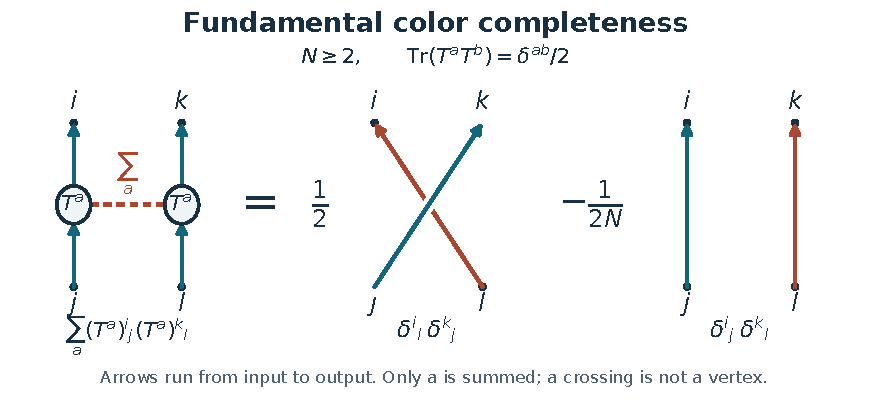
\includegraphics[width=\textwidth]{figures/second-pass-fierz.pdf}
\caption{The fundamental completeness relation with its four external indices and every coefficient. In this figure fundamental wires run vertically, from the explicitly labelled inputs to outputs. The dotted adjoint edge denotes summation over the normalized generators.}
\label{fig:second-pass-fierz}
\end{figure}

The first term on the right joins opposite fundamental legs; the second joins each pair without exchanging them. The factor $1/N$ and the factor $1/2$ are part of the theorem. A diagram that suppresses them is not the same invariant. This contraction is relevant to color indices in Yang--Mills calculations, but it evaluates a finite representation-theoretic factor. It supplies no continuum measure, renormalization estimate, or lower spectral bound. The earlier analytic obligations remain in force.

\section{Channels as positive tensors}

To discuss noisy circuits, learned measurements, and any proposed cross-aeon message, a linear amplitude map is insufficient. A density operator $\rho$ is positive semidefinite with trace one. A channel $\mathcal E:\End(H)\to\End(K)$ is completely positive and trace preserving. In the input-first convention its Choi tensor is
\[
 J_{\mathcal E}=\sum_{i,j}|i\rangle\langle j|\otimes
          \mathcal E(|i\rangle\langle j|).
\]
Here $|i\rangle\langle j|$ is a matrix unit; the outer input leg is conjugated when interpreted as a transformation rule under basis change. The convention is explicit so a transpose cannot be silently replaced by a dagger.

\begin{theorem}[Finite Choi--Kraus criterion]
\label{thm:choi-criterion}
Let $\mathcal E:\End(H)\to\End(K)$ be complex-linear. It is completely positive exactly when $J_{\mathcal E}\succeq0$. In that case there are matrices $K_\alpha:H\to K$ such that
\[
 \mathcal E(X)=\sum_\alpha K_\alpha X K_\alpha^\dagger.
\]
It is trace preserving exactly when
$\sum_\alpha K_\alpha^\dagger K_\alpha=I_H$, equivalently
$\Tr_KJ_{\mathcal E}=I_H$.
\end{theorem}
\begin{proof}
If $\mathcal E$ is completely positive, apply $\operatorname{id}_H\otimes\mathcal E$ to the positive operator $|\Omega\rangle\langle\Omega|$, where $\Omega=\sum_ie_i\otimes e_i$ in a basis-labelled copy of $H\otimes H$. Its image is $J_{\mathcal E}$.
Conversely diagonalize the positive matrix as $J=\sum_\alpha v_\alpha v_\alpha^\dagger$, incorporating square roots of eigenvalues into the vectors. Write
$v_\alpha=\sum_i e_i\otimes K_\alpha e_i$; this defines every matrix entry of $K_\alpha$ uniquely. The $(i,j)$ block of $J$ is then
$\sum_\alpha K_\alpha|i\rangle\langle j|K_\alpha^\dagger$.
Equality on matrix units proves the Kraus formula. Each map
$\operatorname{id}_m\otimes\mathcal E$ sends a positive $Y$ to
$\sum_\alpha(I_m\otimes K_\alpha)Y(I_m\otimes K_\alpha)^\dagger$, which is positive, proving complete positivity.
Finally cyclicity of the finite trace gives
$\Tr\mathcal E(X)=\Tr(X\sum_\alpha K_\alpha^\dagger K_\alpha)$.
The trace pairing is nondegenerate, so equality with $\Tr X$ for all matrix units is equivalent to the stated matrix identity. Taking the partial trace of the Choi formula gives the transpose of this sum; equality to $I$ is unchanged by transpose.
\end{proof}

The positive cone intersected with the affine partial-trace constraint gives a concrete feasible set for a learned channel. It differs from the affine variety $BA=0$: positivity is an inequality, not a polynomial equality over $\C$. With real and imaginary coordinates, the channel condition can be written as polynomial equalities together with nonnegative principal minors. This is a semialgebraic constraint. The geometry of complexes may constrain other blocks of a model, but it cannot replace the channel's positivity test.

An isometry or unitary circuit followed by a partial trace automatically produces a channel. A free matrix-valued neural output does not. One practical parameterization is to output a unitary dilation and trace an environment. Another is to parameterize Kraus operators and explicitly enforce their completeness relation. Renormalizing arbitrary operators without checking invertibility or the remaining constraints is not a proof of trace preservation.

\section{A precise grammar for the executable circuits}

We now separate three different questions. \emph{Generation} asks which finite graphs or circuit strings a grammar produces. \emph{Interpretation} maps each well-typed expression to a matrix or channel. \emph{Acceptance} asks what decision is made from a measurement or a classical computation on that interpretation. Their complexities can differ greatly.

For the finite laboratory let the wire type be $Q=\C^2$, with $1\le n\le6$. A gate record consists of a symbol from $\{H,X,Z,S,S^\dagger,T,T^\dagger,\mathrm{CX},\mathrm{SWAP}\}$ and a valid ordered list of distinct wire indices of the correct arity. A circuit is a sequence of such records; time runs from left to right and its matrix is the corresponding right-to-left product. Parameters such as $R_y(\theta)$ belong to a separate numerical experiment unless an angle alphabet or a computable encoding has been specified. Arbitrary real numbers are not a finite grammar alphabet.

A graph representation replaces each wire by a chain of directed edges and each gate by a typed vertex. Its input and output ports retain their order. In surface-constrained mode, allowed two-qubit gates must follow a supplied adjacency relation between data qubits on the cellulation. Relabelling vertices changes index names consistently, including the adjacency relation. A gate sequence is not a new dessin merely because it was rendered near a torus.

There are two useful kinds of production. A \emph{generative} production appends an allowed gate and changes the represented unitary. An \emph{equational} production replaces a subdiagram by an equal map and preserves the represented unitary. The laboratory's cancellation rule removes adjacent $U,U^\dagger$ on the same ordered wires. It also exposes commuting disjoint gates as an independently checked identity. No rule treats an approximate learned equality as exact.

\begin{theorem}[Typed rewrite soundness]
\label{thm:typed-rewrite-soundness}
Interpret a well-typed expression using composition, tensor product, and the specified generator maps. Suppose every equational rule $L\rightsquigarrow R$ has the same input and output type and $\llbracket L\rrbracket=\llbracket R\rrbracket$. Replacing any subexpression by such a rule preserves the full interpretation. For unitary circuit interpretations, every finite sequence of these replacements preserves every output measurement probability on every input density operator.
\end{theorem}
\begin{proof}
An expression with one hole is built from the hole by successively composing on either side with a fixed map or tensoring on either side with a fixed map. Equality is preserved by each operation, using bilinearity or simply substitution. Induction on this construction proves equality in every context. Induction on the number of rewrites proves equality after a finite derivation. Equal circuit matrices $U,V$ give equal operators $U\rho U^\dagger=V\rho V^\dagger$, and hence equal numbers $\Tr(MU\rho U^\dagger)$ for every measurement effect $0\preceq M\preceq I$.
\end{proof}

\begin{figure}[htbp]
\centering
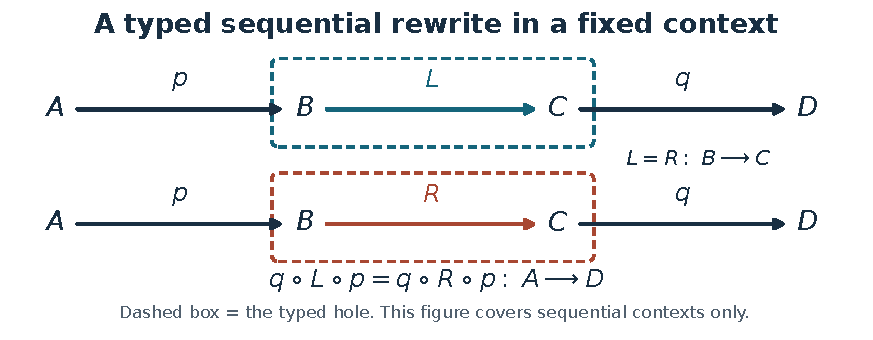
\includegraphics[width=\textwidth]{figures/second-pass-typed-context.pdf}
\caption{A typed sequential context. An equality of maps with the same domain and codomain can be substituted between fixed maps. The formal module checks this sequential syntax and finite derivations; tensor extensions are proved in the text.}
\label{fig:second-pass-context}
\end{figure}

The Lean file verifies the sequential linear-map part of this argument with a typed syntax and one-hole contexts. Tensor-context cases and density-operator consequences are proved in the text. This is an exact scope statement: checking the sequential theorem does not certify a parser, graphical embedding, tensor coherence theorem, or browser floating-point arithmetic.

\begin{proposition}[Termination and accumulated approximation error]
Repeated adjacent inverse cancellation terminates. If $U_j,V_j$ are unitary operators on the same Hilbert space and $\|U_j-V_j\|\le\epsilon_j$, then
\[
 \|U_m\cdots U_1-V_m\cdots V_1\|\le\sum_{j=1}^m\epsilon_j.
\]
For a unit input vector and a measurement effect of norm at most one, the resulting probability difference is at most $2\sum_j\epsilon_j$.
\end{proposition}
\begin{proof}
Every cancellation reduces the nonnegative integer number of gates by two. For the norm bound, insert products whose first $j$ factors have been replaced and telescope. Each difference is a left unitary product times $U_j-V_j$ times a right unitary product, so its norm is at most $\epsilon_j$. For output vectors $u,v$,
$\langle u,Mu\rangle-\langle v,Mv\rangle
=\langle u-v,Mu\rangle+\langle v,M(u-v)\rangle$.
Cauchy--Schwarz and $\|u\|=\|v\|=1$ give the stated bound.
\end{proof}

Termination is not completeness. A circuit with no adjacent inverse pair may still equal the identity; for example $(HZ)^8$ does. The chosen local simplifier is allowed to miss an equality. Its guarantee is that every equality it does apply is valid. A learned policy can rank applicable valid rewrites without changing this guarantee. If it is also allowed to propose new identities, a separate certificate or numerical-error bound must be checked before acceptance.

\section{How the grammar preserves a complex}

The varieties-of-complexes constraint can be carried through a learned representation without pretending that any graph mutation preserves it. Let
$C_2\xrightarrow{d_2}C_1\xrightarrow{d_1}C_0$ satisfy $d_1d_2=0$.

\begin{proposition}[Transport of a complex and its metric]
\label{thm:unitary-chain-transport}
Let $F_i:C_i\to C'_i$ be invertible linear maps and put
$d'_i=F_{i-1}d_iF_i^{-1}$. Then $d'_1d'_2=0$, and $F_1$ induces an isomorphism
$\ker d_1/\im d_2\cong\ker d'_1/\im d'_2$.
If the spaces carry Hilbert metrics and all $F_i$ are unitary, the middle Laplacians satisfy
\[
 d_1'^\dagger d'_1+d'_2d_2'^\dagger
 =F_1(d_1^\dagger d_1+d_2d_2^\dagger)F_1^{-1}.
\]
\end{proposition}
\begin{proof}
The middle inverse cancels in
$d'_1d'_2=F_0d_1F_1^{-1}F_1d_2F_2^{-1}=0$.
The same identities show $F_1(\ker d_1)=\ker d'_1$ and
$F_1(\im d_2)=\im d'_2$, giving a well-defined invertible quotient map. When $F_i^{-1}=F_i^\dagger$, taking adjoints of the transported differentials and cancelling the adjacent unitary factors gives the displayed conjugacy term by term.
\end{proof}

Invertibility alone gives homology invariance; it does not give this spectral equality for fixed metrics. This is the same algebra-versus-metric distinction encountered in lattice cryptography. A learned basis change should therefore specify whether it preserves the inner product, changes the metric along with the basis, or deliberately changes the spectrum.

\begin{proposition}[A controlled enlargement]
Adjoin the two-term complex $0\to W\xrightarrow{I}W\to0$ in any adjacent degrees, with zero couplings to the original complex. The direct-sum complex has the same homology as the original. With orthogonal direct-sum metrics its Laplacian gains an eigenvalue equal to one with multiplicity $\dim W$ in each of those two degrees.
\end{proposition}
\begin{proof}
The added identity has zero kernel and full image, so its two homology groups vanish. Kernels and images of a block-diagonal differential decompose into direct sums, yielding the homology assertion. On each new $W$ summand precisely one of $d^\dagger d$ and $dd^\dagger$ is $I$ and the other is zero. Thus its Laplacian block is $I$.
\end{proof}

This is an elementary grammar rule for increasing representation size with a proof of homological preservation. It is not automatically a geometric subdivision of a given surface; constructing the required cellular chain equivalence is an additional task. It also shows why preserving homology does not preserve a numerical gap unchanged: when $W\ne0$, a former gap greater than one in an affected degree becomes one after this enlargement.

\section{Expressivity: four different classifications}

The Chomsky hierarchy classifies languages of finite strings over a finite alphabet. A graph language enters that hierarchy only after a serialization and acceptance relation have been specified. The label ``context-free graph grammar'' does not assert that every natural string yield is a context-free language. Hyperedge replacement has its own gluing semantics and expressive distinctions \cite{TGhrg}.

\begin{proposition}[Bounded interfaces give bounded treewidth]
Consider a finite hyperedge replacement grammar. A production replaces one nonterminal hyperedge by a fixed finite graph with an ordered external interface; the only identifications are the prescribed attachment vertices, distinct external vertices remain distinct, and new internal vertices are fresh. Suppose every right-hand side and the initial graph has at most $b$ vertices. For every finite complete derivation, the primal graph of its terminal result has a tree decomposition of width at most $b-1$.
\end{proposition}
\begin{proof}
Use the derivation tree, with a root for the initial graph and one node for each replacement. At each node place in a bag the images in the final graph of all vertices in its right-hand side, including its external vertices; at the root use the initial vertices. Each bag has at most $b$ vertices. Every final vertex was either initial or introduced by a production and lies in its creating bag. Every pair of vertices made adjacent by a terminal hyperedge occurs together in the bag in which that hyperedge was introduced. Finally, a vertex can enter a descendant production only through the attachment interface of a hyperedge already containing it. Along the unique ancestry path from its creation to any later occurrence, it therefore remains in every intervening bag. Its bags form a connected subtree. These are exactly the covering, edge, and connectedness conditions for a tree decomposition.
\end{proof}

The bound applies to a fixed grammar with fixed finite production templates. It does not cover an arbitrary new gate layer supplied as an unbounded template, unbounded interfaces, or later identifications of distant vertices. In particular, a fixed bound cannot generate all increasingly large square grids: their treewidth is unbounded. This limits what a narrow-interface grammar can express on larger and higher-genus surface-code families.

\begin{proposition}[Context-free graph generation can have a non-context-free string yield]
A fixed-interface graph grammar with distinct attachment vertices can generate path graphs with edge labels
$a^n\#b^n\#c^n$, $n\ge1$. Their left-to-right string language, and its yield after erasing the two separators, are not context free.
\end{proposition}
\begin{proof}
Use a nonterminal with six distinct external vertices, the endpoints of three ordered paths. Its base production makes three one-edge paths labelled $a,b,c$. Its recursive production extends the first path by one $a$, the second by one $b$, and the third by one $c$, passing their new endpoints as the interface of one recursive occurrence. An initial production adds one separator-labelled edge from the end of the first path to the start of the second and another from the end of the second to the start of the third, producing one path without identifying any attachment vertices. Equivalently its three-component yield obeys
$(x,y,z)\mapsto(ax,by,cz)$ from $(a,b,c)$, followed by separator insertion. Induction gives the stated graph language and, after erasure, $\{a^nb^nc^n:n\ge1\}$.
If the latter language were context free, let $p$ be a pumping length and consider $a^pb^pc^p$. In any pumping decomposition with the central three-piece block of length at most $p$, that block meets at most two adjacent constant-letter blocks. Pumping the two designated pieces changes at least one count, leaves at least one of the three counts unchanged, and either destroys the letter order or makes the counts unequal. The pumped string is outside the language, contradicting the pumping property. Finally, erasing a terminal in the productions of a context-free grammar yields a context-free grammar for the erased language, allowing empty productions. Thus the separator-containing language cannot have been context free either.
\end{proof}

The example's final graphs are paths, so their treewidth is only one. Graph width, language yield complexity, and quantum simulation complexity are different quantities. The separator-erasing homomorphism is specified explicitly rather than hidden in an informal reading of the graph.

\begin{proposition}[Unrestricted effective graph rewriting can express Type-0 recognition]
Allow finite labelled graphs, local finite rewrite rules, unbounded graph growth, and acceptance when a distinguished accepting state is reached. This model can simulate every Turing machine. Its recognized input-string languages are exactly the recursively enumerable languages.
\end{proposition}
\begin{proof}
Represent a machine tape by a directed path of cells with symbol labels and a distinguished cell carrying the machine state. A transition changing symbol $a$ to $b$ and moving right is a local rewrite of the current head cell and its right neighbour: replace $a$ by $b$ and move the state marker to that neighbour. A second rule handles the end of the represented tape by creating a fresh blank cell. Left moves have analogous rules, with a fixed left-end marker for a one-sided tape. Since state and tape alphabets and the transition table are finite, there are finitely many rules. Induction on machine steps proves exact correspondence between configurations and reachable labelled paths. An accepting state is reached exactly when the machine accepts. Conversely, finite labelled graphs and finite rule matches have effective finite encodings. Breadth-first enumeration of finite derivations semi-decides whether an accepting graph is reachable. This gives the reverse inclusion.
\end{proof}

No general terminating algorithm decides all acceptance questions for that unrestricted model: such an algorithm would decide Turing-machine acceptance, contradicting diagonalization. Adding quantum amplitudes does not justify omitting computability assumptions on coefficients or providing a finite simulator with unbounded resources.

\begin{center}\small
\begin{tabular}{p{.25\linewidth}p{.32\linewidth}p{.34\linewidth}}
\toprule
Model & Precisely classified object & Consequence\\\midrule
Bounded browser laboratory & Finite circuits on at most six wires and a bounded gate count & A finite set; every serialization language is regular.\\
Fixed-width unbounded instruction strings & All well-typed instructions from a finite gate alphabet & Syntactic validity is regular; semantic equality is a different problem.\\
Finite-interface replacement grammar & Graphs glued through specified ports & A bounded-width graph class under the proposition's assumptions; string yields need not be context free.\\
Unrestricted effective rewriting & Existence of a finite accepting derivation & Type-0 recognition; general termination is undecidable.\\
Uniform polynomial quantum circuits & Bounded-error measurement decisions as input length grows & BQP, a computational complexity class, not an extra level of the Chomsky hierarchy.\\\bottomrule
\end{tabular}
\end{center}

For the last row, ``uniform'' means that a classical algorithm produces the size-$n$ circuit in polynomial time, using a fixed finite gate set with effectively computable entries. Bounded error means acceptance probability at least $2/3$ on yes instances and at most $1/3$ on no instances. Noncomputable real parameters would hide an oracle in the model. A fixed six-qubit browser demonstration is a finite numerical example, not evidence that an asymptotic BQP-hard problem has been solved efficiently.

\section{When the tensor grammar is also efficiently classical}

\begin{proposition}[Dynamic contraction along a derivation tree]
Suppose every tensor index has dimension at most $D$, each production has at most $q$ distinct local index variables including its external interface, and there are $m$ production instances. If child tensors are contracted and summarized at their prescribed interfaces, the final tensor can be computed with at most $O(mD^q)$ scalar operations, up to a fixed factor depending on the grammar. The bound assumes that the required final interface also fits within $q$.
\end{proposition}
\begin{proof}
Process the finite derivation tree from its leaves upward. At a production, the already computed child tensors and the finitely many local generator tensors have entries indexed by the at most $q$ local variables. Enumerate all their assignments, multiply the relevant entries, and add to the corresponding external-interface entry. There are at most $D^q$ assignments, and a fixed grammar bounds the number of factors per assignment. This computes exactly the contracted subdiagram by associativity and distributivity of finite sums. Summing the work over $m$ nodes proves the estimate.
\end{proof}

This explains an important tradeoff for quantum learning on diagrams. A bounded-interface family may be interpretable, trainable, and classically tractable for the same structural reason. It should be chosen for those benefits when appropriate; its tractability is not evidence of a quantum speedup. Conversely, allowing wide entangling interfaces can remove this contraction bound and make state-vector simulation exponential in the qubit count. The earlier GPU results distinguish dense amplitudes from stabilizer frames precisely for this reason.

The graph's usual treewidth is also not automatically the contraction width. A tensor of very high valence can have exponentially many entries even when the vertex graph is a star. The bound above controls the actual index interface. This supplies a concrete complexity budget for a quantum graph grammar rather than inferring computational efficiency from an attractive surface drawing.

\section{A learned rule selector with a checked semantic core}

A quantum or classical neural network may assign scores $s_\theta(r,G)$ to applicable rules $r$ on a current graph $G$. Mask ill-typed rules before forming a softmax. The learned policy chooses among the remaining rules; the certificate checker verifies the local algebraic condition. If all permitted moves are the equational moves of Theorem~\ref{thm:typed-rewrite-soundness}, every accepted derivation preserves the represented function regardless of the policy's weights. If moves instead generate candidate models, the learned score supplies a proposal distribution and carries no equality guarantee.

These two uses support different research tasks. For a toric code, a selector can simplify a stabilizer circuit using verified identities. For a variety of complexes, it can propose a basis transport with the invertibility or unitarity certificate required above. For a CMB inference problem, it can generate a family of source templates and rank their likelihoods, but the observational null calibration must include that selection process. For finite tokenization DAGs, the quantum ToricGT experiment below proposes paths and checks them against an exact shortest-path certificate. In every case the mathematical rule, the learned search heuristic, and the final certificate have distinct jobs.

An L-function or zeta function requires an additional arithmetic or spectral definition. A tensor determinant may be a characteristic polynomial, a finite partition function, or a local factor when the required operator has been specified. Merely labelling a closed diagram by $\zeta$ does not turn its contraction into the Riemann zeta function. Similarly, graph rewriting can preserve a determinant under a proved similarity or multiply it by a known factor under a block extension; a statement about its zeros then follows from that actual identity. The earlier convergence and nonvanishing conditions remain necessary for any passage to an infinite analytic object.

\section{Executable obligations}

The companion's grammar laboratory displays a circuit before and after inverse cancellation, the typed wire lists, the gate count, and the numerical maximum-entry difference between their full matrices. It shows the alternating projector's rank and closed-loop dimension, and verifies the two sides of the fundamental color contraction. Its language panel runs an exact integer-state recursive recognizer and contrasts bounded prefixes with the unbounded theorem proved in the next chapter. The executable checks have independent matrix or combinatorial references; a displayed small residual is floating-point evidence for those instances, while the propositions establish the general identities under their hypotheses.

This gives the requested birdtracks-level discipline: every wire has a space, every vertex has a tensor, every contraction has a summation, every scalar normalization is retained, and every rewrite has a precise soundness obligation. The interpretation remains equally valid when the graph is drawn in three dimensions or projected from four-dimensional coordinates; those visual choices do not alter its algebra.

\chapter{A trainable quantum interface for ToricGT}
\label{chap:quantum-toricgt}

\reviewstatus{This chapter supplies an original, bounded implementation and
elementary proofs for a quantum feature interface to a graph transformer.
It reports nine completed GPU training runs and independent numerical checks.
It does not identify this implementation with the complete upstream ToricGT
program, a biomolecular language model, or a quantum computer. The simulation
uses three qubits per graph token. Its exact path certificates are classical
mathematical certificates, with their own proofs and verification code.}

\section{Which architecture is being extended?}

A useful connection between algebra and learning begins with a precise
interface. A theorem about a ring, a circuit, or a chain complex does not
automatically become a theorem about a trained predictor. We therefore give
each part of the construction a separate role. Graph structure specifies
legal objects; a finite circuit supplies trainable features; a transformer
predicts a value function; and an independent checker determines what a
proposed solution actually establishes.

The implementation sources reviewed for this extension are pinned to
\texttt{amelie-iska/ToricGT} commit
\texttt{a5199bc989a6fb170e21220e5e87bf95bc2fc0b4} and
\texttt{amelie-iska/ToricGT-Program} commit
\texttt{f91ba1811b5a4f70d53c7120acf8ca2a0049f85b}.
The four source modules inspected in full implement graph tokenization,
tropical attention, finite Weyl matrices, and Soft-MoE routing. The program
overview requires empirical evaluation of proposed algebraic auxiliaries;
it does not make their utility follow from their names.
\cite{qtToricGTCode,qtToricGTProgram}

Our model retains vertex and edge tokens, endpoint incidence, a mixture of
ordinary and max-plus attention, and four experts with two slots each.
Its new component is a jointly trained circuit feature encoder. The older
repository example under \path{examples/quantum_tokengt} used a frozen
three-qubit feature construction and trained a classical attention head.
The present experiment trains both the input-to-angle map and twelve circuit
offsets. This is a concrete change in the optimization problem, not an
increase in the number of qubits. The larger surface-code circuits described
elsewhere in this monograph are separate experiments.

There are also deliberate changes to the upstream graph encoding. The
reviewed tokenizer contains learned identifier embeddings. Such a table is
not automatically invariant under arbitrary renaming of vertices. Here the
identifiers enter only through equality of endpoints, equivalently through
inner products of orthonormal identifier vectors. Intrinsic byte positions
remain ordinary input attributes. A permutation of storage order transports
these attributes; it does not change the underlying string. This distinction
will be used explicitly in the equivariance proof.

The ToricBLM source located during this review is the author's June 2026
proposal, which discusses graph tokens and affine steering regions. It is
useful as a design source. An independently pinned, trained ToricBLM
repository was not located in the reviewed material. Consequently this
chapter makes no claim to reproduce its proposed 100-million-parameter
biomolecular model, its biological validation program, or broad claims of
generalization.\cite{qtToricBLM}

The selected task is exact weighted tokenization on small directed acyclic
graphs. It gives the learner a meaningful combinatorial problem while
keeping the teacher and certificate transparent. This choice also makes a
limitation explicit: dynamic programming already solves the task efficiently.
The experiment tests whether a particular trainable representation works;
it does not establish a computational advantage over that algorithm.

\section{Tokenization graphs and exact solution certificates}

\subsection{The fixed-vocabulary problem}

Let a string have length $n$. Its byte boundaries are vertices
$0,1,\ldots,n$. An allowed token occupying the substring from boundary $i$
to boundary $j$ gives an edge $e:i\to j$, where $i<j$. An edge has integer
cost $c_e$. Every one-byte edge is available, so a path to $n$ exists from
every vertex. A complete tokenization is a directed path from $0$ to $n$.
In the experiment, candidate tokens have length at most three and the
alphabet has four symbols. Costs depend on a recorded, bounded control
parameter; the full graph and its costs are supplied to the model.

The colored-DAG formulation follows the tokenization viewpoint of
ConvexTok. Its vocabulary-selection problem and its decoding problem must
be distinguished. Choosing a globally shared vocabulary under a size budget
is a discrete optimization problem. Once the allowed vocabulary is fixed,
the remaining path problem on a DAG admits the elementary solution below.
\cite{qtConvexTok}

\begin{proposition}[Bellman recursion on a finite token DAG]
\label{qt:bellman}
Suppose all edges point from smaller to larger vertex indices and every
nonterminal vertex reaches $n$. Set $d(n)=0$ and, in decreasing order of $i$,
define
\[
 d(i)=\min_{e:i\to j}\{c_e+d(j)\}.
\]
Then $d(i)$ is the minimum cost of a path from $i$ to $n$. Choosing a
minimizing edge at every visited vertex produces an optimal path.
\end{proposition}
\begin{proof}
At $n$ the only path of length zero costs zero. Suppose the assertion holds
for vertices larger than $i$. Every path beginning at $i$ has a first edge
$i\to j$ and a remaining path beginning at $j$. By the induction hypothesis
its cost is at least $c_e+d(j)$, hence at least the displayed minimum.
Conversely choose an edge attaining the minimum and append an optimal path
from its target. The result attains $d(i)$. The graph is finite and every
edge strictly increases the index, so this procedure terminates. Backward
induction proves every assertion.
\end{proof}

The recursion works even with negative edge costs because there are no
directed cycles. Our sampled costs are positive, which makes their
interpretation as token costs convenient but is not needed for this proof.
With outgoing adjacency lists, the arithmetic work is linear in the number
of edges. This is the exact teacher used during dataset generation.

\begin{proposition}[A checkable primal--dual certificate]
\label{qt:path-certificate}
Let $p:V\to\R$ satisfy $p(n)=0$ and
\[
 p(i)-p(j)\leq c_e \qquad(e:i\to j).
\]
For every path $P$ from $0$ to $n$,
$p(0)\leq C(P):=\sum_{e\in P}c_e$.
If equality holds for one legal path, that path is optimal.
The Bellman distances in Proposition~\ref{qt:bellman} give such a potential
and equality on every path obtained by choosing minimizing edges.
\end{proposition}
\begin{proof}
Write the successive vertices of $P$ as $i_0=0,i_1,\ldots,i_m=n$.
Adding its $m$ inequalities gives
\[
 \sum_{r=0}^{m-1}c_{i_r i_{r+1}}
 \geq \sum_{r=0}^{m-1}(p(i_r)-p(i_{r+1}))
 =p(0)-p(n)=p(0).
\]
Thus $p(0)$ is a lower bound for every feasible solution. A path attaining
the bound is optimal. The Bellman minimum implies
$d(i)\leq c_e+d(j)$ for each outgoing edge, and a minimizing edge makes
this inequality an equality. Summing along the resulting path proves the
last assertion.
\end{proof}

The certificate checker verifies the token substrings, continuity of the
path, its endpoint, all potential inequalities, and equality of the final
cost and lower bound. It uses literal integers, rather than a numerical
tolerance. A learned value function $\widehat d$ supplies a candidate path
by minimizing $c_e+\widehat d(j)$ at each step. Rounded predictions supply
an initial integral potential. Backward replacement
\[
 p(i)\leftarrow\min\bigl(p(i),\min_{i\to j}(c_{ij}+p(j))\bigr)
\]
makes that potential feasible while preserving $p(n)=0$. Feasibility does
not force the proposed path to attain its lower bound. This is why the
experiment reports the frequency of an immediately certified learned
proposal separately from the frequency of a merely optimal learned path.

If the certificate does not close, an exact dynamic-programming repair is
available. The final output is then certified, but its certainty belongs
to the checker and repair algorithm. Calling this a perfect neural success
rate would conceal the distinction between prediction and verification.
The stored results retain the original proposal, its regret, its initial
certificate, whether repair was required, and the final certificate.

\subsection{A separate vocabulary-selection relaxation}

For completeness, consider several token DAGs with a shared finite set of
token colors $\mathcal C$. For each document let $f_e$ indicate whether an
edge is used, and let $y_c$ indicate whether a priced token color is included.
Byte edges need no color budget. With the incidence convention
$B e=e_{\mathrm{source}(e)}-e_{\mathrm{target}(e)}$, impose
\[
 Bf=e_s-e_t,\qquad f_e\leq y_{c(e)}\text{ on priced edges},\qquad
 \sum_c y_c\leq K.
\]
The integer program uses binary variables and minimizes the number, or
specified weighted cost, of used edges. Replacing binary variables by
intervals $[0,1]$ gives a linear relaxation. A rounded vocabulary must be
evaluated by decoding again; a fractional flow is not itself a vocabulary.
Our companion implements this small formulation on the three strings
\texttt{abca}, \texttt{bcab}, and \texttt{cabc} with budget two.

\begin{lemma}[Integral unit flows on an ordered DAG]
\label{qt:unit-flow}
Let every edge of a finite graph increase a fixed vertex order. If
$f\in\N^E$ and $Bf=e_s-e_t$, with distinct vertices $s$ first and $t$ last, then $f$ is the
incidence vector of one directed $s$--$t$ path.
\end{lemma}
\begin{proof}
At $s$, incoming flow is zero and outgoing flow is one. Integrality selects
exactly one outgoing edge of multiplicity one. Follow it. At an internal
vertex reached by a unit of flow, conservation supplies an outgoing edge
with positive integral multiplicity unless the vertex is $t$. Increasing
order prevents repetition and forces eventual arrival at $t$; otherwise a
last visited nonterminal vertex would violate conservation. Subtract this
path's flow from $f$. The remainder is nonnegative and has zero boundary.
A nonzero nonnegative flow with zero boundary on a DAG is impossible:
choose its first vertex incident to a positive outgoing edge. No positive
incoming edge can enter that vertex, contradicting conservation. Therefore
the remainder is zero.
\end{proof}

\begin{proposition}[An exact lower bound from a rational LP dual]
\label{qt:lp-dual}
For the real linear program
\[
 \min c^T x,\qquad Ax=b,\quad Hx\leq h,\quad 0\leq x\leq\mathbf1,
\]
suppose $y$ is unrestricted, $z\leq0$, $u\leq0$, and
$A^T y+H^Tz+u\leq c$ coordinatewise. Then every feasible $x$ satisfies
\[
 c^Tx\geq b^Ty+h^Tz+\mathbf1^Tu.
\]
If a feasible integer solution attains this lower bound, it solves both
the relaxation and the integer problem.
\end{proposition}
\begin{proof}
Multiply the coordinatewise dual inequality by $x\geq0$ and sum. This gives
$c^Tx\geq y^TAx+z^THx+u^Tx$. The equality constraint supplies $y^Tb$.
Because $z\leq0$ and $Hx\leq h$, one has $z^THx\geq z^Th$.
Because $u\leq0$ and $x\leq\mathbf1$, one has $u^Tx\geq u^T\mathbf1$.
Combining these bounds proves the claim. Integer feasible points form a
subset of the relaxation's feasible set, so equality proves optimality in
both problems.
\end{proof}

The numerical LP solver proposes multipliers. The checker converts them
to rational numbers and explicitly checks the displayed inequalities.
If rounding a proposed multiplier changes feasibility, the coordinate
correction
$u_j=\min(0,c_j-(A^Ty+H^Tz)_j)$ restores the required inequality.
The resulting exact lower bound for the recorded example is $6$.
Exhaustive enumeration of the allowed two-color vocabularies also gives
cost $6$. The equality certifies this particular finite example. It does
not assert that the relaxation is integral for arbitrary corpora.

\section{A finite Weyl encoder with trainable gates}

\subsection{The noncommutative algebra is explicit}

Let $q\geq2$, let $\omega=\exp(2\pi i/q)$, and index the standard basis of
$\C^q$ cyclically. Define
\[
 Ue_j=\omega^j e_j,\qquad Ve_j=e_{j-1}.
\]
The backward-shift convention fixes the sign in the commutation relation.
These are the finite matrices used as an algebraic ingredient in the
reviewed ToricGT module.\cite{qtWeylCode}

\begin{proposition}[Finite Weyl relations and matrix basis]
\label{qt:weyl}
The operators $U,V$ are unitary, $U^q=V^q=I$, and $VU=\omega UV$.
The $q^2$ matrices $U^rV^s$, $0\leq r,s<q$, are an orthogonal basis of
$M_q(\C)$ for the Hilbert--Schmidt inner product.
\end{proposition}
\begin{proof}
The diagonal entries of $U$ have modulus one and $V$ permutes an
orthonormal basis, so both are unitary. Their $q$th powers are the identity.
On $e_j$ the two products satisfy
$VUe_j=\omega^j e_{j-1}$ and $UVe_j=\omega^{j-1}e_{j-1}$, proving the
relation, including the cyclic case $j=0$ because $\omega^q=1$.

If $s\not\equiv0\pmod q$, $U^rV^s$ has zero diagonal and trace zero.
If $s=0$, its trace is $\sum_{j=0}^{q-1}\omega^{rj}$, equal to zero unless
$r=0$, when it equals $q$. Indeed, for $r\neq0$ the geometric sum multiplied
by $1-\omega^r$ is $1-\omega^{rq}=0$ and $1-\omega^r\neq0$.
Using the commutation relation, the product
$(U^rV^s)^*U^{r'}V^{s'}$ is a nonzero scalar times
$U^{r'-r}V^{s'-s}$. Its trace is therefore zero for distinct pairs and is
$q$ for identical pairs. There are $q^2$ nonzero orthogonal matrices in a
$q^2$-dimensional vector space, which proves the basis assertion.
\end{proof}

This finite algebra has a perfectly ordinary classical matrix
representation. The word ``noncommutative'' establishes neither quantum
hardware usage nor a computational speedup. In the implementation $q=8$;
one vector of dimension eight is represented by three qubits, not by eight
qubits or by three independent eight-level systems. A finite representation
at a rational phase parameter also does not by itself approximate every property of an
irrational noncommutative torus.

\subsection{Circuit and measurements}

For a token feature vector $x\in\R^8$, the input encoder computes six angles
\[
 a(x)=\pi\tanh(W_a x+b_a).
\]
There are two circuit layers. In layer $\ell\in\{0,1\}$, for each
$r\in\{0,1,2\}$ apply, in this order,
\[
 R_Y(a_r+\theta_{\ell r0}),\qquad
 R_Z(a_{r+3}+\theta_{\ell r1}),
\]
to qubit $r$, then apply controlled-NOT gates $0\to1$ and $1\to2$.
The initial state is $|000\rangle$ and qubit zero is the most significant
bit. There are twelve learned offsets $\theta_{\ell rb}$. The six input
angles are reused in both layers; this matters when differentiating the
input encoder.

For the resulting unit vector $\psi(x;\theta)$ define
\[
 f(x;\theta)=
 (\Re\langle U\rangle,\Im\langle U\rangle,
  \Re\langle V\rangle,\Im\langle V\rangle,
  \Re\langle UV\rangle,\Im\langle UV\rangle),
 \quad \langle T\rangle=\psi^*T\psi.
\]
These are real features. For a unitary $T$, its real and imaginary
expectations are expectations of the Hermitian operators
$(T+T^*)/2$ and $(T-T^*)/(2i)$. Thus the feature definition has a
measurement interpretation, although estimating several noncommuting
observables generally requires separate state preparations. The present
experiments calculate expectations in a classical statevector simulator;
they do not include shot noise or noisy physical gates.

\begin{lemma}[Normalization and feature bounds]
\label{qt:bounds}
The displayed circuit preserves norm. Each of its six real features lies
in $[-1,1]$. Moreover, for unit vectors $\psi,\varphi$ and an operator $T$
with $\|T\|\leq1$,
\[
 |\psi^*T\psi-\varphi^*T\varphi|\leq2\|\psi-\varphi\|.
\]
\end{lemma}
\begin{proof}
Both Pauli rotations are unitary and controlled-NOT is a permutation of an
orthonormal basis; their product preserves norm. Cauchy--Schwarz gives
$|\psi^*T\psi|\leq\|\psi\|\,\|T\psi\|\leq1$ for the three unitary
operators under consideration. Real and imaginary parts have no larger
absolute value. Finally write the expectation difference as
\[
 (\psi-\varphi)^*T\psi+\varphi^*T(\psi-\varphi)
\]
and apply the triangle inequality and Cauchy--Schwarz to the two summands.
\end{proof}

\subsection{What the parameter-shift formula actually differentiates}

The familiar two-evaluation rule applies to an expectation whose parameter
occurs in one gate with a two-eigenvalue generator. The general analytic
gradient framework is developed by Schuld and collaborators.
\cite{QSSchuld2019} The short proof here fixes the normalization and
the composition rule needed by this implementation.

\begin{proposition}[Single-occurrence Pauli parameter shift]
\label{qt:shift}
Let $P=P^*$, $P^2=I$, and
$R(t)=\exp(-itP/2)$. For fixed state $\eta$ and Hermitian $H$, put
$F(t)=\eta^*R(t)^*H R(t)\eta$. Then
\[
 F'(t)=\tfrac12\{F(t+\pi/2)-F(t-\pi/2)\}.
\]
The same identity holds for each real feature above when the varied
offset occurs in exactly one gate of that token's circuit.
\end{proposition}
\begin{proof}
The identity $P^2=I$ splits the exponential series into even and odd powers:
$R(t)=I\cos(t/2)-iP\sin(t/2)$. On expanding $R^*HR$, the coefficients of
$H$, $PHP$, and $i(PH-HP)$ are respectively
$\cos^2(t/2)$, $\sin^2(t/2)$, and $\sin(t/2)\cos(t/2)$.
Consequently $F(t)=A+B\cos t+C\sin t$ for real constants $A,B,C$.
Its derivative is $-B\sin t+C\cos t$, and the displayed shifted difference
has exactly this value. Gates preceding $R$ can be absorbed into $\eta$;
gates following it can be absorbed by conjugating $H$. Each real or
imaginary Weyl feature uses a Hermitian observable as explained above, so
the same argument applies to each feature.
\end{proof}

\begin{proposition}[Hybrid gradient with shared parameters]
\label{qt:chain-rule}
Let $f_{tj}(\theta)$ be feature $j$ of token $t$ and let a differentiable
classical computation give loss $L=\ell((f_{tj})_{t,j})$. If offset
$\theta_k$ occurs once in each token circuit, then
\[
 \frac{\partial L}{\partial\theta_k}
 =\sum_{t,j}\frac{\partial\ell}{\partial f_{tj}}
 \frac{f_{tj}(\theta_k+\pi/2)-f_{tj}(\theta_k-\pi/2)}2,
\]
where each difference changes only that occurrence in that token circuit
and the classical derivatives are evaluated at the original features.
If a parameter occurs in several gates, sum these contributions over its
occurrences before applying its outer chain rule.
\end{proposition}
\begin{proof}
Temporarily replace every gate occurrence by an independent variable.
The ordinary multivariable chain rule expresses the derivative of $L$ as
the sum of its feature adjoints multiplied by the feature derivatives.
Proposition~\ref{qt:shift} evaluates each such derivative. Identifying
occurrence variables with the shared parameter sums their derivatives,
again by the chain rule. This proves both statements.
\end{proof}

It would generally be incorrect to replace the derivative of the entire
nonlinear loss by half the difference of two shifted losses. For example,
if $f(t)=\cos t$ and $L(t)=f(t)^2$, those two shifted losses are equal,
whereas $L'(t)=-\sin(2t)$ is usually nonzero. The graph attention and
expert networks are nonlinear functions of the features. Our verification
therefore compares their feature adjoints composed with independent
parameter-shift Jacobians against automatic differentiation of the full
loss. At max-plus ties a classical derivative may fail to exist; the
implementation uses its framework's subgradient convention. The analytic
identity above is asserted at differentiability points, not as a unique
derivative at every tie.

The circuit offsets each have a single occurrence per token. An input
angle occurs once in each of the two layers, so its derivative has two
occurrence contributions. The input-to-angle map then contributes its
ordinary derivative $\pi\operatorname{sech}^2(W_ax+b_a)$. Automatic
differentiation performs this composition during training; the independent
shift check specifically audits the shared circuit offsets.

\section{A graph transformer whose symmetries can be stated precisely}

\subsection{Tokens and incidence}

For a vertex $i$, use endpoint pair $(i,i)$; for an edge $i\to j$, use
$(i,j)$. Each token has eight scalar attributes: vertex and edge indicators,
the two byte positions divided by twelve, token span divided by twelve,
cost divided by thirty-two, the bounded control divided by two, and the
edge's cost slope divided by two. Inapplicable entries are zero.
The endpoint-incidence matrix is
\[
 R_{tu}=\tfrac14\sum_{a,b=1}^2
   \mathbf1\{\operatorname{end}_a(t)=\operatorname{end}_b(u)\}.
\]
Equivalently replace the indicator by the inner product of orthonormal
endpoint vectors. This encoding uses equality structure, not a coordinate
choice in the identifier space. Vertex and edge tokenization has a primary
antecedent in TokenGT; its general expressivity results involve additional
architecture hypotheses and are not claimed for this small model.
\cite{qtTokenGT}

The initial hidden table is
\[
 X_t=W_x x_t+b_x+W_f f(x_t;\theta)+b_f\in\R^{24}.
\]
It has two graph blocks and two attention heads per block. Each block
normalizes token rows, forms learned queries, keys, and values, and centers
and normalizes each query and key before forming scores. For one head the
scores have the form
\[
 S_{tu}=\frac{q_t^T k_u}{\sqrt{12}}+\rho R_{tu},\qquad \rho>0.
\]
The two aggregation operations are
\[
 A^{\rm soft}_{t r}=\sum_u
 \frac{e^{S_{tu}}}{\sum_v e^{S_{tv}}}v_{ur},
 \qquad
 A^{\rm max}_{t r}=\max_u(S_{tu}+v_{ur}).
\]
A learned sigmoid gate mixes them. The head outputs are concatenated and
mapped back to width twenty-four with a residual connection. The graph
here is fully observed; no autoregressive next-byte probability is being
reported. A causal language model would require a separate reveal-order
mask and proof that endpoint attributes expose no future information.

\begin{lemma}[Associativity of finite max-plus contraction]
\label{qt:maxplus}
For finite compatible matrices with entries in
$\R\cup\{-\infty\}$, define
$(A\odot B)_{ik}=\max_j(A_{ij}+B_{jk})$, with the usual convention for
$-\infty$ and $\max\varnothing=-\infty$. Then $(A\odot B)\odot C=A\odot(B\odot C)$.
Splitting the contracted index set into blocks and taking the maximum of
the block maxima gives the same result.
\end{lemma}
\begin{proof}
Both parenthesizations at entry $(i,l)$ equal
$\max_{j,k}(A_{ij}+B_{jk}+C_{kl})$. Finite maxima can be taken in either
order. A maximum over a finite disjoint union is the maximum of the maxima
over its pieces, proving the second statement.
\end{proof}

This justifies an exact blockwise max-plus reduction when its scores and
values are already fixed. It does not make the whole graph network
piecewise affine in its raw input or in its parameters: normalized
queries and keys, their dot products, quantum expectations, softmax,
layer normalization, and GELU activations are nonlinear.

\subsection{Soft experts and a permutation proof}

For an $m\times d$ token table $X$ and eight learned slot keys, form logits
$L_{ts}$ by scaled cosine similarity. In the implementation each vector
$v$ is normalized as $v/\max(\|v\|_2,10^{-6})$, including the zero vector;
this convention is also used for the centered queries and keys. Row layer
normalization uses its population variance plus $10^{-5}$ under the square
root. These positive constants make every displayed row operation defined
at constant or zero rows. Define two differently normalized
arrays
\[
 D_{ts}=\frac{e^{L_{ts}}}{\sum_{u=1}^m e^{L_{us}}},\qquad
 C_{ts}=\frac{e^{L_{ts}}}{\sum_{r=1}^8 e^{L_{tr}}}.
\]
The slot inputs are $\widetilde X=D^TX$. Two slots are assigned to each
of four learned feed-forward experts, giving output slots
$\widetilde Y$. The token output is $C\widetilde Y$, multiplied by a
learned residual coefficient. Dispatch normalizes over tokens; combination
normalizes over slots. Confusing those axes changes the model.
\cite{qtSoftMoE}

\begin{proposition}[Equivariance of the implemented mathematical architecture]
\label{qt:equivariance}
Let $P$ be a permutation matrix on the valid tokens of a nonempty graph.
Transport token attributes and incidence by $X\mapsto PX$ and
$R\mapsto PRP^T$. Every displayed graph block and the rowwise readout
commute with this action. Thus the predicted node values are permuted
along with the corresponding node tokens. A coordinated renaming of
endpoint identifiers also leaves the incidence data unchanged.
\end{proposition}
\begin{proof}
Rowwise affine maps, rowwise normalizations, coordinatewise activations,
and the identical token circuit commute with left multiplication by $P$.
Queries, keys, and values therefore transform to $PQ,PK,PV$, so their
score matrix transforms to $PSP^T$. Row softmax transforms by the same
two-sided permutation, and its product with the permuted values is the
permutation of the original output. For max-plus attention, relabeling
the finite maximizing index merely reorders the same candidates, giving
the same conclusion. Residual addition and concatenation preserve it.

For the expert layer, $L$ transforms to $PL$. Consequently dispatch and
combination transform to $PD$ and $PC$. The slot inputs are unchanged:
$(PD)^T(PX)=D^TX$. Each expert acts on those unchanged slots, so the
output slots are unchanged. Multiplication by $PC$ permutes the final
token outputs. Induction over the blocks and the final rowwise readout
proves the assertion. Finally, a bijective renaming preserves every
endpoint equality appearing in $R$, which proves the last statement.
\end{proof}

The claim concerns attributed graphs. Changing a byte position while
keeping a token in place changes an attribute and can change the answer.
Likewise, erasing edge direction or swapping the semantic source and
target is not the token-storage permutation in the proposition. Masks
must be transported too when padding or causal restrictions are present.
In exact mathematics, padded keys are absent from sums and maxima. The
implementation checks the relevant finite-precision masking behavior
numerically, including insertion of padding and token permutations.

\section{Toric path relations, graph rewrites, and steering regions}

\subsection{A small commutative algebra with an exact graph meaning}

Let $G$ be a finite directed graph and give its edge variables the incidence
degrees $d_e=e_{\mathrm{target}(e)}-e_{\mathrm{source}(e)}\in\Z^V$,
the columns of a matrix $D$. Thus $D=-B$ for the flow matrix above, which does not
change the kernel. Consider the algebra map
\[
 \Phi:k[z_e:e\in E]\longrightarrow
 k[t_v^{\pm1}:v\in V],\qquad
 z_e\longmapsto t_{\mathrm{target}(e)}/t_{\mathrm{source}(e)}.
\]
For a nonnegative exponent vector $u$, its image has exponent vector
$Du$ with this incidence convention. Multiplication forgets the order
in which edges were listed; it retains their net boundary.

\begin{proposition}[The binomial kernel of the boundary code]
\label{qt:binomial-kernel}
The kernel of $\Phi$ is the ideal generated by all
$z^u-z^v$ with $u,v\in\N^E$ and $Du=Dv$.
In particular, two directed paths with the same initial and final vertices
have the same image under $\Phi$.
\end{proposition}
\begin{proof}
Every displayed binomial maps to zero. Conversely write a polynomial in
the kernel as a finite sum $\sum_u c_u z^u$ and group its terms according
to the integer vector $Du$. Distinct Laurent monomials are linearly
independent over $k$. Thus within each group the coefficients sum to zero.
Choose one exponent $u_0$ in a nonempty group. That group's contribution
equals $\sum_{u\ne u_0}c_u(z^u-z^{u_0})$, a sum of the stated binomials.
Adding the finitely many groups proves the kernel assertion. Along a path,
the incidence columns telescope to $e_t-e_s$, proving the final claim.
\end{proof}

For three arrows $a:0\to1$, $b:1\to2$, and $c:0\to2$, the two complete
paths give the relation $z_a z_b-z_c$. In this example the whole kernel is
$(z_a z_b-z_c)$. One may eliminate $z_c$, leaving the polynomial ring in
$z_a,z_b$; their incidence vectors are linearly independent, so their
images satisfy no further polynomial relation. The unit-flow polytope is
\[
 (f_a,f_b,f_c)=(\lambda,\lambda,1-\lambda),\qquad0\leq\lambda\leq1.
\]
The two integer endpoints are the two tokenizations. For edge costs
$c_a,c_b,c_c$, the preferred endpoint changes on the wall
$c_a+c_b=c_c$. The same comparison determines which side of the path
binomial is selected by the corresponding weight. This is an explicit
connection among a graph problem, a polytope, a binomial ideal, and a
piecewise-linear optimal value function.

The kernel relation alone does not certify an arbitrary sequence of
rewrite operations. The vector $u-v$ may have negative entries, and
applying it to a current state may leave the nonnegative orthant.
Even nonnegative boundary-preserving changes on a cyclic graph can add
a disconnected circulation. The DAG and unit-flow hypotheses in
Lemma~\ref{qt:unit-flow} are what turn a nonnegative solution with the
correct boundary into one legal path.

\begin{proposition}[A constrained rewrite preserves legal tokenization]
\label{qt:rewrite}
On the ordered DAG of Lemma~\ref{qt:unit-flow}, let $x$ be a legal path
flow and let $\delta\in\Z^E$ satisfy $B\delta=0$.
If $x+\delta\geq0$ coordinatewise, then $x+\delta$ is another legal
path flow with the same endpoints. Its cost change is exactly $c^T\delta$.
\end{proposition}
\begin{proof}
Linearity gives $B(x+\delta)=Bx+B\delta=e_s-e_t$.
The assumed nonnegative integral vector therefore satisfies
Lemma~\ref{qt:unit-flow} and is a path. The cost identity follows by
distributivity: $c^T(x+\delta)-c^Tx=c^T\delta$.
\end{proof}

A graph grammar can use such a local replacement when its interface and
nonnegativity tests are explicit. If declared path relations are made
columns of a map $\partial_2:C_2\to C_1$, their zero boundary gives
$\partial_1\partial_2=0$. A replacement by $\partial_2 w$ preserves the
homology class of a cycle. This is a genuine chain-complex connection to
the earlier chapters. It is weaker than proving that every algebraically
equivalent trajectory is semantically interchangeable. Dependencies,
labels, resource limits, and external facts need their own preservation
conditions. The commutative algebra records the chosen invariant; it
cannot reconstruct information intentionally discarded by abelianization.

\subsection{Affine margins and nonlinear circuit coordinates}

Suppose a finite decision system uses affine scores
$\ell_j(z)=a_j^Tz+b_j$ on a feature space. A fixed strict sign pattern of
these scores determines an open polyhedral region. It may be empty, and
there may be many disconnected regions after pulling it back through a
nonlinear encoder. The affine-space statement is the useful part of the
steering proposal; identifying a region with a scientifically correct
reasoning mechanism would require additional evidence.

\begin{proposition}[Preserving a finite affine sign pattern]
\label{qt:margin}
Let $s_j\in\{-1,1\}$ and suppose
$s_j\ell_j(z)\geq\gamma>0$ for every $j$. If
$|a_j^T\Delta z|<\gamma$ for every $j$, then
$s_j\ell_j(z+\Delta z)>0$ for every $j$.
In particular it suffices that
$\|\Delta z\|_2<\gamma/\max_j\|a_j\|_2$ when the denominator is positive.
If every $a_j=0$, every perturbation preserves the signs.
\end{proposition}
\begin{proof}
For each $j$,
$s_j\ell_j(z+\Delta z)=s_j\ell_j(z)+s_j a_j^T\Delta z
\geq\gamma-|a_j^T\Delta z|>0$.
Cauchy--Schwarz gives the sufficient norm bound. If all coefficients
vanish, all scores are constant.
\end{proof}

The proof applies, for example, to a finite list of path-cost comparisons
when the edge costs depend affinely on $z$. To use it in circuit parameters
one also needs a bound on the feature change. Here is a directly proved
bound for the twelve independent offsets, with the token input held fixed.

\begin{lemma}[A conservative circuit-offset perturbation bound]
\label{qt:circuit-lipschitz}
For the token circuit above and two offset vectors $\theta,\theta'$,
\[
 \|\psi(\theta')-\psi(\theta)\|
 \leq\tfrac12\|\theta'-\theta\|_1,
 \qquad
 \|f(\theta')-f(\theta)\|_2
 \leq\sqrt6\,\|\theta'-\theta\|_1.
\]
\end{lemma}
\begin{proof}
For a Pauli rotation the derivative has operator norm $1/2$.
Integrating along the real angle interval gives
$\|R(t')-R(t)\|\leq|t'-t|/2$.
Subtract two products of unitary gates by replacing one factor at a time.
The operator norm of each difference term is at most the norm difference
of that one factor, because all other factors are unitary. The sum over
the twelve independently varied gates proves the state bound.
Lemma~\ref{qt:bounds} then bounds the absolute change of each of the six
features by $\|\theta'-\theta\|_1$. Summing their squared bounds proves
the second inequality.
\end{proof}

Combining these propositions gives a sufficient margin condition for an
\emph{affine readout directly on the six features}. It does not give the
same constant for the full transformer. The latter's nonlinear layers
and learned weights contribute further Lipschitz factors; max-plus ties
also require the appropriate nonsmooth interpretation. Moreover a
polyhedron in expectation-feature space need not have a polyhedral
preimage in angle space. Even the one-qubit feature $\cos\theta$ has
periodic, nonlinear level sets. This qualification prevents a useful
local sign guarantee from becoming an unsupported global geometry claim.

\section{Three source corrections with complete small counterarguments}

The reviewed ToricGT V text contains several elementary interfaces that
are useful when their hypotheses are retained. The following localized
qualifications concern its saturation example, a sign in its predictive
transfer definition, and a proposed monotonicity interpretation of
coverage homology. The original pinned sources are preserved. The review
ledger records the exact commit, path, and line ranges; the corrections
here are new mathematical explanations, not silent edits to that source.
\cite{qtToricGTAlgebra}

\subsection{Saturation is relative to the generated lattice}

\begin{proposition}[The parity semigroup is normal in its own group]
\label{qt:parity-normal}
Let
$Q=\N(2,0)+\N(0,2)+\N(1,1)\subseteq\Z^2$. Then
\[
 \operatorname{gp}(Q)=\{(a,b)\in\Z^2:a+b\text{ is even}\},
 \qquad
 Q=\operatorname{gp}(Q)\cap\R_{\geq0}^2.
\]
In particular $Q$ is saturated in $\operatorname{gp}(Q)$, and $(1,0)$ is
not a saturation hole in that group.
\end{proposition}
\begin{proof}
Each generator has even coordinate sum, so every integer combination
does too. Conversely if $a+b$ is even, then $a-b$ is even and
$(a,b)=((a-b)/2)(2,0)+b(1,1)$ is an integer combination of generators.
This proves the group description.

For nonnegative $(a,b)$ with even sum, the coordinates have the same
parity. If both are even, use $(a/2)(2,0)+(b/2)(0,2)$. If both are odd,
use $((a-1)/2)(2,0)+((b-1)/2)(0,2)+(1,1)$. All coefficients are
nonnegative integers, proving the intersection formula. If
$m(a,b)\in Q$ with $m>0$ and $(a,b)\in\operatorname{gp}(Q)$, then
$a,b\geq0$, so the formula implies $(a,b)\in Q$.
Finally $(1,0)$ has odd coordinate sum and is outside the generated group.
\end{proof}

The fact that $2(1,0)\in Q$ does not contradict normality: its antecedent
omits membership in $\operatorname{gp}(Q)$. If one instead studies the
larger ambient lattice $\Z^2$, that is a different lattice specification.
This is the same distinction that matters when proving normality of the
semigroup degenerations in the standard-monomial chapters.

\subsection{Inclusions do not make Betti numbers monotone}

\begin{proposition}[A point, a circle, and a filled triangle]
\label{qt:betti-counterexample}
There exist inclusions of finite simplicial complexes
$K_0\subset K_1\subset K_2$ for which the first Betti numbers over
$\Q$ are $0,1,0$, respectively. Thus inclusion alone implies neither
nondecreasing nor nonincreasing first Betti numbers.
\end{proposition}
\begin{proof}
Take $K_0$ to be vertex $0$, $K_1$ the boundary of the triangle on
vertices $0,1,2$, and $K_2$ the filled triangle. In $K_1$, orient the
edges $0\to1$, $1\to2$, $2\to0$. The boundary matrix is
\[
 \partial_1=
 \begin{pmatrix}-1&0&1\\1&-1&0\\0&1&-1\end{pmatrix}.
\]
Its first two columns are independent and its three columns sum to zero,
so its rank is two and its kernel is spanned by $(1,1,1)^T$.
There are no two-simplices in $K_1$, giving $\dim H_1(K_1;\Q)=1$.
In $K_2$, orient the added triangle so that
$\partial_2(1)=(1,1,1)^T$. This map has rank one and its image equals
$\ker\partial_1$; hence $H_1(K_2;\Q)=0$.
The point has no one-chains, so $H_1(K_0;\Q)=0$ as well.
\end{proof}

A growing coverage complex can create a class and later kill it. A
statement that a support construction grows under evidence addition may
be correct while a monotone ``hole penalty'' conclusion is not justified.
One must specify induced homology maps, persistence intervals, and what
the complexes represent. Even a genuine persistent class is a property
of that representation, not a theorem that a scientific assertion is
false or that all relevant evidence has been gathered.

\subsection{Use one sign for predictive gain}

For normalized predictive distributions with positive probabilities on
the observed symbols, define the unaugmented codelengths
\[
 C_0=-\sum_t\log_2q_0(b_t\mid b_{<t}),\qquad
 C_1=-\sum_t\log_2q_1(b_t\mid b_{<t}).
\]
Their gain is
\[
 C_0-C_1=\sum_t\log_2\frac{q_1(b_t\mid b_{<t})}
                                  {q_0(b_t\mid b_{<t})}.
\]
If a deployed auxiliary costs $B$ additional bits, the total codelength
gain is $C_0-C_1-B$. Positive gain means improvement with this convention.
For a single observed symbol with $q_0=1/4$ and $q_1=1/2$, the
unaugmented gain is one bit. Reversing the ratio gives minus one bit.
Artifact-adjusted gain and ordinary predictive bits per byte should be
named separately, rather than changing the metric's definition mid-proof.
These identities say nothing about the task accuracy of a neural model
unless the probabilities and evaluation protocol have been supplied.

The companion's \path{algebra_checks.py} verifies the displayed boundary
ranks and zero composition exactly over $\Q$, checks the parity
decomposition on $545$ bounded pairs, and records the rational probability
example. The general semigroup claim follows from its proof above, not
from finite enumeration. The finite checks provide reproducible
illustrations and catch transcription mistakes.

\section{Completed learning experiment and numerical evidence}

\subsection{Protocol and comparators}

The fixed dataset contains $512$ training graphs and $128$ graphs in each
of the validation, test, and length-shift sets. All underlying strings
are distinct across the four sets. Training, validation, and ordinary
test strings have lengths four through eight; the length-shift set has
lengths nine through twelve. Token availability and integer cost parameters
are sampled from the recorded generator. Each byte fallback costs sixteen
integer units. In the following tables one unit of reported cost equals
that byte-fallback cost, so integer teacher costs are divided by sixteen.
The network itself predicts distances divided by thirty-two.

All three model variants use the same graph encoder layout, width
twenty-four, two attention blocks, four experts per block, and scalar node
readout. The trainable quantum and classical variants each contain
$25{,}515$ trainable parameters. The classical feature comparator uses
the same six encoded angles and twelve phase parameters, with bounded
features
\[
 g_j(a;p)=\tfrac12\bigl(\sin(a_j+p_j)
             +\cos(a_{j-1}+p_{j+6})\bigr),\qquad j\pmod6.
\]
The other input and graph layers are identical. This is a matched
parameter-count comparator, not a claim that it exhausts possible
classical architectures. In the frozen-circuit ablation, both the
$54$-parameter angle encoder and twelve circuit offsets are frozen, while
the remaining $25{,}449$ parameters are trained.

Each variant is trained at seeds $17,29,43$ for eighty epochs, batch size
thirty-two, AdamW learning rate $0.0015$, weight decay $10^{-4}$, and a
cosine learning-rate schedule ending at one tenth of its initial value.
The loss is mean squared error over valid node predictions, with padded
and edge-token targets excluded. The same initialization seed and
minibatch ordering are used for the corresponding variants. For each run,
the checkpoint with lowest validation node loss is selected before its
test and length-shift metrics are computed. The representative browser
checkpoint is the quantum run with lowest validation loss, not a
checkpoint chosen for its test score. A preceding two-epoch smoke run
checked execution and export; its results were not candidate checkpoints
for the reported experiment.

The runs used PyTorch $2.8.0$ with CUDA $12.8$ on an NVIDIA GeForce RTX
4090. They were classical GPU statevector simulations with analytic
expectations and automatic differentiation, not quantum-hardware
experiments and not cuStateVec training. The existing environment was
used without changing its packages. Process allocation was capped at
one tenth of GPU memory. The largest measured PyTorch allocation during
the nine runs was $183{,}426{,}048$ bytes, about $175$ MiB; this allocator
measurement does not include every CUDA-context allocation or the memory
of other applications. The full set of runs completed in approximately
$109$ seconds.\cite{qtExperiment}

\subsection{Results, including the negative evidence}

Table~\ref{qt:benchmark} reports means and sample standard deviations over
the three seeds. ``Optimal'' refers to the original learned proposal.
The initial certificate is stricter: the proposal must attain the lower
bound produced from its rounded, repaired potential. A proposal may be
optimal even when that particular potential does not certify it.
All final paths pass exact certification after the separately reported
dynamic-programming repair where required.

\begin{table}[htbp]
\centering\small
\begin{tabular}{llrrr}
\toprule
Set & Variant & Node RMSE & Optimal (\%) & Initial cert. (\%)\\
\midrule
Test & Trainable quantum & $0.265\pm0.003$ & $83.85\pm2.39$ & $24.74\pm0.45$\\
Test & Classical & $0.266\pm0.009$ & $84.38\pm0.78$ & $30.47\pm5.63$\\
Test & Frozen quantum & $0.284\pm0.011$ & $83.07\pm1.97$ & $25.78\pm5.12$\\
\midrule
Longer & Trainable quantum & $0.684\pm0.150$ & $54.69\pm3.41$ & $6.51\pm3.85$\\
Longer & Classical & $0.790\pm0.117$ & $50.00\pm4.75$ & $5.47\pm3.41$\\
Longer & Frozen quantum & $0.676\pm0.069$ & $52.86\pm0.90$ & $9.90\pm2.26$\\
\bottomrule
\end{tabular}
\caption{Measured learning outcomes on the fixed token-DAG dataset.
Uncertainty entries are sample standard deviations over three seeds,
not confidence intervals or statistical significance claims.}
\label{qt:benchmark}
\end{table}

The mean proposal cost regret on the ordinary test set is $0.0386$ for
the trainable quantum model, $0.0356$ for the classical comparator, and
$0.0399$ for frozen quantum features. On longer strings these means are
$0.2246$, $0.2625$, and $0.2324$, respectively. The mixed ordering is
substantive evidence: the classical comparator has slightly better
ordinary-test path accuracy and regret, while the trainable quantum model
has somewhat better mean path accuracy and regret under this length shift.
Frozen quantum features have a slightly lower mean length-shift node
RMSE than the trainable circuit. Three seeds on one synthetic task do not
support a general superiority conclusion for any of the variants.

The twelve quantum offsets change by Euclidean norms $0.146$, $0.151$,
and $0.158$ at the selected checkpoints, while the corresponding changes
in the frozen ablation are exactly zero. Initial gradients for the
circuit offsets and angle encoder are recorded. This establishes that
the new circuit feature map participates in training. It does not show
that every parameter is identifiable, that all gradients are equally
useful, or that optimization found a global minimum.

A batch of thirty-two graph forwards takes approximately $2.56$ ms for
the trainable quantum variant and $1.81$ ms for the classical comparator
on the measured GPU, after warm-up and synchronization. These are small
model-forward timings, excluding exact path repair and data preparation.
The exact dynamic program is an algorithmic baseline with zero regret;
the model comparison does not establish an end-to-end speed advantage
over it. No inference about a physical quantum device follows from these
classical timings.

\subsection{Independent checks and browser execution}

The circuit is implemented three ways: indexed PyTorch tensor operations,
independent dense NumPy Kronecker matrices, and a dependency-free JavaScript
statevector reference. The GPU verification uses double precision and
reports a maximum PyTorch--NumPy state difference of $3.73\cdot10^{-16}$,
feature difference of $4.45\cdot10^{-16}$, and automatic-differentiation
versus parameter-shift Jacobian difference of $3.34\cdot10^{-16}$ on
the recorded cases. The full nonlinear-loss chain-rule check differs by
$1.12\cdot10^{-16}$. These are observed numerical agreement bounds on
finite tests, not formal floating-point error theorems.

The same verification includes forty-eight independent exhaustive path
enumerations, exact rational LP-dual checks, token permutation and
padding checks, and the two normalization axes of the expert router.
Finite differences provide an additional numerical gradient check, but
the analytic parameter-shift identity is the mathematical reference.
All source and dataset hashes associated with the training runs are
retained. Checkpoints use ordinary NumPy array archives, and per-example
predictions and certificates are stored in JSON. The complete results
of all nine runs are retained, including the runs that do not favor
the quantum variant.

The browser runs the whole selected graph model. Its
\texttt{runGraph} function accepts the graph, exported weights and optional
circuit offsets. It recomputes input
angles, circuit expectations, both attention blocks, expert routing,
node predictions, and the candidate path. The optional offset tensor
has shape $2\times3\times2$. It changes the circuit offsets for every
token and propagates the resulting features through the full model.
The interface then checks the candidate and, if necessary, displays the
separate exact repair. Recorded predictions are not substituted for the
live computation.

JavaScript uses double arithmetic and an approximation to the error
function in GELU. Against saved GPU predictions on two ordinary-test and
two length-shift graphs, the largest discrepancy in normalized node
prediction is $6.81\cdot10^{-7}$. The four learned paths and final exact
certificates agree. Increasing one circuit offset by $0.4$ radians changes
the full model's predictions by as much as $0.555$ in the checked example;
the interactive control therefore changes the actual model computation.
This comparison is recorded with the hashes of the JavaScript modules
and exported weights.\cite{qtExperiment}

\section{Connections that follow, and research questions that remain}

The finite Weyl algebra is the strongest direct connection to quantum
algorithm theory in this experiment. Clock and shift matrices encode
finite translation and character operations. Similar algebra is central
to finite Fourier analysis. Here, however, their expectations are learned
features of a very small circuit. No hidden subgroup is identified, no
elliptic-curve discrete logarithm is extracted, and no improvement to
Shor's complexity follows. The earlier cryptographic chapters identify
the additional problem-specific structures required for those claims.

The binomial path kernel connects more directly to the standard-monomial
and semigroup chapters. It is an actual quotient map with a proved kernel,
and its simplest path comparison is an actual initial-term wall. The
parity example shows why the lattice used for normalization must be
specified. A hidden feature called a ``toric coordinate'' is not by
itself a point on a chosen toric variety; one must supply the monomial
map, relations, and any positivity or saturation hypotheses. Our finite
path construction supplies those data in an elementary setting.

Graph rewrites connect to complexes through the condition
$\partial_1\partial_2=0$ and to learning through proposal and acceptance.
A trainable model may suggest a boundary-preserving replacement; exact
checks enforce the interface and nonnegativity constraints. This is a
practical division of labor for a graph grammar. Extending it to arbitrary
typed hypergraphs requires the appropriate matching and gluing conditions,
which are developed separately in the graph-rewrite chapter. It is not
justified by a count-vector identity alone.

There is also a useful possible quantum extension whose theorem can be
stated independently of its implementation. It makes precise what it
would mean for a variational state to remain within a declared feasible
space. It is not the circuit trained in the preceding experiment.

\begin{proposition}[A constraint-preserving variational interface]
\label{qt:feasible-hilbert}
Let $\Omega$ be a finite set, $F\subseteq\Omega$ nonempty, and
$\Pi_F$ the orthogonal projector onto the span of basis vectors
$|x\rangle$ with $x\in F$. Let $\psi_0$ be a unit vector in this subspace.
If every gate $G_j$ is unitary and commutes with $\Pi_F$, the resulting
state $\psi=G_m\cdots G_1\psi_0$ remains in that subspace. Measurement in
the indicated basis returns an element of $F$ with probability one.
For a real cost function $c$ on $F$, put
$H_c=\sum_{x\in F}c(x)|x\rangle\langle x|$ on this subspace and
$c_* =\min_{x\in F}c(x)$. Then
$\langle H_c\rangle\geq c_*$. If every nonoptimal cost is at least
$c_*+\Delta$ for some $\Delta>0$, the probability of a nonoptimal outcome
is at most $(\langle H_c\rangle-c_*)/\Delta$.
\end{proposition}
\begin{proof}
Commutation gives
$\Pi_F G_j\eta=G_j\Pi_F\eta=G_j\eta$ whenever $\Pi_F\eta=\eta$.
Induction proves subspace preservation, and unitarity preserves norm.
Writing $\psi=\sum_{x\in F}\alpha_x|x\rangle$ gives
$\sum_x|\alpha_x|^2=1$ and
$\langle H_c\rangle=\sum_x c(x)|\alpha_x|^2$.
This is a convex combination of costs and is at least $c_*$.
Subtracting $c_*$ and retaining only nonoptimal terms yields
\[
 \langle H_c\rangle-c_*
 \geq\Delta\sum_{x:c(x)>c_*}|\alpha_x|^2,
\]
which is the claimed probability bound.
\end{proof}

To make this a useful algorithm one must efficiently encode $F$, prepare
$\psi_0$, construct expressive gates commuting with its projector, and
estimate the cost. Those are substantial additional tasks. In particular,
the three-qubit feature circuit in this chapter has no basis state for
every tokenization path of an arbitrary graph. Its unitarity certifies
normalization, while the separate graph checker certifies tokenization.
Confusing these two invariants would erase the main proof boundary.

Finally, the finite graph and tensor operations do not by themselves
establish a continuum gauge theory, an elliptic index theorem, a positive
Yang--Mills mass gap, or a cosmological model. They can provide finite
data structures and exactly checked algebraic interfaces for such
research. A field-theoretic or cosmological conclusion additionally
requires the physical interpretation, limiting procedure, analytic
hypotheses, and observational tests appropriate to that problem. The
cosmology and gauge-theory chapters retain those requirements. The
achievement established here is narrower and concrete: a source-grounded
trainable quantum graph feature model, explicit mathematical guarantees
for its finite interfaces, measured comparator results, and a live
reproducible implementation.



\part{Quantum fields and a precise research synthesis}
\chapter{Gauge fields, curvature, and the meaning of a complex}
\label{chap:gauge}

\section{The precise connection to the preceding algebra}

The theory of orders concerns modules carrying a multiplication action.  The
theory of complexes concerns maps whose consecutive compositions vanish.  Gauge
theory adds a third ingredient: the maps are differential operators depending on
a connection, and the obstruction to their composing to zero is curvature.
This observation supplies a concrete bridge between the subjects, but it also
identifies the hypothesis that any proposed bridge must preserve.  An arbitrary
covariant exterior derivative is not a differential in a cochain complex.
Its square is a curvature action.  A flat connection removes that obstruction;
an anti-self-dual connection removes the appropriate projected obstruction.
Neither operation turns a classical deformation problem into a construction of
the quantum vacuum.

The following derivations fix conventions sufficiently explicitly to permit
comparison with both algebraic complexes and formal proofs.  The foundational
gauge theory dates to Yang and Mills; the geometric analysis of the
anti-self-dual deformation complex is due to Atiyah, Hitchin, and Singer
\cite{YM1954,AHS1978}.  The proofs below are elementary derivations of the
identities used here.  The analytic index formula and reconstruction theorems
are identified separately as external results.

Let $M$ be a smooth, oriented Riemannian manifold without boundary and let
$G$ be a compact Lie group.  Let $P\to M$ be a principal $G$-bundle and write
$\operatorname{ad}P=P\times_{\operatorname{Ad}}\mathfrak g$.  Choose an
$\operatorname{Ad}$-invariant positive definite inner product on
$\mathfrak g$.  If $G$ is realized as a compact matrix group in $U(m)$, a
positive multiple of $-\operatorname{Re}\operatorname{Tr}(XY)$ is an example
on its skew-Hermitian Lie algebra.  The numerical multiple matters when
comparing coupling constants, instanton charges, and short-distance
coefficients.  It does not change the differential identities.

The affine space of smooth connections has tangent space
$\Omega^1(M;\operatorname{ad}P)$.  In a local trivialization a connection is
a Lie-algebra-valued one-form $A$, with
\begin{equation}
 F_A=dA+\tfrac12[A\wedge A],\qquad
 d_A\alpha=d\alpha+[A\wedge\alpha].
 \label{eq:curvature-conventions}
\end{equation}
For homogeneous forms the bracket includes exterior multiplication and the
Lie bracket.  In coordinates this means
\[
 (F_A)_{\mu\nu}=\partial_\mu A_\nu-\partial_\nu A_\mu+[A_\mu,A_\nu],
 \qquad D_\mu X=\partial_\mu X+[A_\mu,X].
\]
The bracket is graded antisymmetric:
$[\alpha\wedge\beta]=-(-1)^{pq}[\beta\wedge\alpha]$ for degrees $p,q$.
In particular it is symmetric for two one-forms.  Keeping this sign is
essential in the second variation.

\begin{proposition}[Curvature is the failure of the complex identity]
For every adjoint-valued form $\alpha$,
\begin{equation}
 d_A^2\alpha=[F_A\wedge\alpha],\qquad d_AF_A=0.
 \label{eq:curvature-square}
\end{equation}
Consequently, if $F_A=0$, the sequence
$\Omega^0(\operatorname{ad}P)\xrightarrow{d_A}
\Omega^1(\operatorname{ad}P)\xrightarrow{d_A}\cdots$ is a complex.
\end{proposition}

\begin{proof}
For a degree-zero section $s$, direct expansion gives
\[
 (D_\mu D_\nu-D_\nu D_\mu)s
 =[\partial_\mu A_\nu-\partial_\nu A_\mu,s]
   +[A_\mu,[A_\nu,s]]-[A_\nu,[A_\mu,s]]
 =[F_{\mu\nu},s],
\]
where the last equality is the Jacobi identity.  Antisymmetrizing the same
calculation in the additional form indices gives the first identity for every
degree; differentiation of the scalar form coefficients contributes the
ordinary identity $d^2=0$.  Equivalently, the graded Leibniz rule and graded
Jacobi identity give
$d_A^2=[dA+\frac12[A\wedge A],\cdot]$ directly.
For the second identity, the cyclic sum of
$D_\lambda F_{\mu\nu}$ has cancelling second derivatives and cancelling
first-derivative brackets.  The remaining terms are
$[A_\lambda,[A_\mu,A_\nu]]$ and their cyclic permutations, whose sum is
zero by Jacobi.  This is precisely $d_AF_A=0$.  If $F_A=0$, the first
identity says that every consecutive composition is zero.
\end{proof}

One must not reverse the last implication without a hypothesis on the
representation.  A central curvature can act trivially in the adjoint
representation.  For instance an abelian connection may have nonzero
curvature although its induced adjoint differential is the ordinary exterior
derivative.  For a centerless Lie algebra the statement that
$[F_A,\phi]=0$ for every local adjoint section $\phi$ does force $F_A=0$.
This qualification is a small example of the semantic checks required when a
formal statement is used as a bridge between different mathematical settings.

\section{Gauge covariance and the variational equations}

Use the convention
$A^u=u^{-1}Au+u^{-1}du$ for a gauge transformation $u$.
Then $d_{A^u}(u^{-1}\alpha u)=u^{-1}(d_A\alpha)u$ and
$F_{A^u}=u^{-1}F_Au$.  These formulas can be checked in a local matrix
representation by differentiating $u^{-1}u=1$.  Since the chosen inner
product is invariant, the Yang--Mills functional
\begin{equation}
 S(A)=\frac{1}{2g^2}\int_M |F_A|^2\,d\operatorname{vol}
 \label{eq:yang-mills-action}
\end{equation}
is gauge invariant.  Here $g>0$ is fixed.  On a noncompact manifold all
variations used below have compact support, or sufficient decay to justify
integration by parts.  On a manifold with boundary a boundary condition must
be supplied; omitting that condition changes the Euler--Lagrange problem.

\begin{proposition}[First and second variations]
For $a,b\in\Omega^1(M;\operatorname{ad}P)$,
\begin{align}
 F_{A+ta}&=F_A+t\,d_Aa+\tfrac12t^2[a\wedge a],\label{eq:curvature-variation}\\
 DS_A(a)&=g^{-2}\langle d_A^*F_A,a\rangle_{L^2},\label{eq:ym-first}\\
 D^2S_A(a,b)&=g^{-2}\left(
 \langle d_Aa,d_Ab\rangle_{L^2}
 +\langle F_A,[a\wedge b]\rangle_{L^2}\right).
 \label{eq:ym-second}
\end{align}
Thus a smooth connection is stationary for all permitted variations if and
only if $d_A^*F_A=0$.
\end{proposition}

\begin{proof}
Substitute $A+ta$ into \eqref{eq:curvature-conventions}.  The linear terms
are $da+[A\wedge a]=d_Aa$ because the bracket of one-forms is symmetric.
The quadratic term is $\frac12t^2[a\wedge a]$.  Differentiating
$\frac12g^{-2}\langle F,F\rangle$ once gives
$g^{-2}\langle F_A,d_Aa\rangle$, which equals
$g^{-2}\langle d_A^*F_A,a\rangle$ by the definition of the formal
adjoint.  Mixed differentiation of $F_{A+sa+tb}$ gives
$\partial_s\partial_tF=[a\wedge b]$.  Applying the product rule to the
norm square proves the Hessian formula.  If the first variation vanishes
for every compactly supported $a$, the fundamental lemma of the calculus of
variations gives the stated equation; its converse follows from the formula.
\end{proof}

The equation $d_AF_A=0$ is an identity, while $d_A^*F_A=0$ is a field
equation.  Their different logical roles are important.  Imposing the first
does not restrict the set of connections, whereas imposing the second
selects the classical Yang--Mills critical points.  In a Lean development the
Bianchi identity should be proved from the definition of curvature, not
added as an unexplained assumption that could conceal an inconsistent
definition.

The infinitesimal gauge direction is $d_A\phi$, because
$\frac{d}{dt}|_{t=0} A^{\exp(t\phi)}=d_A\phi$.  At a critical point,
the Hessian annihilates these directions in its associated bilinear form.
One way to see this without a coordinate calculation is to differentiate
the gauge invariance identity twice along a gauge orbit and a transverse
variation.  The term involving acceleration of the orbit is paired with
$DS_A$, which is zero at a critical point.  Thus the degeneracy is forced by
symmetry, and the unmodified Hessian cannot be elliptic on all one-forms.

For a nonzero covector $\xi$, omit the harmless factor $i$ in the symbol
convention.  The principal symbol of $d_A$ is exterior multiplication by
$\xi$; that of its adjoint is contraction by $\xi^\sharp$, up to the
consistent sign for a first-order adjoint.  The principal symbol of the
nonnegative second-order operator $d_A^*d_A$ on one-forms is
\[
 a\longmapsto |\xi|^2a-\xi\,\iota_{\xi^\sharp}a.
\]
It vanishes on multiples of $\xi$.  Adding the gauge-fixing term
$d_Ad_A^*$ changes this to $|\xi|^2a$.  Curvature contributes only
lower-order terms to the Hessian.  Accordingly the gauge-fixed Hessian is
elliptic, although its lower-order part need not be positive at an arbitrary
critical point.  Ellipticity concerns invertibility of the principal symbol;
positivity is a separate property of the complete operator.

\section{Four dimensions and self-duality}

Suppose now that $\dim M=4$.  On two-forms the Hodge star satisfies
$*^2=1$, and hence
\[
 \Lambda^2=\Lambda^2_+\oplus\Lambda^2_-,\qquad
 F_A^\pm=\tfrac12(F_A\pm *F_A).
\]
The two summands are orthogonal.  Define
$Q(A)=\int_M\langle F_A\wedge F_A\rangle$, where the invariant
pairing is extended to forms.  Then
\begin{equation}
 \|F_A\|_2^2=\|F_A^+\|_2^2+\|F_A^-\|_2^2,
 \qquad Q(A)=\|F_A^+\|_2^2-\|F_A^-\|_2^2.
 \label{eq:energy-topology}
\end{equation}
For a closed manifold, $Q(A)$ is constant as the connection varies on a
fixed bundle.  Its normalization as an integral characteristic number depends
on the representation and the invariant form.

\begin{proposition}[Energy bound and classical minimizers]
With the conventions above,
$S(A)\geq |Q(A)|/(2g^2)$.  Equality holds exactly when one of
$F_A^+$ or $F_A^-$ vanishes.  Every such connection satisfies the
Yang--Mills equation.
\end{proposition}

\begin{proof}
For nonnegative $x,y$, $x+y\geq|x-y|$, with equality if and only if
$xy=0$.  Apply this to the squared norms in
\eqref{eq:energy-topology}.  A smooth form with zero $L^2$ norm is zero,
so equality is the self-dual or anti-self-dual condition.  If
$*F_A=\pm F_A$, then $d_A*F_A=\pm d_AF_A=0$ by Bianchi.  The
formula for the formal adjoint, $d_A^*=\pm *d_A*$ in the relevant
degree, therefore gives $d_A^*F_A=0$.
\end{proof}

For completeness, the connection independence of $Q$ follows directly from
the first variation.  Differentiation gives
$2\int_M\langle d_Aa\wedge F_A\rangle$.
Invariance of the pairing and Bianchi identify the integrand with
$d\langle a\wedge F_A\rangle$.  Stokes' theorem makes the integral
zero on a closed manifold.  The statement requires an additional boundary
analysis on noncompact spaces; finite action alone should not be silently
substituted for all the boundary hypotheses needed in a particular theorem.

This is a useful first encounter with a topological quantity controlling an
analytic variational problem.  It is nevertheless a statement about
classical connections.  It gives neither an interacting quantum Hilbert
space nor a positive lowest nonzero quantum energy.  In particular a
positive action of a nontrivial instanton is not the mass of a lowest
particle.  The action of a Euclidean field configuration and the spectrum
of a reconstructed Hamiltonian are different objects.

\section{The anti-self-dual deformation complex}

At an anti-self-dual connection, $F_A^+=0$.  Linearization of this equation
gives $d_A^+a=0$, where $d_A^+=\pi_+d_A$.  Quotienting by
infinitesimal gauge transformations leads to
\begin{equation}
 0\longrightarrow\Omega^0(\operatorname{ad}P)
 \xrightarrow{d_A}\Omega^1(\operatorname{ad}P)
 \xrightarrow{d_A^+}\Omega^2_+(\operatorname{ad}P)
 \longrightarrow0.
 \label{eq:asd-complex}
\end{equation}
The following proof gives both parts of the assertion that this is an
elliptic complex.  Having the correct ranks is not by itself sufficient:
one needs the composition identity and exactness of the symbol at every
nonzero cotangent vector.

\begin{theorem}[Exactness of the anti-self-dual symbol sequence]
If $F_A^+=0$, then $d_A^+d_A=0$.  For every nonzero covector $\xi$,
the symbol sequence of \eqref{eq:asd-complex} is exact.
\end{theorem}

\begin{proof}
For an adjoint section $\phi$, the curvature identity gives
$d_A^+d_A\phi=\pi_+[F_A,\phi]=[F_A^+,\phi]=0$.
For symbol exactness the Lie algebra factor is passive, so it suffices to
work with ordinary real forms.  Rescale and choose an oriented orthonormal
coframe $e^1,e^2,e^3,e^4$ with $\xi=|\xi|e^1$.  The first symbol sends
$c$ to $c\xi$ and is injective.  If
$a=\sum_j a_je^j$, the second sends it to
\[
 \frac{|\xi|}{2}\sum_{j=2}^4a_j
 \left(e^1\wedge e^j+*(e^1\wedge e^j)\right).
\]
The three parenthesized forms are mutually orthogonal and nonzero, and
they span the three-dimensional self-dual space.  The map is therefore
surjective and its kernel consists precisely of multiples of $e^1$.
This kernel is the image of the first symbol.  Tensoring the exact
finite-dimensional sequence with $\mathfrak g$ preserves exactness.
\end{proof}

The proof displays a direct algebraic connection to varieties of complexes:
each nonzero cotangent vector determines a pair of linear maps satisfying a
zero-product equation and a particular exact rank condition.  The geometric
content is the existence of a smooth family of these maps, with specified
homogeneity in $\xi$, over the punctured cotangent bundle.  A single
algebraic complex cannot replace that family.  Its global symbol class is
the input to index theory.

Let $H_A^0,H_A^1,H_A^2$ denote the cohomology of
\eqref{eq:asd-complex}.  On a closed manifold elliptic theory makes these
spaces finite dimensional and gives harmonic representatives after choosing
Sobolev completions.  Their meanings are distinct: $H_A^0$ contains
infinitesimal stabilizers, $H_A^1$ infinitesimal deformations modulo gauge,
and $H_A^2$ obstructions.  The operator
\[
 L_A=d_A^*\oplus d_A^+:
 \Omega^1(\operatorname{ad}P)\longrightarrow
 \Omega^0(\operatorname{ad}P)\oplus\Omega^2_+(\operatorname{ad}P)
\]
has index $\dim H_A^1-\dim H_A^0-\dim H_A^2$.
At an irreducible, unobstructed connection this is the local dimension of
the moduli space.  Without those conditions the same integer is a virtual
dimension, not an assertion that the quotient is a manifold.

\begin{theorem}[Atiyah--Hitchin--Singer index formula, external]
For an $SU(2)$ bundle on a closed, connected, oriented Riemannian four-manifold,
write $k=\langle c_2(P\times_{SU(2)}\mathbb C^2),[M]\rangle$ with
the convention in which anti-self-dual instantons have positive $k$.
Then
\begin{equation}
 \operatorname{ind}L_A=8k-3(1-b_1(M)+b_2^+(M)).
 \label{eq:asd-index}
\end{equation}
\end{theorem}

This external theorem is an application of the analytic index theorem to
the symbol just computed \cite{AHS1978}.  The proof of the symbol
calculation above is not a proof of the index theorem.  On $S^4$ the
formula becomes $8k-3$ for the unframed irreducible problem.  Framing at
a point removes the three-dimensional constant gauge quotient in the usual
regular situation and gives $8k$.  Comparing these numbers without
recording framing conventions creates a spurious disagreement.

\section{A finite-dimensional algebraic model: monads and ADHM}

There is a stronger bridge than a resemblance between equations.  The
Atiyah--Drinfeld--Hitchin--Manin construction relates appropriate
finite-dimensional algebraic data to framed instantons
\cite{ADHM1978}.  We use only its elementary complex identity here, and
state the correspondence as an external theorem rather than re-proving its
analytic and algebro-geometric foundations.

Let $V,W$ be finite-dimensional complex vector spaces.  Choose
$B_1,B_2\in\operatorname{End}(V)$,
$I\in\operatorname{Hom}(W,V)$, and
$J\in\operatorname{Hom}(V,W)$.  Set
\[
 \mu_{\mathbb C}=[B_1,B_2]+IJ.
\]
For $z=(z_1,z_2)\in\mathbb C^2$, define
\[
 \alpha_z(v)=((B_1-z_1)v,(B_2-z_2)v,Jv),
 \quad
 \beta_z(v_1,v_2,w)=-(B_2-z_2)v_1+(B_1-z_1)v_2+Iw.
\]
Their types are $V\to V\oplus V\oplus W\to V$.  Direct
multiplication gives
\begin{equation}
 \beta_z\alpha_z=[B_1,B_2]+IJ=\mu_{\mathbb C}.
 \label{eq:adhm-composition}
\end{equation}
Thus the complex moment-map equation is exactly a zero-composition
condition, valid simultaneously for all $z$.

If $\alpha_z$ is injective and $\beta_z$ surjective for every relevant
$z$, the middle cohomology has dimension $\dim W$.  Indeed
$\dim\ker\beta_z=2\dim V+\dim W-\dim V$, and quotienting
by the $\dim V$-dimensional image of $\alpha_z$ leaves $\dim W$.
These constant-rank conditions give a vector bundle locally.  They are
essential: the equation $\mu_{\mathbb C}=0$ alone permits rank drops
and singular objects.

For unitary instantons the real moment-map equation also enters:
\[
 [B_1,B_1^*]+[B_2,B_2^*]+II^*-J^*J=0.
\]
Together with the appropriate stability and regularity conditions, the
data modulo the unitary action on $V$ yield the ADHM correspondence.
The complex equation explains why varieties of complexes are relevant;
the real equation, positivity, and rank conditions explain why arbitrary
points of a variety of complexes are insufficient.  In particular this
construction describes classical instantons.  Its finite-dimensional
algebra does not prove a quantum mass gap or an algorithm for elliptic-curve
discrete logarithms.

The monad identity is also a good candidate for machine checking: matrix
multiplication, commutators, scalar identities, and dimensions have clear
finite specifications.  Formalizing the full ADHM correspondence would
require extensive differential geometry and analysis beyond that elementary
identity.  Reporting the identity as ``the ADHM theorem verified'' would
discard almost all of the theorem's content.

\section{Why an index cannot establish a quantitative gap}

An index records a difference of dimensions.  A spectral gap is an
inequality with a positive numerical constant.  The distinction can be
proved by an example that is already a complex of finite-dimensional
vector spaces.

\begin{proposition}[Exactness does not control the smallest singular value]
For every $\varepsilon>0$, the complex
$0\to\mathbb R\xrightarrow{\varepsilon}\mathbb R\to0$ is exact,
but the smallest eigenvalue of either associated nonzero Laplacian is
$\varepsilon^2$.  There is no positive lower bound valid for all
$\varepsilon>0$.
\end{proposition}

\begin{proof}
Multiplication by a nonzero real number is a bijection, so both cohomology
groups vanish.  Relative to the standard inner products, the adjoint is
also multiplication by $\varepsilon$, and $d^*d=dd^*=\varepsilon^2$.
For any proposed lower bound $c>0$, choosing
$0<\varepsilon<\sqrt c$ contradicts the bound.
\end{proof}

The same phenomenon appears geometrically.  On a flat torus of side length
$L$, the scalar Laplacian has eigenvalues
$(2\pi/L)^2|n|^2$ for $n\in\mathbb Z^d$.  The first positive one is
$4\pi^2/L^2$, which tends to zero as $L\to\infty$.  Each fixed torus
has a compact elliptic problem and a discrete spectrum, yet no
volume-independent positive gap follows.  The quantum Yang--Mills problem
contains a much more difficult version of precisely this issue: a bound
must survive both the ultraviolet limit and unbounded physical volume.

This gives a disciplined place for orders and homological algebra.  They
can organize integral models, modules, deformation complexes, characteristic
classes, and exact relations among observables.  To conclude a mass gap
one still needs coercive estimates or spectral information with constants
that remain positive in the required limits.  The absence of such an
estimate is a mathematical missing implication, not a matter of choosing
more persuasive terminology.

\chapter{From finite gauge lattices to a quantum spectral gap}
\label{chap:quantum-gap}

\section{Three different uses of the word lattice}

A lattice over an order is a module with a finiteness and torsion-freeness
condition over the ground ring.  A Euclidean lattice is a discrete subgroup
of a real inner-product space, with a metric that makes shortest-vector and
decoding questions meaningful.  A lattice in a lattice gauge theory is a
discrete approximation to spacetime, equipped with vertices, links, and
plaquettes.  The first two notions can be related by embeddings of number
fields and choices of positive forms.  The third need not carry any order
module structure at all.  Identifying all three because they share a word
would erase their defining mathematical data.

There are productive interactions nevertheless.  A gauge theory on a finite
cell complex has incidence maps and chain groups.  A choice of coefficient
ring can make those chain groups modules over an order.  Discrete Hodge
operators add positive inner products.  Fourier analysis on finite abelian
groups, central in quantum algorithms, also diagonalizes many free lattice
operators.  Each such connection is a construction that can be specified
and proved.  None entails that the computational hardness of a Euclidean
lattice problem controls the mass spectrum of an interacting gauge theory.

\section{A finite Wilson model exists by elementary integration}

Let a finite oriented cell complex have a set $E$ of positively oriented
edges and a set $\mathcal P$ of oriented plaquettes.  Assign $U_e\in G$ to
each $e\in E$, and use $U_{\bar e}=U_e^{-1}$ for the reverse orientation.
The ordered product around a plaquette is $U_p$.  For a fixed unitary
representation $G\subset U(m)$ and $\beta\geq0$, define
\begin{equation}
 E_W(U)=\sum_{p\in\mathcal P}
 \left(1-\frac1m\operatorname{Re}\operatorname{Tr}U_p\right),\quad
 Z_\beta=\int_{G^E}e^{-\beta E_W(U)}\prod_{e\in E}dh(U_e),
 \label{eq:wilson-finite}
\end{equation}
where $h$ is normalized Haar measure.  Wilson's lattice construction
preserves gauge invariance before taking any limit \cite{Wilson1974}.
The following modest result explains exactly how much existence is obtained
from compactness alone.

\begin{proposition}[Finite-volume normalization and gauge invariance]
The quantity $Z_\beta$ satisfies
$e^{-2\beta|\mathcal P|}\leq Z_\beta\leq1$, and
$d\mu_\beta=Z_\beta^{-1}e^{-\beta E_W}\prod_e dh(U_e)$ is a
probability measure.  It is invariant under the vertex gauge action
$U_{xy}\mapsto t_xU_{xy}t_y^{-1}$.
\end{proposition}

\begin{proof}
Every eigenvalue of a unitary matrix has modulus one, so
$-m\leq\operatorname{Re}\operatorname{Tr}U_p\leq m$.
Thus $0\leq E_W\leq2|\mathcal P|$ and
$e^{-2\beta|\mathcal P|}\leq e^{-\beta E_W}\leq1$.
Integration against a probability measure gives the bounds.  In particular
the normalization is finite and strictly positive.
Under a vertex transformation the successive $t_y^{-1}t_y$ factors in a
plaquette cancel, leaving conjugation by the transformation at its initial
vertex.  Trace is invariant under conjugation, so the action is unchanged.
Haar measure on a compact group is invariant under both left and right
translations.  Applying this separately to each edge preserves the product
measure and proves the last assertion.
\end{proof}

The proof works for every finite complex and every compact matrix group.
It contains no control as the number of plaquettes tends to infinity or as
the lattice spacing tends to zero.  The lower bound on $Z_\beta$ itself
degenerates exponentially with $|\mathcal P|$.  Dividing by $Z_\beta$
produces a probability measure, but does not remove the need for uniform
bounds on the observables whose limits one wants to take.

An observable such as a product of finitely many matrix entries is bounded
at fixed lattice spacing.  A renormalized curvature observable typically
contains negative powers of the spacing and cutoff-dependent mixing with
other observables.  Its bound can diverge as the spacing tends to zero.
Consequently, compactness of $G$ is compatible with difficult and highly
singular continuum limits.  The relevant estimates must concern the
renormalized observables and their correlations, not merely the unscaled
link variables.

\section{Reflection positivity is additional structure}

Let $\vartheta$ reflect Euclidean time and let $\mathcal A_+$ denote a
space of observables supported at positive times.  Write
$\Theta F=\overline{F\circ\vartheta}$, with any required adjoint on
field labels.  Reflection positivity asserts
\begin{equation}
 \mathbb E[(\Theta F)F]\geq0\qquad(F\in\mathcal A_+).
 \label{eq:reflection-positive}
\end{equation}
It is not a consequence of the ordinary positivity of a probability measure.
For example, take a symmetric random variable $Z$ with
$0<\mathbb E[Z^2]<\infty$ and set $X_+=Z$, $X_-=-Z$.
The joint law is a positive probability measure and is invariant under
exchanging the two time labels.  Nevertheless, for $F=X_+$,
$\mathbb E[(\Theta F)F]=\mathbb E[X_-X_+]=-\mathbb E[Z^2]<0$.
Both positivity and reflection symmetry can hold while reflection positivity
fails.

The Wilson action has the special structure needed for appropriate lattice
reflection-positivity and transfer-matrix theorems
\cite{OSSeiler1978,Luscher1977}.  A useful finite-dimensional ingredient
can be proved directly.

\begin{proposition}[Positive-type Wilson link weight]
Let $\rho:G\to U(m)$ be a unitary representation, $\chi(g)=\operatorname{Tr}\rho(g)$,
and $c\geq0$.  The function $w(g)=\exp(c\operatorname{Re}\chi(g))$
is of positive type: for all $g_1,\ldots,g_n\in G$ and
$z_1,\ldots,z_n\in\mathbb C$,
\[
 \sum_{i,j}\overline{z_i}z_jw(g_i^{-1}g_j)\geq0.
\]
\end{proposition}

\begin{proof}
The character $\chi$ is of positive type because
\[
 \sum_{i,j}\overline{z_i}z_j\chi(g_i^{-1}g_j)
 =\operatorname{Tr}\left(
  \Bigl(\sum_i z_i\rho(g_i)\Bigr)^*
  \Bigl(\sum_j z_j\rho(g_j)\Bigr)\right)\geq0.
\]
The conjugate character is the character of the conjugate unitary
representation.  Products of characters are characters of tensor products.
Expanding
\[
 w(g)=\sum_{a,b\geq0}\frac{(c/2)^{a+b}}{a!b!}
                  \chi(g)^a\overline{\chi(g)}^{b}
\]
therefore expresses $w$ as a limit of nonnegative linear combinations of
positive-type functions.  Since $|\chi(g)|\leq m$, the double series
converges uniformly.  For any fixed finite set of points and coefficients,
the associated nonnegative quadratic forms converge to the displayed
quadratic form, which remains nonnegative.
\end{proof}

This lemma proves a kernel positivity statement.  The full lattice theorem
also needs a factorization compatible with the reflection plane, the
orientation of links, and the integration of gauge variables.  Those
additional steps are not omitted by calling the lemma a proof of the full
Osterwalder--Schrader reconstruction theorem.  The separation of claims is
particularly useful in a formal development: a locally verified kernel
identity can be reused without overstating its global consequence.

\section{The Hilbert-space quotient behind reconstruction}

Reflection positivity supplies the semidefinite sesquilinear form
$(F,G)_{\mathrm{OS}}=\mathbb E[(\Theta F)G]$.
Assume that the correlation functional is defined on a complex vector
space $\mathcal V_+$ of finite positive-time field words, that this form
is Hermitian, and that it is nonnegative on the diagonal.  The following
quotient step is purely algebraic.

\begin{proposition}[Null vectors and positive quotient]
For a positive semidefinite Hermitian form $B$ on a complex vector space,
the set $N=\{v:B(v,v)=0\}$ is a linear subspace and
$B(v,w)=0$ for every $v\in N$ and $w$.  The induced form on
$\mathcal V_+/N$ is positive definite.
\end{proposition}

\begin{proof}
If $B(w,w)>0$, positivity of
$B(v+\lambda w,v+\lambda w)$ for every $\lambda\in\mathbb C$
and minimization of this real quadratic polynomial gives
$|B(v,w)|^2\leq B(v,v)B(w,w)$.  If $B(w,w)=0$, apply the same
argument to $w+\varepsilon u$ with a positive-norm $u$ and pass to the
limit, or examine the linear term of the polynomial directly.  Thus
Cauchy--Schwarz holds in all cases.  If $v\in N$ it forces
$B(v,w)=0$.  This orthogonality implies that sums and scalar multiples of
null vectors are null, and that changing a representative by a null vector
does not change any inner product.  Finally an equivalence class with zero
norm has a representative in $N$ and is therefore the zero class.
\end{proof}

Completing this quotient gives a Hilbert space.  Euclidean time translation,
under the additional continuity and boundedness estimates required in
reconstruction, induces a strongly continuous self-adjoint contraction
semigroup.  Its generator is a nonnegative self-adjoint operator $H$ and
the semigroup is $e^{-tH}$.  A complete reconstruction must also supply
field domains, distributional regularity, locality, analytic continuation, and the Poincare action.  The original Osterwalder--Schrader papers state
precise regularity and growth hypotheses for these conclusions
\cite{OS1973,OS1975}.  The quotient lemma alone supplies none of them.

One should track test-function spaces carefully.  A correlation kernel
defined only where $x_i\ne x_j$ is not automatically a tempered
distribution on all configurations.  Terms supported on the coincidence
diagonals are invisible on separated tests.  A simple illustration is
$T$ and $T+c\delta_0$ on $\mathbb R^d$: they agree on every test
function supported away from the origin, but disagree on a test with
$f(0)\ne0$.  Even all derivatives of a test vanishing on a diagonal
make every derivative of the corresponding delta distribution invisible.
This does not invalidate a separated-point construction.  It specifies the
extra work necessary to extend it, establish positivity of an extension,
and prove uniqueness under a chosen normalization.

\section{What the mass-gap statement actually requires}

In the Hamiltonian formulation, fix a complex Hilbert space $\mathcal H$,
a normalized vacuum $\Omega$, and a nonnegative self-adjoint Hamiltonian
$H$ with $\ker H=\mathbb C\Omega$.  Let $P_0$ be orthogonal
projection onto the vacuum.  A positive gap means that there exists
$\Delta>0$ with
\begin{equation}
 \operatorname{spec}(H)\subset\{0\}\cup[\Delta,\infty).
 \label{eq:mass-gap}
\end{equation}
For the Yang--Mills Millennium problem this spectral assertion accompanies
a nontrivial four-dimensional quantum field theory with the required
Yang--Mills local-field and short-distance structure.  It is not an
independent name for any positive matrix eigenvalue
\cite{JaffeWitten2006}.  Vacuum uniqueness, positive energy, existence of a
nonzero local observable, and a mass gap are four different conditions.

\begin{theorem}[Spectral gap and Euclidean-time decay]
Under the hypotheses just stated, the following are equivalent for a fixed
$\Delta>0$:
\begin{enumerate}
 \item \eqref{eq:mass-gap} holds.
 \item $\|e^{-tH}(1-P_0)\|\leq e^{-t\Delta}$ for every $t\geq0$.
 \item For every $v\perp\Omega$ and every $t\geq0$,
 $0\leq\langle v,e^{-tH}v\rangle\leq e^{-t\Delta}\|v\|^2$.
\end{enumerate}
\end{theorem}

\begin{proof}
Let $E_H$ be the spectral measure of $H$.  Under the first condition,
the restriction to $\Omega^\perp$ has spectral support in
$[\Delta,\infty)$.  Functional calculus bounds
$e^{-t\lambda}$ by $e^{-t\Delta}$ on that support, proving the
second condition.  Positivity of $e^{-tH}$ and Cauchy--Schwarz then give
the third.

Conversely suppose the third condition and suppose the spectral projection
$E_H((0,\Delta))$ is nonzero.  Since $(0,\Delta)$ is a countable
union of closed intervals $[a,b]$ with $0<a\leq b<\Delta$, one such
projection is nonzero.  Choose a nonzero $v$ in its range.  It is
orthogonal to the zero-energy eigenspace, and
\[
 \langle v,e^{-tH}v\rangle
 =\int_{[a,b]}e^{-t\lambda}\,d\langle v,E_H(\lambda)v\rangle
 \geq e^{-tb}\|v\|^2.
\]
For every $t>0$, $e^{-tb}>e^{-t\Delta}$, contradicting the third
condition.  Thus the projection is zero.  The spectral theorem then gives
the first condition.  The case $t=0$ is the equality bound and causes no
exception.
\end{proof}

For a bounded observable $A$, set
$a=(A-\langle\Omega,A\Omega\rangle)\Omega$.
Then $a\perp\Omega$, and the associated Euclidean-time connected
two-point function is
\[
 C_A(t)=\langle a,e^{-tH}a\rangle.
\]
The theorem bounds it by $e^{-t\Delta}\|a\|^2$.
For unbounded smeared fields, the same statement applies once the vacuum
is in the relevant operator domain and $a$ is a Hilbert-space vector.
Writing products of unsmeared fields at the same point would evade this
domain issue, not solve it.  Spatial clustering in a relativistic theory
requires the locality and spectrum properties that relate time and space;
the elementary theorem here concerns Euclidean time only.

A useful converse needs control on a total collection of vectors.  If the
third inequality holds with one common $\Delta$ on a linear dense
subspace of $\Omega^\perp$, continuity of the bounded operator
$e^{-tH}$ extends it to every vector, and the theorem proves the gap.
Control of a single observable cannot do this.  For example take
$\mathcal H=\mathbb C\Omega\oplus\mathbb C a\oplus L^2(0,1)$,
let $H\Omega=0$, $Ha=a$, and let $H$ act by multiplication by
$x$ on $L^2(0,1)$.  The $a$-correlation is exactly
$e^{-t}\|a\|^2$, but the third summand has spectrum down to zero.
The complete Hamiltonian has no positive mass gap.

\section{A rigorous countermodel to ultraviolet-to-infrared inference}

Short-distance asymptotics probe high spectral energies, whereas a gap
concerns low energies.  This distinction can be shown with two explicit
positive spectral measures.  Define for $t>0$
\begin{align}
 C_{\mathrm{g}}(t)&=\int_1^\infty
       \frac{E^7}{\log^2(e+E)}e^{-tE}\,dE,\\
 C_{\mathrm{ng}}(t)&=C_{\mathrm{g}}(t)+\int_0^1e^{-tE}\,dE.
 \label{eq:spectral-countermodel}
\end{align}
The first measure has support in $[1,\infty)$; the second has support
arbitrarily close to zero.  Both Laplace transforms are finite for every
$t>0$ and have the same leading short-distance behavior.

\begin{proposition}[Identical leading ultraviolet behavior, different gaps]
For either function in \eqref{eq:spectral-countermodel},
\[
 \lim_{t\downarrow0}t^8\log^2(1/t)C(t)=7!.
\]
The corresponding positive spectral measures have, respectively, a positive
lower support bound and no positive lower support bound.
\end{proposition}

\begin{proof}
Write $L=\log(1/t)$ and substitute $u=tE$ in the first integral.
After multiplication by $t^8L^2$, the result is
\[
 \int_t^\infty u^7e^{-u}
       \left(\frac{L}{\log(e+u/t)}\right)^2du.
\]
For $u\geq\sqrt t$ and $t<1$,
$\log(e+u/t)\geq L/2$, so the integrand is at most
$4u^7e^{-u}$.  For fixed $u>0$ the parenthesized ratio tends to one.
Dominated convergence on the region $u\geq\sqrt t$, extended by
zero elsewhere, therefore gives $\int_0^\infty u^7e^{-u}du=7!$.
The contribution from $t\leq u\leq\sqrt t$ is at most
$L^2\int_0^{\sqrt t}u^7du=L^2t^4/8$, which tends to zero.
This proves the first limit.  The additional integral is bounded by one,
and $t^8\log^2(1/t)\to0$, so it does not change the limit.
The support assertions follow immediately from the strictly positive
densities on their respective intervals.
\end{proof}

These examples are positive spectral models, not constructions of local
four-dimensional gauge theories.  Their role is logical: a proposed
inference using only positivity and this ultraviolet asymptotic cannot
force a gap, because the two examples satisfy those inputs and have
different infrared support.  Additional Yang--Mills-specific estimates may
well force a gap.  They must be stated and proved rather than inferred from
the leading asymptotic alone.

\section{Uniform estimates that would survive a limit}

Here is a precise version of one sufficient missing step.  Work on one
Hilbert space so that convergence has an unambiguous meaning.  Let $H_n$
and $H$ be nonnegative self-adjoint operators, and let $P_n,P$ be their
zero-energy spectral projections.  Assume
$P_n\to P$ strongly and
$e^{-tH_n}\to e^{-tH}$ strongly for each $t\geq0$.

\begin{proposition}[Passage of a uniform gap bound]
If for one $\Delta>0$ and all $n,t\geq0$,
\[
 \|e^{-tH_n}(1-P_n)\|\leq e^{-t\Delta},
\]
then $\|e^{-tH}(1-P)\|\leq e^{-t\Delta}$ for all $t\geq0$.
\end{proposition}

\begin{proof}
For fixed $v$ and $t$, write
\begin{align*}
 e^{-tH_n}(1-P_n)v-e^{-tH}(1-P)v
 &=e^{-tH_n}(P-P_n)v\\
 &\quad+(e^{-tH_n}-e^{-tH})(1-P)v.
\end{align*}
The first term tends to zero since the semigroups are contractions and
$P_n\to P$ strongly.  The second tends to zero by the assumed strong
convergence.  Taking norms in the uniform bound and passing to the limit
gives $\|e^{-tH}(1-P)v\|\leq e^{-t\Delta}\|v\|$.
Taking the supremum over unit vectors proves the claim.
\end{proof}

For actual lattice-to-continuum constructions the Hilbert spaces may vary.
One must first supply compatible embeddings or formulate convergence in
terms of a common observable algebra and its states.  The proposition is
a conditional theorem with clear hypotheses; it does not assert that
Yang--Mills satisfies those hypotheses.  It is useful because it localizes
the hard work in the uniform bound and the comparison maps, rather than
hiding it inside the word ``limit.''

Physical units are equally important.  If a transfer matrix $T_a$ is
normalized to have largest eigenvalue one and corresponds to time step
$a$, its Hamiltonian is $H_a=-a^{-1}\log T_a$ on the relevant
spectral subspace.  A bound for a second eigenvalue must therefore be
interpreted through $-a^{-1}\log\lambda_2(a)$.  Merely proving
$\lambda_2(a)<1$ separately for each $a$ does not imply a common
positive physical gap.  For example
$\lambda_2(a)=e^{-a^2}$ is strictly less than one but gives physical
gap $a\to0$.  This elementary counterexample rules out a frequent
confusion between finite-cutoff positivity and continuum spectral control.

\section{Renormalization and what a running coupling can prove}

The passage from the finite Wilson law to continuum fields requires more
than refinement of a mesh.  The bare coupling and the observable
normalizations must change with the cutoff.  The four-dimensional
renormalization-group program of Ba{\l}aban constructs effective actions
and controls transformations between scales; the 1987 paper cited here
explicitly works in its small-field approximation
\cite{Balaban1987}.  The limitation matters: a small-field expansion is
not automatically control of the full probability measure, and estimates
for all fields require additional arguments.

The original perturbative discovery of asymptotic freedom determines a
negative leading beta function for the appropriate nonabelian theories
\cite{GrossWilczek1973}.  An exact scalar differential equation captures
the leading behavior without claiming to be the full quantum theory.
Let $b>0$ and suppose, on an interval of scales $\mu>0$, that
\begin{equation}
 \mu\frac{dg}{d\mu}=-b g^3,\qquad g(\mu)>0.
 \label{eq:one-loop-ode}
\end{equation}
Then
\begin{equation}
 \frac1{g(\mu)^2}
 =\frac1{g(\mu_0)^2}+2b\log\frac\mu{\mu_0},
 \qquad
 g(\mu)^2=\frac1{2b\log(\mu/\Lambda)},
 \label{eq:running-coupling-toy}
\end{equation}
where
$\Lambda=\mu_0\exp(-1/(2b g(\mu_0)^2))$ and the displayed positive
solution is considered only for $\mu>\Lambda$.  The proof is simply
$\frac{d}{d\log\mu}(g^{-2})=-2g^{-3}\frac{dg}{d\log\mu}=2b$,
followed by integration.  In particular $g(\mu)\to0$ at large
$\mu$.

The parameter $\Lambda$ illustrates dimensional transmutation: an
initial dimensionless coupling together with a reference scale determines
a dimensional scale.  Equation \eqref{eq:running-coupling-toy} does not
prove a particle of mass $\Lambda$, a mass gap proportional to
$\Lambda$, or a controlled continuation through $\mu=\Lambda$.
Its denominator vanishes there because the leading differential model
leaves its useful weak-coupling range.  Deducing the infrared spectrum
from that singularity would replace a missing theorem with an artifact of
an approximation.

The same distinction appears in the control of irrelevant interactions.
For a local operator of engineering degree $d$ in four dimensions, the
classical rescaling factor of its coupling under a length enlargement by
$b_\mathrm{s}>1$ is $b_\mathrm{s}^{4-d}$.  The exponent explains the
words relevant, marginal, and irrelevant.  It does not bound the nonlinear
errors or the infinite collection of generated operators.  A simple
inequality isolates one of the required analytic mechanisms.

\begin{proposition}[A contractive recurrence with controlled errors]
Let $0\leq\rho<1$, $a_n\geq0$, $\varepsilon_n\geq0$, and
$a_{n+1}\leq\rho a_n+\varepsilon_n$.  Then
\[
 a_n\leq\rho^n a_0+
       \sum_{j=0}^{n-1}\rho^{n-1-j}\varepsilon_j.
\]
If $\varepsilon_j\leq\varepsilon$ for all $j$, this is at most
$\rho^n a_0+\varepsilon/(1-\rho)$.  If instead
$\varepsilon_j\to0$, then $a_n\to0$.
\end{proposition}

\begin{proof}
The finite-sum bound follows by induction.  Multiplying the bound for
$a_n$ by $\rho$ and adding $\varepsilon_n$ gives the bound for
$a_{n+1}$.  The uniform-error assertion follows from summing a geometric
series.  For the final assertion fix $\eta>0$ and choose $J$ with
$\varepsilon_j<(1-\rho)\eta/2$ for $j\geq J$.  The sum over these
indices is at most $\eta/2$.  The finitely many earlier terms, together
with $\rho^n a_0$, tend to zero.  For sufficiently large $n$ they
contribute less than $\eta/2$.  Hence $a_n<\eta$ eventually.
\end{proof}

A renormalization proof must identify the norms represented by $a_n$,
show that the nonlinear transformation satisfies the recurrence, and bound
the errors with the right uniformity in volume and insertion degree.
The elementary lemma makes none of those analytic inputs disappear.
What it supplies is a reusable logical step once those inputs exist.
This is also a sensible formalization boundary: verify the recurrence
lemma independently, then connect it to the actual effective-action
estimates through a theorem whose hypotheses remain visible.

\section{Pure phases, clustering, and the order of quantifiers}

Suppose a translation-invariant state is a mixture
$\omega=\int_X\omega_\xi\,d\nu(\xi)$ of component states.
Even if every component clusters, the mixture need not.  For a self-adjoint
observable $A$, assume enough boundedness to pass the large-separation
limit through the integral.  Component clustering gives
\[
 \lim_{|x|\to\infty}\omega(A\,\tau_x(A))
 =\int_X\omega_\xi(A)^2\,d\nu(\xi).
\]
Subtracting $\omega(A)^2$ leaves the variance of
$\xi\mapsto\omega_\xi(A)$, which can be strictly positive.
The argument is an elementary proof that a phase decomposition and
clustering of each phase do not imply clustering of the original mixture.

Likewise, the statement that every diverging volume sequence has a
convergent subsequence does not assert that all subsequential limits agree.
The scalar sequence $(-1)^n$ already distinguishes sequential compactness
from convergence.  In a field theory the extracted object must include all
correlation functions coherently.  Choosing a different subsequence for
each observable is weaker than finding one subsequence working for all of
them.  Conversely, finding one common subsequence remains weaker than
proving independence of the subsequence.  These distinctions are precisely
the ones needed to read the recent formal construction correctly.

There is also a separate distinction between uniqueness of a vacuum inside
one representation and uniqueness of the theory selected by a continuum
limit.  Two different pure phases can each have a unique vacuum in their
own Hilbert spaces.  Neither uniqueness statement identifies the phases
with one another.  A formal verification plan should represent these
questions with different predicates so that a theorem about one cannot be
mistakenly reported as a theorem about the other.

\chapter{The 2026 OpenAI Yang--Mills construction: statement and verification}
\label{chap:openai-ym}

\section{A dated research result, not the older amplitude result}

This chapter records the public evidence available on 13 November 2026.
OpenAI's announcement dated 26 October 2026 includes a claimed construction
of four-dimensional pure Yang--Mills theory, as part of broader announced
work on gauge theories with fermions.  The announcement identifies a
natural-language Yang--Mills existence proof dated 9 September and a
completed formalization dated 16 October.  It describes an independent
group organized around David Gross, with Michael Douglas, Arthur Jaffe,
Igor Klebanov, and Nikita Nekrasov, to examine and explain the work
\cite{OpenAICommunity2026}.  These are dates and claims of the announcing
organization; the subsequent released submission and the independent
assessment provide the mathematical objects examined here.

The independent group's assessment, dated 10 November 2026, addresses the
submission of 28 October.  Its stated judgment is that the submitted
construction yields a Wightman quantum field theory from a four-dimensional
Wilson lattice scaling limit for the specified simple gauge groups.  It
explicitly withholds a mass-gap claim and uniqueness of the infinite-volume
limit.  The assessors also say they do not yet fully understand the proof
and distinguish their review from a Clay Mathematics Institute decision
\cite{YMReview2026}.  It is therefore inaccurate both to dismiss the
announcement as merely a perturbative amplitude calculation and to present
it as a completed solution of the whole Millennium problem.

The earlier paper on single-minus gluon amplitudes is a different result.
Its arXiv submission was posted on 12 February 2026, with a second version
on 9 March.  It concerns special half-collinear kinematics in Klein space
or complexified momenta, rather than a four-dimensional nonperturbative
vacuum construction \cite{Guevara2026}.  Its AI-assisted derivation may be
relevant to research methodology, but it does not supply the infrared
estimate required in \eqref{eq:mass-gap}.  Conflating the two projects would
misstate both the scope and the chronology of the recent work.

\section{Immutable source identities and review coverage}

The original public source was inspected at commit
\texttt{3456e5e75cf8d4cd558955a5c7638fba2d68f464} of
\texttt{yang-mills-group/OpenAI-YM-20261028}.  The group's review material
was inspected at commit
\texttt{55ba9fc36293b3f4d52c6b1f813169a0be76ee98} of
\texttt{yang-mills-group/YM}.  The accompanying evidence manifest records
URLs and hashes of the files used in this review.  The 35-page assessment
was read in full, together with the headline theorem, its public
specifications, the stronger construction theorem, the combined acceptance
specification and proof, and selected explanatory verification modules.
This is a review of those materials, not a claim to have read every proof
in the approximately million-line upstream development.

The distinction matters operationally.  A source snapshot, a successful
local compilation, a kernel replay, and an independent semantic review are
different deliverables.  The present project can pin and analyze an
external formal result without pretending that a historical upstream build
was performed again here.  Reproduction instructions must identify the
toolchain, dependencies, target declarations, and exact evidence actually
produced by a new run.  A link to an upstream pass is valuable evidence of
that upstream check; it is not a substitute for a fresh local pass when a
fresh pass is being claimed.

\section{The headline theorem and its quantifiers}

At the frozen revision, the file \texttt{Solution.lean} proves the
declaration \texttt{YangMills.jointExistence}.  Its target is defined in
\texttt{ChallengeSpec.lean}.  In ordinary mathematical notation, its
quantifier pattern is
\begin{equation}
 \forall G\;\bigl(\operatorname{Simple}(G)\Longrightarrow
 \exists C\,[\operatorname{Reg}(C)\ \wedge\
 \forall p\in\operatorname{Inc}(\mathbb N)
 \ \exists q\in\operatorname{Inc}(\mathbb N)
 \ \exists T\;\operatorname{Properties}(C,T,p\circ q)]\bigr).
 \label{eq:openai-quantifiers}
\end{equation}
Here the gauge-group type is a closed matrix subgroup of a unitary group,
and simplicity concerns its nonabelian real Lie algebra.  The object $C$
is one Wilson family, $p$ requests an increasing sequence of physical
volume indices, $q$ refines it, and $T$ is a continuum hierarchy associated
to the same family \cite{OpenAIChallenge2026,OpenAISolution2026}.

Several consequences follow from this syntax before any deep proof is
examined.  The family is chosen before the volume sequence, so this is
stronger than choosing a new finite model for each requested sequence.
The hierarchy is selected after refinement, so uniqueness across
refinements is not a conclusion.  All four fields of
$\operatorname{Properties}$ concern the same $T$, so the reconstruction,
operator-product estimates, and trace test cannot be supplied by unrelated
models.  These are elementary consequences of the order of quantifiers.
They are exactly the kind of details lost in a slogan such as ``a limit
exists.''

The public regularity predicate requires a positive logarithmic slope of
the bare action coefficient, uniformly in volume, continuous and
gauge-invariant lattice insertions, and one finite lattice stencil for each
token that works at every cutoff and volume.  The public
$\operatorname{Properties}$ predicate then bundles a Wilson-limit
statement, reconstructed fields, a separated-point operator-product
expansion, and a specified trace-based exclusion of free-field profiles
\cite{OpenAIChallenge2026}.  The strength of the result rests on the
definitions and proofs of these structures, not on the short final tactic
script that assembles them.

\section{A hierarchy with finite-degree local fields}

The formal hierarchy includes a Hilbert space, field labels, a Wightman
theory, finite-dimensional complex spaces $F_d$ of fields of bounded
engineering degree, maps from $F_d$ to the full label space, and a
surjective representation of those fields by lattice tokens.  It also
includes a compact space $X$ of phases with a probability measure, a
selected phase, correlation functions for the mixture and phases,
analytic continuations, OPE channels and coefficients, and a centered
degree-four trace field \cite{OpenAIChallenge2026}.

This is a structural resemblance to filtered algebra that can be used
carefully.  If $F_d$ is finite dimensional and increasing with $d$, then
one can choose successive complements and index finitely many new channels
at each degree.  Such choices support finite truncations of an expansion.
They do not imply that multiplication of quantum fields at the same point
is an everywhere-defined map $F_d\otimes F_e\to F_{d+e}$.
Coincidence limits need renormalization, and the OPE is an asymptotic
statement about separated fields.  Replacing that analytic statement by
an exact multiplication table would change the theorem.

Similarly, a quotient by correlation-null labels is a mathematically
natural way to obtain faithful fields.  If a preliminary label space $V$
maps linearly to correlation functions by $R$, the quotient
$V/\ker R$ injects into the image of $R$ by the first isomorphism
theorem.  This elementary fact explains why faithfulness of a quotient is
plausible; it does not prove that the chosen preliminary labels have the
desired Yang--Mills content.  That latter assertion requires comparison
with curvature polynomials and control of their null relations.  The
independent review consequently includes a separate operator-content
check instead of treating quotient faithfulness as a complete answer
\cite{YMAcceptance2026}.

\section{The two limits and the physical normalization}

Let $a_N\downarrow0$ denote the chosen spacings and $L_p\to\infty$
the physical side lengths.  A schematic smeared lattice correlation is
\begin{equation}
 C_{N,p}(v;f)=a_N^{4n}
 \sum_{x_1,\ldots,x_n}
 f(a_Nx_1,\ldots,a_Nx_n)
 \int\prod_{j=1}^n I_{N,p}(v_j,x_j;U)\,d\mu_{N,p}(U).
 \label{eq:openai-correlations}
\end{equation}
The original Wilson specification fixes the finite law, positions,
insertions, and separated-test convergence; the proof retains a full
ultraviolet limit for the chosen spacing sequence at fixed volume followed
by the asserted refined volume limit \cite{OpenAIWilson2026}.
The ordered limit is
$\lim_{k\to\infty}\lim_{N\to\infty}C_{N,p(q(k))}$.
No interchange of these limits is implicit.

The distinction can be understood without field theory.  The numbers
$f_{N,p}=N/(N+p)$ satisfy
$\lim_p\lim_N f_{N,p}=1$ and
$\lim_N\lim_p f_{N,p}=0$.  Therefore an ordered limit theorem cannot
be turned into a joint limit theorem without uniformity of an appropriate
kind.  In the gauge problem, locality, renormalization, and positivity make
the situation more structured, but the logical requirement remains.

The stronger acceptance specification also fixes a reference spacing and
a common reference coupling after renormalization-group evolution, and
requires the insertions to read out the same reference labels across
cutoffs and volumes.  Its comparison with another finite lattice
formalization includes the conversion of coupling conventions by the
matrix representation dimension \cite{YMAcceptance2026}.  These clauses
prevent a change in units or a rescaling of observables from masquerading
as a physically consistent limit.

In particular, the declaration named
\texttt{TwoPointScale.MassLimit} in the combined specification concerns
a positive limiting two-point calibration.  Its name must not be read as
the spectral condition \eqref{eq:mass-gap}.  A nonzero correlation
provides a scale-sensitive observable; the spectrum could still have
arbitrarily small positive energies.  The countermodels in the preceding
chapter demonstrate the logical difference explicitly.

\section{Reconstruction, phases, and test spaces}

The reconstructed theory includes a strongly continuous unitary
translation representation with spectrum in the forward cone, a dense
common domain for smeared fields, a normalized cyclic vacuum, adjoint and
regularity properties, Poincare covariance, and spacelike commutativity.
The selected phase has vacuum uniqueness.  The formal public definitions
specify these properties in the field system, rather than leaving the
meaning of ``Wightman theory'' as an informal comment
\cite{OpenAITheory2026}.  In this project these are statements of an
external formal development; our elementary semigroup arguments use their
consequences conditionally.

There are three separate classes of tests to keep apart.  First,
lattice-limit statements use smooth compactly supported tests away from
coincidences.  Second, the review's independent scalar OS comparison uses
Schwartz tests flat to every order on coincidence diagonals.  Third, the
reconstructed Wightman distributions act on unrestricted Schwartz tests.
The review compares the selected centered trace hierarchy to a separately
specified OS interface and growth condition
\cite{YMScalarOS2026}.  These domains have different powers to detect
contact terms, as the delta-distribution example above shows.

The mixed infinite-volume correlation table is related to phase
correlations by integration over $X$.  Each phase's reconstructed vacuum
uniqueness is compatible with nonuniqueness of the mixture's vacuum and
with disagreement between different infinite-volume subsequences.  The
combined acceptance theorem keeps the selected scalar field, phase, trace,
and translation tensor attached to one construction witness
\cite{YMCombined2026}.  This coherence is mathematically significant.
It does not remove the remaining uniqueness questions by definition.

\section{The trace law, non-freeness, and OPE estimates}

For the normalized centered stress trace $\Theta$ in the selected phase,
the public theorem includes a positive leading short-distance constant:
\begin{equation}
 \lim_{r\downarrow0}
 r^8\log^2(1/r)
 S_{\Theta,\Theta}(-re_0/2,re_0/2)
 =\frac{3\dim_{\mathbb R}\mathfrak g}{\pi^4}.
 \label{eq:openai-trace}
\end{equation}
The independent trace adapter expresses the same limit in all spatial
directions for the same centered field and normalization
\cite{YMLeadingTrace2026}.  The detailed coefficient is convention
dependent; copying it while changing the normalization of the stress
tensor would be incorrect.

The public non-freeness test excludes finite combinations of specified
mass-shell Wick profiles, including finite products of kernels with
nonnegative masses and homogeneous numerators.  This is a precise
exclusion class, and the formal target describes it explicitly
\cite{OpenAIChallenge2026}.  It should not be expanded into an assertion
excluding every possible Gaussian representation, every generalized free
field with a continuous mass spectrum, or every conceivable equivalence
of theories.  These stronger statements would need new definitions and
proofs.  Nor does \eqref{eq:openai-trace} establish the gap: multiplying
the examples in \eqref{eq:spectral-countermodel} by the appropriate
positive constant gives exactly the same leading coefficient with
different infrared supports.

The separated OPE has an input cluster of fields $v_i$ of total degree
$w=\sum_i d_i$, a cluster radius $r$, and spectators kept a fixed
positive distance away.  At cutoff degree $D$ it has the form
\begin{equation}
 S^s(v(rx),u(y))=
 \sum_{d_\alpha\leq D}c_\alpha(v;rx)S^s(o_\alpha(0),u(y))
 +R_{D,s}(r),
 \label{eq:openai-ope}
\end{equation}
with bounds of the type
$|c_\alpha|\leq r^{d_\alpha-w-\varepsilon}$ and
$|R_{D,s}(r)|\leq r^{D+1-w-\varepsilon}$ for all sufficiently small
$r$, uniformly over the prescribed separated configurations and phases.
The same coefficients serve all spectators, phases, and truncation
degrees.  The independent OPE check restates such bounds directly and
derives them from the source theorem \cite{YMOPE2026}.

Here ``all orders'' means arbitrarily high \emph{field-degree truncation}
in this expansion.  It is not a claim that every perturbative loop
coefficient has been compared with a particular renormalization scheme.
The difference is visible in the variables: $D$ indexes the degrees of
local fields, whereas loop order indexes powers of a coupling in a
perturbative series.  An equality between the two kinds of information
would be another theorem.  Maintaining this distinction makes the OPE
result more useful, because it specifies the exact remainder one can
legitimately use in further arguments.

\section{A stronger acceptance target and the scope of checking}

The original short public target did not retain every connection between
the lattice construction and the continuum witness.  The review's
\texttt{CombinedAcceptance} specification explicitly keeps one family,
one extracted table, and one final construction object with those
certificates.  Its proof applies the stronger source construction theorem
once and assembles the additional consequences for that same object
\cite{YMAcceptance2026,YMCombined2026}.  This is a concrete example of why
verifying a theorem's proof term and verifying that its type expresses the
intended scientific claim are distinct activities.

The recorded independent check reports a clean build of 9,470 project
modules using Lean 4.32.0, with 9,477 supplied source files matched to a
manifest.  It reports no project axioms, no direct placeholder dependency,
and no unsafe declarations in the inventoried project declarations.  A
reference challenge contains a placeholder, but the solution does not
import that reference proof.  The reported principal proof dependencies
use the standard axioms of propositional extensionality, classical choice,
and quotient soundness \cite{YMBuildEvidence2026}.

The group's separate Comparator records cover the public endpoint, the
combined acceptance endpoint, and the OPE endpoint.  They include controls
that reject a changed target, an added forbidden axiom, and a changed
definition.  The historical macOS launcher did not provide Linux process
isolation, and the check used Comparator's built-in Lean kernel rather
than another independently implemented kernel
\cite{YMComparatorEvidence2026}.  These qualifications describe the
actual experiment.  They do not negate a kernel check, and they should
not disappear when the check is summarized.

This project distinguishes four levels of confidence.  A well-typed
declaration verifies a particular proposition relative to its dependencies.
An axiom audit identifies the assumptions used.  A specification comparison
checks that a fixed target was not replaced.  Semantic review assesses
whether the fixed target captures the mathematical and physical claim.
The last step cannot be reduced to searching for the word
\texttt{sorry}: a theorem with a vacuous hypothesis can have a completely
valid proof and still express the wrong scientific question.  Conversely,
a separate unfinished reference stub is not an assumption of a proof that
never imports it.  Both observations follow from the dependency structure
of formal logic.

\section{What can be built on the result now}

The most useful next contributions are statements whose inputs can be
bound to the already constructed objects.  Examples include a precise
uniqueness criterion for the phase mixture, a criterion that identifies
different volume subsequences, or a volume-uniform decay estimate on a
total observable domain.  Each should specify the family, normalization,
test spaces, and phase before stating a conclusion.  The spectral
proposition in the preceding chapter explains exactly how a successful
uniform estimate would yield a gap.

An algebraic improvement could be valuable without resolving the infrared
problem.  A clearer description of the filtered local-field spaces might
simplify the verification of null relations.  A finite presentation of
low-degree relations could make the operator-content interface easier to
audit.  A normalized family of finite complexes could organize Ward
identities and cohomological constraints.  Such work would need to show
that its algebraic relations are respected by the same renormalized
correlation hierarchy, rather than merely by a classically related
polynomial ring.

The appropriate positive conclusion is therefore substantial and precise:
the current public development supplies a formally verified external
construction with documented independent checks, and it supplies concrete
objects to which further theorems can refer.  The remaining gap is not an
absence of numerical plausibility.  It is the absence, in the reviewed
claim, of a theorem giving a strictly positive lower bound on the
nonvacuum energy spectrum in the infinite-volume continuum theory.  The
present manuscript does not supply that missing theorem and does not label
its classical or finite-dimensional propositions as substitutes for it.

\chapter{An explicit arithmetic--geometric bridge through elliptic tori}
\label{chap:elliptic-gauge-bridge}

\section{Orders acting on a complex elliptic curve}

A concrete example can connect orders, elliptic curves, unitary gauge
fields, and elliptic operators without making a conjectural identification.
Let $\Lambda=\mathbb Z\omega_1+\mathbb Z\omega_2\subset\mathbb C$
with $\operatorname{Im}(\omega_2/\omega_1)>0$, and form the complex
torus $E=\mathbb C/\Lambda$.  Its algebraic realization as a complex
elliptic curve is the usual uniformization theorem.  The elementary
constructions below begin with this displayed torus, so they do not need
uniformization as an unproved step.

For $\alpha\in\mathbb C$, multiplication on $\mathbb C$ descends to
a map $[z]\mapsto[\alpha z]$ on $E$ exactly when
$\alpha\Lambda\subseteq\Lambda$.  Necessity follows because each
$\lambda\in\Lambda$ represents the same point as zero.  Sufficiency
follows because $z-z'\in\Lambda$ then implies
$\alpha z-\alpha z'\in\Lambda$.  Thus
\[
 \operatorname{End}_{\mathrm{mult}}(E)
 =\{\alpha\in\mathbb C:\alpha\Lambda\subseteq\Lambda\}
\]
is a ring.  If it contains a nonreal $\alpha$, it lies in an imaginary
quadratic number field and is an order in that field.  To see the essential
algebra, represent multiplication by $\alpha$ on the chosen lattice basis
by a matrix $M_\alpha\in M_2(\mathbb Z)$.  Its characteristic
polynomial is monic of degree two, annihilates $\alpha$, and has negative
discriminant when $\alpha$ is nonreal.  The finite-index assertion for the
endomorphism ring is the standard complex-multiplication structure theorem;
the matrix calculation identifies its integrality mechanism.  One can make
the order assertion explicit.  Rescale so that
$\Lambda=\mathbb Z+\mathbb Z\tau$.  Write $\alpha=a+c\tau$ and
$\alpha\tau=b+d\tau$ with integers $a,b,c,d$.  Since $\alpha$ is
nonreal, $c\ne0$, and $c\tau^2+(a-d)\tau-b=0$.  Thus
$K=\mathbb Q(\tau)$ is imaginary quadratic.  Every other multiplier
$\beta$ has $\beta\cdot1\in\Lambda$, so $\beta\in K$.
Its integral matrix on $\Lambda$ makes it an algebraic integer, hence
the multiplier ring lies in $\mathcal O_K$.  It contains
$\mathbb Z[\alpha]$, a rank-two sublattice of $\mathcal O_K$.
Therefore it too is a rank-two subring of finite index in
$\mathcal O_K$, which is exactly an order.  Here the usual fact that
$\mathcal O_K$ is a rank-two lattice is the number-field theorem
established or cited in the arithmetic chapters.

This is an actual use of an order acting on a lattice.  It concerns
endomorphisms of a complex torus and should be compared with the arithmetic
endomorphism-order results in the earlier chapters.  It does not replace
the separate problem of computing endomorphisms or discrete logarithms
over a finite field.

\section{The same lattice controls flat unitary line bundles}

A unitary character $\chi:\Lambda\to U(1)$ determines a line bundle
\[
 L_\chi=(\mathbb C\times\mathbb C)/\sim,
 \qquad (z,v)\sim(z+\lambda,\chi(\lambda)v).
\]
Here $\chi$ is the automorphy character: with this quotient convention, parallel-transport holonomy is $\chi^{-1}$. The trivial connection on the product descends because the multipliers
are constant.  It is flat and unitary.  Conversely, parallel transport of
a flat unitary line bundle around the two lattice generators gives its
holonomy character.  In rank one, conjugacy of holonomy characters is
trivial.  The general relation between stable bundles and unitary
representations is a deep theorem of Narasimhan and Seshadri; Atiyah's
classification gives the special structure of bundles on elliptic curves
\cite{YMNS1965,YMAtiyah1957}.

For this explicit rank-one model, all characters are
\begin{equation}
 \chi_{s,t}(m\omega_1+n\omega_2)
 =\exp(2\pi i(ms+nt)),\qquad
 (s,t)\in(\mathbb R/\mathbb Z)^2.
 \label{eq:torus-character}
\end{equation}
Indeed a homomorphism out of a free abelian group is uniquely determined
by the images of its basis, and each unit complex number has an argument
modulo $2\pi$.  Tensor product of line bundles corresponds to multiplying
characters, hence adding $(s,t)$.  The characters with $\chi^n=1$ are
exactly the $n^2$ points with $s,t\in\frac1n\mathbb Z/\mathbb Z$.
This explains how finite torsion and finite Fourier characters occur inside
a moduli space of flat connections.

\begin{proposition}[Order action and dual action]
If $\alpha\Lambda\subseteq\Lambda$, pullback by
$[z]\mapsto[\alpha z]$ sends $L_\chi$ to the flat line bundle with
character $\chi\circ\alpha$.  If $M_\alpha$ represents multiplication
on column lattice coordinates, the corresponding character parameters
transform by $M_\alpha^{\mathsf T}$ modulo $\mathbb Z^2$.
\end{proposition}

\begin{proof}
Under pullback, the constant multiplier for a lattice translation $\lambda$ is the multiplier for $\alpha\lambda$, namely $\chi(\alpha\lambda)$.  If $x=(m,n)^{\mathsf T}$ denotes lattice
coordinates and $u=(s,t)^{\mathsf T}$ denotes character coordinates,
then \eqref{eq:torus-character} is $\exp(2\pi i u^{\mathsf T}x)$.
Precomposition replaces $x$ by $M_\alpha x$, giving
$u^{\mathsf T}M_\alpha x=(M_\alpha^{\mathsf T}u)^{\mathsf T}x$.
\end{proof}

The transpose is the same algebraic operation that appears in dual
lattices and Fourier transforms.  What unifies these examples is the
evaluation pairing between a module and its characters.  That pairing can
be formalized directly.  It should not be enlarged into a claim that
arithmetic elliptic curves, all gauge moduli spaces, and quantum hidden
subgroup problems are equivalent categories.

\section{An elliptic operator with a completely explicit spectrum}

Take a rectangular torus with side lengths $L_1,L_2>0$ and automorphy parameters
$(s,t)$.  Sections of its flat line bundle can be represented by smooth
functions satisfying
\[
 f(x+L_1,y)=e^{2\pi is}f(x,y),\qquad
 f(x,y+L_2)=e^{2\pi it}f(x,y).
\]
The nonnegative covariant Laplacian is represented by
$-\partial_x^2-\partial_y^2$ with these boundary conditions.  Its
Fourier modes are
\[
 f_{m,n}(x,y)=
 \exp\left(2\pi i\left(\frac{m+s}{L_1}x+
                              \frac{n+t}{L_2}y\right)\right),
 \qquad (m,n)\in\mathbb Z^2,
\]
with eigenvalues
\begin{equation}
 \lambda_{m,n}(s,t)=4\pi^2
 \left(\frac{(m+s)^2}{L_1^2}+\frac{(n+t)^2}{L_2^2}\right).
 \label{eq:twisted-spectrum}
\end{equation}
The boundary conditions and eigenvalue equation follow by direct
substitution.  Completeness follows by multiplying by
$\exp(-2\pi i(sx/L_1+ty/L_2))$, which turns such sections into
periodic functions, and applying the usual complete Fourier basis of the
rectangular torus.

There is a zero mode exactly for the trivial character: a zero eigenvalue
requires $m+s=n+t=0$ for integers $m,n$.  For every nontrivial character
the lowest eigenvalue is positive, but it tends to zero as the character
approaches the trivial one.  This example simultaneously exhibits a
moduli parameter, a jump in a kernel dimension, and failure of a uniform
spectral bound over moduli.  It can be plotted exactly, without numerically
solving a differential equation.  A diagram should label its two displayed
automorphy coordinates and should describe a four-dimensional parameter
view as a projection or slice if side lengths are varied too.

The corresponding Dolbeault operator
$\overline\partial_{L_\chi}:\Omega^{0,0}(L_\chi)\to
\Omega^{0,1}(L_\chi)$ is an elliptic complex on the complex curve.
Riemann--Roch gives index zero for a degree-zero line bundle on a
genus-one curve.  Thus the index remains constant while individual kernel
dimensions and positive eigenvalues vary.  The explicit flat spectrum
already demonstrates the crucial distinction.  Atiyah--Singer index
theory organizes stable topological information; it does not fix every
eigenvalue in a family.

\section{How this bridge relates to cryptography}

The finite $n$-torsion characters above form
$(\mathbb Z/n\mathbb Z)^2$, and their evaluation pairing is the
familiar finite Fourier pairing.  A quantum Fourier transform can sample
characters of a finite abelian group when that group is presented with
efficient reversible operations.  The mathematical resemblance is exact
at the level of the pairing.  The complexity statement needs more data:
an encoding of elements, circuits for the group law, access to the hidden
function, and a cost model.  A geometric interpretation of characters
does not automatically provide those resources.

For cryptographic elliptic curves over $\mathbb F_q$, the public
computational problem usually concerns a specified finite subgroup of
$E(\mathbb F_q)$ and scalar multiplication in that subgroup.  The
complex torus model instead uses a lattice in $\mathbb C$.  Relating the
two requires arithmetic reduction or lifting with its own hypotheses,
and a proposed algorithm must preserve the relevant unknown and control
the cost of every conversion.  No such efficient conversion is supplied
by the flat-line-bundle example.  Its contribution is a rigorous
conceptual connection, useful for organizing structures and formal
interfaces, rather than a claimed cryptanalytic improvement.

There is a parallel lesson for lattice-based cryptography.  A module over
an order can be equipped with a positive form and embedded as a Euclidean
lattice.  Its dual then represents characters, and Fourier methods can
be expressed geometrically.  Hardness, however, concerns quantitative
approximation or average-case distributions.  The purely algebraic
existence of a dual or a character basis does not bound the complexity of
finding a shortest vector, recovering a noisy secret, or implementing the
needed state preparation.  Those are additional statements and belong
in the algorithmic part of the research program.

\section{A precise synthesis and a testable research program}

The preceding constructions establish a network of actual mathematical
maps.  Orders act on integral lattices; a complex multiplication order acts
on an elliptic torus; pullback acts contragrediently on its unitary
characters; characters specify flat line bundles; their covariant
differentials form complexes; elliptic symbols yield index classes; and
finite gauge discretizations provide a setting for quantum reconstruction
when the necessary analytic limits are proved.  Each arrow has a defined
domain and codomain.  A useful new result must strengthen one of those
arrows, or supply a missing quantitative estimate, rather than merely
draw the same objects closer together in a diagram.

Three research directions are consequently concrete.  First, formalize the
elementary matrix, character, and deformation identities and connect them
to existing verified libraries through explicit equivalences.  Second,
develop finite algebraic presentations of selected gauge-observable
relations and check their compatibility with one pinned continuum
construction.  Third, investigate quantitative inequalities on a total
observable domain, retaining dependence on cutoff, volume, normalization,
and phase.  Success in the first direction provides reliable infrastructure;
success in the second may improve exposition and auditing of the
construction; a sufficiently strong success in the third could address the
remaining mass-gap question.

These directions have different completion criteria.  A matrix identity
is complete when its stated assumptions yield its conclusion in the
kernel.  A compatibility theorem is complete when the diagram of maps
commutes for the actual objects used by the external construction.
A mass-gap argument is complete only when its uniform estimates and
limit passages prove \eqref{eq:mass-gap} for the required nontrivial
quantum Yang--Mills theory.  Keeping those criteria explicit allows
substantial intermediate progress to be recognized without relabeling
it as a solution of an unresolved problem.

\chapter{A character family inside a variety of complexes}
\label{ch:character-bridge}

There is a concrete bridge from a complex multiplication order to a
parameterized variety of complexes.  The bridge uses characters of the
underlying rank-two lattice, and its elementary algebra can be written down
completely.  It supplements the continuous flat-torus spectrum with a finite
cochain model, an explicit pullback map, and a quantitative contracting
homotopy.  It also supplies a useful example of cohomology jumping under
specialization.  No cryptographic complexity improvement or interacting
quantum-field spectral estimate is asserted.

\section{A universal complex over the character torus}

Put $S=\mathbb C[X^{\pm1},Y^{\pm1}]$, the Laurent polynomial ring, and
write $A=X-1$, $B=Y-1$.  Consider the cochain complex
\begin{equation}
 0\longrightarrow S\xrightarrow{D_0}S^2
 \xrightarrow{D_1}S\longrightarrow0,
 \qquad
 D_0=\begin{pmatrix}A\\B\end{pmatrix},\quad
 D_1=\begin{pmatrix}-B&A\end{pmatrix}.
 \label{eq:character-universal}
\end{equation}
Its degrees are $0,1,2$.  The identity $D_1D_0=0$ follows from
commutativity.  This is a Koszul complex for two regular parameters, unlike
the periodic resolution in the worked nodal-order example.

\begin{proposition}[Universal exactness and the exceptional fiber]
The universal complex has $H^0=H^1=0$ and
$H^2=S/(X-1,Y-1)\cong\mathbb C$.  After specialization at
$(u,v)\in(\mathbb C^\times)^2$, its differentials are
\[
 d_0=\begin{pmatrix}u-1\\v-1\end{pmatrix},\qquad
 d_1=\begin{pmatrix}-(v-1)&u-1\end{pmatrix}.
\]
The specialized complex is exact if $(u,v)\ne(1,1)$.  At $(1,1)$
its cohomology dimensions are $(1,2,1)$.
\end{proposition}
\begin{proof}
The ring $S$ is a domain, so $D_0$ is injective.  If
$-Bp+Aq=0$, reduction modulo $A$ gives $B\overline p=0$ in
$S/(A)\cong\mathbb C[Y^{\pm1}]$.  The latter ring is a domain and
$B$ is nonzero in it.  Thus $p=Ar$ for some $r\in S$; substitution
and cancellation of $A$ give $q=Br$.  This proves
$\ker D_1=\operatorname{im}D_0$.  The image of $D_1$ is the ideal
$(A,B)$, proving the cokernel assertion.

In a specialized fiber, put $a=u-1$, $b=v-1$.  If $(a,b)\ne(0,0)$,
the first map has rank one, the second is surjective, and their composite
vanishes.  The kernel of the second therefore has dimension one and equals
the image of the first.  If $a=b=0$, both maps vanish and the cohomology is
the entire graded vector space.
\end{proof}

The assignment $(u,v)\mapsto(d_0,d_1)$ is a regular map from an algebraic
torus to the variety of complexes with dimension vector $(1,2,1)$.  Its
image lies in the equation $d_1d_0=0$.  The generic rank pair is $(1,1)$;
the identity character maps to rank pair $(0,0)$.  These are the explicit
rank and determinantal data that connect the example to the general theory
of varieties of complexes \cite{v2BE1973,v2DS1981,v2DEP1982}.

The distinction between the universal cohomology and the fiber cohomology
is essential.  Evaluation at $(1,1)$ is a nonflat base change.  Indeed,
appending $S\to\mathbb C$ to \eqref{eq:character-universal} and
reversing the degree indexing gives a free resolution of the augmentation
module $\mathbb C$.  Tensoring it with that module makes every differential
zero, so
\[
 \operatorname{Tor}_0^S(\mathbb C,\mathbb C)=\mathbb C,\qquad
 \operatorname{Tor}_1^S(\mathbb C,\mathbb C)=\mathbb C^2,\qquad
 \operatorname{Tor}_2^S(\mathbb C,\mathbb C)=\mathbb C,
\]
and higher Tor groups vanish.  The exceptional fiber records derived
information, rather than contradicting the universal exactness calculation.

\section{Characters, local coefficients and sign conventions}

Let $\Lambda=\mathbb Z\omega_1+\mathbb Z\omega_2\subset\mathbb C$,
and $E=\mathbb C/\Lambda$.  A unitary representation
$\rho:\Lambda\to U(1)$ is determined by
$u=\rho(\omega_1)$ and $v=\rho(\omega_2)$.  Here $\rho$ denotes
parallel-transport holonomy.  A bundle with this convention is
\[
 (\mathbb C\times\mathbb C)/
 ((z,w)\sim(z+\lambda,\rho(\lambda)^{-1}w)).
\]
Consequently its sections have automorphy multiplier $\rho^{-1}$.
The flat-torus chapter uses the automorphy character $\chi$;
the conventions agree by setting $\rho=\chi^{-1}$.

A torus has a cell presentation with one vertex, two oriented edges and
one oriented face.  With a consistent choice of lifted cells, its cochains
with these rank-one coefficients have the displayed differences $u-1$
and $v-1$, and the oriented face supplies the row $(-(v-1),u-1)$.
Changing all character conventions to their inverses gives an equivalent
model and leaves the conclusions below unchanged.

The cohomology dimensions also follow directly in the smooth model.
Write $u=e^{2\pi is}$, $v=e^{2\pi it}$, and use real coordinates
$z=x_1\omega_1+x_2\omega_2$.  Coefficient functions have Fourier
frequencies $k=(m-s,n-t)$, with $(m,n)\in\mathbb Z^2$.  On each
mode the flat exterior derivative is exterior multiplication by
$2\pi i(k_1dx_1+k_2dx_2)$.  When $k\ne0$, contraction by
$k_1\partial_{x_1}+k_2\partial_{x_2}$, divided by
$2\pi i|k|^2$, is a contracting homotopy: the exterior multiplication
and contraction anticommutator equals $|k|^2$ times the identity.
For a fixed nontrivial character every mode is nonzero, with frequencies
bounded away from zero.  The resulting multipliers preserve rapidly
decreasing Fourier coefficients and therefore smooth forms.  All
cohomology vanishes.  For the trivial character, only the constant mode
survives and has dimensions $(1,2,1)$.  Thus the finite and differential
complexes exhibit precisely the same cohomology jump.

\section{A complete Hodge calculation}

Equip the three finite cochain spaces with their standard Hermitian inner
products.  For $a=u-1$, $b=v-1$, put
\[
 \sigma(u,v)=|a|^2+|b|^2.
\]

\begin{proposition}[Finite Laplacians and a quantitative homotopy]
The degree-zero, degree-one and degree-two Hodge Laplacians are
\[
 \Delta_0=\sigma I_1,\qquad
 \Delta_1=\sigma I_2,\qquad
 \Delta_2=\sigma I_1.
\]
For $\sigma>0$, the maps $h^1=d_0^*/\sigma$ and
$h^2=d_1^*/\sigma$ satisfy $dh+hd=I$.  Their operator norms are
$\sigma^{-1/2}$.
\end{proposition}
\begin{proof}
The endpoint products $d_0^*d_0$ and $d_1d_1^*$ equal $\sigma$.
At the middle term,
\[
 d_0d_0^*+d_1^*d_1
 =\begin{pmatrix}|a|^2&a\overline b\\b\overline a&|b|^2\end{pmatrix}
 +\begin{pmatrix}|b|^2&-\overline b a\\-\overline a b&|a|^2\end{pmatrix}
 =\sigma I_2.
\]
Division by $\sigma$ gives the homotopy identities in every degree.
Each nonzero row or column differential has operator norm
$\sqrt\sigma$, proving the norm assertion for its adjoint divided by
$\sigma$.
\end{proof}

For unitary characters,
\[
 \sigma=4\sin^2(\pi s)+4\sin^2(\pi t).
\]
Choose $s,t\in[-1/2,1/2]$ and let $\delta^2=s^2+t^2$.  Concavity
of sine on $[0,\pi/2]$ and the inequality $\sin x\le x$ give
\[
 16\delta^2\le\sigma\le4\pi^2\delta^2.
\]
This supplies explicit estimates for the failure of a uniformly bounded
contracting homotopy as the character approaches the identity.  The Euler
characteristic remains $1-2+1=0$ throughout.  Exactness holds at every
nontrivial character, but its quantitative inverse becomes unbounded.
The number $\sigma$ belongs to this chosen finite cellular metric; it is
not the continuum Laplacian eigenvalue formula or a Yang--Mills mass.

\section{An order action with an explicit cochain map}

Suppose $\alpha\Lambda\subseteq\Lambda$ and write its matrix on column
lattice coordinates as
$M=\left(\begin{smallmatrix}a&b\\c&d\end{smallmatrix}\right)$.
Pullback by $[z]\mapsto[\alpha z]$ sends the character pair to
\begin{equation}
 (u',v')=(u^av^c,u^bv^d).
 \label{eq:character-monomial}
\end{equation}
This assertion concerns the multiplier ring of a complex lattice; when
that ring has rank two it is an imaginary quadratic order, as proved in
the flat-torus chapter.

For every integer $r$, define the Laurent polynomial
$S_r(z)=(z^r-1)/(z-1)$, with its polynomial value at $z=1$.
For $r>0$ it is $1+\cdots+z^{r-1}$, for $r=0$ it is zero, and
for $r<0$ it is $-\sum_{j=r}^{-1}z^j$.  In all cases $S_r(1)=r$.
Set
\[
 F_M(u,v)=
 \begin{pmatrix}
 v^cS_a(u)&S_c(v)\\
 v^dS_b(u)&S_d(v)
 \end{pmatrix}.
\]

\begin{theorem}[A character pullback bridge]
The maps $1$, $F_M(u,v)$ and $\det F_M(u,v)$ in degrees $0,1,2$
form a cochain map from the complex at $(u,v)$ to the complex at
$(u',v')$.  At the trivial character the induced maps are
$1$, $M^{\mathsf T}$ and $\det M$, respectively.
If $\alpha\ne0$, precisely $\det M=|\alpha|^2$ unitary characters
pull back to the trivial character.
\end{theorem}
\begin{proof}
The identity
$u^av^c-1=v^cS_a(u)(u-1)+S_c(v)(v-1)$, and its counterpart for
$(b,d)$, show that $d'_0=F_Md_0$.  For any two-by-two matrix $F$ and
column $x$, the alternating row associated to $Fx$, multiplied by $F$,
equals $\det(F)$ times the alternating row associated to $x$.
This follows by expanding the two coordinates, or from
$F^{\mathsf T}JF=(\det F)J$ with
$J=\left(\begin{smallmatrix}0&1\\-1&0\end{smallmatrix}\right)$.
Hence $d'_1F_M=(\det F_M)d_1$, proving the second cochain identity.
At $(1,1)$ the differentials vanish and
$F_M(1,1)=\left(\begin{smallmatrix}a&c\\b&d\end{smallmatrix}\right)
=M^{\mathsf T}$, proving the stated cohomology maps.

Multiplication by a nonzero complex number has real determinant
$|\alpha|^2$.  Changing from a real orthonormal basis to a lattice basis
does not change its determinant, so
$[\Lambda:\alpha\Lambda]=\det M=|\alpha|^2$.
A character pulls back trivially exactly when it is trivial on
$\alpha\Lambda$, equivalently when it factors through the finite group
$\Lambda/\alpha\Lambda$.  A finite abelian group has as many unitary
characters as elements: decompose it into cyclic factors and choose one
root of unity for each generator.  This proves the count.
\end{proof}

The theorem makes an order action, a character pairing, a variety of
complexes, and a cohomology jump coexist in a single explicit diagram.
Its cochain map is an algebraic representative obtained from the displayed
factorization; no choice of a hidden scalar is required.  For example,
$\alpha=n$ kills exactly the $n^2$ torsion characters.  Several initially
acyclic character complexes consequently map to a fiber with nonzero
cohomology.  The map is not asserted to be a cohomology isomorphism.

These finite torsion characters also carry the evaluation pairings used in
finite Fourier analysis.  The present theorem supplies their algebraic
structure and functorial maps.  An efficient encoding, a hidden-function
oracle, and a resource analysis remain separate requirements for a quantum
algorithm.  Similarly, the explicit estimate for $\sigma$ is a bound in
a specified finite complex.  Connecting it to a physical Hamiltonian would
require a proved operator comparison and estimates uniform in the relevant
limits.  The bridge is substantial precisely because its conclusions and
its remaining obligations can both be stated exactly.

\part{Information reduction, fluid dynamics and the released singularity proof}
\chapter{Microscopic information, kinetic limits, and fluid closure}
\label{ch:microscopic-fluid-limits}

\reviewstatus{The 249 timed English transcript segments of the requested
braintruffle video, from 0:00 through 32:36, were reviewed in the public
YouTube transcript interface.  The timestamped source audit records precisely
which accompanying papers, lecture decks, and book sections were accessible.
The full main texts of Stodolna, Vozzi, Itatani, Allen, the abridged English
J\"onsson article, and all six requested Volkov decks were reviewed.  Several
other requested originals were accessible only as abstracts or metadata;
these are not represented as full-text reviews.  The arguments proved below
are ordinary mathematical proofs.  Their presence here does not assert a
Lean formalization of the continuum theories.}

\section{What the microscopic perspective establishes}

The video organizes fluid simulation around successive reductions in the
information retained about a physical system: a quantum state, molecular
positions and velocities, a velocity distribution, and a few macroscopic
fields \citep{microBraintruffle2021}.  This is a productive organizing principle
provided that each reduction is supplied with its own assumptions.  An
exact change of coordinates, a statistical marginal, an asymptotic limit,
and an empirical constitutive law are mathematically different operations.
The distinction determines which conclusions can be carried from one level
to another.

For example, expanding a wave function in a complete eigenbasis retains
all information.  Keeping only finitely many modes discards information.
Taking the partial trace of a many-body density operator discards
correlations.  Replacing a quantum nuclear state by a classical trajectory
requires a localization or semiclassical approximation.  Replacing an
$N$-particle classical distribution by a one-particle distribution requires
a closure of its correlation hierarchy.  Replacing that distribution by
density, velocity, and temperature requires another closure.  None of these
steps follows merely from a count of variables.

The central mathematical lesson is therefore a sequence of conditional
statements.  The Born--Huang expansion identifies the terms discarded by an
adiabatic approximation.  Liouville's equation identifies the correlations
discarded by a kinetic approximation.  Collision invariants identify the
moments retained by a fluid approximation.  An entropy inequality restricts
admissible closures but does not determine all their coefficients.  A
hydrodynamic-limit theorem supplies compactness and convergence information
that a formal moment calculation does not supply.  The structural results
in Chapter~\ref{ch:fluid-structures} and the quantum algorithms in
Chapter~\ref{ch:quantum-fluid} fit into these particular stages.

\subsection{Five distinct mathematical state spaces}

For $N$ distinguishable spinless particles in three dimensions, a pure
quantum state is a unit vector in $L^2(\R^{3N})$, up to an overall phase.
An $N$-particle classical microstate is a point of $\R^{6N}$.  An uncertain
classical state is instead a probability measure on that same phase space;
when it has a density, that density is a function of $6N$ variables.  Thus
the video's contrast between a wave function of $3N$ coordinates and a
classical list of $6N$ numbers compares a general quantum state with a
single classical microstate.  A comparison of statistical descriptions must
also include classical ensemble distributions.

The one-particle kinetic density $f(t,x,v)$ is a function on
$\R^3_x\times\R^3_v$.  In the unit-mass convention used below, its basic
moments are
\begin{equation}
 \rho=\int f\,dv,\qquad
 \rho u=\int vf\,dv,\qquad
 3\rho\theta=\int |v-u|^2f\,dv.
 \label{eq:micro-basic-moments}
\end{equation}
Here $\theta=k_BT/m$ in physical units.  The fluid variables
$(\rho,u,\theta)$ contain five scalar fields.  They generally do not
determine $f$, its pressure tensor, or its heat flux.

In the quantum setting, mixed states are positive trace-one operators
$\varrho$.  A reduced one-particle density matrix and a classical kinetic
density are different kinds of objects.  A Wigner transform can relate
them in suitable semiclassical regimes, but a generic Wigner function is
not a nonnegative probability density.  A classical probabilistic
interpretation therefore cannot be inserted without a positivity or
limiting argument.

\section{Measurement, phase, and the limits of tomography}

The experiments cited by the video support wave interference and
model-dependent reconstruction of electronic structure.  J\"onsson's
multi-slit experiment compares electron diffraction with interference
predictions \citep{microJonsson1974}.  Stodolna and collaborators image
nodal structures in an outgoing electron distribution associated with
hydrogen Stark states; the detector distribution is related to a
propagated wave by the apparatus and its model
\citep{microStodolna2013}.  Itatani's molecular-orbital tomography uses
high-harmonic emission, alignment information, a reference atom, and a
recollision approximation \citep{microItatani2004}.  Vozzi's generalized
tomography improves phase recovery and the treatment of Coulomb
distortion while retaining finite-bandwidth and reconstruction assumptions
\citep{microVozzi2011}.

These are not measurements of a particle trajectory or unrestricted
tomography of an arbitrary many-electron wave function.  In particular, a
single orbital reconstruction does not by itself determine every
many-particle correlation.  The distinction can be expressed without
depending on an interpretation of quantum mechanics.

\begin{proposition}[Finite-dimensional informational completeness]
\label{prop:micro-tomography}
Let $E_1,\ldots,E_s$ be positive operators on $\C^d$ satisfying
$\sum_iE_i=I$.  The probabilities
$p_i=\Tr(E_i\varrho)$ uniquely determine every density operator
$\varrho$ if and only if the real linear span of the $E_i$ is the
space of Hermitian $d\times d$ matrices.
\end{proposition}
\begin{proof}
If the span is the full Hermitian space and two states give the same
probabilities, their difference $X$ is orthogonal to every Hermitian
matrix in the inner product $\Tr(XY)$.  Taking $Y=X$ gives
$\Tr(X^2)=0$, hence $X=0$.

Conversely, if the span is proper, choose a nonzero Hermitian matrix $X$
orthogonal to it.  Since $I=\sum_iE_i$ belongs to the span,
$\Tr X=0$.  For sufficiently small $a>0$, both
$\varrho_\pm=I/d\pm aX$ are positive trace-one matrices.  They are
distinct and satisfy $\Tr(E_i\varrho_+)=\Tr(E_i\varrho_-)$ for
every $i$.
\end{proof}

Position probabilities alone fail this criterion.  The qubit vectors
$(|0\rangle+|1\rangle)/\sqrt2$ and
$(|0\rangle-|1\rangle)/\sqrt2$ have identical computational-basis
probabilities and different relative phase.  Similarly,
$\psi(x)$ and $e^{i\alpha(x)}\psi(x)$ have the same $|\psi(x)|^2$
where both define admissible states, but may have different currents and
future dynamics.  The Born density for a complex wave function is
$|\psi|^2$, not its algebraic square.

\begin{proposition}[Local operations do not transmit a signal through a marginal]
\label{prop:micro-nosignalling}
Let $\varrho_{AB}$ be a density operator on a finite tensor product.
For operators $K_j$ on $B$ satisfying $\sum_jK_j^*K_j=I_B$, define
\[
 \widetilde\varrho_{AB}
 =\sum_j(I_A\otimes K_j)\varrho_{AB}(I_A\otimes K_j^*).
\]
Then $\Tr_B\widetilde\varrho_{AB}=\Tr_B\varrho_{AB}$.
\end{proposition}
\begin{proof}
For every observable $A$ on the first factor, cyclicity of the trace gives
\[
 \Tr((A\otimes I)\widetilde\varrho)
 =\sum_j\Tr((A\otimes K_j^*K_j)\varrho)
 =\Tr((A\otimes I)\varrho).
\]
Equality against every $A$ determines the reduced operator.
\end{proof}

Conditioning on a recorded outcome can change a conditional state.  The
outcome record must then be communicated before the other observer can
condition on it.  Bell correlations consequently do not justify an
assertion of controllable instantaneous communication.  This qualification
is needed when using the introductory discussion in van Dommelen's
book \citep{microVanDommelen}.

\subsection{What the multi-slit formula proves}

In the Fraunhofer approximation, suppose $s$ equally illuminated identical
slits contribute a common amplitude $a(\vartheta)$ and a phase increment
$\delta=2\pi d\sin\vartheta/\lambda$ between neighboring slits.
Linearity gives
\[
 A(\vartheta)=a(\vartheta)\sum_{j=0}^{s-1}e^{ij\delta}.
\]
The geometric-series identity and continuity at removable singularities
give
\begin{equation}
 |A(\vartheta)|^2
 =|a(\vartheta)|^2
 \frac{\sin^2(s\delta/2)}{\sin^2(\delta/2)}.
 \label{eq:micro-slits}
\end{equation}
For a uniformly illuminated slit of width $b$, the Fourier integral
$\int_{-b/2}^{b/2}e^{2\pi i x\sin\vartheta/\lambda}\,dx$
supplies a squared sinc envelope.  Equation~\eqref{eq:micro-slits}
therefore proves the interference factor under stated coherence,
illumination, and far-field assumptions.  It does not remove the need to
model the source, finite detector resolution, or partial coherence.
The reviewed 1974 article explicitly identifies itself as an abridged
translation; it cannot stand in for a complete review of the longer
1961 German original \citep{microJonsson1961,microJonsson1974}.

\section{Exterior powers are a physical state constraint}

The project's exterior algebra is directly relevant to identical
fermions.  Let $V$ be a one-particle space including spin.  The
antisymmetric $N$-particle subspace is $\bigwedge^N V$, identified
with the antisymmetric tensors inside $V^{\otimes N}$.  Exchanging two
complete spin-space labels changes a fermionic state by a sign.  Equality
of position probabilities under an exchange, by itself, does not specify
that sign or the spin dependence.

\begin{proposition}[Slater normalization and dimension]
\label{prop:micro-slater}
If $e_1,\ldots,e_M$ are an orthonormal basis of the finite-dimensional
one-particle space $V$, then for
$1\le i_1<\cdots<i_N\le M$ the tensors
\[
 \Psi_{i_1\cdots i_N}
 =\frac1{\sqrt{N!}}\sum_{\sigma\in S_N}
   \operatorname{sgn}(\sigma)
   e_{i_{\sigma(1)}}\otimes\cdots\otimes e_{i_{\sigma(N)}}
\]
form an orthonormal basis of $\bigwedge^N V$.  In particular,
$\dim\bigwedge^N\C^M=\binom MN$, with the dimension zero for
$N>M$.
\end{proposition}
\begin{proof}
For fixed distinct indices the $N!$ elementary tensors in the sum are
mutually orthonormal, so the squared norm is $N!/N!=1$.  Different
index sets have disjoint elementary-tensor supports.  Antisymmetry forces
the coefficient of any tensor with a repeated index to vanish, and relates
all coefficients belonging to permutations of a distinct index set by
the permutation sign.  Thus every antisymmetric tensor is a linear
combination of the displayed vectors.
\end{proof}

In position representation this is the normalized Slater determinant.
The sign representation of the symmetric group selects the Young diagram
$(1^N)$, while symmetric bosonic tensors select $(N)$.  More general
Schur functors organize symmetry types of tensor features and multi-index
responses.  This is a precise use of the algebraic material developed
earlier in the monograph: a representation specifies allowed states or
tensor components.  It does not, on its own, furnish a bound for a nonlinear
fluid equation.

\subsection{Number states and coherent states}

Mathur's accessible introductory modules are useful for interference,
tensor products, and the distinction between classical amplitude and
measurement probabilities \citep{microMathur}.  One teaching
identification needs correction: a state with a fixed number of identical
bosons in one mode is a number state, and is not a coherent state.
Let $a|n\rangle=\sqrt n\,|n-1\rangle$.  A coherent state is
\begin{equation}
 |\alpha\rangle=e^{-|\alpha|^2/2}
       \sum_{n=0}^{\infty}\frac{\alpha^n}{\sqrt{n!}}|n\rangle.
 \label{eq:micro-coherent}
\end{equation}
The exponential series shows that its squared norm is one.  Shifting
the summation index shows $a|\alpha\rangle=\alpha|\alpha\rangle$.
Its number probabilities are
$e^{-|\alpha|^2}|\alpha|^{2n}/n!$, whose mean and variance are both
$|\alpha|^2$.  A fixed $|n\rangle$ has number variance zero and
$\langle a\rangle=0$.  Quantization of the number observable therefore
does not discretize every complex amplitude or every field expectation.
This matters when deciding what a quantum neural model's input amplitudes
and measured outputs represent.

\section{Born--Huang expansion before Born--Oppenheimer truncation}

The video's move from electronic wave functions to molecular potential
energy surfaces is best made precise by first writing the coupling terms
that are later neglected.  The treatment in van Dommelen's Section 9.2
and derivation D.51 distinguishes electronic and nuclear quantum dynamics;
Allen's molecular-dynamics notes then describe classical motion on a chosen
potential \citep{microVanDommelen,microAllen2004}.

For an exact, domain-transparent derivation, take a finite electronic
space $\C^r$, nuclear coordinate $R\in\R^d$, and a $C^2$ family of
Hermitian matrices $H_e(R)$.  Suppose an orthonormal eigenbasis
$\phi_n(R)$ can be chosen $C^2$ on the open region being considered.
For $C^2$ nuclear coefficient functions $\chi_n$, set
\[
 H=-\frac{\hbar^2}{2M}\Delta_R+H_e(R),\qquad
 \Psi(R)=\sum_{n=1}^r\chi_n(R)\phi_n(R).
\]
Scalar nuclear repulsion can be included in $H_e$.  The corresponding
continuum-electronic formulas require common operator domains and the
regularity needed to justify these derivatives; the finite statement
does not assert those analytic hypotheses automatically.

\begin{proposition}[Exact coupled nuclear equations]
\label{prop:micro-bornhuang}
Set
\[
 \begin{aligned}
 d_{mn}&=\langle\phi_m,\nabla_R\phi_n\rangle,\\
 \tau_{mn}&=\langle\phi_m,\Delta_R\phi_n\rangle.
 \end{aligned}
\]
Then $H\Psi=E\Psi$ is equivalent to
\begin{equation}
 -\frac{\hbar^2}{2M}
  \left(\Delta\chi_m+
        2\sum_n d_{mn}\cdot\nabla\chi_n+
        \sum_n\tau_{mn}\chi_n\right)
  +E_m(R)\chi_m=E\chi_m
 \label{eq:micro-bornhuang}
\end{equation}
for each $m$.  Moreover, $d_{mn}=-\overline{d_{nm}}$ componentwise.
\end{proposition}
\begin{proof}
Apply the product rule to each
$\Delta(\chi_n\phi_n)$ and take its electronic inner product with
$\phi_m$.  Orthonormality gives the first term and diagonalizes
$H_e$.  Differentiating
$\langle\phi_m,\phi_n\rangle=\delta_{mn}$ proves the final identity.
\end{proof}

The usual single-surface approximation retains one electronic sector and
controls or omits its couplings to others.  Which diagonal geometric
terms are retained must be specified.  Rephasing
$\phi_n(R)\mapsto e^{i\gamma_n(R)}\phi_n(R)$ also rephases
$\chi_n$ and changes diagonal derivative couplings; a claim that they
vanish everywhere needs a gauge and topology argument.

\begin{proposition}[Energy gradients and the gap denominator]
\label{prop:micro-hellmann}
Let $E_n(R)$ be a simple normalized eigenpair of the finite matrix family.
For a coordinate derivative $\partial_j$,
\[
 \partial_j E_n
 =\langle\phi_n,(\partial_jH_e)\phi_n\rangle,
 \qquad
 \langle\phi_m,\partial_j\phi_n\rangle
 =\frac{\langle\phi_m,(\partial_jH_e)\phi_n\rangle}
        {E_n-E_m}\quad(m\ne n).
\]
If $|E_n-E_m|\ge\gamma>0$ for all $m\ne n$, then
\[
 \|(I-|\phi_n\rangle\langle\phi_n|)\partial_j\phi_n\|
 \le \gamma^{-1}\|\partial_jH_e\|.
\]
\end{proposition}
\begin{proof}
Differentiate $H_e\phi_n=E_n\phi_n$ and take inner products
with $\phi_n$ and with $\phi_m$.  The terms containing
$\partial_j\phi_n$ cancel in the first case.  In the second they
give the difference $E_n-E_m$.  Squaring the off-diagonal coefficients
and summing over the orthonormal eigenbasis gives the stated norm bound.
\end{proof}

Large nuclear mass reduces the prefactor in
\eqref{eq:micro-bornhuang}; it does not prevent a small electronic gap
from amplifying the derivative coupling.  Near crossings and conical
intersections, a single-surface argument requires additional work.
Likewise, an excited electronic surface may have an adiabatic nuclear
description.  The Born--Oppenheimer approximation is not a theorem that
electrons automatically dissipate into their ground state.

\begin{proposition}[Unitary evolution does not supply ground-state relaxation]
\label{prop:micro-no-relaxation}
For a time-independent finite Hermitian matrix $H$ and a spectral
projector $P$, the population
\[
 \Tr(Pe^{-itH/\hbar}\varrho_0e^{itH/\hbar})
\]
is constant.
\end{proposition}
\begin{proof}
The projector commutes with both exponentials.  Cyclicity of the trace
reduces the expression to $\Tr(P\varrho_0)$.
\end{proof}

A bath, emitted radiation, collisions with other degrees of freedom, or
a specified open-system approximation can generate relaxation.
Adiabatic following and relaxation are distinct physical mechanisms.
The video at 21:37--21:53 compresses them into a single explanation;
equations~\eqref{eq:micro-bornhuang} and
Proposition~\ref{prop:micro-no-relaxation} state what must be separated.

\section{When a quantum packet behaves approximately as a particle}

For
$H=P^2/(2M)+V(X)$, the formal Ehrenfest identities are
\begin{equation}
 \frac{d}{dt}\langle X\rangle=\frac{\langle P\rangle}{M},
 \qquad
 \frac{d}{dt}\langle P\rangle=-\langle\nabla V(X)\rangle.
 \label{eq:micro-ehrenfest}
\end{equation}
They follow from $d\langle A\rangle/dt=(i/\hbar)\langle[H,A]\rangle$
on a common invariant domain.  For instance, they hold for sufficiently
regular rapidly decaying solutions for which all integrations by parts
and differentiated moments are justified.  They are not yet Newton's
equations for the mean, because
$\langle\nabla V(X)\rangle$ need not equal
$\nabla V(\langle X\rangle)$.

\begin{proposition}[Localization controls the mean-force error]
\label{prop:micro-ehrenfest-error}
If $\nabla V$ is $L$-Lipschitz and the position distribution has a
finite second moment, then
\[
 \left|\langle\nabla V(X)\rangle-
       \nabla V(\langle X\rangle)\right|
 \le L\left\langle|X-\langle X\rangle|^2\right\rangle^{1/2}.
\]
\end{proposition}
\begin{proof}
Apply the Lipschitz inequality inside the position integral, then the
triangle inequality and Cauchy--Schwarz for its probability measure.
\end{proof}

This gives a quantitative condition rather than a universal particle-size
threshold.  To turn it into a trajectory approximation on a time interval,
one must control the packet width throughout that interval and estimate
the resulting perturbation of the classical flow.

For a free particle in one dimension with $\sigma>0$ and
\[
 \psi_0(x)=(2\pi\sigma^2)^{-1/4}
             e^{-x^2/(4\sigma^2)},
\]
the exact Heisenberg identity $X(t)=X+tP/M$ gives
\begin{equation}
 \operatorname{Var}(X(t))
 =\sigma^2+\frac{\hbar^2t^2}{4M^2\sigma^2}.
 \label{eq:micro-gaussian}
\end{equation}
Indeed $\operatorname{Var}X=\sigma^2$,
$\operatorname{Var}P=\hbar^2/(4\sigma^2)$, and the initial
symmetrized covariance vanishes.  Increasing $M$ slows free spreading
for a fixed packet, but \eqref{eq:micro-gaussian} still grows with time.
Heavy particles can also exhibit interference.  A suitable scale
comparison involves action, wavelength, temperature, environmental
coupling, and the observable being approximated.

\subsection{One-dimensional Coulomb models require a domain}

The video explicitly uses a softened one-dimensional potential to explain
electronic forces.  Such a model is pedagogically useful, but it is a
different operator from the singular expression
\[
 -\frac{\hbar^2}{2m}\frac{d^2}{dx^2}-\frac{\kappa}{|x|}.
\]
A differential expression does not specify a self-adjoint Hamiltonian
until its domain and behavior at the singular point are given.
The reviewed operator-domain analysis by de Oliveira and Verri finds a
family of self-adjoint realizations for the one-dimensional operator
initially defined away from the origin
\citep{microOliveiraVerri2009}.  We use that domain distinction, not
an unqualified assertion about the spectrum of every regularization.
The requested Loudon papers are separately registered as unavailable
full texts in this review \citep{microLoudon1959,microLoudon2016}.

The limit of a family of softened potentials must specify the topology
of operator convergence and any renormalization of energy.  It cannot
be inferred merely by drawing potentials that approach $-\kappa/|x|$
away from zero.  This is the same structural issue that recurs in
continuum limits of graph Laplacians: a formula for coefficients must be
accompanied by domains, boundary conditions, and convergence estimates.

\section{Molecular dynamics and conserved microscopic information}

A classical molecular Hamiltonian has the form
\begin{equation}
 H(q,p)=\sum_{i=1}^N\frac{|p_i|^2}{2m_i}+U(q),\qquad
 \dot q_i=\frac{p_i}{m_i},\quad
 \dot p_i=-\nabla_{q_i}U.
 \label{eq:micro-md}
\end{equation}
The force is the negative gradient of potential energy.  General
molecular force fields include angular, torsional, many-body, constrained,
or reactive terms; they need not be sums of pairwise distance functions.
Allen's notes explain these modeling choices, symplectic integrators,
constraints, thermostats, and statistical errors
\citep{microAllen2004}.  Their scope is much wider than the two-particle
illustration in the video.

\begin{proposition}[Liouville volume and fine-grained entropy]
\label{prop:micro-liouville}
Let $H\in C^2(\R^{2n})$ have a smooth Hamiltonian flow $\Phi_t$
on the interval considered.  Then $\det D\Phi_t=1$.
If a smooth probability density evolves by
$f_t=f_0\circ\Phi_{-t}$ and the entropy integral is absolutely
integrable, then
\[
 \int f_t\log f_t\,dq\,dp
 =\int f_0\log f_0\,dq\,dp.
\]
\end{proposition}
\begin{proof}
For the Hamiltonian vector field
$X_H=(\partial_pH,-\partial_qH)$, equality of mixed derivatives
gives
$\operatorname{div}X_H=\sum_i(\partial_{q_i}\partial_{p_i}H-
\partial_{p_i}\partial_{q_i}H)=0$.
Jacobi's determinant identity for the flow derivative yields
$\frac d{dt}\det D\Phi_t=(\operatorname{div}X_H)\circ\Phi_t
\det D\Phi_t=0$.  Its initial value is one.  A change of variables
in the entropy integral proves the second assertion.
\end{proof}

Thus a Hamiltonian description preserves fine-grained information.
Entropy growth in a reduced description is not the destruction of
information by an invertible microscopic flow.  It involves a
marginalization, an environment, a limiting operation, or a restriction
on what is resolved.  Quantum unitary conjugation similarly preserves
the spectrum of a density operator and hence its von Neumann entropy
when that entropy is defined.  A reduced subsystem can have changing
entropy because its correlations with the omitted subsystem change.

\subsection{A useful exact statement about velocity Verlet}

For separable $H=T(p)+U(q)$, the kick
$(q,p)\mapsto(q,p-h\nabla U(q))$ and drift
$(q,p)\mapsto(q+h\nabla T(p),p)$ are exact Hamiltonian subflows.
Their symmetric composition, kick by $h/2$, drift by $h$, kick by
$h/2$, is symplectic.  This proves preservation of the symplectic form;
it does not prove exact preservation of the original $H$.

For the scalar oscillator $H=(p^2+\omega^2q^2)/2$, the update is
\[
 q'=\left(1-\frac{h^2\omega^2}{2}\right)q+hp,
 \quad
 p'=\left(1-\frac{h^2\omega^2}{2}\right)p
       -h\omega^2\left(1-\frac{h^2\omega^2}{4}\right)q.
\]
Direct expansion proves that it preserves
\begin{equation}
 \widetilde H_h(q,p)
 =\frac12p^2+\frac12\omega^2
       \left(1-\frac{h^2\omega^2}{4}\right)q^2.
 \label{eq:micro-verlet-invariant}
\end{equation}
This quadratic form is positive definite when $0<h\omega<2$.
It is a valid special-case modified invariant.  In a general nonlinear
system, a formal or asymptotic modified Hamiltonian from backward error
analysis must not be promoted to an exact global invariant without the
additional theorem needed for that claim.

\section{Marginals, correlations, and the kinetic approximation}

For a smooth symmetric $N$-particle density $F_N$, let $F_N^{(s)}$
denote its $s$-particle marginal.  With unit masses and a pair force
$K(x)=-\nabla\Phi(x)$, integrating the Liouville equation over all
but particle 1 gives
\begin{equation}
 \partial_tF_N^{(1)}+v\cdot\nabla_xF_N^{(1)}
 +(N-1)\nabla_v\cdot
   \int K(x-y)F_N^{(2)}(x,v,y,w)\,dy\,dw=0,
 \label{eq:micro-bbgky-first}
\end{equation}
assuming the boundary terms vanish.  The two-particle marginal appears
because the force on a particle depends on others.  Its own equation
involves the three-particle marginal.  This is the BBGKY hierarchy.

\begin{example}[A first marginal cannot determine a pair correlation]
\label{ex:micro-marginal}
On $\{0,1\}^2$, let $P$ give mass $1/2$ each to $(0,0)$ and
$(1,1)$, and let $Q$ give mass $1/2$ each to $(0,1)$ and $(1,0)$.
Both first and second one-coordinate marginals are uniform.  Nevertheless,
$P(X=Y)=1$ and $Q(X=Y)=0$.  Thus no function of the one-coordinate
marginals alone can reconstruct all pair observables.
\end{example}

Replacing $F_N^{(2)}$ by a product is a substantive assumption.
For dilute collisions it is the incoming, appropriately scaled
correlations that matter.  Hard-sphere exclusion already prevents exact
independence at fixed particle diameter.  The word ``chaos'' in
propagation of chaos denotes an asymptotic factorization property of
fixed-order marginals; it is not interchangeable with deterministic
sensitivity to initial conditions.

\subsection{A rigorous classical-to-kinetic bridge and its time interval}

In the hard-sphere Boltzmann--Grad scaling in dimension $d\ge2$,
\[
 N\varepsilon^{d-1}=1,
 \qquad N\varepsilon^d=\varepsilon\longrightarrow0.
\]
The first relation retains an order-one collision scale, while the
second sends the occupied volume fraction to zero.  Gallagher,
Saint-Raymond, and Texier give a detailed derivation for hard spheres
and suitable short-range repulsive potentials
\citep{microGallagher2013}.  Their hard-sphere theorem propagates
admissible asymptotic initial factorization on a positive short time
interval, with convergence of velocity-averaged observables locally
away from positional diagonals.  It uses weighted uniform bounds on
the hierarchy and quantitative control of recollisions.

The reviewed source's introductory statement assumes a continuous
probability density $f_0$ with a Gaussian velocity bound
\[
 \sup_{x,v}f_0(x,v)e^{\beta|v|^2/2}<\infty
 \quad\text{for some }\beta>0.
\]
Its precise Theorem 8 includes the admissibility and hierarchy-space
hypotheses.  The proof does not assert convergence for arbitrary
finite-$N$ initial data, arbitrarily long times, every potential, or
every boundary geometry.  This chapter reviewed the introduction,
main convergence statement, and concluding scope discussion; it does
not claim to reproduce or independently verify the monograph's complete
recollision proof.

This time restriction has a practical logical consequence.  A short-time
particle-to-Boltzmann theorem and a long macroscopic-time
Boltzmann-to-fluid theorem cannot simply be concatenated.  The former
must hold uniformly on the time scales required by the latter, or a
separate joint-limit theorem must be supplied.  No amount of formal
diagram composition replaces that analytic requirement.

\section{The collision algebra and its five invariants}

We now prove the algebraic facts behind the simplest elastic collision
operator.  They are useful both for conservative simulation and for
checking learned collision models.  Set $g=v-v_*$, let
$n\in S^{d-1}$, and define
\begin{equation}
 v'=v-(g\cdot n)n,\qquad
 v_*'=v_*+(g\cdot n)n.
 \label{eq:micro-collision}
\end{equation}

\begin{proposition}[Elastic reflection]
\label{prop:micro-collision}
The map \eqref{eq:micro-collision} is an involution with absolute
Jacobian determinant one.  It preserves total momentum and kinetic
energy:
\[
 v'+v_*'=v+v_*,\qquad
 |v'|^2+|v_*'|^2=|v|^2+|v_*|^2.
\]
\end{proposition}
\begin{proof}
The center velocity $V=(v+v_*)/2$ is unchanged and
$g'=g-2(g\cdot n)n$.  This is an orthogonal reflection, so
$|g'|=|g|$, its square is the identity, and its determinant has
absolute value one.  Since
$|v|^2+|v_*|^2=2|V|^2+|g|^2/2$, all assertions follow after the
invertible linear change from $(v,v_*)$ to $(V,g)$.
\end{proof}

A scalar function $\phi$ is a collision invariant when
$\phi(v)+\phi(v_*)=\phi(v')+\phi(v_*')$ for every elastic
collision.  The functions $1,v_1,\ldots,v_d,|v|^2$ are immediately
invariant.  The following proof makes the converse precise under a
simple regularity assumption.

\begin{proposition}[Classification of smooth collision invariants]
\label{prop:micro-invariants}
For $d\ge2$, every $C^2$ collision invariant has the form
\[
 \phi(v)=a+b\cdot v+c|v|^2.
\]
Consequently the scalar invariant space has dimension $d+2$, hence
five in three dimensions.
\end{proposition}
\begin{proof}
For fixed $V$ and radius $r$, collisions can send $g$ to any vector
of the same length: reflection in a suitable hyperplane does so for
two given vectors.  Hence
$\phi(V+r\omega)+\phi(V-r\omega)$ is independent of the unit
vector $\omega$.  Its second-order expansion at $r=0$ implies
that $\omega^TD^2\phi(V)\omega$ is constant on the unit sphere.
Taking coordinate vectors and their pairwise sums shows
$D^2\phi(V)=\lambda(V)I$.

The mixed second derivatives are zero, so $\partial_i\phi(v)$
depends only on $v_i$.  The equality of all diagonal second
derivatives then says that a function of $v_i$ alone equals a function
of $v_j$ alone for independently variable $v_i,v_j$.  Since $d\ge2$,
each is the same constant.  Integrating twice yields the displayed
quadratic polynomial.  The converse follows from
Proposition~\ref{prop:micro-collision}.
\end{proof}

Some introductory notes group the invariants into three physical
categories: particle number, momentum, and energy.  Momentum is a vector,
so those categories contain five independent scalar invariants in
three dimensions, not three scalar equations.

\subsection{A collision kernel contains more information than a diameter}

For a central classical interaction, the differential cross section is
obtained from the map between impact parameter $b$ and scattering
angle $\chi$.  On a branch where the map is invertible,
\[
 \frac{d\sigma}{d\Omega}
 =\frac{b}{\sin\chi}\left|\frac{db}{d\chi}\right|.
\]
If multiple branches produce the same angle, their contributions must
be added.  Angular singularities and grazing collisions require further
analysis.  The hard-sphere model and the variable hard-sphere model
used in Volkov's notes do not reproduce every angular distribution of
a general potential \citep{microVolkov02}.  Matching a viscosity
law or a mixing statistic is a calibration of particular observables,
not an equality of the underlying scattering laws.

Internal excitation and chemical reactions add variables, transitions,
and conservation relations.  Parker's requested paper concerns
rotational and vibrational relaxation, while Valentini and collaborators'
requested study concerns nitrogen dissociation on an ab initio potential
surface \citep{microParker1959,microValentini2015}.  Only their
accessible abstracts and metadata were reviewed here.  Their reported
models must not be treated as fully audited derivations or as evidence
that every gas can be represented by an elastic monatomic kernel.

\section{The weak collision identity and entropy production}

Let $B(g,n)\ge0$ be a collision kernel invariant under exchange of the
particles and under the pre/post-collision reflection.  Define
\begin{equation}
 Q(f,f)(v)=\int_{\R^d}\int_{S^{d-1}}
       B(v-v_*,n)(f'f_*'-ff_*)\,dn\,dv_*.
 \label{eq:micro-boltzmann-Q}
\end{equation}
Here all four values of $f$ have the same $(t,x)$, when those
variables are present.  The next statements assume absolute
integrability of the displayed integrals, so that Fubini's theorem
and the changes of variables are legitimate.

\begin{proposition}[Weak collision identity]
\label{prop:micro-weak-Q}
For an admissible test function $\phi$,
\begin{align}
 \int\phi Q(f,f)\,dv
 &=\frac14\iiint B(f'f_*'-ff_*)
       (\phi+\phi_* -\phi'-\phi_*')\,dn\,dv_*\,dv
       \label{eq:micro-weak-Q}\\
 &=\frac12\iiint Bff_*
       (\phi'+\phi_*'-\phi-\phi_*)\,dn\,dv_*\,dv.
       \nonumber
\end{align}
\end{proposition}
\begin{proof}
Exchange $v$ and $v_*$ in the original integral and average the
two expressions.  In a second copy, change variables from
$(v,v_*)$ to $(v',v_*')$.  The measure and $B$ are unchanged,
the gain-minus-loss factor changes sign, and the test functions
acquire primes.  Averaging once more gives the first identity.
Applying the same pre/post change to the gain term gives the second.
\end{proof}

Testing with collision invariants proves the mass, momentum, and energy
collision balances.  Testing with the logarithm supplies a stronger
constraint, subject to the additional integrability needed for that
unbounded test.

\begin{theorem}[Classical homogeneous $H$ theorem under explicit regularity]
\label{thm:micro-H}
Let $f(t,v)>0$ be a differentiable solution of
$\partial_tf=Q(f,f)$ for which $\int f\log f$ is finite,
differentiation under the integral is valid, and all terms in
\eqref{eq:micro-weak-Q} with $\phi=\log f$ are integrable.
Then
\begin{equation}
 \frac{d}{dt}\int f\log f\,dv=-D(f)\le0,
 \quad
 D(f)=\frac14\iiint B(f'f_*'-ff_*)
           \log\frac{f'f_*'}{ff_*}\,dn\,dv_*\,dv.
 \label{eq:micro-H}
\end{equation}
\end{theorem}
\begin{proof}
The derivative equals $\int(1+\log f)Q(f,f)\,dv$.
The constant part vanishes by mass conservation.  Use
\eqref{eq:micro-weak-Q} for the remaining part.  Since
$(a-b)(\log a-\log b)\ge0$ for $a,b>0$, the displayed
entropy production is nonnegative.
\end{proof}

For spatially varying smooth solutions, transport adds the entropy flux
$\nabla_x\cdot\int vf\log f\,dv$.  Boundary entropy fluxes must
then be included.  For weak or renormalized solutions, an entropy
inequality is established by approximation and lower semicontinuity;
one cannot simply insert an unjustified logarithmic test into a weak
equation.

\begin{proposition}[Finite energy does not imply finite positive entropy]
\label{prop:micro-entropy-counterexample}
There is a probability density supported in $[0,1]^3$ with finite
second moment and $\int f\log f=+\infty$.
\end{proposition}
\begin{proof}
Let $c=6/\pi^2$ and choose disjoint measurable sets $A_n$ in
$[0,1]^3$ with volumes
$|A_n|=c e^{-n^2}/n^2$.  Such sets exist because the sum of
their volumes is less than one.  Define $f=e^{n^2}$ on $A_n$
and $f=0$ elsewhere, with $0\log0=0$.  Then
\[
 \int f=c\sum_{n\ge1}n^{-2}=1,
 \qquad \int|v|^2f\,dv\le3,
 \qquad \int f\log f=c\sum_{n\ge1}1=+\infty.
\]
\end{proof}

This corrects a gap in the elementary entropy discussion in the
reviewed Volkov slides \citep{microVolkov03}.  Similarly, integrability
of a continuous density alone does not force pointwise decay to zero
at infinity: separated continuous spikes of height one and summable
widths provide a counterexample.  Decay assumptions used in
integration by parts must therefore be stated, not inferred solely
from normalization.

\subsection{Entropy minimization is not a convergence proof}

\begin{proposition}[Maxwellian minimizes $H$ at fixed first two moments]
\label{prop:micro-maxwell}
Let $f$ be a probability density with mean $u$ and
$\int|v-u|^2f\,dv=d\theta$, where $\theta>0$.  Set
\[
 M_{u,\theta}(v)=(2\pi\theta)^{-d/2}
       e^{-|v-u|^2/(2\theta)}.
\]
Whenever the entropy expressions are defined,
\[
 \int f\log f-\int M_{u,\theta}\log M_{u,\theta}
 =\int f\log\frac{f}{M_{u,\theta}}\ge0.
\]
Equality holds exactly when $f=M_{u,\theta}$ almost everywhere.
\end{proposition}
\begin{proof}
The function $\log M_{u,\theta}$ is a quadratic polynomial in
$v$, so its integral against $f$ agrees with its integral against
$M_{u,\theta}$.  This proves the identity.  With
$r=f/M_{u,\theta}$, use $r\log r-r+1\ge0$ and integrate
against $M_{u,\theta}\,dv$.  Equality in this strictly convex
inequality requires $r=1$ almost everywhere.
\end{proof}

Under a positive kernel, sufficient continuity, and $\log f\in C^2$,
vanishing $D(f)$ forces detailed balance
$f'f_*'=ff_*$.  Proposition~\ref{prop:micro-invariants} applied to
$\log f$ then gives the Maxwellian form, with a negative quadratic
coefficient required by integrability.

These facts characterize entropy minimizers and stationary collision
equilibria.  They do not prove that every trajectory converges to one.
If a scalar function $H(t)$ is nonincreasing and bounded below, it
has a limit, but its derivative need not tend to zero.  For example,
take a nonnegative smooth function $b$ supported in $(-1/4,1/4)$
with $b(0)=1$ and define
\[
 h(t)=\sum_{n\ge1}b(2^n(t-n)),\qquad
 H(t)=\int_t^\infty h(s)\,ds.
\]
The bumps have disjoint supports and summable areas.  Hence $H$ is
smooth, nonnegative, and decreasing to zero, while $H'(n)=-1$.
Even $H'(t)\to0$ alone would not supply compactness of the state
or identify a unique limit.  Convergence-to-equilibrium theorems require
the appropriate coercivity, compactness, integrability, and control of
invariants in the stated regime.

\section{Exact moment balances and the closure problem}

For a smooth unit-mass solution of
\[
 \partial_tf+v\cdot\nabla_xf=Q(f,f),
\]
assume sufficient velocity integrability to justify the following
moments.  Let $c=v-u$ and define
\[
 P=\int c\otimes c\,f\,dv,\quad
 e=\frac1{2\rho}\int|c|^2f\,dv,\quad
 q=\frac12\int|c|^2c f\,dv,
 \quad E=\frac12\rho|u|^2+\rho e.
\]
Here $P$ is a positive semidefinite pressure tensor.  The Cauchy stress
uses the opposite sign for the kinetic contribution; keeping this
convention explicit avoids sign errors in viscosity formulas.

\begin{proposition}[Moment equations before closure]
\label{prop:micro-moments}
Under these hypotheses,
\begin{align}
 \partial_t\rho+\nabla\cdot(\rho u)&=0,
 \label{eq:micro-mass}\\
 \partial_t(\rho u)+\nabla\cdot(\rho u\otimes u+P)&=0,
 \label{eq:micro-momentum}\\
 \partial_tE+\nabla\cdot(Eu+Pu+q)&=0.
 \label{eq:micro-energy}
\end{align}
\end{proposition}
\begin{proof}
Test the kinetic equation with $1,v,|v|^2/2$ and use the collision
invariants.  Since $\int cf\,dv=0$, expansion of
$v=u+c$ gives
$\int v\otimes vf\,dv=\rho u\otimes u+P$.
Likewise,
\[
 \frac12\int |v|^2vf\,dv
 =\left(\frac12\rho|u|^2+\rho e\right)u+Pu+q.
\]
These expansions give all three equations.
\end{proof}

\begin{example}[Equal five moments, different stress]
\label{ex:micro-unclosed}
Let $f_A$ and $f_B$ be centered normalized Gaussian densities on
$\R^3$ with covariance matrices
\[
 A=I,\qquad B=\operatorname{diag}(1+\delta,1-\delta,1),
 \quad0<\delta<1.
\]
They have the same mass, mean, and scalar temperature because
$\tr A=\tr B=3$.  Their pressure tensors are $A$ and $B$,
respectively.  Thus the five fluid moments do not determine the
momentum flux.
\end{example}

A local Maxwellian imposes $P=\rho\theta I$ and $q=0$, giving
the Euler fluxes.  An arbitrary local Maxwellian with space- and
time-dependent parameters is generally not a solution of the full
Boltzmann equation: its collision term vanishes, but its transport
term need not.  Euler equations arise as moment equations under
that closure or as a justified limit, rather than as a proof that
every Euler solution lifts to an exact local-Maxwellian kinetic
solution.  This qualification is stated explicitly in the rigorous
hydrodynamic-limit literature \citep{microGolseSaintRaymond2009}.

\subsection{First-order constitutive laws and scaling}

For a monatomic gas near local equilibrium, a formal
Chapman--Enskog expansion produces the constitutive form
\begin{equation}
 P=pI-2\mu S_0-\zeta(\nabla\cdot u)I,
 \qquad q=-\kappa\nabla T,
 \quad
 S_0=\tfrac12(\nabla u+\nabla u^T)
          -\tfrac13(\nabla\cdot u)I.
 \label{eq:micro-constitutive}
\end{equation}
The bulk coefficient is zero in the simplest monatomic elastic
model.  Internal modes and other models change this conclusion.
The values of the transport coefficients require solving equations
for the linearized collision operator; conservation and symmetry
alone do not fix them.

The Knudsen number is the ratio of a microscopic mean free path to
the macroscopic length scale.  Small Knudsen number, small Mach number,
and fixed Reynolds number specify distinct relationships among
scales.  A formal expansion in one does not silently impose the
others.  A global small value also does not rule out local breakdown
near a shock, boundary layer, or strongly varying rarefied region.
Volkov's first and third decks make the physical scale separation
and the failure of elementary closure in rarefied regimes explicit
\citep{microVolkov01,microVolkov03}.

\subsection{A precise historical hydrodynamic-limit theorem}

The result of Golse and Saint-Raymond that is useful here concerns
the scaled equation on $\R^3_x\times\R^3_v$
\begin{equation}
 \varepsilon^2\partial_tF_\varepsilon
 +\varepsilon v\cdot\nabla_xF_\varepsilon
 =Q(F_\varepsilon,F_\varepsilon),
 \qquad M(v)=(2\pi)^{-3/2}e^{-|v|^2/2}.
 \label{eq:micro-hydro-scale}
\end{equation}
Their collision kernels obey the exchange and reflection symmetries
and hard-cutoff bounds of the form
\[
 0<B(z,n)\le C(1+|z|)^\beta|\widehat z\cdot n|,
 \qquad
 \int_{S^2}B(z,n)\,dn\ge C^{-1}\frac{|z|}{1+|z|},
 \quad0\le\beta\le1,
\]
with the inequalities understood almost everywhere.  Initial data
satisfy
\begin{equation}
 \sup_{\varepsilon>0}\varepsilon^{-2}
 H(F^{\mathrm{in}}_\varepsilon\mid M)<\infty,
 \quad
 H(F\mid M)=\iint\left(F\log\frac FM-F+M\right)\,dx\,dv.
 \label{eq:micro-relative-scaling}
\end{equation}
Their Theorem 2.4 describes limit points of the fluctuations
$g_\varepsilon=(F_\varepsilon/M-1)/\varepsilon$ for the
corresponding renormalized solutions.  In the stated weak local
topology the limit has the form
\[
 g(t,x,v)=u(t,x)\cdot v+
            \tfrac12\theta(t,x)(|v|^2-5),
\]
where $(u,\theta)$ solves an incompressible
Navier--Stokes--Fourier system and satisfies its energy inequality
\citep[Theorem 2.4]{microGolseSaintRaymond2009}.
The initial velocity is determined by the weak limit of the Leray
projection of the scaled momentum; a corresponding thermal moment
determines the initial temperature fluctuation.  For appropriate
well-prepared initial entropy, the velocity is a Leray solution
with the corresponding initial energy bound.

This is a theorem about a specified collision class, spatial domain,
scaling, solution concept, and convergence topology.  Its proof uses
entropy bounds, coercivity of the linearized collision operator,
velocity averaging, vanishing conservation defects, and control of
nonlinear fluxes.  It yields weak fluid solutions; it does not by
itself upgrade them to every stronger regularity or uniqueness
statement.  Statements about the separate 2026 proof release are
analyzed in Chapter~\ref{ch:navier-stokes-release}.  That chapter's
precise theorem must be used with its own forcing and solution
hypotheses, rather than inferred from this historical limit theorem.

\section{DSMC as a stochastic approximation, with auditable assumptions}

The requested sixth Volkov deck explains direct simulation Monte Carlo
as a particle approximation to kinetic dynamics, with statistical
weights, free-flight and collision substeps, cell-based collision
selection, inflow and wall kernels, and sampling of moments
\citep{microVolkov06}.  These simulated particles represent weighted
samples.  Their paths are not claimed to be the paths of every physical
molecule in the gas.

Three error categories must be distinguished: the physical model
(collision law and wall interaction), numerical discretization
(time step, cells, particle count, cutoffs), and statistical estimation.
Increasing a GPU sample count primarily addresses the latter two
categories.  It cannot validate a physical collision law by itself.

\begin{proposition}[Flux sampling at an equilibrium wall]
\label{prop:micro-flux}
Let a stationary wall emit an equilibrium gas with thermal variance
$\theta>0$ and inward unit normal $n$.  The normalized velocity
density of molecules crossing the wall into the domain is
\[
 p_{\mathrm{flux}}(v)
 =\frac{(v\cdot n)_+}{2\pi\theta^2}
       e^{-|v|^2/(2\theta)}.
\]
Its positive normal component $s$ has density
$(s/\theta)e^{-s^2/(2\theta)}$, and its two tangential
components are independent centered Gaussians of variance $\theta$.
\end{proposition}
\begin{proof}
A bulk density $M_\theta(v)$ contributes a crossing flux
$(v\cdot n)_+M_\theta(v)$.  The integral of this flux is
$\sqrt{\theta/(2\pi)}$.  Dividing by that value gives the
displayed density.  In orthonormal normal/tangential coordinates
the exponential and its prefactor factor into the three stated
one-dimensional densities.
\end{proof}

Sampling the normal velocity from an unweighted half-Gaussian would
therefore give the wrong boundary ensemble.  A finite reservoir
implementation also requires an estimate of the missing high-speed
tail; the Maxwellian has no finite maximum speed.

\begin{proposition}[The exact frozen-rate majorant identity]
\label{prop:micro-majorant}
Consider $K\ge1$ possible events with fixed rates $r_j\ge0$, and
choose $R>0$ with $R\ge\max_jr_j$.  Generate a Poisson proposal process of rate
$KR$, choose a label uniformly from $\{1,\ldots,K\}$ at each
proposal, and accept label $j$ with probability $r_j/R$.
The accepted events of label $j$ form a Poisson process of rate
$r_j$; distinct accepted labels have independent counts.
\end{proposition}
\begin{proof}
The probability that a proposal is accepted with label $j$ is
$r_j/(KR)$.  For an interval of length $t$, condition on its
Poisson number of proposals and take the joint probability
generating function of the marked counts.  Summing the Poisson
series gives
\[
 \exp\!\left(t\sum_{j=1}^K r_j(z_j-1)\right)
 =\prod_{j=1}^K\exp(tr_j(z_j-1)).
\]
This is the product of the generating functions of independent
Poisson variables with the claimed means.  The same argument on
disjoint time intervals proves the process statement.
\end{proof}

This proves the sampling principle behind majorant collision schemes.
It does not alone prove convergence of a full DSMC method whose rates
change after collisions and whose transport is split in time.  In that
case the bound must remain valid for the current state and the
discretization error must be controlled.  If an alleged acceptance
probability exceeds one, silently clipping it changes the rate.
A temperature-based constant in illustrative code is not a proof of
a global bound on an unbounded velocity distribution.

\begin{proposition}[Sampling variance with correlations]
\label{prop:micro-sampling}
If $Y_1,\ldots,Y_n$ have finite second moments, then
\[
 \operatorname{Var}\!\left(\frac1n\sum_iY_i\right)
 =\frac1{n^2}\sum_{i,j}\operatorname{Cov}(Y_i,Y_j).
\]
For identically distributed independent samples this equals
$\sigma^2/n$.  For a stationary sequence with variance
$\sigma^2>0$ and lag correlations $r_k$, it equals
\[
 \frac{\sigma^2}{n}
 \left(1+2\sum_{k=1}^{n-1}(1-k/n)r_k\right).
\]
\end{proposition}
\begin{proof}
Expand the square of the centered sum and take expectations.
For a stationary sequence, group off-diagonal pairs by their
lag; there are $n-k$ pairs at lag $k$ in each direction.
\end{proof}

Thinning a time series can reduce some correlations but does not prove
independence.  A central-limit error bar requires its own assumptions;
a fixed seed provides reproducibility, not randomness certification.
For independent samples, Chebyshev's inequality gives the explicit
bound
$\Pr(|\overline Y-\mathbb EY|\ge a)\le\sigma^2/(na^2)$.
The statistics and Monte Carlo decks are useful introductions
\citep{microVolkov04,microVolkov05}; implementations should additionally
handle finite precision, zero arguments of logarithms, array bounds,
correct random-number-generator state, and reproducible restart state.
The period of a generator is constrained by its internal state space,
not merely by the number of possible values of a single output word.

\section{Reduced models and learned closures}

An orthogonal reduced basis minimizes a chosen projection loss on its
training snapshots.  That statement does not imply that the projected
trajectory is stable, that the discarded modes exert no force, or that
the basis will predict new parameter regimes.  The currently available
replacement Farhat course decks explicitly distinguish projection
error from model-dynamics error \citep{microFarhatCourse}.  Their
complete version-specific review is recorded separately in the source
audit.

For an orthonormal column matrix $V$, write a full state
$z=Va+w$ with $V^Tw=0$.  If $\dot z=F(z)$, the exact retained
coordinate satisfies $\dot a=V^TF(Va+w)$.  Replacing the right
side by $V^TF(Va)$ is a closure.  The exact memory identity in
Chapter~\ref{ch:quantum-fluid} explains why eliminated coordinates
can leave both memory and an initial-condition contribution.

\begin{proposition}[What weighted POD actually minimizes]
\label{prop:micro-pod}
Let $X=[x_1\ \cdots\ x_s]\in\R^{n\times s}$, let
$W=\operatorname{diag}(w_1,\ldots,w_s)$ with $w_j>0$, and
let $\lambda_1\ge\cdots\ge\lambda_n\ge0$ be the eigenvalues
of $C=XWX^T$.  Fix $1\le r\le n$.  Among all
$V\in\R^{n\times r}$ with $V^TV=I$,
\[
 \min_V\sum_jw_j\|x_j-VV^Tx_j\|^2
 =\sum_{i>r}\lambda_i.
\]
A minimizing range is spanned by eigenvectors for the largest
$r$ eigenvalues.
\end{proposition}
\begin{proof}
The objective is $\tr C-\tr(V^TCV)$.  In an orthonormal
eigenbasis $e_i$ of $C$, put $a_i=\|V^Te_i\|^2$.
Then $0\le a_i\le1$, $\sum_i a_i=r$, and
$\tr(V^TCV)=\sum_i\lambda_i a_i$.  Transferring any weight
from a smaller eigenvalue to an unfilled larger one cannot decrease
this sum.  Its maximum is therefore $\sum_{i\le r}\lambda_i$,
and the indicated eigenspace attains it.
\end{proof}

The proposition concerns the chosen snapshots and weights.  It contains
no assertion about an unsampled parameter or a differential equation.
Indeed the stable matrix
\[
 A=\begin{pmatrix}-1&10\\0&-1\end{pmatrix},\qquad
 V=2^{-1/2}\begin{pmatrix}1\\1\end{pmatrix}
\]
has both eigenvalues equal to $-1$, while its orthogonal Galerkin
reduction is $V^TAV=4$.  The reduced scalar solution grows
exponentially.  Nonsymmetric stable dynamics are therefore not
automatically preserved by orthogonal projection.

For Petrov--Galerkin projection with full-column-rank trial and test
matrices $V,W$, the matrix $W^TV$ must be invertible to use
$\Pi=V(W^TV)^{-1}W^T$.  Direct multiplication gives
$\Pi^2=\Pi$, $\operatorname{range}\Pi=\operatorname{range}V$,
and $\ker\Pi=\ker W^T=(\operatorname{range}W)^\perp$.
The direction of this oblique projection is the latter kernel.

\subsection{Hyperreduction adds another controlled approximation}

State reduction need not make a nonlinear residual cheap to evaluate.
Let $U\in\R^{n\times r}$ have orthonormal columns and let
$P\in\R^{n\times r}$ select $r$ coordinates.  If
$P^TU$ is invertible, the discrete empirical interpolation map is
\[
 D=U(P^TU)^{-1}P^T.
\]

\begin{proposition}[Interpolation exactness and amplification]
\label{prop:micro-deim}
For every $y\in\R^n$, $DU=U$, $P^TDy=P^Ty$, and
\[
 \|y-Dy\|
 \le\left(1+\|(P^TU)^{-1}\|\right)
       \|(I-UU^T)y\|.
\]
\end{proposition}
\begin{proof}
The first two identities follow by cancellation of $P^TU$.
Because $D$ is the identity on the range of $U$,
$(I-D)y=(I-D)(I-UU^T)y$.
Use $\|I-D\|\le1+\|D\|$ and the unit operator norms
of $U$ and $P^T$ to obtain the estimate.
\end{proof}

The bound is deliberately elementary; sharper oblique-projection
bounds are possible.  Even this version shows why a small discarded
snapshot norm is insufficient if the sampled basis is ill-conditioned.
For oversampled least squares, full column rank of $P^TU$ is the
corresponding uniqueness and exact-reproduction requirement.
An online cost independent of $n$ additionally requires that sampled
nonlinear entries and the restricted reconstruction can be evaluated
without assembling all $n$ entries.  A dense nonlocal nonlinear map
can violate that requirement.

Other reduction methods have different hypotheses.  Classical balanced
truncation concerns stable finite-dimensional linear time-invariant
systems, with reachability and observability conditions, and its usual
input--output error estimate assumes zero initial state.  An empirical
balanced-POD approximation does not inherit every exact balancing
guarantee.  Moment matching requires the relevant full and reduced
resolvents to exist at its interpolation nodes.  Grassmann-chart
interpolation requires the chart to be valid, fixed subspace rank,
and appropriate alignment before interpolating reduced operators.
The detailed Farhat review documents these distinctions
\citep{microFarhatCourse}.

Likewise, a weighted finite-element energy
$\widetilde U(q)=\sum_e\xi_e U_e(q)$ with fixed weights has
gradient $\sum_e\xi_e\nabla U_e(q)$.  If a neural model makes
$\xi_e=\xi_e(q)$, the gradient instead includes
$\sum_e U_e(q)\nabla\xi_e(q)$.  Omitting those terms loses the
claimed potential-force relation.  A preservation theorem for a
fixed-weight mechanical hyperreduction must therefore be re-proved
when the weights become state dependent or the equation changes to
a different fluid formulation.

\subsection{A provable constraint for a neural constitutive model}

A classical or quantum neural model can be used to predict constitutive
coefficients from invariant local features.  For example, a model can
output nonnegative scalars $\mu,\zeta,\kappa$ in
\eqref{eq:micro-constitutive}.  This architecture has a limited but
useful exact guarantee.

\begin{proposition}[Nonnegative constitutive entropy production]
\label{prop:micro-learned-entropy}
For $T>0$, let the viscous stress be
$\tau=2\mu S_0+\zeta(\nabla\cdot u)I$ and the heat flux
$q=-\kappa\nabla T$, with $\mu,\zeta,\kappa\ge0$.
Then
\[
 \frac{\tau:\nabla u}{T}
       -\frac{q\cdot\nabla T}{T^2}
 =\frac{2\mu|S_0|^2}{T}
  +\frac{\zeta(\nabla\cdot u)^2}{T}
  +\frac{\kappa|\nabla T|^2}{T^2}\ge0.
\]
\end{proposition}
\begin{proof}
The symmetric stress is orthogonal in the Frobenius inner product to
the antisymmetric part of $\nabla u$.  The traceless symmetric
part $S_0$ is orthogonal to $I$.  Decompose the symmetric part of
$\nabla u$ into $S_0+(\nabla\cdot u)I/3$ and substitute the
heat-flux formula.
\end{proof}

If the scalar inputs are rotational invariants, these constitutive
tensors transform correctly under rotations.  Dependence on gradients
and thermodynamic invariants also permits Galilean covariance.
Neither property proves accurate transport coefficients.  Moreover,
nonnegative entropy production does not by itself make
$P=pI-\tau$ positive semidefinite far from equilibrium.  A kinetic
moment model that requires realizable covariances can instead
parameterize $P=LL^T$ or another positive-definite form and impose
the remaining energy and flux constraints explicitly.  These are
different requirements and must be checked together.

Tensor decomposition makes these constraints transparent.  In three
dimensions a rank-two tensor splits into scalar trace, antisymmetric,
and symmetric traceless pieces, of dimensions $1,3,5$.  The
antisymmetric piece is an exterior-square representation; the
symmetric pieces arise from symmetric tensor powers and their
trace decomposition.  Schur functors and invariant contractions
therefore help build features and outputs with known transformation
laws.  Determinants test nonsingularity or volume change in specified
finite-dimensional maps.  They do not determine a turbulent closure
or imply the analytic estimates required for a continuum theorem.

For a quantum version of ToricGT, the surface or dessin specifies
connectivity and admissible local operations, while circuit parameters
specify a family of quantum channels and observables.  A conservation
law can be enforced by restricting channels or observables to a
specified invariant sector.  A measured expectation then estimates a
well-defined feature or coefficient.  State preparation, finite-shot
variance, circuit approximation, and the relation between that feature
and the physical kinetic state remain separate parts of the model.
The quantum-fluid chapter discusses these algorithmic costs and
encodings.  Learning on a surface does not identify an arbitrary
three-dimensional fluid with a two-dimensional toric code.

\section{What passes from complexes to a continuum theorem}

On a finite cell complex, the boundary-of-boundary identity supplies
exact incidence relations.  Its adjoint cochain identities, Hodge
decompositions, and positive semidefinite Laplacians can enforce
discrete conservation and isolate harmonic components.  A gentle
surface algebra or a dessin provides additional combinatorial
organization of local operators.  A variety of complexes organizes
matrices with prescribed compositions and rank conditions.  These
constructions can certify the algebraic structure of a discretization
or constrain a neural architecture.

To pass from such a model to a continuum claim requires a separate
chain of estimates: consistency of the geometric approximation,
stability uniform in mesh size, compactness in a topology suitable
for nonlinear products, identification of the limiting equation,
and preservation of the required initial and boundary data.
Spectral gaps on individual finite graphs need not have a uniform
positive lower bound as the graphs are refined.  Rank constraints
on finitely many matrices need not control high-frequency
concentration.  A learned closure with positive entropy production
need not supply the required continuum regularity.

The constructive role of the project's algebra is to make some
requirements exact and testable, then to identify which analytic
requirements are still independent.  Chapter~\ref{ch:fluid-structures}
proves the finite structural statements, and
Chapter~\ref{ch:navier-stokes-release} identifies the actual theorem
and proof obligations of the recent release.  The microscopic
derivations in this chapter provide the physical interpretation and
the correct hierarchy of approximations without changing those
theorems' hypotheses.

\chapter{The Navier--Stokes release: exact scope and proof interfaces}
\label{ch:navier-stokes-release}

\reviewstatus{The 166-page released manuscript has been read in full across the
two mathematical review passes recorded in the source ledger. The repository
revision, final theorem statements, dependency graph, and selected implementation
modules have been inspected. Reading a mathematical proof, rebuilding a Lean
target, and independently checking an exported kernel certificate are distinct
operations; their actual outcomes are recorded separately. The propositions
proved in this chapter explain mathematical interfaces of the construction.
They do not replace the analytic construction imported from the release.}

\section{What the released theorem says}

OpenAI's release of 8 September 2026 concerns a smooth, externally forced,
three-dimensional incompressible flow. It supplies a manuscript and Lean
formalization. The Clay Mathematics Institute's response of 11 September
acknowledges the apparent resolution while describing an ongoing evaluation
process. These facts must be distinguished from an award decision
\citep{NSOpenAIAnnouncement2026,NSClayAnnouncement2026}.

Let $\nu>0$ and define the momentum residual
\begin{equation}
 \mathcal R_\nu(u,p)
 =\partial_tu+(u\cdot\nabla)u-\nu\Delta u+\nabla p.
 \label{eq:ns-residual}
\end{equation}
The source's main conclusion can be recorded without changing its quantifiers:
\begin{align}
 &f\in C_c^\infty(\R^3\times(0,\infty);\R^3),\qquad
 u,p\in C^\infty(\R^3\times[0,1)),\nonumber\\
 &\mathcal R_\nu(u,p)=f,\quad \nabla\cdot u=0,\quad u(\cdot,0)=0,
 \label{eq:ns-release-equation}\\
 &\supp u(\cdot,t)\cup\supp p(\cdot,t)\subset K
 \quad(0\leq t<1),\nonumber\\
 &\sup_{t<1}\|u(t)\|_2<\infty,\qquad
 \limsup_{t\uparrow1}\|u(t)\|_\infty=\infty.
 \label{eq:ns-release-growth}
\end{align}
Here $K$ is compact. With the same datum and force there is no global smooth
whole-space solution with uniformly bounded kinetic energy. A corresponding
periodic result is also established \citep[Theorem 1.1 and Corollary 10.6]{NSOpenAI2026}.

In Fefferman's formulation, alternatives (A) and (B) impose $f=0$, whereas
(C) and (D) permit a smooth force satisfying the specified decay conditions.
The released statements address (C) and (D). They do not logically negate (A)
or (B): an existential assertion with $f\neq0$ does not supply an example with
$f=0$. Pressure periodicity is part of the periodic formulation, including its
erratum \citep{NSFefferman}. The separate Euler result concerns a different
equation, obtained by setting viscosity to zero, and cannot be transferred to
positive viscosity by deleting the viscous estimates.

This distinction changes the appropriate goal of the present extension. A
more informative presentation can expose the cancellation, support, analytic
norms, and formal dependency interfaces. A stronger theorem would require a
new mathematical conclusion with all its additional hypotheses discharged.
The material below provides the former and identifies precisely where the
source's construction supplies the latter's indispensable analytic inputs.

\section{An exact algebra for residual correction}

The same distinction between a complex and an exact complex encountered
earlier reappears here. A differential identity constrains what a correction
can do. It does not prove that a correction of the necessary size, support,
and regularity exists.

\begin{proposition}[Quadratic residual identity]
\label{prop:ns-residual-increment}
For smooth $u,w,p,\pi$, with $\nabla\cdot w=0$,
\begin{align*}
 \mathcal R_\nu(u+w,p+\pi)
 &=\mathcal R_\nu(u,p)+L_{u,\nu}(w,\pi)
       +\nabla\cdot(w\otimes w),\\
 L_{u,\nu}(w,\pi)
 &=\partial_tw+(u\cdot\nabla)w+(w\cdot\nabla)u
       -\nu\Delta w+\nabla\pi .
\end{align*}
The tensor convention is $(w\otimes w)_{ij}=w_iw_j$ and
$(\nabla\cdot S)_i=\sum_j\partial_jS_{ij}$.
\end{proposition}
\begin{proof}
All terms other than advection are linear. Expanding the latter gives
$(u+w)_j\partial_j(u_i+w_i)$, with the four products obtained by choosing
one of $u,w$ in each factor. Moreover,
$\sum_j\partial_j(w_iw_j)=\sum_jw_j\partial_jw_i+
w_i\sum_j\partial_jw_j=(w\cdot\nabla)w_i$. This proves every component
of the identity. No averaging, limiting argument, or neglected term occurs.
\end{proof}

In particular, solving $L_{u,\nu}(w,\pi)=-\mathcal R_\nu(u,p)$ leaves the
quadratic residual $\nabla\cdot(w\otimes w)$. A numerical decrease in the
linear residual alone is therefore an incomplete verification. Conversely,
if a background satisfies
$\mathcal R_\nu(u,p)=-\nabla\cdot S+E$, a fluctuation with averaged
covariance $S$ can cancel the selected mean stress while creating other
linear and oscillatory terms. Each of those terms needs a place in the next
residual estimate.

\begin{proposition}[A transverse wave and its covariance]
\label{prop:ns-transverse-wave}
Let $a,k\in\R^3$ with $a\cdot k=0$ and put
$w(x,\phi)=a\cos(k\cdot x+\phi)$. Then
\[
 \nabla\cdot w=0,\qquad (w\cdot\nabla)w=0,\qquad
 \frac1{2\pi}\int_0^{2\pi}w\otimes w\,d\phi
       =\frac12a\otimes a.
\]
The vanishing self-advection statement requires constant $a$ and $k$.
\end{proposition}
\begin{proof}
Differentiating the cosine gives
$\nabla\cdot w=-(a\cdot k)\sin(k\cdot x+\phi)$ and
$(w\cdot\nabla)w=-(a\cdot k)a\cos(k\cdot x+\phi)
\sin(k\cdot x+\phi)$. Both vanish. Integration of
$\cos^2s=(1+\cos2s)/2$ proves the tensor identity.
If the amplitude or phase gradient varies, the product rule introduces
additional derivatives, so this proof gives no cancellation for them.
\end{proof}

The covariance is an element of $\Sym^2(\R^3)$, with nonnegative quadratic
form $v\mapsto (a\cdot v)^2/2$. The positivity is a concrete use of a
symmetric tensor power. A rank-one tensor representation does not by itself
solve the vector-valued stress-divergence equation; the allowed polarization
directions and the differential constraints still matter. The exterior-power
test for independence of two stress directions is developed in
Chapter~\ref{ch:fluid-structures}.

\begin{proposition}[Averaging and nonlinear closure]
\label{prop:ns-average-defect}
Let $P$ be a linear averaging operator on a function algebra with $P1=1$.
Assume $P^2=P$ and the conditional-expectation identity
$P(ag)=aP(g)$ whenever $Pa=a$. If $v=Pu$ and $w=u-v$, then
\[
 P(u\otimes u)=v\otimes v+P(w\otimes w).
\]
If $P$ is positive, the final term is positive semidefinite pointwise in
the averaged variables.
\end{proposition}
\begin{proof}
Idempotence gives $Pw=0$. Expand $(v+w)\otimes(v+w)$. The two mixed
terms have zero average by the assumed multiplication identity, and
$P(v_i v_j)=v_iv_j$. For a constant test vector $b$,
$b^TP(w\otimes w)b=P((b\cdot w)^2)\geq0$.
\end{proof}

An orthogonal projection onto an arbitrary collection of modes need not have
the multiplication property in this proposition. Likewise, averaging an
extended function $F(x,Y)$ over independent $Y$ and then substituting a phase
$Y=\Phi(x)$ is different from first restricting and averaging the resulting
physical function. If $F(x,Y)=\cos(2\pi(Y-x))$ on one-dimensional tori,
then $\int F(x,Y)dY=0$, whereas $F(x,x)=1$. This elementary example prevents
an unjustified replacement of a pointwise physical residual by an auxiliary
mean. The phase derivatives and support geometry in a complete construction
are precisely what allow these two kinds of expression to be related.

\section{Concentration, energy, and the information lost by norms}

\begin{proposition}[Energy estimate from rest]
\label{prop:ns-force-energy}
Let $u,p$ be a smooth solution on $[0,T]$ of
$\mathcal R_\nu(u,p)=f$, $\nabla\cdot u=0$, $u(0)=0$.
Assume periodicity, or sufficient decay for the integrations by parts
below; fixed compact spatial support of $u,p$ is sufficient. If
$F(t)=\int_0^t\|f(s)\|_2\,ds$, then
\[
 \|u(t)\|_2^2+2\nu\int_0^t\|\nabla u(s)\|_2^2\,ds\leq F(t)^2.
\]
\end{proposition}
\begin{proof}
The pressure pairing is
$\int u\cdot\nabla p=-\int p\nabla\cdot u=0$.
Advection contributes
$\int u\cdot(u\cdot\nabla)u=
\frac12\int\nabla\cdot(u|u|^2)=0$. Thus
\[
 \frac12\frac d{dt}\|u\|_2^2+\nu\|\nabla u\|_2^2=\langle f,u\rangle.
\]
Write $y_\delta=(\|u\|_2^2+\delta^2)^{1/2}$, $\delta>0$.
Then $y_\delta'\leq\|f\|_2$, so
$y_\delta(t)\leq\delta+F(t)$. Passing to $\delta\downarrow0$ gives
$\|u(t)\|_2\leq F(t)$. Integrating the energy identity once more,
\[
 \|u(t)\|_2^2+2\nu\int_0^t\|\nabla u\|_2^2
 \leq2\int_0^t F(s)F'(s)\,ds=F(t)^2.
\]
The argument on each $T<1$, followed by monotone convergence of the
nonnegative dissipation integral, also applies up to a singular time.
\end{proof}

This estimate controls an integral, not the maximum of the integrand.
Information reduction becomes mathematically consequential at this exact
point: a small spatial set can carry a large amplitude while making a small
contribution to $L^2$ energy.

\begin{proposition}[Anisotropic concentration test]
\label{prop:ns-anisotropic-scaling}
Let $0<h<1/6$, $\tau>0$, and $W\in C_c^\infty(\R^3;\R^m)$ be nonzero.
Define the comparison family
\[
 V_\tau(x_1,x_2,x_3)=\tau^{-1/2-h}
 W\left(\frac{x_1}{\tau^{1/2}},
        \frac{x_2}{\tau^{1/2}},
        \frac{x_3}{\tau^{1/2-h}}\right).
\]
For $1\leq p<\infty$,
\[
 \|V_\tau\|_p^p
  =\tau^{3/2-h-p(1/2+h)}\|W\|_p^p,
 \qquad
 \|V_\tau\|_\infty=\tau^{-1/2-h}\|W\|_\infty.
\]
Its energy tends to zero, while its maximal amplitude diverges. Moreover,
$\int_0^{\tau_0}\|\nabla V_\tau\|_2^2\,d\tau<\infty$ for every finite
$\tau_0>0$. This comparison family is not asserted to solve Navier--Stokes.
\end{proposition}
\begin{proof}
The change of variables has determinant $\tau^{3/2-h}$. This proves the
norm identities. At $p=2$ the exponent is $1/2-3h>0$. Each of the first
two spatial derivatives contributes $\tau^{-1/2}$, so its squared norm has
exponent $-1/2-3h>-1$. The axial derivative contributes
$\tau^{-1/2+h}$ and has squared-norm exponent $-1/2-h>-1$.
Both powers are integrable at zero. The supremum formula follows because
the coordinate dilation is onto.
\end{proof}

For this family the critical spatial integrability exponent is
\[
 p_*(h)=\frac{3/2-h}{1/2+h}<3.
\]
At $p=3$, $\|V_\tau\|_3^3=\tau^{-4h}\|W\|_3^3$, which diverges.
Thus the scaling test does not contradict a regularity theorem requiring
a bounded critical $L^3$ norm. Such a theorem is a substantially stronger
statement than an energy bound; the endpoint theorem for the unforced
Cauchy problem is due to Escauriaza, Seregin, and \v Sver\'ak
\citep{NSEscauriazaSereginSverak2003}. Our comparison family proves only
the logical insufficiency of the weaker norm information, independently
of any existence construction.

\section{Similarity coordinates as an exact change of variables}

The geometry relevant to the release can be organized using the positive
variables
\[
 \tau=1-t,\qquad D=\tfrac12-h,\qquad
 \tau=q(1-\eta^2),\quad z=q^D\eta,\quad X=\frac{r^2}{2q},
 \quad 0<h<\tfrac12.
\]
The next calculation verifies the differential interface rather than
assuming that symbolic substitution preserves all derivatives.

\begin{proposition}[Coordinate existence and derivative weights]
\label{prop:ns-similarity-chain-rule}
For $\tau>0$ and $z\in\R$ there is a unique
$q>|z|^{1/D}$ with $q-z^2q^{2h}=\tau$. Set $\eta=zq^{-D}$,
$d=1-\eta^2$, and $L=1-2h\eta^2$. Then $|\eta|<1$, $L\geq1-2h>0$,
and for a smooth profile $G(X,\eta)$ and any real $b$,
\begin{align*}
 \partial_t(q^bG)&=q^{b-1}L^{-1}
     (-bG+D\eta\partial_\eta G+X\partial_XG),\\
 \partial_z(q^bG)&=q^{b-D}L^{-1}
     (2b\eta G+d\partial_\eta G-2\eta X\partial_XG).
\end{align*}
\end{proposition}
\begin{proof}
On $q>|z|^{1/D}$, the function $q-z^2q^{2h}$ begins at zero,
tends to infinity, and has derivative
$1-2hz^2q^{2h-1}\geq1-2h>0$. The intermediate-value theorem and strict
monotonicity give existence and uniqueness. The implicit-function theorem
gives smoothness, and differentiation yields
\[
 q_t=-L^{-1},\quad q_z=2\eta q^{1-D}/L,\quad
 \eta_t=D\eta/(qL),\quad\eta_z=d/(q^DL),
\]
\[
 X_t=X/(qL),\qquad X_z=-2\eta X/(q^DL).
\]
The two formulas follow by the product and chain rules. The endpoint $z=0$
also satisfies them, because the implicit derivative remains nonzero.
\end{proof}

On bounded profile ranges, a transverse derivative has weight $q^{-1/2}$,
an axial derivative has weight $q^{-D}$, and a time derivative has weight
$q^{-1}$. The denominators remain bounded because $L\geq1-2h$.
Constants can depend on the derivative order and fixed profile parameters.
They cannot be allowed to hide an extra loss growing with the approximation
stage if one later intends to sum an infinite correction sequence.

The apparent cylindrical singularity at $r=0$ must also be resolved.
For instance, if the azimuthal velocity is $r\,a(r^2,z,t)$, then
\[
 r\,a(r^2,z,t)e_\theta
   =a(x_1^2+x_2^2,z,t)(-x_2,x_1,0)
\]
is smooth in Cartesian coordinates. Boundedness of a cylindrical component
alone would not establish this. This is a local regularity condition on a
representation, comparable to requiring that coordinate expressions of a
section glue smoothly; it is not supplied by the topology of the domain.

\section{A quadratic relation that controls analytic derivative loss}

An especially useful connection to the project's algebraic methods occurs
in the analytic linear recursion. The relevant feature is a forbidden
composition of derivative-carrying blocks. We isolate its mechanism in a
statement independent of fluid terminology.

\begin{lemma}[Words with no adjacent derivative letters]
\label{lem:ns-forbidden-words}
A word of length $k$ in the letters $N,D$ with no consecutive $D$ has at
most $\lceil k/2\rceil$ occurrences of $D$. The number with exactly $j$
occurrences is $\binom{k-j+1}{j}$, interpreted as zero when $j>k-j+1$.
The total number $a_k$ satisfies $a_0=1$, $a_1=2$, and
$a_k=a_{k-1}+a_{k-2}$ for $k\geq2$.
\end{lemma}
\begin{proof}
Between $j$ derivative letters there are at least $j-1$ other letters, so
$2j-1\leq k$. If their positions are
$1\leq i_1<\cdots<i_j\leq k$ with $i_{r+1}\geq i_r+2$, the shifted
positions $i_r-(r-1)$ form an ordinary $j$-element subset of
$\{1,\ldots,k-j+1\}$. This is a bijection, proving the binomial formula.
For the recurrence, an admissible word ending in $N$ is an arbitrary
admissible word of length $k-1$ followed by $N$. One ending in $D$, when
$k\geq2$, ends in $ND$ and corresponds to a word of length $k-2$.
These two classes are disjoint and exhaustive.
\end{proof}

\begin{proposition}[Sparse Volterra systems]
\label{prop:ns-sparse-volterra}
Let $E=E_0\oplus E_1$ be a finite-dimensional normed complex vector space.
Fix a compact real interval $I$ and let
$S_\rho=\{z\in\C:\dist(z,I)<\rho\}$. Consider an integral equation
on $0\leq s\leq a$ and this complex parameter neighborhood,
\[
 W=Gf+G(A_0W+A_1\partial_\eta W),\qquad
 (Gg)(s)=\int_0^s K(s,r)g(r)\,dr.
\]
Assume $\|K(s,r)\|\leq1$, $K$ preserves the two summands and is independent
of $\eta$; the coefficients and kernel are continuous in their radial
variables; $A_0,A_1,f$ are uniformly bounded and holomorphic in $\eta$;
and every value and every $\eta$-derivative of $A_1$ maps $E_0$ into $E_1$
and annihilates $E_1$. On each smaller neighborhood $S_{\rho'}$ with
$0<\rho'<\rho$, the Picard series converges for every finite $a$.
It gives the unique solution in the class of solutions bounded and
holomorphic on a parameter neighborhood strictly larger than the one
on which they are compared.
\end{proposition}
\begin{proof}
Expand the $k$-fold iterate of $G(A_0+A_1\partial_\eta)$ into words.
The kernel between adjacent coefficients preserves $E_0,E_1$. Therefore
\[
 A_1(s)K(s,r)A_1(r)=0,
 \qquad A_1(s)K(s,r)\partial_\eta A_1(r)=0.
\]
The second identity is necessary: in a composition of two derivative
operators the first derivative can strike the second coefficient. It
vanishes for the same block reason. Thus a nonzero word cannot contain
two adjacent derivative operators, even after expanding the product rule.
By Lemma~\ref{lem:ns-forbidden-words}, at most
$p_k=\lceil k/2\rceil$ Cauchy radius losses are required.

Put $\Delta=\rho-\rho'>0$. Distribute that loss in $p_k$ equal parts.
The Cauchy estimate for one parameter derivative costs at most
$p_k/\Delta$; when $p_k=0$ use cost one. Operator norms absorb the
coefficient bounds, and the nested integration domain has volume
$a^{k+1}/(k+1)!$. Bounding the number of words by $2^k$ gives, after
enlarging a constant $C$,
\[
 \bigl\|[G(A_0+A_1\partial_\eta)]^kGf\bigr\|_{S_{\rho'}}
 \leq\frac{C^{k+1}a^{k+1}}{(k+1)!}
       \max\{1,p_k/\Delta\}^{p_k}.
\]
Stirling's bound shows that the $k$th root of the right-hand side is
$O(k^{-1/2})$, tending to zero. Hence the series converges uniformly on
the smaller neighborhood. Applying the same estimate after one additional
radius restriction permits differentiation in $\eta$ and termwise
substitution into the integral equation. If $W_1-W_2=G(A_0+A_1\partial_\eta)
(W_1-W_2)$, iteration and the same estimate make the difference zero on
the smaller neighborhood. Analytic continuation gives the stated uniqueness.
\end{proof}

The source's six-component linear recursion has the splitting
$E_0=\C^4$, $E_1=\C^2$, with diagonal radial kernels. Its use of the
above relation is traceable to Lemma 5.1, rather than inferred from a
superficial resemblance to a quiver \citep{NSOpenAI2026}. The relation
has three precise interpretations. It eliminates forbidden operator words;
it limits derivative loss; and, with the integration simplex, it makes a
convergent analytic solve possible on a common radial interval.

The language of admissible words is regular: a finite automaton needs only
to remember whether the preceding letter was $D$, plus a rejecting state.
The analytic conclusion nevertheless requires unbounded iteration and
quantitative estimates. A regular syntax does not make the represented
analytic task finite-dimensional.

Nor does this calculation establish a gentle algebra. The abstract
one-vertex algebra $k\langle N,D\rangle/(D^2)$ is infinite-dimensional,
and the arrow $N$ has two allowed successors. It therefore fails a usual
gentle-algebra continuation condition. The honest bridge is to a
representation with a quadratic zero relation and a controlled path
language. Any claim of a particular gentle presentation would require
a separate equivalence or construction.

\section{From formal orders to actual smooth fields}

The order of a term in a formal expansion must not be confused with a
convergence estimate for the coefficients. Suppose coefficients of order
$j$ have constants growing faster than every exponential. Positive powers
of a small parameter do not automatically make their unrestricted sum
converge. A suitable realization uses cutoffs chosen after the coefficients
are known.

\begin{lemma}[A diagonal realization estimate]
\label{lem:ns-diagonal-realization}
Let $0<q<q_0\leq1$ on an open domain, with $q$ smooth and bounded below
on every compact subset. Suppose smooth increments $Z_j$, $j\geq1$,
satisfy
\[
 |Z_j|_m\leq C_{j,m}q^{g_j-\ell_m}(1+|\log q|)^{P_{j,m}},
 \qquad 0<g_1\leq g_2\leq\cdots\longrightarrow\infty,
\]
where $|\cdot|_m$ is the pointwise maximum of coordinate derivatives through order
$m$, and $\ell_m$ is independent of $j$. Assume that differentiating a
cutoff $\chi(aq)$ costs a power of $q^{-1}$ depending only on derivative
order, uniformly in $a$ on its transition region. Then one can choose
$a_{j+1}\geq2a_j$ so that the cutoff sum
$Z=\sum_{j\geq1}\chi(a_jq)Z_j$ is locally finite and smooth, and its
tail after a fixed initial block satisfies
\[
 \left|Z-\sum_{j=1}^JZ_j\right|_m
 \leq2^{-J}q^{g_{J+1}/2-L_m}
 \quad\left(J\geq\max\{1,m\},\ q<\frac1{2a_J}\right).
\]
Here $\chi=1$ on $[0,1/2]$, $\chi=0$ on $[1,\infty)$, and $L_m$ is
independent of $J$.
\end{lemma}
\begin{proof}
The product rule and the cutoff hypothesis bound the $m$th seminorm of
the $j$th summand by
$\widehat C_{j,m}q^{g_j-L_m}(1+|\log q|)^{\widehat P_{j,m}}$.
At stage $j$ impose this finite list of requirements for $0\leq m\leq j$:
\[
 \widehat C_{j,m}q^{g_j/2}(1+|\log q|)^{\widehat P_{j,m}}
 \leq2^{-j}\quad(0<q\leq a_j^{-1}).
\]
It is possible because every positive power of $q$ dominates every fixed
power of $|\log q|$ at zero. Increase $a_j$ further to preserve its geometric
growth. On a compact subset where $q\geq\delta>0$, terms with
$a_j>\delta^{-1}$ vanish, proving local finiteness and smoothness.
If $q<(2a_J)^{-1}$, the first $J$ cutoffs equal one. For $j>J\geq m$,
the bound just imposed and $g_j\geq g_{J+1}$ give
\[
 \sum_{j>J}2^{-j}q^{g_j/2-L_m}
 \leq2^{-J}q^{g_{J+1}/2-L_m},
\]
as required.
\end{proof}

To preserve a differential constraint, apply the cutoffs to suitable
potentials. In three-dimensional Euclidean space,
\[
 \nabla\times(\chi(a_jq)A_j)
 =\chi(a_jq)\nabla\times A_j
   +a_j\chi'(a_jq)\nabla q\times A_j.
\]
The second term is a real part of the field and must be retained. Taking
divergence of the full curl yields zero. Cutting off an already
divergence-free velocity directly would instead give
$\nabla\cdot(\chi u)=\nabla\chi\cdot u$, which need not vanish.

\begin{proposition}[All-order residual realization]
\label{prop:ns-residual-flatness}
Let $U^{[J]}$ be finite approximations and $U$ their cutoff realization.
Assume their derivatives have polynomial growth in $q^{-1}$ with
exponent losses independent of $J$, and that the tail estimate of
Lemma~\ref{lem:ns-diagonal-realization} applies through every fixed order.
Let $F$ be a fixed differential polynomial of finite order and degree whose
coefficient derivatives have polynomial growth in $q^{-1}$. If
\[
 |F(U^{[J]})|_m
 \leq C_{J,m}q^{\rho_J-K_m}(1+|\log q|)^{P_{J,m}}+E_{J,m},
 \quad \rho_J\to\infty,
\]
with $K_m$ independent of $J$ and each fixed $E_{J,m}=O(q^N)$ for every
$N$, then $|F(U)|_m=O(q^N)$ for every $m,N$.
\end{proposition}
\begin{proof}
Fix $m,N$. Let $s,d$ bound the differential order and polynomial degree
of $F$. For products use the exact identity
\[
 \prod_{i=1}^d a_i-\prod_{i=1}^d b_i
 =\sum_{r=1}^d
  \left(\prod_{i<r}a_i\right)(a_r-b_r)
  \left(\prod_{i>r}b_i\right).
\]
The product rule then bounds $F(U)-F(U^{[J]})$ in seminorm $m$ by a
fixed power of $q^{-1}$ times the tail seminorm $m+s$ and a polynomial
in the two field seminorms $m+s$. All exponent losses depend on $m,s,d$,
not $J$. Choose $J$ large enough that both $\rho_J$ and $g_{J+1}/2$
exceed $N$ plus these losses and one extra unit. Keep that $J$ fixed.
Shrink the $q$-neighborhood so all its finitely many constants and logarithms
are absorbed by that extra unit, and the first $J$ cutoffs equal one.
The finite residual, its fixed flat remainder, and the residual difference
are then all $O(q^N)$.
\end{proof}

The order of these quantifiers is essential:
\[
 \forall(m,N)\ \exists J\ \exists\delta,C\ 
  \forall q\in(0,\delta):\ |F(U)|_m\leq Cq^N.
\]
It does not assert one $J$ that controls every derivative. It does not
require summing the flat remainders $E_{J,m}$ over $J$. It also does not
assert convergence of the uncut formal series. This distinction is the
analytic counterpart of keeping a filtered algebra, its associated graded
object, and a completed realization separate.

\section{The finite correction cycle as a verifiable dependency graph}

The source's construction provides the hypotheses needed above through
separate analytic modules. The following locator table records where to
check them; the table is a dependency guide, not a substitute proof
\citep{NSOpenAI2026,NSLean2026}.

\begin{longtable}{p{.20\textwidth}p{.40\textwidth}p{.30\textwidth}}
\toprule
Interface & Mathematical obligation & Source location\\
\midrule\endhead
Background & Smooth axis; exact exterior; supported compatible stress;
positive cone margins & Theorem 4.6; Appendices A--C\\
Order recursion & A common radial interval, moment repair, derivative losses
independent of formal order & Lemmas 5.1--5.4; Proposition 5.5\\
Phase geometry & Support separation and compatible finite covering coordinates
& Section 6\\
Oscillatory solve & Transverse evolution, damping, real covariance, full curl
correction & Propositions 7.2, 7.5--7.6; Lemma 7.7\\
Mean solve & Compact primitives, auxiliary inverse, five moment equations
& Section 8\\
Iteration & Full residual recomputation, fixed-domain gains, all physical
derivatives & Propositions 9.3--9.9\\
Completion & Smooth forcing, energy, comparison, all viscosities, periodization
& Section 10\\
\bottomrule
\end{longtable}

One can encode a correction state as a typed record rather than a loose
list of estimated errors. Its fields should include a velocity, pressure,
potential representation, support certificates, exact preserved moments,
residual decomposition, and derivative bounds. A correction operation
must produce a new such record. The pressure and residual are recomputed
from the updated velocity, so one cannot reuse a previous covariance after
altering a wave amplitude. This record-based reading is directly compatible
with the typed graph approach developed earlier in the monograph.

The numerical exponents also permit an elementary exact check. Put
$\kappa=10^{-5}$, $\sigma_j=1/5+j/10$,
$B_j=1/2+\sigma_j$, and $C_j=1+\sigma_j$.
All asserted gains of the source's cycle must exceed $1/10$ after
derivative losses. For example,
\[
 \frac{18}{100}-2\kappa>\frac{17}{100}>\frac1{10},\qquad
 \sigma_j-3\kappa\geq\frac15-3\kappa>\frac{17}{100},
\]
\[
 \frac12-2\kappa>\frac1{10},\qquad
 \frac9{10}-4\kappa>\frac1{10}.
\]
These rational inequalities certify arithmetic slack once the functional
estimates are supplied. They do not establish those functional estimates.
This is a useful separation for learned proof search: a model may propose
an ordering or an exponent assignment, while exact arithmetic and analytic
lemmas discharge different obligations.

\section{Localization and smooth force extension}

\begin{proposition}[Localization without a divergence defect]
\label{prop:ns-potential-localization}
Suppose $A$, $B e_\theta$ and $p$ are smooth in Cartesian coordinates,
put $u=\nabla\times A+B e_\theta$, and assume $B$ is independent of $\theta$.
Let $c$ be a smooth axisymmetric scalar.
Set
\[
 \widetilde u=\nabla\times(cA)+cBe_\theta,
 \qquad \widetilde p=cp,\qquad a=\nabla c\times A.
\]
Then $\widetilde u=cu+a$ and $\nabla\cdot\widetilde u=0$.
Its residual is exactly
\begin{align*}
 \mathcal R_\nu(\widetilde u,cp)
 ={}&c\mathcal R_\nu(u,p)
   +(\partial_tc-\nu\Delta c)u-2\nu\sum_j(\partial_jc)\partial_ju
       +p\nabla c\\
 &+(c^2-c)(u\cdot\nabla)u+c(u\cdot\nabla c)u\\
 &+\partial_ta-\nu\Delta a+c(u\cdot\nabla)a
      +(a\cdot\nabla)(cu)+(a\cdot\nabla)a.
\end{align*}
\end{proposition}
\begin{proof}
The curl product rule gives $\widetilde u=cu+a$. Divergence of a curl
is zero; the other term has divergence $r^{-1}\partial_\theta(cB)=0$
away from the axis and hence everywhere by Cartesian smoothness.
Expand $\partial_t(cu)$, $\Delta(cu)$, and $\nabla(cp)$ by the product
rule. Finally,
$(cu\cdot\nabla)(cu)=c^2(u\cdot\nabla)u+c(u\cdot\nabla c)u$.
Adding the three advection terms containing $a$ yields the formula.
\end{proof}

The displayed expression explains why a spatial cutoff requires endpoint
regularity of the actual potentials as well as the velocity. On a region
where $c=1$ the extra terms vanish. On its transition region every term
involving the uncut fields must remain smooth through the terminal time.
A proof that estimates only $c\mathcal R_\nu(u,p)$ has omitted real terms.

\begin{lemma}[Realization of terminal force jets]
\label{lem:ns-terminal-jets}
Let $f(x,t)$ be smooth for $t<T$, supported in a fixed compact set
$K\subset\R^d$. Suppose every $\partial_x^\alpha\partial_t^jf$
has a uniform limit $\partial_x^\alpha F_j(x)$ as $t\uparrow T$,
where $F_j\in C_c^\infty(\R^d)$ are supported in $K$.
Then $f$ has a smooth extension to $t\geq T$ supported in
$K\times[T,T+1]$ on that side. If it already vanishes near an initial
time, the combined extension retains that property.
\end{lemma}
\begin{proof}
Choose a smooth cutoff $\chi$, one near zero and zero for arguments
at least one, and for $s=t-T\geq0$ define
\[
 f_+(x,T+s)=\sum_{j=0}^\infty\chi(b_js)\frac{s^j}{j!}F_j(x).
\]
For fixed $\alpha,m$, the product rule and $s\leq b_j^{-1}$ on the
summand's support give a bound
\[
 C_{j,m}b_j^{m-j}\|F_j\|_{C^{|\alpha|}}.
\]
Fix $b_0=1$. For $j\geq1$, choose increasing $b_j\geq1$ so that this is at most $2^{-j}$ whenever
$|\alpha|+m\leq\lfloor j/2\rfloor$. Each step imposes finitely many
constraints with $m-j<0$, so the choice exists. Every differentiated tail
converges uniformly. At $s=0$, the $m$th time derivative of a fixed
summand is $F_m$ when $j=m$ and zero otherwise. Uniform differentiated
convergence gives the desired jets.

Uniform convergence of the original mixed derivatives makes their limits
compatible: pass to the limit in the fundamental theorem of calculus
along a coordinate segment, and then along a time segment. The two
pieces therefore glue smoothly at $T$. All summands retain support in
$K$, and vanish for $s\geq1$; uniform convergence of every derivative
also proves smoothness at that support boundary.
\end{proof}

Flatness at a single singular point is only part of this lemma's hypotheses.
One must additionally control all terminal derivatives away from that point,
including the cutoff transition region. Conversely, vanishing of every jet
does not force a smooth function to vanish near the point: the function
$e^{-1/s^2}$ for $s>0$, extended by zero for $s\leq0$, is the standard
counterexample. Substituting ``analytic'' for ``smooth'' would change the
problem and invalidate this extension method.

\section{Comparison, quantitative residual checks, and proof strength}

An explicit singular solution rules out a global competitor only after
uniqueness has been established in the competitor's class. The whole-space
class in the Clay problem permits no arbitrary decay assumption on the
pressure. That is why a periodic energy calculation is not by itself a
complete proof of alternative (C). The source's Lemma 10.5 handles this
point using a pressure-gradient argument and expanding spatial cutoffs;
its hypotheses must be preserved in any proof adapter
\citep{NSOpenAI2026}.

The following separate estimate is useful for the project's computable
fluid examples and for any learned approximate field.

\begin{proposition}[Residual-to-solution estimate on the flat torus]
\label{prop:ns-residual-comparison}
Let $u,v$ be smooth divergence-free periodic vector fields on $[0,T]$,
and let periodic $p,q$ satisfy
\[
 \mathcal R_\nu(u,p)=f,\qquad
 \mathcal R_\nu(v,q)=f+r.
\]
Write $w=v-u$ and $K(t)=\|\nabla u(t)\|_{L^\infty,\mathrm{op}}$.
If $K$ is integrable, then
\[
 \|w(t)\|_2\leq
 e^{\int_0^tK(a)\,da}\|w(0)\|_2
 +\int_0^t e^{\int_s^tK(a)\,da}\|r(s)\|_2\,ds.
\]
In particular, equal data and $r=0$ imply $v=u$.
\end{proposition}
\begin{proof}
Subtract the equations in the form
\[
 \partial_tw+(v\cdot\nabla)w+(w\cdot\nabla)u
 -\nu\Delta w+\nabla(q-p)=r.
\]
Periodic integration and zero divergence remove the transport and pressure
pairings. Thus
\[
 \tfrac12(\|w\|_2^2)'+\nu\|\nabla w\|_2^2
 \leq K\|w\|_2^2+\|r\|_2\|w\|_2.
\]
With $y_\delta=(\|w\|_2^2+\delta^2)^{1/2}$ one has
$y_\delta'\leq Ky_\delta+\|r\|_2$. Multiplication by
$e^{-\int_0^tK}$ and integration prove the bound after
$\delta\downarrow0$.
\end{proof}

This inequality gives a precise role for a quantum or classical learner:
it may produce $v$, but a certificate needs its divergence defect, momentum
residual, initial error, and an appropriate stability coefficient. The
estimate does not remain effective near blowup merely because the sampled
residual is small. A pointwise grid evaluation does not bound the continuum
$L^2$ residual without an interpolation or enclosure argument, and
$\int K$ can become large. Numerical fitting and a posteriori proof are
different stages of the same workflow.

The same issue explains why nearby classical results are not interchangeable.
Nonuniqueness in a weak class does not give blowup of a smooth solution;
a modified averaged nonlinearity is not the original Navier--Stokes
nonlinearity; and rough forcing is not smooth forcing. These distinctions
are visible respectively in the settings of Buckmaster--Vicol,
Tao, and Albritton--Bru\'e--Colombo
\citep{NSBuckmasterVicol2019,NSTao2016,NSAlbrittonBrueColombo2022}.

\section{Viscosity, periodization, and preservation of quantifiers}

\begin{proposition}[Viscosity conversion]
\label{prop:ns-viscosity-conversion}
If $\mathcal R_1(u,p)=f$ and $\nabla\cdot u=0$, then for $\nu>0$
\[
 u_\nu(x,t)=\sqrt\nu\,u(x/\sqrt\nu,t),\quad
 p_\nu(x,t)=\nu p(x/\sqrt\nu,t),\quad
 f_\nu(x,t)=\sqrt\nu\,f(x/\sqrt\nu,t)
\]
satisfy $\mathcal R_\nu(u_\nu,p_\nu)=f_\nu$ and zero divergence.
The singular time is unchanged. In three dimensions,
\[
 \|u_\nu(t)\|_2^2=\nu^{5/2}\|u(t)\|_2^2,
 \qquad
 \nu\|\nabla u_\nu(t)\|_2^2=\nu^{5/2}\|\nabla u(t)\|_2^2.
\]
\end{proposition}
\begin{proof}
Put $y=x/\sqrt\nu$. Each term of the momentum equation acquires a
factor $\sqrt\nu$: two spatial derivatives contribute $\nu^{-1}$,
one contributes $\nu^{-1/2}$, and the amplitudes contribute the stated
powers. The divergence equals $(\nabla_y\cdot u)(y,t)$. The Jacobian
of $x=\sqrt\nu y$ is $\nu^{3/2}$, while the velocity square contributes
$\nu$ and the gradient square contributes one. This proves both norm
identities. The time argument was not changed.
\end{proof}

\begin{proposition}[Disjoint-support periodization]
\label{prop:ns-periodization}
Suppose smooth whole-space fields $u,p,f$ solve Navier--Stokes with
viscosity $\nu$ and have common spatial support in a compact set
$K\Subset(-1/2,1/2)^3$. Then their sums over integer translates define
smooth periodic fields solving the same equation, with the same viscosity.
\end{proposition}
\begin{proof}
The sums are locally finite. The distinct translated compact supports have
positive separation, so at each point a neighborhood intersects at most
one support, unless the fields vanish there. Differential operators
commute with the sums. In the advection term every mixed product of
different translates vanishes, leaving the sum of the individual
advection terms. The same argument gives zero divergence and retains
periodicity of both velocity and pressure.
\end{proof}

For a larger compact support one first uses the parabolic scaling
\[
 \widetilde u(x,t)=\lambda u(\lambda x,\lambda^2(t-t_0)),\quad
 \widetilde p(x,t)=\lambda^2p(\lambda x,\lambda^2(t-t_0)),\quad
 \widetilde f(x,t)=\lambda^3f(\lambda x,\lambda^2(t-t_0)).
\]
Choosing $\lambda$ large puts the support inside the cube. If the original
fields vanish on an initial interval, they extend smoothly by zero before
$t_0$. For original singular time one, $t_0=1-\lambda^{-2}$ keeps the
new singular time equal to one. These conditions explain why periodizing
an arbitrary spatially decaying field would not suffice: overlapping copies
would create additional nonlinear interactions.

\section{Formal proof provenance and what this extension adds}

The pinned upstream revision is
\begin{center}\small
\texttt{f9e8bc5b38b6e212696e8a30e3e91517af887bbd}.
\end{center}
Its toolchain is Lean 4.34.0-rc2, with mathlib revision
\begin{center}\small
\texttt{85e3a25e006c35636f0e53b0e9296caca2685bc0}.
\end{center}
The project's earlier selected Lean declarations use a different toolchain.
They cannot be merged by silently substituting one compiler for the other.
An isolated verification script preserves the upstream pins.

The final upstream declarations are
\begin{quote}\small\ttfamily
NavierStokes.Comparator.navier\_stokes\_breakdown\_R3\\
NavierStokes.Comparator.navier\_stokes\_breakdown\_periodic.
\end{quote}
Their types quantify over every positive viscosity and retain the exact
initial-data, forcing, regularity, energy, and periodicity predicates.
The reference challenge modules intentionally contain unproved challenge
statements. They are kept separate from the solution imports. A source
scan that merely counts every occurrence of \texttt{sorry} in the whole
repository would therefore misdescribe the solution's dependency boundary.
Conversely, a source scan finding no such token cannot replace kernel
checking or comparison of the definitions with the intended mathematics.

The inspection found 816 files under the Navier--Stokes source directory
and 609 local modules in the final solution's import closure. Selected
modules were read in detail; all 609 were not manually reviewed. The
upstream metadata reports only the standard dependencies
\texttt{propext}, \texttt{Classical.choice}, and \texttt{Quot.sound} for
the final results. The accompanying verification ledger distinguishes
that upstream report from any fresh build and independent Comparator
execution performed in this extension \citep{NSLean2026}.

In this review the exact compiler distribution was downloaded and its
published SHA-256 checksum matched. Dependency cache retrieval then failed
with HTTP 429 responses after partial decompression. A direct attempt to
elaborate the final module stopped at missing local import artifacts.
Consequently this pass did not complete a fresh build of the final upstream
theorems, and did not run the independent Comparator certificate check.
The source audit found no challenge import and no unproved-placeholder token
in the 609-module local solution closure, after removing comments and string
literals. That lexical result has the narrower meaning stated here; it is
not a substitute for the uncompleted kernel verification.

The extension's new contribution is an explicit mathematical organization:
quadratic residual calculus; exact information-loss identities; norm
scaling that separates energy from regularity; a forbidden-word estimate
that explains a common analytic domain; all-order realization with
correct quantifiers; potential-based localization; and a quantitative
residual comparison for learned fields. Chapter~\ref{ch:fluid-structures}
then develops the arithmetic, exterior-power, and filtered-algebra
connections, while Chapter~\ref{ch:quantum-fluid} treats quantum
representations and learning.

These are rigorous bridges because each has a specified map or estimate.
They do not identify a finite surface-code complex with the continuum
Navier--Stokes equation, or turn a learned function into an existence
theorem without a stability certificate. They also preserve the released
theorem's force. Removing that force, imposing a different physical
constitutive law, or deriving the same singular flow from a microscopic
quantum state would be a further theorem with additional analytic content.

\chapter{Orders, complexes and the algebra of a fluid singularity}
\label{ch:fluid-structures}
\reviewstatus{This chapter gives original, explicit proofs of the finite algebraic and differential identities used to interpret the released construction. The construction of the singular Navier--Stokes solution remains the external theorem of \citet{NSOpenAI2026}, reviewed in Chapter~\ref{ch:navier-stokes-release}. The real auxiliary torus, the physical three-dimensional fluid, a Riemann surface and a quantum register are different objects. Every identification below specifies which structure it preserves.}

\section{What a useful reformulation must preserve}

The central opportunity is to reorganize the proof into mathematical interfaces that the inherited project already studies: integral endomorphisms, exterior powers, complexes, quadratic tensor maps, moment determinants and filtered operator algebras. This is more informative than attaching algebraic terminology to a picture of a vortex. It also creates obligations. A change of notation must preserve the domain, positive viscosity, zero initial data, compact smooth forcing, bounded kinetic energy and the claimed divergence of velocity. An algebraic identity must not silently replace an analytic estimate that is uniform in the concentrating scale.

In the released proof the physical equation is on $\R^3$, with a subsequent periodic construction on $\mathbb T^3$. The auxiliary $\mathbb T^2$ carries oscillatory labels and is evaluated along a prescribed phase map. It is neither the physical domain nor a quantum phase space. A surface-algebra model can encode incidence, permitted paths and local tensor types. To obtain an actual fluid discretization one must additionally choose a metric, a volume form, boundary conditions, constitutive parameters and approximation operators. Those data will remain visible throughout this chapter.

\section{The de Rham complex behind incompressible motion}

Let $M$ be an oriented flat three-dimensional manifold without boundary, or use fields on $\R^3$ for which the integrations below have no boundary terms. Write $\alpha=u^\flat$ for the velocity one-form, $\delta$ for the metric codifferential and $\Delta_H=d\delta+\delta d$ for the nonnegative Hodge Laplacian. With the usual Euclidean sign convention, $\Delta_H$ acts componentwise as minus the coordinate Laplacian. Thus incompressibility is $\delta\alpha=0$.

\begin{proposition}[The differential-form momentum equation]
\label{prop:fluid-forms}
For a smooth divergence-free velocity, the usual forced Navier--Stokes equation is equivalent to
\[
 \partial_t\alpha+\iota_u d\alpha+\nu\Delta_H\alpha+d\pi=f^\flat,
 \qquad \delta\alpha=0,\qquad \pi=p+\tfrac12|u|^2.
\]
Its vorticity two-form $\omega=d\alpha$ satisfies
\[
 \partial_t\omega+\mathcal L_u\omega+\nu\Delta_H\omega=df^\flat.
\]
\end{proposition}
\begin{proof}
The $i$th component of $\iota_u d\alpha$ is
$\sum_j u_j(\partial_j u_i-\partial_i u_j)
=(u\cdot\nabla)u_i-\partial_i(|u|^2/2)$.
Adding $d\pi$ restores the advective and pressure terms. The sign of $\Delta_H$ gives $-\nu\Delta u$ on the left. Apply $d$ to this equation. It commutes with $\partial_t$ and with $d\delta+\delta d$ because $d^2=0$. Cartan's identity gives
$d\iota_u\omega=\mathcal L_u\omega-\iota_u d\omega=\mathcal L_u\omega$.
The pressure disappears by $d^2\pi=0$.
\end{proof}

This places exterior powers in their proper role. The momentum flux $u\otimes u$ is symmetric; vorticity is alternating. The two occupy $\operatorname{Sym}^2$ and $\bigwedge^2$ tensor types, respectively. They interact through differential operators and metric contractions. Exchanging their symmetry types would change the equation.

\begin{proposition}[Energy and the work of a differential]
\label{prop:fluid-energy}
Under the hypotheses just stated,
\[
 \frac{d}{dt}\frac12\|u\|_2^2+\nu\|\nabla u\|_2^2
 =\langle f,u\rangle_{L^2}.
\]
In particular neither pressure nor transport contributes to the total kinetic-energy derivative.
\end{proposition}
\begin{proof}
The pressure contribution is $\langle d p,\alpha\rangle=\langle p,\delta\alpha\rangle=0$. Pointwise, $\langle\iota_u d\alpha,\alpha\rangle=d\alpha(u,u)=0$, and $\langle d(|u|^2/2),\alpha\rangle$ integrates to zero. Integration by parts gives $\langle-\Delta u,u\rangle=\|\nabla u\|_2^2$. Finally $\langle\partial_tu,u\rangle=\tfrac12\partial_t\|u\|_2^2$.
\end{proof}

The proposition controls an integral. It does not bound $\|u\|_\infty$. This matters especially in the newly released construction: concentration makes the energetic cost of a large speed small. The scale computation in Chapter~\ref{ch:navier-stokes-release} is therefore compatible with this identity, rather than a violation of it. Nor does dissipation imply that every individual mode decreases: transport can redistribute energy between scales while its total work vanishes.

On a curved manifold one must specify which viscous operator is intended. The Hodge Laplacian, the rough Laplacian and the divergence of a symmetric strain tensor differ by curvature contributions under standard conventions. A topological surface model cannot choose between them. The flat torus examples below fix the Hodge convention explicitly. Their familiar three-dimensional torus drawing is a visualization of periodic coordinates, not an assertion that the induced metric of the embedded doughnut is flat.

\section{A quadratic order occurs in the actual construction}

Section~6 of \citet{NSOpenAI2026} chooses the integer matrix
\[
 J=\begin{pmatrix}3&1\\1&5\end{pmatrix},\qquad
 A=J-4I=\begin{pmatrix}-1&1\\1&1\end{pmatrix}.
\]
Its arithmetic controls two different derivative scales on an auxiliary torus. This is a direct meeting point with the orders developed earlier in the monograph.

\begin{proposition}[The integral quadratic-order representation]
\label{prop:fluid-order}
One has $A^2=2I$, $J^2-8J+14I=0$ and $\det J=14$. The map
\[
 \rho:\Z[\sqrt2]\longrightarrow M_2(\Z),\qquad
 a+b\sqrt2\longmapsto aI+bA
\]
is an injective unital ring homomorphism, and
\[
 \det\rho(a+b\sqrt2)=a^2-2b^2.
\]
Consequently $J=\rho(4+\sqrt2)$ and $\det(J^k)=14^k$ for every integer $k\ge0$.
\end{proposition}
\begin{proof}
Matrix multiplication gives $A^2=2I$. Hence
$(aI+bA)(cI+dA)=(ac+2bd)I+(ad+bc)A$, the multiplication law of the quadratic order. Its matrix is
$\left(\begin{smallmatrix}a-b&b\\b&a+b\end{smallmatrix}\right)$, whose determinant is $a^2-2b^2$. If it is the zero matrix its off-diagonal entry gives $b=0$, then $a=0$, proving injectivity. Expanding $(J-4I)^2=2I$ gives the polynomial identity. Determinants are multiplicative, including the case $k=0$.
\end{proof}

The determinant is also the scalar by which the top exterior power acts:
$\bigwedge^2J=14\operatorname{id}_{\bigwedge^2\Z^2}$. Thus the same alternating-tensor construction that gave the determinant and Cauchy--Binet earlier now measures a covering multiplicity. Since $14$ is not a unit of $\Z$, this is a covering endomorphism, not an invertible integral change of basis.

\begin{proposition}[Covering multiplicity and exact averaging]
\label{prop:fluid-covering}
The map $\pi_k:\R^2/\Z^2\to\R^2/\Z^2$ given by $[y]\mapsto[J^ky]$ is a surjective covering with $14^k$ points in each fiber. For normalized Haar measure,
\[
 \int_{\mathbb T^2}F(J^ky)\,dy=\int_{\mathbb T^2}F(y)\,dy
\]
for every continuous $F$.
\end{proposition}
\begin{proof}
Invertibility over $\R$ gives surjectivity. A fiber is a translate of
$(J^{-k}\Z^2)/\Z^2$, isomorphic to $\Z^2/J^k\Z^2$. Integer row and column operations reduce the latter quotient to Smith normal form, whose order is $|\det J^k|=14^k$. Locally the real linear map is a diffeomorphism, proving the covering assertion. For a character $e_n(y)=e^{2\pi i n\cdot y}$, pullback gives $e_{(J^k)^Tn}$. Because $J^k$ is invertible, this character has nonzero integral exactly when $n=0$. Finite linear combinations of characters satisfy the integral identity. Uniform approximation by trigonometric polynomials extends it to continuous functions.
\end{proof}

This argument does not invoke a long-time ergodic limit. It is an exact identity for a finite covering. In the released proof one uses a common auxiliary torus for overlapping dyadic bands, keeping the difference of covering levels bounded. Its derivative factors are then uniformly bounded even though the absolute covering level grows. Omitting this distinction would lose the uniformity needed later in the estimates.

\begin{proposition}[Why this is not a complex elliptic-curve endomorphism]
\label{prop:fluid-no-complex}
There is no real linear complex structure $C$ on $\R^2$, meaning $C^2=-I$, that commutes with $J$.
\end{proposition}
\begin{proof}
The real symmetric matrix $J$ has distinct real eigenvalues $4-\sqrt2$ and $4+\sqrt2$. Every commuting map preserves each of its one-dimensional real eigenspaces. On each, $C$ is multiplication by a real scalar $c$, so $C^2$ is multiplication by $c^2\ge0$ and cannot be $-1$.
\end{proof}

Therefore the auxiliary covering has an arithmetic description by a quadratic order, but cannot be advertised as a holomorphic endomorphism of one fixed complex elliptic curve. The fact that its underlying real manifold is a torus supplies too little structure for that conclusion. This distinction also prevents an unsupported identification with the elliptic-curve groups used by cryptography.

\section{The number-field norm supplies an analytic estimate}

Set $b=\sqrt2-1$, $v_r=(1,-b)$ and $v_t=(b,1)$. Direct calculation gives
$Jv_r=(4-\sqrt2)v_r$ and $Jv_t=(4+\sqrt2)v_t$. Their irrational directions are useful because no nonzero integer frequency is perpendicular to either one, and the failure of perpendicularity has a quantitative lower bound.

\begin{lemma}[A quadratic small-divisor bound]
\label{lem:fluid-small-divisors}
There is an explicit constant $c=(1+(1+\sqrt2)^2)^{-1/2}>0$ such that
\[
 |v_r\cdot n|\ge c/|n|_2,\qquad |v_t\cdot n|\ge c/|n|_2
 \quad(n\in\Z^2\setminus\{0\}).
\]
\end{lemma}
\begin{proof}
For the first expression put $a=n_1+n_2$ and $d=-n_2$. Then $v_r\cdot n=a+d\sqrt2$. Its algebraic norm $a^2-2d^2$ is a nonzero integer: otherwise irrationality of $\sqrt2$ would force $a=d=0$, and hence $n=0$. Its absolute value is at least one. The conjugate is $n_1+(1+\sqrt2)n_2$, of absolute value at most $c^{-1}|n|_2$ by Cauchy--Schwarz. Dividing the norm by this bound proves the first assertion. The other direction is $(n_2-n_1)+n_1\sqrt2$, whose conjugate has the same coefficient norm.
\end{proof}

\begin{proposition}[A tame inverse of a torus directional derivative]
\label{prop:fluid-fourier-inverse}
Let $v$ be either direction above, and let $F$ be a smooth zero-mean function on $\mathbb T^2$. There is a unique smooth zero-mean $\phi$ satisfying $v\cdot\nabla\phi=F$, namely
\[
 \phi(y)=\sum_{n\ne0}\frac{\widehat F(n)}{2\pi i\,v\cdot n}e^{2\pi i n\cdot y}.
\]
For every real $s$ there is $C_s$ with
$\|\phi\|_{H^s}\le C_s\|F\|_{H^{s+1}}$. For every nonnegative integer $m$, one also has $\|\phi\|_{C^m}\le C_m\|F\|_{C^{m+4}}$.
\end{proposition}
\begin{proof}
The lemma bounds the inverse multiplier by $C|n|$. Squaring and summing the weighted Fourier coefficients proves the Sobolev estimate. For the uniform derivative estimate, integration by parts bounds a Fourier coefficient of a $C^{m+4}$ function by $C(1+|n|)^{-m-4}\|F\|_{C^{m+4}}$. Multiplying by the $m$ derivative factors and the inverse divisor leaves $C(1+|n|)^{-3}$, summable in two dimensions. This proves uniform convergence of all required derivative series. Applying the same argument for arbitrarily large $m$ proves smoothness. Uniqueness follows because every nonzero Fourier coefficient of a solution of the homogeneous equation vanishes, and the zero coefficient was prescribed.
\end{proof}

Here an integral norm identity yields a finite derivative loss, which is then paid for using smoothness at every fixed order. That is a genuine analytic contribution of the arithmetic structure. It is not an estimate uniform in derivative order, and it would not justify infinite-order flatness from a fixed finite regularity assumption. In Section~8 of the released proof, repeated integration by parts along such directions makes compact-support cutoff errors smaller than any specified power. The number of input derivatives increases with the requested power.

\section{Symmetric tensors, covariance and the stress correction}

For a real velocity perturbation $w$ averaged by a positive probability measure, $\langle w\otimes w\rangle$ is positive semidefinite: for every $a$ its quadratic form is $\langle(a\cdot w)^2\rangle\ge0$. It belongs to the symmetric tensor representation. A single $w\otimes w$ has rank at most one, so all its two-by-two minors vanish. The determinantal variety describes this algebraic rank constraint, but averaging rank-one matrices can produce a full-rank matrix. Rank should not be transported through an average without proof.

The released construction needs two specified radial cross-flux components rather than an arbitrary covariance matrix. If $b_+$ and $b_-$ have disjoint auxiliary supports, their mixed products vanish pointwise. Writing
\[
 \mathcal C(w)=\left\langle w_r(w_\theta,w_z)\right\rangle,
 \qquad H=[\mathcal C(b_+)\mid\mathcal C(b_-)],
\]
gives $\mathcal C(a_+b_++a_-b_-)=H(a_+^2,a_-^2)^T$. A cross-flux vector itself is not a positive semidefinite matrix; positivity concerns the coefficients of this two-ray representation.

\begin{proposition}[Positive realization and a signed tangent inverse]
\label{prop:fluid-covariance}
Let $H\in\GL_2(\R)$, let $s\in\R^2$ satisfy $y=H^{-1}s\in(0,\infty)^2$, and put $a_i=\sqrt{y_i}$. For $C(a)=H(a_1^2,a_2^2)^T$, define
\[
 L_a\sigma=\operatorname{diag}(2a_1,2a_2)^{-1}H^{-1}\sigma.
\]
Then $C(a)=s$, $D C(a)L_a\sigma=\sigma$, and
\[
 C(a+L_a\sigma)=s+\sigma+H\big((L_a\sigma)_1^2,(L_a\sigma)_2^2\big)^T.
\]
The last term is generally nonzero.
\end{proposition}
\begin{proof}
The first identity substitutes $a_i^2=y_i$. Differentiating the coordinate squares gives $D C(a)=H\operatorname{diag}(2a_1,2a_2)$, whose displayed right inverse exists since both amplitudes are positive. Expanding $(a_i+h_i)^2=a_i^2+2a_ih_i+h_i^2$ proves the final identity.
\end{proof}

This is the same distinction between tangent information and an exact finite deformation that appeared in the varieties-of-complexes chapter. The determinant of $H$ proves a local algebraic inverse exists. The PDE proof additionally needs a lower bound for that determinant, control of derivatives of $H^{-1}$, and flat edge factors that permit division by the leading amplitudes. It keeps those amplitudes fixed while applying signed increments and accounts for the quadratic remainder at each subsequent step. Replacing this procedure by the claim that every target stress is a positive covariance would be false.

The Schur-functor viewpoint is useful here without overreach. In characteristic zero, the flip on $V\otimes V$ yields the complementary projectors $(I+\mathrm{flip})/2$ and $(I-\mathrm{flip})/2$ onto symmetric and alternating tensors. The velocity covariance uses the first; the differential two-form uses the second. Higher tensor lifts use Young symmetries to remove redundant coordinates. Integral straightening theory controls the corresponding bases before denominators are inverted. None of these representation decompositions by itself supplies the scale estimates of the analytic construction.

\section{Moment determinants and exact compatibility}

Compactly supported primitives have obstructions. If $(\partial_r+e/r)\phi=g$ with $\phi$ compactly supported away from zero, multiplication by $r^e$ and integration gives $\int r^e g\,dr=0$. Conversely, for real $e$ and $g\in C_c^\infty((0,\infty))$ satisfying that moment condition,
$\phi(r)=r^{-e}\int_0^r s^e g(s)\,ds$ is compactly supported and solves the equation. This elementary exactness criterion is the prototype for the weighted radial inverses in the proof. Torus-dependent coefficients require the additional phase shifts and flat remainders described there.

\begin{proposition}[Independence of ordered moment functionals]
\label{prop:fluid-moments}
Let $\alpha_1,\ldots,\alpha_m$ be distinct real numbers, and let $\beta_j$ be nonzero, nonnegative smooth bumps supported inside disjoint ordered intervals $0<I_1<\cdots<I_m$. Then
\[
 B_{ij}=\int_{I_j}x^{\alpha_i}\beta_j(x)\,dx
\]
defines an invertible matrix. Smooth variation over a compact parameter set gives bounded inverse derivatives provided all the hypotheses, including distinctness of the exponents, persist there.
\end{proposition}
\begin{proof}
A nonzero linear combination of $m$ distinct powers has at most $m-1$ distinct positive zeros. For induction divide by the smallest power. If the resulting expression is a nonzero constant, it has no zeros. Otherwise its nonzero derivative is a combination of at most $m-1$ distinct powers and has at most $m-2$ zeros by the induction hypothesis; Rolle's theorem then proves the assertion. Hence $\det[x_j^{\alpha_i}]$ never vanishes for $0<x_1<\cdots<x_m$. It has constant sign on that connected chamber. Multilinearity and Fubini give
\[
 \det B=\int_{I_1\times\cdots\times I_m}
 \det[x_j^{\alpha_i}]\prod_j\beta_j(x_j)\,dx_1\cdots dx_m.
\]
The integrand has a fixed sign and is nonzero on a set of positive measure. Thus the determinant cannot vanish. Compactness bounds it away from zero for a compact family satisfying the hypotheses. The adjugate formula and repeated differentiation give the inverse-derivative bounds.
\end{proof}

For geometrically rescaled copies of one bump, the matrix becomes a Vandermonde matrix after row normalization. This connects the proof to the same alternating determinants and interpolation combinatorics used earlier. The quantitative limitation is crucial: if two exponents coalesce, the inverse can diverge. The parameter called $\lambda$ in the source is fixed before the high radial frequency is chosen. Sending it to zero inside an argument that needs a bounded inverse would alter the proof.

\begin{lemma}[A controlled quadratic moment correction]
\label{lem:fluid-quadratic-moments}
Suppose $B$ is invertible, $Q$ is bilinear, $\|B^{-1}\|\le\beta$, $\|Q\|\le\kappa$, and $\|d\|\le d_0$. If $8\beta^2\kappa d_0\le1$, the equation $Bc+Q(c,c)=d$ has a unique solution in the closed ball $\|c\|\le2\beta d_0$.
\end{lemma}
\begin{proof}
Set $r=2\beta d_0$ and $T(c)=B^{-1}(d-Q(c,c))$. For $\|c\|\le r$,
$\|T(c)\|\le\beta d_0+\beta\kappa r^2\le3r/4\le r$.
For two points in the ball, bilinearity gives
$\|T(c)-T(c')\|\le2\beta\kappa r\|c-c'\|\le\tfrac12\|c-c'\|$.
The contraction theorem gives the unique fixed point in that ball. The fixed-point equation is exactly the required moment equation.
\end{proof}

The estimate is a local solvability statement. It does not establish that a whole family of discrepancies is small; that must be proved from the profile construction and its order of parameter choices. This is the appropriate division of labor between algebraic elimination and analysis.

\section{From varieties of complexes to compatible fluid discretization}

Let a finite oriented cell decomposition of a closed surface have real cochains $C^0,C^1,C^2$ and coboundary matrices
$d_0:C^0\to C^1$, $d_1:C^1\to C^2$ with $d_1d_0=0$. The matrix entries are signed incidence numbers. These matrices give a point of the affine variety of complexes defined by the entries of $d_1d_0$. Additional rank conditions select the strata studied earlier. The underlying incidence relation is exact over the integers; a floating-point residual is only a computational check of its implementation.

Choose symmetric positive definite mass matrices $M_0,M_1,M_2$. Define
\[
 \delta_1=M_0^{-1}d_0^TM_1,\qquad
 \delta_2=M_1^{-1}d_1^TM_2,\qquad
 L_1=d_0\delta_1+\delta_2d_1.
\]
These are the chosen discrete adjoints and Hodge operator. Geometry enters through the $M_j$, not through the relation $d_1d_0=0$ alone. Stable approximation requires additional commuting projection and norm estimates; finite element exterior calculus makes these requirements precise \cite{NSFEEC2006,NSFEEC2010}.

\begin{proposition}[Discrete Hodge energy and incompressible subspace]
\label{prop:fluid-discrete-hodge}
For every $x\in C^1$,
\[
 x^TM_1L_1x=\|\delta_1x\|_{M_0}^2+\|d_1x\|_{M_2}^2\ge0.
\]
Moreover $L_1$ preserves $\ker\delta_1$. A velocity of the form $\delta_2\psi$ belongs to this kernel.
\end{proposition}
\begin{proof}
The definitions identify $d_0$ and $\delta_1$, and $d_1$ and $\delta_2$, as adjoints in the indicated inner products. Move each adjoint across the pairing to obtain the sum of squares. Taking adjoints of $d_1d_0=0$ gives $\delta_1\delta_2=0$. Therefore
$\delta_1L_1=(\delta_1d_0)\delta_1$, which is zero on $\ker\delta_1$. The last assertion is the same zero-composition identity.
\end{proof}

An arbitrary algebraic change of basis preserves the complex equation. It preserves the numerical energy only if the metric is transported as well. If $x'=Tx$, then the corresponding matrix is $M'_1=T^{-T}M_1T^{-1}$. Retaining the identity metric after a badly conditioned change of basis can change coercivity constants arbitrarily. This repeats, in the fluid setting, the distinction between homological equivalence and quantitative spectral control.

\begin{theorem}[An energy-certified finite learned evolution]
\label{thm:fluid-finite-closure}
Work in orthonormal coordinates on a finite-dimensional divergence-free subspace. Let $K(a)$ be a locally Lipschitz skew-symmetric matrix, $L$ a symmetric positive semidefinite matrix, and $B_\theta(a)$ a locally Lipschitz matrix. For continuous forcing $g(t)$, consider
\[
 \dot a=-K(a)a-\nu La-B_\theta(a)^TB_\theta(a)a+g(t),\qquad\nu>0.
\]
It satisfies
\[
 \tfrac12\frac d{dt}|a|^2
 =-\nu a^TLa-|B_\theta(a)a|^2+a\cdot g(t).
\]
Every solution exists for all finite positive times, provided the displayed coefficients are defined and locally Lipschitz on the whole finite-dimensional space.
\end{theorem}
\begin{proof}
For a skew matrix $a^TK(a)a$ equals its own negative, hence is zero. The factorized term has work $|B_\theta(a)a|^2$. This proves the identity. Young's inequality yields
$\frac d{dt}|a|^2\le |a|^2+|g(t)|^2$.
Gronwall gives a finite bound on every finite interval because $g$ is continuous. A locally Lipschitz finite-dimensional ODE can be continued while its solution stays in a compact subset of its domain. The bound therefore rules out finite-time escape and proves global continuation.
\end{proof}

The theorem is a useful design rule for a learned closure, including one whose matrix entries are produced by quantum expectation values. It is also a useful warning: every fixed finite model can be globally well behaved while the continuum family develops unbounded pointwise velocity. The equivalence constant between a grid energy norm and the maximum grid value typically diverges under refinement. Global continuation of each finite ODE cannot be passed to the continuum without uniform regularity and consistency estimates.

The dissipative ansatz is deliberately restrictive. True interscale transfer can include backscatter, while $-B_\theta^TB_\theta$ never injects resolved energy. A trained model in this class must be assessed for that modeling bias. The algebraic certificate proves stability of its own evolution, not fidelity to the exact coarse dynamics.

\section{Gentle algebras, path relations and quantitative interfaces}

The project uses gentle surface algebras to organize permitted local paths and relations. A compatible use here is to let vertices label local field types or mesh patches, arrows label permitted transfers, and quadratic relations encode compositions known to vanish. The equation $d^2=0$ is one such zero composition. The derivative-block relation in the Volterra construction, discussed in Chapter~\ref{ch:navier-stokes-release}, is another actual example. Counting admissible words then bounds how often a derivative-losing operator can appear.

One must verify the gentle conditions for the chosen quiver and relations. A free algebra with a single relation $b^2=0$ is not automatically gentle: allowed continuations at its other generator can violate the required local uniqueness. Nor does an arbitrary triangulated surface incidence quiver become gentle merely because it is drawn on a surface. The valid general statement is that a representation of a specified path algebra with relations encodes the corresponding exact operator identities. Calling it gentle requires the extra combinatorial checks already described in the earlier chapters.

An associated graded construction is likewise conditional on a specified filtration. If classes $\mathcal M_\alpha$ obey
$\mathcal M_\alpha\mathcal M_\beta\subseteq\mathcal M_{\alpha+\beta}$,
they track orders under multiplication. If a derivative maps $\mathcal M_\alpha$ into $\mathcal M_{\alpha-\kappa}$, its loss must be included in a correction cycle. Logarithmic factors and flat shell weights are part of the analytic definition. A finitely generated semigroup algebra, a flat toric degeneration, normality or a Schur-module decomposition does not follow solely from this notation. Such claims require the corresponding algebraic hypotheses and proofs.

Standard monomial theory is valuable when one introduces an actual finite coordinate ring of rank constraints, tensor symmetries or moment minors. It provides bases, relations and algebraic elimination. The Navier--Stokes construction further needs positivity margins, compact support and all-order differentiability. These conditions are not encoded by an affine scheme over $\C$. In particular positivity is real semialgebraic or analytic data, and flat nonzero functions cannot be recovered from a convergent analytic Taylor series at their flat endpoint.

\section{Determinants, spectra and what the reformulation adds}

For a finite positive operator $L$ with eigenvalues $\lambda_j$, the identities
\[
 \det(sI+L)=\prod_j(s+\lambda_j),\qquad
 \frac d{ds}\log\det(sI+L)=\operatorname{tr}(sI+L)^{-1}
\]
hold for $s>0$ by diagonalization and ordinary differentiation. Exterior powers and Schur constructions organize coefficients of the determinant. A continuum determinant requires a specified regularization and domain; a spectral zeta function requires convergence or analytic continuation. No identification with an arithmetic $L$-function, its zeros, or the inherited GRH program follows from these finite identities.

The improvement supplied by this extension is therefore explicit: the integral torus covering is expressed as an order action; its norm becomes a small-divisor estimate; covariance realization becomes a quadratic map with a retained remainder; moment matching becomes a determinant and contraction problem; incompressibility becomes a complex relation; and learned finite models receive a verifiable energy interface. The released proof's analytic construction is preserved rather than replaced. A stronger theorem, such as a result for unforced Navier--Stokes or a quantitative algorithm producing its full singular field, would require additional work beyond these reformulations.

\chapter{Quantum information, exact reduction and learned fluid models}
\label{ch:quantum-fluid}
\reviewstatus{The reduction, channel and scalar Carleman statements below are proved explicitly. The computational companion evaluates finite classical simulations of the stated models. Quantum algorithms cited here have their own input, error and readout assumptions. No quantum speedup, trained fluid ToricGT model, or numerical reproduction of the released singular solution is claimed.}

\section{Information reduction is a map, not an autonomous dynamics}

The microscopic-to-macroscopic hierarchy in Chapter~\ref{ch:microscopic-fluid-limits} is naturally expressed by maps that retain observables. Examples include taking a partial trace, a one-particle marginal, a velocity moment, an angular average, or a projection onto a finite set of modes. These maps can be exact even when the subsequent closed evolution is approximate. The distinction is elementary: knowing a projected state need not determine the derivative of that state.

\begin{proposition}[The obstruction to an exact instantaneous closure]
\label{prop:fluid-closure-obstruction}
Consider $\dot x=Ax+Bz$ on finite-dimensional vector spaces. If $By\ne0$ for some hidden vector $y$, no function $F(x)$ can satisfy $F(x)=Ax+Bz$ for every pair $(x,z)$.
\end{proposition}
\begin{proof}
For fixed $x$, compare the hidden states $z=0$ and $z=y$. The proposed equality gives both $F(x)=Ax$ and $F(x)=Ax+By$, contradicting $By\ne0$.
\end{proof}

The statement does not rule out a closure on a specified invariant manifold, a conditional expectation under a prescribed ensemble, or an approximation with controlled error. It rules out omitting those hypotheses. It applies equally to a classical neural network and a quantum learned function: an expressive predictor cannot make an insufficient input state mathematically sufficient.

\begin{theorem}[Exact memory from a linear hidden subsystem]
\label{thm:fluid-memory}
Let $A,B,C,D$ be constant compatible finite matrices and consider
\[
 \dot x=Ax+Bz,\qquad \dot z=Cx+Dz.
\]
Then
\[
 \dot x(t)=Ax(t)+Be^{tD}z(0)
       +\int_0^t Be^{(t-s)D}Cx(s)\,ds.
\]
Conversely, any continuously differentiable $x$ satisfying this equation, together with
$z(t)=e^{tD}z(0)+\int_0^t e^{(t-s)D}Cx(s)\,ds$, satisfies the original system.
\end{theorem}
\begin{proof}
Multiply the hidden equation by $e^{-tD}$ and differentiate the product. Integration gives the displayed expression for $z$. Substitution gives the equation for $x$. In the converse direction, differentiate the finite matrix-exponential integral using the fundamental theorem of calculus. This recovers $\dot z=Cx+Dz$, and substitution gives the other equation.
\end{proof}

This is a finite, fully explicit version of the memory mechanism associated with projection methods \cite{NSMori1965}. The memory kernel is $K(t)=Be^{tD}C$, and the hidden initial condition supplies a separate term. Dropping that term is not justified simply by calling it noise. Its distribution and correlations must be supplied if a stochastic description is intended.

For example, with scalar equations $\dot x=-2x+z$, $\dot z=x-3z$, the exact kernel is $e^{-3t}$. Even when $z(0)=0$, replacing the reduced equation by $\dot x=-2x$ discards a nonzero convolution. A fast-relaxation approximation can instead use $z\approx x/3$, but its error depends on the relative time scales and initial layer. Exact elimination and time-scale approximation are different steps.

\begin{proposition}[Discrete memory and the resolvent determinant]
\label{prop:fluid-discrete-memory}
For $x_{n+1}=Ax_n+Bz_n$, $z_{n+1}=Cx_n+Dz_n$,
\[
 z_n=D^nz_0+\sum_{j=0}^{n-1}D^{n-1-j}Cx_j,
\]
and substitution gives the exact resolved recurrence. If $sI-D$ is invertible, the determinant of the full block resolvent satisfies
\[
 \det\begin{pmatrix}sI-A&-B\\-C&sI-D\end{pmatrix}
 =\det(sI-D)\det\bigl(sI-A-B(sI-D)^{-1}C\bigr).
\]
\end{proposition}
\begin{proof}
The hidden-state formula follows by induction, with the sum empty at $n=0$. Multiplying by $D$ and adding $Cx_n$ advances the sum to $n+1$. For the determinant, multiply the block matrix on the left by
$\left(\begin{smallmatrix}I&B(sI-D)^{-1}\\0&I\end{smallmatrix}\right)$, whose determinant is one. The upper-right block becomes zero and the upper-left block becomes the displayed Schur complement. The determinant of the resulting block triangular matrix is the product of its diagonal-block determinants.
\end{proof}

This links the project's determinant calculus to an actual information-reduction operation. The frequency dependence of the Schur complement is the transform of a memory kernel. Replacing it by a constant is a modeling approximation. The existence of its inverse does not provide a uniform condition-number bound, especially near a spectral pole.

\section{Coarse-graining and the unresolved stress}

For a normalized nonnegative averaging kernel, write $\bar u=\langle u\rangle$ and
$R=\langle u\otimes u\rangle-\bar u\otimes\bar u$. The quadratic nonlinearity ensures that the equation for $\bar u$ contains a contribution involving $R$. A projection that retains only $\bar u$ has discarded information relevant to the momentum equation.

\begin{proposition}[Covariance as the exact quadratic defect]
\label{prop:fluid-filter-covariance}
For a probability average with finite second moments (at a fixed observation point, when the average is spatially local),
\[
 R=\langle(u-\bar u)\otimes(u-\bar u)\rangle\succeq0,
 \quad \operatorname{tr}R=\langle|u|^2\rangle-|\bar u|^2.
\]
If a linear filter commutes with spatial derivatives, filtering $\nabla\cdot(u\otimes u)$ gives
$\nabla\cdot(\bar u\otimes\bar u)+\nabla\cdot R$.
\end{proposition}
\begin{proof}
Expand the centered product, use $\langle u\rangle=\bar u$ and $\langle1\rangle=1$, and take traces. Testing the matrix against any vector gives an average of a square. The final identity follows by linearity, the definition of $R$, and the assumed derivative commutation.
\end{proof}

For a convolution evaluated at $x$, the centered integrand in this proof is $u(y)-\bar u(x)$, averaged over $y$. It is not $u(y)-\bar u(y)$ for a general non-idempotent filter.

A sharp Fourier truncation need not be a positive averaging kernel. Its quadratic defect is still defined, but the positive-semidefinite conclusion requires the probability-average hypothesis. Similarly, a filter near a wall need not commute with differentiation. Those are concrete places where otherwise plausible information-theoretic arguments fail if their maps are left unspecified.

In the released blowup proof, oscillatory perturbations generate selected averaged quadratic fluxes. The authors construct those fluxes and bound their errors; they do not infer them from an assumed generic turbulence closure. The covariance inverse in Proposition~\ref{prop:fluid-covariance} captures one finite algebraic component of that construction. Its analytic realization retains the carrier phase, exact curl correction, support separation and derivative estimates.

\section{A quantum observable can have the same closure obstruction}

For a finite quantum system with density matrix $\rho$ and Hermitian observable $O$, the retained datum $\operatorname{tr}(\rho O)$ is only one linear functional of the state. Even noiseless knowledge of it need not determine its future derivative.

\begin{example}[Identical observed value, opposite future derivative]
Take $\hbar=1$, Hamiltonian $H=X$ and observable $O=Z$, with Pauli matrices in the conventions of the earlier quantum chapters. The states
$\rho_\pm=(I\pm Y)/2$ both have $\operatorname{tr}(\rho_\pm Z)=0$. Unitary evolution gives
\[
 \frac d{dt}\langle Z\rangle=i\langle[X,Z]\rangle=2\langle Y\rangle,
\]
so their derivatives are $+2$ and $-2$.
\end{example}

The commutator is obtained by direct multiplication, $[X,Z]=-2iY$. Thus the example requires no interpretive claim about measurement disturbance. The retained statistic simply omits a degree of freedom that matters dynamically. A reduced density matrix can likewise acquire memory when a subsystem is coupled to an environment. A time-homogeneous Markov semigroup requires additional assumptions; it does not follow from partial trace alone.

The same point controls proposed quantum information explanations of viscosity. Closed unitary evolution preserves von Neumann entropy. Effective irreversible evolution arises after a specified reduction and limiting or modeling assumptions. A completely positive trace-preserving map provides a consistent finite open-system operation, but an arbitrary such map is not a derivation of the Navier--Stokes constitutive law.

\section{An explicit heat channel on a periodic surface grid}

Let the position register have orthonormal basis $\{|j,k\rangle: j,k\in\Z/L\Z\}$. Let $T_x,T_y$ be the unitary permutations that translate by one grid point. For $0\le r\le1/4$ define
\[
 \Phi_r(\rho)=(1-4r)\rho+r\bigl(T_x\rho T_x^\dagger+T_x^\dagger\rho T_x
                    +T_y\rho T_y^\dagger+T_y^\dagger\rho T_y\bigr).
\]

\begin{proposition}[A trace-preserving quantum diffusion step]
\label{prop:fluid-heat-channel}
The map $\Phi_r$ is completely positive, trace preserving and unital. Its diagonal probabilities obey
\[
 p'_{jk}=(1-4r)p_{jk}+r(p_{j-1,k}+p_{j+1,k}+p_{j,k-1}+p_{j,k+1}).
\]
They remain nonnegative, sum to one, and their Shannon entropy cannot decrease.
\end{proposition}
\begin{proof}
Use Kraus operators $\sqrt{1-4r}I$, $\sqrt r T_x$, $\sqrt r T_x^\dagger$, $\sqrt r T_y$, $\sqrt r T_y^\dagger$. Their adjoint products sum to $I$, as do the reversed products. This proves complete positivity, trace preservation and unitality. Taking diagonal entries gives the stencil. It is a convex combination of translations of the probability vector. The function $-s\log s$ is concave on $[0,1]$, with its continuous value zero at zero. Jensen's inequality at each site, followed by summation and translation invariance, proves the entropy assertion.
\end{proof}

\begin{proposition}[Discrete heat energy and eigenvalues]
\label{prop:fluid-heat-spectrum}
Let $L$ be a positive integer, $h>0$ and $\nu\ge0$. On the periodic $L\times L$ grid, define $\Delta_h p=h^{-2}(T_x+T_x^{-1}+T_y+T_y^{-1}-4I)p$. Then
\[
 -\langle p,\Delta_h p\rangle
 =h^{-2}\sum_{j,k}\bigl((p_{j+1,k}-p_{jk})^2+(p_{j,k+1}-p_{jk})^2\bigr).
\]
The Fourier mode $e^{2\pi i(aj+bk)/L}$ has eigenvalue
$-4h^{-2}[\sin^2(\pi a/L)+\sin^2(\pi b/L)]$.
The heat equation $\dot p=\nu\Delta_hp$ therefore contracts squared Euclidean norm and preserves the constant mode.
\end{proposition}
\begin{proof}
Expand each squared difference and reindex periodic sums to obtain the quadratic identity. Translation acts on the Fourier mode by $e^{\pm2\pi ia/L}$ or $e^{\pm2\pi ib/L}$. The formula follows from $2\cos\theta-2=-4\sin^2(\theta/2)$. Differentiating $\tfrac12\|p\|^2$ along the heat equation and using the first identity proves contraction. All shifts fix the constant vector.
\end{proof}

With $r=\nu\Delta t/h^2$, the channel gives an explicit heat step. Its positivity requires the displayed time-step bound. The continuous semigroup is the limit of these steps, equivalently the exponential of the random-translation generator. This is an exact finite quantum-channel interpretation of scalar diffusion. The browser computes it classically on a $16\times16$ grid. The position space has dimension $256$, representable by eight qubits, but the computation is not an eight-qubit hardware experiment or a solution of nonlinear Navier--Stokes. A signed velocity field is also not a probability distribution; any encoding of it must preserve signs and normalization by an additional construction.

\section{What the Madelung transformation does and does not derive}

On a simply connected open region where a smooth scalar wave function does not vanish, write $\psi=\sqrt\rho\,e^{iS/\hbar}$. For a particle of mass $m>0$ in a real potential $V$, substitute this into
$i\hbar\partial_t\psi=-(\hbar^2/2m)\Delta\psi+V\psi$.

\begin{proposition}[The local quantum hydrodynamic equations]
\label{prop:fluid-madelung}
With $v=\nabla S/m$ and $Q=-(\hbar^2/2m)\Delta\sqrt\rho/\sqrt\rho$, one obtains
\[
 \partial_t\rho+\nabla\cdot(\rho v)=0,
 \qquad
 \partial_tS+\frac{|\nabla S|^2}{2m}+V+Q=0.
\]
Consequently $m(\partial_tv+(v\cdot\nabla)v)=-\nabla(V+Q)$ and $\nabla\times v=0$ in that region.
\end{proposition}
\begin{proof}
Differentiate the amplitude-phase product twice. Its Laplacian is
\[
 e^{iS/\hbar}\left[\Delta\sqrt\rho+
 \frac{2i}{\hbar}\nabla\sqrt\rho\cdot\nabla S+
 \frac{i}{\hbar}\sqrt\rho\,\Delta S-
 \frac1{\hbar^2}\sqrt\rho\,|\nabla S|^2\right].
\]
Equate imaginary parts and multiply by $2\sqrt\rho$ to obtain continuity. Divide the real part by $\sqrt\rho$ to obtain the second equation. Its gradient gives the velocity equation because the Hessian of $S$ is symmetric, so $\nabla(|v|^2/2)=(v\cdot\nabla)v$. The curl of a gradient is zero.
\end{proof}

There is no viscous term in this calculation. At zeros of $\psi$ the amplitude-phase chart fails; around a closed loop with a single-valued nonzero wave function the phase winding can give circulation $2\pi\hbar n/m$. One scalar phase on a nonvanishing simply connected patch therefore cannot represent an arbitrary smooth vortical incompressible velocity. More general spinor, mixed-state or multi-component encodings may represent richer currents, but their dynamical correspondence must be separately derived. The Born--Oppenheimer and kinetic limits reviewed earlier are distinct routes, not consequences of the scalar Madelung identity alone.

\section{Carleman lifting and the symmetric algebra}

Consider a finite quadratic system $\dot x=Ax+B(x\otimes x)+c$, with $x\in\R^n$. Differentiating a tensor power gives
\[
 \frac d{dt}x^{\otimes m}
 =\sum_{j=1}^m x^{\otimes(j-1)}\otimes\dot x\otimes x^{\otimes(m-j)}.
\]
Substitution couples tensor degrees $m-1,m,m+1$. Thus the infinite collection of powers evolves linearly in a larger space. This is an identity along an existing solution, not a conclusion that the infinite system has a bounded solution for all time.

All tensors $x^{\otimes m}$ are symmetric. In commuting coordinates the degree-$m$ monomials form a basis of dimension $\binom{n+m-1}{m}$ rather than $n^m$. The symmetric algebra and its standard monomials therefore provide an exact reduction of redundant tensor coordinates. Differentiation acts as a derivation on this algebra. Exterior powers have a different role: they encode determinants and rank constraints, not powers of one commuting vector, whose repeated wedge is zero.

\begin{proposition}[An exact scalar truncation calculation]
\label{prop:fluid-carleman}
Let $N\ge1$ be an integer, $\alpha>0$, $\beta\ge0$, $x_0>0$, and consider
$\dot x=-\alpha x+\beta x^2$. Put $r=\beta x_0/\alpha$ and $z(t)=r(1-e^{-\alpha t})$. Before the denominator vanishes,
\[
 x(t)=\frac{x_0e^{-\alpha t}}{1-z(t)}.
\]
Truncate the lifted equations
$\dot y_m=-m\alpha y_m+m\beta y_{m+1}$ at $m=N$ by setting $y_{N+1}=0$ and $y_m(0)=x_0^m$. Their first component is
\[
 y_1^{(N)}(t)=x_0e^{-\alpha t}\sum_{j=0}^{N-1}z(t)^j,
 \qquad
 x(t)-y_1^{(N)}(t)=x_0e^{-\alpha t}\frac{z(t)^N}{1-z(t)}.
\]
If $r<1$, the error is bounded by $x_0r^N/(1-r)$ for all $t\ge0$. If $r>1$, the nonlinear solution blows up at $t_*=-\alpha^{-1}\log(1-1/r)$; the finite lifted system does not remove that singularity.
\end{proposition}
\begin{proof}
For the exact equation, $w=1/x$ satisfies $\dot w=\alpha w-\beta$. Solving this linear equation yields the displayed formula. The truncated triangular system is solved by downward variation of constants. More explicitly its $m$th component is
\[
 y_m^{(N)}(t)=x_0^m e^{-m\alpha t}
 \sum_{j=0}^{N-m}\binom{m+j-1}{j}z(t)^j.
\]
Differentiate this expression, use $z'=\beta x_0e^{-\alpha t}$ and
$j\binom{m+j-1}{j}=m\binom{m+j-1}{j-1}$, and check the initial values. Uniqueness for the finite linear system proves the formula. At $m=1$ it is the geometric partial sum. Subtracting from the exact rational expression gives the remainder. The bound follows from $0\le z(t)\le r<1$. When $r>1$, the denominator first vanishes at the stated positive time, while the numerator remains positive.
\end{proof}

This calculation is a small, rigorous model of the convergence issue faced by quantum linearization. The finite lift is globally solvable even when it no longer approximates the nonlinear solution. It follows that solving a truncated lifted system, classically or quantum mechanically, cannot establish continuum regularity without a truncation estimate valid in the relevant regime.

\section{What the quantum-algorithm literature actually supplies}

\citet{NSLiu2021} analyze a dissipative quadratic ODE algorithm with a parameter measuring nonlinear and forcing strength relative to linear dissipation. Their stated favorable regime requires $R<1$, together with sparse access, state preparation, error and solution-norm assumptions. The final output is a normalized quantum state encoding a vector; obtaining a full classical velocity field has an additional readout cost. Their numerical Burgers examples outside the sufficient regime are evidence about those examples, not a theorem covering every Reynolds number. The retrieved arXiv source is version~4, dated 7 July 2026. That correction adds $\|F_0\|\le\|F_2\|$ to the relevant convergence statements. It does not repair a separate eigenvalue-to-norm inference in the printed Lemma~1, which must not be imported into this project.

\begin{proposition}[A counterexample to eigenvalue-only norm decay]
\label{prop:fluid-nonnormal-counterexample}
For the real quadratic system $\dot u=F_1u+F_2(u\otimes u)+F_0$, choose
\[
 F_1=\begin{pmatrix}-1&4\\0&-2\end{pmatrix},\quad
 F_2=\begin{pmatrix}1/100&0&0&0\\0&0&0&0\end{pmatrix},\quad
 F_0=\begin{pmatrix}1/1000\\0\end{pmatrix},\quad
 u(0)=\begin{pmatrix}1/2\\1/2\end{pmatrix}.
\]
The matrix $F_1$ is diagonalizable with strictly negative eigenvalues. In the Euclidean and induced spectral norms, the source's parameter is $R=3\sqrt2/500<1$, and $\|F_0\|\le\|F_2\|$. Nevertheless
\[
 \left.\frac d{dt}\|u(t)\|^2\right|_{t=0}=\frac{1007}{2000}>0.
\]
In particular these hypotheses do not imply $\|u(t)\|<\|u(0)\|$ for every positive sufficiently small $t$.
\end{proposition}
\begin{proof}
The distinct eigenvalues are $-1,-2$, the three relevant norms are
$\|u(0)\|=1/\sqrt2$, $\|F_2\|=1/100$, $\|F_0\|=1/1000$,
and substitution gives the stated $R$. Direct evaluation gives
$\dot u(0)=(3007/2000,-1)^T$. Therefore
$2u(0)^T\dot u(0)=1007/2000$. The bound asserted by the source's equation (4.2), with spectral real part $-1$, would instead be
$-1+3\sqrt2/500<0$. The exact positive derivative contradicts that bound and yields an interval of initial norm increase by differentiability.
\end{proof}

The problem is that $u^*(F_1+F_1^*)u$ is controlled by the largest eigenvalue of the Hermitian part, not by twice the largest real part of the eigenvalues of an arbitrary nonnormal matrix. The source specifies Euclidean and spectral norms and does not first transform the system into an eigenbasis. Its scalar rescaling leaves $F_1$ unchanged. The counterexample concerns that particular printed inference; it is not a claim that every application or a suitably repaired quantum algorithm fails.

\begin{proposition}[A sufficient dissipative norm hypothesis]
\label{prop:fluid-dissipative-ball}
Suppose $(F_1+F_1^*)/2\preceq-\alpha I$ with $\alpha>0$, $\|F_2\|\le\beta$, and $\|F_0(t)\|\le\gamma$, with continuous forcing. If a radius $a>0$ satisfies $\beta a^2-\alpha a+\gamma<0$, every solution starting in $\|u(0)\|\le a$ remains in that ball and continues for all positive times.
\end{proposition}
\begin{proof}
At a nonzero state of radius $r$, differentiation and Cauchy--Schwarz give
$\dot r\le-\alpha r+\beta r^2+\gamma$. At the boundary $r=a$ the right side is strictly negative. Continuity makes it negative on a sufficiently small annulus about that radius, so a trajectory cannot first cross that annulus outwards. A boundary initial state immediately moves inward by the same inequality. Thus the ball is invariant. The polynomial vector field is locally Lipschitz in the state, and continuity of the forcing on each finite time interval and boundedness of the trajectory give global finite-dimensional continuation.
\end{proof}

This repaired condition is stronger than spectral stability and is exactly the kind of additional metric information demanded throughout the monograph. A weighted inner product can sometimes establish such a condition, but its conditioning and the transformed nonlinear norm must then enter the quantitative and algorithmic bounds. We use only the independently proved estimates here, not the unrepaired general norm-decay lemma.

Non-dissipative extensions also need hypotheses. Theorem~1.1 of the reviewed version of \citet{NSWu2025} assumes a diagonalizable $F_1$, eigenvalues with nonpositive real parts, a uniform solution bound $\|x(t)\|_1\le\mu$, and the strictly positive resonance gap
\[
 \Delta=\inf_{k,\,m\in\N^n,\,|m|\ge2}
       \left|\lambda_k-\sum_jm_j\lambda_j\right|>0.
\]
Here $\N$ includes zero. Its stated estimate uses
$R_r=4e\mu\kappa_1(W)\|F_2\|_1/\Delta$; geometric convergence requires $R_r<1$. Merely asserting that each individual resonance expression is nonzero does not establish a positive infimum over infinitely many expressions. The condition also has a particularly restrictive consequence for real systems.

\begin{proposition}[Real nonresonance excludes neutral oscillatory modes]
\label{prop:fluid-real-nonresonance}
Let $F_1$ be a real matrix, with all eigenvalues in the closed left half-plane. If no eigenvalue equals a sum of at least two eigenvalues, allowing repetition, then every eigenvalue has strictly negative real part.
\end{proposition}
\begin{proof}
A zero eigenvalue violates the hypothesis because $0=0+0$. A nonzero purely imaginary eigenvalue $i\omega$ of a real matrix has the conjugate eigenvalue $-i\omega$. Then $i\omega=2i\omega+(-i\omega)$ is a sum with three terms, again violating the hypothesis. These are all possibilities on the imaginary axis, so the nonpositive real parts are strictly negative.
\end{proof}

Consequently, the title of that paper cannot be used to assert a theorem for arbitrary real conservative or neutral fluid systems. Its numerical examples and its precise theorem assumptions must be assessed separately. This observation does not refute its nonresonant estimate; it identifies the real-system domain in which that estimate could apply. We do not use the source's stronger estimate as a dependency of the released singularity proof. A direct estimate adequate for the present finite comparison is as follows.

\begin{proposition}[A norm-controlled short-time Carleman estimate]
\label{prop:fluid-carleman-contractivity}
Let $N\ge1$ be an integer. Suppose $\dot x=F_1x+F_2x^{\otimes2}$ on $[0,T]$, with $\|x(t)\|\le M$. Use compatible Euclidean tensor norms or compatible $\ell^1$ tensor norms, and assume $\|e^{tF_1}\|\le1$ for $t\ge0$. For the degree-$N$ Carleman truncation initialized by $y_j(0)=x(0)^{\otimes j}$,
\[
 \|x(t)-y_1(t)\|\le M\bigl(M\|F_2\|t\bigr)^N,
 \qquad 0\le t\le T.
\]
In particular the right side converges geometrically in $N$ when $M\|F_2\|T<1$.
\end{proposition}
\begin{proof}
The diagonal degree-$j$ generator is
$A_{j,j}=\sum_{i=0}^{j-1}I^{\otimes i}\otimes F_1\otimes I^{\otimes(j-1-i)}$.
Its semigroup is $(e^{tF_1})^{\otimes j}$ and is contractive under the stated norms. The adjacent block is the analogous sum with $F_2$ replacing one input slot; its norm is at most $j\|F_2\|$. Write $\eta_j=x^{\otimes j}-y_j$. All initial errors vanish, and the sole terminal forcing is $A_{N,N+1}x^{\otimes(N+1)}$. Repeated variation of constants expresses $\eta_1$ as an $N$-fold ordered integral. The integrand norm is at most
$N!\|F_2\|^N M^{N+1}$. The ordered simplex has volume $t^N/N!$, giving the bound.
\end{proof}

Diagonalizability with nonpositive spectral real parts alone does not imply contractivity in the original norm. If $F_1=W\Lambda W^{-1}$, one can apply the proposition to $z=W^{-1}x$, with the transformed nonlinearity $\widetilde F_2=W^{-1}F_2(W\otimes W)$ and a bound on $z$. Returning to $x$ costs $\|W\|$. This makes the conditioning visible instead of silently discarding it. Semisimplicity of neutral eigenspaces also differs from claiming that every eigenvalue has geometric multiplicity one. These distinctions correct misleading shortcuts in the preliminary estimates of the reviewed preprint without importing them into our argument.

For our project the required interface is a bound for the particular lifted operator and initial state, on the requested time interval, with its dependence on discretization made explicit.

The September 2026 end-to-end study by \citet{NSJennings2026} is especially relevant. It accounts for Carleman truncation, time stepping, conditioning, unitary block construction and observable extraction in a lattice-Boltzmann approach. Its shifted formulation and discrete lifting address specific earlier bottlenecks, but its conclusions concern selected observables and parameter regimes. The paper reports numerical convergence and nonconvergence behavior under changing truncation order, and distinguishes proven bounds from fitted scaling. We retain that distinction. Neither its quantum encoding nor its finite Reynolds-number experiments are a proof of the released three-dimensional singularity theorem.

Two further approaches deserve separate names. Variational quantum methods can represent nonlinear functionals using several copies of a state and a chosen ansatz \cite{NSLubasch2020}. Their practical result depends on optimization, ansatz approximation, measurement variance and implementation costs. Tensor-network methods such as \citet{NSGourianov2022} can exploit interscale correlations on classical computers; their compression depends on the ranks needed by the particular flow. A tensor-network simulation is not a quantum-device execution. Both can be useful research tools without claiming a universal exponential speedup.

For every proposed fluid algorithm, the complete cost should specify at least the spatial approximation, time discretization, nonlinear lift or ansatz error, state preparation, success probability, conditioning and requested observable. Normalizing a large vector does not make its small physically relevant component free to read out. A statement polynomial in the number of qubits can still have a large or exponential dependence on physical accuracy, evolution time or a hidden condition number.

\section{Exact finite repairs for collision block encodings}
\label{sec:fluid-circuit-repairs}

The detailed algorithm of \citet{NSJennings2026} makes it possible to inspect the finite maps underlying its collision encoding. In the reviewed arXiv version~2, Appendix~D, equation~(D56), gives a purported unitary for an equality map, while Appendix~I, equation~(I65), gives a matrix dilation without its necessary contraction normalization. We supply explicit finite replacements. These proofs concern the two interfaces; they do not establish Carleman convergence, a total resource bound, or quantum advantage for the complete fluid algorithm.

Let $\mathcal H$ have orthonormal basis $\{|a\rangle:a\in\{0,1\}^n\}$, with $n\ge1$. Padding a position register to a power of two permits this notation. Define
\[
 S=\sum_a|a,0\rangle\langle a,a|,\qquad
 \Pi_{\mathrm{eq}}=\sum_a|a,a\rangle\langle a,a|,\qquad
 \Pi_0=\sum_a|a,0\rangle\langle a,0|.
\]
The register $0$ is the all-zero bit string. The map $S$ retains equal input positions and resets the second register on that subspace.

\begin{proposition}[Equality map as a partial isometry]
\label{prop:fluid-equality-partial-isometry}
One has $S^\dagger S=\Pi_{\mathrm{eq}}$, $SS^\dagger=\Pi_0$, and $\|S\|=1$. The expression
\[
 B=S\otimes I+(S-I)\otimes X
\]
on two position registers and a flag qubit is not unitary.
\end{proposition}
\begin{proof}
Multiply the two finite sums for $S$ and $S^\dagger$. Orthonormality eliminates every cross term, giving the two projectors. Hence $S$ is isometric on the equality subspace and zero on its orthogonal complement, which proves the norm statement. For any nonzero $a$,
\[
 B|a,a,0\rangle
 =|a,0,0\rangle+|a,0,1\rangle-|a,a,1\rangle.
\]
The three output vectors are pairwise orthogonal. Thus a unit input has output squared norm three, contradicting unitarity.
\end{proof}

This counterexample applies to the expression printed in (D56), with its stated square embedding $S=\sum_a|a,0\rangle\langle a,a|$. It is not an obstruction to constructing an equality block encoding.

\begin{proposition}[Reversible equality encoding and its success probability]
\label{prop:fluid-equality-unitary}
Define $U|a,b\rangle=|a,b\mathbin{\mathrm{xor}}a\rangle$. Then $U$ is unitary and $\Pi_0U=S$. A flag measurement can realize this block with success probability $\|Sx\|^2$ on any normalized input $x\in\mathcal H\otimes\mathcal H$.
\end{proposition}
\begin{proof}
The basis permutation $U$ is its own inverse. Applying $\Pi_0$ to its output retains exactly the inputs with $b=a$, proving $\Pi_0U=S$. For an explicit flag, define the reversible basis permutation
\[
 V|a,c,z\rangle=|a,c,z\mathbin{\mathrm{xor}}\mathbf1_{c\ne0}\rangle,
 \qquad W=V(U\otimes I).
\]
Both factors are unitary. Starting the flag in $|0\rangle$ and retaining outcome zero gives
\[
 (I\otimes\langle0|)W(x\otimes|0\rangle)=Sx.
\]
The Born rule yields success probability $\|Sx\|^2$. Writing $x=\sum_{a,b}x_{ab}|a,b\rangle$ makes this probability $\sum_a|x_{aa}|^2$. When it is positive, the conditional output is $Sx/\|Sx\|$; when it is zero, that outcome never occurs.
\end{proof}

No copying of an arbitrary unknown quantum state occurs here. The XOR operation copies a basis label into a zero register, and on superpositions acts coherently, generally producing correlations. Applied to $x\otimes x$, the equality branch contains squared amplitudes, but preparing two copies already presupposes repeated access to the state preparation. Its success probability remains part of the operation.

\begin{proposition}[Contraction-normalized rectangular dilation]
\label{prop:fluid-halmos-dilation}
Let $A:\mathcal H_{\mathrm{in}}\to\mathcal H_{\mathrm{out}}$ be a finite complex matrix and let $\alpha>0$ satisfy $\alpha\ge\|A\|$. Put $C=A/\alpha$ and
\[
 D_{\mathrm{out}}=(I-CC^\dagger)^{1/2},\qquad
 D_{\mathrm{in}}=(I-C^\dagger C)^{1/2}.
\]
Then
\[
 \mathcal U_C=
 \begin{pmatrix}C&D_{\mathrm{out}}\\D_{\mathrm{in}}&-C^\dagger\end{pmatrix}
 :\mathcal H_{\mathrm{in}}\oplus\mathcal H_{\mathrm{out}}
 \longrightarrow\mathcal H_{\mathrm{out}}\oplus\mathcal H_{\mathrm{in}}
\]
is unitary. On normalized input $(x,0)$, projection onto the first output summand succeeds with probability $\|Ax\|^2/\alpha^2$ and, when successful, produces $Ax/\|Ax\|$. Conversely, a block of a unitary representing $A/\alpha$ requires $\alpha\ge\|A\|$.
\end{proposition}
\begin{proof}
Take a singular-value decomposition $C=L\Sigma R^\dagger$. Every singular value $s_j$ lies in $[0,1]$. The positive square roots therefore exist, and the SVD gives
$CD_{\mathrm{in}}=D_{\mathrm{out}}C$: on each paired singular direction both sides multiply by $s_j\sqrt{1-s_j^2}$, and both vanish on the unpaired directions. Consequently
\[
 \mathcal U_C\mathcal U_C^\dagger
 =\begin{pmatrix}
 CC^\dagger+D_{\mathrm{out}}^2&CD_{\mathrm{in}}-D_{\mathrm{out}}C\\
 D_{\mathrm{in}}C^\dagger-C^\dagger D_{\mathrm{out}}&D_{\mathrm{in}}^2+C^\dagger C
 \end{pmatrix}=I.
\]
The same calculation gives $\mathcal U_C^\dagger\mathcal U_C=I$. Its action on $(x,0)$ is $(Cx,D_{\mathrm{in}}x)$, proving the measurement formulas. Finally, the norm of a compression of a unitary is at most one, so any such block must satisfy $\|A/\alpha\|\le1$.
\end{proof}

Thus (I65) must use the contraction $\Sigma_2/\alpha$, including the same scaling inside both square roots. The reviewed paper's equation~(D58a) gives $\alpha=6/\bar\tau^\star$ for its $D=2$ collision matrix. A normalization cannot be removed merely because the requested output is eventually renormalized: it determines the success amplitude and enters the resources of the larger block-encoding algorithm.

\begin{proposition}[Linear instrument, conditional normalization]
\label{prop:fluid-postselection-instrument}
The successful and unsuccessful branches of the preceding dilation define linear completely positive maps
\[
 \rho\longmapsto C\rho C^\dagger,\qquad
 \rho\longmapsto D_{\mathrm{in}}\rho D_{\mathrm{in}}.
\]
Their total trace equals $\operatorname{tr}\rho$. Normalizing the successful branch does not turn it into deterministic nonlinear quantum evolution.
\end{proposition}
\begin{proof}
Each branch has a single Kraus operator and is completely positive: after any ancillary extension it sends a positive operator to a conjugate of that operator. Since $C^\dagger C+D_{\mathrm{in}}^2=I$, cyclicity of trace proves the trace identity. The conditional state is divided by $\operatorname{tr}(C\rho C^\dagger)$ only after the corresponding random outcome occurs. Discarding that probability would change the physical operation.
\end{proof}

\section{A global compatibility test for a spin representation}
\label{sec:quantum-spin-scope}

Meng and Yang~\cite{NSMengYang2024} give a two-component spin representation of viscous flow. Their evolution is nonlinear and non-Hermitian. In the constant-density formulation, their Eq.~(15) requires an auxiliary scalar $\phi$ satisfying
\begin{equation}
 \omega\cdot\nabla\phi
 =-\frac{2\nu}{\rho_0}|\nabla\psi|^2(u\cdot\omega),
 \qquad \omega=\nabla\times u.
 \label{eq:spin-auxiliary-compatibility}
\end{equation}
The source explicitly leaves global solvability open. The following calculation makes a necessary global condition concrete. It concerns a particular global lift, not the existence of the velocity field.

\begin{proposition}[Periodic compatibility for a smooth global lift]
\label{prop:spin-periodic-compatibility}
Let $\mathbb T^3=(\mathbb R/2\pi\mathbb Z)^3$, let $\nu,\rho_0,m,\hbar>0$, and fix a time. Suppose $\psi:\mathbb T^3\to\mathbb C^2$ is a globally defined $C^3$ periodic spinor with $\psi^*\psi=\rho_0$, and $\phi:\mathbb T^3\to\mathbb R$ is a globally defined $C^2$ periodic scalar. Define
\[
 u_j=\frac{\hbar}{m\rho_0}\operatorname{Im}(\psi^*\partial_j\psi),
 \qquad |\nabla\psi|^2=\sum_{j=1}^3\|\partial_j\psi\|^2,
 \qquad \omega=\nabla\times u.
\]
If \eqref{eq:spin-auxiliary-compatibility} holds, then
\[
 \int_{\mathbb T^3}|\nabla\psi|^2(u\cdot\omega)\,dx=0,
 \qquad
 |\nabla\psi|^2\geq\frac{m^2\rho_0}{\hbar^2}|u|^2.
\]
\end{proposition}
\begin{proof}
Periodicity and $\nabla\cdot\omega=0$ give
$\int\omega\cdot\nabla\phi=-\int\phi\nabla\cdot\omega=0$.
Integrating \eqref{eq:spin-auxiliary-compatibility} and using $\nu/\rho_0>0$ proves the first assertion. For each coordinate, the complex Cauchy--Schwarz inequality gives
\[
 |\operatorname{Im}(\psi^*\partial_j\psi)|^2
 \leq |\psi^*\partial_j\psi|^2
 \leq\rho_0\|\partial_j\psi\|^2.
\]
Summing and substituting the definition of $u$ gives the second assertion.
\end{proof}

\begin{proposition}[A smooth fluid solution excluded by these global-lift assumptions]
\label{prop:spin-beltrami-obstruction}
For every $\nu>0$, the velocity and pressure
\[
 u(t,x,y,z)=e^{-\nu t}(\sin z,\cos z,0),\qquad p=0
\]
are a smooth periodic solution of
$\partial_tu+(u\cdot\nabla)u=-\nabla p+\nu\Delta u$,
$\nabla\cdot u=0$, for all $t\geq0$.
At no finite time can this velocity satisfy all the global-lift assumptions of Proposition~\ref{prop:spin-periodic-compatibility}.
\end{proposition}
\begin{proof}
The components depend only on $z$, and the third component vanishes. Hence the divergence and advective derivative are zero. Direct differentiation gives $\Delta u=-u$, $\partial_tu=-\nu u$, and $\nabla\times u=u$, establishing the equations. Set $a=e^{-\nu t}>0$. Then $|u|^2=u\cdot\omega=a^2$ everywhere. The preceding pointwise bound would imply
\[
 \int_{\mathbb T^3}|\nabla\psi|^2(u\cdot\omega)\,dx
 \geq\frac{m^2\rho_0}{\hbar^2}a^4(2\pi)^3>0,
\]
contradicting its necessary zero value.
\end{proof}

The hypotheses include a single-valued periodic auxiliary scalar and a single globally defined smooth periodic spinor. Patchwise lifts, transition functions, singularities, other boundary conditions, or a different auxiliary system require a separate analysis and are not ruled out by this proposition. The example has an explicitly smooth solution: it provides no evidence of fluid blowup. Nor does it contradict the source's acknowledged global qualification. It identifies a concrete obligation before treating a local or conditional representation as a global equivalence for all periodic flows. These two propositions have complete ordinary proofs here; they are not included among the companion's Lean-checked declarations.

\paragraph{A separate algebraic obligation.}
For a finite real matrix $A$, let $A^+$ be its Moore--Penrose pseudoinverse. Substitution shows that $f=A^+S$ solves $Af=S$ exactly if and only if $AA^+S=S$. A singular-value decomposition makes $AA^+$ the orthogonal projector onto $\operatorname{range}A$; otherwise the residual is $(I-AA^+)S$. At positive rank,
\[
 \|A^+S\|\leq\frac{\|S\|}{\sigma_{\min}^+(A)},
\]
where $\sigma_{\min}^+$ is the smallest positive singular value. The compatible example $A_\varepsilon=\operatorname{diag}(\varepsilon,0)$, $S=(1,0)^T$, $\varepsilon>0$, has $A_\varepsilon^+S=(\varepsilon^{-1},0)^T$. Thus the notation of a pseudoinverse does not remove conditioning problems near rank changes. When applying such an auxiliary solve to a spin-field model, range compatibility and uniform estimates must be established for its actual structured right-hand side. The generic example alone does not decide that structured question.


\section{A mathematically constrained quantum ToricGT extension}

The previously implemented quantum ToricGT was trained and checked on tokenization-path data. Its weights cannot be presented as a validated fluid model. The reusable component is its architecture: incidence-aware vertex and edge tokens, local quantum features, classical aggregation and an explicit certificate after prediction. This section specifies a fluid adaptation and proves the structural certificate independently of training.

For a surface mesh, tokens should include oriented incidence, the chosen mass matrices, local coordinates or invariant metric features, boundary tags, resolved velocity and any retained memory state. A surface's embedding alone is insufficient. Gauge-like changes of cochain basis should transform the fields and metric together. Under mesh relabeling, the local circuit input and classical aggregation must obey a stated equivariance rule; otherwise predictions can depend on arbitrary vertex numbering.

Let $|\psi_\theta(x)\rangle=U_\theta(x)|0\rangle$ be a normalized finite circuit and let
$q_j(x)=\langle\psi_\theta(x)|O_j|\psi_\theta(x)\rangle$ for Hermitian $O_j$ with $\|O_j\|\le1$. Then $q_j\in[-1,1]$. A classical readout can construct a matrix $B_\theta(x)$ and a skew matrix $K_\theta(x)=\tfrac12(A_\theta(x)-A_\theta(x)^T)$. In divergence-free coordinates, use the vector field of Theorem~\ref{thm:fluid-finite-closure}. The resulting dissipation identity is true for every choice of circuit parameters; it does not rely on the optimizer finding a good model.

\begin{proposition}[A parameterized positive constitutive coefficient]
\label{prop:fluid-positive-readout}
Let $0<\nu_{\min}<\nu_{\max}$ and let $\ell_\theta(x)$ be any finite real readout of circuit features. Then
\[
 \nu_\theta(x)=\nu_{\min}+
 (\nu_{\max}-\nu_{\min})\frac1{1+e^{-\ell_\theta(x)}}
\]
lies strictly between the two bounds. If the readout is locally Lipschitz, using this coefficient in a factorized finite viscosity preserves the energy sign in Theorem~\ref{thm:fluid-finite-closure}.
\end{proposition}
\begin{proof}
The exponential is positive, so the logistic factor is strictly between zero and one. Its derivative is bounded. Composition with a locally Lipschitz readout is locally Lipschitz. Multiplication of a squared norm by a positive scalar preserves nonnegativity, giving the asserted sign.
\end{proof}

\begin{proposition}[The circuit derivative and a nonlinear loss]
\label{prop:fluid-parameter-shift}
Suppose one parameter occurs in one gate $e^{-i\theta P/2}$ with $P=P^*$ and $P^2=I$. For any expectation $q(\theta)$ measured after the full circuit,
\[
 q'(\theta)=\tfrac12[q(\theta+\pi/2)-q(\theta-\pi/2)].
\]
For a differentiable loss $L(q_1,\ldots,q_m)$, its derivative is the chain-rule sum
$\sum_j(\partial L/\partial q_j)q'_j$. Shifting the entire nonlinear loss is not generally the same operation.
\end{proposition}
\begin{proof}
Expand the gate as $\cos(\theta/2)I-i\sin(\theta/2)P$. The expectation is of the form $a+b\cos\theta+c\sin\theta$ after the fixed preceding and following operations are absorbed into the state and observable. Differentiation and the two shifted trigonometric identities prove the first assertion. The second is ordinary multivariable differentiation. For example, if $q=\cos\theta$ and $L=q^2$, shifting $L$ by $\pm\pi/2$ gives equal values and an erroneous zero, whereas $L'=-\sin2\theta$ in general.
\end{proof}

Shared parameters in multiple gates require a sum of gate-occurrence derivatives. The previous ToricGT experiments already distinguish this chain rule from an incorrect whole-loss shift. For a fluid extension it is equally essential: a conservation or energy penalty is a nonlinear loss and must be differentiated correctly.

\subsection{A concrete training and validation specification}

A future trained fluid ToricGT should be assessed against the same dynamical problem solved by its classical baselines. Data must identify viscosity, forcing, domain, mesh, time step, reference solver and truncation error. Split by trajectories and physical parameter families, not by randomly mixing nearby snapshots of the same trajectory. Include independently held-out meshes and resolutions. Compare with a classical model of similar trainable size, a frozen-circuit model, the physical baseline without learned closure and an exact manufactured solution.

Report resolved trajectory error, derivative or stress error where available, divergence, energy balance, pressure residual and total wall time including data transfer and readout. A projection or repair can make a constraint pass even when a predictor is inaccurate, so pre-repair and post-repair results must be distinguished. A small training residual is not a certified PDE residual unless its sampling, quadrature and interpolation errors have also been bounded.

Memory is a plausible place to use learning: approximate a stable auxiliary realization of a kernel, with enough state to distinguish histories that share the same instantaneous resolved velocity. This is more defensible than asking a memoryless network to invert an information-losing projection. For a linear stable hidden subsystem, Theorem~\ref{thm:fluid-memory} supplies a reference target and a complete exact comparison. For a nonlinear flow, the corresponding error and stability hypotheses require new analysis.

\section{The executable examples and their proof boundaries}

The new laboratory separates four tasks. The Taylor--Green field is an exact two-dimensional periodic Navier--Stokes solution with known pressure and decay, used to test derivatives and normalization. The integer covering panel evaluates the actual order matrix from the released proof. The circuit panel computes a two-qubit state and uses its bounded features to select a positive heat-channel parameter. The concentrating-core panel displays the released scaling exponents, without claiming to compute the source's fully corrected singular field.

The heat circuit is an untrained parameterized example. It is not a fluid-trained ToricGT, and the finite heat channel does not include the nonlinear momentum term. The code records actual finite invariants and numerical discrepancies. The companion's selected Lean declarations formalize energy, projection, finite memory and order identities, with precise component mappings; they do not certify every browser operation or every theorem in these chapters.

Taken together, these examples make information reduction operational. One can see which quantities are preserved by a complex, which are lost under projection, which reappear as a memory kernel or a quadratic stress, and which remain controlled by a positive quantum-channel construction. The released Navier--Stokes proof then occupies its proper place: a continuum construction whose all-order analytic estimates establish a forced singularity, and whose algebraic components can be understood and checked within this wider framework.

\chapter{Exact reduction contracts and the information lost by tropicalization}
\label{ch:reduction-contracts}

\reviewstatus{This chapter adds exact factorization, discrete trajectory, error,
and signed polynomial results. The companion module
\texttt{ReductionContracts.lean} contains sixteen kernel-checked declarations
with a per-declaration axiom manifest. The cited analytic-forcing obstruction
is an external theorem, not a result formalized by this module.}

Information reduction becomes a mathematical claim when the retained data
determine the quantity being predicted. This chapter supplies a necessary and
sufficient condition, then a quantitative obstruction when the condition fails.
It also shows precisely why the orders of two signed terms do not determine
the order of their sum. These statements make the project's graph, order, and
tropical interfaces testable without identifying them with a continuum proof.

\section{The exact closure criterion}

Let $X$ be a state space, $Y$ the space of retained observations, and $Z$ an
output space. A map $P:X\to Y$ describes what the representation retains;
$Q:X\to Z$ describes what a model must predict. No topology or probability
distribution is needed for the following statement.

\begin{theorem}[Factorization through retained information]
\label{thm:reduction-fiber-factorization}
Suppose $P$ is surjective. There is a map $G:Y\to Z$ satisfying
$G(Px)=Qx$ for every $x$ if and only if
\[
 Px=Py\quad\Longrightarrow\quad Qx=Qy
 \qquad(x,y\in X).
\]
When it exists, $G$ is unique.
\end{theorem}
\begin{proof}
If $G$ exists, equal observations have equal images under $G$, proving the
condition. Conversely, for each $b\in Y$ choose $x_b$ with $P(x_b)=b$ and
define $G(b)=Q(x_b)$. The fiber condition makes this independent of the
choice and gives $G(Px)=Qx$. If $G,H$ both factor $Q$, surjectivity gives,
for every $b=Px$, the equality $G(b)=Qx=H(b)$.
\end{proof}

Surjectivity is a modeling convention, not a demand that a compressed
representation cover an arbitrary ambient tensor space: one can take $Y$ to
be the image of $P$. The theorem proves existence of a set-theoretic map.
It does not prove that $G$ is continuous, measurable, Lipschitz, efficiently
computable, or representable by a particular neural architecture. Those are
separate requirements on a usable model.

For a discrete update $F:X\to X$, take $Q=P\circ F$. Then the criterion
is exactly preservation of the equivalence relation $x\sim y$ defined by
$Px=Py$. This gives a precise meaning to an exact reduced dynamics.

\begin{proposition}[Propagation of an exact discrete reduction]
\label{prop:reduction-trajectory}
Suppose $P\circ F=G\circ P$, $u_{n+1}=F(u_n)$,
$v_{n+1}=G(v_n)$, and $Pu_0=v_0$. Then $Pu_n=v_n$ for every natural
number $n$.
\end{proposition}
\begin{proof}
The initial equality is given. If it holds at $n$, then
$Pu_{n+1}=PF(u_n)=G(Pu_n)=G(v_n)=v_{n+1}$. Induction proves the claim.
\end{proof}

For a differentiable observation of a continuous-time trajectory
$\dot x=F(x)$, the chain rule instead gives
\[
 \frac{d}{dt}P(x(t))=DP(x(t))F(x(t)).
\]
The quantity to factor is therefore $Q(x)=DP(x)F(x)$. Only for a linear
observation does this become $Q(x)=PF(x)$. A nonlinear tokenizer or learned
coordinate map cannot silently use the linear rule. The factorization
theorem applies to this $Q$ as a map, while differentiability and existence
of trajectories remain analytic premises. The Lean trajectory declaration
in this chapter concerns discrete time only.

For example, $P(x,y)=x$ discards the variable needed to predict $Q(x,y)=y$.
States $(0,0)$ and $(0,1)$ share their observation and have distinct outputs.
No deterministic function of the observation alone can give both outputs.
Adding a memory state or retaining $y$ can change the representation and
remove this obstruction; additional network capacity on the same input cannot.

\section{A lower bound on every approximate closure}

The preceding obstruction has a quantitative version, independent of how
$G$ is trained or parameterized.

\begin{proposition}[Unresolved diameter bounds approximation error]
\label{prop:reduction-error-diameter}
Let $Z$ be a seminormed additive commutative group. For any
$P:X\to Y$, $Q:X\to Z$, and $G:Y\to Z$, if $Px=Py$, then
\[
 \|Qx-Qy\|\leq\|Qx-G(Px)\|+\|Qy-G(Py)\|.
\]
Consequently, if each error on the right is at most $\varepsilon$,
then $\|Qx-Qy\|\leq2\varepsilon$.
\end{proposition}
\begin{proof}
Put $g=G(Px)=G(Py)$ and write
$Qx-Qy=(Qx-g)+(g-Qy)$. The triangle inequality and
$\|g-Qy\|=\|Qy-g\|$ give the first assertion. Bounding the two terms
separately gives the second.
\end{proof}

This is a worst-case bound on a specified pair. A probabilistic average-loss
claim additionally needs a distribution and a loss; a sampled dataset does
not establish a diameter bound on every unseen fiber. The theorem provides
a diagnostic for proposed reductions: find equal retained states with
separated target stresses or derivatives. A quantum expectation readout,
graph embedding, or toric feature map is subject to the same criterion once
its accessible classical observation has been specified.

\section{Signed cancellation is invisible to orders alone}

For $p\in\mathbb Q[X]$, let $\operatorname{ord}_0(p)$ be its smallest
exponent with nonzero coefficient, with $\operatorname{ord}_0(0)=\infty$.
The finite-order statements below use nonzero inputs and nonzero residuals,
so they do not exploit a convention at zero. Tropical order calculations
are useful bookkeeping, but their additive rule must retain the possibility
of cancellation; compare the positive-semiring setting of
\citet{ReductionLitvinov2005}.

\begin{proposition}[Arbitrarily large cancellation gain]
\label{prop:reduction-signed-order}
For every integer $k\geq0$, put
\[
 p=X,\qquad q_k=-X+X^{k+2}.
\]
Then $p,q_k,p+q_k$ are nonzero and
\[
 \operatorname{ord}_0(p)=\operatorname{ord}_0(q_k)=1,
 \qquad \operatorname{ord}_0(p+q_k)=k+2>1.
\]
In particular, the identity
$\operatorname{ord}_0(p+q)=\min\{\operatorname{ord}_0p,
\operatorname{ord}_0q\}$ is false in general even for nonzero summands
and a nonzero sum.
\end{proposition}
\begin{proof}
The constant coefficients vanish. The coefficient of $X$ in $p$ is one
and that in $q_k$ is minus one, since $k+2\geq2$. Each summand has order
one and is nonzero. Their sum is exactly $X^{k+2}$, which is nonzero
and has order $k+2$. This proves all assertions.
\end{proof}

The integer $k$ is arbitrary. Thus no fixed correction to the minimum of
the input orders can recover all cancellation gains. Signed leading
coefficients must first be compared; when they cancel, higher coefficients
must be examined. For complex amplitudes, phases carry analogous information.
This issue is especially consequential for a momentum residual: its
transport, pressure, temporal, and viscous terms carry signs, and smallness
of their exact sum is a different property from the size of each term.
An order graph can organize candidate balances. A proof must still establish
the coefficient identities and bounds on the remaining terms.

\section{A current analytic obstruction to removing the force}

Theorem~1.1 of \citet{ReductionCIV2026}, version~2, addresses suitable weak
solutions smooth before the candidate singular time. It assumes a uniform
spatial $C^2$ bound on the force, spatial analyticity locally uniform on
interior time intervals, the anisotropic angular-mean bounds in its
equations~(1.7a)--(1.7b) through derivative order two, and exact axisymmetry
on a positive-radius core at every earlier time. Under these hypotheses the
candidate point is regular. Zero forcing meets the force hypotheses.
Consequently, preserving this structural class while deleting the force
cannot retain the released singularity. This is an obstruction to that
specified class, not a global unforced regularity theorem and not a
disproof of the smooth forced construction. The cited analytic theorem is
used as an external result; this extension has not formalized its proof.

For the project's future developments, this gives three concrete obligations.
A proposed information reduction must state its fibers and the outputs they
determine. A tropical residual certificate must retain signed coefficients
where leading orders tie. A transformed fluid theorem must preserve its
forcing and regularity hypotheses, or separately prove the replacements.
These obligations are compatible with graph-based proof search and quantum
learning, but they cannot be discharged by an analogy between representations.

\section{Formal coverage and reproducibility}

The companion module proves the two directions and uniqueness in
Theorem~\ref{thm:reduction-fiber-factorization}, its discrete-closure
specialization and a mismatched-fiber obstruction,
Proposition~\ref{prop:reduction-trajectory}, both inequalities in
Proposition~\ref{prop:reduction-error-diameter}, and every polynomial
assertion in Proposition~\ref{prop:reduction-signed-order}.
The declarations use ordinary set-theoretic functions, actual seminorms,
and actual rational polynomials; no placeholder predicate stands in for
the missing analytic theorem. The verification manifest records the source
hash, exact compiler and mathlib pins, process exit code, and each
declaration's foundational dependencies. Its sixteen checked declarations
are additional to the earlier finite fluid and quantum modules.

\chapter{Corrected transport, information and quantum contracts for tropical quivers}
\label{ch:toric-transport-audit}
\reviewstatus{This chapter adds explicit corrections to selected claims in the pinned Tropical Quivers and ToricGT research manuscripts. Seventeen finite declarations in TransportContracts.lean are kernel checked; the information-theoretic and stochastic-limit discussions are mathematical arguments with stated hypotheses, not a formalization of all source papers. None of the statements below extends the external forced Navier--Stokes theorem to the unforced problem.}

\section{Source scope and a quantitative contract}

The source revisions are:
\begin{itemize}
\item Tropical\_Quivers\_of\_Archs \cite{ToricAuditQuivers2026}, commit\\
\texttt{2b6ab79a685e2c6233fb8892e59589951feeddad};
\item ToricGT-Program, commit\\
\texttt{f91ba1811b5a4f70d53c7120acf8ca2a0049f85b}.
\end{itemize}
The pinned primary sources are available online.\footnote{Primary sources:
\url{https://github.com/amelie-iska/Tropical_Quivers_of_Archs/tree/2b6ab79a685e2c6233fb8892e59589951feeddad}
and \url{https://github.com/amelie-iska/ToricGT-Program/tree/f91ba1811b5a4f70d53c7120acf8ca2a0049f85b}.}
The companion review gives
the exact files, inspected sections, and unresolved coverage. The first
repository contains a manuscript and its PDF. The second contains five
research-program papers, earlier versions, reference PDFs, and a ToricGT
gitlink. The gitlink points at a separate code revision. A proposed
architecture, a numerical experiment and a proved theorem remain different
kinds of evidence.

The useful common interface is a finite typed representation with a
specified metric, update map, certificate and error budget. A surface
cellulation provides incidence maps; a gentle algebra additionally imposes
path relations; a physical fluid requires constitutive laws and analytic
estimates; a quantum channel requires complete positivity and trace
preservation. Each additional structure has its own contract. The following
corrections make those contracts compositional without identifying them.

\section{Suffix transport is the correct cyclic coboundary}

Let $V_0,\ldots,V_k$ be vector spaces, let
$A_j:V_{j-1}\to V_j$ be linear maps, and let $x_j\in V_j$. Define the edge
residual $r_j=x_j-A_jx_{j-1}$ and the suffix transport
\[
 T_j=A_kA_{k-1}\cdots A_{j+1}:V_j\longrightarrow V_k,
 \qquad T_k=I_{V_k}.
\]
Composition acts right to left. In particular $T_j$ transports a residual
from the target of edge $j$ to the endpoint of the path. No commutativity,
inverse, equal dimension or flatness assumption is required.

\begin{theorem}[Typed transport telescope]
\label{thm:typed-transport-telescope}
With the preceding notation,
\[
 \sum_{j=1}^{k}T_jr_j=x_k-A_k\cdots A_1x_0.
\]
For a closed path, $V_k=V_0$ and $x_k=x_0$, this equals $(I-H)x_0$, where
$H=A_k\cdots A_1$ is the based holonomy. It vanishes for every initial
vector if and only if $H=I$.
\end{theorem}
\begin{proof}
Expand the left side as
\[
 \sum_{j=1}^{k}A_k\cdots A_{j+1}x_j
 -\sum_{j=1}^{k}A_k\cdots A_jx_{j-1}.
\]
The term in the first sum with index $j<k$ equals the term in the second
sum with index $j+1$. These cancel in their common target space. The two
remaining terms are $x_k$ and $-A_k\cdots A_1x_0$. On a closed path, the
residual is zero on every vector precisely when the linear map $I-H$ is
zero. For a particular vector it is enough that $Hx_0=x_0$.
\end{proof}

The equal-space specialization is formalized by induction in
\path{TransportContracts.suffix_transport_telescope}. Its recursive
form is
\[
 s_0=0,\qquad s_{j+1}=A_{j+1}s_j+r_{j+1}.
\]
This is also an efficient implementation: the accumulated discrepancy is
transported once per edge, rather than storing all suffix matrices.

\begin{proposition}[A flat-cycle counterexample to prefix transport]
\label{prop:transport-prefix-counterexample}
Take scalar arrows $A_1=2$, $A_2=1/2$ and states
$x_0=x_2=0$, $x_1=1$. Then $A_2A_1=1$. Nevertheless the alternative
prefix-weighted expression
\[
 A_1r_1+(A_1A_2)r_2=\frac32
\]
is nonzero. The suffix expression $A_2r_1+r_2$ is zero.
\end{proposition}
\begin{proof}
Here $r_1=1$ and $r_2=-1/2$. Substitution gives
$2-1/2=3/2$ for prefixes and $1/2-1/2=0$ for suffixes.
\end{proof}

The pinned Tropical Quivers section on elliptic complexes used forward
prefix products as transport back to a cycle basepoint. The counterexample
shows that its asserted flatness implication does not follow from that
formula. Replacing prefixes by the suffixes above repairs the direction
and multiplication order simultaneously. The source is retained unchanged;
this chapter is an explicit amendment.

\section{A positive Laplacian does not itself supply a complex}

For finite inner-product spaces, let $D_0:C^0\to C^1$ and
$D_1:C^1\to C^2$ be arbitrary linear maps. Define
$L_1=D_0D_0^*+D_1^*D_1$. Positivity holds with no complex assumption:
\[
 \langle w,L_1w\rangle=\|D_0^*w\|^2+\|D_1w\|^2\ge0,
 \qquad \ker L_1=\ker D_0^*\cap\ker D_1.
\]
However, an orthogonal exact/coexact/harmonic decomposition requires
$D_1D_0=0$.

\begin{proposition}[Exact hypothesis for orthogonal Hodge components]
The subspaces $\operatorname{im}D_0$ and $\operatorname{im}D_1^*$ are
orthogonal if and only if $D_1D_0=0$. Under that hypothesis,
\[
 C^1=\operatorname{im}D_0\ \mathbin{\oplus^{\perp}}
 \operatorname{im}D_1^*\ \mathbin{\oplus^{\perp}}\ \ker L_1.
\]
\end{proposition}
\begin{proof}
For every $x,y$,
$\langle D_0x,D_1^*y\rangle=\langle D_1D_0x,y\rangle$.
Vanishing of all these pairings is equivalent to $D_1D_0=0$ by
nondegeneracy. The orthogonal complement of the sum of the two images is
$\ker D_0^*\cap\ker D_1=\ker L_1$. Finite dimensionality gives the
orthogonal direct sum. For arbitrary maps the two images can overlap;
positivity of $L_1$ does not remove that overlap.
\end{proof}

For covariant quiver differences, Theorem~\ref{thm:typed-transport-telescope}
identifies the curvature defect of each based face as $I-H$. An
approximately flat numerical connection is therefore not an exact chain
complex. Its residual norm can be reported and penalized, but its
``cohomology'' must not be treated as the cohomology of an exact differential
unless the relation is established. For gentle algebras the corresponding
path relations must likewise be checked in the actual representation.
Continuum ellipticity, mesh-uniform coercivity and convergence remain
additional analytic requirements.

\section{What a prefix-derived certificate can add}

The mutual-information identities in ToricGT II--IV need an explicit
distinction between the entire available prefix and a lossy model state.
The source definition makes its certificate measurable from the full
prefix, so it cannot add Bayes information to that same full prefix.

\begin{proposition}[Deterministic certificates have zero extra Bayes information]
Let $B,X,Z$ be finite random variables and suppose $Z=f(X)$. Then
\[
 H(B\mid X,Z)=H(B\mid X),\qquad I(B;Z\mid X)=0.
\]
The same conditional-expectation conclusion holds when $Z$ is measurable
with respect to a sigma-field $\mathcal F$ and $B$ has a finite alphabet.
\end{proposition}
\begin{proof}
For every $x$ of positive probability, the event $X=x$ already fixes
$Z=f(x)$. Thus the conditional distribution of $B$ given $(X,Z)$ is the
conditional distribution given $X$. Their conditional entropies coincide,
and their difference is the displayed mutual information. In the sigma-field
form, $\sigma(\mathcal F,Z)=\mathcal F$, so both conditional expectations
condition on the same sigma-field.
\end{proof}

This does not imply that computable certificates are useless. Let
$S=g(X)$ be the representation actually available to a bounded predictor.
In general $I(B;Z\mid S)$ can be positive, even though
$I(B;Z\mid X)=0$. For example, take $X$ uniform on $\{0,1,2,3\}$,
$B=Z=X\bmod2$, and $S=\lfloor X/2\rfloor$. Given $S$, $B$ is a fair bit;
given $(S,Z)$, it is known. The corresponding improvement is one bit, while
the improvement beyond complete $X$ is zero.

\begin{proposition}[Actual predictor improvement includes approximation error]
Let $q_0(\cdot\mid S)$ and $q_1(\cdot\mid S,Z)$ be normalized predictors
positive on the support of the target, with finite expected log losses
$L_0,L_1$. In base-two units,
\begin{align*}
 L_0-L_1={}&I(B;Z\mid S)\\
 &+\mathbb E\,D_{\rm KL}\bigl(p(\cdot\mid S)\|q_0(\cdot\mid S)\bigr)\\
 &-\mathbb E\,D_{\rm KL}\bigl(p(\cdot\mid S,Z)\|q_1(\cdot\mid S,Z)\bigr).
\end{align*}
\end{proposition}
\begin{proof}
For each conditioning value, insert and subtract $-\log_2p(B\mid\cdot)$
in the expected log loss. This gives conditional entropy plus conditional
KL divergence for each predictor. Subtract the two decompositions and use
the defining entropy difference for conditional mutual information.
\end{proof}

A deterministic topology, toric or proof certificate can therefore reduce
the approximation or optimization error of a restricted neural predictor.
That is a measurable training benefit, not new information beyond its
complete source data. A deployable certificate should be evaluated by
held-out predictive loss and its separately accounted artifact and runtime
cost. Leakage control still requires every certificate to be available
before the predicted observation; it does not require its usefulness to
come from a positive conditional mutual information given all that data.
This distinction also prevents a finite topological invariant from being
mistaken for extra evidence about a physical system.

\section{Damping and stochastic limits require their own hypotheses}

For a map $F$ with Lipschitz bound $L$ and $0<\eta\le1$, the relaxed map
$G_\eta=(1-\eta)I+\eta F$ has the upper bound
$\operatorname{Lip}(G_\eta)\le(1-\eta)+\eta L$.
When $L>1$, that upper bound is greater than one for every positive $\eta$.
It cannot certify contraction by decreasing $\eta$.

\begin{proposition}[Damping cannot repair every expanding cycle]
\label{prop:transport-damping-obstruction}
For $F(x)=2x$ on $\mathbb R$, $G_\eta(x)=(1+\eta)x$, so its exact
Lipschitz constant is greater than one for every $\eta>0$.
\end{proposition}
\begin{proof}
For distinct $x,y$, the ratio
$|G_\eta(x)-G_\eta(y)|/|x-y|$ equals $1+\eta>1$.
\end{proof}

The pinned manuscript's assertion that the displayed bound restores
contraction for $L>1$ is therefore incorrect. Damping can still stabilize
other maps: for $F(x)=-2x$, the relaxed multiplier is $1-3\eta$, whose
absolute value is less than one for $0<\eta<2/3$. The correct test concerns
the actual map, a valid norm bound, or a justified local Jacobian criterion;
an unnecessarily large upper bound is not an exact Lipschitz constant.

\begin{proposition}[A sufficient dissipativity condition for relaxation]
\label{prop:transport-dissipative-relaxation}
Let $b$ be a map on a real Hilbert space and suppose that, for all $x,y$,
\[
 \langle b(x)-b(y),x-y\rangle\le-\mu\|x-y\|^2,
 \qquad \|b(x)-b(y)\|\le L_b\|x-y\|,
\]
where $0<\mu\le L_b$. If $0<\eta<2\mu/L_b^2$, then
$x\mapsto x+\eta b(x)$ is a contraction with bound
$\sqrt{1-2\mu\eta+L_b^2\eta^2}<1$.
\end{proposition}
\begin{proof}
For $d=x-y$ and $e=b(x)-b(y)$, expand
$\|d+\eta e\|^2=\|d\|^2+2\eta\langle d,e\rangle+\eta^2\|e\|^2$.
The assumptions bound this by
$(1-2\mu\eta+L_b^2\eta^2)\|d\|^2$.
The coefficient is nonnegative since its minimum over $\eta$ is
$1-\mu^2/L_b^2\ge0$, and it is less than one on the stated interval.
Taking square roots proves the assertion.
\end{proof}

For $G_\eta=(1-\eta)I+\eta F$, apply the proposition to $b=F-I$.
This supplies a usable sufficient condition rather than an inference from
$\operatorname{Lip}(F)>1$. A learned skew-plus-dissipative fluid closure may
preserve the energy of one trajectory while failing this two-trajectory
condition when its coefficients depend on the state; that additional
derivative control must be established separately.

The stochastic ``embedding fluid'' passage needs a second qualification.
The continuous/hybrid GFlowNet theory of \citet{ToricAuditLahlou2023}
does not, by its balance identities alone, establish a small-step limit.
Let a small update have conditional mean
$\mathbb E[\Delta Z\mid Z=z]=b(z)\Delta t+o(\Delta t)$ and conditional
second moment
$\mathbb E[\Delta Z\Delta Z^T\mid Z=z]=a(z)\Delta t+o(\Delta t)$.
For a smooth compactly supported test function $\varphi$, Taylor expansion,
with a controlled remainder, gives
\[
 \frac{\mathbb E[\varphi(Z+\Delta Z)-\varphi(Z)\mid Z=z]}{\Delta t}
 \longrightarrow b\cdot\nabla\varphi+
 \frac12\sum_{i,j}a_{ij}\partial_i\partial_j\varphi.
\]
Under the additional tightness, moment and convergence assumptions needed
for a diffusion limit, the density consequently satisfies
\[
 \partial_t\rho=-\nabla\cdot(b\rho)
 +\frac12\sum_{i,j}\partial_i\partial_j(a_{ij}\rho).
\]
This conservative Markov limit has no independently generated source or sink.
Terms $\sigma_{\rm src}-\sigma_{\rm sink}$ require separately specified
branching, killing or injection dynamics, with their own scaling and
convergence hypotheses; they do not follow from the displayed conditional
first and second moments alone.
The pure continuity equation follows only when the second-order term
vanishes in the chosen scaling, or when the current has been defined to
include that diffusive contribution. A GFlowNet balance objective by itself
does not supply this limit. Likewise an antisymmetric-Jacobian penalty is a
useful proposed regularizer, not a theorem that semantic circular reasoning
has been eliminated or that physical Navier--Stokes dynamics is reproduced.

\section{Quantum and gentle-algebra versions of the transport contract}

The transport identity extends directly to linear maps between matrix
spaces. Let $\Phi_j$ be quantum channels and let $\rho_j$ be proposed
density operators. Set $r_j=\rho_j-\Phi_j(\rho_{j-1})$. The $r_j$ are
Hermitian trace-zero discrepancies, not density operators. Applying
Theorem~\ref{thm:typed-transport-telescope} to the underlying real vector
spaces of Hermitian matrices gives
\[
 \sum_j(\Phi_k\circ\cdots\circ\Phi_{j+1})(r_j)
 =\rho_k-(\Phi_k\circ\cdots\circ\Phi_1)(\rho_0).
\]
Trace-norm contractivity of each channel on Hermitian discrepancies then
bounds the final discrepancy by $\sum_j\|r_j\|_1$. This uses actual channel
assumptions; an arbitrary learned real connector does not acquire them by
being called quantum. A noisy cycle need not have identity holonomy, and
no inverse quantum operation is assumed.

For completeness, this contractivity has a short finite-dimensional proof.
For Hermitian $Y$, spectral decomposition gives
$\|Y\|_1=\max_{-I\le K\le I}\operatorname{Tr}(KY)$.
The adjoint of a positive trace-preserving map is positive and unital, so
$-I\le K\le I$ implies $-I\le\Phi^*(K)\le I$. Therefore
$\operatorname{Tr}(K\Phi(Y))=\operatorname{Tr}(\Phi^*(K)Y)\le\|Y\|_1$.
Taking the maximum proves $\|\Phi(Y)\|_1\le\|Y\|_1$; the triangle
inequality applied to the telescope gives the stated error bound. Complete
positivity supplies the stronger physical requirement of positivity after
adjoining an arbitrary ancillary system.

\begin{proposition}[Trace preservation obstructs a zero path relation]
\label{prop:transport-trace-zero-obstruction}
Suppose $\Phi$ and $\Psi$ are composable trace-preserving linear maps on
matrix spaces containing a normalized state $\rho$. Then
$\Psi\circ\Phi$ is not the zero map. Hence a nontrivial relation
$ba=0$ of a gentle path algebra cannot be represented by making both
composable arrows $a,b$ into trace-preserving channels on those full spaces.
\end{proposition}
\begin{proof}
Trace preservation gives
$\operatorname{Tr}(\Psi(\Phi(\rho)))=\operatorname{Tr}\rho=1$.
The zero map would instead produce trace zero. This contradiction uses
only linearity, normalization and trace preservation, so it applies in
particular to completely positive trace-preserving channels.
\end{proof}

The proposition is formalized, with an abstract linear trace functional, as
\begin{quote}\small
\path{TransportContracts.trace_preserving_composite_nonzero}.
\end{quote}
A legitimate quantum interpretation of
forbidden paths can use completely positive trace-non\-increasing instrument
branches, explicit rejection flags, or linear amplitude maps whose ranges
and kernels enforce the relation. For instrument branches, a forbidden
composition has zero probability; the complete instrument, including all
outcomes, is trace preserving. Normalizing a postselected branch is a
separate nonlinear state update and its success probability must be retained.
This distinction aligns the gentle algebra with operational quantum
information without assigning impossible channel semantics to its arrows.

\section{Tropical approximation is not an automatic universality transfer}

Finite ReLU networks give continuous piecewise-affine functions. With
arbitrary real slopes they can be expressed using differences of maxima of
real affine functions. Classical lattice-based toric geometry imposes
integrality or rationality data beyond this statement. Nonzero biases also
produce polyhedral complexes rather than necessarily conical fans. These
are compatible descriptions once the category and homogenization convention
are specified.

Softmax is smooth and is not a finite piecewise-affine map on an open
nontrivial logit region. A local piecewise-affine surrogate therefore needs
an approximation error bound. Moreover, dot-product logits with both query
and key variable are bilinear. A maximum of such scores need not be
piecewise affine in the joint inputs. The finite maximum-reduction identity
used by ring evaluation remains exact, independently of whether the score
functions are tropical polynomials.

The graph-universality argument in the Tropical Quivers manuscript also
requires a measure-specific step. The cited primary transformer theorem
is Yun et al.~\cite{ToricAuditYun2020}; the separate TokenGT construction is
\citet{ToricAuditTokenGT2022}. Yun et al.'s Theorems~2--3 use
$L^p$, $1\le p<\infty$, rather than the uniform norm asserted by the
fixed-cell theorem in the program's Paper~I.
Approximation in ambient Lebesgue
$L^p$ does not in general imply approximation on a lower-dimensional
tokenized graph family. For example,
$g_\epsilon(t)=\max(1-|t|/\epsilon,0)$ has
$\|g_\epsilon\|_{L^p(\mathbb R)}^p=2\epsilon/(p+1)$, tending to zero,
while $g_\epsilon(0)=1$ for every $\epsilon>0$. A tokenized domain supported
at that point sees no convergence. A valid transfer must specify the
graph-domain measure or prove uniform approximation there, and must match
the graph-relabeling action to the token symmetry group. Continuous
detokenization, finite padded sizes and admissible output types must also
be retained. Expressive approximation under those assumptions does not
establish that gradient descent finds the approximant or that unseen
physical distributions generalize.

The bundled transformer-geometry reference is version 1 of
\texttt{2604.14727}. Its current version 2 \cite{ToricAuditSuLiu2026}
explicitly distinguishes fixed-key
top-one routing, a log-lifted value parameterization, and finite-temperature
approximations.
That distinction should be retained when importing its geometry into a
trainable quiver with jointly varying keys and queries. The separate
tropical-attention paper \cite{ToricAuditHashemi2025} proposes a specified
algebraic kernel and reports algorithmic benchmarks. Its Appendix~C also
contains the localized errors repaired next, so this extension does not
import that proof package wholesale or transfer its claims to a different
dot-product-plus-maximum operation.

\section{Independent repairs to the tropical-attention reference}

Version~2 of \citet{ToricAuditHashemi2025}, Appendix~C's proof of
Lemma~3.1, uses $v_\lambda(a)=\log a-\lambda$ for $a>0$ and claims a
non-Archimedean additive inequality. This logarithm is an Archimedean
coordinate change. Neither a constant offset nor projective normalization
turns ordinary addition into exact maximum.

\begin{proposition}[Exact logarithmic identities and dequantization error]
\label{prop:tropical-log-repair}
For $a,b>0$ and real $\lambda$,
\[
 v_\lambda(ab)=v_\lambda(a)+v_\lambda(b)+\lambda.
\]
For any $m\ge1$, $z_1,\ldots,z_m\in\mathbb R$ and $\tau>0$,
\[
 M\le\tau\log\left(\sum_{j=1}^m e^{z_j/\tau}\right)
 \le M+\tau\log m,
 \qquad M=\max_j z_j.
\]
In particular, for $a=b=1$,
$v_\lambda(a+b)=\log2-\lambda>
\max\{v_\lambda(a),v_\lambda(b)\}$.
\end{proposition}
\begin{proof}
The product identity follows by expanding $\log(ab)=\log a+\log b$.
Factoring $e^{M/\tau}$ out of the sum leaves a number between one and
$m$. Apply the increasing logarithm and multiply by $\tau>0$ to obtain
the two bounds. The displayed counterexample follows from $\log2>0$.
\end{proof}

Thus the source's product offset has the wrong sign, and its additive
inequality omits a strictly positive term even on positive inputs.
The valid limiting statement is convergence to maximum as $\tau\downarrow0$
for a fixed finite number of terms, with the explicit error above. If the
number of terms varies, $\tau\log m$ must also be controlled.
For signed or complex terms, cancellation requires additional information,
as proved in Proposition~\ref{prop:reduction-signed-order}. These
corrections do not invalidate ordinary maximum-plus dynamic programming.

The same Appendix~C, Lemma~C.1, uses a large finite penalty as if it were
the exact value $-\infty$. A finite mask can be exact on a bounded input
domain, but it is not an input-independent annihilator on unbounded values.

\begin{proposition}[When a finite tropical mask is exact]
\label{prop:tropical-finite-mask}
Suppose a desired maximum has at least one admissible candidate of score
at least $L$. Suppose every excluded unpenalized candidate has score at
most $U$. Giving every excluded candidate an additive penalty $-M$ makes
it strictly unable to attain the maximum whenever $M>U-L$.
Without an upper bound on excluded values, no fixed finite $M$ guarantees
this conclusion.
\end{proposition}
\begin{proof}
Every penalized excluded score is at most $U-M<L$, below an admissible
score. Conversely, with an admissible score zero and any finite penalty
$M$, an excluded raw score $M+1$ becomes one and wins.
\end{proof}

An explicit $-\infty$ structural mask, or a proved range and sufficient
finite margin, repairs the construction. An all-masked query needs its own
defined output. Bounds on learned input features and their perturbations
must be included in a claimed finite-margin certificate.
The source also assigns $-\infty$ to excluded value entries in that proof.
If such entries are genuinely enforced, they remove those candidates
independently of the finite score penalty. The defect identified here is
the inference from a large finite penalty alone; it is not a counterexample
to a separately and exactly masked maximum.

\begin{proposition}[Exact-step and bounded-length tropical paths]
\label{prop:tropical-horizon-repair}
Write $\oplus=\max$ and $\otimes=+$ for scalar tropical operations, with
their induced matrix operations. Let $D$ be a finite tropical matrix and
let $I$ have zero diagonal and $-\infty$ elsewhere. Then
\[
 v_{t+1}=D\otimes v_t\quad\Longrightarrow\quad
 v_t=D^{\otimes t}\otimes v_0,
\]
whereas
\[
 w_{t+1}=w_t\oplus(D\otimes w_t),\quad w_0=v_0
 \quad\Longrightarrow\quad
 w_t=\left(\bigoplus_{j=0}^{t}D^{\otimes j}\right)\otimes v_0.
\]
Thus a pure $t$-step update and a finite Kleene closure are different
operations in general.
\end{proposition}
\begin{proof}
The first identity is induction and associativity. For the second,
distribute $D$ over the inductive sum; adding the previous sum retains
precisely powers zero through $t+1$. Idempotence removes duplicate terms.
For a direct counterexample take the one-by-one matrix $D=(-1)$ and
$v_0=0$. At $t=2$ the pure update is $-2$, while the maximum of the
zeroth, first and second powers applied to $v_0$ is zero. Even the source's
convention summing powers zero through $t-1$ gives zero, not $-2$.
\end{proof}

This repairs the mismatch in Theorem~C.5 of the reference. For maximum-plus
longest-path closure, deleting a repeated cycle can only improve a path
when every cycle has nonpositive total weight. Under that hypothesis a
best finite path can be chosen with at most $n-1$ edges, with the length-zero
path allowed. For minimum-plus shortest paths the corresponding hypothesis
is absence of negative-weight cycles. The sign and semiring cannot be
interchanged. On graphs with profitable cycles, a bounded-horizon
computation is still defined, but it is not the unbounded closure.

These are complete finite arguments for the operations actually used.
They do not assert that a trained attention stack has learned the exact
parameters, nor that any method solves arbitrary NP-hard instances in
polynomial resources. The end-to-end scientific contract remains a measured
prediction together with independently checked algebraic structure.

\section{A nonnormal obstruction to a Jacobian power certificate}

The Tropical Quivers manuscript's section on Jacobian spectral-radius
estimation iterates $v\mapsto Jv/\|Jv\|$ but labels the resulting estimate
as the largest singular value. For nonnormal matrices these are different
quantities. The following exact witness isolates the error without any
floating-point approximation.

\begin{proposition}[A nilpotent Jacobian with arbitrarily large gain]
\label{prop:nonnormal-jvp}
For any real $M>1$, put
\[
 J_M=\begin{pmatrix}0&M\\0&0\end{pmatrix},\qquad
 e_2=\begin{pmatrix}0\\1\end{pmatrix}.
\]
Then $J_M^2=0$, $\rho(J_M)=0$, and $\|J_M\|_2=M$.
Nevertheless $\|J_Me_2\|_2^2=M^2>1$, while the next application of
$J_M$ is zero. In particular, a vanishing or small eigenvalue power probe
does not certify one-step Euclidean contraction.
\end{proposition}
\begin{proof}
Direct multiplication gives $J_M^2=0$ and
$J_M^TJ_M=\operatorname{diag}(0,M^2)$, whereas
$J_MJ_M^T=\operatorname{diag}(M^2,0)$. Thus $J_M$ is nonnormal and
both eigenvalues are zero. For $x=(x_1,x_2)$,
$\|J_Mx\|_2^2=M^2x_2^2\le M^2\|x\|_2^2$, with equality at
$x=e_2$. This proves the norm formula and all remaining assertions.
\end{proof}

For a general real Jacobian, singular-norm power iteration uses
$J^TJ$, requiring both a Jacobian-vector product and its adjoint product.
Even that correction does not turn a finite numerical estimate into a
certified upper bound: a Rayleigh quotient samples a direction and can
miss the maximizing singular direction. A contraction certificate needs a
proved upper bound, a validated enclosure, or an explicitly controlled
operator parametrization. The nilpotent example can have powers that
eventually vanish while still amplifying perturbations at the first step.

The companion formalizes its explicit matrix products, nonnormality and
squared coordinate gain. The spectral-radius and operator-norm conclusions
are the written finite-dimensional argument above; the corresponding Lean
components are not represented as a complete analytic norm formalization.

\section{Path multiplicity separates tropical growth from operator stability}

The max-plus cocycle in \citet{ToricAuditQuivers2026} records the largest
logarithmic path weight. An ordinary matrix product adds contributions
from many paths. Its operator growth therefore needs a multiplicity term.
This is a qualification of the source's contraction interpretation, not
a rejection of its max-plus subadditivity calculation.

Let $A_t:\mathbb C^{d_{t-1}}\to\mathbb C^{d_t}$, $1\le t\le T$ and $T\ge1$, with
each $d_t\ge1$, and set $P_T=A_T\cdots A_1$. An admissible path from $j$
to $i$ is a sequence $(i_0,\ldots,i_T)$ with $i_0=j$, $i_T=i$ and
all $A_t(i_t,i_{t-1})\ne0$. Let $C_T(i,j)$ count these paths and let
$W_T(i,j)$ be their maximum absolute product weight, taking both values
to be zero when no admissible path exists. Thus $W_T$ is a maximum-product
matrix product; its logarithm, with $\log0=-\infty$, is the corresponding
max-plus product. Let $S_t$ be the zero--one support matrix of $A_t$.

\begin{theorem}[Finite path-multiplicity bound]
\label{thm:tropical-path-multiplicity}
With the preceding notation,
\[
 |P_T(i,j)|\le (|A_T|\cdots|A_1|)(i,j)
 \le C_T(i,j)W_T(i,j),
 \qquad C_T=S_T\cdots S_1.
\]
Writing $N_T=\max_i\sum_jC_T(i,j)$ and
$m_T=\max_{i,j}W_T(i,j)$ gives the induced row-sum norm bound
\[
 \|P_T\|_\infty
 \le\max_i\sum_j C_T(i,j)W_T(i,j)
 \le N_Tm_T.
\]
For square $n$-dimensional arrows, $N_T\le n^T$. Consequently, whenever
$m_T>0$ eventually and
$\limsup_{T\to\infty}T^{-1}\log m_T+\log n<0$, the ordinary matrix
products decay exponentially in this norm.
\end{theorem}
\begin{proof}
Expand each entry of $P_T$ as the sum over the intermediate indices.
The triangle inequality bounds its absolute value by the sum of the
absolute path weights. Each nonzero summand is at most $W_T(i,j)$,
and exactly $C_T(i,j)$ such paths occur. Multiplying the support matrices
counts those paths, proving the entrywise assertions. Sum over $j$ and
maximize over $i$ to obtain the norm inequalities. In dimension $n$, a
fixed final index leaves $T$ freely chosen earlier indices, so there
are at most $n^T$ paths ending at that index. The strict limsup inequality
then gives constants $c>0$ and $T_0$ with
$n^Tm_T\le e^{-cT}$ for $T\ge T_0$.
\end{proof}

If $m_T=0$ at any time, every path of that length vanishes, so all later
products are zero and the conclusion holds directly. More precise bounds
can retain $N_T$ or the entire entrywise table instead of $n^T$.
Using $\log(\epsilon+|A_t(i,j)|)$ with $\epsilon>0$, as in the source,
increases path weights and produces a conservative maximum-product upper
bound; it does not remove the number of summed paths. Conversely, signed
or complex cancellation can make $P_T$ smaller than the positive bound.
These inequalities do not recover such cancellation from magnitudes.

\begin{proposition}[Decaying maximal paths with an expanding linear map]
\label{prop:tropical-branching-counterexample}
For $n\ge2$ and $1/n<a<1$, let $A=a\mathbf1\mathbf1^T$ on
$\mathbb R^n$. Every length-$k$ path has weight $a^k$, so its tropical
growth exponent is $\log a<0$. Nevertheless
\[
 A\mathbf1=na\mathbf1,\qquad
 A^k=n^{k-1}a^k\mathbf1\mathbf1^T,\qquad
 \|A^k\|_\infty=(na)^k>1 \quad(k\ge1).
\]
The path-multiplicity norm bound is attained.
\end{proposition}
\begin{proof}
Each entry is $a$, and each row has $n$ entries. The eigenvector identity
follows by row summation. Since
$(\mathbf1\mathbf1^T)^2=n\mathbf1\mathbf1^T$, induction gives the
power formula. Its row sum is $(na)^k$. There are $n^{k-1}$ paths between
any prescribed pair of endpoints and $n^k$ paths ending at a prescribed
final vertex, so both multiplicity inequalities are equalities.
\end{proof}

For example, $n=2$, $a=3/4$ gives individual path decay $(3/4)^T$ and
ordinary growth $(3/2)^T$. Thus a negative maximal-path exponent alone
cannot certify contraction of a learned fluid closure, a quiver update,
or a quantum-amplitude surrogate. A separately proved norm inequality
or a preserved stochastic/channel structure is required. The exact
regression computes support counts and maximum weights by dynamic
programming and compares them against exhaustive path enumeration on
small, possibly rectangular, signed rational examples. It is a validation
of finite products, not an estimate of an infinite-time physical exponent.

\section{Weighted small-gain certification at a fixed rate}

The weighted small-gain criterion in \citet{ToricAuditQuivers2026} is
useful, but its instruction to minimize the weighted row bound by a
linear program needs a qualification. Suppose $G\ge0$ is a finite
matrix of valid block Lipschitz gains. For positive weights $w_i$ define
$\|x\|_{\infty,w}=\max_i\|x_i\|/w_i$. Its row bound is
\[
 q(w)=\max_i \frac{(Gw)_i}{w_i}.
\]

\begin{proposition}[Fixed-rate feasibility is linear]
\label{prop:weighted-gain-feasibility}
For fixed $q\ge0$, $q(w)\le q$ is equivalent to the componentwise
linear inequalities $Gw\le qw$, $w_i>0$. If fixed bounds
$0<\ell_i\le w_i\le u_i$ are imposed, feasibility is a linear-program
problem. Feasibility is monotone in $q$. Jointly minimizing $q$ over
$w$ in this representation is not a linear program because $qw_i$
contains products of variables.
\end{proposition}
\begin{proof}
Multiply each row-ratio inequality by its positive denominator $w_i$.
At fixed $q$, every resulting coefficient is fixed, so the inequalities
and box bounds are linear. If a weight vector is feasible at $q$, it
remains feasible at every larger rate because its coordinates are
positive. If $q$ is also variable, $qw_i$ is bilinear, which establishes
the final qualification.
\end{proof}

One may bisect a certified bracket of rates and solve the fixed-rate
feasibility problems. A returned numerical witness should still be
checked with exact arithmetic or validated error bounds before it is used
as a proof of contraction. The checker supplied here verifies a given
rational witness and does not claim to solve the optimization problem.
For
\[
 G=\begin{pmatrix}0&2\\1/8&0\end{pmatrix},\qquad
 w=\begin{pmatrix}4\\1\end{pmatrix},
 \qquad Gw=\tfrac12w,
\]
the unweighted row bound is two, while the weighted bound is $1/2$.
For any positive feasible weights, the two inequalities multiply to
$1/4\le q^2$, so a proposed rate $q=2/5$ is impossible. These exact
equalities and the rejection are included in the regression. Bounds on
$G$ must hold over the claimed domain; a few sampled Jacobians do not
establish them.

\section{Proper scoring must include its probability boundary}

The cross-entropy theorem in \citet{ToricAuditOracle2026} optimizes over
$q(Z)\in(0,1)$ but does not exclude deterministic conditional labels.
When $\eta(Z)=\mathbb P(Y=1\mid Z)$ equals zero or one, its stated
minimizer lies outside that open interval.

\begin{proposition}[Binary log loss with correct endpoint conventions]
\label{prop:oracle-logloss-endpoints}
For $\eta\in[0,1]$, extend
\[
 R_\eta(q)=-\eta\log_2q-(1-\eta)\log_2(1-q)
\]
to $q\in[0,1]$ by assigning zero to a zero-probability term and
$+\infty$ to a positive-probability event assigned probability zero.
Then $R_\eta$ is uniquely minimized at $q=\eta$. Over the restricted
domain $q\in(0,1)$ the minimizer exists precisely when $0<\eta<1$;
for $\eta=0$ or $1$, its infimum is zero and is not attained.
\end{proposition}
\begin{proof}
If $0<\eta<1$, both endpoints have infinite risk. In the interior,
$R_\eta'(q)=(q-\eta)/(q(1-q)\ln2)$, which is negative below
$\eta$ and positive above it. Thus the interior minimum is unique.
If $\eta=0$, the risk is $-\log_2(1-q)$, uniquely minimized at zero.
Every interior $q$ has positive risk and is improved by replacing it
with $q/2$; the risk tends to zero as $q\downarrow0$. If $\eta=1$,
the risk is $-\log_2q$, uniquely minimized at one. Every interior
$q$ is improved by $(1+q)/2$, and the risk tends to zero as
$q\uparrow1$. These cases prove all assertions.
\end{proof}

Applying this argument conditionally gives the Bayes statement for
measurable forecasts with the corresponding admissible range. A sigmoid
with finite logits produces only interior probabilities, so deterministic
targets need not admit a finite-logit optimum. The proper-scoring theorem
does not by itself prove empirical calibration of a restricted, finitely
trained oracle. Calibration and useful held-out control remain measured
properties, with the prefix and artifact accounting established earlier.

\section{Predictive synergy is not determined by geometric overlaps}

The last context-utility theorem of \citet{ToricAuditMemory2026} proposes
an additive information decomposition over independent sheaf components,
with overlap corrections determined by Cech data. The usual chain rule
for mutual information contains conditional statistical terms; independence
of source components alone does not remove predictive synergy.

\begin{proposition}[Independent disjoint components can carry one bit jointly]
\label{prop:context-xor-synergy}
Let $X,Y$ be independent fair bits, let $B=X\mathbin{\mathrm{xor}}Y$,
and let the additive statistic be $T=X+Y$. Then $B$ is determined by
$T$, but
\[
 I(B;X)=I(B;Y)=0,\qquad
 I(B;T)=I(B;X,Y)=1.
\]
The two source components may be stored on disjoint pieces with no
overlap restriction data.
\end{proposition}
\begin{proof}
The four pairs $(X,Y)$ have probability $1/4$. Conditional on either
value of either source bit, $B$ remains a fair bit, so both individual
mutual informations vanish. The target is a fair bit overall and equals
$T\bmod2$, so its conditional entropy given $T$ is zero. It is also
determined by the pair $(X,Y)$. Its unconditional entropy is one bit,
which proves the other equalities. The storage locations of the two
source bits impose no restriction on this joint probability law.
\end{proof}

For arbitrary finite variables and conditioning context $C$, the exact
decomposition is
\begin{align*}
 I(B;X,Y\mid C)
 &=I(B;X\mid C)+I(B;Y\mid X,C)\\
 &=I(B;X\mid C)+I(B;Y\mid C)
   +I(X;Y\mid B,C)-I(X;Y\mid C).
\end{align*}
Both identities follow by expanding conditional mutual information as
differences of conditional entropies and applying the entropy chain rule.
Even if $I(X;Y\mid C)=0$, conditioning on the target can make the
sources dependent. In the example, $I(X;Y\mid B)=1$, and there is
no source overlap whose absence would force this correction to vanish.
Additional probabilistic factorization assumptions are needed to replace
these terms by a particular geometric-overlap model. Compatibility of local
sections alone is insufficient. If $X,Y$ are already determined by the
complete conditioning prefix, all extra conditional information is zero,
as proved earlier; the example applies when the actual predictor has
retained only a smaller context.

The regression checks the complete rational probability table, all
pairwise-independence equalities, deterministic recovery from $T$, and
the conditional dependence given $B$. Its reported one-bit values follow
from these fair and deterministic distributions. The general entropy and
log-loss arguments in this section are written proofs; they are not added
to the count of Lean-checked declarations.

\section{Implications for the research program}

The repaired transport identity provides a shared finite contract for
surface cochains, quiver connectors, quantum instruments and learned
trajectory residuals. It can support a structure-preserving fluid model,
but a Navier--Stokes proof still needs the external construction's analytic
estimates. The corresponding GRH/Hilbert--P\'olya program still requires a
precise arithmetic spectral identification and operator-domain control;
finite self-adjoint matrices do not identify their spectra with zeta zeros.
A positive finite Hodge spectrum likewise does not establish a uniform
continuum Yang--Mills mass gap. Finally, a path-algebra certificate can
authenticate a structural computation only when an actual cryptographic
protocol binds it to a message and a threat model; difficult-looking
tropical equations are not, by themselves, hardness assumptions.

The exact regression script tests 288 generic rational paths, additional
rectangular paths, 128 flat cycles with noncommuting arrows, the prefix
counterexample, positive damping examples and the finite information
example. It also compares tropical dynamic programming against exhaustive
bounded-path enumeration and records the finite-mask and horizon
counterexamples. The new path-multiplicity checks also compare exact
products with an independent enumeration, including changing dimensions,
and retain a dense example attaining the bound. Fixed-rate small-gain
witnesses, the proper-scoring endpoint inequalities and the full XOR
probability table are checked separately. The logarithmic statements are ordinary mathematical
proofs above; the exact regression encodes their positive-input
counterexamples using the monotonicity of the logarithm, without treating
floating-point logarithms as formal certificates. The Lean log records
the exact theorem types and axiom dependencies for its seventeen selected
declarations. Those records state what has been checked and leave the
larger scientific and analytic obligations visible.

\part{Conformal geometry, information and language}
\chapter{Conformal aeons, elliptic integrals and identifiable cosmic information}
\label{ch:cyclic-cosmology}

\reviewstatus{This chapter separates proved mathematical statements, conditional
physical models and observational claims. Eight central papers on conformal
cyclic cosmology (CCC), its proposed signatures, null tests and communication
proposal were read in full; selected sections of three larger references were
also read. Exact versions, file hashes and coverage are recorded in
\texttt{extension/review/cosmology/}. The finite synthetic experiment below was
executed. It contains no observed CMB data. The theorems in this chapter are
ordinary mathematical proofs; they are not represented as a completed Lean
formalization of cosmology or of the observational pipeline.}

\section{Four questions that require different evidence}

Conformal geometry asks which structures survive a change of metric by a
positive scalar factor. A cosmological model must additionally specify field
equations, matter content and matching conditions. A proposed observable must
specify how those fields reach a detector. A communication claim must further
specify how a sender's choice changes the distribution of detector outcomes.
These questions form a useful hierarchy: solving an earlier one supplies
ingredients for a later one, but does not solve it automatically.

CCC proposes that the conformal future boundary of one expanding cosmic
aeon can be joined to the conformally regularized beginning of another. Its
motivation involves the eventual disappearance or irrelevance of massive
clocks, and a special treatment of the initial gravitational degrees of
freedom. The framework is developed in several mathematically distinct
ansatzes; choosing the conformal factor and compatible matter evolution is
substantive physical work, as the explicit comparisons in
\citet[Secs.~2--7]{CCMarkwellStevens2023} demonstrate. We use a bridge metric
to state exactly what a conformal argument does establish.

The observational history also has distinct layers. Gurzadyan and Penrose
proposed low-variance concentric CMB rings as traces of activity in a preceding
aeon \citep[pp.~1--6]{CCGurzadyanPenrose2010}. An and collaborators subsequently
reported a statistical excess of temperature-gradient features interpreted as
Hawking points \citep[Secs.~3--5]{CCAnEtAl2020}. Independent analyses have
challenged the significance of these particular statistics: correlated
Gaussian skies reproduce low-variance features, and searches over multiple
scales require a global comparison
\citep[pp.~1--4]{CCMossScottZibin2011}
\citep[Secs.~2--4]{CCJowScott2020}. Bodnia and collaborators' later neural-network
and ring searches found no significant evidence for the templates they tested
after examining unusually bright or dark pixels
\citep[Secs.~2--4]{CCBodniaEtAl2024}. None of these logical statements establishes
or excludes every possible CCC realization.

An explicit cross-aeon SETI proposal exists. Gurzadyan and Penrose discuss
electromagnetic signaling, possible other carriers and an intentionally
transmitted record \citep[Sec.~2, pp.~2--4]{CCGurzadyanPenrose2016}. This is a
proposal to investigate a channel, not a report of a decoded message. The
distinction is central to the mathematics below: a natural correlation may
carry information about an earlier physical state without carrying an
intentionally selected symbol.

\section{Conformal geometry with the singular boundary kept explicit}

Let $(U,g)$ be a smooth oriented Lorentzian four-manifold, with signature
$(-,+,+,+)$, and let $\widetilde g=e^{2f}g$ for a smooth real function $f$.
All statements in this section hold on $U$, where the factor is finite and
strictly positive. They do not assert regularity at a zero or pole of that
factor. Our sign convention differs from some of the cited spinor texts;
the scaling identities below are independent of that choice.

\begin{proposition}[Connection change and null trajectories]
\label{prop:cc-null}
The Levi--Civita connections satisfy
\begin{equation}
 \widetilde\nabla_XY=\nabla_XY+X(f)Y+Y(f)X-g(X,Y)\operatorname{grad}_g f.
 \label{eq:cc-connection}
\end{equation}
The metrics have the same null cones and the same unparameterized null
geodesics. If $k=dx/d\lambda$ is a $g$-affinely parameterized null geodesic,
then $\widetilde k=e^{-2f}k$ is affinely parameterized for $\widetilde g$;
equivalently, $d\widetilde\lambda/d\lambda=e^{2f}$ along the curve.
\end{proposition}

\begin{proof}
Define $D_XY$ by the right side of \eqref{eq:cc-connection}. The added tensor
is symmetric in $X,Y$, so $D$ is torsion-free. Expanding
$X(e^{2f}g(Y,Z))$ and using $\nabla g=0$ shows that the extra terms
$2X(f)g(Y,Z)$ cancel precisely the four gradient terms contributed by
$g(D_XY,Z)+g(Y,D_XZ)$. Hence $D\widetilde g=0$. Uniqueness of the
torsion-free metric connection proves the formula. Also
$\widetilde g(v,v)=e^{2f}g(v,v)$, so the null cones agree. If
$\nabla_k k=0$ and $g(k,k)=0$, the formula gives
$\widetilde\nabla_k k=2k(f)k$. Multiplication by $e^{-2f}$ cancels this
acceleration:
\[
 \widetilde\nabla_{e^{-2f}k}(e^{-2f}k)
 =e^{-4f}\bigl(\widetilde\nabla_k k-2k(f)k\bigr)=0.
\]
The parameter relation follows from the chain rule. Applying the same
argument with $-f$ proves the converse.
\end{proof}

\begin{proposition}[Hodge scaling and the four-dimensional Maxwell system]
\label{prop:cc-maxwell}
On an oriented pseudo-Riemannian $n$-manifold, the Hodge operators on
$p$-forms obey
\begin{equation}
 \widetilde *\alpha=e^{(n-2p)f}*\alpha.
 \label{eq:cc-hodge}
\end{equation}
Consequently, in dimension four, the source-free equations
$dF=0$, $d*F=0$ for a two-form $F$ are conformally invariant if $F$ itself
is kept unchanged.
\end{proposition}

\begin{proof}
The inner product on covariant $p$-tensors scales by $e^{-2pf}$ and the
oriented volume form by $e^{nf}$. For all $p$-forms $\alpha,\beta$,
\[
 \alpha\wedge\widetilde *\beta
 =\langle\alpha,\beta\rangle_{\widetilde g}\,\vol_{\widetilde g}
 =e^{(n-2p)f}\alpha\wedge *\beta.
\]
Nondegeneracy of the wedge pairing gives \eqref{eq:cc-hodge}. For $n=4$,
$p=2$, its exponent is zero. Exterior differentiation is independent of
the metric, proving both Maxwell equations unchanged.
\end{proof}

These statements explain why null propagation and conformally invariant
fields are natural ingredients in CCC. They do not include charged plasma,
absorption, scattering, a singular source or a quantum trace anomaly. Each
requires an additional equation or boundary condition. Tod's account
carefully distinguishes conformal field weights from physically measured
energy \citep[Secs.~1.2, 1.3.1 and 3.6]{CCTod2021}.

For example, with our signature the Maxwell stress tensor is
\[
 T_{ab}=F_{ac}F_b{}^c-\tfrac14 g_{ab}F_{cd}F^{cd}.
\]
Raising one index contributes $e^{-2f}$, and raising both contributes
$e^{-4f}$. Thus $\widetilde T_{ab}=e^{-2f}T_{ab}$. If $u$ is a unit
timelike observer, $\widetilde u=e^{-f}u$ is unit for the new metric, so
\[
 \widetilde T_{ab}\widetilde u^a\widetilde u^b
 =e^{-4f}T_{ab}u^a u^b.
\]
Conformal preservation of the field equation therefore coexists with
rescaling of a detector's energy density. Preserving an unparameterized
light ray does not preserve its clock, frequency, flux or accessible
information budget.

For a CCC bridge, write
\begin{equation}
 \widehat g=\Omega^2g,\qquad \check g=\omega^2g,\qquad
 \Omega\omega=-1,\qquad \Sigma=\{\omega=0\}.
 \label{eq:cc-bridge}
\end{equation}
The signed factors are conventional; away from $\Sigma$ their absolute
values determine positive rescalings. In this convention the preceding
aeon's factor $|\Omega|$ diverges toward crossover, whereas the succeeding
aeon's factor $\omega$ tends to zero. The regularity of $g$, the extension
of suitably rescaled fields, and their compatibility with matter equations
are separate hypotheses at $\Sigma$. Neither preceding proposition can
be applied there simply by substituting $f=\log 0$.

\section{A genuine elliptic-curve bridge in the Friedmann equation}

There is a precise connection to the earlier elliptic-curve chapters which
does not require a cosmic signal. Consider a Friedmann--Lema\^{i}tre--Robertson--Walker
scale factor $a(t)>0$, constant spatial-curvature parameter $\kappa$, a
cosmological constant $\Lambda$, radiation and pressureless matter. Assume
the usual separate conservation laws, so that their energy densities are
$\rho_{r,0}a^{-4}$ and $\rho_{m,0}a^{-3}$. In units with $c=1$, the
Friedmann equation is
\[
 H^2=\frac{8\pi G}{3}
 \bigl(\rho_{r,0}a^{-4}+\rho_{m,0}a^{-3}\bigr)
 +\frac{\Lambda}{3}-\frac{\kappa}{a^2},\qquad H=\dot a/a.
\]
Define conformal time by $dt=a\,d\eta$. Since $a'=a\dot a=a^2H$,
\begin{equation}
 (a')^2=P(a),\qquad
 P(a)=\alpha+\beta a-\kappa a^2+\delta a^4,
 \quad \alpha=\frac{8\pi G\rho_{r,0}}3,
 \quad\beta=\frac{8\pi G\rho_{m,0}}3,
 \quad\delta=\frac\Lambda3.
 \label{eq:cc-friedmann}
\end{equation}
This reduction is valid on intervals where the stated matter laws hold.
An additional epoch with different energy transfer need not satisfy the
same quartic. A Weierstrass representation of such a quartic appears in
the 2025 CCC proposal, with this limitation explicitly stated
\citep[Sec.~V, especially p.~13]{CCMeissnerPenrose2025}.

\begin{theorem}[Quartic compactification and conformal time]
\label{thm:cc-elliptic}
Suppose $\delta\ne0$ and $P\in\C[a]$ has four distinct roots. The smooth
compactification $E$ of $y^2=P(a)$ is a connected genus-one curve. After
choosing any point as origin it is an elliptic curve over $\C$. The form
$da/y$ extends to an everywhere nonzero holomorphic differential on $E$.
On a real expanding branch with $P(a)>0$, conformal time satisfies
\[
 \eta-\eta_0=\int_{a_0}^{a}\frac{ds}{\sqrt{P(s)}}.
\]
Thus the cosmological quadrature is locally an Abelian integral on an
elliptic curve under the stated hypotheses.
\end{theorem}

\begin{proof}
The projection $(a,y)\mapsto a$ is a two-sheeted cover away from the four
roots. At a root $r$, $P'(r)\ne0$, so the implicit function theorem makes
$y$ a local coordinate and gives
$a=r+y^2/P'(r)+O(y^4)$. Each root is a simple branch point. At infinity
put $z=1/a$ and $w=y/a^2$. The equation becomes
\[
 w^2=\delta-\kappa z^2+\beta z^3+\alpha z^4.
\]
At $z=0$ there are two distinct points $w=\pm\sqrt\delta$, each smooth
and unbranched. Adding them compactifies the cover. The curve is connected
because a rational square cannot have the four simple zeros of $P$;
equivalently, analytic continuation around one branch point exchanges the
two sheets.

For completeness, triangulate the base sphere with all four branch points
among its vertices. Each face and each open edge has two lifts. An ordinary
vertex has two lifts, while a branch vertex has one. Therefore
$\chi(E)=2\chi(S^2)-4=0$. For a connected compact orientable surface,
$\chi(E)=2-2g$, so $g=1$. Choosing a complex point supplies the marked
point in the definition of an elliptic curve.

At a finite unbranched point, $da/y$ is regular and nonzero. At a branch
point the displayed local expansion gives
$da/y=(2/P'(r)+O(y^2))\,dy$, again regular and nonzero. At either point
at infinity it becomes $-dz/w$, with $w\ne0$. These charts cover $E$.
Finally, on a chosen expanding real branch \eqref{eq:cc-friedmann} gives
$d\eta=da/\sqrt{P(a)}$, and integration proves the formula. Changing paths
on $E$ can add periods; this is the usual multivaluedness of an Abelian
integral, not an ambiguity in the chosen real initial-value solution.
\end{proof}

One can see the Weierstrass equation directly. Choose a root $r$ and put
$u=(a-r)^{-1}$, $v=y/(a-r)^2$. Taylor expansion, which is exact for a
quartic, gives
\[
 v^2=A u^3+B u^2+C u+D,
 \quad A=P'(r),\ B=\tfrac12P''(r),\ C=\tfrac16P'''(r),\ D=\delta.
\]
Since $A\ne0$, the substitutions $X=Au+B/3$, $Y=Av$ give
\begin{equation}
 Y^2=X^3+\left(AC-\frac{B^2}{3}\right)X
 +\left(\frac{2B^3}{27}-\frac{ABC}{3}+A^2D\right),
 \qquad \frac{da}{y}=-\frac{dX}{Y}.
 \label{eq:cc-weierstrass}
\end{equation}
The substitutions are birational with explicit inverses on the displayed
charts. Smooth projective models agree after completion. Repeated roots
invalidate the four-branch-point argument: the original affine equation
is singular and its normalization can have genus zero. Vanishing
$\delta$ likewise requires a separate degree analysis. One must not
declare every special cosmological quadrature a nonsingular elliptic
curve without checking its discriminant.
The substitution is defined over $\C$, or over a coefficient-field
extension containing the chosen root $r$. It need not be defined over
the original coefficient field, and a real quartic need not have a real
root with which to make this particular change of variables.

This bridge is algebraic and analytic. Elliptic-curve cryptography instead
uses finite groups such as $E(\F_q)$ and a discrete-logarithm problem.
Cosmological density estimates are not automatically exact number-field
coefficients, and the integral above is not a discrete logarithm. If one
deliberately chooses algebraic coefficients, one can investigate good
reduction at suitable primes; security then requires its own group-order
and parameter analysis. The shared cubic equation supplies mathematical
language, not a cryptographic attack or a cosmic encryption mechanism.

\section{A spinor contraction that gives a conditional conserved charge}

Tensor diagrams are most useful when their wire types and equations are
specified. In a flat four-dimensional spin domain, let $S$ be a
two-dimensional complex spinor space with nondegenerate alternating form
$\epsilon_{AB}$. Primed indices denote the conjugate spin space. Indices
are raised with the inverse alternating form, not with a positive
Hermitian inner product. Work with a smooth symmetric field
$\psi_{ABCD}=\psi_{(ABCD)}$ and a symmetric field $\kappa^{CD}$.

\begin{proposition}[Spin lowering and Stokes invariance]
\label{prop:cc-spinor}
Suppose the fields satisfy
\begin{equation}
 \partial^{AA'}\psi_{ABCD}=0,
 \qquad \partial^{A'(A}\kappa^{CD)}=0.
 \label{eq:cc-spinor-hypotheses}
\end{equation}
Then $\phi_{AB}=\psi_{ABCD}\kappa^{CD}$ satisfies
$\partial^{AA'}\phi_{AB}=0$. Under the usual spinor identification of a
symmetric two-spinor with a complex self-dual two-form $F$, the form $F$
is closed. If two oriented compact two-cycles $S_0,S_1$ bound an oriented
oriented piecewise-smooth three-chain $W$ in a region where these hypotheses and smoothness hold,
then
\begin{equation}
 \int_{S_1}F=\int_{S_0}F.
 \label{eq:cc-charge}
\end{equation}
\end{proposition}

\begin{proof}
The product rule gives
\[
 \partial^{AA'}\phi_{AB}
 =(\partial^{AA'}\psi_{ABCD})\kappa^{CD}
 +\psi_{ABCD}\partial^{AA'}\kappa^{CD}.
\]
The first term vanishes by hypothesis. In the second, complete symmetry
of $\psi$ allows us to replace the derivative of $\kappa$ by its
symmetrization in $A,C,D$. This is zero by the second equation of
\eqref{eq:cc-spinor-hypotheses}.

More explicitly, the corresponding complex two-form has components
$F_{AA'BB'}=\phi_{AB}\epsilon_{A'B'}$. Its divergence vanishes by the
equation just proved. Fix the orientation convention in which this spinor
summand has $*F=iF$; choosing the opposite convention replaces $i$ by
$-i$ without changing the argument. The vanishing divergence is equivalent
to $d*F=0$. Since $*F=iF$, it follows that $dF=0$. Stokes' theorem then
gives $\int_{S_1}F-\int_{S_0}F=\int_WdF=0$.
\end{proof}

The proof is a small, exact example of a diagrammatic calculation. A
symmetric four-leg tensor contracts with a symmetric two-leg tensor;
the derivative term annihilates the relevant symmetric component. The
proof uses the displayed field equations, not the shape of a diagram.
In particular, a spinor contraction is not automatically a trace-preserving
quantum channel. The alternating tensor $\epsilon$, the Hermitian dagger
of a finite quantum system and the Lorentzian metric are different
structures even when their index diagrams look similar.

Meissner and Penrose use this type of spin-lowering construction in their
2025 development of a gravitational-wave epoch and a mass-charge proposal
\citep[Secs.~II--III]{CCMeissnerPenrose2025}. Their argument begins with a
weak field on a conformally flat background. On p.~10, its continuation
into the early succeeding aeon invokes local isotropy to argue for no
net outward charge flux. A regular closed-form calculation is therefore
a well-defined mathematical component; identifying its normalization
with physical mass across a nonlinear, matter-filled crossover needs
the additional hypotheses. Equation~\eqref{eq:cc-charge} alone proves
neither a general cosmological existence theorem nor an observed hot spot.

The same source's proposed angular scale is a radius
$0.03$--$0.04$ radians in its equation~(99), corresponding to a diameter
about $3.4$--$4.6$ degrees. Its extra conformal interval is inferred using
the asserted spot scale \citep[Sec.~VI.B]{CCMeissnerPenrose2025}. A parameter
adjusted to a disputed feature cannot also count as an independent
confirmation of that feature. A new epoch is scientifically testable
when it predicts a joint observable distribution whose additional
consequences can be checked.

\section{From a possible carrier to an identifiable message}

A channel is a probability law, not merely a geometric path. Let $M$ be
a finite message variable, $X$ a source configuration, $Y$ detector data
and $Z$ the output of an inference procedure. A possible causal model is
\begin{equation}
 M\longrightarrow X\longrightarrow Y\longrightarrow Z.
 \label{eq:cc-markov}
\end{equation}
Writing the chain is an assumption about conditional independence. It
does not establish that a sender existed. For example, if $\theta$
describes uncertain transfer physics, an explicit model might be
\[
 p(y\mid m)=\int p(y\mid x,\theta)\,
 p(x\mid m,\theta)\,p(\theta\mid m)\,dx\,d\theta.
\]
Replacing $p(\theta\mid m)$ by $p(\theta)$ is an additional independence
assumption. A physical proposal must explain the source alphabet, its
energy and timing constraints, its propagation and scattering, the
detector response, and how alternative messages induce distinct laws.

For the SETI proposal, the conformal Maxwell calculation supplies a
possible mathematical ingredient. It does not calculate an end-to-end
coherent channel through the intervening cosmology. The sender,
encoding, survival of distinguishable states and decoder must be
specified separately. Long-wavelength transparency and sufficiently
large signal power are physical requirements, not consequences of
Proposition~\ref{prop:cc-maxwell}. Conversely, a measured primordial
correlation can constrain a source distribution even when no sender or
semantic code is posited.

\begin{theorem}[Classical data processing]
\label{thm:cc-dpi}
For finite random variables satisfying $M\to Y\to Z$,
\[
 I(M;Z)\le I(M;Y).
\]
The statement also holds conditionally on an independently supplied
training record $D$ when the Markov property holds given $D$.
\end{theorem}

\begin{proof}
Use logarithms to base two. For distributions $p,q$ on a finite set,
\[
 D(p\Vert q)=\sum_xp(x)\log_2\frac{p(x)}{q(x)}\ge0.
\]
Applying
$\ln u\le u-1$ to $u=q(x)/p(x)$ on the positive support of $p$ proves
this, with infinite divergence allowed when $q=0<p$.
Conditional mutual information is an average of such divergences and
is therefore nonnegative. Expanding the finite entropy definitions gives
the two chain rules
\[
 I(M;Y,Z)=I(M;Y)+I(M;Z\mid Y)
        =I(M;Z)+I(M;Y\mid Z).
\]
The Markov property makes $I(M;Z\mid Y)=0$, so subtraction proves the
inequality. Apply the same argument to each conditional law given $D=d$
and average to obtain its conditional version.
\end{proof}

These definitions follow the information-theoretic formulation introduced
by Shannon \citep{CCShannon1948}; the proof above states the precise finite
version used here. A decoder may make information computationally usable
even though it cannot increase mutual information. Learning a good
approximation to a likelihood ratio can improve practical inference over
a poor hand-designed statistic. It cannot distinguish messages that the
physical channel maps to exactly the same distribution.

\begin{proposition}[Identifiability and its quantitative obstruction]
\label{prop:cc-identifiability}
Let $P,Q$ be two possible laws of observed data on a finite set. For any
randomized test with rejection probability $h(y)\in[0,1]$,
\[
 \left|\sum_yh(y)P(y)-\sum_yh(y)Q(y)\right|
 \le \|P-Q\|_{\mathrm{TV}}
 :=\tfrac12\sum_y|P(y)-Q(y)|.
\]
Stochastic post-processing cannot increase total variation. If every
message has the same data law, every decoder has identical output laws
under those messages; for $K$ equally likely messages its success
probability is at most $1/K$.
\end{proposition}

\begin{proof}
Write $v=P-Q=v^+-v^-$ coordinatewise. Its zero total sum gives
$\sum v^+=\sum v^-=\|P-Q\|_{\mathrm{TV}}$. Since $0\le h\le1$, the
scalar $\sum hv$ lies between the negative and positive of that quantity.
For a stochastic kernel $K(z\mid y)$,
\[
 \sum_z\left|\sum_yK(z\mid y)v(y)\right|
 \le\sum_{z,y}K(z\mid y)|v(y)|=\sum_y|v(y)|,
\]
proving contraction. If $P(y\mid m)$ is independent of $m$, then so is
$P(z\mid m)$. With a uniform prior, any output-based guess has success
$K^{-1}\sum_mP(\text{guess}=m)=1/K$ when it always guesses a member of
the alphabet, and no larger when abstention is allowed.
\end{proof}

This obstruction applies equally to classical and quantum-assisted
learned post-processing of a classical sky map. A powerful model may
compress noise into an eloquent explanation; that output is not evidence
for a sender unless the competing source laws actually differ. If one
chooses an arbitrary decoder after observing a finite pattern, a lookup
table can assign that pattern to any desired text. Such a construction
has no independently tested predictive content. A credible coding
hypothesis instead fixes constraints that predict additional symbols,
redundancy or independent observations before they are examined.

\begin{proposition}[Finite records and a decoding requirement]
\label{prop:cc-fano}
If a recorded observation consists of $N$ samples with at most $b$ bits
each, then $I(M;Y)\le H(Y)\le Nb$. If a uniformly distributed message
$M\in\{1,\ldots,K\}$, $K\ge2$, is decoded from $Y$ with error
probability $P_e$, then
\[
 I(M;Y)\ge\log_2K-h_2(P_e)-P_e\log_2(K-1),
\]
where $h_2(p)=-p\log_2p-(1-p)\log_2(1-p)$ with the continuous endpoint
convention.
\end{proposition}

\begin{proof}
The record has at most $2^{Nb}$ possible values. Nonnegativity of
divergence from the uniform law gives $H(Y)\le\log_2(2^{Nb})$; the
identity $I(M;Y)=H(Y)-H(Y\mid M)$ proves the first bound.
For a deterministic decoder $\widehat M(Y)$, let
$E=\mathbf1_{\{M\ne\widehat M\}}$. Since $E$ is a function of $(M,Y)$,
\[
 H(M\mid Y)=H(E\mid Y)+H(M\mid E,Y).
\]
The first term is at most $H(E)=h_2(P_e)$. When $E=0$, $M$ is known
from $Y$; when $E=1$, it has at most $K-1$ possibilities. The second
term is at most $P_e\log_2(K-1)$. Subtract from $H(M)=\log_2K$.
A randomized decoder can be treated by including its independent random
seed with $Y$, which leaves $I(M;Y)$ unchanged.
\end{proof}

An ideal continuum field can be described by infinitely many real
parameters. That mathematical description does not assert infinitely
many distinguishable outcomes at finite precision, energy or observing
time. Proposition~\ref{prop:cc-fano} applies to the actual recorded
alphabet regardless of how small a conformal diagram makes its source
region look. A meaningful information-density claim must state the
resource, observable alphabet and error criterion.

\section{Quantum constraints on a proposed communication channel}

Let $\rho,\sigma$ be density matrices on a finite-dimensional Hilbert
space. Their trace distance is
$D(\rho,\sigma)=\frac12\|\rho-\sigma\|_1$. Physical deterministic
quantum channels are completely positive and trace-preserving; the next
proof uses only positivity and trace preservation on the relevant
matrix algebra.

\begin{proposition}[Trace-distance contraction]
\label{prop:cc-trace}
For a positive trace-preserving linear map $\Phi$,
$D(\Phi(\rho),\Phi(\sigma))\le D(\rho,\sigma)$. For every measurement
event represented by $0\le E\le I$,
$|\tr E(\rho-\sigma)|\le D(\rho,\sigma)$.
\end{proposition}

\begin{proof}
The Hermitian matrix $X=\rho-\sigma$ has a Jordan decomposition
$X=X_+-X_-$ with $X_\pm\ge0$ and
$\|X\|_1=\tr X_++\tr X_-$. Positivity, the triangle inequality and
trace preservation imply
\[
 \|\Phi(X)\|_1\le\|\Phi(X_+)\|_1+\|\Phi(X_-)\|_1
 =\tr X_++\tr X_-.
\]
Also $\tr X=0$, so $\tr X_+=\tr X_-=D(\rho,\sigma)$.
The inequalities $0\le E\le I$ bound $\tr EX$ between
$-\tr X_-$ and $\tr X_+$.
\end{proof}

\begin{corollary}[No deterministic cloning of nonorthogonal pure states]
\label{cor:cc-cloning}
A quantum channel cannot map both
$|\psi\rangle\langle\psi|$ and $|\phi\rangle\langle\phi|$ to their
respective tensor squares when
$0<|\langle\psi,\phi\rangle|<1$.
\end{corollary}

\begin{proof}
Put $c=|\langle\psi,\phi\rangle|$. In the two-dimensional span of the
states, choose phases and a basis with
$|\phi\rangle=c|\psi\rangle+\sqrt{1-c^2}|e\rangle$.
The difference of their rank-one projectors has trace zero and eigenvalues
$\pm\sqrt{1-c^2}$, so their trace distance is $\sqrt{1-c^2}$.
The tensor-square states have overlap $c^2$ and distance
$\sqrt{1-c^4}>\sqrt{1-c^2}$, contradicting
Proposition~\ref{prop:cc-trace}.
\end{proof}

This is the precise obstruction underlying the no-cloning result
\citep{CCWoottersZurek1982}. Orthogonal classical labels can be copied;
the theorem concerns unknown nonorthogonal states. It does not prevent
ordinary redundancy in an encoded classical message.

\begin{proposition}[No signalling by a local unconditioned operation]
\label{prop:cc-nosignalling}
Let $\rho_{AB}$ be a joint state. A trace-preserving operation on $A$
with Kraus operators $K_j:A\to A'$ leaves the reduced state on $B$
unchanged after its unreported outcome is discarded.
\end{proposition}

\begin{proof}
For every observable $O_B$,
\begin{align*}
 &\tr\left[(I_{A'}\otimes O_B)
 \sum_j(K_j\otimes I_B)\rho_{AB}(K_j^\dagger\otimes I_B)\right]\\
 &\quad=\tr\left[\rho_{AB}
 \left(\sum_jK_j^\dagger K_j\otimes O_B\right)\right]
 =\tr[\rho_{AB}(I_A\otimes O_B)].
\end{align*}
Equality against every $O_B$ determines equality of the reduced density
matrices. Conditioning on a particular outcome changes the formula,
but identifying that subensemble requires an outcome record to reach
the observer.
\end{proof}

Entanglement therefore does not replace the propagation law in
\eqref{eq:cc-markov}. The finite-dimensional theorem is not itself a
construction of quantum fields on a crossover; it specifies what an
ordinary local quantum-information model would permit.

There is also a simple exact dimension bound. If $K$ states in a
$d$-dimensional Hilbert space are perfectly distinguished by a POVM
$\{E_j\}$, then $K\le d$. Indeed, $\tr E_j\rho_j=1$ makes $E_j$ act as
the identity on the support of $\rho_j$, while
$\tr E_j\rho_i=0$ makes it vanish on the support of $\rho_i$ for
$i\ne j$. To justify these implications, for positive $A,B$ the equality
$\tr AB=0$ gives $\|A^{1/2}B^{1/2}\|_{\mathrm{HS}}^2=0$.
Apply this to $A=I-E_j,B=\rho_j$, and to $A=E_j,B=\rho_i$.
The respective supports lie in orthogonal eigenspaces of $E_j$.
Their nonzero dimensions sum to at most $d$. This perfect-decoding bound
does not by itself give a noisy channel capacity, but it excludes an
unbounded perfectly readable alphabet in a fixed finite system.

Finally, discarding degrees of freedom has no universal direction of
entropy change. A pure Bell state has zero joint von Neumann entropy
but either marginal has one bit. Conversely,
$\rho_{AB}=I_A/d\otimes|0\rangle\langle0|_B$ has entropy $\log_2d$,
while its $B$ marginal has zero entropy. Unitary conjugation preserves
the eigenvalues and hence entropy. A proposed cosmological entropy
reset must specify a state, algebra of observables and dynamical map;
neither taking a partial trace nor conformally changing the metric is
alone an entropy theorem of the required kind.

\section{Ring statistics, matched filters and the cost of searching}
\label{sec:cc-statistics}

An observational claim needs a statistic and a probability law for that
statistic under a specified null. Let $x\in\R^n$ be a vector of map
samples with a centered Gaussian null $N(0,C)$, where $C$ is positive
definite. In an actual analysis $C$ must reflect the chosen signal
spectrum, beam, mask and instrumental noise, with foreground residuals
treated explicitly. A white-noise null and a correlated sky generally
answer different questions.

\begin{proposition}[Quadratic-form moments]
\label{prop:cc-quadratic}
For a real symmetric matrix $A$ and $x\sim N(\mu,C)$,
\begin{align*}
 \mathbb E[x^{\mathsf T}Ax]&=\tr(AC)+\mu^{\mathsf T}A\mu,\\
 \operatorname{Var}(x^{\mathsf T}Ax)
 &=2\tr((AC)^2)+4\mu^{\mathsf T}ACA\mu.
\end{align*}
\end{proposition}

\begin{proof}
Write $x=\mu+C^{1/2}z$ for $z\sim N(0,I)$ and diagonalize the symmetric
matrix $C^{1/2}AC^{1/2}=U\diag(\lambda_i)U^{\mathsf T}$.
The coordinates of $U^{\mathsf T}z$ are independent standard Gaussians.
The quadratic term arising from $z$ is therefore $\sum_i\lambda_i Z_i^2$,
whose mean is $\sum_i\lambda_i=\tr(AC)$ and variance is
$2\sum_i\lambda_i^2=2\tr((AC)^2)$. The remaining random term is
$2\mu^{\mathsf T}AC^{1/2}z$, of variance $4\mu^{\mathsf T}ACA\mu$.
Its covariance with the quadratic term is zero because all centered
Gaussian third moments vanish. The constant term is
$\mu^{\mathsf T}A\mu$.
\end{proof}

For nonnegative annular weights $w_i$ with $\sum_iw_i=1$, the weighted
variance is
\[
 V=\sum_iw_ix_i^2-\left(\sum_iw_ix_i\right)^2
 =x^{\mathsf T}\bigl(\diag(w)-ww^{\mathsf T}\bigr)x.
\]
Its null expectation depends on all covariances between the samples,
not only on their individual variances. A localized nonzero mean also
alters both moments. This explains why a few unusual pixels and the
choice of reference baseline can change a low-variance search.
The published null analyses examine precisely such effects
\citep[pp.~2--4]{CCMossScottZibin2011}
\citep[Secs.~2--3]{CCBodniaEtAl2024}. Multiplying nominal ring
probabilities is justified only when the required independence or
conditional factorization has been established; concentric annuli in
a correlated sky do not acquire independence from their appearance.

\begin{theorem}[A fixed-template matched filter]
\label{thm:cc-matched}
Let $t\ne0$ be a fixed template and suppose $x\sim N(a t,C)$ with
known positive definite $C$. The maximum-likelihood amplitude and its
variance are
\begin{equation}
 \widehat a=\frac{t^{\mathsf T}C^{-1}x}{t^{\mathsf T}C^{-1}t},
 \qquad \operatorname{Var}(\widehat a)=\frac1{t^{\mathsf T}C^{-1}t}.
 \label{eq:cc-matched}
\end{equation}
The normalized score
$R_t=t^{\mathsf T}C^{-1}x/\sqrt{t^{\mathsf T}C^{-1}t}$
has distribution $N(a\sqrt{t^{\mathsf T}C^{-1}t},1)$.
\end{theorem}

\begin{proof}
Apart from a constant, the negative log likelihood is
$\frac12(x-at)^{\mathsf T}C^{-1}(x-at)$. Its derivative in $a$ vanishes
at \eqref{eq:cc-matched}, and its second derivative
$t^{\mathsf T}C^{-1}t$ is strictly positive. A linear functional of a
Gaussian vector is Gaussian. Its mean and variance are obtained by
substitution, using $C^{-1}CC^{-1}=C^{-1}$.
\end{proof}

For one template selected before seeing the data, the one-sided null
probability is $1-\Phi(R_t)$. If a search scans a family
$\mathcal T=\{t_1,\ldots,t_m\}$ and reports its largest score,
the statistic is instead
\begin{equation}
 S(x)=\max_{1\le j\le m}R_{t_j}(x).
 \label{eq:cc-scan}
\end{equation}
The selected template's normal tail is not the null tail of $S$.
For valid individual $p$-values, the union bound gives
$\Pr(\min_jp_j\le\alpha/m)\le\alpha$ without independence.
If they actually were independent uniforms, the probability of at least
one value below $u$ would be $1-(1-u)^m$. Correlated templates require
their joint law or a valid full-scan simulation, not a guessed number
of independent trials.

Jow and Scott explicitly compared the scan across their scale grid in
each simulated sky, obtaining a probability to exceed of $13\%$ for
their global statistic \citep[Sec.~3, pp.~6--7]{CCJowScott2020}. This
number is conditional on that pipeline and null model. It is not a
posterior probability that CCC is true or false. Their result illustrates
why a locally striking feature can become ordinary once the selection
operation is included.

\begin{theorem}[Finite Monte Carlo rank calibration]
\label{thm:cc-rankp}
Let $S_0,S_1,\ldots,S_B$ be exchangeable null statistics, with $S_0$
the observed statistic and $S_1,\ldots,S_B$ simulation statistics.
Then
\begin{equation}
 p_{\mathrm{MC}}=
 \frac{1+\#\{b\in\{1,\ldots,B\}:S_b\ge S_0\}}{B+1}
 \label{eq:cc-rankp}
\end{equation}
satisfies $\Pr(p_{\mathrm{MC}}\le\alpha)\le\alpha$ for
$0\le\alpha\le1$. With no ties, its values are uniform on
$\{1/(B+1),\ldots,1\}$.
\end{theorem}

\begin{proof}
With no ties, exchangeability makes the position of $S_0$ in descending
order uniform among $B+1$ positions. Formula~\eqref{eq:cc-rankp} is that
position divided by $B+1$. At most $\lfloor\alpha(B+1)\rfloor$
positions satisfy the inequality, proving the bound. With ties, attach
independent continuous tie-breaking variables. The randomized descending
rank is uniform by the same argument. Counting every statistic tied
with $S_0$ as at least as large gives the largest rank within its tied
block, which is no smaller than the randomized rank. The reported
$p$-value is therefore conservative.
\end{proof}

Exchangeability is the essential hypothesis. Every simulation must run
the same location search, scale search, masks, feature selection and
reported maximum as the observed map. A trained model may be held fixed
if it was trained independently of all compared maps. If the observed
map guided training, threshold selection or architecture selection, those
choices belong in the selection procedure. Fitting nuisance parameters
on the observed data and simulating from the fitted value does not
automatically produce exchangeability. Re-fitting them in each parametric
bootstrap realization can be necessary, yet the resulting calibration
is generally approximate unless an additional exact argument applies.

There is a related geometric trap. On a spherical coordinate patch the
round metric is $d\theta^2+\sin^2\theta\,d\phi^2$. A proposed sky twist
$T_S(\theta,\phi)=(\theta,\phi+S\theta)$ has pullback
\[
 T_S^*g=(1+S^2\sin^2\theta)d\theta^2
 +2S\sin^2\theta\,d\theta\,d\phi+\sin^2\theta\,d\phi^2.
\]
For $S\ne0$ away from the poles this is not a scalar multiple of $g$,
so the twist is not conformal for the round metric. More fundamentally,
even a genuine non-isometric conformal map need not preserve an
isotropic Gaussian covariance $C(n\cdot n')$. Distorting the data can
change correlations and thus the detection statistic under an ordinary
null. A transformed comparison requires the same transformation of
properly generated null maps and a recalibrated complete procedure.

\section{What a neural search and a new cosmic observable can establish}

Bodnia and collaborators' HawkingNet search uses a ResNet18-based
classifier trained on injected profiles, and investigates simulation-to-data
mismatch and unusually bright or dark spots
\citep[Sec.~4 and App.~A]{CCBodniaEtAl2024}. Its injection study uses
amplitudes $100$--$400\,\mu\mathrm K$ and a quoted angular-width parameter
$0.7$--$1.2$ degrees. A model validated on this family is sensitive to
that family; it is not automatically a test of every profile obtainable
from a revised crossover model. Equally, changing a profile after a
negative test creates a new testable hypothesis rather than erasing the
previous result.

A network score is a statistic. It is a likelihood ratio only if the
training distributions and calibration justify that interpretation. A
large score on a foreground residual or a simulation mismatch may show
that the classifier has learned a discriminative feature unrelated to
the proposed cosmology. Precision requires separate tests of injection
recovery, false-positive rate under realistic nulls, nuisance robustness
and generalization to held-out realizations. The comparison should
include ordinary matched filters and other classical methods with
comparable data and tuning budgets.

Repeated observations of the same sky have a useful but limited role.
If $Y_1=S+N_1$ and $Y_2=S+N_2$ with independent zero-mean instrumental
noises independent of the sky, their covariance is
\begin{equation}
 \operatorname{Cov}\begin{pmatrix}Y_1\\Y_2\end{pmatrix}
 =\begin{pmatrix}C_S+C_{N_1}&C_S\\C_S&C_S+C_{N_2}\end{pmatrix}.
 \label{eq:cc-samesky}
\end{equation}
The off-diagonal blocks are not zero. Agreement between satellites can
disfavor an instrumental artifact, but the same chance cosmic feature
will appear in both. Counting them as independent draws of the cosmic
sky would double-count that part of the evidence.

\begin{proposition}[The elementary full-sky cosmic-variance calculation]
\label{prop:cc-cosmicvariance}
In an isotropic centered real Gaussian sky, use a real orthonormal
spherical-harmonic basis at fixed $\ell$. Its $d_\ell=2\ell+1$
coefficients $a_{\ell m}$ are independent $N(0,C_\ell)$. The estimator
\[
 \widehat C_\ell=\frac1{2\ell+1}\sum_m a_{\ell m}^2
\]
has mean $C_\ell$ and variance $2C_\ell^2/(2\ell+1)$.
\end{proposition}

\begin{proof}
Isotropy makes the covariance scalar on the degree-$\ell$ harmonic
space; Gaussianity then turns diagonal covariance into independence.
Each squared coefficient has mean $C_\ell$ and variance $2C_\ell^2$.
Sum these independent variables and divide by $d_\ell^2$.
\end{proof}

More pixels do not create additional independent low-$\ell$ modes.
Noise reduction, sky coverage and additional observables can nevertheless
improve a particular test. Masks and foregrounds change the practical
covariance; the simple proposition is not a formula for every cut-sky
estimator. Planck's isotropy and statistics analysis discusses the
different roles of temperature, polarization and residual systematics
\citep[Secs.~1--2 and 8]{CCPlanck2020}.

Polarization supplies additional information only through a specified
joint prediction. For jointly centered Gaussian vectors $T,E$ with invertible
$C_{TT}$,
\begin{equation}
 E\mid T\sim N\left(C_{ET}C_{TT}^{-1}T,
 C_{EE}-C_{ET}C_{TT}^{-1}C_{TE}\right).
 \label{eq:cc-conditional-polarization}
\end{equation}
To prove it, set $R=E-C_{ET}C_{TT}^{-1}T$. Direct multiplication gives
$\operatorname{Cov}(R,T)=0$ and the displayed covariance for $R$.
Joint Gaussianity makes $R$ independent of $T$, yielding the formula.
A temperature-selected feature should therefore be tested against a
conditional polarization law, rather than declaring its polarization
an independent arbitrary anomaly. A model with no predicted polarization
profile cannot obtain a precise exclusion from the absence of an
unspecified profile.

The polarization field also has a type that a graph model should respect.
Under a local basis rotation by $\chi$, one convention is
$Q+iU\mapsto e^{-2i\chi}(Q+iU)$. A learned operation that treats this
as a basis-independent scalar has silently discarded a symmetry
requirement. Scalar temperature features, spin-two polarization features,
frequency channels and masks should have distinct declared transformation
rules. The typed tensor framework elsewhere in this monograph supplies
a language for enforcing such rules; it does not replace a physical
transfer calculation.

\begin{proposition}[A forecast with linear nuisance templates]
\label{prop:cc-forecast}
Suppose $x\sim N(a t+B\theta,C)$, with known $C>0$, and the columns of
$B$ linearly independent. After fitting the nuisance parameter $\theta$,
the information for $a$ is
\begin{equation}
 F_a=t^{\mathsf T}C^{-1}t
 -t^{\mathsf T}C^{-1}B(B^{\mathsf T}C^{-1}B)^{-1}B^{\mathsf T}C^{-1}t.
 \label{eq:cc-forecast}
\end{equation}
It is nonnegative and vanishes exactly when $t$ lies in the column space
of $B$. When $F_a>0$, the variance of the fitted amplitude is $1/F_a$.
\end{proposition}

\begin{proof}
Whiten the problem: $z=C^{-1/2}x$, $v=C^{-1/2}t$ and
$W=C^{-1/2}B$. Least squares over $\theta$ removes the orthogonal
projection $P_W=W(W^{\mathsf T}W)^{-1}W^{\mathsf T}$. The remaining
model has template $(I-P_W)v$ and independent unit covariance on the
orthogonal complement of $\im W$. Its squared template norm is
$v^{\mathsf T}(I-P_W)v$, which expands to \eqref{eq:cc-forecast}.
It vanishes precisely when $v\in\im W$, equivalently $t\in\im B$.
The matched-filter calculation on the complement gives variance $1/F_a$.
\end{proof}

This elementary Schur-complement calculation says exactly what a new
measurement must improve: the distinguishable part of the signal after
nuisance fitting. Historical CMB forecasts provide examples of combining
instrument noise, foreground uncertainty and external data
\citep[Sec.~2.6]{CCSimons2019}. Their numerical forecasts cannot be
repurposed as a CCC sensitivity forecast without a CCC template and a
joint likelihood. We make no claim here about an instrument's present
operating status. The same principle applies to galaxy distributions,
spectral distortions or gravitational-wave observations: a new catalog
is useful when its selection function and its predicted covariance with
the proposed source are specified.

\section{A reproducible synthetic search, with its actual result}
\label{sec:cc-synthetic}

The repository contains an executed demonstration in
\path{extension/review/cosmology/synthetic_search.py}, with output
\texttt{synthetic-results.json}. It uses no observed sky and no fitted
$\Lambda$CDM spectrum. Its purpose is to make the difference between a
fixed-template probability and a full-search probability directly
inspectable.

There are $96$ deterministic Fibonacci-sphere directions $n_i$.
The Gaussian covariance is
\begin{equation}
 C_{ij}=\exp\left(\frac{n_i\cdot n_j-1}{\ell_c^2}\right)
 +\sigma^2\delta_{ij},\qquad \ell_c=0.35,\quad\sigma=0.20.
 \label{eq:cc-toy-covariance}
\end{equation}
It is strictly positive definite. Indeed,
$e^{\kappa n_i\cdot n_j}=\sum_{r\ge0}\kappa^r
\langle n_i^{\otimes r},n_j^{\otimes r}\rangle/r!$ is a convergent
sum of Gram matrices with nonnegative coefficients. Multiplication by
$e^{-\kappa}$ preserves positive semidefiniteness and adding
$\sigma^2I$ gives the lower eigenvalue bound $\sigma^2$.

For each direction and each width $w\in\{0.18,0.30,0.45\}$ radians,
the template has entries
$e^{-\theta_i^2/(2w^2)}$ minus their discrete mean, where $\theta_i$
is angular distance from the chosen center. All $288$ templates are
included in the maximum \eqref{eq:cc-scan}. A fixed NumPy PCG64 seed
$20261113$ generates one base sky, $4095$ independent calibration skies
and $2048$ further validation skies. The declared injected template is
center $0$, width $0.30$, and the same base sky receives normalized
matched-filter signal strengths $s=0,1,3,5$:
\[
 x_s=x_0+s\frac{t}{\sqrt{t^{\mathsf T}C^{-1}t}}.
\]
This normalization increases the score of that fixed template by exactly
$s$. No seed was searched for an attractive result.

\begin{center}
\small
\begin{tabular}{rrrr}
\toprule
Injected $s$ & Scan maximum & Selected local tail & Global rank $p$\\
\midrule
$0$ & $2.717146$ & $0.00329237$ & $0.46215820$\\
$1$ & $3.087799$ & $0.00100823$ & $0.18090820$\\
$3$ & $4.110988$ & $0.0000196985$ & $0.00341797$\\
$5$ & $6.041391$ & $7.63956\times10^{-10}$ & $0.00024414$\\
\bottomrule
\end{tabular}
\end{center}

The unperturbed synthetic sky illustrates the selection effect: its best
local normal tail is about $0.0033$, whereas almost half of the calibrated
null scans are at least as extreme. The strongest injection has zero
calibration exceedances. Its rank value is therefore $1/4096$, the finite
resolution of this experiment; it is not a claim to have measured a
smaller tail probability. The two intermediate rows also show that the
winning template can differ from the injected one because templates and
noise are correlated.

At nominal threshold $0.05$, the independent finite validation sample has
$119$ rejections among $2048$ skies, a fraction $0.0581055$. This is a
diagnostic conditional on one calibration set, not a proof that the
conditional rejection rate equals $0.05$. The exact rank theorem concerns
the joint null distribution of the observation and calibration draws.
The implementation checks the normalized filter variances and the
injected-score identity to errors below $4\times10^{-15}$ and
$2\times10^{-15}$ respectively. Its covariance minimum eigenvalue is
approximately $0.0528566$, above the proved $0.04$ lower bound. Software
versions, source hash, ring-moment diagnostics and actual elapsed time
are recorded with the result.

This experiment supports only the mathematical and computational claims
just specified. It does not recover the published CCC statistics, train
HawkingNet, implement a Boltzmann transfer code, or analyze Planck data.
The companion visualization uses the same declared template bank and
calibration; rotating its sphere changes the view, not the data or the
statistic.

\section{A testable program for learned tensor and graph models}

A cohesive research program can now be stated without conflating its
parts. First specify a physical source and crossover model sufficiently
well to generate a joint distribution of observable fields. The bridge
metric, conformal field weights and spinor identities constrain this
model, but do not determine all of its transfer parameters. The
Friedmann elliptic curve can solve a background quadrature on intervals
where its matter assumptions hold; it does not provide the missing
perturbation transfer function.

Next discretize the observable field with explicit types. A spherical
graph may carry scalar temperature, spin-two polarization and frequency
metadata. Tensor contractions should respect the corresponding basis
changes. A quantum implementation must additionally specify a state
preparation map, finite Hilbert dimensions, allowed channels, measured
observables and the number of shots. The same diagram can describe
different mathematics unless its types, contractions and normalizations
are fixed. Algebraic rewrite correctness is distinct from the empirical
adequacy of the physical distribution on which the diagram operates.

Then compare inference procedures under identical information and
resource constraints. Injection families should span physically justified
parameter uncertainty. Null families should include the relevant ordinary
cosmology, instrumental uncertainty and foreground alternatives. Freeze
the complete statistic before evaluation, or reproduce its adaptive
selection in the calibration. Report detection power as a function of
signal and nuisance parameters, together with held-out false-positive
rates and ordinary classical baselines. If a quantum learned graph model
improves sample efficiency or computational cost, that is a separate
measurable result; a visually complex quantum circuit does not establish
either improvement.

Finally, a semantic-message claim needs a distinct comparison beyond
physical anomaly detection. A natural prior-aeon source law and an
intentional encoding law must make different predictions for independent
data. Redundancy, a constrained code family or repeated independently
predicted symbols could in principle make that comparison meaningful.
An unconstrained translation chosen after seeing the sky cannot. This
is the content of Proposition~\ref{prop:cc-identifiability}, not a
restriction on which cosmological hypotheses may be explored.

\begin{problem}[An end-to-end cross-aeon inference problem]
Specify a family of regularized crossover solutions, source states and
detector kernels for which the induced laws $P_\theta(Y\mid M)$ are
well-defined. Establish their identifiability after the declared nuisance
parameters are fitted. Derive a joint temperature, polarization or other
observable prediction and calibrate a fixed statistic against a realistic
null. Only after these steps, compare an intentional code hypothesis with
natural source alternatives and quantify its decoding error.
\end{problem}

The problem connects conformal geometry, elliptic curves, complexes of
field equations, tensor contraction and information theory in a precise
way. Each contributes a defined mathematical object or a constraint.
The missing physical transfer law and the empirical comparison remain
explicit research tasks rather than being supplied by analogy.

\chapter{Neural computation, formal languages and a direct reply to Chomsky}
\label{ch:learning-languages}
\reviewstatus{The constructive recurrence, finite causal-network representation, nonidentifiability example, and finite-family generalization bound are proved here. Transformer expressivity results and linguistic experiments are attributed external research. The argument rejects categorical impossibility claims; it does not turn a simulation theorem into a theorem about consciousness or a claim that a particular trained model generalizes without measurement.}

\section{The claim being challenged}

Chomsky's May 2023 interview makes two unusually strong claims: the design of large language models prevents them from contributing understanding of language or cognition as ``a matter of principle, irremediable'', and they ``work just as well with impossible languages'' \cite{LLchomskyMay}. These are stronger than the reasonable demand that a model of human language acquisition explain human learning constraints. They assert a principled barrier and a broad empirical equivalence. Neither follows from a neural architecture's use of prediction or from its ability to represent a large class of functions.

Our counterstance is direct: \emph{the categorical dismissal is wrong}. It conflates the objective used to train a model, the algorithms representable by that model, the algorithms actually learned, and the evidence required for a theory of human cognition. A predictive objective does not impose a theorem that internal mechanisms must be shallow, nonrecursive, or incapable of counterfactual computation. The appropriate response is to specify a model, prove what it can represent, inspect the mechanism it learns, and test its generalization under controlled interventions.

There is a valid distinction beneath the disagreement. A system can be a useful scientific instrument without being a faithful developmental model of a child. Its scientific value may lie in testing a proposed inductive bias, locating an internal representation, constructing a counterexample, or generating a checkable proof. We do not need to claim that every successful neural network is a correct biological theory in order to reject the assertion that such systems can contribute nothing in principle. Conversely, a claim about what a trained commercial model actually understands cannot be settled merely by selecting a sufficiently permissive mathematical definition of neural network.

The tensor-grammar framework makes these distinctions concrete. A graph grammar supplies a syntax. Its interpretation supplies denotational semantics. A recurrent or attention-based policy supplies a computational mechanism. Training supplies a procedure for choosing its parameters. A certificate verifies particular results. None of these levels is reducible to the others, but they can be composed into a system whose observable behavior has a precise semantic specification.

\section{A constructive recursive recognizer}

Let $D_1$ be the Dyck language with one kind of bracket. Encode an opening bracket by $+1$ and a closing bracket by $-1$. A word belongs to $D_1$ exactly when every prefix has nonnegative sum and the final sum is zero. Unlike a bounded collection of observed bracket strings, this is an unbounded language.

Write $\sigma(t)=\max(0,t)$ and
\[
 h(t)=\sigma(t)-\sigma(t-1).
\]
For an integer $t$, $h(t)=0$ when $t\le0$ and $h(t)=1$ when $t\ge1$. Consider the fixed recurrent update, with initial state $(c_0,e_0)=(0,0)$,
\begin{align*}
 c_t&=c_{t-1}+x_t,\\
 r_t&=h(-c_t),\\
 e_t&=\sigma(e_{t-1}-r_t)+r_t.
\end{align*}
The output is
\[
 a_t=\sigma\bigl(\sigma(1-|c_t|)-e_t\bigr),
 \qquad |c_t|=\sigma(c_t)+\sigma(-c_t).
\]
All operations are affine combinations and ReLUs. A signed intermediate value can be represented by its positive and negative parts if every hidden coordinate is required to be nonnegative.

\begin{theorem}[A fixed ReLU recurrence recognizes $D_1$]
\label{thm:relu-dyck}
Under exact integer arithmetic, the displayed fixed-size recurrent network outputs one exactly on the words of $D_1$ and zero on all other bracket words. On inputs of length at most $L$, its count requires $O(\log(L+1))$ bits.
\end{theorem}
\begin{proof}
Induction gives $c_t=\sum_{s\le t}x_s$. Hence $r_t$ is one exactly when the current prefix has negative balance. For binary $e,r$, $\sigma(e-r)+r=\max(e,r)$, so induction gives $e_t=1$ exactly when at least one prefix up to time $t$ is negative. Since $c_t$ is an integer, $\sigma(1-|c_t|)$ is one exactly when $c_t=0$ and is otherwise zero. The final ReLU therefore returns one exactly when $c_t=0$ and $e_t=0$, the defining condition for $D_1$. Finally $|c_t|\le L$, so a signed count has logarithmic bit length; the other recurrent state variable is binary.
\end{proof}

\begin{proposition}[Why the unbounded language is not regular]
$D_1$ is not recognized by any finite-state automaton.
\end{proposition}
\begin{proof}
It suffices to consider deterministic automata, since a nondeterministic finite automaton can be determinized using its finite subsets of states. If a deterministic automaton has $s$ states, two prefixes consisting of $i$ and $j$ opening brackets, $0\le i<j\le s$, reach the same state. Appending $i$ closing brackets must then produce the same acceptance decision for both. The first completed word is balanced and the second is not, a contradiction.
\end{proof}

This pair of proofs refutes a categorical assertion that a neural mechanism can only be a finite catalogue of shallow patterns. It also identifies the resource making the result possible: an integer count whose available precision grows with the input length. A fixed finite-precision device with bounded memory does not become an unbounded recognizer because the real-valued mathematical recurrence exists. The browser implements the exact recurrence for its bounded input field; the theorem describes the idealized family. Both descriptions are true at their respective scales.

The recurrence is constructed, not discovered by training. It therefore proves representability and supplies an executable specification. Whether a training method learns that algorithm from short examples, rather than a short-length shortcut, is a different experiment. A suitable test holds out longer lengths and deeper nestings, reports failure rates by depth, and compares states to the invariant $c_t=\sum_{s\le t}x_s$. Aggregate accuracy on the training length is inadequate.

\section{Transformer theorems require their hypotheses}

P\'erez, Barcel\'o and Marinkovic prove Turing completeness for a Transformer model with hard attention, positional encodings, and arbitrary-precision rational internal representations \cite{LLperez}. That theorem establishes a mathematical possibility under its specified model. It does not imply that a fixed-size softmax implementation with a fixed context window and hardware precision has unlimited memory, or that gradient descent finds the simulation.

Merrill and Sabharwal analyze intermediate decoding as a computational resource \cite{LLmerrill}. Their polynomial-step characterization uses logarithmic precision and, for the lower-bound construction, saturated attention, strict causal masking, and projected pre-normalization. Under those assumptions, polynomially many intermediate tokens suffice to capture polynomial-time computation. Their upper bounds also quantify the cost of shorter computations. These are external theorems, not results reproved or Lean-formalized in this companion.

Hahn's limitations for particular self-attention models remain part of the evidence \cite{LLhahn}. A limitation for one fixed-depth, fixed-resource model and a simulation theorem for a model with growing computational resources need not conflict. Nor does failure of one architecture prove impossibility for every neural network. Any argument that says only ``Transformers are Turing complete'' or only ``Transformers cannot handle recursion'' has omitted the variables on which the theorems depend.

The same discipline applies to a quantum ToricGT. A variational feature map can change a model's hypothesis class and its computational cost. It does not supply unbounded precision, an unlimited context window, or a proof of generalization. The new experiment trains an explicitly small circuit and measures its downstream performance. It is a defensible component study, not an inference that quantum hardware resolves the linguistic debate by itself.

\section{A neural circuit can compute a counterfactual}

The distinction between predicting an observation and answering an intervention is scientifically essential. It does not imply that neural arithmetic is intrinsically unable to represent an intervention. We can prove the contrary in a finite setting without relying on a universal approximation slogan.

For Boolean inputs $x_1,\ldots,x_m$, and a fixed pattern $b\in\{0,1\}^m$, define
\[
 I_b(x)=\sigma\left(\sum_{i:b_i=1}x_i+
                         \sum_{i:b_i=0}(1-x_i)-m+1\right).
\]
Every summand equals one exactly when the corresponding bit matches. Thus $I_b(x)$ is the exact indicator of $x=b$.

\begin{proposition}[Exact Boolean mechanisms in a ReLU network]
Every function $f:\{0,1\}^m\to\{0,1\}$ has the exact finite ReLU representation
\[
 f(x)=\sum_{b:f(b)=1}I_b(x).
\]
In particular, $x\wedge y=\sigma(x+y-1)$ and
$x\mathbin{\mathrm{xor}}y=x+y-2\sigma(x+y-1)$.
\end{proposition}
\begin{proof}
For Boolean $x$, exactly one pattern indicator is one, namely $I_x$, and every other one is zero. The sum therefore equals $f(x)$. Checking the four Boolean input pairs yields the two displayed special cases.
\end{proof}

\begin{theorem}[Finite structural counterfactuals have exact neural implementations]
\label{thm:relu-counterfactual}
Consider a finite acyclic structural causal model with Boolean endogenous and exogenous variables and specified deterministic Boolean structural functions. Given the exogenous assignment and a finite collection of interventions replacing selected structural functions by constants, a finite ReLU network computes all the resulting endogenous values exactly.
\end{theorem}
\begin{proof}
Topologically order the endogenous variables. Replace each structural function by the previous proposition's finite ReLU network, using its parents and exogenous variables as inputs. Composing in topological order computes the original model by induction. For an intervention indicator $i\in\{0,1\}$ and desired value $v$, replace an original Boolean output $f$ by
\[
 \sigma(f-i)+\sigma(v+i-1).
\]
If $i=0$ this is $f$; if $i=1$ it is $v$. Thus the same augmented network implements every chosen intervention mask. Reusing the same exogenous assignment across the original and intervened evaluations gives the structural counterfactual, with the replacement mechanism explicitly specified.
\end{proof}

This construction can be exponentially large in a mechanism's number of inputs. It proves capability, not universal computational efficiency. It also assumes that the causal mechanisms and the relevant exogenous state are supplied. Learning those from observations is a separate identifiability problem, exactly as emphasized in the causal-neural research of Xia and collaborators \cite{LLxia}. A mechanism written with ReLUs is still a mechanism. A neuron does not turn a structural intervention into a mere correlation.

\begin{proposition}[Observational ambiguity survives every learner]
There are two Boolean structural causal models with the same observational law for $(X,Y)$ and different laws for $Y$ under $\operatorname{do}(X=0)$. Consequently no procedure given only that observational law can always return the correct intervention law for both models.
\end{proposition}
\begin{proof}
Let $U$ be a fair Boolean variable. In the first model put $X=U$ and $Y=X$. In the second put $X=U$ and $Y=U$. Both observational laws assign probability $1/2$ to $(0,0)$ and $(1,1)$. Replacing the structural equation for $X$ by $X=0$ makes $Y=0$ surely in the first model, while in the second $Y=U$ remains fair. A procedure receives the same input law in both cases and so cannot be correct about two different output laws simultaneously.
\end{proof}

\begin{figure}[htbp]
\centering
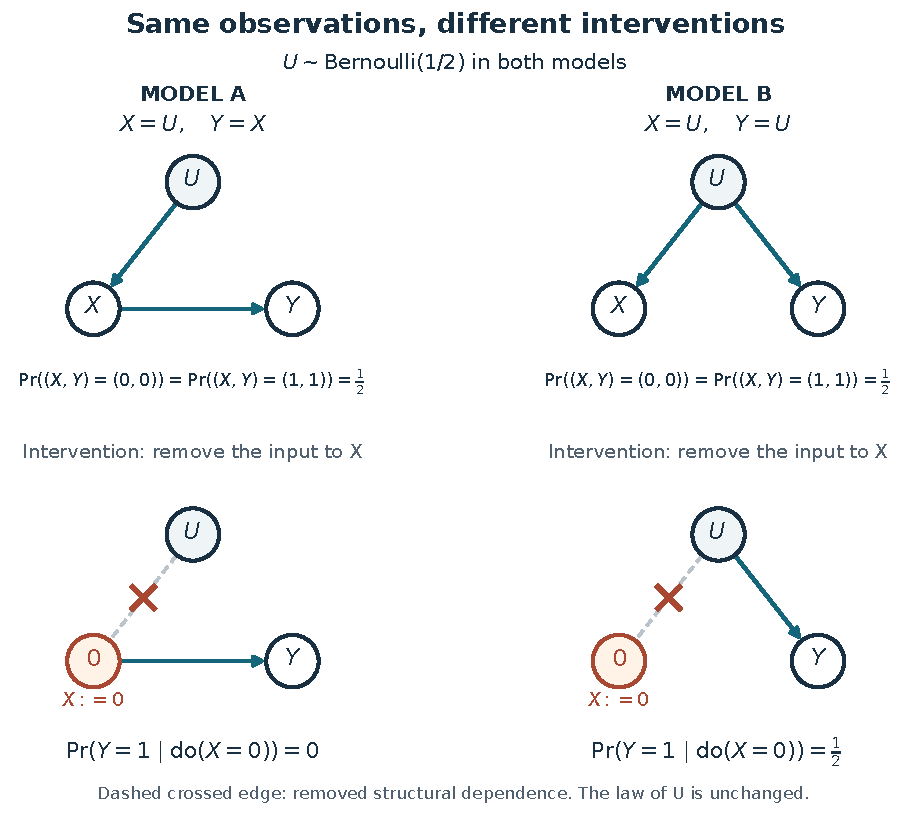
\includegraphics[width=\textwidth]{figures/second-pass-causal-models.pdf}
\caption{The same observational distribution does not identify a causal mechanism. Intervening on $X$ removes its incoming arrow. The two resulting laws for $Y$ differ even though the original observed $(X,Y)$ laws coincide.}
\label{fig:second-pass-causal}
\end{figure}

This impossibility applies equally to symbolic, neural, quantum, and human procedures with only those observations. It is an information limitation, not a defect peculiar to neural networks. Additional interventions, justified structural assumptions, or other observations can distinguish the models. The cosmology chapter uses precisely the same logic: a learned decoder cannot establish intentional cross-aeon communication if the proposed message and null hypotheses induce the same distribution on accessible observations.

The theorem also supplies a useful interpretation of ``understanding'' for this project. A system demonstrates a specified \emph{operational semantic competence} when it implements a model's interpretation map and answers its permitted transformations and counterfactual queries correctly. That is a testable property, with counterexamples and certificates. It does not settle phenomenal consciousness, the full semantics of natural language, or whether the supplied causal model is true of the world. Calling every such successful computation ``mere pattern matching'' adds no mathematical objection to its correctness.

\section{Empirical linguistic evidence and its strongest objection}

Gulordava and colleagues test long-distance agreement using semantically anomalous sentences and multiple languages, finding systematic syntactic generalization in recurrent language models \cite{LLgulordava}. Lakretz and colleagues identify internal units and circuits involved in number agreement and syntactic control \cite{LLlakretz}. These studies do not prove unlimited grammar mastery. They do provide concrete mechanisms and controlled behavior against which an assertion of exclusively superficial matching can be assessed.

Kallini and colleagues train GPT-2 variants on systematic transformations of English and observe differences in learning across their constructed languages \cite{LLkallini}. Their experiment challenges an unrestricted prediction of equal learning behavior. Hunter's subsequent critique identifies a serious confound: a central comparison adds a count-based nonadjacent dependency to one condition while leaving the other adjacent, instead of matching count-based and constituency-based nonadjacent dependencies \cite{LLhunter}. The experiment therefore does not settle whether the model's biases coincide with human grammatical constraints. Both findings belong in the assessment.

Comparisons between humans and language models also depend on the evaluation protocol. Lakretz and colleagues report a failure on particular long embedded dependencies \cite{LLnested}; Lampinen finds materially different performance when models receive prompts more comparable to the preparation supplied to human participants \cite{LLlampinen}. The appropriate conclusion is that instructions, examples, training distribution, and measured dependency type must be controlled. A benchmark failure is useful evidence about a defined setup. It is not an architecture-independent impossibility theorem.

For a stronger next experiment, construct pairs of synthetic grammars from one underlying set of annotated trees. Match vocabulary, sentence length, dependency distance, noise, and the number of extra transformation rules. Vary the grammatical relation of interest while keeping the nuisance quantities fixed or explicitly stratified. Train several architectures under matched data and optimization budgets; evaluate disjoint depths, vocabulary combinations, and intervention types. Compare test cross-entropy after accounting for the entropy of each data-generating process. Report counterexamples and uncertainty by stratum. This is a proposed experiment, not a result the present three-qubit graph benchmark has already established.

The hard counterstance does not require treating the weaker experiment as decisive. Chomsky's universal claim must itself meet a scientific burden. Demonstrated limitations and unresolved comparisons justify specific criticisms. They do not establish that neural models are permanently barred from representing mechanisms, learning useful linguistic structure, or contributing to explanations. Requiring an exact human developmental theory from every useful neural experiment mistakes one scientific question for all scientific questions about language.

\section{Learning a rule selector without surrendering guarantees}

Let $\mathcal R(G)$ be the finite set of certified grammar rules applicable to graph $G$. A model produces a probability distribution over this set. Its job may be to reduce a circuit's gate count, choose a template, propose a path, or select the next proof step. We can improve this proposal distribution while preserving a separate invariant checker. In particular, correctness of accepted semantic rewrites is independent of how they were ranked.

\begin{proposition}[A learned policy inherits certified rewrite correctness]
Suppose a system starts at a well-typed diagram, chooses any applicable rule according to an arbitrary, possibly history-dependent policy, checks the rule's stated semantic certificate, and accepts only certified rewrites. Every finite accepted run denotes the same map as its initial diagram.
\end{proposition}
\begin{proof}
Condition on any realized run. Each accepted step is a sound contextual replacement by Theorem~\ref{thm:typed-rewrite-soundness}. Induction on the finite number of accepted steps gives equal denotations. The policy's probabilities and parameters do not enter the argument.
\end{proof}

This is a substantive interface between learned and symbolic methods. The network can improve search order, while the checker enforces a property stated in mathematical terms. It does not make the checker unnecessary, and it does not make the learned component unimportant. Search cost can dominate a problem even when checking one proposed answer is easy. Whether a particular learned policy actually reduces that cost must be measured against a strong baseline with the same certificate budget.

For a quantum feature model, let $U_\theta(x)$ prepare a state and let $O_j$ be specified observables. Its classical feature vector has coordinates
$f_{\theta,j}(x)=\langle0|U_\theta(x)^\dagger O_jU_\theta(x)|0\rangle$.
These expectations are functions with a physical sampling cost and, for small circuits, an efficient classical implementation. A downstream model can use them to score graph rules. The model is therefore quantum in its feature construction when executed on quantum hardware, or a simulation of that construction when executed by cuQuantum or a CPU. A GPU state-vector simulation is a classical computation of a quantum model; this distinction is retained in the benchmark report.

\section{Finite-family generalization with an explicit selection cost}

A grammar can also generate candidate predictors. This introduces a statistical selection effect even if every candidate is mathematically well-typed. A small proof makes the cost visible.

\begin{lemma}[Bounded-variable exponential bound]
If $X\in[0,1]$ almost surely and $\mu=\mathbb EX$, then
$\mathbb E e^{\lambda(X-\mu)}\le e^{\lambda^2/8}$ for all real $\lambda$.
\end{lemma}
\begin{proof}
Let $\psi(\lambda)=\log\mathbb Ee^{\lambda X}$. Boundedness permits differentiation. Its second derivative is the variance of $X$ under the exponentially tilted probability measure. Any probability law supported on $[0,1]$ satisfies
$\operatorname{Var}(X)=\min_a\mathbb E(X-a)^2\le\mathbb E(X-1/2)^2\le1/4$.
Thus $\psi''\le1/4$, while $\psi(0)=0$ and $\psi'(0)=\mu$. Integrating this bound twice, or applying Taylor's theorem with integral remainder on the interval between zero and $\lambda$, gives
$\psi(\lambda)-\lambda\mu\le\lambda^2/8$.
\end{proof}

\begin{theorem}[Uniform error for a finite candidate family]
Let $K,m\ge1$ be integers and let $f_1,\ldots,f_K$ be predictors fixed independently of an independent identically distributed evaluation sample of size $m$. Let the loss lie in $[0,1]$, let $R_k$ be its population mean and $\widehat R_k$ its sample mean. For $0<\delta<1$, with probability at least $1-\delta$,
\[
 \max_{1\le k\le K}|\widehat R_k-R_k|
 \le \sqrt{\frac{\log(2K/\delta)}{2m}}.
\]
On this event the empirical minimizer's true risk is at most the best candidate's true risk plus twice this bound.
\end{theorem}
\begin{proof}
Independence and the exponential bound give
\[
 \mathbb E\exp\!\left(\lambda\sum_{i=1}^m(X_i-\mu)\right)
 \le\exp(m\lambda^2/8).
\]
Markov's inequality implies
$\Pr(\widehat\mu-\mu\ge\epsilon)\le\exp(-\lambda m\epsilon+m\lambda^2/8)$.
For $\lambda=4\epsilon$ this is $e^{-2m\epsilon^2}$; applying the same argument to $1-X$ gives the lower tail. A union bound over $K$ candidates yields $2K e^{-2m\epsilon^2}$. Solving for $\epsilon$ proves the displayed confidence bound. If $\hat k$ minimizes sample risk and $k_*$ minimizes true risk, then
$R_{\hat k}\le\widehat R_{\hat k}+\epsilon
\le\widehat R_{k_*}+\epsilon\le R_{k_*}+2\epsilon$.
\end{proof}

The independence condition matters. If the same evaluation data are repeatedly used to invent new predictors, the displayed proof no longer applies with the originally declared $K$. A finite family generated from a separate training sample can be conditioned on that sample and then evaluated on a fresh sample. More general adaptive selection requires another argument or a genuinely untouched final evaluation set. The cosmology chapter's global-null calibration addresses the analogous search over sky positions, template scales, and learned scoring rules.

This theorem does not certify the three-seed experiment merely because three is finite: the predictors are trained and selected, and their measured losses, splits, and boundedness must match its hypotheses. It supplies a reusable design rule. The reported benchmark uses explicit disjoint splits and exposes every seed; the finite-family theorem explains why tuning and final evaluation should be separated.

\section{What follows for the proposed cosmological grammar}

There are three layers in the proposed application. A physical model specifies how source degrees of freedom evolve through a crossover and into observable fields. A tensor grammar parameterizes candidate structures or messages consistent with that model. A learned function ranks or decodes those candidates using observed data. The second and third layers cannot establish the first by definition. They can make a specified physical hypothesis more testable.

One productive version is a restricted grammar of localized templates on an observed sky graph, with tensor-valued features for temperature, polarization, and angular correlations. A quantum feature map can feed an invariant graph scorer; a classical matched-filter or likelihood model supplies a strong baseline. The grammar's interface width determines a contraction budget. Null simulations must include the same mask, noise, foreground model, search over positions and widths, and learned model-selection procedure. Only held-out predictive success can establish that the search detected the stipulated class of signal better than its baseline. Attribution to a deliberate sender requires further, independently testable encoding structure.

At the logical level, the language of possible encoded messages can be regular, context free, or computationally more expressive depending on its stipulated encoder. Physics does not choose a Chomsky class merely by being quantum. A finite observed sky gives a finite dataset; an asymptotic language classification concerns a family of encoders and increasingly large observations. These are related through a specified model, not through the word ``information'' alone.

The same reasoning sharpens the reply to Chomsky. A neural system can participate in a disciplined semantic pipeline, can implement recursive and counterfactual algorithms, and can be evaluated on transformations that expose what it has learned. Demanding those tests is good science. Declaring the entire approach incapable of understanding in principle is not a consequence of the mathematical hierarchy, and is contradicted as a broad computational prohibition by the explicit constructions above. The unresolved question is which trained systems acquire which mechanisms, at what data and computational cost, with what robustness. That is an empirical and mathematical research program, not a reason to dismiss the program before doing it.

\chapter{A worked bridge: orders, periodic complexes and spectra}
\label{ch:worked-bridge}

The preceding chapters provide several legitimate connections, each with a
specified domain of validity. We now place them beside one another in a single
calculation. Its purpose is to identify exactly which structures survive a
change of viewpoint. The example is elementary enough to calculate without
appealing to an existence theorem, but rich enough to distinguish a generic
semisimple algebra, an integral order, a singular special fiber, an infinite
projective resolution, and a positive finite-dimensional Hodge operator. It
also directly uses the nodal order occurring in the inherited research
program \citep{GRHRepo,SchreiberSurfaceI,SchreiberSurfaceII}.

\section{The order and its two complementary elements}

Let $R$ be a commutative integral domain, let $u\in R$ be nonzero, and set
\[
 \Lambda=R[X]/(X^2-uX),\qquad x=\overline X,\qquad y=u-x.
\]
Then $xy=yx=0$. The polynomial is monic, so every element of $\Lambda$ has a
unique expression $a+bx$, with $a,b\in R$. Relative to the basis $(1,x)$,
multiplication by $x$ and $y$ is represented by
\[
 M_x=\begin{pmatrix}0&0\\1&u\end{pmatrix},\qquad
 M_y=\begin{pmatrix}u&0\\-1&0\end{pmatrix}.
\]
These matrices exhibit the zero-composition condition as an identity over the
coefficient ring, before any choice of scalar field or inner product.

\begin{proposition}[An exact periodic complex]\label{prop:periodic-order}
There is an exact complex of free $\Lambda$-modules
\[
 \cdots\xrightarrow{x}\Lambda\xrightarrow{y}\Lambda
 \xrightarrow{x}\Lambda\xrightarrow{y}\Lambda\xrightarrow{x}\cdots.
\]
Here an arrow labelled by an element denotes multiplication by that element.
Moreover, with $M=\Lambda/x\Lambda$, the augmented sequence
\[
 \cdots\xrightarrow{x}\Lambda\xrightarrow{y}\Lambda
 \xrightarrow{x}\Lambda\longrightarrow M\longrightarrow0
\]
is a free resolution of $M$.
\end{proposition}
\begin{proof}
For $a+bx\in\Lambda$,
\[
 x(a+bx)=(a+ub)x,\qquad y(a+bx)=a(u-x)=ay.
\]
Uniqueness of the basis expansion gives
\[
 \ker M_x=R(x-u)=Ry,\qquad \im M_y=Ry.
\]
It also gives $\ker M_y=Rx$: the coefficient of $x$ in $ay$ is $-a$, so
$ay=0$ implies $a=0$. Finally $\im M_x=Rx$, since $x=x\cdot1$. Thus the
kernel of each arrow is the image of the preceding one. The quotient map
onto $M$ has kernel $x\Lambda=Rx$, which verifies exactness at the augmented
term. Every unaugmented term is the free module $\Lambda$ of rank one.
\end{proof}

The ring need not be a domain: indeed $xy=0$. This is not a defect in the
argument. The coefficient ring $R$ is a domain, whereas the order $\Lambda$
is a ring with zero divisors. Keeping those two statements separate prevents
an erroneous cancellation of $x$ or $y$. In particular, this is not a
regular-sequence Koszul resolution. It is a periodic resolution arising from
the explicit annihilator identities.

\section{Tensor products detect information that ranks omit}

The module $M$ is isomorphic to $R$ as an $R$-module, with $x$ acting as zero.
The action of $y$ on $M$ is consequently multiplication by $u$. Tensoring the
resolution with $M$ over $\Lambda$ produces the chain complex
\[
 \cdots\xrightarrow{0}R\xrightarrow{u}R
 \xrightarrow{0}R\xrightarrow{u}R\xrightarrow{0}R.
\]
The rightmost copy is in degree zero.

\begin{proposition}[An explicit derived obstruction]\label{prop:tor-node}
For $M=\Lambda/(x)$ as above,
\[
 \Tor^{\Lambda}_{2j+1}(M,M)\cong R/uR\quad(j\geq0),
 \qquad
 \Tor^{\Lambda}_{2j}(M,M)=0\quad(j\geq1).
\]
In degree zero $M\otimes_\Lambda M\cong R$.
\end{proposition}
\begin{proof}
The displayed free resolution computes the derived tensor product. Its odd
differentials are zero, and its positive even differentials are
multiplication by $u$. Since $R$ is a domain and $u\ne0$, the latter maps are
injective. The homology in positive even degree is therefore zero. In odd
degree the kernel is all of $R$ and the incoming image is $uR$, giving
$R/uR$. In degree zero the incoming differential is zero. This establishes
all the assertions directly from the definition of homology.
\end{proof}

If $u$ is a unit, the positive Tor groups vanish, and the generic splitting
is already available over $R$. If $u$ is a nonunit, the odd groups record a
defect supported on its vanishing locus. Their $R$-rank is zero, so taking
generic ranks erases this information completely. This is a concrete reason
to retain the exact category of lattices and derived functors when comparing
orders. A rational representation and its integral model can agree in rank
while disagreeing substantially in extension theory.

This example also guards against a misleading computational inference.
Efficient manipulation of the two small matrices computes this particular
resolution. It says nothing about a polynomial-time procedure for arbitrary
module classification, arbitrary syzygies, or a cryptographic search problem.
The presentation size, coefficient bit lengths, and demanded output are part
of any complexity statement.

\section{Generic splitting and singular specialization}

Over the fraction field $K$ of $R$, the two elements
\[
 e_x=x/u,\qquad e_y=y/u
\]
are orthogonal idempotents with $e_x+e_y=1$. Thus
$K\otimes_R\Lambda\cong K\times K$. The denominators matter: if $u$ is not
invertible in $R$, these idempotents need not belong to $\Lambda$ itself.
The generic decomposition therefore need not be an integral decomposition.
This is the same elementary obstruction that appears when an overorder
introduces idempotents unavailable in the smaller order.

For $R=k[u]$ or $k[[u]]$, reduction modulo $u$ gives
\[
 \Lambda/u\Lambda\cong k[X]/(X^2).
\]
The special fiber has a nonzero nilpotent, whereas the generic fiber is a
product of fields. The periodic maps reduce to multiplication by $X$ and
$-X$, whose image and kernel both equal $kX$. Thus exactness survives this
particular reduction. This conclusion follows from an explicit calculation;
it must not be generalized to a statement that every exact complex remains
exact after arbitrary nonflat base change. Proposition~\ref{prop:tor-node}
already demonstrates the contrary phenomenon for another tensor operation.

\section{The finite Hodge operator of the same complex}

We next work over $\R$ and evaluate the parameter at a real number $t$.
This is a finite matrix family. Equip every copy of $\R^2$ with the standard
Euclidean inner product, and take the consecutive differentials
\[
 A_t=\begin{pmatrix}0&0\\1&t\end{pmatrix},\qquad
 B_t=\begin{pmatrix}t&0\\-1&0\end{pmatrix}.
\]
Their composite vanishes for every $t$, and each matrix has rank one.
The middle Hodge Laplacian is
\[
 \Delta_t=A_tA_t^T+B_t^TB_t.
\]

\begin{proposition}[Exactness and an explicit metric gap]
For every $t\in\R$,
\[
 \Delta_t=(1+t^2)I_2.
\]
Its kernel is zero and its least eigenvalue is $1+t^2\geq1$.
For every $\eta>0$, replacing both differentials by
$\eta A_t,\eta B_t$ preserves their images, kernels and exactness but
replaces the Laplacian by $\eta^2(1+t^2)I_2$.
\end{proposition}
\begin{proof}
Direct multiplication gives
\[
 A_tA_t^T=\begin{pmatrix}0&0\\0&1+t^2\end{pmatrix},\qquad
 B_t^TB_t=\begin{pmatrix}1+t^2&0\\0&0\end{pmatrix}.
\]
Adding proves the identity. A scalar multiple of the identity has the stated
eigenvalues. Multiplication of a linear map by a nonzero scalar changes
neither its image nor its kernel. Its contribution to $AA^T+B^TB$ is
multiplied by the square of that scalar, which proves the final assertion.
\end{proof}

Several lessons are visible simultaneously. A singular algebraic fiber does
not force this chosen finite Hodge gap to close. Conversely, exactness and
the same algebraic rank stratum do not provide a positive lower bound when
the scale of the differential is allowed to vary. The inner product and
normalization of the operator are essential data. The latter statement is
the finite counterpart of the much larger distinction between a topological
index and a uniform physical spectral gap. It supplies a counterexample to
an inference; it does not model the interacting Yang--Mills Hamiltonian.

\section{How the cryptographic comparison enters}

The derived obstruction $R/uR$ and the cyclic hidden subgroup in the
cryptography chapter are both quotients of explicitly presented modules.
That common language is useful: one can write maps, calculate kernels and
compare exact sequences. Their computational roles are nevertheless
different. A presentation of $R/uR$ includes its relation $u$. In an elliptic
curve discrete logarithm instance $Q=dP$, the unknown $d$ is precisely the
parameter of the hidden kernel
\[
 H_d=\{(-dt,t):t\in\Z/q\Z\}.
\]
Writing $H_d$ symbolically does not compute $d$. Fourier sampling obtains
information about its annihilator using a quantum evaluation procedure for
the public map $(a,b)\mapsto aP+bQ$. A useful algorithmic bridge must explain
how representations of the relevant maps are obtained without first solving
the hidden problem.

Similarly, writing down a lattice basis after knowing a secret scalar is not
a reduction from an unknown scalar to lattice reduction. The basis of the
endomorphism relation lattice in the cryptography chapter is available when
the action of the specified endomorphism on the cyclic subgroup is known.
That availability is an input condition. The abstract existence of an
endomorphism in an order does not automatically provide its efficient
evaluation, its scalar action on a selected subgroup, or a short basis in a
specified metric.

\chapter{A quantitative synthesis and a research program}

\section{The information that each theory actually supplies}

The most useful common objects are modules with extra structure and complexes
of maps between them. The relevant extra structure changes from chapter to
chapter. An order-lattice is an integral module inside a rational
representation. A cryptographic lattice is supplied with a norm,
representation and probability distribution. An elliptic complex is supplied
with differential operators and an exact principal-symbol sequence away from
the zero section. A quantum theory is supplied with positive correlation
functionals, spacetime covariance, locality and a reconstruction procedure.

These additions are not optional embellishments to an otherwise complete
algebraic answer. They determine which questions are meaningful. The matrix
equation $BA=0$ determines a variety of complexes, but no quantum resource
cost. A $K$-theory class determines the stable topological input to an index
pairing, but no absolute time scale. A free abelian group determines neither
the length of a shortest vector nor the distribution of a sampled error.

\begin{longtable}{p{.20\textwidth}p{.33\textwidth}p{.37\textwidth}}
\toprule
Interface & Data retained & Additional data needed for the next question\\
\midrule\endhead
Order to rational algebra & Scalar extension, representation, rank & Integral
conductor, local structure and lattice class\\
Order to geometric lattice & An embedding into a real vector space & Positive
form, basis, coefficient sizes and distortion bounds\\
Complex to cohomology & Kernel modulo image & Chosen inner products and
quantitative singular values\\
Elliptic symbol to index & Symbol $K$-class and characteristic pairing & Domains,
boundary conditions and estimates on positive spectrum\\
Group action to quantum algorithm & An abstract operation or oracle & Reversible
implementation, cleanup, precision and total resource accounting\\
Lattice action to LWE problem & Module arithmetic & Error law, parameter regime,
sample distribution and a reduction\\
Euclidean correlations to a QFT & Positive continuum functionals and axioms &
Control of phases, quantitative large-distance decay and spectral support\\
\bottomrule
\end{longtable}

The table organizes a rigorous synthesis because each row is an interface
with testable requirements. It prevents a conclusion from one category being
silently reinterpreted as a conclusion in another.

\section{A general comparison estimate}

There is a simple quantitative principle behind several of these interfaces.
Let $V$ be a finite-dimensional real inner-product space, let $\Delta$ be a
positive semidefinite self-adjoint operator, and suppose its kernel is $K$.
A gap statement is a lower bound on the orthogonal complement of $K$:
\[
 \langle v,\Delta v\rangle\geq c\|v\|^2\qquad(v\perp K).
\]
Algebraic identifications transport vectors. To transport this inequality,
they must also control norms and quadratic forms.

\begin{proposition}[Transport of a coercivity bound]
Let $V,W$ be finite-dimensional real inner-product spaces, $T:W\to V$ a
linear isomorphism, and $q$ a nonnegative quadratic form on $V$ with kernel
$K$. Suppose
\[
 q(v)\geq c\,\operatorname{dist}(v,K)^2\quad(v\in V),
 \qquad \|Tw\|\geq m\|w\|\quad(w\in W)
\]
with $c,m>0$. Put $q_T(w)=q(Tw)$ and $K_T=T^{-1}K$. Then
\[
 q_T(w)\geq cm^2\,\operatorname{dist}(w,K_T)^2.
\]
\end{proposition}
\begin{proof}
For every $k\in K$, write $k=Tz$ with $z\in K_T$. Then
$\|Tw-k\|=\|T(w-z)\|\geq m\|w-z\|$. Taking the infimum over $k$, equivalently
over $z$, gives
$\operatorname{dist}(Tw,K)\geq m\operatorname{dist}(w,K_T)$.
Apply the assumed bound for $q$ and square the latter inequality.
\end{proof}

This estimate has deliberately modest scope. It does not construct $T$, prove
that $m$ stays away from zero in a limit, or identify a finite matrix with a
physical Hamiltonian. It shows exactly what must be added to an algebraic
identification to transport a lower spectral bound. The same smallest
singular value controls distortion of short vectors in a lattice. The same
absence of a uniform bound can invalidate a proposed continuum-limit argument
or a proposed cryptographic reduction.

\begin{corollary}[Why pointwise equivalence is insufficient]
For a family of isomorphisms $T_j$, positive constants $m_j$ for each fixed
$j$ do not imply a uniform positive lower bound for the transported quadratic
forms. On $V=W=\mathbb R$, with $j\ge1$ and $q(v)=\|v\|^2$,
the choice $T_j=j^{-1}I$ gives
$q_{T_j}(w)=j^{-2}\|w\|^2$.
\end{corollary}
\begin{proof}
The displayed identity follows from homogeneity of the norm. Its least
Rayleigh quotient is $j^{-2}$, which tends to zero. Each $T_j$ remains an
isomorphism.
\end{proof}

\section{A diagram with explicit logical boundaries}

There is a defensible route from the two books to the other topics. Integral
orders organize endomorphism rings and modules. These produce complexes and
deformation problems, whose finite algebra can be studied through rank
strata. Smooth geometric counterparts have symbol complexes and index
classes. Gauge theory supplies a particularly important elliptic deformation
complex. Finite abelian groups and modules also support the character theory
underlying quantum hidden-subgroup algorithms. The links are structural and,
in examples such as the preceding chapter, computationally explicit.

What is absent is a theorem making the path transitive at the level of the
most difficult conclusions. An endomorphism order does not turn an ASD index
into an ECC discrete logarithm algorithm. A positive finite Hodge Laplacian
does not establish a uniform infinite-volume Yang--Mills gap. A functional
equation and real coefficients do not identify an arithmetic determinant
with a self-adjoint operator. These omissions are the mathematical content of
the remaining research questions, rather than details to be supplied by an
unlabelled analogy.

\section{Three concrete research directions}

\subsection{Arithmetic modules with explicit metric control}

A productive first direction is to choose a family of orders and record,
together, its integral presentation, archimedean embeddings, positive form,
local conductor, and a basis with certified coefficient sizes. The codifferent
calculation in the cryptography chapter provides the correct dual object
under a trace pairing. The shear example shows why a module isomorphism alone
cannot certify a short-vector comparison. A useful theorem would provide a
uniform, explicit distortion bound for a specified family of transformations,
with the bound expressed in the same parameter as the input bit length.

For an imaginary quadratic order, one can begin with explicit ideal lattices
and the complex absolute-value metric. One must state which ideals are
invertible, whether the order is maximal, how the discriminant varies, and
which basis or reduced representative is produced. These restrictions are
essential for a valid theorem about dual ideals or norm comparison. Extending
such a theorem to noncommutative orders requires specifying left versus right
modules and the chosen involution or positive representation.

The computational companion provides small exact examples, not an asymptotic
complexity result. A subsequent study should measure both coefficient growth
and geometric distortion. Reporting only a favorable rank or module
decomposition would leave the main quantitative issue unanswered.

\subsection{Resource-certified elliptic-curve quantum arithmetic}

The reproducibility program is implemented in the companion's
\texttt{workbench/program3/ecc.py}, with separate emitted variable-point
addition oracles, independent gate counting and clean-work verification.
The current continuation, \emph{Arithmetic, Coverings and Learned Quantum
Renormalization}, gives the construction, proofs, tested resource comparisons
and observational controls. Historical editions retain the original research
direction; this source records its implemented successor.

The comparison fixes nonsingular finite curves, affine coordinates with a
unique infinity encoding, invalid-word behavior, ideal X/CX/CCX gates and
ancillary-register initialization. Both the binary path and coherent signed
endomorphism decomposition include every preparation and cleanup operation.
Finite exhaustive-domain checks and actual cuStateVec replay are recorded at
their precise scope. The bounded truth-table compiler is not a polynomial-size
implementation for cryptographic curves, and logical counts are not
error-corrected physical resource estimates.

In the tested instances, decomposition does not reduce the complete budget.
The emitted circuits make that result reproducible instead of inferring a
saving from shorter scalar components alone. The independent source, circuit
streams, assumption manifest and verification reports accompany the versioned
continuation. Its hierarchical channel and covering-theory extensions preserve
the distinction between an arithmetic endomorphism, a quantum channel, a graph
cover and a learned renormalization map.

\subsection{From elliptic estimates to a uniform physical gap}

A third direction begins with the Yang--Mills existence framework reviewed in
this manuscript. The independent assessment separates existence from the
mass-gap problem \citep{YMReview2026}. A further theorem needs a quantitative
bound strong enough to survive ultraviolet and infinite-volume limiting
procedures, together with a correct identification of the reconstructed
observables and vacuum sector.

The spectral theorem argument in the gauge chapter gives a precise target:
uniform exponential decay on the orthogonal complement of the vacuum is
equivalent to a positive lower spectral threshold, with the stated domain
and cyclicity conditions. The UV counterexample there proves that matching
leading short-distance behavior cannot alone establish this target. A new
mass-gap argument must therefore add infrared information. The ASD index
formula may organize classical deformation spaces, but it does not provide
the required estimate for the interacting quantum Hamiltonian.

Formalization could assist by making the limiting and reconstruction
interfaces explicit. The hard step would remain a proved analytic estimate,
not a declaration naming a gap constant. A sound Lean statement must quantify
over the relevant cutoffs and volumes, give the correct normalization, and
make positivity of the common lower bound an actual conclusion or a clearly
identified hypothesis. The formalization appendix explains this distinction
using smaller declarations that can be compiled in the present project.

\section{What this monograph establishes}

This work supplies a coherent collection of explicit constructions,
elementary proofs, counterexamples to invalid transfers, a source audit,
selected machine-checked algebra, and reproducible finite experiments. It
does not assert a proof of GRH, a Yang--Mills mass gap, a generally faster ECC
algorithm, or a new security reduction for lattice cryptography. Those would
require additional theorems not contained in the source material or proved
here.

The strongest common principle obtained from the comparison is quantitative:
an algebraic or categorical connection becomes an algorithmic or spectral
connection only after its representations, metrics, probability laws,
normalizations and limiting operations are controlled. The examples make
each part of that principle testable. The research directions above specify
what a successful next theorem would have to say and what evidence would
make it independently assessable.

\appendix
\chapter{Reproducible finite experiments and interactive geometry}

\section{What the computations verify}

The computational companion has two independent implementations of the
principal finite examples: Python for the paper's exact checks and figures,
and JavaScript for the interactive page. Both are deliberately small. Their
purpose is to make definitions inspectable, expose exceptional cases, and
check consistency between formulas and displays. Neither is an implementation
of production cryptography or a simulator of continuum Yang--Mills theory.

The Python script \path{code/verify_examples.py} uses only the standard
library.

It writes \path{verification/examples.json}, including a SHA-256
hash of the script, exact finite counts, and numerical residuals. The figure
script additionally uses NumPy and Matplotlib. The browser experiments are
buildless and use no remote JavaScript dependency. A separate Node script
\path{site/verify-math.cjs} checks the shared mathematical functions used
by the interface. The environment and invocation commands are recorded in
the project README.

It is important to distinguish three kinds of evidence. A symbolic proof
establishes an identity for all objects under its assumptions. Exhaustive
finite enumeration establishes a property of the enumerated finite
structure. A floating-point residual checks a sampled numerical
implementation up to a tolerance. The companion labels these categories
explicitly. For example, checking $BA=0$ to $10^{-12}$ at sample points on a
projected cone is not a proof of exactness, and a table of 19 elliptic-curve
points is not a proof of the group law for every elliptic curve.

\section{The 19-element elliptic-curve example}

The curve
\[
 E:\quad y^2=x^3+2x+2\quad\text{over }\F_{17}
\]
has 18 affine points and one point $O$ at infinity. The enumeration checks
every pair $(x,y)\in\F_{17}^2$ directly. It also checks that
$P=(5,1)$ has order 19 and generates the entire set. The affine formulas
treat the identity, inverse pairs and tangent cases separately. This is
essential: blindly inverting a zero denominator would invalidate the
implementation.

\begin{center}
\begin{tabular}{rrrr}
\toprule
$k$ & $kP$ & $k$ & $kP$\\
\midrule
0 & $O$ & 10 & $(7,11)$\\
1 & $(5,1)$ & 11 & $(13,10)$\\
2 & $(6,3)$ & 12 & $(0,11)$\\
3 & $(10,6)$ & 13 & $(16,4)$\\
4 & $(3,1)$ & 14 & $(9,1)$\\
5 & $(9,16)$ & 15 & $(3,16)$\\
6 & $(16,13)$ & 16 & $(10,11)$\\
7 & $(0,6)$ & 17 & $(6,14)$\\
8 & $(13,7)$ & 18 & $(5,16)$\\
9 & $(7,6)$ & 19 & $O$\\
\bottomrule
\end{tabular}
\end{center}

The exact test enumerates all $19^3=6,859$ triples and checks associativity
with modular integer arithmetic. It checks closure and commutativity on all
pairs. Finally, for each of the 19 choices of $d$, it enumerates the kernel of
$(a,b)\mapsto aP+b(dP)$ and compares it to
$\{(-dt,t):t\in\Z/19\Z\}$. This last comparison connects the concrete curve
display to the hidden-subgroup theorem in the text.

\begin{figure}[htbp]
\centering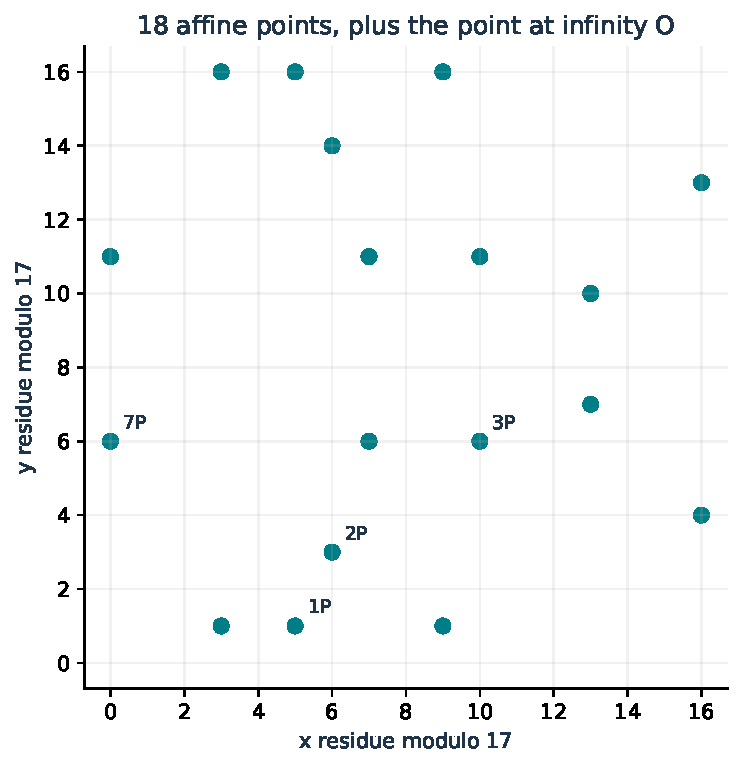
\includegraphics[width=.80\textwidth]{figures/ecc17.pdf}
\caption{The finite-field curve is a discrete set of residues. The straight
layout of the residue grid is a display convention; it is not the real
plane cubic, and Euclidean distances between the plotted dots have no role
in its group law. The point $O$ is handled separately.}
\end{figure}

The browser lets the reader select a scalar and see its corresponding point.
The small modulus makes every operation inspectable. It also makes this
example unsuitable as a security parameter: exhaustive enumeration is
intentional. The page does not accept real keys or provide an attack service.

\section{The Fourier annihilator experiment}

For the group $(\Z/7\Z)^2$ and $d=3$, the exact Fourier support is
\[
 (0,0),(1,3),(2,6),(3,2),(4,5),(5,1),(6,4).
\]
Each outcome has probability $1/7$. Every other grid point has probability
zero. The exact proof is the geometric-sum identity in the cryptography
chapter. The Python computation evaluates the complex exponential sum
numerically and compares its squared modulus with that exact probability
table. The discrepancy is recorded rather than rounded into a claim of
exact floating-point equality.

\begin{figure}[htbp]
\centering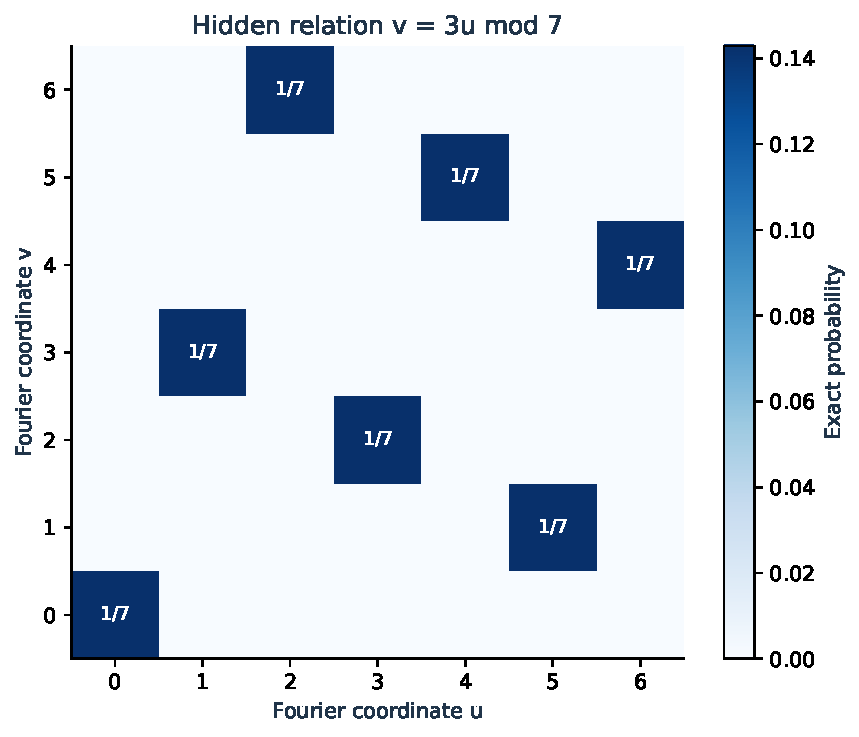
\includegraphics[width=.75\textwidth]{figures/fourier7.pdf}
\caption{Fourier mass lies on the annihilator $v=3u\pmod7$. The color bar
measures probability, not amplitude. Six of the seven possible outcomes
have nonzero $u$ and therefore recover $d$ by the stated modular inverse.}
\end{figure}

The interactive version varies the hidden slope $d$. The seven supported
points change accordingly, while the normalization remains one. This is a
finite mathematical simulation of the distribution. It does not simulate
the physical implementation of a quantum Fourier transform, and the page's
knowledge of $d$ is part of the demonstration setup. A real algorithm must
obtain its information from the oracle evaluations described in the proof.

\section{A genuine four-coordinate variety}

The variety of complexes of dimension vector $(1,2,1)$ has coordinates
\[
 A=\begin{pmatrix}x_1\\x_2\end{pmatrix},\qquad
 B=\begin{pmatrix}y_1&y_2\end{pmatrix},\qquad
 BA=x_1y_1+x_2y_2=0.
\]
The browser displays the real locus in $\R^4$. It does not identify this
four-real-dimensional ambient space with the complex variety's real
eight-dimensional ambient space. The real cone has dimension three away
from its vertex. Its unit-sphere link is two-dimensional.

Set
\[
 u=2^{-1/2}(\cos\alpha,\sin\alpha),\qquad
 v=2^{-1/2}(\cos\beta,\sin\beta),\qquad
 x=(u+v)/\sqrt2,\quad y=(u-v)/\sqrt2.
\]
Then
\[
 x\cdot y=\tfrac12(\|u\|^2-\|v\|^2)=0,
 \qquad \|x\|^2+\|y\|^2=\|u\|^2+\|v\|^2=1.
\]
The coordinate transformation is orthogonal and invertible. Its inverse
sends every point of the unit link to two vectors of norm $1/\sqrt2$.
Hence the link is $S^1\times S^1$. This derivation is the reason the
parameterization is used; a generic torus-shaped drawing would not establish
that it represents the intended algebraic set.

\begin{figure}[htbp]
\centering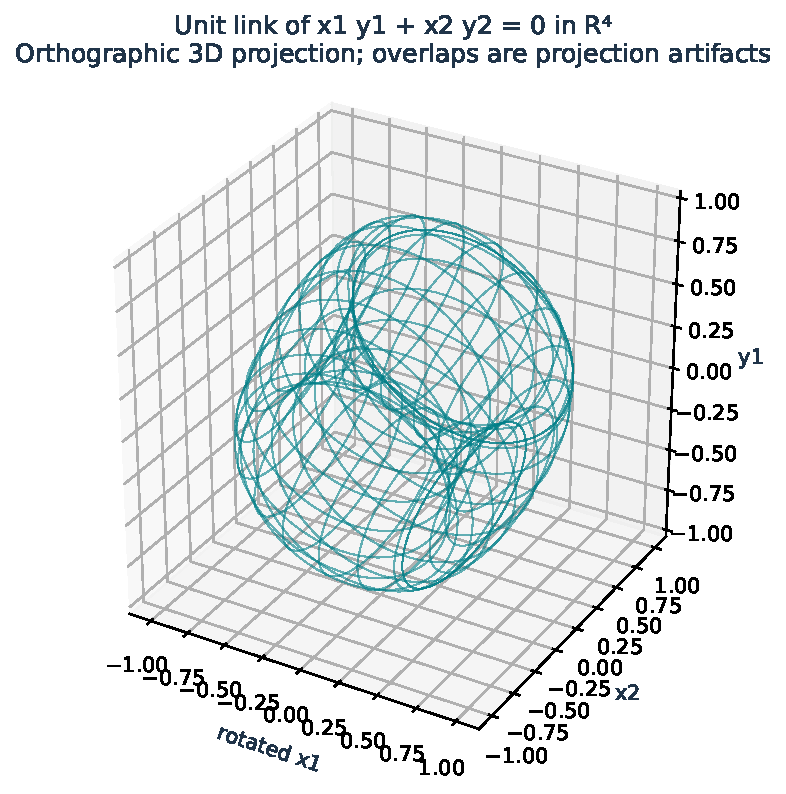
\includegraphics[width=.85\textwidth]{figures/cone_link.pdf}
\caption{A specified rotation in four-dimensional coordinate space followed
by orthographic projection into three dimensions. Apparent intersections
can be caused by projection. The mathematical link lies in $S^3\subset\R^4$;
it is not an embedded surface in ordinary three-dimensional space under
every projection.}
\end{figure}

The page exposes rotation and projection controls and reports the defining
equation's residual. Rank strata are derived from whether $A$ and $B$ vanish,
rather than inferred from the appearance of the projected image. The origin
is handled separately from the link. The tangent calculation is also
separate: a direction satisfying the linearized equation may retain a
quadratic obstruction, as proved and partially formalized in the companion.

\section{Index, kernel and gap are separate readouts}

For
\[
 A_\eps=(\eps,0)^T,\qquad B=(0,1),
\]
the middle Laplacian is $\diag(\eps^2,1)$. For $\eps\ne0$ the complex is exact
in the middle and its least eigenvalue is positive. As $\eps\to0$ the lowest
eigenvalue approaches zero. At $\eps=0$ the kernel dimension changes. The
Euler characteristic of the underlying three-term complex remains
$1-2+1=0$. At the endpoint, the smallest \emph{positive} eigenvalue is 1,
whereas the smallest eigenvalue is 0; these are different readouts and the
page distinguishes them.

\begin{figure}[htbp]
\centering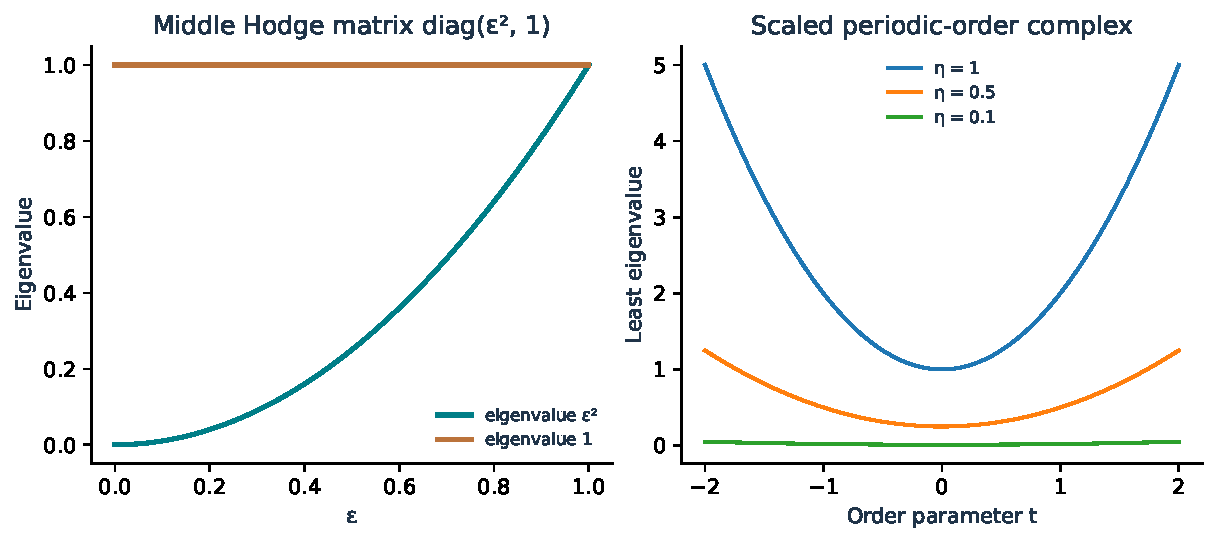
\includegraphics[width=\textwidth]{figures/hodge_gaps.pdf}
\caption{Left: a fixed Euler characteristic with changing kernel and lower
eigenvalue. Right: the exact periodic-order example has eigenvalue
$\eta^2(1+t^2)$ after rescaling both differentials. Algebraic exactness does
not determine a metric scale. These are finite matrices, not physical
Yang--Mills Hamiltonians.}
\end{figure}

The twisted flat-torus spectrum provides an infinite-dimensional counterpart
whose eigenvalues are still explicit. With $L_1=L_2=1$ and automorphy
parameters $(s,0)$ for $s\in[-1/2,1/2]$, its lowest scalar eigenvalue is
$4\pi^2s^2$. At the trivial character a zero mode appears. This plot belongs
to a free rank-one flat connection, and it must not be read as an interacting
nonabelian quantum mass-gap computation.

\begin{figure}[htbp]
\centering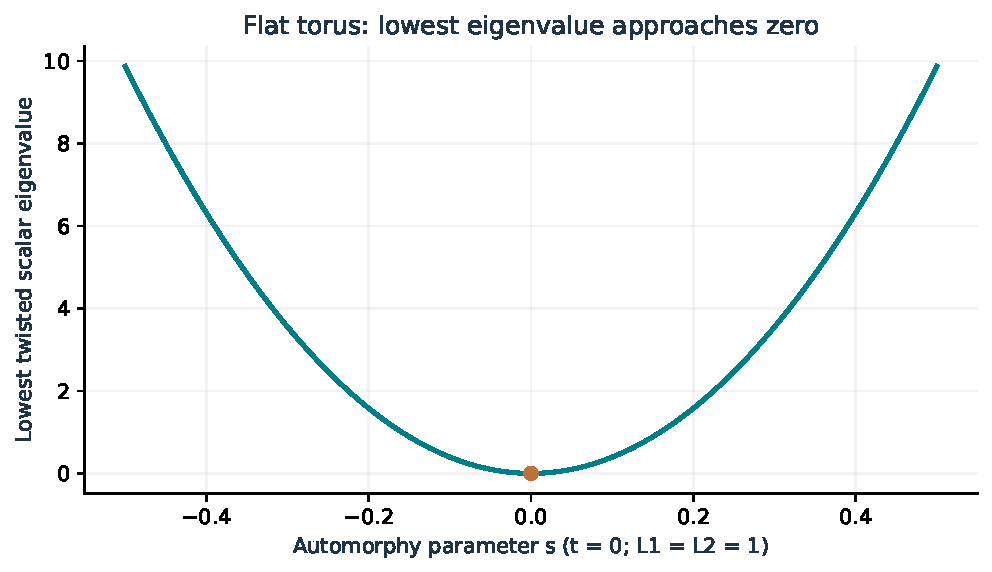
\includegraphics[width=.85\textwidth]{figures/twisted_gap.pdf}
\caption{An exact slice of the flat-torus spectral family. The horizontal
coordinate is an automorphy parameter modulo one; it is not time, energy,
or a lattice-spacing cutoff.}
\end{figure}

\section{The torus and plaquette displays}

The elliptic-torus laboratory starts with $\C/(\Z+\tau\Z)$, where
$\operatorname{Im}\tau>0$. A lattice Gram matrix records the flat metric of
the fundamental parallelogram. The familiar doughnut in three-dimensional
space is a topological visualization of the quotient, not an isometric
embedding of that flat metric. Changing $\tau$ changes the complex structure
and the displayed lattice data; an attractive three-dimensional surface
cannot substitute for those coordinates.

The optional gauge laboratory uses a single $U(1)$ plaquette. If edge
variables are $U_i$ and vertex transformations are $g_i$, then
\[
 U_i\longmapsto g_iU_ig_{i+1}^{-1}
\]
preserves the oriented product around the plaquette, since consecutive
factors cancel. For a nonabelian group the product is conjugated at the
base vertex and its trace is invariant. The browser displays the abelian
identity and a numerical residual. It does not generate a Yang--Mills
ensemble, take a continuum limit, or estimate a physical mass.

\section{Reproduction and interpretation}

The README gives commands for regenerating the JSON evidence and five
publication figures. Browser controls use native keyboard-accessible inputs;
the camera also supports keyboard rotation. Motion is user-controlled and
the reduced-motion preference is respected. Equations, parameter labels and
numeric summaries remain available alongside the canvas. The static
application uses relative links, so the same files can be served from a
local checkout or a project-hosting subdirectory.

Reproduction should begin with the small exact tests. If they fail, the
display should not be trusted. If they pass, that establishes consistency
for the tested examples, not every theorem in the paper. The next appendix
describes the different and stronger guarantee supplied by the selected
Lean declarations, together with the exact limits of that guarantee.

\section{Exact algebraic companion checks}
The gentle-invariant verification script checks all \(3^{10}=59{,}049\) ten-coordinate vectors with entries in \(\{0,1,2\}\), finds the 257 satisfying the four matching equations, and decomposes every one using the constructive proof. It also checks 100 larger constructed examples, the two corrected exponent relations, and 135 exact block determinants for the Kronecker pencil. Direct pair arithmetic in \(\F_{17}[u]/(u^2-3)\) counts 323 points on the companion elliptic curve, agreeing with the independently derived zeta recurrence. These results are recorded in \texttt{extension/verification/invariants.json}.

The interactive algebra companion has separate exact checks: 6,561 small Plucker matrices; all fifteen tableaux of shape \((3,2)\) on three letters; 2,478 admissible gentle rank cases, tested by independent elimination in characteristics two and seven; and 6,561 matching-generator monomials with 4,529 distinct exponent vectors. These finite tests verify implementations of the proved formulas; they are not substitutes for the unbounded proofs in the algebraic chapters.

The quantum companion and its GPU results are described in the quantum-surface chapter. The browser worker was also exercised through its actual controls: the 42-gate encoder produced support on 256 basis states with norm and all stabilizers equal to one to the displayed precision; an X error on edge zero flipped exactly the two adjacent face checks; and a live gradient update reduced the displayed loss with all sixteen predictions computed. Browser layout checks included a 375-pixel content viewport without page-level horizontal overflow.

\chapter{The Lean 4 companion: verified statements and explicit limits}

\section{Current six-module verification}

The current companion contains 115 selected theorem declarations in six
modules.
\begin{center}
\begin{tabular}{lr}
\toprule
Module & Declarations\\\midrule
\texttt{BridgeTheorems} & 25\\
\texttt{QuantumInterfaces} & 7\\
\texttt{DiagramGrammar} & 16\\
\texttt{FluidInterfaces} & 34\\
\texttt{ReductionContracts} & 16\\
\texttt{TransportContracts} & 17\\\bottomrule
\end{tabular}
\end{center}
The final verification records a fresh compiler check, exact printed types,
source hashes and axiom dependencies for every declaration, with no warnings
or unexpected axioms. Its authoritative record is
\texttt{lean/final-verification/verification.json} and the six module logs.
The formal type map identifies 68 declarations with precise partial
components of 25 manuscript environments; no whole composite environment is
labelled completely formalized. This verification covers the selected local
interfaces, not the full upstream continuum proof or cryptographic security.

The following section preserves the original 25-declaration module's exact
verification record, which remains a component of the current package.

\section{Original module verification result}

The file \texttt{lean/BridgeTheorems.lean} contains 25 named theorem
declarations. It was compiled successfully with Lean 4.24.0 on Linux, using
mathlib revision
\begin{center}\small\texttt{f897ebcf72cd16f89ab4577d0c826cd14afaafc7}.\end{center}
The compiler exited with status zero. Every declaration has a corresponding
\texttt{\#print axioms} command in the audit block. The resulting dependencies
are subsets of the standard set
\[
 \{\texttt{propext},\ \texttt{Classical.choice},\ \texttt{Quot.sound}\}.
\]
No declaration in this companion uses \texttt{sorry}, \texttt{sorryAx}, or a
new project axiom. The actual compiler output is preserved in
\texttt{lean/verification.log}; the toolchain, source hash, declaration names
and axiom lists are preserved in \texttt{lean/verification.json}. Those files
describe a completed local check, not a proposed future build.

The source hash of the verified Lean file is
\begin{center}\scriptsize
\texttt{a85b897824b333fd8e7962bfb7959875e1c7e5d7870e4694b02e345855b895ba}.
\end{center}
If the file is edited, that hash and the build evidence must be regenerated.
The pinned toolchain and dependency commit make the verification target
unambiguous. They do not by themselves prove that a later modified file has
been checked.

\section{Why this is selected formalization}

The present development formalizes an elementary mathematical spine through
the monograph. It does not formalize every theorem cited or proved in the
paper. In particular it does not contain a formal proof of the full
Buchsbaum--Eisenbud acyclicity criterion, the Atiyah--Singer index theorem,
the correctness and complexity of Shor's physical circuit model, a worst-case
LWE security reduction, the inherited arithmetic determinant conjectures, or
the Yang--Mills construction. It proves neither GRH nor a Yang--Mills mass
gap. Stating this scope is necessary to interpret what the compiler has
actually certified.

There are three different proof layers in the deliverable. First, the paper
gives complete elementary proofs of many finite and algebraic results.
Second, it states deep external theorems with citations and their relevant
hypotheses. Third, the current companion checks 115 selected formal declarations
across the six modules listed above. The original four modules contribute 82;
the reduction and transport modules add 16 and 17, respectively.
Appendix~\ref{ch:fluid-verification} identifies the earlier fluid-era checks
and distinguishes them from the current aggregate verification.
These layers overlap, but they are not identical. A citation to a formal
upstream project is also different from compiling that project during this
work. The Yang--Mills dependency manifest records the frozen external source
and assessment, and explicitly states that the full external development
was not rebuilt here.

\section{Linear complexes and rank}

The first group of declarations works with arbitrary linear maps
$A:V_0\to V_1$ and $B:V_1\to V_2$ over a field. The zero-composition
hypothesis is an equality of linear maps, not a numerical tolerance:
\[
 B\circ A=0.
\]
The declaration \path{complex_range_le_kernel} proves
$\im A\subseteq\ker B$. Under finite dimensionality of the middle space,
\path{complex_rank_bound} proves the adjacent-rank inequality, and
\path{middle_exact_iff_rank_sum} proves that equality is equivalent to
middle exactness. These statements are useful formal interfaces because
they distinguish the complex condition from the stronger exactness
condition.

The Euler-rank identity is stated over signed integers. This avoids a common
formalization trap: subtraction on natural numbers is truncated, whereas
the ordinary algebraic cancellation of alternating dimensions assumes
signed arithmetic or hypotheses ensuring every subtraction is valid. The
geometric interpretation of the ranks as dimensions of actual cohomology
groups is supplied by the preceding linear-algebra results and the paper.

\section{The cone and its tangent calculation}

The definition \texttt{cone} is the polynomial
$x_1y_1+x_2y_2$ over a commutative ring. Its perturbation theorem is an exact
polynomial identity with a quadratic remainder. Given a point on the cone
and a direction satisfying the linearized equation, the second theorem
identifies the residual as $t^2(u_1v_1+u_2v_2)$. It does not incorrectly
assert that every tangent vector gives a straight line lying on the
variety.

The sum-and-difference identity supplies the algebra behind the real
torus-link parameterization. It is stated without division, so it is valid
over every commutative ring. The geometric step that divides by $\sqrt2$ and
identifies circles takes place over $\R$ in the paper. The Lean theorem
checks the polynomial part; it does not claim a formal homeomorphism of the
link with a torus. Similarly, the two-generator Koszul declaration proves
zero composition only. Regular-sequence hypotheses are needed for an
exactness theorem and are not silently inferred from commutativity.

\section{Hodge positivity and the characteristic polynomial}

The generic matrix theorem proves that
\[
 AA^*+B^*B
\]
is positive semidefinite for finite real matrices. This statement does not
require $BA=0$. That is mathematically appropriate: positivity of the sum of
two squares is weaker than its interpretation as the Laplacian of a
complex. The paper uses the complex condition when identifying its kernel
with cohomology.

The coordinate calculation uses $A=(x_1,x_2)^T$ and
$B=(y_1,y_2)$ and proves the quadratic-form identity
\[
 z^T\Delta_1z=(x_1z_1+x_2z_2)^2+(y_1z_1+y_2z_2)^2.
\]
The energy is nonnegative, and vanishes exactly when both displayed linear
forms vanish. The characteristic determinant is checked before imposing
the complex equation:
\[
 \det(tI-\Delta_1)
 =(t-\|x\|^2)(t-\|y\|^2)-(x\cdot y)^2.
\]
On the cone $x\cdot y=0$, it factors into the two squared-length factors.
Retaining the defect term in the general identity helps prevent accidental
use of the factorization off the variety.

The final Hodge declarations check the diagonal family and the existence of
arbitrarily small energy along a fixed unit direction. This is a formal
finite-dimensional obstruction to inferring a uniform coercivity constant
from exactness alone. It is not a formal theorem about the spectrum of an
interacting quantum-field Hamiltonian.

\section{Integral shears, cyclic kernels and noisy arithmetic}

The shear declarations compute the determinant, inverse, image of a basis
vector, and its squared norm. Together they make precise the distinction
between an invertible integral map and a map with bounded Euclidean
distortion. They do not formalize a complete lattice-reduction algorithm or
its asymptotic runtime.

The cyclic-kernel declarations work in \texttt{ZMod q}. They prove the
algebraic relation underlying
$aP+b(dP)=(a+bd)P$ and the collision equation. The formal file does not
construct a quantum state, a unitary Fourier transform, a reversible
elliptic-curve circuit, or a success-probability measure. Those require a
substantially larger formal specification. The Fourier proof in the paper
and the finite numerical experiment have their own clearly stated status.

The noise-cancellation declaration is a matrix identity over a commutative
ring, using compatible finite index types. It proves that the public linear
terms cancel and isolates the remaining error. The binary-noise bound is a
real inequality used in an elementary correctness argument. Neither proves
computational indistinguishability, chosen-ciphertext security, or the
security of ML-KEM. Correctness algebra and security reductions answer
different questions.

\section{Reading an axiom audit}

The appearance of \texttt{Classical.choice} in a declaration does not mean
that an arbitrary new cryptographic or analytic hypothesis has been added.
It identifies use of Lean's standard classical foundation. Likewise
\texttt{propext} and \texttt{Quot.sound} are standard logical principles in
the mathlib environment. What would materially change this audit is a new
project axiom asserting a difficult target, or an unproved placeholder that
introduces \texttt{sorryAx}.

Absence of such placeholders is necessary, but is not a complete review of a
formal result. One must still read the theorem's type. A theorem of the form
``if a uniform gap exists, then a uniform gap exists'' can compile without
any placeholder and yet supply no new mathematics. An empty index type can
make a supposedly universal statement vacuous. An unconnected construction
witness can prove an existential object while failing to connect it to the
intended lattice approximants. These are specification issues, not failures
of the kernel. The external Yang--Mills review discussed in the main text
illustrates why keeping the construction witness in the acceptance target
matters.

The present file makes each assumption explicit with
\texttt{set\_option autoImplicit false}. Its declarations are short enough
to inspect directly. This improves auditability, but it does not erase the
need to compare their types with the intended mathematical prose.

\section{Rebuilding and extending the companion}

The tracked \texttt{lean-toolchain} and \texttt{lakefile.toml} specify the
compiler and exact mathlib revision. A conventional build obtains that
toolchain, resolves the pinned package, obtains the corresponding compiled
cache if desired, and runs \texttt{lake build}. The README also records the
actual environment used for this verification. Downloaded toolchains and
mathlib caches are dependencies, not vendored proof evidence.

Any extension should add a theorem-to-text mapping and preserve the axiom
audit. For example, formalizing the nodal periodic resolution would require
a quotient algebra, a basis equivalence and module maps, followed by kernel
and image computations. Formalizing the torus-link topology would require
continuous maps and an inverse homeomorphism. Formalizing the Fourier
sampling theorem would require finite-dimensional complex Hilbert spaces,
a normalized state, a unitary operator and a probability interpretation.
Each is a meaningful project. Replacing those requirements by a single
axiom bearing the desired theorem's name would not satisfy them.

\section{Seven additional quantum and binary-chain declarations}

The additional file \path{QuantumInterfaces.lean} was compiled against the
same pinned toolchain. Its seven declarations have printed theorem types
and foundational dependency reports in \texttt{quantum-\allowbreak verification.log};
the independent \texttt{quantum-\allowbreak verification.json} records its hash and
inventory. The original 25-declaration file and its verification manifest
remain unchanged. These two files supply the first 32 selected declarations;
the second-pass module below adds sixteen.

Three theorems verify $X^2=Z^2=I$ and $XZ=-ZX$ for the actual integer
matrices $X=\left(\begin{smallmatrix}0&1\\1&0\end{smallmatrix}\right)$ and
$Z=\left(\begin{smallmatrix}1&0\\0&-1\end{smallmatrix}\right)$. Further
declarations define the sign character $\chi$ of $\mathbb F_2$ and prove
\[
 \chi(a+b)=\chi(a)\chi(b).
\]
For a binary vector space $C$, a linear functional $\ell:C\to\mathbb F_2$,
and an amplitude function $\psi:C\to R$ with $R$ any commutative ring, the
implemented operators are
\[
 (X_a\psi)(v)=\psi(v+a),\qquad
 (Z_\ell\psi)(v)=\chi(\ell(v))\psi(v).
\]
The theorem \path{shift_phase_commutation} derives
$X_aZ_\ell=\chi(\ell(a))Z_\ell X_a$ as equality of functions. The general
coefficient ring includes complex amplitudes, but the formal declaration
does not assert an additional analytical Hilbert-space theorem.

For actual maps $d_2:C_2\to C_1$ and $d_1:C_1\to C_0$ over $\mathbb F_2$
with $d_1d_2=0$, \path{boundary_phase_shift_commute} sets $a=d_2f$ and
uses the functional $\ell d_1$. Their pairing vanishes by the given
composition equation, so the corresponding shift and phase operators
commute. The result thus verifies a concrete algebraic interface used in
CSS constructions; it does not assume the desired commutation as its own
premise. The seventh theorem derives
\[
 E-(V-1)-(F-1)=2g
\]
from the separately supplied integer equation $V-E+F=2-2g$. Surface
classification, the ranks of cellular boundary maps, and error-correction
performance are outside this arithmetic substitution. No complete quantum
circuit or QNN training procedure is claimed formalized.

\section{Sixteen additional diagram and transport declarations}

The second-pass file \path{DiagramGrammar.lean} was compiled with exit
status zero under the same pinned Lean 4.24.0 and mathlib environment.
Its actual output is \path{diagram-verification.log}; its declaration and
axiom inventory is \path{diagram-verification.json}. The source hash is
\begin{center}\scriptsize
\texttt{871d34de90d99a263094f7abc4aadb51f5012d613c671b04fff43f5a0c35c1c6}.
\end{center}
All 48 declarations across the three modules were also freshly rechecked
during the second pass, with source hashes preserved in the audit ledger.

The typed syntax has objects, identity maps, typed generators, and sequential
composition. A context has one typed hole. The declarations
\path{context_sound}, \path{rewriteStep_sound}, and
\path{derivation_sound} prove that semantically equal rules remain equal in
such contexts and through finite derivations. Structural identity and
associativity rules have their own soundness proof. An explicit family of
linear-equivalence generators adds inverse cancellation, and
\path{equiv_derivation_sound} verifies finite derivations using those actual
rules. These statements verify the sequential component of
Theorem~\ref{thm:typed-rewrite-soundness}; they do not encode the full graphical
tensor, dagger, trace, measurement, or channel syntax.

Separate finite-matrix declarations verify tensor interchange, trace
factorization, rectangular trace cyclicity, and the dimension value of a
closed identity loop. They are algebraic component theorems, not an implicit
coherence theorem for arbitrary drawings. The complex-transport declaration
uses actual linear equivalences to preserve a zero composite. The
exactness-transport declaration preserves image--kernel equality, and
\path{homotopy_implies_exact} derives exactness from an explicit contracting
homotopy identity. These hypotheses are meaningful data, not names for the
desired conclusion.

Finally \path{matrix_hodge_conjugacy} proves a finite complex-matrix identity
with the necessary endpoint conditions $U_0^\dagger U_0=I$ and
$U_2^\dagger U_2=I$. Its algebraic identity allows an arbitrary middle
matrix $U_1$; unitarity of $U_1$ is the further condition used for the
spectral interpretation in Proposition~\ref{thm:unitary-chain-transport}.
The formal statement therefore supports the displayed finite conjugacy
component. It does not assert an infinite-dimensional gap or a continuum
Yang--Mills result.

\section{Complete verified companion sources}

The following listing reproduces the verified file so that the mathematical
types, proof scripts and audit commands can be read together. The separate
source file is the authoritative build input.

\lstinputlisting{../lean/BridgeTheorems.lean}

The additional quantum and binary-chain file follows. Its source and audit
are independent of the preceding file.

\lstinputlisting{../lean/QuantumInterfaces.lean}

The second-pass typed diagram, matrix contraction, and complex-transport
module follows. Its exact statement types and foundational dependency
commands are part of the authoritative source.

\lstinputlisting{../lean/DiagramGrammar.lean}

\chapter{Fluid verification, reproducibility and proof dependencies}

\section{Current verification boundary}

The final local companion has 121 selected declarations across seven modules,
including 16 reduction contracts, 17 transport declarations and six weighted-gain contracts. All seven were
freshly checked with Lean 4.24.0 and the pinned mathlib revision, with zero
warnings and only the disclosed standard foundational axioms. Exact types,
source hashes and logs are retained under \texttt{lean/final-verification}.
The earlier 82-declaration fluid-era records below remain identifiable
historical checks of the first four modules. Neither record completes the
separate upstream Navier--Stokes full build, which remains blocked by missing
rate-limited dependency artifacts.

\label{ch:fluid-verification}

\section{What was checked and what each check means}

The fluid extension has three distinct verification layers. The manuscript gives explicit proofs of the displayed finite statements and analytical interfaces. The local Lean package checks selected statements with precisely typed hypotheses. The executable examples compare independently implemented finite calculations. None of these layers is interchangeable with the complete upstream continuum development.

The additional file \path{extension/lean/FluidInterfaces.lean} contains 34 theorem declarations. It was elaborated successfully by Lean 4.24.0 against the same pinned mathlib revision as the earlier companion,
\begin{center}\small\texttt{f897ebcf72cd16f89ab4577d0c826cd14afaafc7}.\end{center}
The check returned exit code zero and no warnings. Every declaration has a printed type and an axiom report. The only reported foundations are \texttt{propext}, \texttt{Classical.choice} and \texttt{Quot.sound}; no admitted theorem or project-specific axiom is introduced. The verified source SHA-256 is
\begin{center}\scriptsize
\texttt{9ac752e3450fd07f9fb23cb4d0283ecee1b70d7a3188ece1cdcff5d8b66934b2}.
\end{center}
At that earlier checkpoint, all four modules were freshly rechecked together, with unchanged source hashes and zero warnings. The individual logs and declaration-by-declaration axiom comparisons are retained in \path{extension/review/navier-stokes/local-kernel-verification.json}. That earlier package contained 82 selected declarations: 25 original interfaces, seven quantum interfaces, sixteen diagram interfaces and these 34 fluid interfaces. This is a count of exact declarations, not a claim that 82 complete manuscript theorems, every numerical implementation, or the continuum singularity construction have been formalized here.

\begin{longtable}{p{.25\textwidth}p{.08\textwidth}p{.56\textwidth}}
\toprule Family & Count & Checked content and its boundary\\\midrule
\endhead
Finite energy & 11 & Finite real matrix work identities, pressure cancellation under the stated constraint, nonnegative factorized viscosity, and an actual time derivative of coordinate kinetic energy. No continuum regularity conclusion.\\
Orthogonal reduction & 5 & Kernel residual, orthogonality, Pythagorean energy split, energy nonincrease and best approximation for a symmetric idempotent matrix. No closure or trajectory error theorem.\\
Chain continuity & 2 & Boundary flux has zero subsequent boundary, and adding such a flux preserves the divergence. The complex equation is explicit.\\
Schur elimination & 1 & Equivalence of a block system and its eliminated system when the required block is a linear equivalence. No assumption that every block is invertible.\\
Discrete memory & 3 & All-step hidden-state expansion, resolved memory identity and the obstruction to an instantaneous closure. No decay assumption is inserted into the recurrence.\\
Forbidden composition & 1 & A strict lower block, then a block diagonal map, then another strict lower block has zero composite. This is one exact operator pattern from the Volterra discussion.\\
Quadratic order & 11 & The faithful order representation, addition and multiplication, norm determinant, matrix polynomial, determinant of every power, and absence of a commuting real linear complex structure. The topological covering interpretation is proved separately in the manuscript.\\
\bottomrule
\end{longtable}

The component map in \path{extension/review/navier-stokes/formalization-map.json} and the main claim register link these declarations to the statements they actually support. A matrix energy identity is a component of the finite ODE existence argument, not a Lean proof of that entire existence theorem. The exact discrete memory recurrence is not a Lean proof of the continuous integral formula. Likewise the determinant of $J^k$ is not, by itself, a formalized covering-space degree theorem.

\section{The separate upstream Navier--Stokes formalization}

The released project uses a different toolchain: Lean 4.34.0-rc2 and its own pinned mathlib dependency. Its repository is pinned at
\begin{center}\small\texttt{f9e8bc5b38b6e212696e8a30e3e91517af887bbd}.\end{center}
The audited final solution target has a local import closure of 609 modules. A comment- and string-aware source scan of this closure finds no admitted placeholders or project axiom declarations, and no challenge module is imported by that closure. This is useful source evidence but is not a kernel check.

A fresh upstream build was attempted with the exact verified compiler archive. Dependency-cache retrieval encountered HTTP 429 responses. The subsequent direct target check stopped because imported build artifacts were missing, before theorem-body elaboration. The full upstream kernel check and independent Comparator check therefore remain uncompleted in this work. The supplied \path{release-build-verification.json} records these outcomes, while \path{release-verify.py} supplies a pinned reproduction route. A failed dependency download neither verifies nor refutes the theorem. The local 34-declaration result is kept entirely separate from this upstream result.

The complete 166-page paper was read across the two mathematical reviewers, with every page attributed in \path{release-source-manifest.json}. That reading supports the exposition and the precise statement of the forced whole-space and periodic results. It does not substitute for the missing fresh formal build, nor does it turn a proof of forced breakdown into an unforced theorem.

\section{Independent finite computational checks}

The new program \path{extension/code/verify_fluid_interfaces.py} constructs exact integer cell complexes for six periodic square grids, with $L=3,\ldots,8$. It checks the zero boundary composite and the expected finite ranks. It independently evaluates symbolic Taylor--Green equations and dense complex-matrix circuit operations. Its machine-readable output is \path{extension/verification/fluids-python.json}.

The browser core is separately checked by \path{extension/site/verify-fluids.cjs}, which consumes independent Python reference data. The recorded comparison covers sixteen circuit inputs, 64 parameter-feature derivative cases and 8,865 complete toral-fibre points. The maximum amplitude discrepancy is about $2.22\times10^{-16}$; the maximum character-pullback discrepancy is about $1.01\times10^{-13}$; and the heat-channel probability discrepancy is about $3.47\times10^{-18}$. These are floating-point discrepancies, not exact-real proof bounds. The finite-difference momentum residual decreases from $3.03\times10^{-6}$ to $7.57\times10^{-7}$ to $1.89\times10^{-7}$ under successive halvings of the step, consistent with the method's second-order error on this manufactured solution.

The channel checks distinguish the live diagonal-state simulation from the separate coherent-state matrix test. Positivity, trace preservation and complete positivity follow analytically from the Kraus form in Chapter~\ref{ch:quantum-fluid}; finite Choi and density-matrix calculations test the implemented instances. The circuit is simulated classically and is untrained. The circuit register and the periodic position register are distinct systems. No NVIDIA acceleration is required or claimed for these small new examples; the earlier GPU surface-code and ToricGT experiments retain their separate recorded execution evidence.

\section{Reproduction commands}

From the repository root, the finite computations can be repeated with:
\begin{lstlisting}
python3 extension/code/verify_fluid_interfaces.py
node extension/site/verify-fluids.cjs
\end{lstlisting}
The first script requires the numerical and symbolic dependencies stated in its source. The second uses the generated reference data. The local formal check can be repeated using the installed pinned toolchain:
\begin{lstlisting}
python3 extension/review/navier-stokes/formalization-verify.py \
  --toolchain /absolute/path/to/lean-4.24.0-linux \
  --mathlib /absolute/path/to/mathlib4-v4.24.0
\end{lstlisting}
Alternatively, from a correctly resolved Lake package, run
\begin{lstlisting}
lake env lean FluidInterfaces.lean
\end{lstlisting}
The manuscript entry points share the same chapter sources. With the listed TeX packages installed:
\begin{lstlisting}
python3 extension/manuscript/build_pdf.py
python3 extension/manuscript/build_pdf.py \
  --main fluid-extension --min-pages 1
\end{lstlisting}
The full monograph keeps the 100-page lower gate. The standalone supplement is not padded to a target length. Both builds reject undefined references, missing characters and overfull boxes, and retain their actual compiler logs and source hashes. Visual review is recorded separately from those mechanical gates.

\section{The complete selected fluid formalization}

The following is the source actually checked, including its type and axiom audit block. Its finite types are part of the theorem statements; replacing them with function spaces would create a different theorem and new analytic obligations.

\lstinputlisting{../lean/FluidInterfaces.lean}

\chapter{Source concordance, review coverage, and mathematical provenance}
\label{ch:source-concordance}

\section{What the review establishes}

The mathematical argument in this monograph rests on several different kinds
of evidence. A bibliographic inventory identifies sources. Text extraction
makes a document searchable. Reading a passage identifies its claims and
hypotheses. Reconstructing a proof checks its inference. A successful Lean
compilation checks a precisely stated formal declaration relative to its
dependencies. These activities support different conclusions, and this
chapter records their actual extent. The resulting account is substantial
but is not a claim to have proved, formalized, or independently verified every
statement in every linked document.

There are two relevant authorship layers. The supplied classical books on
lattices over orders are by Klaus W. Roggenkamp, with Verena Huber-Dyson as
coauthor of Volume~I; Volume~II is authored by Roggenkamp
\cite{RoggenkampHuberDyson1970,v2Roggenkamp1970II}. The modern research
repositories and linked surface-order manuscripts are associated with
Amelie Schreiber \cite{GRHRepo,SchreiberSurfaceI,SchreiberSurfaceII}.
Neither author's complete research oeuvre has been reviewed. Our use of
selected additional papers by Roggenkamp concerns concrete questions about
orders, irreducible lattices, and Bass-type phenomena
\cite{Roggenkamp1969Irreducible,Roggenkamp1969Separable,v2RoggenkampBass1971}.
It does not license a statement about everything either author has written.

\section{The fixed source snapshot}

The primary repository was examined at commit
\texttt{dbd954eede\allowbreak{}479a512983\allowbreak{}1e4e7c3053\allowbreak{}7389ae973d}
\cite{GRHRepo}. Four important source files received complete text review:
\path{book/main.tex}, the generated chapter
\path{book/chapters/reviewed-mathematics.tex}, and
\path{papers/core.tex} and \path{papers/details.tex}. Their measured
coverage is as follows. Words are whitespace-delimited source tokens, so the
counts include mathematical notation and LaTeX commands; they are coverage
measurements rather than estimates of polished prose length.

\begin{center}
\begin{tabular}{lrr}
\hline
Source file & Lines & Source words\\
\hline
Book entry point & 67 & 466\\
Reviewed mathematics chapter & 1453 & 23652\\
Core paper & 1072 & 6123\\
Details paper & 1621 & 9893\\
\hline
Total & 4213 & 40134\\
\hline
\end{tabular}
\end{center}

Complete reading of these files does not mean that every transitive
\texttt{input} was reviewed in the same audit. The book entry point includes
many other chapters. The two papers also include separate short-row-pair and
M\"obius-splitting files. Each source retains its own coverage status in the
companion review. Likewise, reading a discussion of an external theorem
does not constitute an independent proof audit of that theorem's original
paper. The distinction matters especially for analytic number theory,
operator algebras, derived equivalences, and arithmetic descent.

The linked mathematics submodule was inventoried at commit
{\small\texttt{4eaee87548\allowbreak{}250b2682af\allowbreak{}fda7d05d94\allowbreak{}7c05554bae}}. Its tree contains
174,524 files. This is a file-tree inventory, not a claim that those files
were all read. The repository link inventory contains 409 distinct external
URLs. A URL may identify a paper, a documentation page, a repository, or a
repeated discussion of a result; it is not automatically one independent
theorem or one reviewed document. These 409 destinations have not all been
reviewed. The two linked author manuscripts, with 223 and 265 PDF pages at
their pinned snapshots, were extracted and selectively reviewed
\cite{SchreiberSurfaceI,SchreiberSurfaceII}. Their complete proofs were not
audited page by page. These explicit limits prevent a large source manifest
from being mistaken for a completed universal verification.

\section{The classical books: extraction and passage coverage}

All 309 PDF pages of Volume~I were extracted by optical character recognition,
and all resulting page text was read. Selected mathematical statements were
also checked against page images. Formula reconstruction remains selective:
OCR can lose subscripts, reverse inclusion signs, merge displayed matrices,
or turn a quantified condition into an apparently unconditional statement.
Consequently ``all page text read'' is stronger than a table-of-contents
survey but weaker than a verified transcription or a complete proof audit
\cite{RoggenkampHuberDyson1970}.

All 392 PDF pages of Volume~II were likewise processed by OCR, and all
resulting page text has now been read across the review team. The initial
review covered 158 pages, including the complete extracted prose of
Chapters~VII and VIII, selected passages in the remaining chapters, and the
final errata. Two complementary supplemental reads covered the remaining
101 and 133 pages without gaps. The extraction contains approximately
99,149 whitespace-delimited words. It is a working aid, not an authoritative
mathematical edition. The page coverage manifests distinguish extraction,
complete OCR-content reading, and selected visual verification. Some densely
typeset classifications and matrix displays remain badly garbled in OCR;
their presence and role were reviewed, but their formulas and proofs were
not thereby certified \cite{v2Roggenkamp1970II}.

Volume~II also uses two page coordinate systems. Its printed page~114 is
PDF page~119; printed page~139 is PDF page~144; and the printed errata
page~387 is PDF page~392. Keeping these coordinates explicit makes the most
important comparisons reproducible. Full copyrighted scans and bulk OCR are
not reproduced as new research content. The public companion instead
contains original notes, coverage metadata, bibliographic identifiers, and
the new derivations needed by the present argument.

\section{Three decisive anchors in Volume~II}

The first anchor is the discussion of topological connections on printed
page~114. It motivates a bridge from modules over rings of continuous
functions to vector bundles, but a modern statement must specify which
K-theory is meant. For a compact Hausdorff space, the finite projective
module--vector bundle correspondence gives the familiar interpretation of
\(K_0(C(X,\mathbb C))\) as complex topological \(K^0(X)\)
\cite{v2Roggenkamp1970II,v2Swan1962}. This does not identify algebraic
and topological K-theory in every degree. Already at a point,
\(K_1^{\mathrm{alg}}(\mathbb C)=\mathbb C^\times\), whereas
\(K_1^{\mathrm{top}}(\mathbb C)=0\). The present manuscript therefore
uses the historical connection with its category, topology, and degree
specified, rather than allowing the notation \(K_1\) alone to carry an
unjustified comparison.

The second anchor is the weighted Gram-rank argument on printed page~139.
For a real matrix \(X\) and a positive diagonal matrix \(W\),
\[
 \ker(X^{\mathsf T}WX)=\ker X,
 \qquad
 \operatorname{rank}(X^{\mathsf T}WX)=\operatorname{rank}X.
\]
Indeed, \(v^{\mathsf T}X^{\mathsf T}WXv\) is a sum of positive weights
times squares. Its vanishing forces every component of \(Xv\) to vanish.
This elementary argument, checked against the scan, supplies a genuine
connection to the Hodge quadratic forms developed in the complexes chapter
\cite{v2Roggenkamp1970II}. It also identifies the necessary hypothesis:
positivity of the coefficient form. With an indefinite weight, cancellation
can invalidate the kernel identity. Over a finite field, a nonzero vector
can be isotropic, so a real positivity argument cannot simply be transferred.
The algebraic identity and the ordered-field inference must remain separate.

The third anchor is the 1970 errata on printed page~387. It includes a
restriction involving totally definite quaternion components for a statement
in Volume~I and a correction to the argument on Volume~I, chapter-page~IV.13.
The latter concerns an unjustified order-linear splitting of torsion and
torsion-free parts. The replacement argument uses the appropriate local
and faithfully flat module-theoretic methods
\cite{v2Roggenkamp1970II,RoggenkampHuberDyson1970}. This correction is
material to any attempt to reuse the books for equivalences of module
categories. Our matrix-ring Morita calculation has an independent direct
proof and does not invoke the faulty splitting. A historical source should
be read together with its published corrections, especially when the
correction changes the mechanism of a proof.

\section{What survives scrutiny in the upstream research program}

The fully read source files contain substantial mathematical repairs and
careful negative results. They distinguish infinite orders from finite
quotients, path degree from the formal order parameter, and algebraic,
formal, Laurent, and operator-norm completions. Their nodal examples have
explicit alternating resolutions. Their semi-invariant constructions
distinguish determinant weights from ordinary invariants, and their
representation-theoretic examples state where Schur constructions cease to
preserve additivity or a chosen scalar action \cite{GRHRepo}. These are
useful structural results even when they do not settle the eventual analytic
problem.

The same source explicitly identifies limitations of several proposed
arithmetic transfers. A complex dessin does not by itself recover rational
descent data. Inserting a known two-dimensional arithmetic matrix into a
larger projective module changes an ordinary determinant by multiplicity.
A later branch coefficient functor can remove a particular multiplicity,
but it changes the determinant target and gives up specified symmetries.
Tame descent can preserve an endomorphism order while failing to preserve
the desired integral column module. None of these distinctions can be
replaced by a generic assertion that the categories are ``equivalent''
\cite{GRHRepo}.

The analytic papers are equally explicit about the missing global step.
Self-adjoint finite spectral data yield a critical-line conclusion only
after an appropriately normalized determinant converges locally uniformly
to the intended arithmetic function. Strong operator convergence alone
does not provide trace-norm determinant convergence. Finite Euler products
cannot supply a locally uniform zero-bearing limit on a region where the
approximants remain zero-free and the limit is nonzero. Positivity of an
unrelated matrix kernel does not prove positivity of an arithmetic moment
form. The papers' conditional closure statements are useful because they
locate these obligations precisely; they do not discharge them
\cite{GRHRepo}.

There is one editorial qualification worth retaining in future revisions.
An earlier discussion says that no multiplicity-removing functor has been
supplied, whereas a later chapter constructs a branch functor under changed
requirements. The earlier sentence is accurate when restricted to the naive
tensor insertion being discussed. Read globally, it is too broad. The
mathematical distinction is between failure of that insertion and success
of a narrower construction that relinquishes symmetry. The review records
this qualification rather than silently replacing either claim.

\section{From sources to the new theorems in this monograph}

The complexes chapters distinguish three kinds of dependence. Elementary
results such as the dimension of a two-step rank stratum, its tangent
equation, finite Hodge decomposition, and the orthogonal quadric calculation
receive proofs in the text. The Buchsbaum--Eisenbud exactness criterion and
the geometry of varieties of complexes are attributed to their separate
primary sources; the latter attribution includes De Concini and Strickland
\cite{v2BE1973,v2DS1981,v2DEP1982}. The Atiyah--Singer index theorem and
the analytical existence theory behind elliptic Hodge decomposition remain
external advanced results, stated with their hypotheses rather than
presented as newly proved here \cite{v2AS1968I,v2AS1968III}.

This discipline matters at the gauge-theoretic interface. The covariant
derivative squares to a curvature action. A deformation sequence is a
complex under specified background conditions, such as flatness or the
anti-self-dual equation in the appropriate projected sequence. Its index
concerns a classical elliptic problem and cannot, without another theorem,
be read as a positive spectral gap for an interacting quantum Hamiltonian
\cite{v2AHS1978,v2AB1983}. The Yang--Mills chapter separately assesses the
recent construction and its stated acceptance criteria. The source
concordance does not enlarge those claims.

\section{A finite-field correction in the source matrix reductions}

A further qualification arises in Volume~II, printed page~351
(chapter-page X~65; PDF page~356), in the reduction of extension matrices
over a cubic finite-field extension \cite{v2Roggenkamp1970II}. The scan
asserts that, outside characteristic~3, one may choose a primitive element
whose cube belongs to the base field. Visual inspection confirms that this
is an overstatement in the source, rather than an OCR error. The weaker
relation used subsequently has the following direct justification.

\begin{proposition}[Trace-zero cubic presentation]
Let \(S/k\) be an extension of finite fields of degree~3, with
\(\operatorname{char}k\ne3\). There is an element \(\alpha\) generating
\(S\) over \(k\), and elements \(a,b\in k\) with \(b\ne0\), such that
\[
 \alpha^3=a\alpha+b,
 \qquad
 \alpha^{-1}=b^{-1}\alpha^2-ab^{-1}.
\]
There need not be a generator whose cube lies in \(k\).
\end{proposition}

\begin{proof}
Choose \(\beta\in S\setminus k\). The tower formula shows that
\([k(\beta):k]\) divides~3 and is greater than~1, hence equals~3.
Thus \(\beta\) generates \(S\). The field trace is \(k\)-linear,
and the trace of \(c\in k\) is \(3c\): multiplication by \(c\) on
the three-dimensional vector space \(S\) has matrix \(cI_3\).
Division by~3 is permitted, so put
\[
 \alpha=\beta-\frac{\operatorname{Tr}_{S/k}(\beta)}3.
\]
Then \(\operatorname{Tr}_{S/k}(\alpha)=0\). Since the subtracted
quantity lies in \(k\), the element \(\alpha\) remains outside
\(k\) and generates \(S\).

Its monic minimal polynomial has degree~3. In the basis
\(1,\alpha,\alpha^2\), multiplication by \(\alpha\) has the
corresponding companion matrix. Its trace is the negative of the
quadratic coefficient, so that coefficient vanishes. We may therefore
write the polynomial as \(T^3-aT-b\). Its constant term cannot vanish:
otherwise \(T\) would divide this irreducible cubic. Consequently
\(b\ne0\), and the polynomial equation gives
\(\alpha(\alpha^2-a)=b\). Multiplication by \(b^{-1}\) proves the
inverse formula.

For the last assertion, take \(S=\mathbb F_8\) and \(k=\mathbb F_2\).
Every polynomial \(T^3-c\), with \(c\in\mathbb F_2\), has a root in
\(\mathbb F_2\): choose~0 when \(c=0\) and~1 when \(c=1\).
It is therefore reducible. It cannot be the degree-three minimal
polynomial of a generator of \(\mathbb F_8/\mathbb F_2\).
\end{proof}

This repair establishes exactly the depressed-cubic relation and quadratic
inverse expression needed at that point. It leaves the source's separate
characteristic-3 argument separate. It also illustrates the scope of the
review: correcting this local assertion does not certify every subsequent
matrix transformation or formalize the classification theorem in Lean.

\section{Formal proofs, computations, and remaining coverage}

The original Lean companion file contains 25 selected declarations compiled against
Lean~4.24.0 and the pinned mathlib revision recorded in its manifest. Their
types concern actual finite-dimensional maps, concrete matrix identities,
real positive semidefiniteness, a determinant factorization, modular kernel
relations, and noise cancellation. Each declaration has a printed dependency
report; the successful build contains no project-specific axiom or
\texttt{sorry}. Standard foundational dependencies are recorded rather than
described as an absence of all axioms. This is a precise verification result
for the declarations present in the file.

An additional seven-declaration file verifies finite Pauli identities,
binary phase and shift commutation, the chain-boundary specialization, and
a conditional integer Euler-rank substitution. Its independent successful
build and axiom audit supplied the first 32 selected declarations. The
second audit adds sixteen declarations in DiagramGrammar, bringing the
three-module inventory to 48; its scope is recorded in the formalization appendix.

It is not a formalization of every theorem in either classical book, the
entire source repository, Shor's quantum circuit, the Atiyah--Singer index
theorem, or a Yang--Mills continuum construction. Upstream reports of earlier
formal components likewise retain their literal theorem scopes. A numerical
example, a source-code formula, and a proved quantified theorem are different
deliverables even when they concern the same matrix. The companion manifests
make those distinctions visible.

The synthesis chapter's periodic order example was also checked directly:
the annihilators give the stated exact alternating resolution; tensoring
with the quotient gives the claimed odd-degree torsion groups; and the
real finite matrix specialization has middle Hodge operator
\((1+t^2)I\). Scaling the differentials then preserves middle exactness
while sending the least Hodge eigenvalue to zero. These calculations show
why the review's main limitation is mathematical as well as bibliographic:
an algebraic identification does not supply the uniform estimates required
by a spectral limit or the cost bounds required by an algorithmic claim.
Completing the unreviewed corpus would improve coverage; proving those
additional estimates would require genuinely additional mathematics.

\backmatter
\bibliographystyle{plainnat}
\bibliography{references,ns-microscopic,ns-release,ns-structures,ns-spin,reduction-contracts,toric-audit,crypto-implementation}
\end{document}
